\documentclass[twoside]{book}

% Packages required by doxygen
\usepackage{fixltx2e}
\usepackage{calc}
\usepackage{doxygen}
\usepackage[export]{adjustbox} % also loads graphicx
\usepackage{graphicx}
\usepackage[utf8]{inputenc}
\usepackage{makeidx}
\usepackage{multicol}
\usepackage{multirow}
\PassOptionsToPackage{warn}{textcomp}
\usepackage{textcomp}
\usepackage[nointegrals]{wasysym}
\usepackage[table]{xcolor}

% Font selection
\usepackage[T1]{fontenc}
\usepackage[scaled=.90]{helvet}
\usepackage{courier}
\usepackage{amssymb}
\usepackage{sectsty}
\renewcommand{\familydefault}{\sfdefault}
\allsectionsfont{%
  \fontseries{bc}\selectfont%
  \color{darkgray}%
}
\renewcommand{\DoxyLabelFont}{%
  \fontseries{bc}\selectfont%
  \color{darkgray}%
}
\newcommand{\+}{\discretionary{\mbox{\scriptsize$\hookleftarrow$}}{}{}}

% Page & text layout
\usepackage{geometry}
\geometry{%
  a4paper,%
  top=2.5cm,%
  bottom=2.5cm,%
  left=2.5cm,%
  right=2.5cm%
}
\tolerance=750
\hfuzz=15pt
\hbadness=750
\setlength{\emergencystretch}{15pt}
\setlength{\parindent}{0cm}
\setlength{\parskip}{0.2cm}
\makeatletter
\renewcommand{\paragraph}{%
  \@startsection{paragraph}{4}{0ex}{-1.0ex}{1.0ex}{%
    \normalfont\normalsize\bfseries\SS@parafont%
  }%
}
\renewcommand{\subparagraph}{%
  \@startsection{subparagraph}{5}{0ex}{-1.0ex}{1.0ex}{%
    \normalfont\normalsize\bfseries\SS@subparafont%
  }%
}
\makeatother

% Headers & footers
\usepackage{fancyhdr}
\pagestyle{fancyplain}
\fancyhead[LE]{\fancyplain{}{\bfseries\thepage}}
\fancyhead[CE]{\fancyplain{}{}}
\fancyhead[RE]{\fancyplain{}{\bfseries\leftmark}}
\fancyhead[LO]{\fancyplain{}{\bfseries\rightmark}}
\fancyhead[CO]{\fancyplain{}{}}
\fancyhead[RO]{\fancyplain{}{\bfseries\thepage}}
\fancyfoot[LE]{\fancyplain{}{}}
\fancyfoot[CE]{\fancyplain{}{}}
\fancyfoot[RE]{\fancyplain{}{\bfseries\scriptsize 2015年12月05日(土) 12時20分46秒作成 -\/ My Project / 構成\+:  Doxygen }}
\fancyfoot[LO]{\fancyplain{}{\bfseries\scriptsize 2015年12月05日(土) 12時20分46秒作成 -\/ My Project / 構成\+:  Doxygen }}
\fancyfoot[CO]{\fancyplain{}{}}
\fancyfoot[RO]{\fancyplain{}{}}
\renewcommand{\footrulewidth}{0.4pt}
\renewcommand{\chaptermark}[1]{%
  \markboth{#1}{}%
}
\renewcommand{\sectionmark}[1]{%
  \markright{\thesection\ #1}%
}

% Indices & bibliography
\usepackage{natbib}
\usepackage[titles]{tocloft}
\setcounter{tocdepth}{3}
\setcounter{secnumdepth}{5}
\makeindex

% Hyperlinks (required, but should be loaded last)
\usepackage{ifpdf}
\ifpdf
  \usepackage[pdftex,pagebackref=true]{hyperref}
\else
  \usepackage[ps2pdf,pagebackref=true]{hyperref}
\fi
\hypersetup{%
  colorlinks=true,%
  linkcolor=blue,%
  citecolor=blue,%
  unicode%
}

% Custom commands
\newcommand{\clearemptydoublepage}{%
  \newpage{\pagestyle{empty}\cleardoublepage}%
}


%===== C O N T E N T S =====

\begin{document}

% Titlepage & ToC
\hypersetup{pageanchor=false,
             bookmarks=true,
             bookmarksnumbered=true,
             pdfencoding=unicode
            }
\pagenumbering{roman}
\begin{titlepage}
\vspace*{7cm}
\begin{center}%
{\Large My Project }\\
\vspace*{1cm}
{\large 構築\+: Doxygen 1.8.10}\\
\vspace*{0.5cm}
{\small 2015年12月05日(土) 12時20分46秒}\\
\end{center}
\end{titlepage}
\clearemptydoublepage
\tableofcontents
\clearemptydoublepage
\pagenumbering{arabic}
\hypersetup{pageanchor=true}

%--- Begin generated contents ---
\chapter{名前空間索引}
\section{名前空間一覧}
全名前空間の一覧です。\begin{DoxyCompactList}
\item\contentsline{section}{\hyperlink{namespacen_bit}{n\+Bit} }{\pageref{namespacen_bit}}{}
\item\contentsline{section}{\hyperlink{namespacen_direct_x_data}{n\+Direct\+X\+Data} }{\pageref{namespacen_direct_x_data}}{}
\item\contentsline{section}{\hyperlink{namespacen_lib}{n\+Lib} }{\pageref{namespacen_lib}}{}
\item\contentsline{section}{\hyperlink{namespacen_lib_1_1n_direct_x}{n\+Lib\+::n\+Direct\+X} }{\pageref{namespacen_lib_1_1n_direct_x}}{}
\item\contentsline{section}{\hyperlink{namespacen_mem}{n\+Mem} }{\pageref{namespacen_mem}}{}
\item\contentsline{section}{\hyperlink{namespacen_utility}{n\+Utility} }{\pageref{namespacen_utility}}{}
\end{DoxyCompactList}

\chapter{階層索引}
\section{クラス階層}
クラス階層一覧です。大雑把に文字符号順で並べられています。\begin{DoxyCompactList}
\item allocator\begin{DoxyCompactList}
\item \contentsline{section}{C\+Allocator$<$ T $>$}{\pageref{class_c_allocator}}{}
\end{DoxyCompactList}
\item \contentsline{section}{C\+Action}{\pageref{class_c_action}}{}
\begin{DoxyCompactList}
\item \contentsline{section}{C\+File\+Read\+Manager}{\pageref{class_c_file_read_manager}}{}
\item \contentsline{section}{C\+F\+P\+S\+Counter}{\pageref{class_c_f_p_s_counter}}{}
\item \contentsline{section}{C\+F\+P\+S\+Viewer}{\pageref{class_c_f_p_s_viewer}}{}
\end{DoxyCompactList}
\item \contentsline{section}{C\+Action\+Lv}{\pageref{class_c_action_lv}}{}
\item \contentsline{section}{C\+Critical\+Section}{\pageref{class_c_critical_section}}{}
\item \contentsline{section}{C\+Critical\+Section\+Block}{\pageref{class_c_critical_section_block}}{}
\item \contentsline{section}{C\+Debug\+Process\+Time}{\pageref{class_c_debug_process_time}}{}
\item \contentsline{section}{C\+Direct\+X\+Shader\+Manager}{\pageref{class_c_direct_x_shader_manager}}{}
\item \contentsline{section}{C\+Direct\+X\+Texture}{\pageref{class_c_direct_x_texture}}{}
\item \contentsline{section}{C\+Draw}{\pageref{class_c_draw}}{}
\item \contentsline{section}{C\+Draw\+Lv}{\pageref{class_c_draw_lv}}{}
\item \contentsline{section}{C\+File\+Reader}{\pageref{class_c_file_reader}}{}
\begin{DoxyCompactList}
\item \contentsline{section}{C\+Direct\+X\+Texture\+Reader}{\pageref{class_c_direct_x_texture_reader}}{}
\begin{DoxyCompactList}
\item \contentsline{section}{C\+Direct\+X\+Texture\+Creator\+From\+File}{\pageref{class_c_direct_x_texture_creator_from_file}}{}
\end{DoxyCompactList}
\item \contentsline{section}{C\+Pixel\+Shader}{\pageref{class_c_pixel_shader}}{}
\item \contentsline{section}{C\+P\+M\+D\+Reader}{\pageref{class_c_p_m_d_reader}}{}
\item \contentsline{section}{C\+Vertex\+Shader}{\pageref{class_c_vertex_shader}}{}
\end{DoxyCompactList}
\item \contentsline{section}{C\+Job}{\pageref{class_c_job}}{}
\begin{DoxyCompactList}
\item \contentsline{section}{C\+Job\+File\+Read}{\pageref{class_c_job_file_read}}{}
\end{DoxyCompactList}
\item \contentsline{section}{C\+Mem\+Allocator}{\pageref{class_c_mem_allocator}}{}
\item \contentsline{section}{C\+Mem\+Block}{\pageref{class_c_mem_block}}{}
\item \contentsline{section}{C\+Mem\+Manager}{\pageref{class_c_mem_manager}}{}
\item \contentsline{section}{C\+Mesh\+Drawer}{\pageref{class_c_mesh_drawer}}{}
\item \contentsline{section}{C\+Object\+List$<$ T $>$}{\pageref{class_c_object_list}}{}
\item \contentsline{section}{C\+Object\+List$<$ C\+Action $>$}{\pageref{class_c_object_list}}{}
\item \contentsline{section}{C\+Object\+List$<$ C\+Draw $>$}{\pageref{class_c_object_list}}{}
\item \contentsline{section}{C\+Random\+Int$<$ T $>$}{\pageref{class_c_random_int}}{}
\item \contentsline{section}{C\+Random\+Real$<$ T $>$}{\pageref{class_c_random_real}}{}
\item \contentsline{section}{C\+Range$<$ T $>$}{\pageref{class_c_range}}{}
\item \contentsline{section}{C\+Range\+Wrap$<$ T $>$}{\pageref{class_c_range_wrap}}{}
\item \contentsline{section}{C\+Rect}{\pageref{class_c_rect}}{}
\item \contentsline{section}{C\+Sequence}{\pageref{class_c_sequence}}{}
\begin{DoxyCompactList}
\item \contentsline{section}{C\+Init\+Sequence}{\pageref{class_c_init_sequence}}{}
\end{DoxyCompactList}
\item \contentsline{section}{C\+Sequence\+Control}{\pageref{class_c_sequence_control}}{}
\item \contentsline{section}{C\+Sequence\+Factory}{\pageref{class_c_sequence_factory}}{}
\begin{DoxyCompactList}
\item \contentsline{section}{C\+Game\+Sequence\+Factory}{\pageref{class_c_game_sequence_factory}}{}
\end{DoxyCompactList}
\item \contentsline{section}{C\+Singleton$<$ T $>$}{\pageref{class_c_singleton}}{}
\item \contentsline{section}{C\+Singleton$<$ C\+Action\+List $>$}{\pageref{class_c_singleton}}{}
\begin{DoxyCompactList}
\item \contentsline{section}{C\+Action\+List}{\pageref{class_c_action_list}}{}
\end{DoxyCompactList}
\item \contentsline{section}{C\+Singleton$<$ C\+Direct\+X $>$}{\pageref{class_c_singleton}}{}
\begin{DoxyCompactList}
\item \contentsline{section}{C\+Direct\+X}{\pageref{class_c_direct_x}}{}
\end{DoxyCompactList}
\item \contentsline{section}{C\+Singleton$<$ C\+Draw\+List $>$}{\pageref{class_c_singleton}}{}
\begin{DoxyCompactList}
\item \contentsline{section}{C\+Draw\+List}{\pageref{class_c_draw_list}}{}
\end{DoxyCompactList}
\item \contentsline{section}{C\+Singleton$<$ C\+File\+Read\+Manager $>$}{\pageref{class_c_singleton}}{}
\begin{DoxyCompactList}
\item \contentsline{section}{C\+File\+Read\+Manager}{\pageref{class_c_file_read_manager}}{}
\end{DoxyCompactList}
\item \contentsline{section}{C\+Singleton$<$ C\+Main\+Loop\+Thread $>$}{\pageref{class_c_singleton}}{}
\begin{DoxyCompactList}
\item \contentsline{section}{C\+Main\+Loop\+Thread}{\pageref{class_c_main_loop_thread}}{}
\end{DoxyCompactList}
\item \contentsline{section}{C\+Singleton$<$ C\+Worker $>$}{\pageref{class_c_singleton}}{}
\begin{DoxyCompactList}
\item \contentsline{section}{C\+Worker}{\pageref{class_c_worker}}{}
\end{DoxyCompactList}
\item \contentsline{section}{C\+Thread}{\pageref{class_c_thread}}{}
\begin{DoxyCompactList}
\item \contentsline{section}{C\+File\+Read\+Thread}{\pageref{class_c_file_read_thread}}{}
\item \contentsline{section}{C\+Main\+Loop\+Thread}{\pageref{class_c_main_loop_thread}}{}
\item \contentsline{section}{C\+Render\+Thread}{\pageref{class_c_render_thread}}{}
\item \contentsline{section}{C\+Worker\+Thread}{\pageref{class_c_worker_thread}}{}
\end{DoxyCompactList}
\item \contentsline{section}{C\+Win\+Base}{\pageref{class_c_win_base}}{}
\begin{DoxyCompactList}
\item \contentsline{section}{C\+Win\+Direct\+X11}{\pageref{class_c_win_direct_x11}}{}
\end{DoxyCompactList}
\item \contentsline{section}{C\+Worker\+Channel}{\pageref{class_c_worker_channel}}{}
\item \contentsline{section}{C\+Worker\+Manager}{\pageref{class_c_worker_manager}}{}
\item \contentsline{section}{I\+Constant\+Buffer}{\pageref{class_i_constant_buffer}}{}
\begin{DoxyCompactList}
\item \contentsline{section}{C\+Constant\+Buffer\+For\+Frame}{\pageref{class_c_constant_buffer_for_frame}}{}
\item \contentsline{section}{C\+Constant\+Buffer\+For\+Level}{\pageref{class_c_constant_buffer_for_level}}{}
\item \contentsline{section}{C\+Constant\+Buffer\+For\+Object}{\pageref{class_c_constant_buffer_for_object}}{}
\end{DoxyCompactList}
\item \contentsline{section}{I\+Direct\+X\+Device\+Factory}{\pageref{class_i_direct_x_device_factory}}{}
\item \contentsline{section}{I\+Mesh}{\pageref{class_i_mesh}}{}
\begin{DoxyCompactList}
\item \contentsline{section}{C\+P\+M\+D\+Mesh}{\pageref{class_c_p_m_d_mesh}}{}
\end{DoxyCompactList}
\item \contentsline{section}{I\+Render\+Context}{\pageref{class_i_render_context}}{}
\item \contentsline{section}{I\+Render\+Context\+Factory}{\pageref{class_i_render_context_factory}}{}
\item \contentsline{section}{C\+Allocator$<$ T $>$\+:\+:rebind$<$ U $>$}{\pageref{struct_c_allocator_1_1rebind}}{}
\item \contentsline{section}{C\+Constant\+Buffer\+For\+Object\+:\+:St\+Constant\+Buffer}{\pageref{struct_c_constant_buffer_for_object_1_1_st_constant_buffer}}{}
\item \contentsline{section}{C\+Constant\+Buffer\+For\+Level\+:\+:St\+Constant\+Buffer}{\pageref{struct_c_constant_buffer_for_level_1_1_st_constant_buffer}}{}
\item \contentsline{section}{C\+Constant\+Buffer\+For\+Frame\+:\+:St\+Constant\+Buffer}{\pageref{struct_c_constant_buffer_for_frame_1_1_st_constant_buffer}}{}
\item \contentsline{section}{n\+Direct\+X\+Data\+:\+:St\+Constant\+Buffer\+Info}{\pageref{structn_direct_x_data_1_1_st_constant_buffer_info}}{}
\item \contentsline{section}{C\+Win\+Base\+:\+:St\+Init\+Param}{\pageref{struct_c_win_base_1_1_st_init_param}}{}
\item \contentsline{section}{C\+Worker\+:\+:St\+Init\+Param}{\pageref{struct_c_worker_1_1_st_init_param}}{}
\item \contentsline{section}{C\+Sequence\+Control\+:\+:St\+Init\+Param}{\pageref{struct_c_sequence_control_1_1_st_init_param}}{}
\item \contentsline{section}{C\+File\+Read\+Manager\+:\+:St\+Init\+Param}{\pageref{struct_c_file_read_manager_1_1_st_init_param}}{}
\item \contentsline{section}{C\+Action\+List\+:\+:St\+Init\+Param}{\pageref{struct_c_action_list_1_1_st_init_param}}{}
\item \contentsline{section}{C\+Vertex\+Shader\+:\+:St\+Init\+Param}{\pageref{struct_c_vertex_shader_1_1_st_init_param}}{}
\item \contentsline{section}{C\+Main\+Loop\+Thread\+:\+:St\+Init\+Param}{\pageref{struct_c_main_loop_thread_1_1_st_init_param}}{}
\item \contentsline{section}{C\+Mem\+Allocator\+:\+:St\+Init\+Param}{\pageref{struct_c_mem_allocator_1_1_st_init_param}}{}
\item \contentsline{section}{C\+Draw\+List\+:\+:St\+Init\+Param}{\pageref{struct_c_draw_list_1_1_st_init_param}}{}
\item \contentsline{section}{C\+Pixel\+Shader\+:\+:St\+Init\+Param}{\pageref{struct_c_pixel_shader_1_1_st_init_param}}{}
\item \contentsline{section}{n\+Lib\+:\+:St\+Lib\+Setting}{\pageref{structn_lib_1_1_st_lib_setting}}{}
\item \contentsline{section}{I\+Mesh\+:\+:St\+Material}{\pageref{struct_i_mesh_1_1_st_material}}{}
\item \contentsline{section}{St\+Matrix$<$ T $>$}{\pageref{struct_st_matrix}}{}
\item \contentsline{section}{St\+Matrix$<$ F32 $>$}{\pageref{struct_st_matrix}}{}
\item \contentsline{section}{C\+Mem\+Block\+:\+:St\+Mem\+Block\+Footer}{\pageref{struct_c_mem_block_1_1_st_mem_block_footer}}{}
\item \contentsline{section}{C\+Mem\+Block\+:\+:St\+Mem\+Block\+Header}{\pageref{struct_c_mem_block_1_1_st_mem_block_header}}{}
\item \contentsline{section}{n\+Direct\+X\+Data\+:\+:St\+Shader\+Info}{\pageref{structn_direct_x_data_1_1_st_shader_info}}{}
\item \contentsline{section}{St\+Vector2\+D$<$ T $>$}{\pageref{struct_st_vector2_d}}{}
\item \contentsline{section}{St\+Vector2\+D$<$ F32 $>$}{\pageref{struct_st_vector2_d}}{}
\item \contentsline{section}{St\+Vector3\+D$<$ T $>$}{\pageref{struct_st_vector3_d}}{}
\item \contentsline{section}{St\+Vector3\+D$<$ F32 $>$}{\pageref{struct_st_vector3_d}}{}
\item \contentsline{section}{St\+Vector4\+D$<$ T $>$}{\pageref{struct_st_vector4_d}}{}
\item \contentsline{section}{St\+Vector4\+D$<$ F32 $>$}{\pageref{struct_st_vector4_d}}{}
\item \contentsline{section}{I\+Mesh\+:\+:St\+Vertex}{\pageref{struct_i_mesh_1_1_st_vertex}}{}
\end{DoxyCompactList}

\chapter{クラス索引}
\section{クラス一覧}
クラス・構造体・共用体・インターフェースの一覧です。\begin{DoxyCompactList}
\item\contentsline{section}{\hyperlink{class_c_action}{C\+Action} \\*Actionを行う基底クラス。 }{\pageref{class_c_action}}{}
\item\contentsline{section}{\hyperlink{class_c_action_list}{C\+Action\+List} \\*C\+Actionクラスのリスト。 }{\pageref{class_c_action_list}}{}
\item\contentsline{section}{\hyperlink{class_c_action_lv}{C\+Action\+Lv} }{\pageref{class_c_action_lv}}{}
\item\contentsline{section}{\hyperlink{class_c_allocator}{C\+Allocator$<$ T $>$} }{\pageref{class_c_allocator}}{}
\item\contentsline{section}{\hyperlink{class_c_constant_buffer_for_frame}{C\+Constant\+Buffer\+For\+Frame} }{\pageref{class_c_constant_buffer_for_frame}}{}
\item\contentsline{section}{\hyperlink{class_c_constant_buffer_for_level}{C\+Constant\+Buffer\+For\+Level} }{\pageref{class_c_constant_buffer_for_level}}{}
\item\contentsline{section}{\hyperlink{class_c_constant_buffer_for_object}{C\+Constant\+Buffer\+For\+Object} }{\pageref{class_c_constant_buffer_for_object}}{}
\item\contentsline{section}{\hyperlink{class_c_critical_section}{C\+Critical\+Section} }{\pageref{class_c_critical_section}}{}
\item\contentsline{section}{\hyperlink{class_c_critical_section_block}{C\+Critical\+Section\+Block} }{\pageref{class_c_critical_section_block}}{}
\item\contentsline{section}{\hyperlink{class_c_debug_process_time}{C\+Debug\+Process\+Time} }{\pageref{class_c_debug_process_time}}{}
\item\contentsline{section}{\hyperlink{class_c_direct_x}{C\+Direct\+X} }{\pageref{class_c_direct_x}}{}
\item\contentsline{section}{\hyperlink{class_c_direct_x_shader_manager}{C\+Direct\+X\+Shader\+Manager} }{\pageref{class_c_direct_x_shader_manager}}{}
\item\contentsline{section}{\hyperlink{class_c_direct_x_texture}{C\+Direct\+X\+Texture} }{\pageref{class_c_direct_x_texture}}{}
\item\contentsline{section}{\hyperlink{class_c_direct_x_texture_creator_from_file}{C\+Direct\+X\+Texture\+Creator\+From\+File} }{\pageref{class_c_direct_x_texture_creator_from_file}}{}
\item\contentsline{section}{\hyperlink{class_c_direct_x_texture_reader}{C\+Direct\+X\+Texture\+Reader} }{\pageref{class_c_direct_x_texture_reader}}{}
\item\contentsline{section}{\hyperlink{class_c_draw}{C\+Draw} }{\pageref{class_c_draw}}{}
\item\contentsline{section}{\hyperlink{class_c_draw_list}{C\+Draw\+List} }{\pageref{class_c_draw_list}}{}
\item\contentsline{section}{\hyperlink{class_c_draw_lv}{C\+Draw\+Lv} }{\pageref{class_c_draw_lv}}{}
\item\contentsline{section}{\hyperlink{class_c_file_reader}{C\+File\+Reader} }{\pageref{class_c_file_reader}}{}
\item\contentsline{section}{\hyperlink{class_c_file_read_manager}{C\+File\+Read\+Manager} }{\pageref{class_c_file_read_manager}}{}
\item\contentsline{section}{\hyperlink{class_c_file_read_thread}{C\+File\+Read\+Thread} }{\pageref{class_c_file_read_thread}}{}
\item\contentsline{section}{\hyperlink{class_c_f_p_s_counter}{C\+F\+P\+S\+Counter} }{\pageref{class_c_f_p_s_counter}}{}
\item\contentsline{section}{\hyperlink{class_c_f_p_s_viewer}{C\+F\+P\+S\+Viewer} }{\pageref{class_c_f_p_s_viewer}}{}
\item\contentsline{section}{\hyperlink{class_c_game_sequence_factory}{C\+Game\+Sequence\+Factory} }{\pageref{class_c_game_sequence_factory}}{}
\item\contentsline{section}{\hyperlink{class_c_init_sequence}{C\+Init\+Sequence} }{\pageref{class_c_init_sequence}}{}
\item\contentsline{section}{\hyperlink{class_c_job}{C\+Job} }{\pageref{class_c_job}}{}
\item\contentsline{section}{\hyperlink{class_c_job_file_read}{C\+Job\+File\+Read} }{\pageref{class_c_job_file_read}}{}
\item\contentsline{section}{\hyperlink{class_c_main_loop_thread}{C\+Main\+Loop\+Thread} }{\pageref{class_c_main_loop_thread}}{}
\item\contentsline{section}{\hyperlink{class_c_mem_allocator}{C\+Mem\+Allocator} }{\pageref{class_c_mem_allocator}}{}
\item\contentsline{section}{\hyperlink{class_c_mem_block}{C\+Mem\+Block} }{\pageref{class_c_mem_block}}{}
\item\contentsline{section}{\hyperlink{class_c_mem_manager}{C\+Mem\+Manager} }{\pageref{class_c_mem_manager}}{}
\item\contentsline{section}{\hyperlink{class_c_mesh_drawer}{C\+Mesh\+Drawer} }{\pageref{class_c_mesh_drawer}}{}
\item\contentsline{section}{\hyperlink{class_c_object_list}{C\+Object\+List$<$ T $>$} }{\pageref{class_c_object_list}}{}
\item\contentsline{section}{\hyperlink{class_c_pixel_shader}{C\+Pixel\+Shader} }{\pageref{class_c_pixel_shader}}{}
\item\contentsline{section}{\hyperlink{class_c_p_m_d_mesh}{C\+P\+M\+D\+Mesh} }{\pageref{class_c_p_m_d_mesh}}{}
\item\contentsline{section}{\hyperlink{class_c_p_m_d_reader}{C\+P\+M\+D\+Reader} }{\pageref{class_c_p_m_d_reader}}{}
\item\contentsline{section}{\hyperlink{class_c_random_int}{C\+Random\+Int$<$ T $>$} }{\pageref{class_c_random_int}}{}
\item\contentsline{section}{\hyperlink{class_c_random_real}{C\+Random\+Real$<$ T $>$} }{\pageref{class_c_random_real}}{}
\item\contentsline{section}{\hyperlink{class_c_range}{C\+Range$<$ T $>$} }{\pageref{class_c_range}}{}
\item\contentsline{section}{\hyperlink{class_c_range_wrap}{C\+Range\+Wrap$<$ T $>$} }{\pageref{class_c_range_wrap}}{}
\item\contentsline{section}{\hyperlink{class_c_rect}{C\+Rect} }{\pageref{class_c_rect}}{}
\item\contentsline{section}{\hyperlink{class_c_render_thread}{C\+Render\+Thread} }{\pageref{class_c_render_thread}}{}
\item\contentsline{section}{\hyperlink{class_c_sequence}{C\+Sequence} }{\pageref{class_c_sequence}}{}
\item\contentsline{section}{\hyperlink{class_c_sequence_control}{C\+Sequence\+Control} }{\pageref{class_c_sequence_control}}{}
\item\contentsline{section}{\hyperlink{class_c_sequence_factory}{C\+Sequence\+Factory} }{\pageref{class_c_sequence_factory}}{}
\item\contentsline{section}{\hyperlink{class_c_singleton}{C\+Singleton$<$ T $>$} }{\pageref{class_c_singleton}}{}
\item\contentsline{section}{\hyperlink{class_c_thread}{C\+Thread} }{\pageref{class_c_thread}}{}
\item\contentsline{section}{\hyperlink{class_c_vertex_shader}{C\+Vertex\+Shader} }{\pageref{class_c_vertex_shader}}{}
\item\contentsline{section}{\hyperlink{class_c_win_base}{C\+Win\+Base} }{\pageref{class_c_win_base}}{}
\item\contentsline{section}{\hyperlink{class_c_win_direct_x11}{C\+Win\+Direct\+X11} }{\pageref{class_c_win_direct_x11}}{}
\item\contentsline{section}{\hyperlink{class_c_worker}{C\+Worker} }{\pageref{class_c_worker}}{}
\item\contentsline{section}{\hyperlink{class_c_worker_channel}{C\+Worker\+Channel} }{\pageref{class_c_worker_channel}}{}
\item\contentsline{section}{\hyperlink{class_c_worker_manager}{C\+Worker\+Manager} }{\pageref{class_c_worker_manager}}{}
\item\contentsline{section}{\hyperlink{class_c_worker_thread}{C\+Worker\+Thread} }{\pageref{class_c_worker_thread}}{}
\item\contentsline{section}{\hyperlink{class_i_constant_buffer}{I\+Constant\+Buffer} }{\pageref{class_i_constant_buffer}}{}
\item\contentsline{section}{\hyperlink{class_i_direct_x_device_factory}{I\+Direct\+X\+Device\+Factory} }{\pageref{class_i_direct_x_device_factory}}{}
\item\contentsline{section}{\hyperlink{class_i_mesh}{I\+Mesh} }{\pageref{class_i_mesh}}{}
\item\contentsline{section}{\hyperlink{class_i_render_context}{I\+Render\+Context} }{\pageref{class_i_render_context}}{}
\item\contentsline{section}{\hyperlink{class_i_render_context_factory}{I\+Render\+Context\+Factory} }{\pageref{class_i_render_context_factory}}{}
\item\contentsline{section}{\hyperlink{struct_c_allocator_1_1rebind}{C\+Allocator$<$ T $>$\+::rebind$<$ U $>$} }{\pageref{struct_c_allocator_1_1rebind}}{}
\item\contentsline{section}{\hyperlink{struct_c_constant_buffer_for_object_1_1_st_constant_buffer}{C\+Constant\+Buffer\+For\+Object\+::\+St\+Constant\+Buffer} \\*コンスタントバッファー構造体。 }{\pageref{struct_c_constant_buffer_for_object_1_1_st_constant_buffer}}{}
\item\contentsline{section}{\hyperlink{struct_c_constant_buffer_for_level_1_1_st_constant_buffer}{C\+Constant\+Buffer\+For\+Level\+::\+St\+Constant\+Buffer} \\*コンスタントバッファー構造体。 }{\pageref{struct_c_constant_buffer_for_level_1_1_st_constant_buffer}}{}
\item\contentsline{section}{\hyperlink{struct_c_constant_buffer_for_frame_1_1_st_constant_buffer}{C\+Constant\+Buffer\+For\+Frame\+::\+St\+Constant\+Buffer} \\*コンスタントバッファー構造体。 }{\pageref{struct_c_constant_buffer_for_frame_1_1_st_constant_buffer}}{}
\item\contentsline{section}{\hyperlink{structn_direct_x_data_1_1_st_constant_buffer_info}{n\+Direct\+X\+Data\+::\+St\+Constant\+Buffer\+Info} }{\pageref{structn_direct_x_data_1_1_st_constant_buffer_info}}{}
\item\contentsline{section}{\hyperlink{struct_c_win_base_1_1_st_init_param}{C\+Win\+Base\+::\+St\+Init\+Param} \\*初期化用パラメータ。 }{\pageref{struct_c_win_base_1_1_st_init_param}}{}
\item\contentsline{section}{\hyperlink{struct_c_worker_1_1_st_init_param}{C\+Worker\+::\+St\+Init\+Param} \\*初期化用パラメータ。 }{\pageref{struct_c_worker_1_1_st_init_param}}{}
\item\contentsline{section}{\hyperlink{struct_c_sequence_control_1_1_st_init_param}{C\+Sequence\+Control\+::\+St\+Init\+Param} \\*初期化用パラメータ。 }{\pageref{struct_c_sequence_control_1_1_st_init_param}}{}
\item\contentsline{section}{\hyperlink{struct_c_file_read_manager_1_1_st_init_param}{C\+File\+Read\+Manager\+::\+St\+Init\+Param} \\*初期化用パラメータ。 }{\pageref{struct_c_file_read_manager_1_1_st_init_param}}{}
\item\contentsline{section}{\hyperlink{struct_c_action_list_1_1_st_init_param}{C\+Action\+List\+::\+St\+Init\+Param} \\*初期化用構造体。 }{\pageref{struct_c_action_list_1_1_st_init_param}}{}
\item\contentsline{section}{\hyperlink{struct_c_vertex_shader_1_1_st_init_param}{C\+Vertex\+Shader\+::\+St\+Init\+Param} \\*初期化用パラメータ。 }{\pageref{struct_c_vertex_shader_1_1_st_init_param}}{}
\item\contentsline{section}{\hyperlink{struct_c_main_loop_thread_1_1_st_init_param}{C\+Main\+Loop\+Thread\+::\+St\+Init\+Param} \\*初期化用パラメータ。 }{\pageref{struct_c_main_loop_thread_1_1_st_init_param}}{}
\item\contentsline{section}{\hyperlink{struct_c_mem_allocator_1_1_st_init_param}{C\+Mem\+Allocator\+::\+St\+Init\+Param} \\*初期化用パラメータ。 }{\pageref{struct_c_mem_allocator_1_1_st_init_param}}{}
\item\contentsline{section}{\hyperlink{struct_c_draw_list_1_1_st_init_param}{C\+Draw\+List\+::\+St\+Init\+Param} \\*初期化用構造体。 }{\pageref{struct_c_draw_list_1_1_st_init_param}}{}
\item\contentsline{section}{\hyperlink{struct_c_pixel_shader_1_1_st_init_param}{C\+Pixel\+Shader\+::\+St\+Init\+Param} \\*初期化用パラメータ。 }{\pageref{struct_c_pixel_shader_1_1_st_init_param}}{}
\item\contentsline{section}{\hyperlink{structn_lib_1_1_st_lib_setting}{n\+Lib\+::\+St\+Lib\+Setting} \\*ライブラリの設定。 }{\pageref{structn_lib_1_1_st_lib_setting}}{}
\item\contentsline{section}{\hyperlink{struct_i_mesh_1_1_st_material}{I\+Mesh\+::\+St\+Material} \\*マテリアル情報。 }{\pageref{struct_i_mesh_1_1_st_material}}{}
\item\contentsline{section}{\hyperlink{struct_st_matrix}{St\+Matrix$<$ T $>$} }{\pageref{struct_st_matrix}}{}
\item\contentsline{section}{\hyperlink{struct_c_mem_block_1_1_st_mem_block_footer}{C\+Mem\+Block\+::\+St\+Mem\+Block\+Footer} }{\pageref{struct_c_mem_block_1_1_st_mem_block_footer}}{}
\item\contentsline{section}{\hyperlink{struct_c_mem_block_1_1_st_mem_block_header}{C\+Mem\+Block\+::\+St\+Mem\+Block\+Header} }{\pageref{struct_c_mem_block_1_1_st_mem_block_header}}{}
\item\contentsline{section}{\hyperlink{structn_direct_x_data_1_1_st_shader_info}{n\+Direct\+X\+Data\+::\+St\+Shader\+Info} }{\pageref{structn_direct_x_data_1_1_st_shader_info}}{}
\item\contentsline{section}{\hyperlink{struct_st_vector2_d}{St\+Vector2\+D$<$ T $>$} }{\pageref{struct_st_vector2_d}}{}
\item\contentsline{section}{\hyperlink{struct_st_vector3_d}{St\+Vector3\+D$<$ T $>$} }{\pageref{struct_st_vector3_d}}{}
\item\contentsline{section}{\hyperlink{struct_st_vector4_d}{St\+Vector4\+D$<$ T $>$} }{\pageref{struct_st_vector4_d}}{}
\item\contentsline{section}{\hyperlink{struct_i_mesh_1_1_st_vertex}{I\+Mesh\+::\+St\+Vertex} \\*頂点情報。 }{\pageref{struct_i_mesh_1_1_st_vertex}}{}
\end{DoxyCompactList}

\chapter{ファイル索引}
\section{ファイル一覧}
ファイル一覧です。\begin{DoxyCompactList}
\item\contentsline{section}{D\+:/\+Project/\+Game/\hyperlink{_action_lv_8h}{Action\+Lv.\+h} \\*アクションレベルの定義。 }{\pageref{_action_lv_8h}}{}
\item\contentsline{section}{D\+:/\+Project/\+Game/\hyperlink{_draw_lv_8h}{Draw\+Lv.\+h} \\*描画レベルの定義。  2015/11/08 08\+:56\+:55 }{\pageref{_draw_lv_8h}}{}
\item\contentsline{section}{D\+:/\+Project/\+Game/\hyperlink{main_8cpp}{main.\+cpp} \\*エントリーポイント。 }{\pageref{main_8cpp}}{}
\item\contentsline{section}{D\+:/\+Project/\+Game/\hyperlink{_pre_compile_header_8cpp}{Pre\+Compile\+Header.\+cpp} }{\pageref{_pre_compile_header_8cpp}}{}
\item\contentsline{section}{D\+:/\+Project/\+Game/\hyperlink{_pre_compile_header_8h}{Pre\+Compile\+Header.\+h} }{\pageref{_pre_compile_header_8h}}{}
\item\contentsline{section}{D\+:/\+Project/\+Game/\hyperlink{_registry_8h}{Registry.\+h} \\*レジストリから値を取得。 }{\pageref{_registry_8h}}{}
\item\contentsline{section}{D\+:/\+Project/\+Game/\+Lib/\hyperlink{_lib_8cpp}{Lib.\+cpp} \\*ライブラリを使用するために必要な処理。 }{\pageref{_lib_8cpp}}{}
\item\contentsline{section}{D\+:/\+Project/\+Game/\+Lib/\hyperlink{_lib_8h}{Lib.\+h} \\*ライブラリを使用するためのインクルードファイル。 }{\pageref{_lib_8h}}{}
\item\contentsline{section}{D\+:/\+Project/\+Game/\+Lib/\hyperlink{_lib_define_8h}{Lib\+Define.\+h} \\*ライブラリで使用する定義。 }{\pageref{_lib_define_8h}}{}
\item\contentsline{section}{D\+:/\+Project/\+Game/\+Lib/\hyperlink{_lib_precompile_8cpp}{Lib\+Precompile.\+cpp} }{\pageref{_lib_precompile_8cpp}}{}
\item\contentsline{section}{D\+:/\+Project/\+Game/\+Lib/\hyperlink{_lib_precompile_8h}{Lib\+Precompile.\+h} \\*ライブラリ用プリコンパイルヘッダー }{\pageref{_lib_precompile_8h}}{}
\item\contentsline{section}{D\+:/\+Project/\+Game/\+Lib/\hyperlink{_lib_windows_8h}{Lib\+Windows.\+h} \\*Windows用ライブラリヘッダ。 }{\pageref{_lib_windows_8h}}{}
\item\contentsline{section}{D\+:/\+Project/\+Game/\+Lib/\+Debug/\hyperlink{_assert_8cpp}{Assert.\+cpp} \\*アサート定義。 }{\pageref{_assert_8cpp}}{}
\item\contentsline{section}{D\+:/\+Project/\+Game/\+Lib/\+Debug/\hyperlink{_assert_8h}{Assert.\+h} \\*アサート定義。 }{\pageref{_assert_8h}}{}
\item\contentsline{section}{D\+:/\+Project/\+Game/\+Lib/\+Debug/\hyperlink{_debug_process_time_8cpp}{Debug\+Process\+Time.\+cpp} \\*処理時間計測クラス。 }{\pageref{_debug_process_time_8cpp}}{}
\item\contentsline{section}{D\+:/\+Project/\+Game/\+Lib/\+Debug/\hyperlink{_debug_process_time_8h}{Debug\+Process\+Time.\+h} \\*処理時間計測クラス。 }{\pageref{_debug_process_time_8h}}{}
\item\contentsline{section}{D\+:/\+Project/\+Game/\+Lib/\+Debug/\hyperlink{_f_p_s_counter_8cpp}{F\+P\+S\+Counter.\+cpp} \\*F\+P\+S計測クラス。 }{\pageref{_f_p_s_counter_8cpp}}{}
\item\contentsline{section}{D\+:/\+Project/\+Game/\+Lib/\+Debug/\hyperlink{_f_p_s_counter_8h}{F\+P\+S\+Counter.\+h} \\*F\+P\+S計測クラス。 }{\pageref{_f_p_s_counter_8h}}{}
\item\contentsline{section}{D\+:/\+Project/\+Game/\+Lib/\+Debug/\hyperlink{_f_p_s_viewer_8cpp}{F\+P\+S\+Viewer.\+cpp} \\*F\+P\+S表示クラス。  2015/11/15 20\+:48\+:39 }{\pageref{_f_p_s_viewer_8cpp}}{}
\item\contentsline{section}{D\+:/\+Project/\+Game/\+Lib/\+Debug/\hyperlink{_f_p_s_viewer_8h}{F\+P\+S\+Viewer.\+h} \\*F\+P\+S表示クラス。  2015/11/15 20\+:48\+:39 }{\pageref{_f_p_s_viewer_8h}}{}
\item\contentsline{section}{D\+:/\+Project/\+Game/\+Lib/\+Debug/\hyperlink{_log_8h}{Log.\+h} \\*ログ出力。 }{\pageref{_log_8h}}{}
\item\contentsline{section}{D\+:/\+Project/\+Game/\+Lib/\+Direct\+X/\hyperlink{_direct_x_8cpp}{Direct\+X.\+cpp} \\*Direct\+X関連の管理。 }{\pageref{_direct_x_8cpp}}{}
\item\contentsline{section}{D\+:/\+Project/\+Game/\+Lib/\+Direct\+X/\hyperlink{_direct_x_8h}{Direct\+X.\+h} \\*Direct\+X関連の管理。 }{\pageref{_direct_x_8h}}{}
\item\contentsline{section}{D\+:/\+Project/\+Game/\+Lib/\+Direct\+X/\hyperlink{_direct_x_constant_buffer_definition_8h}{Direct\+X\+Constant\+Buffer\+Definition.\+h} \\*Direct\+X用コンスタントバッファー定義。 }{\pageref{_direct_x_constant_buffer_definition_8h}}{}
\item\contentsline{section}{D\+:/\+Project/\+Game/\+Lib/\+Direct\+X/\hyperlink{_direct_x_definition_8h}{Direct\+X\+Definition.\+h} \\*Direct用定義。 }{\pageref{_direct_x_definition_8h}}{}
\item\contentsline{section}{D\+:/\+Project/\+Game/\+Lib/\+Direct\+X/\hyperlink{_direct_x_device_factory_8h}{Direct\+X\+Device\+Factory.\+h} \\*Direct\+X\+Device生成インターフェース。 }{\pageref{_direct_x_device_factory_8h}}{}
\item\contentsline{section}{D\+:/\+Project/\+Game/\+Lib/\+Direct\+X/\hyperlink{_direct_x_device_factory_d_x11_8cpp}{Direct\+X\+Device\+Factory\+D\+X11.\+cpp} \\*Direct\+X11用デバイス生成クラス。 }{\pageref{_direct_x_device_factory_d_x11_8cpp}}{}
\item\contentsline{section}{D\+:/\+Project/\+Game/\+Lib/\+Direct\+X/\hyperlink{_direct_x_device_factory_d_x11_8h}{Direct\+X\+Device\+Factory\+D\+X11.\+h} \\*Direct\+X11用デバイス生成クラス。 }{\pageref{_direct_x_device_factory_d_x11_8h}}{}
\item\contentsline{section}{D\+:/\+Project/\+Game/\+Lib/\+Direct\+X/\hyperlink{_direct_x_shader_definition_8h}{Direct\+X\+Shader\+Definition.\+h} \\*Direct\+X用シェーダーの定義。 }{\pageref{_direct_x_shader_definition_8h}}{}
\item\contentsline{section}{D\+:/\+Project/\+Game/\+Lib/\+Direct\+X/\hyperlink{_direct_x_shader_manager_8cpp}{Direct\+X\+Shader\+Manager.\+cpp} \\*シェーダー管理クラス。 }{\pageref{_direct_x_shader_manager_8cpp}}{}
\item\contentsline{section}{D\+:/\+Project/\+Game/\+Lib/\+Direct\+X/\hyperlink{_direct_x_shader_manager_8h}{Direct\+X\+Shader\+Manager.\+h} \\*シェーダー管理クラス。 }{\pageref{_direct_x_shader_manager_8h}}{}
\item\contentsline{section}{D\+:/\+Project/\+Game/\+Lib/\+Direct\+X/\hyperlink{_direct_x_texture_8cpp}{Direct\+X\+Texture.\+cpp} \\*Direct\+X用テクスチャクラス。 }{\pageref{_direct_x_texture_8cpp}}{}
\item\contentsline{section}{D\+:/\+Project/\+Game/\+Lib/\+Direct\+X/\hyperlink{_direct_x_texture_8h}{Direct\+X\+Texture.\+h} \\*Direct\+X用テクスチャクラス。 }{\pageref{_direct_x_texture_8h}}{}
\item\contentsline{section}{D\+:/\+Project/\+Game/\+Lib/\+Direct\+X/\hyperlink{_direct_x_utility_8cpp}{Direct\+X\+Utility.\+cpp} \\*Direct\+X関連ユーティリティ。  2015/12/03 03\+:51\+:33 }{\pageref{_direct_x_utility_8cpp}}{}
\item\contentsline{section}{D\+:/\+Project/\+Game/\+Lib/\+Direct\+X/\hyperlink{_direct_x_utility_8h}{Direct\+X\+Utility.\+h} \\*Direct\+X関連ユーティリティ。  2015/12/03 03\+:51\+:33 }{\pageref{_direct_x_utility_8h}}{}
\item\contentsline{section}{D\+:/\+Project/\+Game/\+Lib/\+Direct\+X/\hyperlink{_pixel_shader_8cpp}{Pixel\+Shader.\+cpp} \\*Direct\+X11用ピクセルシェーダークラス。 }{\pageref{_pixel_shader_8cpp}}{}
\item\contentsline{section}{D\+:/\+Project/\+Game/\+Lib/\+Direct\+X/\hyperlink{_pixel_shader_8h}{Pixel\+Shader.\+h} \\*Direct\+X11用ピクセルシェーダークラス。 }{\pageref{_pixel_shader_8h}}{}
\item\contentsline{section}{D\+:/\+Project/\+Game/\+Lib/\+Direct\+X/\hyperlink{_render_context_d_x11_8cpp}{Render\+Context\+D\+X11.\+cpp} \\*Direct\+X11 描画コンテキスト。 }{\pageref{_render_context_d_x11_8cpp}}{}
\item\contentsline{section}{D\+:/\+Project/\+Game/\+Lib/\+Direct\+X/\hyperlink{_render_context_d_x11_8h}{Render\+Context\+D\+X11.\+h} \\*Direct\+X11 描画コンテキスト。 }{\pageref{_render_context_d_x11_8h}}{}
\item\contentsline{section}{D\+:/\+Project/\+Game/\+Lib/\+Direct\+X/\hyperlink{_render_context_factory_d_x11_8h}{Render\+Context\+Factory\+D\+X11.\+h} \\*D\+X11用描画コンテキスト生成クラス。  2015/11/15 19\+:38\+:38 }{\pageref{_render_context_factory_d_x11_8h}}{}
\item\contentsline{section}{D\+:/\+Project/\+Game/\+Lib/\+Direct\+X/\hyperlink{_vertex_shader_8cpp}{Vertex\+Shader.\+cpp} }{\pageref{_vertex_shader_8cpp}}{}
\item\contentsline{section}{D\+:/\+Project/\+Game/\+Lib/\+Direct\+X/\hyperlink{_vertex_shader_8h}{Vertex\+Shader.\+h} \\*頂点シェーダークラス。 }{\pageref{_vertex_shader_8h}}{}
\item\contentsline{section}{D\+:/\+Project/\+Game/\+Lib/\+File/\hyperlink{_file_reader_8cpp}{File\+Reader.\+cpp} \\*ファイル読み込みクラス。 }{\pageref{_file_reader_8cpp}}{}
\item\contentsline{section}{D\+:/\+Project/\+Game/\+Lib/\+File/\hyperlink{_file_reader_8h}{File\+Reader.\+h} \\*ファイル読み込みクラス。 }{\pageref{_file_reader_8h}}{}
\item\contentsline{section}{D\+:/\+Project/\+Game/\+Lib/\+File/\hyperlink{_file_read_manager_8cpp}{File\+Read\+Manager.\+cpp} \\*ファイル読み込み管理クラス。 }{\pageref{_file_read_manager_8cpp}}{}
\item\contentsline{section}{D\+:/\+Project/\+Game/\+Lib/\+File/\hyperlink{_file_read_manager_8h}{File\+Read\+Manager.\+h} \\*ファイル読み込み管理クラス。 }{\pageref{_file_read_manager_8h}}{}
\item\contentsline{section}{D\+:/\+Project/\+Game/\+Lib/\+File/\hyperlink{_file_read_thread_8cpp}{File\+Read\+Thread.\+cpp} \\*非同期ファイル読み込みスレッド。 }{\pageref{_file_read_thread_8cpp}}{}
\item\contentsline{section}{D\+:/\+Project/\+Game/\+Lib/\+File/\hyperlink{_file_read_thread_8h}{File\+Read\+Thread.\+h} \\*非同期ファイル読み込みスレッド。 }{\pageref{_file_read_thread_8h}}{}
\item\contentsline{section}{D\+:/\+Project/\+Game/\+Lib/\+File/\hyperlink{_job_file_read_8cpp}{Job\+File\+Read.\+cpp} \\*ファイル読み込みジョブクラス。 }{\pageref{_job_file_read_8cpp}}{}
\item\contentsline{section}{D\+:/\+Project/\+Game/\+Lib/\+File/\hyperlink{_job_file_read_8h}{Job\+File\+Read.\+h} \\*ファイル読み込みジョブクラス。 }{\pageref{_job_file_read_8h}}{}
\item\contentsline{section}{D\+:/\+Project/\+Game/\+Lib/\+Main\+Loop/\hyperlink{_main_loop_thread_8cpp}{Main\+Loop\+Thread.\+cpp} \\*メインループ制御スレッド。  2015/11/15 18\+:47\+:28 }{\pageref{_main_loop_thread_8cpp}}{}
\item\contentsline{section}{D\+:/\+Project/\+Game/\+Lib/\+Main\+Loop/\hyperlink{_main_loop_thread_8h}{Main\+Loop\+Thread.\+h} \\*メインループ制御スレッド。  2015/11/15 18\+:47\+:28 }{\pageref{_main_loop_thread_8h}}{}
\item\contentsline{section}{D\+:/\+Project/\+Game/\+Lib/\+Math/\hyperlink{_bit_8h}{Bit.\+h} \\*Bit演算関数。 }{\pageref{_bit_8h}}{}
\item\contentsline{section}{D\+:/\+Project/\+Game/\+Lib/\+Math/\hyperlink{_constant_buffer_for_object_8cpp}{Constant\+Buffer\+For\+Object.\+cpp} \\*オブジェクト用のコンスタントバッファー。 }{\pageref{_constant_buffer_for_object_8cpp}}{}
\item\contentsline{section}{D\+:/\+Project/\+Game/\+Lib/\+Math/\hyperlink{_matrix_8h}{Matrix.\+h} \\*行列演算。 }{\pageref{_matrix_8h}}{}
\item\contentsline{section}{D\+:/\+Project/\+Game/\+Lib/\+Math/\hyperlink{_vector_8h}{Vector.\+h} \\*ベクトル演算。 }{\pageref{_vector_8h}}{}
\item\contentsline{section}{D\+:/\+Project/\+Game/\+Lib/\+Memory/\hyperlink{_mem_allocator_8cpp}{Mem\+Allocator.\+cpp} \\*メモリアロケーター }{\pageref{_mem_allocator_8cpp}}{}
\item\contentsline{section}{D\+:/\+Project/\+Game/\+Lib/\+Memory/\hyperlink{_mem_allocator_8h}{Mem\+Allocator.\+h} \\*メモリアロケーター }{\pageref{_mem_allocator_8h}}{}
\item\contentsline{section}{D\+:/\+Project/\+Game/\+Lib/\+Memory/\hyperlink{_mem_block_8cpp}{Mem\+Block.\+cpp} \\*メモリブロッククラスの定義。 }{\pageref{_mem_block_8cpp}}{}
\item\contentsline{section}{D\+:/\+Project/\+Game/\+Lib/\+Memory/\hyperlink{_mem_block_8h}{Mem\+Block.\+h} \\*メモリブロッククラスの定義。 }{\pageref{_mem_block_8h}}{}
\item\contentsline{section}{D\+:/\+Project/\+Game/\+Lib/\+Memory/\hyperlink{_mem_definition_8cpp}{Mem\+Definition.\+cpp} \\*メモリ関連の定義。 }{\pageref{_mem_definition_8cpp}}{}
\item\contentsline{section}{D\+:/\+Project/\+Game/\+Lib/\+Memory/\hyperlink{_mem_definition_8h}{Mem\+Definition.\+h} \\*メモリ関連の定義。 }{\pageref{_mem_definition_8h}}{}
\item\contentsline{section}{D\+:/\+Project/\+Game/\+Lib/\+Memory/\hyperlink{_mem_manager_8cpp}{Mem\+Manager.\+cpp} }{\pageref{_mem_manager_8cpp}}{}
\item\contentsline{section}{D\+:/\+Project/\+Game/\+Lib/\+Memory/\hyperlink{_mem_manager_8h}{Mem\+Manager.\+h} \\*メモリ管理クラス。 }{\pageref{_mem_manager_8h}}{}
\item\contentsline{section}{D\+:/\+Project/\+Game/\+Lib/\+Memory/\+Allocator/\hyperlink{_allocator_8h}{Allocator.\+h} \\*Mem\+Managerを用いたアロケータ。 }{\pageref{_allocator_8h}}{}
\item\contentsline{section}{D\+:/\+Project/\+Game/\+Lib/\+Mesh/\hyperlink{_mesh_8h}{Mesh.\+h} \\*ポリゴンメッシュインターフェイス。  2015/12/03 01\+:24\+:39 }{\pageref{_mesh_8h}}{}
\item\contentsline{section}{D\+:/\+Project/\+Game/\+Lib/\+Mesh/\hyperlink{_mesh_drawer_8cpp}{Mesh\+Drawer.\+cpp} \\*メッシュ描画。  2015/12/03 06\+:26\+:54 }{\pageref{_mesh_drawer_8cpp}}{}
\item\contentsline{section}{D\+:/\+Project/\+Game/\+Lib/\+Mesh/\hyperlink{_mesh_drawer_8h}{Mesh\+Drawer.\+h} \\*メッシュ描画。  2015/12/03 06\+:26\+:54 }{\pageref{_mesh_drawer_8h}}{}
\item\contentsline{section}{D\+:/\+Project/\+Game/\+Lib/\+Object/\hyperlink{_action_8cpp}{Action.\+cpp} \\*Actionを行う基底クラス。 }{\pageref{_action_8cpp}}{}
\item\contentsline{section}{D\+:/\+Project/\+Game/\+Lib/\+Object/\hyperlink{_action_8h}{Action.\+h} \\*Actionを行う基底クラス。 }{\pageref{_action_8h}}{}
\item\contentsline{section}{D\+:/\+Project/\+Game/\+Lib/\+Object/\hyperlink{_action_list_8cpp}{Action\+List.\+cpp} }{\pageref{_action_list_8cpp}}{}
\item\contentsline{section}{D\+:/\+Project/\+Game/\+Lib/\+Object/\hyperlink{_action_list_8h}{Action\+List.\+h} }{\pageref{_action_list_8h}}{}
\item\contentsline{section}{D\+:/\+Project/\+Game/\+Lib/\+Object/\hyperlink{_draw_8cpp}{Draw.\+cpp} \\*描画を行う基底クラス。  2015/11/04 05\+:00\+:18 }{\pageref{_draw_8cpp}}{}
\item\contentsline{section}{D\+:/\+Project/\+Game/\+Lib/\+Object/\hyperlink{_draw_8h}{Draw.\+h} \\*描画を行う基底クラス。  2015/11/04 05\+:00\+:18 }{\pageref{_draw_8h}}{}
\item\contentsline{section}{D\+:/\+Project/\+Game/\+Lib/\+Object/\hyperlink{_draw_list_8cpp}{Draw\+List.\+cpp} \\*C\+Drawクラスのリスト。  2015/11/04 05\+:05\+:23 }{\pageref{_draw_list_8cpp}}{}
\item\contentsline{section}{D\+:/\+Project/\+Game/\+Lib/\+Object/\hyperlink{_draw_list_8h}{Draw\+List.\+h} \\*C\+Drawクラスのリスト。  2015/11/04 05\+:05\+:23 }{\pageref{_draw_list_8h}}{}
\item\contentsline{section}{D\+:/\+Project/\+Game/\+Lib/\+Object/\hyperlink{_object_list_8h}{Object\+List.\+h} \\*オブジェクトリスト。  2015/11/04 05\+:16\+:38 }{\pageref{_object_list_8h}}{}
\item\contentsline{section}{D\+:/\+Project/\+Game/\+Lib/\+Object/\hyperlink{_object_list_detail_8h}{Object\+List\+Detail.\+h} \\*オブジェクトリストの実装。  2015/11/04 05\+:16\+:38 }{\pageref{_object_list_detail_8h}}{}
\item\contentsline{section}{D\+:/\+Project/\+Game/\+Lib/\+P\+M\+D/\hyperlink{_p_m_d_mesh_8cpp}{P\+M\+D\+Mesh.\+cpp} \\*P\+M\+D形式のポリゴンメッシュ。  2015/12/03 01\+:30\+:57 }{\pageref{_p_m_d_mesh_8cpp}}{}
\item\contentsline{section}{D\+:/\+Project/\+Game/\+Lib/\+P\+M\+D/\hyperlink{_p_m_d_mesh_8h}{P\+M\+D\+Mesh.\+h} \\*P\+M\+D形式のポリゴンメッシュ。  2015/12/03 01\+:30\+:57 }{\pageref{_p_m_d_mesh_8h}}{}
\item\contentsline{section}{D\+:/\+Project/\+Game/\+Lib/\+P\+M\+D/\hyperlink{_p_m_d_reader_8cpp}{P\+M\+D\+Reader.\+cpp} \\*P\+M\+Dファイル読み込み。  2015/12/02 10\+:41\+:52 }{\pageref{_p_m_d_reader_8cpp}}{}
\item\contentsline{section}{D\+:/\+Project/\+Game/\+Lib/\+P\+M\+D/\hyperlink{_p_m_d_reader_8h}{P\+M\+D\+Reader.\+h} \\*P\+M\+Dファイル読み込み。  2015/12/02 10\+:41\+:52 }{\pageref{_p_m_d_reader_8h}}{}
\item\contentsline{section}{D\+:/\+Project/\+Game/\+Lib/\+Random/\hyperlink{_random_8h}{Random.\+h} \\*乱数生成クラス。 }{\pageref{_random_8h}}{}
\item\contentsline{section}{D\+:/\+Project/\+Game/\+Lib/\+Random/\hyperlink{_random_int_8h}{Random\+Int.\+h} \\*実数型の乱数生成クラス。 }{\pageref{_random_int_8h}}{}
\item\contentsline{section}{D\+:/\+Project/\+Game/\+Lib/\+Random/\hyperlink{_random_real_8h}{Random\+Real.\+h} \\*実数型の乱数生成クラス。 }{\pageref{_random_real_8h}}{}
\item\contentsline{section}{D\+:/\+Project/\+Game/\+Lib/\+Rect/\hyperlink{_rect_8cpp}{Rect.\+cpp} \\*矩形クラス。 }{\pageref{_rect_8cpp}}{}
\item\contentsline{section}{D\+:/\+Project/\+Game/\+Lib/\+Rect/\hyperlink{_rect_8h}{Rect.\+h} \\*矩形クラス。 }{\pageref{_rect_8h}}{}
\item\contentsline{section}{D\+:/\+Project/\+Game/\+Lib/\+Render/\hyperlink{_constant_buffer_8h}{Constant\+Buffer.\+h} }{\pageref{_constant_buffer_8h}}{}
\item\contentsline{section}{D\+:/\+Project/\+Game/\+Lib/\+Render/\hyperlink{_constant_buffer_for_frame_8cpp}{Constant\+Buffer\+For\+Frame.\+cpp} \\*レベル用のコンスタントバッファー。 }{\pageref{_constant_buffer_for_frame_8cpp}}{}
\item\contentsline{section}{D\+:/\+Project/\+Game/\+Lib/\+Render/\hyperlink{_constant_buffer_for_frame_8h}{Constant\+Buffer\+For\+Frame.\+h} \\*レベル用のコンスタントバッファー。 }{\pageref{_constant_buffer_for_frame_8h}}{}
\item\contentsline{section}{D\+:/\+Project/\+Game/\+Lib/\+Render/\hyperlink{_constant_buffer_for_level_8cpp}{Constant\+Buffer\+For\+Level.\+cpp} \\*レベル用のコンスタントバッファー。 }{\pageref{_constant_buffer_for_level_8cpp}}{}
\item\contentsline{section}{D\+:/\+Project/\+Game/\+Lib/\+Render/\hyperlink{_constant_buffer_for_level_8h}{Constant\+Buffer\+For\+Level.\+h} \\*レベル用のコンスタントバッファー。 }{\pageref{_constant_buffer_for_level_8h}}{}
\item\contentsline{section}{D\+:/\+Project/\+Game/\+Lib/\+Render/\hyperlink{_constant_buffer_for_object_8h}{Constant\+Buffer\+For\+Object.\+h} \\*オブジェクト用のコンスタントバッファー。 }{\pageref{_constant_buffer_for_object_8h}}{}
\item\contentsline{section}{D\+:/\+Project/\+Game/\+Lib/\+Render/\hyperlink{_render_context_8h}{Render\+Context.\+h} \\*描画コンテキスト。 }{\pageref{_render_context_8h}}{}
\item\contentsline{section}{D\+:/\+Project/\+Game/\+Lib/\+Render/\hyperlink{_render_context_factory_8h}{Render\+Context\+Factory.\+h} \\*描画コンテキスト生成クラス。  2015/11/15 19\+:35\+:04 }{\pageref{_render_context_factory_8h}}{}
\item\contentsline{section}{D\+:/\+Project/\+Game/\+Lib/\+Render/\hyperlink{_render_thread_8cpp}{Render\+Thread.\+cpp} \\*描画用スレッド。 }{\pageref{_render_thread_8cpp}}{}
\item\contentsline{section}{D\+:/\+Project/\+Game/\+Lib/\+Render/\hyperlink{_render_thread_8h}{Render\+Thread.\+h} \\*描画用スレッド。 }{\pageref{_render_thread_8h}}{}
\item\contentsline{section}{D\+:/\+Project/\+Game/\+Lib/\+Render/\hyperlink{_shader_definition_8h}{Shader\+Definition.\+h} }{\pageref{_shader_definition_8h}}{}
\item\contentsline{section}{D\+:/\+Project/\+Game/\+Lib/\+Sequence/\hyperlink{_sequence_8h}{Sequence.\+h} \\*シーケンス。 }{\pageref{_sequence_8h}}{}
\item\contentsline{section}{D\+:/\+Project/\+Game/\+Lib/\+Sequence/\hyperlink{_sequence_control_8cpp}{Sequence\+Control.\+cpp} \\*シーケンス制御クラス。 }{\pageref{_sequence_control_8cpp}}{}
\item\contentsline{section}{D\+:/\+Project/\+Game/\+Lib/\+Sequence/\hyperlink{_sequence_control_8h}{Sequence\+Control.\+h} \\*シーケンス制御クラス。 }{\pageref{_sequence_control_8h}}{}
\item\contentsline{section}{D\+:/\+Project/\+Game/\+Lib/\+Sequence/\hyperlink{_sequence_factory_8h}{Sequence\+Factory.\+h} \\*シーケンス生成クラス。 }{\pageref{_sequence_factory_8h}}{}
\item\contentsline{section}{D\+:/\+Project/\+Game/\+Lib/\+String/\hyperlink{_string_8h}{String.\+h} \\*Tchar型のstringクラス。 }{\pageref{_string_8h}}{}
\item\contentsline{section}{D\+:/\+Project/\+Game/\+Lib/\+Thread/\hyperlink{_critical_section_8cpp}{Critical\+Section.\+cpp} \\*クリティカルセクション制御。 }{\pageref{_critical_section_8cpp}}{}
\item\contentsline{section}{D\+:/\+Project/\+Game/\+Lib/\+Thread/\hyperlink{_critical_section_8h}{Critical\+Section.\+h} \\*クリティカルセクション制御。 }{\pageref{_critical_section_8h}}{}
\item\contentsline{section}{D\+:/\+Project/\+Game/\+Lib/\+Thread/\hyperlink{_thread_8cpp}{Thread.\+cpp} \\*スレッド制御。 }{\pageref{_thread_8cpp}}{}
\item\contentsline{section}{D\+:/\+Project/\+Game/\+Lib/\+Thread/\hyperlink{_thread_8h}{Thread.\+h} \\*スレッド制御。 }{\pageref{_thread_8h}}{}
\item\contentsline{section}{D\+:/\+Project/\+Game/\+Lib/\+Type/\hyperlink{_type_8h}{Type.\+h} \\*型定義。 }{\pageref{_type_8h}}{}
\item\contentsline{section}{D\+:/\+Project/\+Game/\+Lib/\+Type/\hyperlink{_type_win_8h}{Type\+Win.\+h} \\*Windows用の型定義。 }{\pageref{_type_win_8h}}{}
\item\contentsline{section}{D\+:/\+Project/\+Game/\+Lib/\+Utility/\hyperlink{_lib_utility_8h}{Lib\+Utility.\+h} \\*ユーティリティ }{\pageref{_lib_utility_8h}}{}
\item\contentsline{section}{D\+:/\+Project/\+Game/\+Lib/\+Utility/\hyperlink{_list_8h}{List.\+h} \\*動的配列定義。 }{\pageref{_list_8h}}{}
\item\contentsline{section}{D\+:/\+Project/\+Game/\+Lib/\+Utility/\hyperlink{_range_8h}{Range.\+h} \\*範囲クラス。 }{\pageref{_range_8h}}{}
\item\contentsline{section}{D\+:/\+Project/\+Game/\+Lib/\+Utility/\hyperlink{_singleton_8h}{Singleton.\+h} }{\pageref{_singleton_8h}}{}
\item\contentsline{section}{D\+:/\+Project/\+Game/\+Lib/\+Worker/\hyperlink{_job_8h}{Job.\+h} \\*Worker\+Threadで行う仕事クラス。 }{\pageref{_job_8h}}{}
\item\contentsline{section}{D\+:/\+Project/\+Game/\+Lib/\+Worker/\hyperlink{_worker_8cpp}{Worker.\+cpp} \\*同期ワーカースレッド。 }{\pageref{_worker_8cpp}}{}
\item\contentsline{section}{D\+:/\+Project/\+Game/\+Lib/\+Worker/\hyperlink{_worker_8h}{Worker.\+h} \\*ワーカースレッド。 }{\pageref{_worker_8h}}{}
\item\contentsline{section}{D\+:/\+Project/\+Game/\+Lib/\+Worker/\hyperlink{_worker_channel_8cpp}{Worker\+Channel.\+cpp} \\*Worker\+Threadにおける\+Channel。 }{\pageref{_worker_channel_8cpp}}{}
\item\contentsline{section}{D\+:/\+Project/\+Game/\+Lib/\+Worker/\hyperlink{_worker_channel_8h}{Worker\+Channel.\+h} \\*Worker\+Threadにおける\+Channel。 }{\pageref{_worker_channel_8h}}{}
\item\contentsline{section}{D\+:/\+Project/\+Game/\+Lib/\+Worker/\hyperlink{_worker_manager_8cpp}{Worker\+Manager.\+cpp} \\*ワーカースレッドの管理クラス。 }{\pageref{_worker_manager_8cpp}}{}
\item\contentsline{section}{D\+:/\+Project/\+Game/\+Lib/\+Worker/\hyperlink{_worker_manager_8h}{Worker\+Manager.\+h} \\*ワーカースレッドの管理クラス。 }{\pageref{_worker_manager_8h}}{}
\item\contentsline{section}{D\+:/\+Project/\+Game/\+Lib/\+Worker/\hyperlink{_worker_thread_8cpp}{Worker\+Thread.\+cpp} \\*ワーカースレッド。 }{\pageref{_worker_thread_8cpp}}{}
\item\contentsline{section}{D\+:/\+Project/\+Game/\+Lib/\+Worker/\hyperlink{_worker_thread_8h}{Worker\+Thread.\+h} \\*ワーカースレッド。 }{\pageref{_worker_thread_8h}}{}
\item\contentsline{section}{D\+:/\+Project/\+Game/\+Sequence/\hyperlink{_game_sequence_factory_8cpp}{Game\+Sequence\+Factory.\+cpp} \\*ゲーム用シーケンス生成クラス。 }{\pageref{_game_sequence_factory_8cpp}}{}
\item\contentsline{section}{D\+:/\+Project/\+Game/\+Sequence/\hyperlink{_game_sequence_factory_8h}{Game\+Sequence\+Factory.\+h} \\*ゲーム用シーケンス生成クラス。 }{\pageref{_game_sequence_factory_8h}}{}
\item\contentsline{section}{D\+:/\+Project/\+Game/\+Sequence/\hyperlink{_sequence_i_d_8h}{Sequence\+I\+D.\+h} \\*ゲームで使用するシーケンスの定義。 }{\pageref{_sequence_i_d_8h}}{}
\item\contentsline{section}{D\+:/\+Project/\+Game/\+Title/\hyperlink{_init_sequence_8h}{Init\+Sequence.\+h} \\*ゲームの初期化用シーケンス。 }{\pageref{_init_sequence_8h}}{}
\item\contentsline{section}{D\+:/\+Project/\+Game/\+Windows/\hyperlink{_win_base_8cpp}{Win\+Base.\+cpp} }{\pageref{_win_base_8cpp}}{}
\item\contentsline{section}{D\+:/\+Project/\+Game/\+Windows/\hyperlink{_win_base_8h}{Win\+Base.\+h} \\*ウィンドウベースクラス。 }{\pageref{_win_base_8h}}{}
\item\contentsline{section}{D\+:/\+Project/\+Game/\+Windows/\hyperlink{_win_direct_x11_8cpp}{Win\+Direct\+X11.\+cpp} \\*Direct\+X11を使用したウィンドウクラス。 }{\pageref{_win_direct_x11_8cpp}}{}
\item\contentsline{section}{D\+:/\+Project/\+Game/\+Windows/\hyperlink{_win_direct_x11_8h}{Win\+Direct\+X11.\+h} \\*Direct\+X11を使用したウィンドウクラス。 }{\pageref{_win_direct_x11_8h}}{}
\end{DoxyCompactList}

\chapter{名前空間詳解}
\hypertarget{namespacen_bit}{}\section{n\+Bit 名前空間}
\label{namespacen_bit}\index{n\+Bit@{n\+Bit}}
\subsection*{関数}
\begin{DoxyCompactItemize}
\item 
U32 \hyperlink{namespacen_bit_aab33e17841fbc8b0e2e2a86f7f03306c}{Get\+Count\+Bit} (U32 \+\_\+u\+Bit)
\item 
void \hyperlink{namespacen_bit_a18749fa7fcaee5b55a42c2a8a7006e23}{Get\+Max\+Bit} (U32 $\ast$\+\_\+pu\+Out\+Index, U32 \+\_\+u\+Bit)
\item 
void \hyperlink{namespacen_bit_a961c4188f00c30c81f0aa43ed4c3ade3}{Get\+Min\+Bit} (U32 $\ast$\+\_\+pu\+Out\+Index, U32 \+\_\+u\+Bit)
\item 
U32 \hyperlink{namespacen_bit_a0b0659fb978ac2ba5040046f629fd413}{Get\+Count\+Bit} (U64 \+\_\+u\+Bit)
\item 
void \hyperlink{namespacen_bit_a6e377507042ded9c004d593c8ba08f60}{Get\+Max\+Bit} (U32 $\ast$\+\_\+pu\+Out\+Index, U64 \+\_\+u\+Bit)
\item 
void \hyperlink{namespacen_bit_acc505d6a4cb76c3b85a20c283e7e22c7}{Get\+Min\+Bit} (U32 $\ast$\+\_\+pu\+Out\+Index, U64 \+\_\+u\+Bit)
\end{DoxyCompactItemize}


\subsection{関数詳解}
\hypertarget{namespacen_bit_aab33e17841fbc8b0e2e2a86f7f03306c}{}\index{n\+Bit@{n\+Bit}!Get\+Count\+Bit@{Get\+Count\+Bit}}
\index{Get\+Count\+Bit@{Get\+Count\+Bit}!n\+Bit@{n\+Bit}}
\subsubsection[{Get\+Count\+Bit(\+U32 \+\_\+u\+Bit)}]{\setlength{\rightskip}{0pt plus 5cm}U32 n\+Bit\+::\+Get\+Count\+Bit (
\begin{DoxyParamCaption}
\item[{U32}]{\+\_\+u\+Bit}
\end{DoxyParamCaption}
)\hspace{0.3cm}{\ttfamily [inline]}}\label{namespacen_bit_aab33e17841fbc8b0e2e2a86f7f03306c}
\hypertarget{namespacen_bit_a0b0659fb978ac2ba5040046f629fd413}{}\index{n\+Bit@{n\+Bit}!Get\+Count\+Bit@{Get\+Count\+Bit}}
\index{Get\+Count\+Bit@{Get\+Count\+Bit}!n\+Bit@{n\+Bit}}
\subsubsection[{Get\+Count\+Bit(\+U64 \+\_\+u\+Bit)}]{\setlength{\rightskip}{0pt plus 5cm}U32 n\+Bit\+::\+Get\+Count\+Bit (
\begin{DoxyParamCaption}
\item[{U64}]{\+\_\+u\+Bit}
\end{DoxyParamCaption}
)\hspace{0.3cm}{\ttfamily [inline]}}\label{namespacen_bit_a0b0659fb978ac2ba5040046f629fd413}
\hypertarget{namespacen_bit_a18749fa7fcaee5b55a42c2a8a7006e23}{}\index{n\+Bit@{n\+Bit}!Get\+Max\+Bit@{Get\+Max\+Bit}}
\index{Get\+Max\+Bit@{Get\+Max\+Bit}!n\+Bit@{n\+Bit}}
\subsubsection[{Get\+Max\+Bit(\+U32 $\ast$\+\_\+pu\+Out\+Index, U32 \+\_\+u\+Bit)}]{\setlength{\rightskip}{0pt plus 5cm}void n\+Bit\+::\+Get\+Max\+Bit (
\begin{DoxyParamCaption}
\item[{U32 $\ast$}]{\+\_\+pu\+Out\+Index, }
\item[{U32}]{\+\_\+u\+Bit}
\end{DoxyParamCaption}
)\hspace{0.3cm}{\ttfamily [inline]}}\label{namespacen_bit_a18749fa7fcaee5b55a42c2a8a7006e23}
\hypertarget{namespacen_bit_a6e377507042ded9c004d593c8ba08f60}{}\index{n\+Bit@{n\+Bit}!Get\+Max\+Bit@{Get\+Max\+Bit}}
\index{Get\+Max\+Bit@{Get\+Max\+Bit}!n\+Bit@{n\+Bit}}
\subsubsection[{Get\+Max\+Bit(\+U32 $\ast$\+\_\+pu\+Out\+Index, U64 \+\_\+u\+Bit)}]{\setlength{\rightskip}{0pt plus 5cm}void n\+Bit\+::\+Get\+Max\+Bit (
\begin{DoxyParamCaption}
\item[{U32 $\ast$}]{\+\_\+pu\+Out\+Index, }
\item[{U64}]{\+\_\+u\+Bit}
\end{DoxyParamCaption}
)\hspace{0.3cm}{\ttfamily [inline]}}\label{namespacen_bit_a6e377507042ded9c004d593c8ba08f60}
\hypertarget{namespacen_bit_a961c4188f00c30c81f0aa43ed4c3ade3}{}\index{n\+Bit@{n\+Bit}!Get\+Min\+Bit@{Get\+Min\+Bit}}
\index{Get\+Min\+Bit@{Get\+Min\+Bit}!n\+Bit@{n\+Bit}}
\subsubsection[{Get\+Min\+Bit(\+U32 $\ast$\+\_\+pu\+Out\+Index, U32 \+\_\+u\+Bit)}]{\setlength{\rightskip}{0pt plus 5cm}void n\+Bit\+::\+Get\+Min\+Bit (
\begin{DoxyParamCaption}
\item[{U32 $\ast$}]{\+\_\+pu\+Out\+Index, }
\item[{U32}]{\+\_\+u\+Bit}
\end{DoxyParamCaption}
)\hspace{0.3cm}{\ttfamily [inline]}}\label{namespacen_bit_a961c4188f00c30c81f0aa43ed4c3ade3}
\hypertarget{namespacen_bit_acc505d6a4cb76c3b85a20c283e7e22c7}{}\index{n\+Bit@{n\+Bit}!Get\+Min\+Bit@{Get\+Min\+Bit}}
\index{Get\+Min\+Bit@{Get\+Min\+Bit}!n\+Bit@{n\+Bit}}
\subsubsection[{Get\+Min\+Bit(\+U32 $\ast$\+\_\+pu\+Out\+Index, U64 \+\_\+u\+Bit)}]{\setlength{\rightskip}{0pt plus 5cm}void n\+Bit\+::\+Get\+Min\+Bit (
\begin{DoxyParamCaption}
\item[{U32 $\ast$}]{\+\_\+pu\+Out\+Index, }
\item[{U64}]{\+\_\+u\+Bit}
\end{DoxyParamCaption}
)\hspace{0.3cm}{\ttfamily [inline]}}\label{namespacen_bit_acc505d6a4cb76c3b85a20c283e7e22c7}

\hypertarget{namespacen_direct_x_data}{}\section{n\+Direct\+X\+Data 名前空間}
\label{namespacen_direct_x_data}\index{n\+Direct\+X\+Data@{n\+Direct\+X\+Data}}
\subsection*{クラス}
\begin{DoxyCompactItemize}
\item 
struct \hyperlink{structn_direct_x_data_1_1_st_constant_buffer_info}{St\+Constant\+Buffer\+Info}
\item 
struct \hyperlink{structn_direct_x_data_1_1_st_shader_info}{St\+Shader\+Info}
\end{DoxyCompactItemize}
\subsection*{変数}
\begin{DoxyCompactItemize}
\item 
const \hyperlink{structn_direct_x_data_1_1_st_constant_buffer_info}{St\+Constant\+Buffer\+Info} \hyperlink{namespacen_direct_x_data_aee31e6ee976d87b70c57004759800439}{sc\+\_\+st\+Constant\+Buffer\+Info\+Array} \mbox{[}\hyperlink{_lib_utility_8h_a564389767079011d2a47cdb641d81353}{s\+\_\+cast}$<$ U32 $>$(\hyperlink{_constant_buffer_8h_aaf416c55b2e43195b9cf771071e1328aa079bb6413c37006b9fdc56add34e517b}{En\+Constant\+Buffer\+::en\+Max})\mbox{]}
\item 
const \hyperlink{structn_direct_x_data_1_1_st_shader_info}{St\+Shader\+Info} \hyperlink{namespacen_direct_x_data_a979e2d1f73921e7addcba315847438ce}{sc\+\_\+st\+Vertex\+Shader\+Info\+Array} \mbox{[}\hyperlink{_lib_utility_8h_a564389767079011d2a47cdb641d81353}{s\+\_\+cast}$<$ U32 $>$(\hyperlink{_shader_definition_8h_a232ca48c9a8e2a62b45a96e7929a2bdba079bb6413c37006b9fdc56add34e517b}{En\+Vertex\+Shader\+::en\+Max})\mbox{]}
\begin{DoxyCompactList}\small\item\em 頂点シェーダー。 \end{DoxyCompactList}\item 
const \hyperlink{structn_direct_x_data_1_1_st_shader_info}{St\+Shader\+Info} \hyperlink{namespacen_direct_x_data_aa823f5457cf0ccff5042787b83150597}{sc\+\_\+st\+Pixel\+Shader\+Info\+Array} \mbox{[}\hyperlink{_lib_utility_8h_a564389767079011d2a47cdb641d81353}{s\+\_\+cast}$<$ U32 $>$(\hyperlink{_shader_definition_8h_ab8ae26d268e6e5baee47fbba4d03f4cfa079bb6413c37006b9fdc56add34e517b}{En\+Pixel\+Shader\+::en\+Max})\mbox{]}
\begin{DoxyCompactList}\small\item\em ピクセルシェーダー。 \end{DoxyCompactList}\end{DoxyCompactItemize}


\subsection{変数詳解}
\hypertarget{namespacen_direct_x_data_aee31e6ee976d87b70c57004759800439}{}\index{n\+Direct\+X\+Data@{n\+Direct\+X\+Data}!sc\+\_\+st\+Constant\+Buffer\+Info\+Array@{sc\+\_\+st\+Constant\+Buffer\+Info\+Array}}
\index{sc\+\_\+st\+Constant\+Buffer\+Info\+Array@{sc\+\_\+st\+Constant\+Buffer\+Info\+Array}!n\+Direct\+X\+Data@{n\+Direct\+X\+Data}}
\subsubsection[{sc\+\_\+st\+Constant\+Buffer\+Info\+Array}]{\setlength{\rightskip}{0pt plus 5cm}const {\bf St\+Constant\+Buffer\+Info} n\+Direct\+X\+Data\+::sc\+\_\+st\+Constant\+Buffer\+Info\+Array\mbox{[}{\bf s\+\_\+cast}$<$ U32 $>$({\bf En\+Constant\+Buffer\+::en\+Max})\mbox{]}}\label{namespacen_direct_x_data_aee31e6ee976d87b70c57004759800439}
{\bfseries 初期値\+:}
\begin{DoxyCode}
=
    \{
        \{ \textcolor{keyword}{sizeof}( \hyperlink{struct_c_constant_buffer_for_frame_1_1_st_constant_buffer}{CConstantBufferForFrame::StConstantBuffer}), \},
        \{ \textcolor{keyword}{sizeof}( \hyperlink{struct_c_constant_buffer_for_level_1_1_st_constant_buffer}{CConstantBufferForLevel ::StConstantBuffer} ), \}
      ,
        \{ \textcolor{keyword}{sizeof}( \hyperlink{struct_c_constant_buffer_for_object_1_1_st_constant_buffer}{CConstantBufferForObject::StConstantBuffer}), \},
    \}
\end{DoxyCode}
\hypertarget{namespacen_direct_x_data_aa823f5457cf0ccff5042787b83150597}{}\index{n\+Direct\+X\+Data@{n\+Direct\+X\+Data}!sc\+\_\+st\+Pixel\+Shader\+Info\+Array@{sc\+\_\+st\+Pixel\+Shader\+Info\+Array}}
\index{sc\+\_\+st\+Pixel\+Shader\+Info\+Array@{sc\+\_\+st\+Pixel\+Shader\+Info\+Array}!n\+Direct\+X\+Data@{n\+Direct\+X\+Data}}
\subsubsection[{sc\+\_\+st\+Pixel\+Shader\+Info\+Array}]{\setlength{\rightskip}{0pt plus 5cm}const {\bf St\+Shader\+Info} n\+Direct\+X\+Data\+::sc\+\_\+st\+Pixel\+Shader\+Info\+Array\mbox{[}{\bf s\+\_\+cast}$<$ U32 $>$({\bf En\+Pixel\+Shader\+::en\+Max})\mbox{]}}\label{namespacen_direct_x_data_aa823f5457cf0ccff5042787b83150597}
{\bfseries 初期値\+:}
\begin{DoxyCode}
=
    \{
        \{ \textcolor{stringliteral}{"SpritePixelShader.cso"} \},
    \}
\end{DoxyCode}


ピクセルシェーダー。 

\hypertarget{namespacen_direct_x_data_a979e2d1f73921e7addcba315847438ce}{}\index{n\+Direct\+X\+Data@{n\+Direct\+X\+Data}!sc\+\_\+st\+Vertex\+Shader\+Info\+Array@{sc\+\_\+st\+Vertex\+Shader\+Info\+Array}}
\index{sc\+\_\+st\+Vertex\+Shader\+Info\+Array@{sc\+\_\+st\+Vertex\+Shader\+Info\+Array}!n\+Direct\+X\+Data@{n\+Direct\+X\+Data}}
\subsubsection[{sc\+\_\+st\+Vertex\+Shader\+Info\+Array}]{\setlength{\rightskip}{0pt plus 5cm}const {\bf St\+Shader\+Info} n\+Direct\+X\+Data\+::sc\+\_\+st\+Vertex\+Shader\+Info\+Array\mbox{[}{\bf s\+\_\+cast}$<$ U32 $>$({\bf En\+Vertex\+Shader\+::en\+Max})\mbox{]}}\label{namespacen_direct_x_data_a979e2d1f73921e7addcba315847438ce}
{\bfseries 初期値\+:}
\begin{DoxyCode}
=
    \{
        \{ \textcolor{stringliteral}{"SpriteVertexShader.cso"} \},
    \}
\end{DoxyCode}


頂点シェーダー。 


\hypertarget{namespacen_lib}{}\section{n\+Lib 名前空間}
\label{namespacen_lib}\index{n\+Lib@{n\+Lib}}
\subsection*{名前空間}
\begin{DoxyCompactItemize}
\item 
 \hyperlink{namespacen_lib_1_1n_direct_x}{n\+Direct\+X}
\end{DoxyCompactItemize}
\subsection*{クラス}
\begin{DoxyCompactItemize}
\item 
struct \hyperlink{structn_lib_1_1_st_lib_setting}{St\+Lib\+Setting}
\begin{DoxyCompactList}\small\item\em ライブラリの設定。 \end{DoxyCompactList}\end{DoxyCompactItemize}
\subsection*{関数}
\begin{DoxyCompactItemize}
\item 
void \hyperlink{namespacen_lib_a392a158d6ad2b21d098ec6eb669ed06c}{Init\+Mem\+Allocator} (U\+Size \+\_\+u\+Mem\+Size)
\begin{DoxyCompactList}\small\item\em メモリアロケータの初期化。 \end{DoxyCompactList}\item 
void \hyperlink{namespacen_lib_a6846b79576336adc07122ef5c2770783}{Initialize} (const \hyperlink{structn_lib_1_1_st_lib_setting}{St\+Lib\+Setting} \&\+\_\+rst\+Setting)
\begin{DoxyCompactList}\small\item\em ライブラリの初期化処理。 \end{DoxyCompactList}\item 
void \hyperlink{namespacen_lib_a3209c494611928a27a500a408e3defef}{Finalize} ()
\begin{DoxyCompactList}\small\item\em ライブラリの終了処理。 \end{DoxyCompactList}\item 
bool \hyperlink{namespacen_lib_ab595f1979af93fc48b349c380d2c55cb}{Is\+End\+Request} ()
\begin{DoxyCompactList}\small\item\em 終了リクエストがあるか。 \end{DoxyCompactList}\end{DoxyCompactItemize}


\subsection{関数詳解}
\hypertarget{namespacen_lib_a3209c494611928a27a500a408e3defef}{}\index{n\+Lib@{n\+Lib}!Finalize@{Finalize}}
\index{Finalize@{Finalize}!n\+Lib@{n\+Lib}}
\subsubsection[{Finalize()}]{\setlength{\rightskip}{0pt plus 5cm}void n\+Lib\+::\+Finalize (
\begin{DoxyParamCaption}
{}
\end{DoxyParamCaption}
)}\label{namespacen_lib_a3209c494611928a27a500a408e3defef}


ライブラリの終了処理。 

\hypertarget{namespacen_lib_a6846b79576336adc07122ef5c2770783}{}\index{n\+Lib@{n\+Lib}!Initialize@{Initialize}}
\index{Initialize@{Initialize}!n\+Lib@{n\+Lib}}
\subsubsection[{Initialize(const St\+Lib\+Setting \&\+\_\+rst\+Setting)}]{\setlength{\rightskip}{0pt plus 5cm}void n\+Lib\+::\+Initialize (
\begin{DoxyParamCaption}
\item[{const {\bf St\+Lib\+Setting} \&}]{\+\_\+rst\+Setting}
\end{DoxyParamCaption}
)}\label{namespacen_lib_a6846b79576336adc07122ef5c2770783}


ライブラリの初期化処理。 

ライブラリの初期化。


\begin{DoxyParams}{引数}
{\em \+\_\+rst\+Setting} & \+: ライブラリ設定。 \\
\hline
\end{DoxyParams}
\hypertarget{namespacen_lib_a392a158d6ad2b21d098ec6eb669ed06c}{}\index{n\+Lib@{n\+Lib}!Init\+Mem\+Allocator@{Init\+Mem\+Allocator}}
\index{Init\+Mem\+Allocator@{Init\+Mem\+Allocator}!n\+Lib@{n\+Lib}}
\subsubsection[{Init\+Mem\+Allocator(\+U\+Size \+\_\+u\+Mem\+Size)}]{\setlength{\rightskip}{0pt plus 5cm}void n\+Lib\+::\+Init\+Mem\+Allocator (
\begin{DoxyParamCaption}
\item[{U\+Size}]{\+\_\+u\+Mem\+Size}
\end{DoxyParamCaption}
)}\label{namespacen_lib_a392a158d6ad2b21d098ec6eb669ed06c}


メモリアロケータの初期化。 


\begin{DoxyParams}{引数}
{\em \+\_\+u\+Mem\+Size} & \+: メモリサイズ。 \\
\hline
\end{DoxyParams}
\hypertarget{namespacen_lib_ab595f1979af93fc48b349c380d2c55cb}{}\index{n\+Lib@{n\+Lib}!Is\+End\+Request@{Is\+End\+Request}}
\index{Is\+End\+Request@{Is\+End\+Request}!n\+Lib@{n\+Lib}}
\subsubsection[{Is\+End\+Request()}]{\setlength{\rightskip}{0pt plus 5cm}bool n\+Lib\+::\+Is\+End\+Request (
\begin{DoxyParamCaption}
{}
\end{DoxyParamCaption}
)}\label{namespacen_lib_ab595f1979af93fc48b349c380d2c55cb}


終了リクエストがあるか。 


\begin{DoxyRetVals}{戻り値}
{\em bool} & \+: trueならばライブラリから終了リクエストがある。 \\
\hline
\end{DoxyRetVals}

\hypertarget{namespacen_lib_1_1n_direct_x}{}\section{n\+Lib\+:\+:n\+Direct\+X 名前空間}
\label{namespacen_lib_1_1n_direct_x}\index{n\+Lib\+::n\+Direct\+X@{n\+Lib\+::n\+Direct\+X}}
\subsection*{列挙型}
\begin{DoxyCompactItemize}
\item 
enum \hyperlink{namespacen_lib_1_1n_direct_x_a47fcba27656dfc022d6e7ca2a505da65}{En\+Texture\+Format} \+: U32 \{ \hyperlink{namespacen_lib_1_1n_direct_x_a47fcba27656dfc022d6e7ca2a505da65a0ef85dd5421dc11a9c32d1899179fdc6}{En\+Texture\+Format\+::en\+D\+D\+S}, 
\hyperlink{namespacen_lib_1_1n_direct_x_a47fcba27656dfc022d6e7ca2a505da65a177b47a1d545aa019566e000f864c315}{En\+Texture\+Format\+::en\+T\+G\+A}, 
\hyperlink{namespacen_lib_1_1n_direct_x_a47fcba27656dfc022d6e7ca2a505da65af177135aa7049c96dae4042de6a61a85}{En\+Texture\+Format\+::en\+W\+I\+C}, 
\hyperlink{namespacen_lib_1_1n_direct_x_a47fcba27656dfc022d6e7ca2a505da65af3df068cd5f642cd9e12f4f73d215ccf}{En\+Texture\+Format\+::en\+Unknown}
 \}
\end{DoxyCompactItemize}
\subsection*{関数}
\begin{DoxyCompactItemize}
\item 
\hyperlink{namespacen_lib_1_1n_direct_x_a47fcba27656dfc022d6e7ca2a505da65}{En\+Texture\+Format} \hyperlink{namespacen_lib_1_1n_direct_x_a3053207f51c0297f5bc24935c0bc7edc}{Get\+Format\+From\+File\+Name} (const T\+Char $\ast$\+\_\+ps\+File\+Name)
\begin{DoxyCompactList}\small\item\em ファイル名からテクスチャフォーマットを求める。 \end{DoxyCompactList}\end{DoxyCompactItemize}


\subsection{列挙型詳解}
\hypertarget{namespacen_lib_1_1n_direct_x_a47fcba27656dfc022d6e7ca2a505da65}{}\index{n\+Lib\+::n\+Direct\+X@{n\+Lib\+::n\+Direct\+X}!En\+Texture\+Format@{En\+Texture\+Format}}
\index{En\+Texture\+Format@{En\+Texture\+Format}!n\+Lib\+::n\+Direct\+X@{n\+Lib\+::n\+Direct\+X}}
\subsubsection[{En\+Texture\+Format}]{\setlength{\rightskip}{0pt plus 5cm}enum {\bf n\+Lib\+::n\+Direct\+X\+::\+En\+Texture\+Format} \+: U32\hspace{0.3cm}{\ttfamily [strong]}}\label{namespacen_lib_1_1n_direct_x_a47fcba27656dfc022d6e7ca2a505da65}
\begin{Desc}
\item[列挙値]\par
\begin{description}
\index{en\+D\+D\+S@{en\+D\+D\+S}!n\+Lib\+::n\+Direct\+X@{n\+Lib\+::n\+Direct\+X}}\index{n\+Lib\+::n\+Direct\+X@{n\+Lib\+::n\+Direct\+X}!en\+D\+D\+S@{en\+D\+D\+S}}\item[{\em 
\hypertarget{namespacen_lib_1_1n_direct_x_a47fcba27656dfc022d6e7ca2a505da65a0ef85dd5421dc11a9c32d1899179fdc6}{}en\+D\+D\+S\label{namespacen_lib_1_1n_direct_x_a47fcba27656dfc022d6e7ca2a505da65a0ef85dd5421dc11a9c32d1899179fdc6}
}]\index{en\+T\+G\+A@{en\+T\+G\+A}!n\+Lib\+::n\+Direct\+X@{n\+Lib\+::n\+Direct\+X}}\index{n\+Lib\+::n\+Direct\+X@{n\+Lib\+::n\+Direct\+X}!en\+T\+G\+A@{en\+T\+G\+A}}\item[{\em 
\hypertarget{namespacen_lib_1_1n_direct_x_a47fcba27656dfc022d6e7ca2a505da65a177b47a1d545aa019566e000f864c315}{}en\+T\+G\+A\label{namespacen_lib_1_1n_direct_x_a47fcba27656dfc022d6e7ca2a505da65a177b47a1d545aa019566e000f864c315}
}]\index{en\+W\+I\+C@{en\+W\+I\+C}!n\+Lib\+::n\+Direct\+X@{n\+Lib\+::n\+Direct\+X}}\index{n\+Lib\+::n\+Direct\+X@{n\+Lib\+::n\+Direct\+X}!en\+W\+I\+C@{en\+W\+I\+C}}\item[{\em 
\hypertarget{namespacen_lib_1_1n_direct_x_a47fcba27656dfc022d6e7ca2a505da65af177135aa7049c96dae4042de6a61a85}{}en\+W\+I\+C\label{namespacen_lib_1_1n_direct_x_a47fcba27656dfc022d6e7ca2a505da65af177135aa7049c96dae4042de6a61a85}
}]\index{en\+Unknown@{en\+Unknown}!n\+Lib\+::n\+Direct\+X@{n\+Lib\+::n\+Direct\+X}}\index{n\+Lib\+::n\+Direct\+X@{n\+Lib\+::n\+Direct\+X}!en\+Unknown@{en\+Unknown}}\item[{\em 
\hypertarget{namespacen_lib_1_1n_direct_x_a47fcba27656dfc022d6e7ca2a505da65af3df068cd5f642cd9e12f4f73d215ccf}{}en\+Unknown\label{namespacen_lib_1_1n_direct_x_a47fcba27656dfc022d6e7ca2a505da65af3df068cd5f642cd9e12f4f73d215ccf}
}]\end{description}
\end{Desc}


\subsection{関数詳解}
\hypertarget{namespacen_lib_1_1n_direct_x_a3053207f51c0297f5bc24935c0bc7edc}{}\index{n\+Lib\+::n\+Direct\+X@{n\+Lib\+::n\+Direct\+X}!Get\+Format\+From\+File\+Name@{Get\+Format\+From\+File\+Name}}
\index{Get\+Format\+From\+File\+Name@{Get\+Format\+From\+File\+Name}!n\+Lib\+::n\+Direct\+X@{n\+Lib\+::n\+Direct\+X}}
\subsubsection[{Get\+Format\+From\+File\+Name(const T\+Char $\ast$\+\_\+ps\+File\+Name)}]{\setlength{\rightskip}{0pt plus 5cm}{\bf n\+Lib\+::n\+Direct\+X\+::\+En\+Texture\+Format} n\+Lib\+::n\+Direct\+X\+::\+Get\+Format\+From\+File\+Name (
\begin{DoxyParamCaption}
\item[{const T\+Char $\ast$}]{\+\_\+ps\+File\+Name}
\end{DoxyParamCaption}
)}\label{namespacen_lib_1_1n_direct_x_a3053207f51c0297f5bc24935c0bc7edc}


ファイル名からテクスチャフォーマットを求める。 


\hypertarget{namespacen_mem}{}\section{n\+Mem 名前空間}
\label{namespacen_mem}\index{n\+Mem@{n\+Mem}}
\subsection*{列挙型}
\begin{DoxyCompactItemize}
\item 
enum \hyperlink{namespacen_mem_a44d64d91225ba6c957054d2db885dfbe}{En\+Mem\+Page} \+: U32 \{ \hyperlink{namespacen_mem_a44d64d91225ba6c957054d2db885dfbea6a1b8649038aeb0a85ce63e897cea82f}{En\+Mem\+Page\+::en\+Stationed}, 
\hyperlink{namespacen_mem_a44d64d91225ba6c957054d2db885dfbeabe9fa21614b3e6b1262058b536d50965}{En\+Mem\+Page\+::en\+Common}, 
\hyperlink{namespacen_mem_a44d64d91225ba6c957054d2db885dfbea079bb6413c37006b9fdc56add34e517b}{En\+Mem\+Page\+::en\+Max}
 \}
\item 
enum \hyperlink{namespacen_mem_aae5f274bd5d48f77be9c3142a1e83e8b}{En\+Alloc\+Mode} \+: U32 \{ \hyperlink{namespacen_mem_aae5f274bd5d48f77be9c3142a1e83e8ba51de7c871812c0d91929b2fa407db09f}{En\+Alloc\+Mode\+::en\+Forward}, 
\hyperlink{namespacen_mem_aae5f274bd5d48f77be9c3142a1e83e8ba3b7d737dc6a726f089f8d85df120a77f}{En\+Alloc\+Mode\+::en\+Back}
 \}
\end{DoxyCompactItemize}
\subsection*{関数}
\begin{DoxyCompactItemize}
\item 
void $\ast$ \hyperlink{namespacen_mem_acb65bac5ab61012cdbde0ecce3e51d18}{Alloc} (U\+Size \+\_\+u\+Size, \hyperlink{namespacen_mem_a44d64d91225ba6c957054d2db885dfbe}{En\+Mem\+Page} \+\_\+e\+Page, \hyperlink{namespacen_mem_aae5f274bd5d48f77be9c3142a1e83e8b}{En\+Alloc\+Mode} \+\_\+e\+Mode, const S8 $\ast$\+\_\+ps\+File, U32 \+\_\+u\+Line)
\begin{DoxyCompactList}\small\item\em メモリ確保。 \end{DoxyCompactList}\item 
void \hyperlink{namespacen_mem_a9aaa87b3f418d881912df1c3acab0764}{Free} (void $\ast$\+\_\+p)
\begin{DoxyCompactList}\small\item\em メモリ解放。 \end{DoxyCompactList}\end{DoxyCompactItemize}


\subsection{列挙型詳解}
\hypertarget{namespacen_mem_aae5f274bd5d48f77be9c3142a1e83e8b}{}\index{n\+Mem@{n\+Mem}!En\+Alloc\+Mode@{En\+Alloc\+Mode}}
\index{En\+Alloc\+Mode@{En\+Alloc\+Mode}!n\+Mem@{n\+Mem}}
\subsubsection[{En\+Alloc\+Mode}]{\setlength{\rightskip}{0pt plus 5cm}enum {\bf n\+Mem\+::\+En\+Alloc\+Mode} \+: U32\hspace{0.3cm}{\ttfamily [strong]}}\label{namespacen_mem_aae5f274bd5d48f77be9c3142a1e83e8b}
\begin{Desc}
\item[列挙値]\par
\begin{description}
\index{en\+Forward@{en\+Forward}!n\+Mem@{n\+Mem}}\index{n\+Mem@{n\+Mem}!en\+Forward@{en\+Forward}}\item[{\em 
\hypertarget{namespacen_mem_aae5f274bd5d48f77be9c3142a1e83e8ba51de7c871812c0d91929b2fa407db09f}{}en\+Forward\label{namespacen_mem_aae5f274bd5d48f77be9c3142a1e83e8ba51de7c871812c0d91929b2fa407db09f}
}]\index{en\+Back@{en\+Back}!n\+Mem@{n\+Mem}}\index{n\+Mem@{n\+Mem}!en\+Back@{en\+Back}}\item[{\em 
\hypertarget{namespacen_mem_aae5f274bd5d48f77be9c3142a1e83e8ba3b7d737dc6a726f089f8d85df120a77f}{}en\+Back\label{namespacen_mem_aae5f274bd5d48f77be9c3142a1e83e8ba3b7d737dc6a726f089f8d85df120a77f}
}]\end{description}
\end{Desc}
\hypertarget{namespacen_mem_a44d64d91225ba6c957054d2db885dfbe}{}\index{n\+Mem@{n\+Mem}!En\+Mem\+Page@{En\+Mem\+Page}}
\index{En\+Mem\+Page@{En\+Mem\+Page}!n\+Mem@{n\+Mem}}
\subsubsection[{En\+Mem\+Page}]{\setlength{\rightskip}{0pt plus 5cm}enum {\bf n\+Mem\+::\+En\+Mem\+Page} \+: U32\hspace{0.3cm}{\ttfamily [strong]}}\label{namespacen_mem_a44d64d91225ba6c957054d2db885dfbe}
\begin{Desc}
\item[列挙値]\par
\begin{description}
\index{en\+Stationed@{en\+Stationed}!n\+Mem@{n\+Mem}}\index{n\+Mem@{n\+Mem}!en\+Stationed@{en\+Stationed}}\item[{\em 
\hypertarget{namespacen_mem_a44d64d91225ba6c957054d2db885dfbea6a1b8649038aeb0a85ce63e897cea82f}{}en\+Stationed\label{namespacen_mem_a44d64d91225ba6c957054d2db885dfbea6a1b8649038aeb0a85ce63e897cea82f}
}]常駐メモリページ。 \index{en\+Common@{en\+Common}!n\+Mem@{n\+Mem}}\index{n\+Mem@{n\+Mem}!en\+Common@{en\+Common}}\item[{\em 
\hypertarget{namespacen_mem_a44d64d91225ba6c957054d2db885dfbeabe9fa21614b3e6b1262058b536d50965}{}en\+Common\label{namespacen_mem_a44d64d91225ba6c957054d2db885dfbeabe9fa21614b3e6b1262058b536d50965}
}]コモンページ。 \index{en\+Max@{en\+Max}!n\+Mem@{n\+Mem}}\index{n\+Mem@{n\+Mem}!en\+Max@{en\+Max}}\item[{\em 
\hypertarget{namespacen_mem_a44d64d91225ba6c957054d2db885dfbea079bb6413c37006b9fdc56add34e517b}{}en\+Max\label{namespacen_mem_a44d64d91225ba6c957054d2db885dfbea079bb6413c37006b9fdc56add34e517b}
}]\end{description}
\end{Desc}


\subsection{関数詳解}
\hypertarget{namespacen_mem_acb65bac5ab61012cdbde0ecce3e51d18}{}\index{n\+Mem@{n\+Mem}!Alloc@{Alloc}}
\index{Alloc@{Alloc}!n\+Mem@{n\+Mem}}
\subsubsection[{Alloc(\+U\+Size \+\_\+u\+Size, En\+Mem\+Page \+\_\+e\+Page, En\+Alloc\+Mode \+\_\+e\+Mode, const S8 $\ast$\+\_\+ps\+File, U32 \+\_\+u\+Line)}]{\setlength{\rightskip}{0pt plus 5cm}void $\ast$ n\+Mem\+::\+Alloc (
\begin{DoxyParamCaption}
\item[{U\+Size}]{\+\_\+u\+Size, }
\item[{{\bf n\+Mem\+::\+En\+Mem\+Page}}]{\+\_\+e\+Page, }
\item[{{\bf n\+Mem\+::\+En\+Alloc\+Mode}}]{\+\_\+e\+Mode, }
\item[{const S8 $\ast$}]{\+\_\+ps\+File, }
\item[{U32}]{\+\_\+u\+Line}
\end{DoxyParamCaption}
)}\label{namespacen_mem_acb65bac5ab61012cdbde0ecce3e51d18}


メモリ確保。 


\begin{DoxyParams}[1]{引数}
\mbox{\tt in}  & {\em \+\_\+u\+Size} & \+: 確保するサイズ。 \\
\hline
\mbox{\tt in}  & {\em \+\_\+e\+Page} & \+: アロケートページ。 \\
\hline
\mbox{\tt in}  & {\em \+\_\+e\+Mode} & \+: アロケートモード。 \\
\hline
\mbox{\tt in}  & {\em \+\_\+ps\+File} & \+: 呼び出し元ファイル。 \\
\hline
\mbox{\tt in}  & {\em \+\_\+u\+Line} & \+: 呼び出し元行数。 \\
\hline
\end{DoxyParams}

\begin{DoxyRetVals}{戻り値}
{\em void$\ast$} & \+: 確保したメモリへのポインタ。 \\
\hline
\end{DoxyRetVals}
\hypertarget{namespacen_mem_a9aaa87b3f418d881912df1c3acab0764}{}\index{n\+Mem@{n\+Mem}!Free@{Free}}
\index{Free@{Free}!n\+Mem@{n\+Mem}}
\subsubsection[{Free(void $\ast$\+\_\+p)}]{\setlength{\rightskip}{0pt plus 5cm}void n\+Mem\+::\+Free (
\begin{DoxyParamCaption}
\item[{void $\ast$}]{\+\_\+p}
\end{DoxyParamCaption}
)}\label{namespacen_mem_a9aaa87b3f418d881912df1c3acab0764}


メモリ解放。 


\begin{DoxyParams}[1]{引数}
\mbox{\tt in}  & {\em \+\_\+p} & \+: 解放するポインタ。 \\
\hline
\end{DoxyParams}

\hypertarget{namespacen_utility}{}\section{n\+Utility 名前空間}
\label{namespacen_utility}\index{n\+Utility@{n\+Utility}}
\subsection*{関数}
\begin{DoxyCompactItemize}
\item 
{\footnotesize template$<$typename T $>$ }\\T \hyperlink{namespacen_utility_ab6231a9f141e2da5e9230649d995c60b}{Max} (const T \&\+\_\+rt\+Value1, const T \&\+\_\+rt\+Value2)
\begin{DoxyCompactList}\small\item\em 値が大きい方を返す。 \end{DoxyCompactList}\item 
{\footnotesize template$<$typename T $>$ }\\T \hyperlink{namespacen_utility_a29a16fe5a81fc70efbf7c7301a903613}{Min} (const T \&\+\_\+rt\+Value1, const T \&\+\_\+rt\+Value2)
\begin{DoxyCompactList}\small\item\em 値が小さい方を返す。 \end{DoxyCompactList}\item 
{\footnotesize template$<$typename T $>$ }\\T \hyperlink{namespacen_utility_aa149b099050c2da27c676d9029f9a5b2}{Clamp} (const T \&\+\_\+rt\+Value, const T \&\+\_\+rt\+Min, const T \&\+\_\+rt\+Max)
\begin{DoxyCompactList}\small\item\em 値を\mbox{[}\+\_\+rt\+Min, \+\_\+rt\+Max\mbox{]}の範囲に制限する。 \end{DoxyCompactList}\item 
{\footnotesize template$<$typename T $>$ }\\T \hyperlink{namespacen_utility_a7083a9c96d62f05173d2755957fe7f81}{Wrap} (const T \&\+\_\+rt\+Value, const T \&\+\_\+rt\+Min, const T \&\+\_\+rt\+Max)
\begin{DoxyCompactList}\small\item\em 値を\mbox{[}\+\_\+rt\+Min, \+\_\+rt\+Max\mbox{]}の範囲で補正する(繰り返し)。 \end{DoxyCompactList}\end{DoxyCompactItemize}


\subsection{関数詳解}
\hypertarget{namespacen_utility_aa149b099050c2da27c676d9029f9a5b2}{}\index{n\+Utility@{n\+Utility}!Clamp@{Clamp}}
\index{Clamp@{Clamp}!n\+Utility@{n\+Utility}}
\subsubsection[{Clamp(const T \&\+\_\+rt\+Value, const T \&\+\_\+rt\+Min, const T \&\+\_\+rt\+Max)}]{\setlength{\rightskip}{0pt plus 5cm}template$<$typename T $>$ T n\+Utility\+::\+Clamp (
\begin{DoxyParamCaption}
\item[{const T \&}]{\+\_\+rt\+Value, }
\item[{const T \&}]{\+\_\+rt\+Min, }
\item[{const T \&}]{\+\_\+rt\+Max}
\end{DoxyParamCaption}
)}\label{namespacen_utility_aa149b099050c2da27c676d9029f9a5b2}


値を\mbox{[}\+\_\+rt\+Min, \+\_\+rt\+Max\mbox{]}の範囲に制限する。 


\begin{DoxyParams}[1]{引数}
\mbox{\tt in}  & {\em \+\_\+rt\+Value} & \+: 値。 \\
\hline
\mbox{\tt in}  & {\em \+\_\+rt\+Min} & \+: 値。 \\
\hline
\mbox{\tt in}  & {\em \+\_\+rt\+Max} & \+: 値。 \\
\hline
\end{DoxyParams}

\begin{DoxyRetVals}{戻り値}
{\em 補正した結果の値。} & \\
\hline
\end{DoxyRetVals}
\hypertarget{namespacen_utility_ab6231a9f141e2da5e9230649d995c60b}{}\index{n\+Utility@{n\+Utility}!Max@{Max}}
\index{Max@{Max}!n\+Utility@{n\+Utility}}
\subsubsection[{Max(const T \&\+\_\+rt\+Value1, const T \&\+\_\+rt\+Value2)}]{\setlength{\rightskip}{0pt plus 5cm}template$<$typename T $>$ T n\+Utility\+::\+Max (
\begin{DoxyParamCaption}
\item[{const T \&}]{\+\_\+rt\+Value1, }
\item[{const T \&}]{\+\_\+rt\+Value2}
\end{DoxyParamCaption}
)}\label{namespacen_utility_ab6231a9f141e2da5e9230649d995c60b}


値が大きい方を返す。 


\begin{DoxyParams}[1]{引数}
\mbox{\tt in}  & {\em \+\_\+rt\+Value1} & \+: 比較する値。 \\
\hline
\mbox{\tt in}  & {\em \+\_\+rt\+Value2} & \+: 比較する値。 \\
\hline
\end{DoxyParams}

\begin{DoxyRetVals}{戻り値}
{\em 大きい方の値。} & \\
\hline
\end{DoxyRetVals}
\hypertarget{namespacen_utility_a29a16fe5a81fc70efbf7c7301a903613}{}\index{n\+Utility@{n\+Utility}!Min@{Min}}
\index{Min@{Min}!n\+Utility@{n\+Utility}}
\subsubsection[{Min(const T \&\+\_\+rt\+Value1, const T \&\+\_\+rt\+Value2)}]{\setlength{\rightskip}{0pt plus 5cm}template$<$typename T $>$ T n\+Utility\+::\+Min (
\begin{DoxyParamCaption}
\item[{const T \&}]{\+\_\+rt\+Value1, }
\item[{const T \&}]{\+\_\+rt\+Value2}
\end{DoxyParamCaption}
)}\label{namespacen_utility_a29a16fe5a81fc70efbf7c7301a903613}


値が小さい方を返す。 


\begin{DoxyParams}[1]{引数}
\mbox{\tt in}  & {\em \+\_\+rt\+Value1} & \+: 比較する値。 \\
\hline
\mbox{\tt in}  & {\em \+\_\+rt\+Value2} & \+: 比較する値。 \\
\hline
\end{DoxyParams}

\begin{DoxyRetVals}{戻り値}
{\em 小さい方の値。} & \\
\hline
\end{DoxyRetVals}
\hypertarget{namespacen_utility_a7083a9c96d62f05173d2755957fe7f81}{}\index{n\+Utility@{n\+Utility}!Wrap@{Wrap}}
\index{Wrap@{Wrap}!n\+Utility@{n\+Utility}}
\subsubsection[{Wrap(const T \&\+\_\+rt\+Value, const T \&\+\_\+rt\+Min, const T \&\+\_\+rt\+Max)}]{\setlength{\rightskip}{0pt plus 5cm}template$<$typename T $>$ T n\+Utility\+::\+Wrap (
\begin{DoxyParamCaption}
\item[{const T \&}]{\+\_\+rt\+Value, }
\item[{const T \&}]{\+\_\+rt\+Min, }
\item[{const T \&}]{\+\_\+rt\+Max}
\end{DoxyParamCaption}
)}\label{namespacen_utility_a7083a9c96d62f05173d2755957fe7f81}


値を\mbox{[}\+\_\+rt\+Min, \+\_\+rt\+Max\mbox{]}の範囲で補正する(繰り返し)。 


\begin{DoxyParams}[1]{引数}
\mbox{\tt in}  & {\em \+\_\+rt\+Value} & \+: 値。 \\
\hline
\mbox{\tt in}  & {\em \+\_\+rt\+Min} & \+: 値。 \\
\hline
\mbox{\tt in}  & {\em \+\_\+rt\+Max} & \+: 値。 \\
\hline
\end{DoxyParams}

\begin{DoxyRetVals}{戻り値}
{\em 補正した結果の値。} & \\
\hline
\end{DoxyRetVals}

\chapter{クラス詳解}
\hypertarget{class_c_action}{}\section{C\+Action クラス}
\label{class_c_action}\index{C\+Action@{C\+Action}}


Actionを行う基底クラス。  




{\ttfamily \#include $<$Action.\+h$>$}

C\+Action の継承関係図\begin{figure}[H]
\begin{center}
\leavevmode
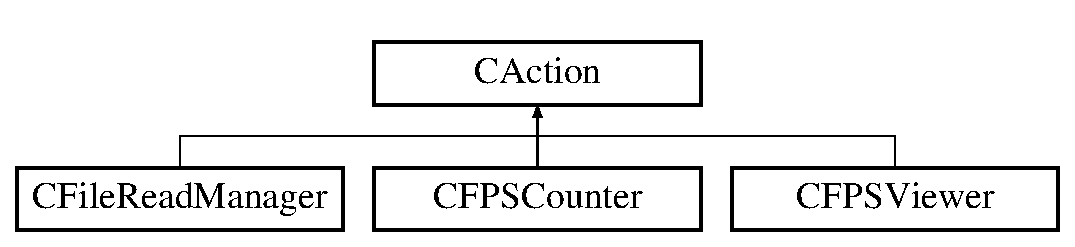
\includegraphics[height=2.000000cm]{class_c_action}
\end{center}
\end{figure}
\subsection*{公開メンバ関数}
\begin{DoxyCompactItemize}
\item 
virtual void \hyperlink{class_c_action_a3fcc5cc0fde844c5cb6e50f7eec9da3c}{Action} ()
\begin{DoxyCompactList}\small\item\em 更新処理。 \end{DoxyCompactList}\item 
void \hyperlink{class_c_action_a247d74af92f6899f99091520ece6489e}{Set\+Action\+Active} (bool \+\_\+b\+Active)
\begin{DoxyCompactList}\small\item\em アクティブフラグの設定。 \end{DoxyCompactList}\item 
bool \hyperlink{class_c_action_ac8373c1407c0078a9e755063c37d0146}{Is\+Action\+Active} () const 
\begin{DoxyCompactList}\small\item\em アクティブフラグの取得。 \end{DoxyCompactList}\item 
U32 \hyperlink{class_c_action_a601d1cdd424423b35f653cfc23120ca1}{Get\+Action\+Lv} () const 
\begin{DoxyCompactList}\small\item\em アクションレベルの取得。 \end{DoxyCompactList}\end{DoxyCompactItemize}
\subsection*{限定公開メンバ関数}
\begin{DoxyCompactItemize}
\item 
\hyperlink{class_c_action_aab25a0c59496bb5eb465d0307d7aa45a}{C\+Action} (U32 \+\_\+u\+Action\+Lv)
\begin{DoxyCompactList}\small\item\em コンストラクタ。 \end{DoxyCompactList}\item 
virtual \hyperlink{class_c_action_a45a8868d504060d8c1e8dd1f299b5854}{$\sim$\+C\+Action} ()
\begin{DoxyCompactList}\small\item\em デストラクタ。 \end{DoxyCompactList}\end{DoxyCompactItemize}
\subsection*{非公開変数類}
\begin{DoxyCompactItemize}
\item 
U32 \hyperlink{class_c_action_abb2dc369fffedd3074d99820f57c2090}{m\+\_\+u\+Action\+Lv}
\item 
bool \hyperlink{class_c_action_a55d4d949e48db21e1e1b752e8eb5c2e6}{m\+\_\+b\+Active}
\end{DoxyCompactItemize}


\subsection{詳解}
Actionを行う基底クラス。 

\subsection{構築子と解体子}
\hypertarget{class_c_action_aab25a0c59496bb5eb465d0307d7aa45a}{}\index{C\+Action@{C\+Action}!C\+Action@{C\+Action}}
\index{C\+Action@{C\+Action}!C\+Action@{C\+Action}}
\subsubsection[{C\+Action(\+U32 \+\_\+u\+Action\+Lv)}]{\setlength{\rightskip}{0pt plus 5cm}C\+Action\+::\+C\+Action (
\begin{DoxyParamCaption}
\item[{U32}]{\+\_\+u\+Action\+Lv}
\end{DoxyParamCaption}
)\hspace{0.3cm}{\ttfamily [protected]}}\label{class_c_action_aab25a0c59496bb5eb465d0307d7aa45a}


コンストラクタ。 


\begin{DoxyParams}[1]{引数}
\mbox{\tt in}  & {\em \+\_\+e\+Action\+Lv} & \+: アクションレベル。 \\
\hline
\end{DoxyParams}
\hypertarget{class_c_action_a45a8868d504060d8c1e8dd1f299b5854}{}\index{C\+Action@{C\+Action}!````~C\+Action@{$\sim$\+C\+Action}}
\index{````~C\+Action@{$\sim$\+C\+Action}!C\+Action@{C\+Action}}
\subsubsection[{$\sim$\+C\+Action()}]{\setlength{\rightskip}{0pt plus 5cm}C\+Action\+::$\sim$\+C\+Action (
\begin{DoxyParamCaption}
{}
\end{DoxyParamCaption}
)\hspace{0.3cm}{\ttfamily [protected]}, {\ttfamily [virtual]}}\label{class_c_action_a45a8868d504060d8c1e8dd1f299b5854}


デストラクタ。 



\subsection{関数詳解}
\hypertarget{class_c_action_a3fcc5cc0fde844c5cb6e50f7eec9da3c}{}\index{C\+Action@{C\+Action}!Action@{Action}}
\index{Action@{Action}!C\+Action@{C\+Action}}
\subsubsection[{Action()}]{\setlength{\rightskip}{0pt plus 5cm}virtual void C\+Action\+::\+Action (
\begin{DoxyParamCaption}
{}
\end{DoxyParamCaption}
)\hspace{0.3cm}{\ttfamily [inline]}, {\ttfamily [virtual]}}\label{class_c_action_a3fcc5cc0fde844c5cb6e50f7eec9da3c}


更新処理。 



\hyperlink{class_c_file_read_manager_a1c0c420814fed21f257b71740c56a365}{C\+File\+Read\+Manager}, \hyperlink{class_c_f_p_s_viewer_abde661517b45dbe7cd19a86ef8a0b2af}{C\+F\+P\+S\+Viewer}, \hyperlink{class_c_f_p_s_counter_acc82281b59837fb8378cbd5ef8941072}{C\+F\+P\+S\+Counter}で再実装されています。

\hypertarget{class_c_action_a601d1cdd424423b35f653cfc23120ca1}{}\index{C\+Action@{C\+Action}!Get\+Action\+Lv@{Get\+Action\+Lv}}
\index{Get\+Action\+Lv@{Get\+Action\+Lv}!C\+Action@{C\+Action}}
\subsubsection[{Get\+Action\+Lv() const }]{\setlength{\rightskip}{0pt plus 5cm}U32 C\+Action\+::\+Get\+Action\+Lv (
\begin{DoxyParamCaption}
{}
\end{DoxyParamCaption}
) const\hspace{0.3cm}{\ttfamily [inline]}}\label{class_c_action_a601d1cdd424423b35f653cfc23120ca1}


アクションレベルの取得。 

\hypertarget{class_c_action_ac8373c1407c0078a9e755063c37d0146}{}\index{C\+Action@{C\+Action}!Is\+Action\+Active@{Is\+Action\+Active}}
\index{Is\+Action\+Active@{Is\+Action\+Active}!C\+Action@{C\+Action}}
\subsubsection[{Is\+Action\+Active() const }]{\setlength{\rightskip}{0pt plus 5cm}bool C\+Action\+::\+Is\+Action\+Active (
\begin{DoxyParamCaption}
{}
\end{DoxyParamCaption}
) const\hspace{0.3cm}{\ttfamily [inline]}}\label{class_c_action_ac8373c1407c0078a9e755063c37d0146}


アクティブフラグの取得。 

\hypertarget{class_c_action_a247d74af92f6899f99091520ece6489e}{}\index{C\+Action@{C\+Action}!Set\+Action\+Active@{Set\+Action\+Active}}
\index{Set\+Action\+Active@{Set\+Action\+Active}!C\+Action@{C\+Action}}
\subsubsection[{Set\+Action\+Active(bool \+\_\+b\+Active)}]{\setlength{\rightskip}{0pt plus 5cm}void C\+Action\+::\+Set\+Action\+Active (
\begin{DoxyParamCaption}
\item[{bool}]{\+\_\+b\+Active}
\end{DoxyParamCaption}
)\hspace{0.3cm}{\ttfamily [inline]}}\label{class_c_action_a247d74af92f6899f99091520ece6489e}


アクティブフラグの設定。 



\subsection{メンバ詳解}
\hypertarget{class_c_action_a55d4d949e48db21e1e1b752e8eb5c2e6}{}\index{C\+Action@{C\+Action}!m\+\_\+b\+Active@{m\+\_\+b\+Active}}
\index{m\+\_\+b\+Active@{m\+\_\+b\+Active}!C\+Action@{C\+Action}}
\subsubsection[{m\+\_\+b\+Active}]{\setlength{\rightskip}{0pt plus 5cm}bool C\+Action\+::m\+\_\+b\+Active\hspace{0.3cm}{\ttfamily [private]}}\label{class_c_action_a55d4d949e48db21e1e1b752e8eb5c2e6}
\hypertarget{class_c_action_abb2dc369fffedd3074d99820f57c2090}{}\index{C\+Action@{C\+Action}!m\+\_\+u\+Action\+Lv@{m\+\_\+u\+Action\+Lv}}
\index{m\+\_\+u\+Action\+Lv@{m\+\_\+u\+Action\+Lv}!C\+Action@{C\+Action}}
\subsubsection[{m\+\_\+u\+Action\+Lv}]{\setlength{\rightskip}{0pt plus 5cm}U32 C\+Action\+::m\+\_\+u\+Action\+Lv\hspace{0.3cm}{\ttfamily [private]}}\label{class_c_action_abb2dc369fffedd3074d99820f57c2090}


このクラス詳解は次のファイルから抽出されました\+:\begin{DoxyCompactItemize}
\item 
D\+:/\+Project/\+Game/\+Lib/\+Object/\hyperlink{_action_8h}{Action.\+h}\item 
D\+:/\+Project/\+Game/\+Lib/\+Object/\hyperlink{_action_8cpp}{Action.\+cpp}\end{DoxyCompactItemize}

\hypertarget{class_c_action_list}{}\section{C\+Action\+List クラス}
\label{class_c_action_list}\index{C\+Action\+List@{C\+Action\+List}}


C\+Actionクラスのリスト。  




{\ttfamily \#include $<$Action\+List.\+h$>$}

C\+Action\+List の継承関係図\begin{figure}[H]
\begin{center}
\leavevmode
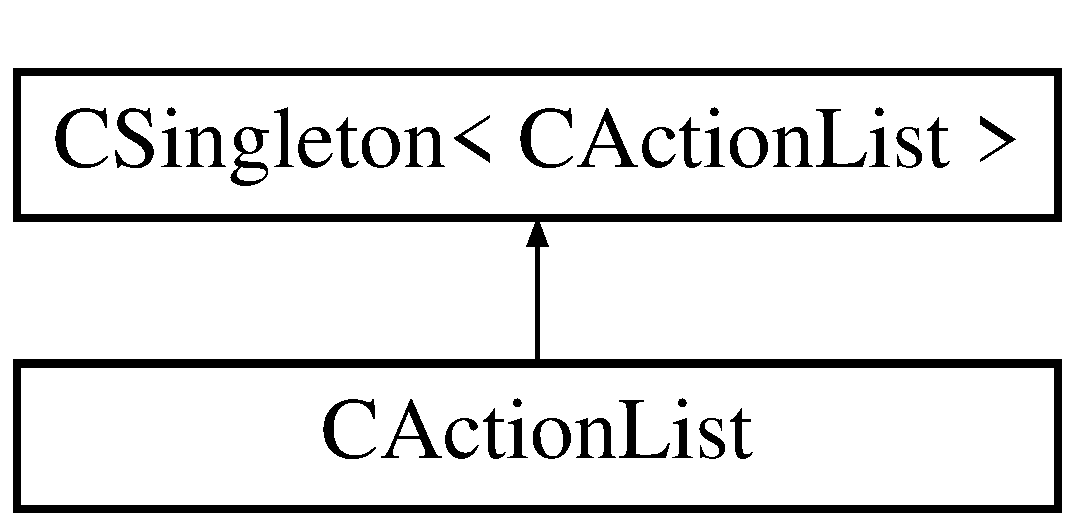
\includegraphics[height=2.000000cm]{class_c_action_list}
\end{center}
\end{figure}
\subsection*{クラス}
\begin{DoxyCompactItemize}
\item 
struct \hyperlink{struct_c_action_list_1_1_st_init_param}{St\+Init\+Param}
\begin{DoxyCompactList}\small\item\em 初期化用構造体。 \end{DoxyCompactList}\end{DoxyCompactItemize}
\subsection*{公開メンバ関数}
\begin{DoxyCompactItemize}
\item 
virtual \hyperlink{class_c_action_list_aaaa39fed12095bb0095c51d27ca19443}{$\sim$\+C\+Action\+List} ()
\begin{DoxyCompactList}\small\item\em デストラクタ。 \end{DoxyCompactList}\item 
void \hyperlink{class_c_action_list_abdfe27d4d3e92e7de8e2b91c7cf17574}{Init} (const \hyperlink{struct_c_action_list_1_1_st_init_param}{St\+Init\+Param} \&\+\_\+rst\+Param)
\begin{DoxyCompactList}\small\item\em 初期化。 \end{DoxyCompactList}\item 
void \hyperlink{class_c_action_list_aa1341ee2595b0c1ae226123dccef0477}{Register} (\hyperlink{class_c_action}{C\+Action} $\ast$\+\_\+p\+Object)
\begin{DoxyCompactList}\small\item\em 登録処理。 \end{DoxyCompactList}\item 
void \hyperlink{class_c_action_list_a916677de8c5f6c39846f46800ef0f0e7}{Un\+Register} (\hyperlink{class_c_action}{C\+Action} $\ast$\+\_\+p\+Object)
\begin{DoxyCompactList}\small\item\em 解除処理。 \end{DoxyCompactList}\item 
void \hyperlink{class_c_action_list_aa3d82dc70353a5fc2dd10fc6a2800f85}{All\+Action} ()
\begin{DoxyCompactList}\small\item\em 登録された全てのオブジェクトのアクションを実行。 \end{DoxyCompactList}\end{DoxyCompactItemize}
\subsection*{非公開メンバ関数}
\begin{DoxyCompactItemize}
\item 
\hyperlink{class_c_action_list_ae814ffecb31176127c16fbf8b8619853}{C\+Action\+List} ()
\begin{DoxyCompactList}\small\item\em コンストラクタ。 \end{DoxyCompactList}\end{DoxyCompactItemize}
\subsection*{非公開変数類}
\begin{DoxyCompactItemize}
\item 
friend \hyperlink{class_c_action_list_ab1bfb7078790f77dbf03457598b13e90}{C\+Singleton$<$ C\+Action\+List $>$}
\item 
\hyperlink{struct_c_action_list_1_1_st_init_param}{St\+Init\+Param} \hyperlink{class_c_action_list_a32027728142c6e1af28240a59ed009bb}{m\+\_\+st\+Param}
\item 
\hyperlink{class_c_object_list}{C\+Object\+List}$<$ \hyperlink{class_c_action}{C\+Action} $>$ $\ast$ \hyperlink{class_c_action_list_ac374ad0c0bc4b0d86a4a33064f16b1dc}{m\+\_\+pc\+Action\+List}
\end{DoxyCompactItemize}
\subsection*{その他の継承メンバ}


\subsection{詳解}
C\+Actionクラスのリスト。 

\subsection{構築子と解体子}
\hypertarget{class_c_action_list_ae814ffecb31176127c16fbf8b8619853}{}\index{C\+Action\+List@{C\+Action\+List}!C\+Action\+List@{C\+Action\+List}}
\index{C\+Action\+List@{C\+Action\+List}!C\+Action\+List@{C\+Action\+List}}
\subsubsection[{C\+Action\+List()}]{\setlength{\rightskip}{0pt plus 5cm}C\+Action\+List\+::\+C\+Action\+List (
\begin{DoxyParamCaption}
{}
\end{DoxyParamCaption}
)\hspace{0.3cm}{\ttfamily [private]}}\label{class_c_action_list_ae814ffecb31176127c16fbf8b8619853}


コンストラクタ。 

\hypertarget{class_c_action_list_aaaa39fed12095bb0095c51d27ca19443}{}\index{C\+Action\+List@{C\+Action\+List}!````~C\+Action\+List@{$\sim$\+C\+Action\+List}}
\index{````~C\+Action\+List@{$\sim$\+C\+Action\+List}!C\+Action\+List@{C\+Action\+List}}
\subsubsection[{$\sim$\+C\+Action\+List()}]{\setlength{\rightskip}{0pt plus 5cm}C\+Action\+List\+::$\sim$\+C\+Action\+List (
\begin{DoxyParamCaption}
{}
\end{DoxyParamCaption}
)\hspace{0.3cm}{\ttfamily [virtual]}}\label{class_c_action_list_aaaa39fed12095bb0095c51d27ca19443}


デストラクタ。 



\subsection{関数詳解}
\hypertarget{class_c_action_list_aa3d82dc70353a5fc2dd10fc6a2800f85}{}\index{C\+Action\+List@{C\+Action\+List}!All\+Action@{All\+Action}}
\index{All\+Action@{All\+Action}!C\+Action\+List@{C\+Action\+List}}
\subsubsection[{All\+Action()}]{\setlength{\rightskip}{0pt plus 5cm}void C\+Action\+List\+::\+All\+Action (
\begin{DoxyParamCaption}
{}
\end{DoxyParamCaption}
)}\label{class_c_action_list_aa3d82dc70353a5fc2dd10fc6a2800f85}


登録された全てのオブジェクトのアクションを実行。 

\hypertarget{class_c_action_list_abdfe27d4d3e92e7de8e2b91c7cf17574}{}\index{C\+Action\+List@{C\+Action\+List}!Init@{Init}}
\index{Init@{Init}!C\+Action\+List@{C\+Action\+List}}
\subsubsection[{Init(const St\+Init\+Param \&\+\_\+rst\+Param)}]{\setlength{\rightskip}{0pt plus 5cm}void C\+Action\+List\+::\+Init (
\begin{DoxyParamCaption}
\item[{const {\bf St\+Init\+Param} \&}]{\+\_\+rst\+Param}
\end{DoxyParamCaption}
)}\label{class_c_action_list_abdfe27d4d3e92e7de8e2b91c7cf17574}


初期化。 


\begin{DoxyParams}[1]{引数}
\mbox{\tt in}  & {\em \+\_\+rst\+Param} & \+: 初期化用パラメータ。 \\
\hline
\end{DoxyParams}
\hypertarget{class_c_action_list_aa1341ee2595b0c1ae226123dccef0477}{}\index{C\+Action\+List@{C\+Action\+List}!Register@{Register}}
\index{Register@{Register}!C\+Action\+List@{C\+Action\+List}}
\subsubsection[{Register(\+C\+Action $\ast$\+\_\+p\+Object)}]{\setlength{\rightskip}{0pt plus 5cm}void C\+Action\+List\+::\+Register (
\begin{DoxyParamCaption}
\item[{{\bf C\+Action} $\ast$}]{\+\_\+p\+Object}
\end{DoxyParamCaption}
)}\label{class_c_action_list_aa1341ee2595b0c1ae226123dccef0477}


登録処理。 


\begin{DoxyParams}[1]{引数}
\mbox{\tt in}  & {\em \+\_\+p\+Objcet} & \+: 登録するオブジェクト。 \\
\hline
\end{DoxyParams}
\hypertarget{class_c_action_list_a916677de8c5f6c39846f46800ef0f0e7}{}\index{C\+Action\+List@{C\+Action\+List}!Un\+Register@{Un\+Register}}
\index{Un\+Register@{Un\+Register}!C\+Action\+List@{C\+Action\+List}}
\subsubsection[{Un\+Register(\+C\+Action $\ast$\+\_\+p\+Object)}]{\setlength{\rightskip}{0pt plus 5cm}void C\+Action\+List\+::\+Un\+Register (
\begin{DoxyParamCaption}
\item[{{\bf C\+Action} $\ast$}]{\+\_\+p\+Object}
\end{DoxyParamCaption}
)}\label{class_c_action_list_a916677de8c5f6c39846f46800ef0f0e7}


解除処理。 


\begin{DoxyParams}[1]{引数}
\mbox{\tt in}  & {\em \+\_\+p\+Objcet} & \+: 解除するオブジェクト。 \\
\hline
\end{DoxyParams}


\subsection{メンバ詳解}
\hypertarget{class_c_action_list_ab1bfb7078790f77dbf03457598b13e90}{}\index{C\+Action\+List@{C\+Action\+List}!C\+Singleton$<$ C\+Action\+List $>$@{C\+Singleton$<$ C\+Action\+List $>$}}
\index{C\+Singleton$<$ C\+Action\+List $>$@{C\+Singleton$<$ C\+Action\+List $>$}!C\+Action\+List@{C\+Action\+List}}
\subsubsection[{C\+Singleton$<$ C\+Action\+List $>$}]{\setlength{\rightskip}{0pt plus 5cm}friend {\bf C\+Action\+List\+::\+C\+Singleton}$<$ {\bf C\+Action\+List} $>$\hspace{0.3cm}{\ttfamily [private]}}\label{class_c_action_list_ab1bfb7078790f77dbf03457598b13e90}
\hypertarget{class_c_action_list_ac374ad0c0bc4b0d86a4a33064f16b1dc}{}\index{C\+Action\+List@{C\+Action\+List}!m\+\_\+pc\+Action\+List@{m\+\_\+pc\+Action\+List}}
\index{m\+\_\+pc\+Action\+List@{m\+\_\+pc\+Action\+List}!C\+Action\+List@{C\+Action\+List}}
\subsubsection[{m\+\_\+pc\+Action\+List}]{\setlength{\rightskip}{0pt plus 5cm}{\bf C\+Object\+List}$<${\bf C\+Action}$>$$\ast$ C\+Action\+List\+::m\+\_\+pc\+Action\+List\hspace{0.3cm}{\ttfamily [private]}}\label{class_c_action_list_ac374ad0c0bc4b0d86a4a33064f16b1dc}
\hypertarget{class_c_action_list_a32027728142c6e1af28240a59ed009bb}{}\index{C\+Action\+List@{C\+Action\+List}!m\+\_\+st\+Param@{m\+\_\+st\+Param}}
\index{m\+\_\+st\+Param@{m\+\_\+st\+Param}!C\+Action\+List@{C\+Action\+List}}
\subsubsection[{m\+\_\+st\+Param}]{\setlength{\rightskip}{0pt plus 5cm}{\bf St\+Init\+Param} C\+Action\+List\+::m\+\_\+st\+Param\hspace{0.3cm}{\ttfamily [private]}}\label{class_c_action_list_a32027728142c6e1af28240a59ed009bb}


このクラス詳解は次のファイルから抽出されました\+:\begin{DoxyCompactItemize}
\item 
D\+:/\+Project/\+Game/\+Lib/\+Object/\hyperlink{_action_list_8h}{Action\+List.\+h}\item 
D\+:/\+Project/\+Game/\+Lib/\+Object/\hyperlink{_action_list_8cpp}{Action\+List.\+cpp}\end{DoxyCompactItemize}

\hypertarget{class_c_action_lv}{}\section{C\+Action\+Lv クラス}
\label{class_c_action_lv}\index{C\+Action\+Lv@{C\+Action\+Lv}}


{\ttfamily \#include $<$Action\+Lv.\+h$>$}

\subsection*{公開型}
\begin{DoxyCompactItemize}
\item 
enum \hyperlink{class_c_action_lv_a1749377d2117848013fb5373d9d11750}{En\+Action\+Lv} \+: U32 \{ \hyperlink{class_c_action_lv_a1749377d2117848013fb5373d9d11750aa45da96d0bf6575970f2d27af22be28a}{En\+Action\+Lv\+::\+System} = 0, 
\hyperlink{class_c_action_lv_a1749377d2117848013fb5373d9d11750a960b44c579bc2f6818d2daaf9e4c16f0}{En\+Action\+Lv\+::\+Normal}, 
\hyperlink{class_c_action_lv_a1749377d2117848013fb5373d9d11750a6a061313d22e51e0f25b7cd4dc065233}{En\+Action\+Lv\+::\+Max}
 \}
\end{DoxyCompactItemize}
\subsection*{静的公開メンバ関数}
\begin{DoxyCompactItemize}
\item 
static U32 \hyperlink{class_c_action_lv_a0d923aa2f7e279e4210c739382fe09eb}{System} ()
\item 
static U32 \hyperlink{class_c_action_lv_a1c31162c00a28a339327154a594736bb}{Normaml} ()
\item 
static U32 \hyperlink{class_c_action_lv_ac4d8fa4b57fd7c12533b64ffc8891115}{Max} ()
\end{DoxyCompactItemize}


\subsection{列挙型メンバ詳解}
\hypertarget{class_c_action_lv_a1749377d2117848013fb5373d9d11750}{}\index{C\+Action\+Lv@{C\+Action\+Lv}!En\+Action\+Lv@{En\+Action\+Lv}}
\index{En\+Action\+Lv@{En\+Action\+Lv}!C\+Action\+Lv@{C\+Action\+Lv}}
\subsubsection[{En\+Action\+Lv}]{\setlength{\rightskip}{0pt plus 5cm}enum {\bf C\+Action\+Lv\+::\+En\+Action\+Lv} \+: U32\hspace{0.3cm}{\ttfamily [strong]}}\label{class_c_action_lv_a1749377d2117848013fb5373d9d11750}
\begin{Desc}
\item[列挙値]\par
\begin{description}
\index{System@{System}!C\+Action\+Lv@{C\+Action\+Lv}}\index{C\+Action\+Lv@{C\+Action\+Lv}!System@{System}}\item[{\em 
\hypertarget{class_c_action_lv_a1749377d2117848013fb5373d9d11750aa45da96d0bf6575970f2d27af22be28a}{}System\label{class_c_action_lv_a1749377d2117848013fb5373d9d11750aa45da96d0bf6575970f2d27af22be28a}
}]\index{Normal@{Normal}!C\+Action\+Lv@{C\+Action\+Lv}}\index{C\+Action\+Lv@{C\+Action\+Lv}!Normal@{Normal}}\item[{\em 
\hypertarget{class_c_action_lv_a1749377d2117848013fb5373d9d11750a960b44c579bc2f6818d2daaf9e4c16f0}{}Normal\label{class_c_action_lv_a1749377d2117848013fb5373d9d11750a960b44c579bc2f6818d2daaf9e4c16f0}
}]\index{Max@{Max}!C\+Action\+Lv@{C\+Action\+Lv}}\index{C\+Action\+Lv@{C\+Action\+Lv}!Max@{Max}}\item[{\em 
\hypertarget{class_c_action_lv_a1749377d2117848013fb5373d9d11750a6a061313d22e51e0f25b7cd4dc065233}{}Max\label{class_c_action_lv_a1749377d2117848013fb5373d9d11750a6a061313d22e51e0f25b7cd4dc065233}
}]\end{description}
\end{Desc}


\subsection{関数詳解}
\hypertarget{class_c_action_lv_ac4d8fa4b57fd7c12533b64ffc8891115}{}\index{C\+Action\+Lv@{C\+Action\+Lv}!Max@{Max}}
\index{Max@{Max}!C\+Action\+Lv@{C\+Action\+Lv}}
\subsubsection[{Max()}]{\setlength{\rightskip}{0pt plus 5cm}static U32 C\+Action\+Lv\+::\+Max (
\begin{DoxyParamCaption}
{}
\end{DoxyParamCaption}
)\hspace{0.3cm}{\ttfamily [inline]}, {\ttfamily [static]}}\label{class_c_action_lv_ac4d8fa4b57fd7c12533b64ffc8891115}
\hypertarget{class_c_action_lv_a1c31162c00a28a339327154a594736bb}{}\index{C\+Action\+Lv@{C\+Action\+Lv}!Normaml@{Normaml}}
\index{Normaml@{Normaml}!C\+Action\+Lv@{C\+Action\+Lv}}
\subsubsection[{Normaml()}]{\setlength{\rightskip}{0pt plus 5cm}static U32 C\+Action\+Lv\+::\+Normaml (
\begin{DoxyParamCaption}
{}
\end{DoxyParamCaption}
)\hspace{0.3cm}{\ttfamily [inline]}, {\ttfamily [static]}}\label{class_c_action_lv_a1c31162c00a28a339327154a594736bb}
\hypertarget{class_c_action_lv_a0d923aa2f7e279e4210c739382fe09eb}{}\index{C\+Action\+Lv@{C\+Action\+Lv}!System@{System}}
\index{System@{System}!C\+Action\+Lv@{C\+Action\+Lv}}
\subsubsection[{System()}]{\setlength{\rightskip}{0pt plus 5cm}static U32 C\+Action\+Lv\+::\+System (
\begin{DoxyParamCaption}
{}
\end{DoxyParamCaption}
)\hspace{0.3cm}{\ttfamily [inline]}, {\ttfamily [static]}}\label{class_c_action_lv_a0d923aa2f7e279e4210c739382fe09eb}


このクラス詳解は次のファイルから抽出されました\+:\begin{DoxyCompactItemize}
\item 
D\+:/\+Project/\+Game/\hyperlink{_action_lv_8h}{Action\+Lv.\+h}\end{DoxyCompactItemize}

\hypertarget{class_c_allocator}{}\section{C\+Allocator$<$ T $>$ クラステンプレート}
\label{class_c_allocator}\index{C\+Allocator$<$ T $>$@{C\+Allocator$<$ T $>$}}


{\ttfamily \#include $<$Allocator.\+h$>$}

C\+Allocator$<$ T $>$ の継承関係図\begin{figure}[H]
\begin{center}
\leavevmode
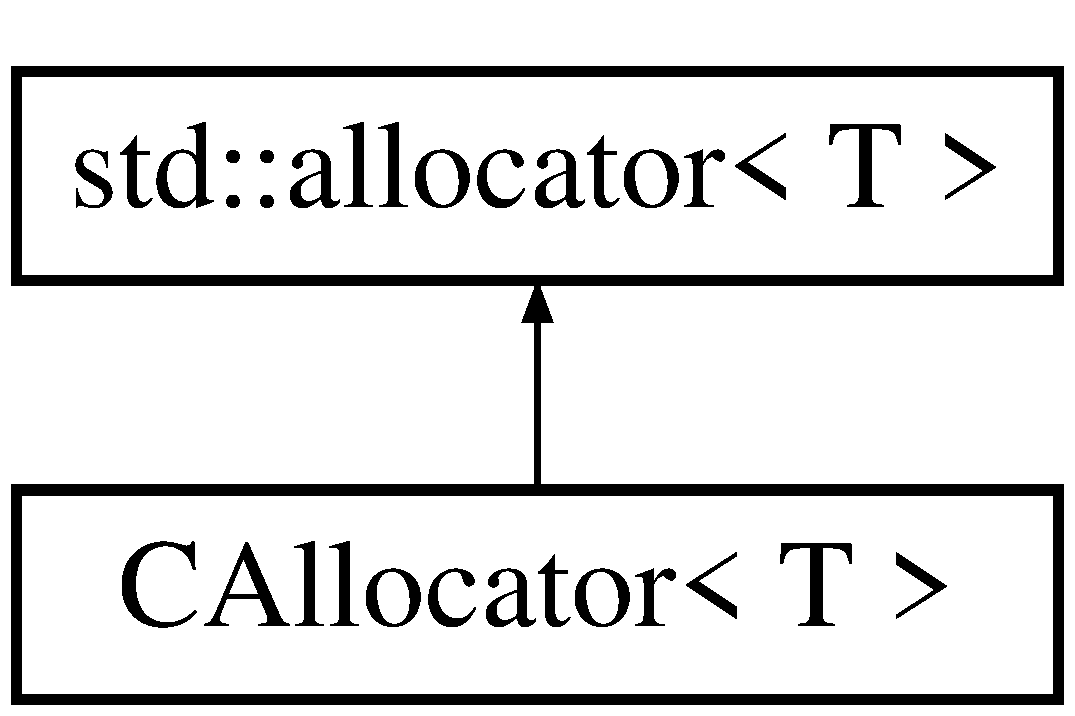
\includegraphics[height=2.000000cm]{class_c_allocator}
\end{center}
\end{figure}
\subsection*{クラス}
\begin{DoxyCompactItemize}
\item 
struct \hyperlink{struct_c_allocator_1_1rebind}{rebind}
\end{DoxyCompactItemize}
\subsection*{公開メンバ関数}
\begin{DoxyCompactItemize}
\item 
\hyperlink{class_c_allocator_ac47a279ea8fcbd55f7c8df3044bf93ff}{C\+Allocator} ()
\begin{DoxyCompactList}\small\item\em コンストラクタ。 \end{DoxyCompactList}\item 
{\footnotesize template$<$class U $>$ }\\\hyperlink{class_c_allocator_a7ee93416bbf19a9a20ad9f971208a2d3}{C\+Allocator} (const \hyperlink{class_c_allocator}{C\+Allocator}$<$ U $>$ \&\+\_\+r\+Allocator)
\item 
\hyperlink{class_c_allocator_ab62db0893a3119e3f99d29f3adfe9565}{$\sim$\+C\+Allocator} ()
\begin{DoxyCompactList}\small\item\em デストラクタ。 \end{DoxyCompactList}\item 
pointer \hyperlink{class_c_allocator_a2d88f40d4a8e61088ad90aa779c2b9dc}{allocate} (size\+\_\+type \+\_\+u\+Num, const\+\_\+pointer \+\_\+hint=0)
\begin{DoxyCompactList}\small\item\em メモリの確保。 \end{DoxyCompactList}\item 
void \hyperlink{class_c_allocator_ac85aa74964df1ac149878fb68ed5017a}{deallocate} (pointer \+\_\+p, size\+\_\+type \+\_\+u\+Num)
\begin{DoxyCompactList}\small\item\em メモリの解放。 \end{DoxyCompactList}\end{DoxyCompactItemize}


\subsection{構築子と解体子}
\hypertarget{class_c_allocator_ac47a279ea8fcbd55f7c8df3044bf93ff}{}\index{C\+Allocator@{C\+Allocator}!C\+Allocator@{C\+Allocator}}
\index{C\+Allocator@{C\+Allocator}!C\+Allocator@{C\+Allocator}}
\subsubsection[{C\+Allocator()}]{\setlength{\rightskip}{0pt plus 5cm}template$<$class T$>$ {\bf C\+Allocator}$<$ T $>$\+::{\bf C\+Allocator} (
\begin{DoxyParamCaption}
{}
\end{DoxyParamCaption}
)\hspace{0.3cm}{\ttfamily [inline]}}\label{class_c_allocator_ac47a279ea8fcbd55f7c8df3044bf93ff}


コンストラクタ。 

\hypertarget{class_c_allocator_a7ee93416bbf19a9a20ad9f971208a2d3}{}\index{C\+Allocator@{C\+Allocator}!C\+Allocator@{C\+Allocator}}
\index{C\+Allocator@{C\+Allocator}!C\+Allocator@{C\+Allocator}}
\subsubsection[{C\+Allocator(const C\+Allocator$<$ U $>$ \&\+\_\+r\+Allocator)}]{\setlength{\rightskip}{0pt plus 5cm}template$<$class T$>$ template$<$class U $>$ {\bf C\+Allocator}$<$ T $>$\+::{\bf C\+Allocator} (
\begin{DoxyParamCaption}
\item[{const {\bf C\+Allocator}$<$ U $>$ \&}]{\+\_\+r\+Allocator}
\end{DoxyParamCaption}
)\hspace{0.3cm}{\ttfamily [inline]}}\label{class_c_allocator_a7ee93416bbf19a9a20ad9f971208a2d3}
\hypertarget{class_c_allocator_ab62db0893a3119e3f99d29f3adfe9565}{}\index{C\+Allocator@{C\+Allocator}!````~C\+Allocator@{$\sim$\+C\+Allocator}}
\index{````~C\+Allocator@{$\sim$\+C\+Allocator}!C\+Allocator@{C\+Allocator}}
\subsubsection[{$\sim$\+C\+Allocator()}]{\setlength{\rightskip}{0pt plus 5cm}template$<$class T$>$ {\bf C\+Allocator}$<$ T $>$\+::$\sim${\bf C\+Allocator} (
\begin{DoxyParamCaption}
{}
\end{DoxyParamCaption}
)\hspace{0.3cm}{\ttfamily [inline]}}\label{class_c_allocator_ab62db0893a3119e3f99d29f3adfe9565}


デストラクタ。 



\subsection{関数詳解}
\hypertarget{class_c_allocator_a2d88f40d4a8e61088ad90aa779c2b9dc}{}\index{C\+Allocator@{C\+Allocator}!allocate@{allocate}}
\index{allocate@{allocate}!C\+Allocator@{C\+Allocator}}
\subsubsection[{allocate(size\+\_\+type \+\_\+u\+Num, const\+\_\+pointer \+\_\+hint=0)}]{\setlength{\rightskip}{0pt plus 5cm}template$<$class T$>$ pointer {\bf C\+Allocator}$<$ T $>$\+::allocate (
\begin{DoxyParamCaption}
\item[{size\+\_\+type}]{\+\_\+u\+Num, }
\item[{const\+\_\+pointer}]{\+\_\+hint = {\ttfamily 0}}
\end{DoxyParamCaption}
)\hspace{0.3cm}{\ttfamily [inline]}}\label{class_c_allocator_a2d88f40d4a8e61088ad90aa779c2b9dc}


メモリの確保。 

\hypertarget{class_c_allocator_ac85aa74964df1ac149878fb68ed5017a}{}\index{C\+Allocator@{C\+Allocator}!deallocate@{deallocate}}
\index{deallocate@{deallocate}!C\+Allocator@{C\+Allocator}}
\subsubsection[{deallocate(pointer \+\_\+p, size\+\_\+type \+\_\+u\+Num)}]{\setlength{\rightskip}{0pt plus 5cm}template$<$class T$>$ void {\bf C\+Allocator}$<$ T $>$\+::deallocate (
\begin{DoxyParamCaption}
\item[{pointer}]{\+\_\+p, }
\item[{size\+\_\+type}]{\+\_\+u\+Num}
\end{DoxyParamCaption}
)\hspace{0.3cm}{\ttfamily [inline]}}\label{class_c_allocator_ac85aa74964df1ac149878fb68ed5017a}


メモリの解放。 



このクラス詳解は次のファイルから抽出されました\+:\begin{DoxyCompactItemize}
\item 
D\+:/\+Project/\+Game/\+Lib/\+Memory/\+Allocator/\hyperlink{_allocator_8h}{Allocator.\+h}\end{DoxyCompactItemize}

\hypertarget{class_c_constant_buffer_for_frame}{}\section{C\+Constant\+Buffer\+For\+Frame クラス}
\label{class_c_constant_buffer_for_frame}\index{C\+Constant\+Buffer\+For\+Frame@{C\+Constant\+Buffer\+For\+Frame}}


{\ttfamily \#include $<$Constant\+Buffer\+For\+Frame.\+h$>$}

C\+Constant\+Buffer\+For\+Frame の継承関係図\begin{figure}[H]
\begin{center}
\leavevmode
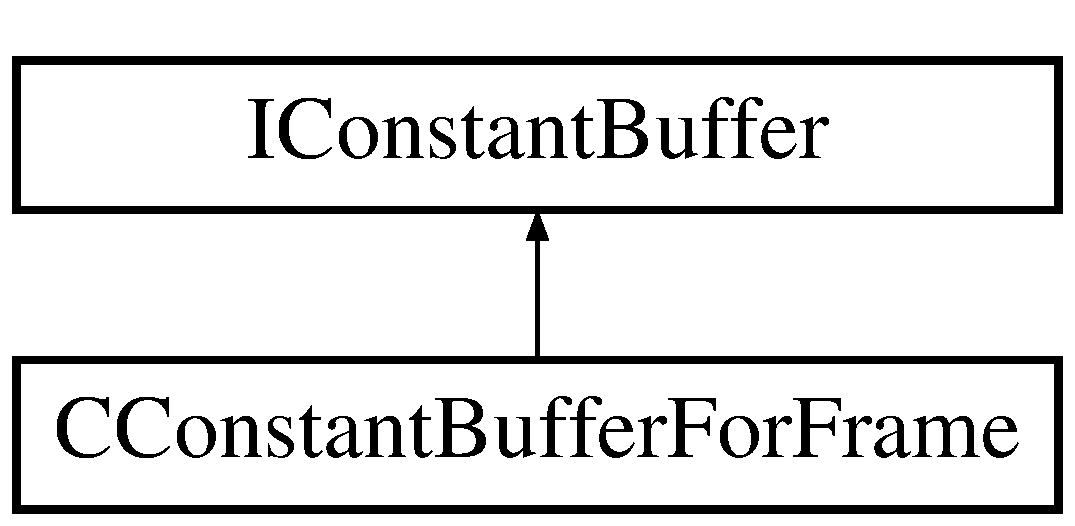
\includegraphics[height=2.000000cm]{class_c_constant_buffer_for_frame}
\end{center}
\end{figure}
\subsection*{クラス}
\begin{DoxyCompactItemize}
\item 
struct \hyperlink{struct_c_constant_buffer_for_frame_1_1_st_constant_buffer}{St\+Constant\+Buffer}
\begin{DoxyCompactList}\small\item\em コンスタントバッファー構造体。 \end{DoxyCompactList}\end{DoxyCompactItemize}
\subsection*{公開メンバ関数}
\begin{DoxyCompactItemize}
\item 
\hyperlink{class_c_constant_buffer_for_frame_ae154fb95df517a7cf0bc1bb8ca4c8a92}{C\+Constant\+Buffer\+For\+Frame} ()
\begin{DoxyCompactList}\small\item\em コンストラクタ。 \end{DoxyCompactList}\item 
virtual \hyperlink{class_c_constant_buffer_for_frame_aa82763ae45d9d8f4e1f515a1a88809fe}{$\sim$\+C\+Constant\+Buffer\+For\+Frame} ()
\begin{DoxyCompactList}\small\item\em デストラクタ。 \end{DoxyCompactList}\item 
virtual const void $\ast$ \hyperlink{class_c_constant_buffer_for_frame_a1dd7a17aa4584865227d2e4188693da9}{Get\+Data} () const  override
\begin{DoxyCompactList}\small\item\em データを取得。 \end{DoxyCompactList}\item 
virtual U\+Size \hyperlink{class_c_constant_buffer_for_frame_afbfb7c7b533d75dc65e01a3f873d6e71}{Get\+Size} () const  override
\begin{DoxyCompactList}\small\item\em データサイズを取得。 \end{DoxyCompactList}\end{DoxyCompactItemize}
\subsection*{非公開変数類}
\begin{DoxyCompactItemize}
\item 
\hyperlink{struct_c_constant_buffer_for_frame_1_1_st_constant_buffer}{St\+Constant\+Buffer} \hyperlink{class_c_constant_buffer_for_frame_aa5f6bf35a4dfbefdde7ac0d80c9b8214}{m\+\_\+st\+Buffer}
\end{DoxyCompactItemize}


\subsection{構築子と解体子}
\hypertarget{class_c_constant_buffer_for_frame_ae154fb95df517a7cf0bc1bb8ca4c8a92}{}\index{C\+Constant\+Buffer\+For\+Frame@{C\+Constant\+Buffer\+For\+Frame}!C\+Constant\+Buffer\+For\+Frame@{C\+Constant\+Buffer\+For\+Frame}}
\index{C\+Constant\+Buffer\+For\+Frame@{C\+Constant\+Buffer\+For\+Frame}!C\+Constant\+Buffer\+For\+Frame@{C\+Constant\+Buffer\+For\+Frame}}
\subsubsection[{C\+Constant\+Buffer\+For\+Frame()}]{\setlength{\rightskip}{0pt plus 5cm}C\+Constant\+Buffer\+For\+Frame\+::\+C\+Constant\+Buffer\+For\+Frame (
\begin{DoxyParamCaption}
{}
\end{DoxyParamCaption}
)}\label{class_c_constant_buffer_for_frame_ae154fb95df517a7cf0bc1bb8ca4c8a92}


コンストラクタ。 

\hypertarget{class_c_constant_buffer_for_frame_aa82763ae45d9d8f4e1f515a1a88809fe}{}\index{C\+Constant\+Buffer\+For\+Frame@{C\+Constant\+Buffer\+For\+Frame}!````~C\+Constant\+Buffer\+For\+Frame@{$\sim$\+C\+Constant\+Buffer\+For\+Frame}}
\index{````~C\+Constant\+Buffer\+For\+Frame@{$\sim$\+C\+Constant\+Buffer\+For\+Frame}!C\+Constant\+Buffer\+For\+Frame@{C\+Constant\+Buffer\+For\+Frame}}
\subsubsection[{$\sim$\+C\+Constant\+Buffer\+For\+Frame()}]{\setlength{\rightskip}{0pt plus 5cm}virtual C\+Constant\+Buffer\+For\+Frame\+::$\sim$\+C\+Constant\+Buffer\+For\+Frame (
\begin{DoxyParamCaption}
{}
\end{DoxyParamCaption}
)\hspace{0.3cm}{\ttfamily [inline]}, {\ttfamily [virtual]}}\label{class_c_constant_buffer_for_frame_aa82763ae45d9d8f4e1f515a1a88809fe}


デストラクタ。 



\subsection{関数詳解}
\hypertarget{class_c_constant_buffer_for_frame_a1dd7a17aa4584865227d2e4188693da9}{}\index{C\+Constant\+Buffer\+For\+Frame@{C\+Constant\+Buffer\+For\+Frame}!Get\+Data@{Get\+Data}}
\index{Get\+Data@{Get\+Data}!C\+Constant\+Buffer\+For\+Frame@{C\+Constant\+Buffer\+For\+Frame}}
\subsubsection[{Get\+Data() const  override}]{\setlength{\rightskip}{0pt plus 5cm}virtual const void$\ast$ C\+Constant\+Buffer\+For\+Frame\+::\+Get\+Data (
\begin{DoxyParamCaption}
{}
\end{DoxyParamCaption}
) const\hspace{0.3cm}{\ttfamily [inline]}, {\ttfamily [override]}, {\ttfamily [virtual]}}\label{class_c_constant_buffer_for_frame_a1dd7a17aa4584865227d2e4188693da9}


データを取得。 



\hyperlink{class_i_constant_buffer_a51d7e72f262e74f2018b480102dc795e}{I\+Constant\+Buffer}を実装しています。

\hypertarget{class_c_constant_buffer_for_frame_afbfb7c7b533d75dc65e01a3f873d6e71}{}\index{C\+Constant\+Buffer\+For\+Frame@{C\+Constant\+Buffer\+For\+Frame}!Get\+Size@{Get\+Size}}
\index{Get\+Size@{Get\+Size}!C\+Constant\+Buffer\+For\+Frame@{C\+Constant\+Buffer\+For\+Frame}}
\subsubsection[{Get\+Size() const  override}]{\setlength{\rightskip}{0pt plus 5cm}virtual U\+Size C\+Constant\+Buffer\+For\+Frame\+::\+Get\+Size (
\begin{DoxyParamCaption}
{}
\end{DoxyParamCaption}
) const\hspace{0.3cm}{\ttfamily [inline]}, {\ttfamily [override]}, {\ttfamily [virtual]}}\label{class_c_constant_buffer_for_frame_afbfb7c7b533d75dc65e01a3f873d6e71}


データサイズを取得。 



\hyperlink{class_i_constant_buffer_a527035ebacd73ffe5c5856f75220ac68}{I\+Constant\+Buffer}を実装しています。



\subsection{メンバ詳解}
\hypertarget{class_c_constant_buffer_for_frame_aa5f6bf35a4dfbefdde7ac0d80c9b8214}{}\index{C\+Constant\+Buffer\+For\+Frame@{C\+Constant\+Buffer\+For\+Frame}!m\+\_\+st\+Buffer@{m\+\_\+st\+Buffer}}
\index{m\+\_\+st\+Buffer@{m\+\_\+st\+Buffer}!C\+Constant\+Buffer\+For\+Frame@{C\+Constant\+Buffer\+For\+Frame}}
\subsubsection[{m\+\_\+st\+Buffer}]{\setlength{\rightskip}{0pt plus 5cm}{\bf St\+Constant\+Buffer} C\+Constant\+Buffer\+For\+Frame\+::m\+\_\+st\+Buffer\hspace{0.3cm}{\ttfamily [private]}}\label{class_c_constant_buffer_for_frame_aa5f6bf35a4dfbefdde7ac0d80c9b8214}


このクラス詳解は次のファイルから抽出されました\+:\begin{DoxyCompactItemize}
\item 
D\+:/\+Project/\+Game/\+Lib/\+Render/\hyperlink{_constant_buffer_for_frame_8h}{Constant\+Buffer\+For\+Frame.\+h}\item 
D\+:/\+Project/\+Game/\+Lib/\+Render/\hyperlink{_constant_buffer_for_frame_8cpp}{Constant\+Buffer\+For\+Frame.\+cpp}\end{DoxyCompactItemize}

\hypertarget{class_c_constant_buffer_for_level}{}\section{C\+Constant\+Buffer\+For\+Level クラス}
\label{class_c_constant_buffer_for_level}\index{C\+Constant\+Buffer\+For\+Level@{C\+Constant\+Buffer\+For\+Level}}


{\ttfamily \#include $<$Constant\+Buffer\+For\+Level.\+h$>$}

C\+Constant\+Buffer\+For\+Level の継承関係図\begin{figure}[H]
\begin{center}
\leavevmode
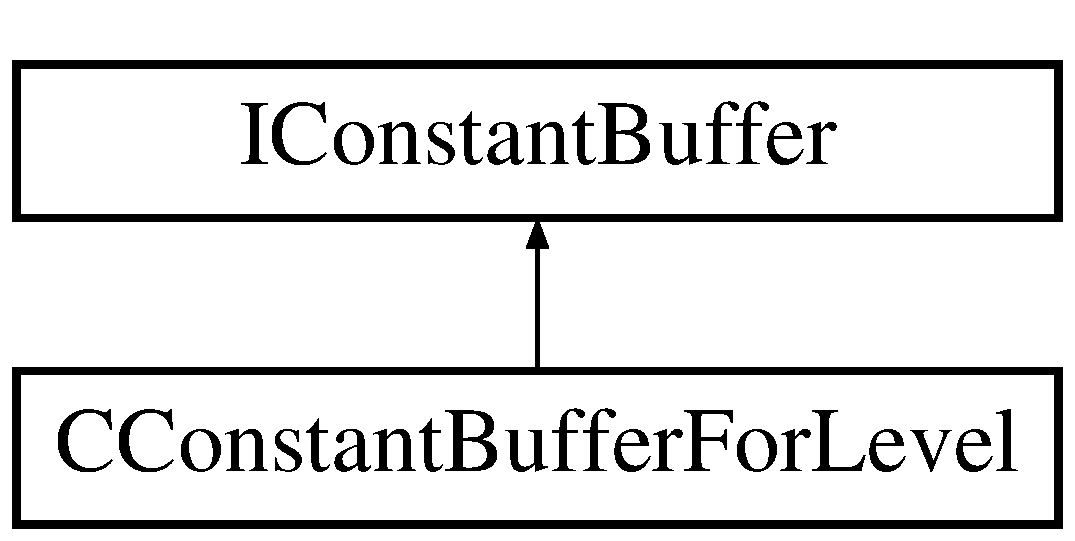
\includegraphics[height=2.000000cm]{class_c_constant_buffer_for_level}
\end{center}
\end{figure}
\subsection*{クラス}
\begin{DoxyCompactItemize}
\item 
struct \hyperlink{struct_c_constant_buffer_for_level_1_1_st_constant_buffer}{St\+Constant\+Buffer}
\begin{DoxyCompactList}\small\item\em コンスタントバッファー構造体。 \end{DoxyCompactList}\end{DoxyCompactItemize}
\subsection*{公開メンバ関数}
\begin{DoxyCompactItemize}
\item 
\hyperlink{class_c_constant_buffer_for_level_a6dfcab6b58a853ba7225240a017753f8}{C\+Constant\+Buffer\+For\+Level} ()
\begin{DoxyCompactList}\small\item\em コンストラクタ。 \end{DoxyCompactList}\item 
virtual \hyperlink{class_c_constant_buffer_for_level_aef0faa964f193e24f9ce6b39dc17da89}{$\sim$\+C\+Constant\+Buffer\+For\+Level} ()
\begin{DoxyCompactList}\small\item\em デストラクタ。 \end{DoxyCompactList}\item 
virtual const void $\ast$ \hyperlink{class_c_constant_buffer_for_level_a2de25b6e96d4ed77ab5e598389b3bd08}{Get\+Data} () const  override
\begin{DoxyCompactList}\small\item\em データを取得。 \end{DoxyCompactList}\item 
virtual U\+Size \hyperlink{class_c_constant_buffer_for_level_a5d653c0978f370dcef86eece263871dd}{Get\+Size} () const  override
\begin{DoxyCompactList}\small\item\em データサイズを取得。 \end{DoxyCompactList}\end{DoxyCompactItemize}
\subsection*{非公開変数類}
\begin{DoxyCompactItemize}
\item 
\hyperlink{struct_c_constant_buffer_for_level_1_1_st_constant_buffer}{St\+Constant\+Buffer} \hyperlink{class_c_constant_buffer_for_level_a6b99c7a9716d8a6dc2c5619de2026d40}{m\+\_\+st\+Buffer}
\end{DoxyCompactItemize}


\subsection{構築子と解体子}
\hypertarget{class_c_constant_buffer_for_level_a6dfcab6b58a853ba7225240a017753f8}{}\index{C\+Constant\+Buffer\+For\+Level@{C\+Constant\+Buffer\+For\+Level}!C\+Constant\+Buffer\+For\+Level@{C\+Constant\+Buffer\+For\+Level}}
\index{C\+Constant\+Buffer\+For\+Level@{C\+Constant\+Buffer\+For\+Level}!C\+Constant\+Buffer\+For\+Level@{C\+Constant\+Buffer\+For\+Level}}
\subsubsection[{C\+Constant\+Buffer\+For\+Level()}]{\setlength{\rightskip}{0pt plus 5cm}C\+Constant\+Buffer\+For\+Level\+::\+C\+Constant\+Buffer\+For\+Level (
\begin{DoxyParamCaption}
{}
\end{DoxyParamCaption}
)}\label{class_c_constant_buffer_for_level_a6dfcab6b58a853ba7225240a017753f8}


コンストラクタ。 

\hypertarget{class_c_constant_buffer_for_level_aef0faa964f193e24f9ce6b39dc17da89}{}\index{C\+Constant\+Buffer\+For\+Level@{C\+Constant\+Buffer\+For\+Level}!````~C\+Constant\+Buffer\+For\+Level@{$\sim$\+C\+Constant\+Buffer\+For\+Level}}
\index{````~C\+Constant\+Buffer\+For\+Level@{$\sim$\+C\+Constant\+Buffer\+For\+Level}!C\+Constant\+Buffer\+For\+Level@{C\+Constant\+Buffer\+For\+Level}}
\subsubsection[{$\sim$\+C\+Constant\+Buffer\+For\+Level()}]{\setlength{\rightskip}{0pt plus 5cm}virtual C\+Constant\+Buffer\+For\+Level\+::$\sim$\+C\+Constant\+Buffer\+For\+Level (
\begin{DoxyParamCaption}
{}
\end{DoxyParamCaption}
)\hspace{0.3cm}{\ttfamily [inline]}, {\ttfamily [virtual]}}\label{class_c_constant_buffer_for_level_aef0faa964f193e24f9ce6b39dc17da89}


デストラクタ。 



\subsection{関数詳解}
\hypertarget{class_c_constant_buffer_for_level_a2de25b6e96d4ed77ab5e598389b3bd08}{}\index{C\+Constant\+Buffer\+For\+Level@{C\+Constant\+Buffer\+For\+Level}!Get\+Data@{Get\+Data}}
\index{Get\+Data@{Get\+Data}!C\+Constant\+Buffer\+For\+Level@{C\+Constant\+Buffer\+For\+Level}}
\subsubsection[{Get\+Data() const  override}]{\setlength{\rightskip}{0pt plus 5cm}virtual const void$\ast$ C\+Constant\+Buffer\+For\+Level\+::\+Get\+Data (
\begin{DoxyParamCaption}
{}
\end{DoxyParamCaption}
) const\hspace{0.3cm}{\ttfamily [inline]}, {\ttfamily [override]}, {\ttfamily [virtual]}}\label{class_c_constant_buffer_for_level_a2de25b6e96d4ed77ab5e598389b3bd08}


データを取得。 



\hyperlink{class_i_constant_buffer_a51d7e72f262e74f2018b480102dc795e}{I\+Constant\+Buffer}を実装しています。

\hypertarget{class_c_constant_buffer_for_level_a5d653c0978f370dcef86eece263871dd}{}\index{C\+Constant\+Buffer\+For\+Level@{C\+Constant\+Buffer\+For\+Level}!Get\+Size@{Get\+Size}}
\index{Get\+Size@{Get\+Size}!C\+Constant\+Buffer\+For\+Level@{C\+Constant\+Buffer\+For\+Level}}
\subsubsection[{Get\+Size() const  override}]{\setlength{\rightskip}{0pt plus 5cm}virtual U\+Size C\+Constant\+Buffer\+For\+Level\+::\+Get\+Size (
\begin{DoxyParamCaption}
{}
\end{DoxyParamCaption}
) const\hspace{0.3cm}{\ttfamily [inline]}, {\ttfamily [override]}, {\ttfamily [virtual]}}\label{class_c_constant_buffer_for_level_a5d653c0978f370dcef86eece263871dd}


データサイズを取得。 



\hyperlink{class_i_constant_buffer_a527035ebacd73ffe5c5856f75220ac68}{I\+Constant\+Buffer}を実装しています。



\subsection{メンバ詳解}
\hypertarget{class_c_constant_buffer_for_level_a6b99c7a9716d8a6dc2c5619de2026d40}{}\index{C\+Constant\+Buffer\+For\+Level@{C\+Constant\+Buffer\+For\+Level}!m\+\_\+st\+Buffer@{m\+\_\+st\+Buffer}}
\index{m\+\_\+st\+Buffer@{m\+\_\+st\+Buffer}!C\+Constant\+Buffer\+For\+Level@{C\+Constant\+Buffer\+For\+Level}}
\subsubsection[{m\+\_\+st\+Buffer}]{\setlength{\rightskip}{0pt plus 5cm}{\bf St\+Constant\+Buffer} C\+Constant\+Buffer\+For\+Level\+::m\+\_\+st\+Buffer\hspace{0.3cm}{\ttfamily [private]}}\label{class_c_constant_buffer_for_level_a6b99c7a9716d8a6dc2c5619de2026d40}


このクラス詳解は次のファイルから抽出されました\+:\begin{DoxyCompactItemize}
\item 
D\+:/\+Project/\+Game/\+Lib/\+Render/\hyperlink{_constant_buffer_for_level_8h}{Constant\+Buffer\+For\+Level.\+h}\item 
D\+:/\+Project/\+Game/\+Lib/\+Render/\hyperlink{_constant_buffer_for_level_8cpp}{Constant\+Buffer\+For\+Level.\+cpp}\end{DoxyCompactItemize}

\hypertarget{class_c_constant_buffer_for_object}{}\section{C\+Constant\+Buffer\+For\+Object クラス}
\label{class_c_constant_buffer_for_object}\index{C\+Constant\+Buffer\+For\+Object@{C\+Constant\+Buffer\+For\+Object}}


{\ttfamily \#include $<$Constant\+Buffer\+For\+Object.\+h$>$}

C\+Constant\+Buffer\+For\+Object の継承関係図\begin{figure}[H]
\begin{center}
\leavevmode
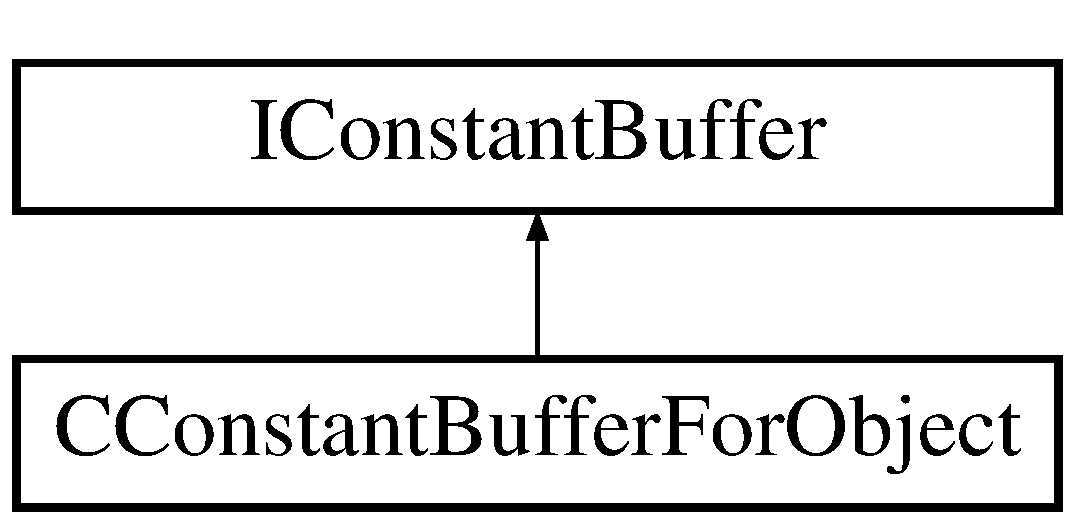
\includegraphics[height=2.000000cm]{class_c_constant_buffer_for_object}
\end{center}
\end{figure}
\subsection*{クラス}
\begin{DoxyCompactItemize}
\item 
struct \hyperlink{struct_c_constant_buffer_for_object_1_1_st_constant_buffer}{St\+Constant\+Buffer}
\begin{DoxyCompactList}\small\item\em コンスタントバッファー構造体。 \end{DoxyCompactList}\end{DoxyCompactItemize}
\subsection*{公開メンバ関数}
\begin{DoxyCompactItemize}
\item 
\hyperlink{class_c_constant_buffer_for_object_a41e7fd82a1adb51310d29dd16769d0a1}{C\+Constant\+Buffer\+For\+Object} ()
\begin{DoxyCompactList}\small\item\em コンストラクタ。 \end{DoxyCompactList}\item 
virtual \hyperlink{class_c_constant_buffer_for_object_a5249e7edc97e8f4fc901e880e2bd0059}{$\sim$\+C\+Constant\+Buffer\+For\+Object} ()
\begin{DoxyCompactList}\small\item\em デストラクタ。 \end{DoxyCompactList}\item 
virtual const void $\ast$ \hyperlink{class_c_constant_buffer_for_object_aa13289af40c27707fb174a5b3afbdf1b}{Get\+Data} () const  override
\begin{DoxyCompactList}\small\item\em データを取得。 \end{DoxyCompactList}\item 
virtual U\+Size \hyperlink{class_c_constant_buffer_for_object_a328586af4370d221ada7b270f9f4b8db}{Get\+Size} () const  override
\begin{DoxyCompactList}\small\item\em データサイズを取得。 \end{DoxyCompactList}\end{DoxyCompactItemize}
\subsection*{非公開変数類}
\begin{DoxyCompactItemize}
\item 
\hyperlink{struct_c_constant_buffer_for_object_1_1_st_constant_buffer}{St\+Constant\+Buffer} \hyperlink{class_c_constant_buffer_for_object_af80f6e3c636cac07ef26f291a005f979}{m\+\_\+st\+Buffer}
\end{DoxyCompactItemize}


\subsection{構築子と解体子}
\hypertarget{class_c_constant_buffer_for_object_a41e7fd82a1adb51310d29dd16769d0a1}{}\index{C\+Constant\+Buffer\+For\+Object@{C\+Constant\+Buffer\+For\+Object}!C\+Constant\+Buffer\+For\+Object@{C\+Constant\+Buffer\+For\+Object}}
\index{C\+Constant\+Buffer\+For\+Object@{C\+Constant\+Buffer\+For\+Object}!C\+Constant\+Buffer\+For\+Object@{C\+Constant\+Buffer\+For\+Object}}
\subsubsection[{C\+Constant\+Buffer\+For\+Object()}]{\setlength{\rightskip}{0pt plus 5cm}C\+Constant\+Buffer\+For\+Object\+::\+C\+Constant\+Buffer\+For\+Object (
\begin{DoxyParamCaption}
{}
\end{DoxyParamCaption}
)}\label{class_c_constant_buffer_for_object_a41e7fd82a1adb51310d29dd16769d0a1}


コンストラクタ。 

\hypertarget{class_c_constant_buffer_for_object_a5249e7edc97e8f4fc901e880e2bd0059}{}\index{C\+Constant\+Buffer\+For\+Object@{C\+Constant\+Buffer\+For\+Object}!````~C\+Constant\+Buffer\+For\+Object@{$\sim$\+C\+Constant\+Buffer\+For\+Object}}
\index{````~C\+Constant\+Buffer\+For\+Object@{$\sim$\+C\+Constant\+Buffer\+For\+Object}!C\+Constant\+Buffer\+For\+Object@{C\+Constant\+Buffer\+For\+Object}}
\subsubsection[{$\sim$\+C\+Constant\+Buffer\+For\+Object()}]{\setlength{\rightskip}{0pt plus 5cm}virtual C\+Constant\+Buffer\+For\+Object\+::$\sim$\+C\+Constant\+Buffer\+For\+Object (
\begin{DoxyParamCaption}
{}
\end{DoxyParamCaption}
)\hspace{0.3cm}{\ttfamily [inline]}, {\ttfamily [virtual]}}\label{class_c_constant_buffer_for_object_a5249e7edc97e8f4fc901e880e2bd0059}


デストラクタ。 



\subsection{関数詳解}
\hypertarget{class_c_constant_buffer_for_object_aa13289af40c27707fb174a5b3afbdf1b}{}\index{C\+Constant\+Buffer\+For\+Object@{C\+Constant\+Buffer\+For\+Object}!Get\+Data@{Get\+Data}}
\index{Get\+Data@{Get\+Data}!C\+Constant\+Buffer\+For\+Object@{C\+Constant\+Buffer\+For\+Object}}
\subsubsection[{Get\+Data() const  override}]{\setlength{\rightskip}{0pt plus 5cm}virtual const void$\ast$ C\+Constant\+Buffer\+For\+Object\+::\+Get\+Data (
\begin{DoxyParamCaption}
{}
\end{DoxyParamCaption}
) const\hspace{0.3cm}{\ttfamily [inline]}, {\ttfamily [override]}, {\ttfamily [virtual]}}\label{class_c_constant_buffer_for_object_aa13289af40c27707fb174a5b3afbdf1b}


データを取得。 



\hyperlink{class_i_constant_buffer_a51d7e72f262e74f2018b480102dc795e}{I\+Constant\+Buffer}を実装しています。

\hypertarget{class_c_constant_buffer_for_object_a328586af4370d221ada7b270f9f4b8db}{}\index{C\+Constant\+Buffer\+For\+Object@{C\+Constant\+Buffer\+For\+Object}!Get\+Size@{Get\+Size}}
\index{Get\+Size@{Get\+Size}!C\+Constant\+Buffer\+For\+Object@{C\+Constant\+Buffer\+For\+Object}}
\subsubsection[{Get\+Size() const  override}]{\setlength{\rightskip}{0pt plus 5cm}virtual U\+Size C\+Constant\+Buffer\+For\+Object\+::\+Get\+Size (
\begin{DoxyParamCaption}
{}
\end{DoxyParamCaption}
) const\hspace{0.3cm}{\ttfamily [inline]}, {\ttfamily [override]}, {\ttfamily [virtual]}}\label{class_c_constant_buffer_for_object_a328586af4370d221ada7b270f9f4b8db}


データサイズを取得。 



\hyperlink{class_i_constant_buffer_a527035ebacd73ffe5c5856f75220ac68}{I\+Constant\+Buffer}を実装しています。



\subsection{メンバ詳解}
\hypertarget{class_c_constant_buffer_for_object_af80f6e3c636cac07ef26f291a005f979}{}\index{C\+Constant\+Buffer\+For\+Object@{C\+Constant\+Buffer\+For\+Object}!m\+\_\+st\+Buffer@{m\+\_\+st\+Buffer}}
\index{m\+\_\+st\+Buffer@{m\+\_\+st\+Buffer}!C\+Constant\+Buffer\+For\+Object@{C\+Constant\+Buffer\+For\+Object}}
\subsubsection[{m\+\_\+st\+Buffer}]{\setlength{\rightskip}{0pt plus 5cm}{\bf St\+Constant\+Buffer} C\+Constant\+Buffer\+For\+Object\+::m\+\_\+st\+Buffer\hspace{0.3cm}{\ttfamily [private]}}\label{class_c_constant_buffer_for_object_af80f6e3c636cac07ef26f291a005f979}


このクラス詳解は次のファイルから抽出されました\+:\begin{DoxyCompactItemize}
\item 
D\+:/\+Project/\+Game/\+Lib/\+Render/\hyperlink{_constant_buffer_for_object_8h}{Constant\+Buffer\+For\+Object.\+h}\item 
D\+:/\+Project/\+Game/\+Lib/\+Math/\hyperlink{_constant_buffer_for_object_8cpp}{Constant\+Buffer\+For\+Object.\+cpp}\end{DoxyCompactItemize}

\hypertarget{class_c_critical_section}{}\section{C\+Critical\+Section クラス}
\label{class_c_critical_section}\index{C\+Critical\+Section@{C\+Critical\+Section}}


{\ttfamily \#include $<$Critical\+Section.\+h$>$}

\subsection*{公開メンバ関数}
\begin{DoxyCompactItemize}
\item 
\hyperlink{class_c_critical_section_ac72884ebdba4c5f3a19fd0fd2e88eff9}{C\+Critical\+Section} ()
\begin{DoxyCompactList}\small\item\em コンストラクタ。 \end{DoxyCompactList}\item 
virtual \hyperlink{class_c_critical_section_a60ef2d8b504bcca10bdcc485fe6dc3bb}{$\sim$\+C\+Critical\+Section} ()
\begin{DoxyCompactList}\small\item\em デストラクタ。 \end{DoxyCompactList}\item 
void \hyperlink{class_c_critical_section_a7234a370d8ba3cfee12b39b899e817fa}{Enter} ()
\begin{DoxyCompactList}\small\item\em クリティカルセクション開始。 \end{DoxyCompactList}\item 
void \hyperlink{class_c_critical_section_a6e60879511af2f366c1f41f06d8af9d5}{Leave} ()
\begin{DoxyCompactList}\small\item\em クリティカルセクション終了。 \end{DoxyCompactList}\end{DoxyCompactItemize}
\subsection*{非公開変数類}
\begin{DoxyCompactItemize}
\item 
C\+R\+I\+T\+I\+C\+A\+L\+\_\+\+S\+E\+C\+T\+I\+O\+N \hyperlink{class_c_critical_section_a803df161d876cc6566c3c6a07673c572}{m\+\_\+st\+Critical\+Section}
\end{DoxyCompactItemize}


\subsection{構築子と解体子}
\hypertarget{class_c_critical_section_ac72884ebdba4c5f3a19fd0fd2e88eff9}{}\index{C\+Critical\+Section@{C\+Critical\+Section}!C\+Critical\+Section@{C\+Critical\+Section}}
\index{C\+Critical\+Section@{C\+Critical\+Section}!C\+Critical\+Section@{C\+Critical\+Section}}
\subsubsection[{C\+Critical\+Section()}]{\setlength{\rightskip}{0pt plus 5cm}C\+Critical\+Section\+::\+C\+Critical\+Section (
\begin{DoxyParamCaption}
{}
\end{DoxyParamCaption}
)}\label{class_c_critical_section_ac72884ebdba4c5f3a19fd0fd2e88eff9}


コンストラクタ。 

\hypertarget{class_c_critical_section_a60ef2d8b504bcca10bdcc485fe6dc3bb}{}\index{C\+Critical\+Section@{C\+Critical\+Section}!````~C\+Critical\+Section@{$\sim$\+C\+Critical\+Section}}
\index{````~C\+Critical\+Section@{$\sim$\+C\+Critical\+Section}!C\+Critical\+Section@{C\+Critical\+Section}}
\subsubsection[{$\sim$\+C\+Critical\+Section()}]{\setlength{\rightskip}{0pt plus 5cm}C\+Critical\+Section\+::$\sim$\+C\+Critical\+Section (
\begin{DoxyParamCaption}
{}
\end{DoxyParamCaption}
)\hspace{0.3cm}{\ttfamily [virtual]}}\label{class_c_critical_section_a60ef2d8b504bcca10bdcc485fe6dc3bb}


デストラクタ。 



\subsection{関数詳解}
\hypertarget{class_c_critical_section_a7234a370d8ba3cfee12b39b899e817fa}{}\index{C\+Critical\+Section@{C\+Critical\+Section}!Enter@{Enter}}
\index{Enter@{Enter}!C\+Critical\+Section@{C\+Critical\+Section}}
\subsubsection[{Enter()}]{\setlength{\rightskip}{0pt plus 5cm}void C\+Critical\+Section\+::\+Enter (
\begin{DoxyParamCaption}
{}
\end{DoxyParamCaption}
)}\label{class_c_critical_section_a7234a370d8ba3cfee12b39b899e817fa}


クリティカルセクション開始。 

\hypertarget{class_c_critical_section_a6e60879511af2f366c1f41f06d8af9d5}{}\index{C\+Critical\+Section@{C\+Critical\+Section}!Leave@{Leave}}
\index{Leave@{Leave}!C\+Critical\+Section@{C\+Critical\+Section}}
\subsubsection[{Leave()}]{\setlength{\rightskip}{0pt plus 5cm}void C\+Critical\+Section\+::\+Leave (
\begin{DoxyParamCaption}
{}
\end{DoxyParamCaption}
)}\label{class_c_critical_section_a6e60879511af2f366c1f41f06d8af9d5}


クリティカルセクション終了。 



\subsection{メンバ詳解}
\hypertarget{class_c_critical_section_a803df161d876cc6566c3c6a07673c572}{}\index{C\+Critical\+Section@{C\+Critical\+Section}!m\+\_\+st\+Critical\+Section@{m\+\_\+st\+Critical\+Section}}
\index{m\+\_\+st\+Critical\+Section@{m\+\_\+st\+Critical\+Section}!C\+Critical\+Section@{C\+Critical\+Section}}
\subsubsection[{m\+\_\+st\+Critical\+Section}]{\setlength{\rightskip}{0pt plus 5cm}C\+R\+I\+T\+I\+C\+A\+L\+\_\+\+S\+E\+C\+T\+I\+O\+N C\+Critical\+Section\+::m\+\_\+st\+Critical\+Section\hspace{0.3cm}{\ttfamily [private]}}\label{class_c_critical_section_a803df161d876cc6566c3c6a07673c572}


このクラス詳解は次のファイルから抽出されました\+:\begin{DoxyCompactItemize}
\item 
D\+:/\+Project/\+Game/\+Lib/\+Thread/\hyperlink{_critical_section_8h}{Critical\+Section.\+h}\item 
D\+:/\+Project/\+Game/\+Lib/\+Thread/\hyperlink{_critical_section_8cpp}{Critical\+Section.\+cpp}\end{DoxyCompactItemize}

\hypertarget{class_c_critical_section_block}{}\section{C\+Critical\+Section\+Block クラス}
\label{class_c_critical_section_block}\index{C\+Critical\+Section\+Block@{C\+Critical\+Section\+Block}}


{\ttfamily \#include $<$Critical\+Section.\+h$>$}

\subsection*{公開メンバ関数}
\begin{DoxyCompactItemize}
\item 
\hyperlink{class_c_critical_section_block_a295a4d00010754caa3c188859869e157}{C\+Critical\+Section\+Block} (\hyperlink{class_c_critical_section}{C\+Critical\+Section} $\ast$\+\_\+pc\+Critical\+Section)
\begin{DoxyCompactList}\small\item\em コンストラクタ。 \end{DoxyCompactList}\item 
virtual \hyperlink{class_c_critical_section_block_a006b2ae6888c906d95fead637992331c}{$\sim$\+C\+Critical\+Section\+Block} ()
\begin{DoxyCompactList}\small\item\em デストラクタ。 \end{DoxyCompactList}\end{DoxyCompactItemize}
\subsection*{非公開変数類}
\begin{DoxyCompactItemize}
\item 
\hyperlink{class_c_critical_section}{C\+Critical\+Section} $\ast$ \hyperlink{class_c_critical_section_block_a85e6abc3f5091afdc7f8127737885974}{m\+\_\+pc\+Critical\+Section}
\end{DoxyCompactItemize}


\subsection{構築子と解体子}
\hypertarget{class_c_critical_section_block_a295a4d00010754caa3c188859869e157}{}\index{C\+Critical\+Section\+Block@{C\+Critical\+Section\+Block}!C\+Critical\+Section\+Block@{C\+Critical\+Section\+Block}}
\index{C\+Critical\+Section\+Block@{C\+Critical\+Section\+Block}!C\+Critical\+Section\+Block@{C\+Critical\+Section\+Block}}
\subsubsection[{C\+Critical\+Section\+Block(\+C\+Critical\+Section $\ast$\+\_\+pc\+Critical\+Section)}]{\setlength{\rightskip}{0pt plus 5cm}C\+Critical\+Section\+Block\+::\+C\+Critical\+Section\+Block (
\begin{DoxyParamCaption}
\item[{{\bf C\+Critical\+Section} $\ast$}]{\+\_\+pc\+Critical\+Section}
\end{DoxyParamCaption}
)}\label{class_c_critical_section_block_a295a4d00010754caa3c188859869e157}


コンストラクタ。 


\begin{DoxyParams}[1]{引数}
\mbox{\tt in}  & {\em \+\_\+pc\+Critical\+Section} & \+: クリティカルセクション。 \\
\hline
\end{DoxyParams}
\hypertarget{class_c_critical_section_block_a006b2ae6888c906d95fead637992331c}{}\index{C\+Critical\+Section\+Block@{C\+Critical\+Section\+Block}!````~C\+Critical\+Section\+Block@{$\sim$\+C\+Critical\+Section\+Block}}
\index{````~C\+Critical\+Section\+Block@{$\sim$\+C\+Critical\+Section\+Block}!C\+Critical\+Section\+Block@{C\+Critical\+Section\+Block}}
\subsubsection[{$\sim$\+C\+Critical\+Section\+Block()}]{\setlength{\rightskip}{0pt plus 5cm}C\+Critical\+Section\+Block\+::$\sim$\+C\+Critical\+Section\+Block (
\begin{DoxyParamCaption}
{}
\end{DoxyParamCaption}
)\hspace{0.3cm}{\ttfamily [virtual]}}\label{class_c_critical_section_block_a006b2ae6888c906d95fead637992331c}


デストラクタ。 



\subsection{メンバ詳解}
\hypertarget{class_c_critical_section_block_a85e6abc3f5091afdc7f8127737885974}{}\index{C\+Critical\+Section\+Block@{C\+Critical\+Section\+Block}!m\+\_\+pc\+Critical\+Section@{m\+\_\+pc\+Critical\+Section}}
\index{m\+\_\+pc\+Critical\+Section@{m\+\_\+pc\+Critical\+Section}!C\+Critical\+Section\+Block@{C\+Critical\+Section\+Block}}
\subsubsection[{m\+\_\+pc\+Critical\+Section}]{\setlength{\rightskip}{0pt plus 5cm}{\bf C\+Critical\+Section}$\ast$ C\+Critical\+Section\+Block\+::m\+\_\+pc\+Critical\+Section\hspace{0.3cm}{\ttfamily [private]}}\label{class_c_critical_section_block_a85e6abc3f5091afdc7f8127737885974}


このクラス詳解は次のファイルから抽出されました\+:\begin{DoxyCompactItemize}
\item 
D\+:/\+Project/\+Game/\+Lib/\+Thread/\hyperlink{_critical_section_8h}{Critical\+Section.\+h}\item 
D\+:/\+Project/\+Game/\+Lib/\+Thread/\hyperlink{_critical_section_8cpp}{Critical\+Section.\+cpp}\end{DoxyCompactItemize}

\hypertarget{class_c_debug_process_time}{}\section{C\+Debug\+Process\+Time クラス}
\label{class_c_debug_process_time}\index{C\+Debug\+Process\+Time@{C\+Debug\+Process\+Time}}


{\ttfamily \#include $<$Debug\+Process\+Time.\+h$>$}

\subsection*{公開メンバ関数}
\begin{DoxyCompactItemize}
\item 
\hyperlink{class_c_debug_process_time_acfd9d897cfacd9c37f1b95921052c4d7}{C\+Debug\+Process\+Time} (const S8 $\ast$\+\_\+ps\+Function)
\item 
\hyperlink{class_c_debug_process_time_a39ccc95264adb9a18093b20dfc34f2c7}{$\sim$\+C\+Debug\+Process\+Time} ()
\item 
void \hyperlink{class_c_debug_process_time_af324f580c88fc3ee4e3e953916bc6835}{Reset} ()
\item 
U64 \hyperlink{class_c_debug_process_time_a888bf783d5d5a25517ef29fc6bb13b87}{Get\+Process\+Time} () const 
\end{DoxyCompactItemize}
\subsection*{非公開変数類}
\begin{DoxyCompactItemize}
\item 
const S8 $\ast$ \hyperlink{class_c_debug_process_time_ae749da6a0425559cc94c16b0539eb0db}{m\+\_\+ps\+Function}
\item 
U64 \hyperlink{class_c_debug_process_time_ae521d38084feca1cbd666964c50113a2}{m\+\_\+u\+Start\+Time}
\end{DoxyCompactItemize}


\subsection{構築子と解体子}
\hypertarget{class_c_debug_process_time_acfd9d897cfacd9c37f1b95921052c4d7}{}\index{C\+Debug\+Process\+Time@{C\+Debug\+Process\+Time}!C\+Debug\+Process\+Time@{C\+Debug\+Process\+Time}}
\index{C\+Debug\+Process\+Time@{C\+Debug\+Process\+Time}!C\+Debug\+Process\+Time@{C\+Debug\+Process\+Time}}
\subsubsection[{C\+Debug\+Process\+Time(const S8 $\ast$\+\_\+ps\+Function)}]{\setlength{\rightskip}{0pt plus 5cm}C\+Debug\+Process\+Time\+::\+C\+Debug\+Process\+Time (
\begin{DoxyParamCaption}
\item[{const S8 $\ast$}]{\+\_\+ps\+Function}
\end{DoxyParamCaption}
)}\label{class_c_debug_process_time_acfd9d897cfacd9c37f1b95921052c4d7}
\hypertarget{class_c_debug_process_time_a39ccc95264adb9a18093b20dfc34f2c7}{}\index{C\+Debug\+Process\+Time@{C\+Debug\+Process\+Time}!````~C\+Debug\+Process\+Time@{$\sim$\+C\+Debug\+Process\+Time}}
\index{````~C\+Debug\+Process\+Time@{$\sim$\+C\+Debug\+Process\+Time}!C\+Debug\+Process\+Time@{C\+Debug\+Process\+Time}}
\subsubsection[{$\sim$\+C\+Debug\+Process\+Time()}]{\setlength{\rightskip}{0pt plus 5cm}C\+Debug\+Process\+Time\+::$\sim$\+C\+Debug\+Process\+Time (
\begin{DoxyParamCaption}
{}
\end{DoxyParamCaption}
)}\label{class_c_debug_process_time_a39ccc95264adb9a18093b20dfc34f2c7}


\subsection{関数詳解}
\hypertarget{class_c_debug_process_time_a888bf783d5d5a25517ef29fc6bb13b87}{}\index{C\+Debug\+Process\+Time@{C\+Debug\+Process\+Time}!Get\+Process\+Time@{Get\+Process\+Time}}
\index{Get\+Process\+Time@{Get\+Process\+Time}!C\+Debug\+Process\+Time@{C\+Debug\+Process\+Time}}
\subsubsection[{Get\+Process\+Time() const }]{\setlength{\rightskip}{0pt plus 5cm}U64 C\+Debug\+Process\+Time\+::\+Get\+Process\+Time (
\begin{DoxyParamCaption}
{}
\end{DoxyParamCaption}
) const}\label{class_c_debug_process_time_a888bf783d5d5a25517ef29fc6bb13b87}
\hypertarget{class_c_debug_process_time_af324f580c88fc3ee4e3e953916bc6835}{}\index{C\+Debug\+Process\+Time@{C\+Debug\+Process\+Time}!Reset@{Reset}}
\index{Reset@{Reset}!C\+Debug\+Process\+Time@{C\+Debug\+Process\+Time}}
\subsubsection[{Reset()}]{\setlength{\rightskip}{0pt plus 5cm}void C\+Debug\+Process\+Time\+::\+Reset (
\begin{DoxyParamCaption}
{}
\end{DoxyParamCaption}
)}\label{class_c_debug_process_time_af324f580c88fc3ee4e3e953916bc6835}


\subsection{メンバ詳解}
\hypertarget{class_c_debug_process_time_ae749da6a0425559cc94c16b0539eb0db}{}\index{C\+Debug\+Process\+Time@{C\+Debug\+Process\+Time}!m\+\_\+ps\+Function@{m\+\_\+ps\+Function}}
\index{m\+\_\+ps\+Function@{m\+\_\+ps\+Function}!C\+Debug\+Process\+Time@{C\+Debug\+Process\+Time}}
\subsubsection[{m\+\_\+ps\+Function}]{\setlength{\rightskip}{0pt plus 5cm}const S8$\ast$ C\+Debug\+Process\+Time\+::m\+\_\+ps\+Function\hspace{0.3cm}{\ttfamily [private]}}\label{class_c_debug_process_time_ae749da6a0425559cc94c16b0539eb0db}
\hypertarget{class_c_debug_process_time_ae521d38084feca1cbd666964c50113a2}{}\index{C\+Debug\+Process\+Time@{C\+Debug\+Process\+Time}!m\+\_\+u\+Start\+Time@{m\+\_\+u\+Start\+Time}}
\index{m\+\_\+u\+Start\+Time@{m\+\_\+u\+Start\+Time}!C\+Debug\+Process\+Time@{C\+Debug\+Process\+Time}}
\subsubsection[{m\+\_\+u\+Start\+Time}]{\setlength{\rightskip}{0pt plus 5cm}U64 C\+Debug\+Process\+Time\+::m\+\_\+u\+Start\+Time\hspace{0.3cm}{\ttfamily [private]}}\label{class_c_debug_process_time_ae521d38084feca1cbd666964c50113a2}


このクラス詳解は次のファイルから抽出されました\+:\begin{DoxyCompactItemize}
\item 
D\+:/\+Project/\+Game/\+Lib/\+Debug/\hyperlink{_debug_process_time_8h}{Debug\+Process\+Time.\+h}\item 
D\+:/\+Project/\+Game/\+Lib/\+Debug/\hyperlink{_debug_process_time_8cpp}{Debug\+Process\+Time.\+cpp}\end{DoxyCompactItemize}

\hypertarget{class_c_direct_x}{}\section{C\+Direct\+X クラス}
\label{class_c_direct_x}\index{C\+Direct\+X@{C\+Direct\+X}}


{\ttfamily \#include $<$Direct\+X.\+h$>$}

C\+Direct\+X の継承関係図\begin{figure}[H]
\begin{center}
\leavevmode
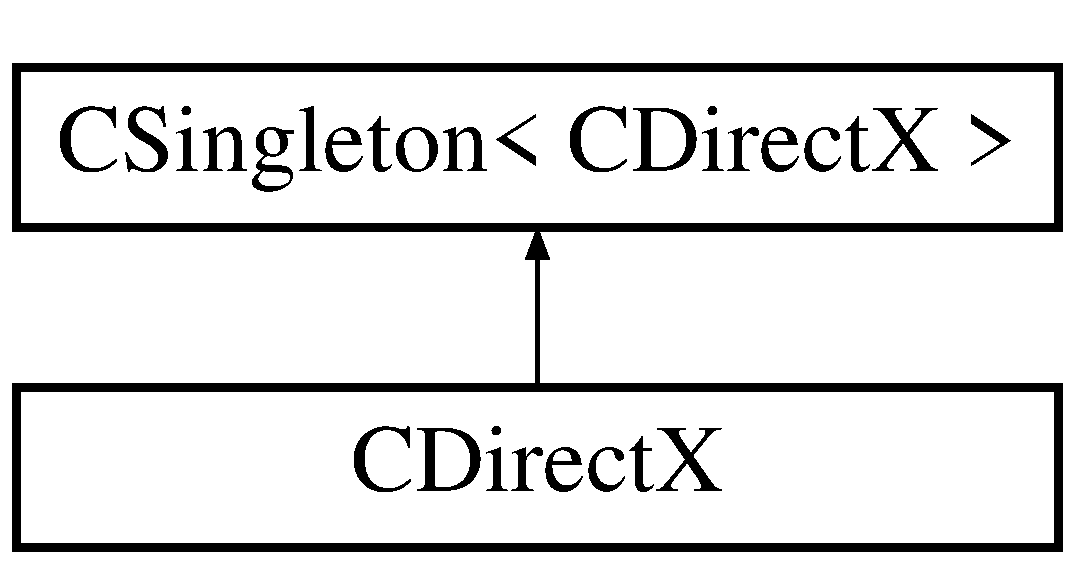
\includegraphics[height=2.000000cm]{class_c_direct_x}
\end{center}
\end{figure}
\subsection*{公開メンバ関数}
\begin{DoxyCompactItemize}
\item 
virtual \hyperlink{class_c_direct_x_a59b5bb11e5e08ccc56e89197b01fc868}{$\sim$\+C\+Direct\+X} ()
\begin{DoxyCompactList}\small\item\em デストラクタ。 \end{DoxyCompactList}\item 
void \hyperlink{class_c_direct_x_ae32df5ee0af2d29f4ba27e95935e0f10}{Init} (\hyperlink{class_i_direct_x_device_factory}{I\+Direct\+X\+Device\+Factory} $\ast$\+\_\+pc\+Factory)
\begin{DoxyCompactList}\small\item\em 初期化。 \end{DoxyCompactList}\end{DoxyCompactItemize}
\subsection*{静的公開メンバ関数}
\begin{DoxyCompactItemize}
\item 
static I\+D3\+D\+Device $\ast$ \hyperlink{class_c_direct_x_a55ff92addc24828d45a9915b756cd0f1}{Get\+Device} ()
\begin{DoxyCompactList}\small\item\em デバイスを取得。 \end{DoxyCompactList}\end{DoxyCompactItemize}
\subsection*{非公開メンバ関数}
\begin{DoxyCompactItemize}
\item 
\hyperlink{class_c_direct_x_a2653832713605e020f84920299c17ff3}{C\+Direct\+X} ()
\begin{DoxyCompactList}\small\item\em コンストラクタ。 \end{DoxyCompactList}\end{DoxyCompactItemize}
\subsection*{非公開変数類}
\begin{DoxyCompactItemize}
\item 
friend \hyperlink{class_c_direct_x_a7c51dd8b68b56ffa5bed852e4dd13a92}{C\+Singleton$<$ C\+Direct\+X $>$}
\item 
I\+D3\+D\+Device $\ast$ \hyperlink{class_c_direct_x_a6ecdada46fbabcb5535cede3a96fdbe3}{m\+\_\+pc\+Device}
\end{DoxyCompactItemize}
\subsection*{その他の継承メンバ}


\subsection{構築子と解体子}
\hypertarget{class_c_direct_x_a2653832713605e020f84920299c17ff3}{}\index{C\+Direct\+X@{C\+Direct\+X}!C\+Direct\+X@{C\+Direct\+X}}
\index{C\+Direct\+X@{C\+Direct\+X}!C\+Direct\+X@{C\+Direct\+X}}
\subsubsection[{C\+Direct\+X()}]{\setlength{\rightskip}{0pt plus 5cm}C\+Direct\+X\+::\+C\+Direct\+X (
\begin{DoxyParamCaption}
{}
\end{DoxyParamCaption}
)\hspace{0.3cm}{\ttfamily [private]}}\label{class_c_direct_x_a2653832713605e020f84920299c17ff3}


コンストラクタ。 

\hypertarget{class_c_direct_x_a59b5bb11e5e08ccc56e89197b01fc868}{}\index{C\+Direct\+X@{C\+Direct\+X}!````~C\+Direct\+X@{$\sim$\+C\+Direct\+X}}
\index{````~C\+Direct\+X@{$\sim$\+C\+Direct\+X}!C\+Direct\+X@{C\+Direct\+X}}
\subsubsection[{$\sim$\+C\+Direct\+X()}]{\setlength{\rightskip}{0pt plus 5cm}C\+Direct\+X\+::$\sim$\+C\+Direct\+X (
\begin{DoxyParamCaption}
{}
\end{DoxyParamCaption}
)\hspace{0.3cm}{\ttfamily [virtual]}}\label{class_c_direct_x_a59b5bb11e5e08ccc56e89197b01fc868}


デストラクタ。 



\subsection{関数詳解}
\hypertarget{class_c_direct_x_a55ff92addc24828d45a9915b756cd0f1}{}\index{C\+Direct\+X@{C\+Direct\+X}!Get\+Device@{Get\+Device}}
\index{Get\+Device@{Get\+Device}!C\+Direct\+X@{C\+Direct\+X}}
\subsubsection[{Get\+Device()}]{\setlength{\rightskip}{0pt plus 5cm}I\+D3\+D\+Device $\ast$ C\+Direct\+X\+::\+Get\+Device (
\begin{DoxyParamCaption}
{}
\end{DoxyParamCaption}
)\hspace{0.3cm}{\ttfamily [static]}}\label{class_c_direct_x_a55ff92addc24828d45a9915b756cd0f1}


デバイスを取得。 


\begin{DoxyRetVals}{戻り値}
{\em I\+D3\+D\+Device$\ast$} & \+: Direct\+X\+Device。 \\
\hline
\end{DoxyRetVals}
\hypertarget{class_c_direct_x_ae32df5ee0af2d29f4ba27e95935e0f10}{}\index{C\+Direct\+X@{C\+Direct\+X}!Init@{Init}}
\index{Init@{Init}!C\+Direct\+X@{C\+Direct\+X}}
\subsubsection[{Init(\+I\+Direct\+X\+Device\+Factory $\ast$\+\_\+pc\+Factory)}]{\setlength{\rightskip}{0pt plus 5cm}void C\+Direct\+X\+::\+Init (
\begin{DoxyParamCaption}
\item[{{\bf I\+Direct\+X\+Device\+Factory} $\ast$}]{\+\_\+pc\+Factory}
\end{DoxyParamCaption}
)}\label{class_c_direct_x_ae32df5ee0af2d29f4ba27e95935e0f10}


初期化。 


\begin{DoxyParams}[1]{引数}
\mbox{\tt in}  & {\em \+\_\+pc\+Factory} & \+: デバイス生成クラス。 \\
\hline
\end{DoxyParams}


\subsection{メンバ詳解}
\hypertarget{class_c_direct_x_a7c51dd8b68b56ffa5bed852e4dd13a92}{}\index{C\+Direct\+X@{C\+Direct\+X}!C\+Singleton$<$ C\+Direct\+X $>$@{C\+Singleton$<$ C\+Direct\+X $>$}}
\index{C\+Singleton$<$ C\+Direct\+X $>$@{C\+Singleton$<$ C\+Direct\+X $>$}!C\+Direct\+X@{C\+Direct\+X}}
\subsubsection[{C\+Singleton$<$ C\+Direct\+X $>$}]{\setlength{\rightskip}{0pt plus 5cm}friend {\bf C\+Direct\+X\+::\+C\+Singleton}$<$ {\bf C\+Direct\+X} $>$\hspace{0.3cm}{\ttfamily [private]}}\label{class_c_direct_x_a7c51dd8b68b56ffa5bed852e4dd13a92}
\hypertarget{class_c_direct_x_a6ecdada46fbabcb5535cede3a96fdbe3}{}\index{C\+Direct\+X@{C\+Direct\+X}!m\+\_\+pc\+Device@{m\+\_\+pc\+Device}}
\index{m\+\_\+pc\+Device@{m\+\_\+pc\+Device}!C\+Direct\+X@{C\+Direct\+X}}
\subsubsection[{m\+\_\+pc\+Device}]{\setlength{\rightskip}{0pt plus 5cm}I\+D3\+D\+Device$\ast$ C\+Direct\+X\+::m\+\_\+pc\+Device\hspace{0.3cm}{\ttfamily [private]}}\label{class_c_direct_x_a6ecdada46fbabcb5535cede3a96fdbe3}


このクラス詳解は次のファイルから抽出されました\+:\begin{DoxyCompactItemize}
\item 
D\+:/\+Project/\+Game/\+Lib/\+Direct\+X/\hyperlink{_direct_x_8h}{Direct\+X.\+h}\item 
D\+:/\+Project/\+Game/\+Lib/\+Direct\+X/\hyperlink{_direct_x_8cpp}{Direct\+X.\+cpp}\end{DoxyCompactItemize}

\hypertarget{class_c_direct_x_shader_manager}{}\section{C\+Direct\+X\+Shader\+Manager クラス}
\label{class_c_direct_x_shader_manager}\index{C\+Direct\+X\+Shader\+Manager@{C\+Direct\+X\+Shader\+Manager}}


{\ttfamily \#include $<$Direct\+X\+Shader\+Manager.\+h$>$}

\subsection*{公開メンバ関数}
\begin{DoxyCompactItemize}
\item 
\hyperlink{class_c_direct_x_shader_manager_a40710f22f33988c7ee6b2d0846738e46}{C\+Direct\+X\+Shader\+Manager} ()
\begin{DoxyCompactList}\small\item\em コンストラクタ。 \end{DoxyCompactList}\item 
virtual \hyperlink{class_c_direct_x_shader_manager_ad54969294f58847ac0bb1d91eabf7978}{$\sim$\+C\+Direct\+X\+Shader\+Manager} ()
\begin{DoxyCompactList}\small\item\em デストラクタ。 \end{DoxyCompactList}\item 
const \hyperlink{class_c_vertex_shader}{C\+Vertex\+Shader} $\ast$ \hyperlink{class_c_direct_x_shader_manager_abf4e16c5b7fca6755d01d1a1e4f7b623}{Get\+Vertex\+Shader} (\hyperlink{_shader_definition_8h_a232ca48c9a8e2a62b45a96e7929a2bdb}{En\+Vertex\+Shader} \+\_\+e\+Vertex\+Shader) const 
\begin{DoxyCompactList}\small\item\em 頂点シェーダーを取得。 \end{DoxyCompactList}\item 
const \hyperlink{class_c_pixel_shader}{C\+Pixel\+Shader} $\ast$ \hyperlink{class_c_direct_x_shader_manager_a04f2e46307dac941beffb075dc4f21e9}{Get\+Pixel\+Shader} (\hyperlink{_shader_definition_8h_ab8ae26d268e6e5baee47fbba4d03f4cf}{En\+Pixel\+Shader} \+\_\+e\+Pixel\+Shader) const 
\begin{DoxyCompactList}\small\item\em ピクセルシェーダーを取得。 \end{DoxyCompactList}\item 
bool \hyperlink{class_c_direct_x_shader_manager_a3099819b5ea0631e419485554d4e1095}{Is\+Read\+End} () const 
\begin{DoxyCompactList}\small\item\em 読み込みが完了したか。 \end{DoxyCompactList}\end{DoxyCompactItemize}
\subsection*{非公開変数類}
\begin{DoxyCompactItemize}
\item 
\hyperlink{class_c_vertex_shader}{C\+Vertex\+Shader} $\ast$ \hyperlink{class_c_direct_x_shader_manager_ac5f58343fb18d284ddd799f5728d29aa}{m\+\_\+pc\+Vertex\+Shader\+Array} \mbox{[}\hyperlink{_lib_utility_8h_a564389767079011d2a47cdb641d81353}{s\+\_\+cast}$<$ U32 $>$(\hyperlink{_shader_definition_8h_a232ca48c9a8e2a62b45a96e7929a2bdba079bb6413c37006b9fdc56add34e517b}{En\+Vertex\+Shader\+::en\+Max})\mbox{]}
\item 
\hyperlink{class_c_pixel_shader}{C\+Pixel\+Shader} $\ast$ \hyperlink{class_c_direct_x_shader_manager_a2f6249831a45357aaa133c615603a54b}{m\+\_\+pc\+Pixel\+Shader\+Array} \mbox{[}\hyperlink{_lib_utility_8h_a564389767079011d2a47cdb641d81353}{s\+\_\+cast}$<$ U32 $>$(\hyperlink{_shader_definition_8h_ab8ae26d268e6e5baee47fbba4d03f4cfa079bb6413c37006b9fdc56add34e517b}{En\+Pixel\+Shader\+::en\+Max})\mbox{]}
\end{DoxyCompactItemize}


\subsection{構築子と解体子}
\hypertarget{class_c_direct_x_shader_manager_a40710f22f33988c7ee6b2d0846738e46}{}\index{C\+Direct\+X\+Shader\+Manager@{C\+Direct\+X\+Shader\+Manager}!C\+Direct\+X\+Shader\+Manager@{C\+Direct\+X\+Shader\+Manager}}
\index{C\+Direct\+X\+Shader\+Manager@{C\+Direct\+X\+Shader\+Manager}!C\+Direct\+X\+Shader\+Manager@{C\+Direct\+X\+Shader\+Manager}}
\subsubsection[{C\+Direct\+X\+Shader\+Manager()}]{\setlength{\rightskip}{0pt plus 5cm}C\+Direct\+X\+Shader\+Manager\+::\+C\+Direct\+X\+Shader\+Manager (
\begin{DoxyParamCaption}
{}
\end{DoxyParamCaption}
)}\label{class_c_direct_x_shader_manager_a40710f22f33988c7ee6b2d0846738e46}


コンストラクタ。 

\hypertarget{class_c_direct_x_shader_manager_ad54969294f58847ac0bb1d91eabf7978}{}\index{C\+Direct\+X\+Shader\+Manager@{C\+Direct\+X\+Shader\+Manager}!````~C\+Direct\+X\+Shader\+Manager@{$\sim$\+C\+Direct\+X\+Shader\+Manager}}
\index{````~C\+Direct\+X\+Shader\+Manager@{$\sim$\+C\+Direct\+X\+Shader\+Manager}!C\+Direct\+X\+Shader\+Manager@{C\+Direct\+X\+Shader\+Manager}}
\subsubsection[{$\sim$\+C\+Direct\+X\+Shader\+Manager()}]{\setlength{\rightskip}{0pt plus 5cm}C\+Direct\+X\+Shader\+Manager\+::$\sim$\+C\+Direct\+X\+Shader\+Manager (
\begin{DoxyParamCaption}
{}
\end{DoxyParamCaption}
)\hspace{0.3cm}{\ttfamily [virtual]}}\label{class_c_direct_x_shader_manager_ad54969294f58847ac0bb1d91eabf7978}


デストラクタ。 



\subsection{関数詳解}
\hypertarget{class_c_direct_x_shader_manager_a04f2e46307dac941beffb075dc4f21e9}{}\index{C\+Direct\+X\+Shader\+Manager@{C\+Direct\+X\+Shader\+Manager}!Get\+Pixel\+Shader@{Get\+Pixel\+Shader}}
\index{Get\+Pixel\+Shader@{Get\+Pixel\+Shader}!C\+Direct\+X\+Shader\+Manager@{C\+Direct\+X\+Shader\+Manager}}
\subsubsection[{Get\+Pixel\+Shader(\+En\+Pixel\+Shader \+\_\+e\+Pixel\+Shader) const }]{\setlength{\rightskip}{0pt plus 5cm}const {\bf C\+Pixel\+Shader} $\ast$ C\+Direct\+X\+Shader\+Manager\+::\+Get\+Pixel\+Shader (
\begin{DoxyParamCaption}
\item[{{\bf En\+Pixel\+Shader}}]{\+\_\+e\+Pixel\+Shader}
\end{DoxyParamCaption}
) const}\label{class_c_direct_x_shader_manager_a04f2e46307dac941beffb075dc4f21e9}


ピクセルシェーダーを取得。 


\begin{DoxyParams}[1]{引数}
\mbox{\tt in}  & {\em \+\_\+e\+Pixel\+Shader} & \+: 取得するピクセルシェーダー。 \\
\hline
\end{DoxyParams}

\begin{DoxyRetVals}{戻り値}
{\em const} & C\+Pixel\+Shader$\ast$ \+: ピクセルシェーダー。 \\
\hline
\end{DoxyRetVals}
\hypertarget{class_c_direct_x_shader_manager_abf4e16c5b7fca6755d01d1a1e4f7b623}{}\index{C\+Direct\+X\+Shader\+Manager@{C\+Direct\+X\+Shader\+Manager}!Get\+Vertex\+Shader@{Get\+Vertex\+Shader}}
\index{Get\+Vertex\+Shader@{Get\+Vertex\+Shader}!C\+Direct\+X\+Shader\+Manager@{C\+Direct\+X\+Shader\+Manager}}
\subsubsection[{Get\+Vertex\+Shader(\+En\+Vertex\+Shader \+\_\+e\+Vertex\+Shader) const }]{\setlength{\rightskip}{0pt plus 5cm}const {\bf C\+Vertex\+Shader} $\ast$ C\+Direct\+X\+Shader\+Manager\+::\+Get\+Vertex\+Shader (
\begin{DoxyParamCaption}
\item[{{\bf En\+Vertex\+Shader}}]{\+\_\+e\+Vertex\+Shader}
\end{DoxyParamCaption}
) const}\label{class_c_direct_x_shader_manager_abf4e16c5b7fca6755d01d1a1e4f7b623}


頂点シェーダーを取得。 


\begin{DoxyParams}[1]{引数}
\mbox{\tt in}  & {\em \+\_\+e\+Vertex\+Shader} & \+: 取得する頂点シェーダー。 \\
\hline
\end{DoxyParams}

\begin{DoxyRetVals}{戻り値}
{\em const} & C\+Vertex\+Shader$\ast$ \+: 頂点シェーダー。 \\
\hline
\end{DoxyRetVals}
\hypertarget{class_c_direct_x_shader_manager_a3099819b5ea0631e419485554d4e1095}{}\index{C\+Direct\+X\+Shader\+Manager@{C\+Direct\+X\+Shader\+Manager}!Is\+Read\+End@{Is\+Read\+End}}
\index{Is\+Read\+End@{Is\+Read\+End}!C\+Direct\+X\+Shader\+Manager@{C\+Direct\+X\+Shader\+Manager}}
\subsubsection[{Is\+Read\+End() const }]{\setlength{\rightskip}{0pt plus 5cm}bool C\+Direct\+X\+Shader\+Manager\+::\+Is\+Read\+End (
\begin{DoxyParamCaption}
{}
\end{DoxyParamCaption}
) const}\label{class_c_direct_x_shader_manager_a3099819b5ea0631e419485554d4e1095}


読み込みが完了したか。 


\begin{DoxyRetVals}{戻り値}
{\em bool} & \+: 全てのシェーダーが使用可能になればtrue。 \\
\hline
\end{DoxyRetVals}


\subsection{メンバ詳解}
\hypertarget{class_c_direct_x_shader_manager_a2f6249831a45357aaa133c615603a54b}{}\index{C\+Direct\+X\+Shader\+Manager@{C\+Direct\+X\+Shader\+Manager}!m\+\_\+pc\+Pixel\+Shader\+Array@{m\+\_\+pc\+Pixel\+Shader\+Array}}
\index{m\+\_\+pc\+Pixel\+Shader\+Array@{m\+\_\+pc\+Pixel\+Shader\+Array}!C\+Direct\+X\+Shader\+Manager@{C\+Direct\+X\+Shader\+Manager}}
\subsubsection[{m\+\_\+pc\+Pixel\+Shader\+Array}]{\setlength{\rightskip}{0pt plus 5cm}{\bf C\+Pixel\+Shader}$\ast$ C\+Direct\+X\+Shader\+Manager\+::m\+\_\+pc\+Pixel\+Shader\+Array\mbox{[}{\bf s\+\_\+cast}$<$ U32 $>$({\bf En\+Pixel\+Shader\+::en\+Max})\mbox{]}\hspace{0.3cm}{\ttfamily [private]}}\label{class_c_direct_x_shader_manager_a2f6249831a45357aaa133c615603a54b}
\hypertarget{class_c_direct_x_shader_manager_ac5f58343fb18d284ddd799f5728d29aa}{}\index{C\+Direct\+X\+Shader\+Manager@{C\+Direct\+X\+Shader\+Manager}!m\+\_\+pc\+Vertex\+Shader\+Array@{m\+\_\+pc\+Vertex\+Shader\+Array}}
\index{m\+\_\+pc\+Vertex\+Shader\+Array@{m\+\_\+pc\+Vertex\+Shader\+Array}!C\+Direct\+X\+Shader\+Manager@{C\+Direct\+X\+Shader\+Manager}}
\subsubsection[{m\+\_\+pc\+Vertex\+Shader\+Array}]{\setlength{\rightskip}{0pt plus 5cm}{\bf C\+Vertex\+Shader}$\ast$ C\+Direct\+X\+Shader\+Manager\+::m\+\_\+pc\+Vertex\+Shader\+Array\mbox{[}{\bf s\+\_\+cast}$<$ U32 $>$({\bf En\+Vertex\+Shader\+::en\+Max})\mbox{]}\hspace{0.3cm}{\ttfamily [private]}}\label{class_c_direct_x_shader_manager_ac5f58343fb18d284ddd799f5728d29aa}


このクラス詳解は次のファイルから抽出されました\+:\begin{DoxyCompactItemize}
\item 
D\+:/\+Project/\+Game/\+Lib/\+Direct\+X/\hyperlink{_direct_x_shader_manager_8h}{Direct\+X\+Shader\+Manager.\+h}\item 
D\+:/\+Project/\+Game/\+Lib/\+Direct\+X/\hyperlink{_direct_x_shader_manager_8cpp}{Direct\+X\+Shader\+Manager.\+cpp}\end{DoxyCompactItemize}

\hypertarget{class_c_direct_x_texture}{}\section{C\+Direct\+X\+Texture クラス}
\label{class_c_direct_x_texture}\index{C\+Direct\+X\+Texture@{C\+Direct\+X\+Texture}}


{\ttfamily \#include $<$Direct\+X\+Texture.\+h$>$}

\subsection*{公開メンバ関数}
\begin{DoxyCompactItemize}
\item 
\hyperlink{class_c_direct_x_texture_a23305fa228b1ed1d3071b1cccae38d3c}{C\+Direct\+X\+Texture} ()
\begin{DoxyCompactList}\small\item\em コンストラクタ。 \end{DoxyCompactList}\item 
virtual \hyperlink{class_c_direct_x_texture_afd62064ff20750c1cc1dfd900ffac90c}{$\sim$\+C\+Direct\+X\+Texture} ()
\begin{DoxyCompactList}\small\item\em デストラクタ。 \end{DoxyCompactList}\item 
void \hyperlink{class_c_direct_x_texture_a544fd8fb0c2f2b26853f4930764da184}{Create\+Texture} (const D3\+D\+\_\+\+T\+E\+X\+T\+U\+R\+E2\+D\+\_\+\+D\+E\+S\+C \&\+\_\+rst\+Desc)
\begin{DoxyCompactList}\small\item\em テクスチャを作成。 \end{DoxyCompactList}\item 
void \hyperlink{class_c_direct_x_texture_affed68cea7e19ca01c60056abfc0a6ef}{Create\+Texture} (const Direct\+X\+::\+Scratch\+Image \&\+\_\+rst\+Image, const Direct\+X\+::\+Tex\+Metadata \&\+\_\+rst\+Meta\+Data)
\begin{DoxyCompactList}\small\item\em テクスチャを作成。 \end{DoxyCompactList}\item 
bool \hyperlink{class_c_direct_x_texture_ab38734e60f44980fe0b63eef1c9f5eff}{Is\+Create} () const 
\begin{DoxyCompactList}\small\item\em 作成済みか。 \end{DoxyCompactList}\end{DoxyCompactItemize}
\subsection*{限定公開変数類}
\begin{DoxyCompactItemize}
\item 
I\+D3\+D\+Texture2\+D $\ast$ \hyperlink{class_c_direct_x_texture_a93ed5f8b244517c1a20f7128f5f9878a}{m\+\_\+pc\+Texture}
\item 
bool \hyperlink{class_c_direct_x_texture_ad6605a1b69303a8ae2c7ec6332223c23}{m\+\_\+b\+Is\+Create}
\end{DoxyCompactItemize}


\subsection{構築子と解体子}
\hypertarget{class_c_direct_x_texture_a23305fa228b1ed1d3071b1cccae38d3c}{}\index{C\+Direct\+X\+Texture@{C\+Direct\+X\+Texture}!C\+Direct\+X\+Texture@{C\+Direct\+X\+Texture}}
\index{C\+Direct\+X\+Texture@{C\+Direct\+X\+Texture}!C\+Direct\+X\+Texture@{C\+Direct\+X\+Texture}}
\subsubsection[{C\+Direct\+X\+Texture()}]{\setlength{\rightskip}{0pt plus 5cm}C\+Direct\+X\+Texture\+::\+C\+Direct\+X\+Texture (
\begin{DoxyParamCaption}
{}
\end{DoxyParamCaption}
)}\label{class_c_direct_x_texture_a23305fa228b1ed1d3071b1cccae38d3c}


コンストラクタ。 

\hypertarget{class_c_direct_x_texture_afd62064ff20750c1cc1dfd900ffac90c}{}\index{C\+Direct\+X\+Texture@{C\+Direct\+X\+Texture}!````~C\+Direct\+X\+Texture@{$\sim$\+C\+Direct\+X\+Texture}}
\index{````~C\+Direct\+X\+Texture@{$\sim$\+C\+Direct\+X\+Texture}!C\+Direct\+X\+Texture@{C\+Direct\+X\+Texture}}
\subsubsection[{$\sim$\+C\+Direct\+X\+Texture()}]{\setlength{\rightskip}{0pt plus 5cm}C\+Direct\+X\+Texture\+::$\sim$\+C\+Direct\+X\+Texture (
\begin{DoxyParamCaption}
{}
\end{DoxyParamCaption}
)\hspace{0.3cm}{\ttfamily [virtual]}}\label{class_c_direct_x_texture_afd62064ff20750c1cc1dfd900ffac90c}


デストラクタ。 



\subsection{関数詳解}
\hypertarget{class_c_direct_x_texture_a544fd8fb0c2f2b26853f4930764da184}{}\index{C\+Direct\+X\+Texture@{C\+Direct\+X\+Texture}!Create\+Texture@{Create\+Texture}}
\index{Create\+Texture@{Create\+Texture}!C\+Direct\+X\+Texture@{C\+Direct\+X\+Texture}}
\subsubsection[{Create\+Texture(const D3\+D\+\_\+\+T\+E\+X\+T\+U\+R\+E2\+D\+\_\+\+D\+E\+S\+C \&\+\_\+rst\+Desc)}]{\setlength{\rightskip}{0pt plus 5cm}void C\+Direct\+X\+Texture\+::\+Create\+Texture (
\begin{DoxyParamCaption}
\item[{const D3\+D\+\_\+\+T\+E\+X\+T\+U\+R\+E2\+D\+\_\+\+D\+E\+S\+C \&}]{\+\_\+rst\+Desc}
\end{DoxyParamCaption}
)}\label{class_c_direct_x_texture_a544fd8fb0c2f2b26853f4930764da184}


テクスチャを作成。 


\begin{DoxyParams}[1]{引数}
\mbox{\tt in}  & {\em \+\_\+rst\+Desc} & \+: 生成情報。 \\
\hline
\end{DoxyParams}
\hypertarget{class_c_direct_x_texture_affed68cea7e19ca01c60056abfc0a6ef}{}\index{C\+Direct\+X\+Texture@{C\+Direct\+X\+Texture}!Create\+Texture@{Create\+Texture}}
\index{Create\+Texture@{Create\+Texture}!C\+Direct\+X\+Texture@{C\+Direct\+X\+Texture}}
\subsubsection[{Create\+Texture(const Direct\+X\+::\+Scratch\+Image \&\+\_\+rst\+Image, const Direct\+X\+::\+Tex\+Metadata \&\+\_\+rst\+Meta\+Data)}]{\setlength{\rightskip}{0pt plus 5cm}void C\+Direct\+X\+Texture\+::\+Create\+Texture (
\begin{DoxyParamCaption}
\item[{const Direct\+X\+::\+Scratch\+Image \&}]{\+\_\+rst\+Image, }
\item[{const Direct\+X\+::\+Tex\+Metadata \&}]{\+\_\+rst\+Meta\+Data}
\end{DoxyParamCaption}
)}\label{class_c_direct_x_texture_affed68cea7e19ca01c60056abfc0a6ef}


テクスチャを作成。 


\begin{DoxyParams}[1]{引数}
\mbox{\tt in}  & {\em \+\_\+rst\+Image} & \+: 画像データ。 \\
\hline
\mbox{\tt in}  & {\em \+\_\+rst\+Meta\+Data} & \+: メタデータ。 \\
\hline
\end{DoxyParams}
\hypertarget{class_c_direct_x_texture_ab38734e60f44980fe0b63eef1c9f5eff}{}\index{C\+Direct\+X\+Texture@{C\+Direct\+X\+Texture}!Is\+Create@{Is\+Create}}
\index{Is\+Create@{Is\+Create}!C\+Direct\+X\+Texture@{C\+Direct\+X\+Texture}}
\subsubsection[{Is\+Create() const }]{\setlength{\rightskip}{0pt plus 5cm}bool C\+Direct\+X\+Texture\+::\+Is\+Create (
\begin{DoxyParamCaption}
{}
\end{DoxyParamCaption}
) const\hspace{0.3cm}{\ttfamily [inline]}}\label{class_c_direct_x_texture_ab38734e60f44980fe0b63eef1c9f5eff}


作成済みか。 



\subsection{メンバ詳解}
\hypertarget{class_c_direct_x_texture_ad6605a1b69303a8ae2c7ec6332223c23}{}\index{C\+Direct\+X\+Texture@{C\+Direct\+X\+Texture}!m\+\_\+b\+Is\+Create@{m\+\_\+b\+Is\+Create}}
\index{m\+\_\+b\+Is\+Create@{m\+\_\+b\+Is\+Create}!C\+Direct\+X\+Texture@{C\+Direct\+X\+Texture}}
\subsubsection[{m\+\_\+b\+Is\+Create}]{\setlength{\rightskip}{0pt plus 5cm}bool C\+Direct\+X\+Texture\+::m\+\_\+b\+Is\+Create\hspace{0.3cm}{\ttfamily [protected]}}\label{class_c_direct_x_texture_ad6605a1b69303a8ae2c7ec6332223c23}
\hypertarget{class_c_direct_x_texture_a93ed5f8b244517c1a20f7128f5f9878a}{}\index{C\+Direct\+X\+Texture@{C\+Direct\+X\+Texture}!m\+\_\+pc\+Texture@{m\+\_\+pc\+Texture}}
\index{m\+\_\+pc\+Texture@{m\+\_\+pc\+Texture}!C\+Direct\+X\+Texture@{C\+Direct\+X\+Texture}}
\subsubsection[{m\+\_\+pc\+Texture}]{\setlength{\rightskip}{0pt plus 5cm}I\+D3\+D\+Texture2\+D$\ast$ C\+Direct\+X\+Texture\+::m\+\_\+pc\+Texture\hspace{0.3cm}{\ttfamily [protected]}}\label{class_c_direct_x_texture_a93ed5f8b244517c1a20f7128f5f9878a}


このクラス詳解は次のファイルから抽出されました\+:\begin{DoxyCompactItemize}
\item 
D\+:/\+Project/\+Game/\+Lib/\+Direct\+X/\hyperlink{_direct_x_texture_8h}{Direct\+X\+Texture.\+h}\item 
D\+:/\+Project/\+Game/\+Lib/\+Direct\+X/\hyperlink{_direct_x_texture_8cpp}{Direct\+X\+Texture.\+cpp}\end{DoxyCompactItemize}

\hypertarget{class_c_direct_x_texture_creator_from_file}{}\section{C\+Direct\+X\+Texture\+Creator\+From\+File クラス}
\label{class_c_direct_x_texture_creator_from_file}\index{C\+Direct\+X\+Texture\+Creator\+From\+File@{C\+Direct\+X\+Texture\+Creator\+From\+File}}


{\ttfamily \#include $<$Direct\+X\+Texture.\+h$>$}

C\+Direct\+X\+Texture\+Creator\+From\+File の継承関係図\begin{figure}[H]
\begin{center}
\leavevmode
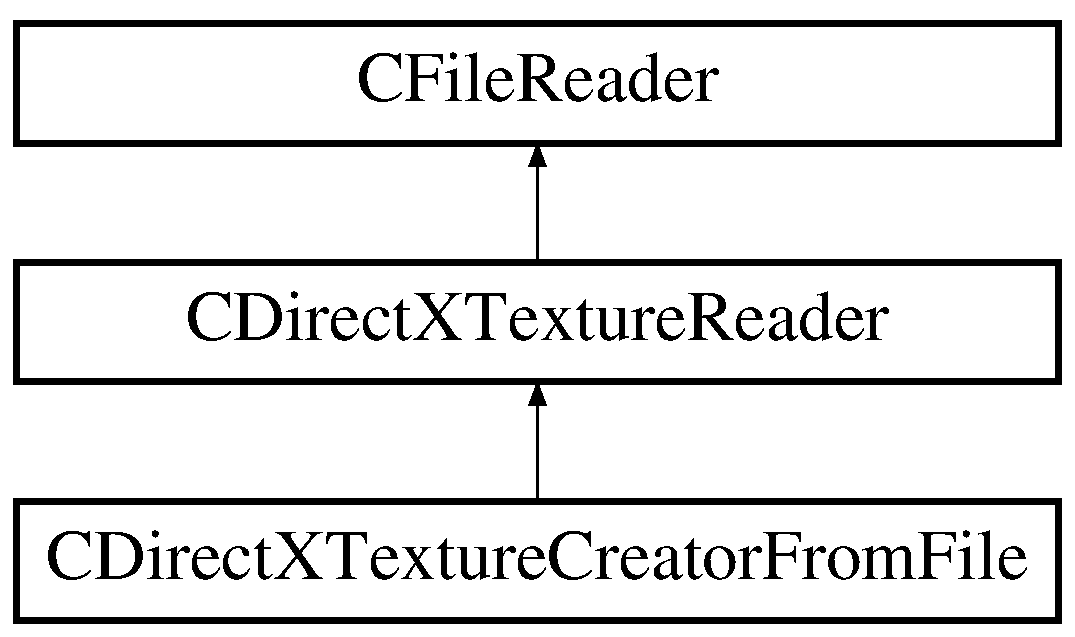
\includegraphics[height=3.000000cm]{class_c_direct_x_texture_creator_from_file}
\end{center}
\end{figure}
\subsection*{公開メンバ関数}
\begin{DoxyCompactItemize}
\item 
\hyperlink{class_c_direct_x_texture_creator_from_file_abc0c74b93240a98b4b12a59bbf343aee}{C\+Direct\+X\+Texture\+Creator\+From\+File} (\hyperlink{class_c_direct_x_texture}{C\+Direct\+X\+Texture} $\ast$\+\_\+pc\+Texture, const T\+Char $\ast$\+\_\+ps\+File\+Name, bool \+\_\+b\+Is\+Suicide)
\begin{DoxyCompactList}\small\item\em コンストラクタ。 \end{DoxyCompactList}\item 
virtual \hyperlink{class_c_direct_x_texture_creator_from_file_af8fccf4bb049bcbe98cd8af63e5bc6dd}{$\sim$\+C\+Direct\+X\+Texture\+Creator\+From\+File} ()
\begin{DoxyCompactList}\small\item\em デストラクタ。 \end{DoxyCompactList}\item 
virtual void \hyperlink{class_c_direct_x_texture_creator_from_file_a5358c62c1a9b7154b17e64d480fa140c}{Read\+End\+Process} (const void $\ast$\+\_\+p\+Data, U\+Size \+\_\+u\+Size) override
\begin{DoxyCompactList}\small\item\em 読み込み完了時の処理。 \end{DoxyCompactList}\item 
virtual void \hyperlink{class_c_direct_x_texture_creator_from_file_aff2a72e9d40761f7654e3b37d6c0b0dd}{Read\+End\+Process\+Sync} () override
\begin{DoxyCompactList}\small\item\em 読み込み完了時の処理(メインスレッドと同期)。 \end{DoxyCompactList}\end{DoxyCompactItemize}
\subsection*{非公開変数類}
\begin{DoxyCompactItemize}
\item 
\hyperlink{class_c_direct_x_texture}{C\+Direct\+X\+Texture} $\ast$ \hyperlink{class_c_direct_x_texture_creator_from_file_a81e5071041c6ebec32e1aeadc1bdcdbe}{m\+\_\+pc\+Texture}
\item 
bool \hyperlink{class_c_direct_x_texture_creator_from_file_ac362400f47c6bd70ddf171af97eea74b}{m\+\_\+b\+Is\+Suicide}
\end{DoxyCompactItemize}


\subsection{構築子と解体子}
\hypertarget{class_c_direct_x_texture_creator_from_file_abc0c74b93240a98b4b12a59bbf343aee}{}\index{C\+Direct\+X\+Texture\+Creator\+From\+File@{C\+Direct\+X\+Texture\+Creator\+From\+File}!C\+Direct\+X\+Texture\+Creator\+From\+File@{C\+Direct\+X\+Texture\+Creator\+From\+File}}
\index{C\+Direct\+X\+Texture\+Creator\+From\+File@{C\+Direct\+X\+Texture\+Creator\+From\+File}!C\+Direct\+X\+Texture\+Creator\+From\+File@{C\+Direct\+X\+Texture\+Creator\+From\+File}}
\subsubsection[{C\+Direct\+X\+Texture\+Creator\+From\+File(\+C\+Direct\+X\+Texture $\ast$\+\_\+pc\+Texture, const T\+Char $\ast$\+\_\+ps\+File\+Name, bool \+\_\+b\+Is\+Suicide)}]{\setlength{\rightskip}{0pt plus 5cm}C\+Direct\+X\+Texture\+Creator\+From\+File\+::\+C\+Direct\+X\+Texture\+Creator\+From\+File (
\begin{DoxyParamCaption}
\item[{{\bf C\+Direct\+X\+Texture} $\ast$}]{\+\_\+pc\+Texture, }
\item[{const T\+Char $\ast$}]{\+\_\+ps\+File\+Name, }
\item[{bool}]{\+\_\+b\+Is\+Suicide}
\end{DoxyParamCaption}
)}\label{class_c_direct_x_texture_creator_from_file_abc0c74b93240a98b4b12a59bbf343aee}


コンストラクタ。 


\begin{DoxyParams}[1]{引数}
\mbox{\tt in}  & {\em \+\_\+pc\+Texture} & \+: テクスチャ作成先。 \\
\hline
\mbox{\tt in}  & {\em \+\_\+ps\+File\+Name} & \+: 画像ファイル名。 \\
\hline
\mbox{\tt in}  & {\em \+\_\+b\+Is\+Suicide} & \+: 作成後自殺するかどうか。 \\
\hline
\end{DoxyParams}
\hypertarget{class_c_direct_x_texture_creator_from_file_af8fccf4bb049bcbe98cd8af63e5bc6dd}{}\index{C\+Direct\+X\+Texture\+Creator\+From\+File@{C\+Direct\+X\+Texture\+Creator\+From\+File}!````~C\+Direct\+X\+Texture\+Creator\+From\+File@{$\sim$\+C\+Direct\+X\+Texture\+Creator\+From\+File}}
\index{````~C\+Direct\+X\+Texture\+Creator\+From\+File@{$\sim$\+C\+Direct\+X\+Texture\+Creator\+From\+File}!C\+Direct\+X\+Texture\+Creator\+From\+File@{C\+Direct\+X\+Texture\+Creator\+From\+File}}
\subsubsection[{$\sim$\+C\+Direct\+X\+Texture\+Creator\+From\+File()}]{\setlength{\rightskip}{0pt plus 5cm}virtual C\+Direct\+X\+Texture\+Creator\+From\+File\+::$\sim$\+C\+Direct\+X\+Texture\+Creator\+From\+File (
\begin{DoxyParamCaption}
{}
\end{DoxyParamCaption}
)\hspace{0.3cm}{\ttfamily [inline]}, {\ttfamily [virtual]}}\label{class_c_direct_x_texture_creator_from_file_af8fccf4bb049bcbe98cd8af63e5bc6dd}


デストラクタ。 



\subsection{関数詳解}
\hypertarget{class_c_direct_x_texture_creator_from_file_a5358c62c1a9b7154b17e64d480fa140c}{}\index{C\+Direct\+X\+Texture\+Creator\+From\+File@{C\+Direct\+X\+Texture\+Creator\+From\+File}!Read\+End\+Process@{Read\+End\+Process}}
\index{Read\+End\+Process@{Read\+End\+Process}!C\+Direct\+X\+Texture\+Creator\+From\+File@{C\+Direct\+X\+Texture\+Creator\+From\+File}}
\subsubsection[{Read\+End\+Process(const void $\ast$\+\_\+p\+Data, U\+Size \+\_\+u\+Size) override}]{\setlength{\rightskip}{0pt plus 5cm}void C\+Direct\+X\+Texture\+Creator\+From\+File\+::\+Read\+End\+Process (
\begin{DoxyParamCaption}
\item[{const void $\ast$}]{\+\_\+p\+Data, }
\item[{U\+Size}]{\+\_\+u\+Size}
\end{DoxyParamCaption}
)\hspace{0.3cm}{\ttfamily [override]}, {\ttfamily [virtual]}}\label{class_c_direct_x_texture_creator_from_file_a5358c62c1a9b7154b17e64d480fa140c}


読み込み完了時の処理。 


\begin{DoxyParams}[1]{引数}
\mbox{\tt in}  & {\em \+\_\+p\+Data} & \+: 読み込んだデータ。 \\
\hline
\mbox{\tt in}  & {\em \+\_\+u\+Size} & \+: 読み込んだデータのサイズ。 \\
\hline
\end{DoxyParams}


\hyperlink{class_c_direct_x_texture_reader_abae2b7a2cf1957d8f0d117851bab35d5}{C\+Direct\+X\+Texture\+Reader}を再実装しています。

\hypertarget{class_c_direct_x_texture_creator_from_file_aff2a72e9d40761f7654e3b37d6c0b0dd}{}\index{C\+Direct\+X\+Texture\+Creator\+From\+File@{C\+Direct\+X\+Texture\+Creator\+From\+File}!Read\+End\+Process\+Sync@{Read\+End\+Process\+Sync}}
\index{Read\+End\+Process\+Sync@{Read\+End\+Process\+Sync}!C\+Direct\+X\+Texture\+Creator\+From\+File@{C\+Direct\+X\+Texture\+Creator\+From\+File}}
\subsubsection[{Read\+End\+Process\+Sync() override}]{\setlength{\rightskip}{0pt plus 5cm}void C\+Direct\+X\+Texture\+Creator\+From\+File\+::\+Read\+End\+Process\+Sync (
\begin{DoxyParamCaption}
{}
\end{DoxyParamCaption}
)\hspace{0.3cm}{\ttfamily [override]}, {\ttfamily [virtual]}}\label{class_c_direct_x_texture_creator_from_file_aff2a72e9d40761f7654e3b37d6c0b0dd}


読み込み完了時の処理(メインスレッドと同期)。 

読み込み完了時の処理(メインスレッドと同期。) 

\hyperlink{class_c_file_reader_ad95360f0d328f570fbc5faf3739732e1}{C\+File\+Reader}を再実装しています。



\subsection{メンバ詳解}
\hypertarget{class_c_direct_x_texture_creator_from_file_ac362400f47c6bd70ddf171af97eea74b}{}\index{C\+Direct\+X\+Texture\+Creator\+From\+File@{C\+Direct\+X\+Texture\+Creator\+From\+File}!m\+\_\+b\+Is\+Suicide@{m\+\_\+b\+Is\+Suicide}}
\index{m\+\_\+b\+Is\+Suicide@{m\+\_\+b\+Is\+Suicide}!C\+Direct\+X\+Texture\+Creator\+From\+File@{C\+Direct\+X\+Texture\+Creator\+From\+File}}
\subsubsection[{m\+\_\+b\+Is\+Suicide}]{\setlength{\rightskip}{0pt plus 5cm}bool C\+Direct\+X\+Texture\+Creator\+From\+File\+::m\+\_\+b\+Is\+Suicide\hspace{0.3cm}{\ttfamily [private]}}\label{class_c_direct_x_texture_creator_from_file_ac362400f47c6bd70ddf171af97eea74b}
\hypertarget{class_c_direct_x_texture_creator_from_file_a81e5071041c6ebec32e1aeadc1bdcdbe}{}\index{C\+Direct\+X\+Texture\+Creator\+From\+File@{C\+Direct\+X\+Texture\+Creator\+From\+File}!m\+\_\+pc\+Texture@{m\+\_\+pc\+Texture}}
\index{m\+\_\+pc\+Texture@{m\+\_\+pc\+Texture}!C\+Direct\+X\+Texture\+Creator\+From\+File@{C\+Direct\+X\+Texture\+Creator\+From\+File}}
\subsubsection[{m\+\_\+pc\+Texture}]{\setlength{\rightskip}{0pt plus 5cm}{\bf C\+Direct\+X\+Texture}$\ast$ C\+Direct\+X\+Texture\+Creator\+From\+File\+::m\+\_\+pc\+Texture\hspace{0.3cm}{\ttfamily [private]}}\label{class_c_direct_x_texture_creator_from_file_a81e5071041c6ebec32e1aeadc1bdcdbe}


このクラス詳解は次のファイルから抽出されました\+:\begin{DoxyCompactItemize}
\item 
D\+:/\+Project/\+Game/\+Lib/\+Direct\+X/\hyperlink{_direct_x_texture_8h}{Direct\+X\+Texture.\+h}\item 
D\+:/\+Project/\+Game/\+Lib/\+Direct\+X/\hyperlink{_direct_x_texture_8cpp}{Direct\+X\+Texture.\+cpp}\end{DoxyCompactItemize}

\hypertarget{class_c_direct_x_texture_reader}{}\section{C\+Direct\+X\+Texture\+Reader クラス}
\label{class_c_direct_x_texture_reader}\index{C\+Direct\+X\+Texture\+Reader@{C\+Direct\+X\+Texture\+Reader}}


{\ttfamily \#include $<$Direct\+X\+Texture.\+h$>$}

C\+Direct\+X\+Texture\+Reader の継承関係図\begin{figure}[H]
\begin{center}
\leavevmode
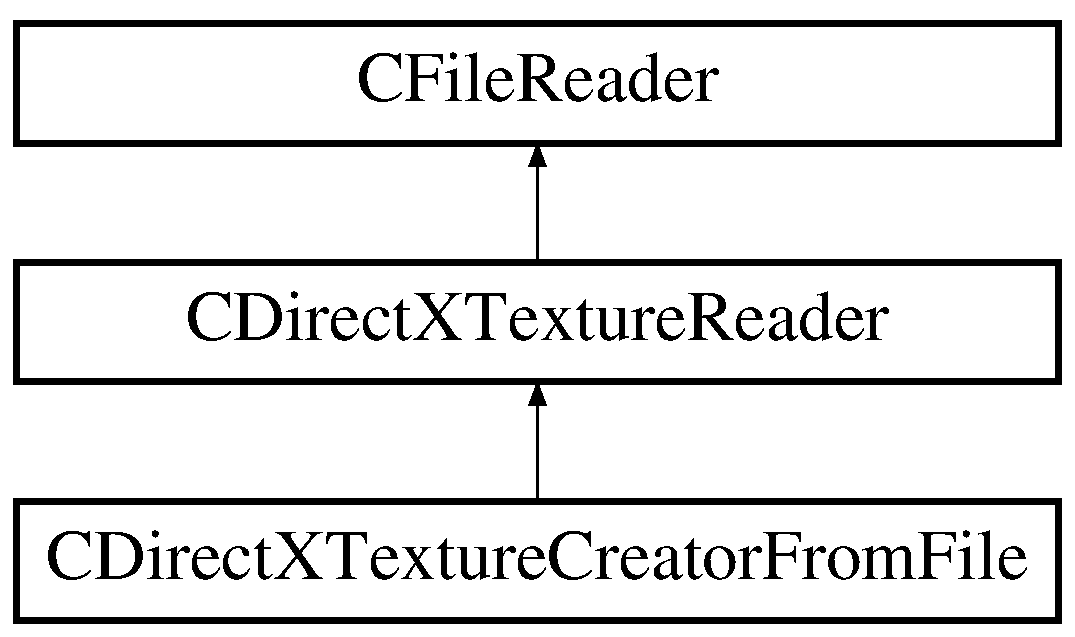
\includegraphics[height=3.000000cm]{class_c_direct_x_texture_reader}
\end{center}
\end{figure}
\subsection*{公開メンバ関数}
\begin{DoxyCompactItemize}
\item 
\hyperlink{class_c_direct_x_texture_reader_a8067f8058a6d70ea0a9ff46aee2ae643}{C\+Direct\+X\+Texture\+Reader} (const T\+Char $\ast$\+\_\+ps\+File\+Name)
\begin{DoxyCompactList}\small\item\em コンストラクタ。 \end{DoxyCompactList}\item 
\hyperlink{class_c_direct_x_texture_reader_af93e4ced10f50fd4070f826f33730f9a}{C\+Direct\+X\+Texture\+Reader} (const T\+Char $\ast$\+\_\+ps\+File\+Name, \hyperlink{namespacen_lib_1_1n_direct_x_a47fcba27656dfc022d6e7ca2a505da65}{n\+Lib\+::n\+Direct\+X\+::\+En\+Texture\+Format} \+\_\+e\+Format)
\item 
virtual \hyperlink{class_c_direct_x_texture_reader_a19885f989b8efc0ae652a27ddfe655e5}{$\sim$\+C\+Direct\+X\+Texture\+Reader} ()
\begin{DoxyCompactList}\small\item\em デストラクタ。 \end{DoxyCompactList}\item 
virtual void \hyperlink{class_c_direct_x_texture_reader_abae2b7a2cf1957d8f0d117851bab35d5}{Read\+End\+Process} (const void $\ast$\+\_\+p\+Data, U\+Size \+\_\+u\+Size) override
\begin{DoxyCompactList}\small\item\em 読み込み完了時の処理。 \end{DoxyCompactList}\item 
const Direct\+X\+::\+Scratch\+Image \& \hyperlink{class_c_direct_x_texture_reader_af12294b81ba5ca060ac58d0b53dfb6e6}{Get\+Image} () const 
\begin{DoxyCompactList}\small\item\em 画像データを取得。 \end{DoxyCompactList}\item 
const Direct\+X\+::\+Tex\+Metadata \& \hyperlink{class_c_direct_x_texture_reader_aaa6dc8a5b66797b9661fc2f13ef642cb}{Get\+Metadata} () const 
\begin{DoxyCompactList}\small\item\em メタデータを取得。 \end{DoxyCompactList}\end{DoxyCompactItemize}
\subsection*{非公開変数類}
\begin{DoxyCompactItemize}
\item 
\hyperlink{namespacen_lib_1_1n_direct_x_a47fcba27656dfc022d6e7ca2a505da65}{n\+Lib\+::n\+Direct\+X\+::\+En\+Texture\+Format} \hyperlink{class_c_direct_x_texture_reader_ac09d73093277f3f444eee39b827fe92c}{m\+\_\+e\+Format}
\item 
Direct\+X\+::\+Scratch\+Image \hyperlink{class_c_direct_x_texture_reader_a3e34a721e8e70a5bf417199c7a5f568b}{m\+\_\+st\+Image}
\item 
Direct\+X\+::\+Tex\+Metadata \hyperlink{class_c_direct_x_texture_reader_a2588eec0104869cb09dd43d9ab2ac024}{m\+\_\+st\+Meta\+Data}
\end{DoxyCompactItemize}


\subsection{構築子と解体子}
\hypertarget{class_c_direct_x_texture_reader_a8067f8058a6d70ea0a9ff46aee2ae643}{}\index{C\+Direct\+X\+Texture\+Reader@{C\+Direct\+X\+Texture\+Reader}!C\+Direct\+X\+Texture\+Reader@{C\+Direct\+X\+Texture\+Reader}}
\index{C\+Direct\+X\+Texture\+Reader@{C\+Direct\+X\+Texture\+Reader}!C\+Direct\+X\+Texture\+Reader@{C\+Direct\+X\+Texture\+Reader}}
\subsubsection[{C\+Direct\+X\+Texture\+Reader(const T\+Char $\ast$\+\_\+ps\+File\+Name)}]{\setlength{\rightskip}{0pt plus 5cm}C\+Direct\+X\+Texture\+Reader\+::\+C\+Direct\+X\+Texture\+Reader (
\begin{DoxyParamCaption}
\item[{const T\+Char $\ast$}]{\+\_\+ps\+File\+Name}
\end{DoxyParamCaption}
)}\label{class_c_direct_x_texture_reader_a8067f8058a6d70ea0a9ff46aee2ae643}


コンストラクタ。 


\begin{DoxyParams}[1]{引数}
\mbox{\tt in}  & {\em \+\_\+ps\+File\+Name} & \+: 読み込むファイル名。 \\
\hline
\end{DoxyParams}
\hypertarget{class_c_direct_x_texture_reader_af93e4ced10f50fd4070f826f33730f9a}{}\index{C\+Direct\+X\+Texture\+Reader@{C\+Direct\+X\+Texture\+Reader}!C\+Direct\+X\+Texture\+Reader@{C\+Direct\+X\+Texture\+Reader}}
\index{C\+Direct\+X\+Texture\+Reader@{C\+Direct\+X\+Texture\+Reader}!C\+Direct\+X\+Texture\+Reader@{C\+Direct\+X\+Texture\+Reader}}
\subsubsection[{C\+Direct\+X\+Texture\+Reader(const T\+Char $\ast$\+\_\+ps\+File\+Name, n\+Lib\+::n\+Direct\+X\+::\+En\+Texture\+Format \+\_\+e\+Format)}]{\setlength{\rightskip}{0pt plus 5cm}C\+Direct\+X\+Texture\+Reader\+::\+C\+Direct\+X\+Texture\+Reader (
\begin{DoxyParamCaption}
\item[{const T\+Char $\ast$}]{\+\_\+ps\+File\+Name, }
\item[{{\bf n\+Lib\+::n\+Direct\+X\+::\+En\+Texture\+Format}}]{\+\_\+e\+Format}
\end{DoxyParamCaption}
)}\label{class_c_direct_x_texture_reader_af93e4ced10f50fd4070f826f33730f9a}
\hypertarget{class_c_direct_x_texture_reader_a19885f989b8efc0ae652a27ddfe655e5}{}\index{C\+Direct\+X\+Texture\+Reader@{C\+Direct\+X\+Texture\+Reader}!````~C\+Direct\+X\+Texture\+Reader@{$\sim$\+C\+Direct\+X\+Texture\+Reader}}
\index{````~C\+Direct\+X\+Texture\+Reader@{$\sim$\+C\+Direct\+X\+Texture\+Reader}!C\+Direct\+X\+Texture\+Reader@{C\+Direct\+X\+Texture\+Reader}}
\subsubsection[{$\sim$\+C\+Direct\+X\+Texture\+Reader()}]{\setlength{\rightskip}{0pt plus 5cm}virtual C\+Direct\+X\+Texture\+Reader\+::$\sim$\+C\+Direct\+X\+Texture\+Reader (
\begin{DoxyParamCaption}
{}
\end{DoxyParamCaption}
)\hspace{0.3cm}{\ttfamily [inline]}, {\ttfamily [virtual]}}\label{class_c_direct_x_texture_reader_a19885f989b8efc0ae652a27ddfe655e5}


デストラクタ。 



\subsection{関数詳解}
\hypertarget{class_c_direct_x_texture_reader_af12294b81ba5ca060ac58d0b53dfb6e6}{}\index{C\+Direct\+X\+Texture\+Reader@{C\+Direct\+X\+Texture\+Reader}!Get\+Image@{Get\+Image}}
\index{Get\+Image@{Get\+Image}!C\+Direct\+X\+Texture\+Reader@{C\+Direct\+X\+Texture\+Reader}}
\subsubsection[{Get\+Image() const }]{\setlength{\rightskip}{0pt plus 5cm}const Direct\+X\+::\+Scratch\+Image\& C\+Direct\+X\+Texture\+Reader\+::\+Get\+Image (
\begin{DoxyParamCaption}
{}
\end{DoxyParamCaption}
) const\hspace{0.3cm}{\ttfamily [inline]}}\label{class_c_direct_x_texture_reader_af12294b81ba5ca060ac58d0b53dfb6e6}


画像データを取得。 

\hypertarget{class_c_direct_x_texture_reader_aaa6dc8a5b66797b9661fc2f13ef642cb}{}\index{C\+Direct\+X\+Texture\+Reader@{C\+Direct\+X\+Texture\+Reader}!Get\+Metadata@{Get\+Metadata}}
\index{Get\+Metadata@{Get\+Metadata}!C\+Direct\+X\+Texture\+Reader@{C\+Direct\+X\+Texture\+Reader}}
\subsubsection[{Get\+Metadata() const }]{\setlength{\rightskip}{0pt plus 5cm}const Direct\+X\+::\+Tex\+Metadata\& C\+Direct\+X\+Texture\+Reader\+::\+Get\+Metadata (
\begin{DoxyParamCaption}
{}
\end{DoxyParamCaption}
) const\hspace{0.3cm}{\ttfamily [inline]}}\label{class_c_direct_x_texture_reader_aaa6dc8a5b66797b9661fc2f13ef642cb}


メタデータを取得。 

\hypertarget{class_c_direct_x_texture_reader_abae2b7a2cf1957d8f0d117851bab35d5}{}\index{C\+Direct\+X\+Texture\+Reader@{C\+Direct\+X\+Texture\+Reader}!Read\+End\+Process@{Read\+End\+Process}}
\index{Read\+End\+Process@{Read\+End\+Process}!C\+Direct\+X\+Texture\+Reader@{C\+Direct\+X\+Texture\+Reader}}
\subsubsection[{Read\+End\+Process(const void $\ast$\+\_\+p\+Data, U\+Size \+\_\+u\+Size) override}]{\setlength{\rightskip}{0pt plus 5cm}void C\+Direct\+X\+Texture\+Reader\+::\+Read\+End\+Process (
\begin{DoxyParamCaption}
\item[{const void $\ast$}]{\+\_\+p\+Data, }
\item[{U\+Size}]{\+\_\+u\+Size}
\end{DoxyParamCaption}
)\hspace{0.3cm}{\ttfamily [override]}, {\ttfamily [virtual]}}\label{class_c_direct_x_texture_reader_abae2b7a2cf1957d8f0d117851bab35d5}


読み込み完了時の処理。 


\begin{DoxyParams}[1]{引数}
\mbox{\tt in}  & {\em \+\_\+p\+Data} & \+: 読み込んだデータ。 \\
\hline
\mbox{\tt in}  & {\em \+\_\+u\+Size} & \+: 読み込んだデータのサイズ。 \\
\hline
\end{DoxyParams}


\hyperlink{class_c_file_reader_a5a18550133826ac43096629f6eaa8c42}{C\+File\+Reader}を再実装しています。



\hyperlink{class_c_direct_x_texture_creator_from_file_a5358c62c1a9b7154b17e64d480fa140c}{C\+Direct\+X\+Texture\+Creator\+From\+File}で再実装されています。



\subsection{メンバ詳解}
\hypertarget{class_c_direct_x_texture_reader_ac09d73093277f3f444eee39b827fe92c}{}\index{C\+Direct\+X\+Texture\+Reader@{C\+Direct\+X\+Texture\+Reader}!m\+\_\+e\+Format@{m\+\_\+e\+Format}}
\index{m\+\_\+e\+Format@{m\+\_\+e\+Format}!C\+Direct\+X\+Texture\+Reader@{C\+Direct\+X\+Texture\+Reader}}
\subsubsection[{m\+\_\+e\+Format}]{\setlength{\rightskip}{0pt plus 5cm}{\bf n\+Lib\+::n\+Direct\+X\+::\+En\+Texture\+Format} C\+Direct\+X\+Texture\+Reader\+::m\+\_\+e\+Format\hspace{0.3cm}{\ttfamily [private]}}\label{class_c_direct_x_texture_reader_ac09d73093277f3f444eee39b827fe92c}
\hypertarget{class_c_direct_x_texture_reader_a3e34a721e8e70a5bf417199c7a5f568b}{}\index{C\+Direct\+X\+Texture\+Reader@{C\+Direct\+X\+Texture\+Reader}!m\+\_\+st\+Image@{m\+\_\+st\+Image}}
\index{m\+\_\+st\+Image@{m\+\_\+st\+Image}!C\+Direct\+X\+Texture\+Reader@{C\+Direct\+X\+Texture\+Reader}}
\subsubsection[{m\+\_\+st\+Image}]{\setlength{\rightskip}{0pt plus 5cm}Direct\+X\+::\+Scratch\+Image C\+Direct\+X\+Texture\+Reader\+::m\+\_\+st\+Image\hspace{0.3cm}{\ttfamily [private]}}\label{class_c_direct_x_texture_reader_a3e34a721e8e70a5bf417199c7a5f568b}
\hypertarget{class_c_direct_x_texture_reader_a2588eec0104869cb09dd43d9ab2ac024}{}\index{C\+Direct\+X\+Texture\+Reader@{C\+Direct\+X\+Texture\+Reader}!m\+\_\+st\+Meta\+Data@{m\+\_\+st\+Meta\+Data}}
\index{m\+\_\+st\+Meta\+Data@{m\+\_\+st\+Meta\+Data}!C\+Direct\+X\+Texture\+Reader@{C\+Direct\+X\+Texture\+Reader}}
\subsubsection[{m\+\_\+st\+Meta\+Data}]{\setlength{\rightskip}{0pt plus 5cm}Direct\+X\+::\+Tex\+Metadata C\+Direct\+X\+Texture\+Reader\+::m\+\_\+st\+Meta\+Data\hspace{0.3cm}{\ttfamily [private]}}\label{class_c_direct_x_texture_reader_a2588eec0104869cb09dd43d9ab2ac024}


このクラス詳解は次のファイルから抽出されました\+:\begin{DoxyCompactItemize}
\item 
D\+:/\+Project/\+Game/\+Lib/\+Direct\+X/\hyperlink{_direct_x_texture_8h}{Direct\+X\+Texture.\+h}\item 
D\+:/\+Project/\+Game/\+Lib/\+Direct\+X/\hyperlink{_direct_x_texture_8cpp}{Direct\+X\+Texture.\+cpp}\end{DoxyCompactItemize}

\hypertarget{class_c_draw}{}\section{C\+Draw クラス}
\label{class_c_draw}\index{C\+Draw@{C\+Draw}}


{\ttfamily \#include $<$Draw.\+h$>$}

\subsection*{公開メンバ関数}
\begin{DoxyCompactItemize}
\item 
virtual void \hyperlink{class_c_draw_ad47eba2cc4c42c22054840fd01188113}{Draw} (\hyperlink{class_i_render_context}{I\+Render\+Context} $\ast$\+\_\+pc\+Render\+Context)
\begin{DoxyCompactList}\small\item\em 描画処理。 \end{DoxyCompactList}\item 
void \hyperlink{class_c_draw_a488b15c0d5ab2804ef17041c660c0ee4}{Set\+Active\+Draw} (bool \+\_\+b\+Active)
\begin{DoxyCompactList}\small\item\em アクティブフラグの設定。 \end{DoxyCompactList}\item 
bool \hyperlink{class_c_draw_a03be67979fa5b246e836254ad1e4bacc}{Is\+Active\+Draw} () const 
\begin{DoxyCompactList}\small\item\em アクティブフラグの取得。 \end{DoxyCompactList}\item 
U32 \hyperlink{class_c_draw_af3f2ed5336c01a4c58cab3441859cbba}{Get\+Draw\+Lv} () const 
\begin{DoxyCompactList}\small\item\em 描画レベルの取得。 \end{DoxyCompactList}\end{DoxyCompactItemize}
\subsection*{限定公開メンバ関数}
\begin{DoxyCompactItemize}
\item 
\hyperlink{class_c_draw_afb80462217185decc321ec9c087b5dbf}{C\+Draw} (U32 \+\_\+u\+Draw\+Lv)
\begin{DoxyCompactList}\small\item\em コンストラクタ。 \end{DoxyCompactList}\item 
virtual \hyperlink{class_c_draw_a4eac2e28e3797347574590ab302a1807}{$\sim$\+C\+Draw} ()
\begin{DoxyCompactList}\small\item\em デストラクタ。 \end{DoxyCompactList}\end{DoxyCompactItemize}
\subsection*{非公開変数類}
\begin{DoxyCompactItemize}
\item 
U32 \hyperlink{class_c_draw_ac89d726cd678e124e8acc20730e66107}{m\+\_\+u\+Draw\+Lv}
\item 
bool \hyperlink{class_c_draw_a62288bb9680c3584db7295cbd1c45f5d}{m\+\_\+b\+Active}
\end{DoxyCompactItemize}


\subsection{構築子と解体子}
\hypertarget{class_c_draw_afb80462217185decc321ec9c087b5dbf}{}\index{C\+Draw@{C\+Draw}!C\+Draw@{C\+Draw}}
\index{C\+Draw@{C\+Draw}!C\+Draw@{C\+Draw}}
\subsubsection[{C\+Draw(\+U32 \+\_\+u\+Draw\+Lv)}]{\setlength{\rightskip}{0pt plus 5cm}C\+Draw\+::\+C\+Draw (
\begin{DoxyParamCaption}
\item[{U32}]{\+\_\+u\+Draw\+Lv}
\end{DoxyParamCaption}
)\hspace{0.3cm}{\ttfamily [protected]}}\label{class_c_draw_afb80462217185decc321ec9c087b5dbf}


コンストラクタ。 


\begin{DoxyParams}{引数}
{\em \+\_\+u\+Draw\+Lv} & \+: 描画レベル。 \\
\hline
\end{DoxyParams}
\hypertarget{class_c_draw_a4eac2e28e3797347574590ab302a1807}{}\index{C\+Draw@{C\+Draw}!````~C\+Draw@{$\sim$\+C\+Draw}}
\index{````~C\+Draw@{$\sim$\+C\+Draw}!C\+Draw@{C\+Draw}}
\subsubsection[{$\sim$\+C\+Draw()}]{\setlength{\rightskip}{0pt plus 5cm}C\+Draw\+::$\sim$\+C\+Draw (
\begin{DoxyParamCaption}
{}
\end{DoxyParamCaption}
)\hspace{0.3cm}{\ttfamily [protected]}, {\ttfamily [virtual]}}\label{class_c_draw_a4eac2e28e3797347574590ab302a1807}


デストラクタ。 



\subsection{関数詳解}
\hypertarget{class_c_draw_ad47eba2cc4c42c22054840fd01188113}{}\index{C\+Draw@{C\+Draw}!Draw@{Draw}}
\index{Draw@{Draw}!C\+Draw@{C\+Draw}}
\subsubsection[{Draw(\+I\+Render\+Context $\ast$\+\_\+pc\+Render\+Context)}]{\setlength{\rightskip}{0pt plus 5cm}virtual void C\+Draw\+::\+Draw (
\begin{DoxyParamCaption}
\item[{{\bf I\+Render\+Context} $\ast$}]{\+\_\+pc\+Render\+Context}
\end{DoxyParamCaption}
)\hspace{0.3cm}{\ttfamily [inline]}, {\ttfamily [virtual]}}\label{class_c_draw_ad47eba2cc4c42c22054840fd01188113}


描画処理。 

\hypertarget{class_c_draw_af3f2ed5336c01a4c58cab3441859cbba}{}\index{C\+Draw@{C\+Draw}!Get\+Draw\+Lv@{Get\+Draw\+Lv}}
\index{Get\+Draw\+Lv@{Get\+Draw\+Lv}!C\+Draw@{C\+Draw}}
\subsubsection[{Get\+Draw\+Lv() const }]{\setlength{\rightskip}{0pt plus 5cm}U32 C\+Draw\+::\+Get\+Draw\+Lv (
\begin{DoxyParamCaption}
{}
\end{DoxyParamCaption}
) const\hspace{0.3cm}{\ttfamily [inline]}}\label{class_c_draw_af3f2ed5336c01a4c58cab3441859cbba}


描画レベルの取得。 

\hypertarget{class_c_draw_a03be67979fa5b246e836254ad1e4bacc}{}\index{C\+Draw@{C\+Draw}!Is\+Active\+Draw@{Is\+Active\+Draw}}
\index{Is\+Active\+Draw@{Is\+Active\+Draw}!C\+Draw@{C\+Draw}}
\subsubsection[{Is\+Active\+Draw() const }]{\setlength{\rightskip}{0pt plus 5cm}bool C\+Draw\+::\+Is\+Active\+Draw (
\begin{DoxyParamCaption}
{}
\end{DoxyParamCaption}
) const\hspace{0.3cm}{\ttfamily [inline]}}\label{class_c_draw_a03be67979fa5b246e836254ad1e4bacc}


アクティブフラグの取得。 

\hypertarget{class_c_draw_a488b15c0d5ab2804ef17041c660c0ee4}{}\index{C\+Draw@{C\+Draw}!Set\+Active\+Draw@{Set\+Active\+Draw}}
\index{Set\+Active\+Draw@{Set\+Active\+Draw}!C\+Draw@{C\+Draw}}
\subsubsection[{Set\+Active\+Draw(bool \+\_\+b\+Active)}]{\setlength{\rightskip}{0pt plus 5cm}void C\+Draw\+::\+Set\+Active\+Draw (
\begin{DoxyParamCaption}
\item[{bool}]{\+\_\+b\+Active}
\end{DoxyParamCaption}
)\hspace{0.3cm}{\ttfamily [inline]}}\label{class_c_draw_a488b15c0d5ab2804ef17041c660c0ee4}


アクティブフラグの設定。 



\subsection{メンバ詳解}
\hypertarget{class_c_draw_a62288bb9680c3584db7295cbd1c45f5d}{}\index{C\+Draw@{C\+Draw}!m\+\_\+b\+Active@{m\+\_\+b\+Active}}
\index{m\+\_\+b\+Active@{m\+\_\+b\+Active}!C\+Draw@{C\+Draw}}
\subsubsection[{m\+\_\+b\+Active}]{\setlength{\rightskip}{0pt plus 5cm}bool C\+Draw\+::m\+\_\+b\+Active\hspace{0.3cm}{\ttfamily [private]}}\label{class_c_draw_a62288bb9680c3584db7295cbd1c45f5d}
\hypertarget{class_c_draw_ac89d726cd678e124e8acc20730e66107}{}\index{C\+Draw@{C\+Draw}!m\+\_\+u\+Draw\+Lv@{m\+\_\+u\+Draw\+Lv}}
\index{m\+\_\+u\+Draw\+Lv@{m\+\_\+u\+Draw\+Lv}!C\+Draw@{C\+Draw}}
\subsubsection[{m\+\_\+u\+Draw\+Lv}]{\setlength{\rightskip}{0pt plus 5cm}U32 C\+Draw\+::m\+\_\+u\+Draw\+Lv\hspace{0.3cm}{\ttfamily [private]}}\label{class_c_draw_ac89d726cd678e124e8acc20730e66107}


このクラス詳解は次のファイルから抽出されました\+:\begin{DoxyCompactItemize}
\item 
D\+:/\+Project/\+Game/\+Lib/\+Object/\hyperlink{_draw_8h}{Draw.\+h}\item 
D\+:/\+Project/\+Game/\+Lib/\+Object/\hyperlink{_draw_8cpp}{Draw.\+cpp}\end{DoxyCompactItemize}

\hypertarget{class_c_draw_list}{}\section{C\+Draw\+List クラス}
\label{class_c_draw_list}\index{C\+Draw\+List@{C\+Draw\+List}}


{\ttfamily \#include $<$Draw\+List.\+h$>$}

C\+Draw\+List の継承関係図\begin{figure}[H]
\begin{center}
\leavevmode
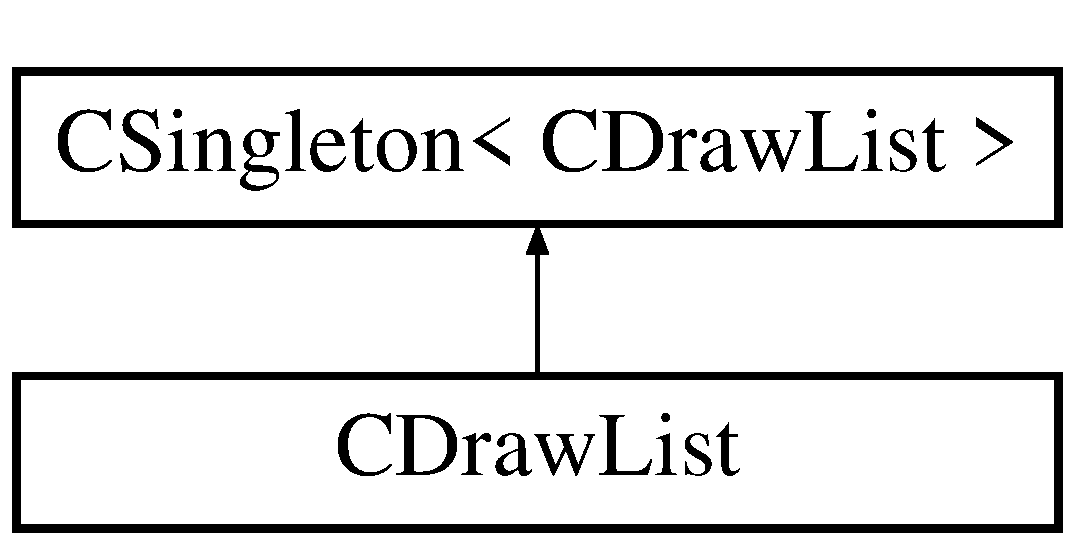
\includegraphics[height=2.000000cm]{class_c_draw_list}
\end{center}
\end{figure}
\subsection*{クラス}
\begin{DoxyCompactItemize}
\item 
struct \hyperlink{struct_c_draw_list_1_1_st_init_param}{St\+Init\+Param}
\begin{DoxyCompactList}\small\item\em 初期化用構造体。 \end{DoxyCompactList}\end{DoxyCompactItemize}
\subsection*{公開メンバ関数}
\begin{DoxyCompactItemize}
\item 
virtual \hyperlink{class_c_draw_list_a6331b9e423dac5cc0d2405d5088535c0}{$\sim$\+C\+Draw\+List} ()
\begin{DoxyCompactList}\small\item\em デストラクタ。 \end{DoxyCompactList}\item 
void \hyperlink{class_c_draw_list_a56e19a77d7ed33e6009df5aea2f1848c}{Init} (const \hyperlink{struct_c_draw_list_1_1_st_init_param}{St\+Init\+Param} \&\+\_\+rst\+Param)
\begin{DoxyCompactList}\small\item\em 初期化。 \end{DoxyCompactList}\item 
void \hyperlink{class_c_draw_list_a6ecfdbccf9d8e817fc8f304e76f3b4a4}{Register} (\hyperlink{class_c_draw}{C\+Draw} $\ast$\+\_\+p\+Object)
\begin{DoxyCompactList}\small\item\em 登録処理。 \end{DoxyCompactList}\item 
void \hyperlink{class_c_draw_list_a6cbdc83efffd556cac5b7d7f03910936}{Un\+Register} (\hyperlink{class_c_draw}{C\+Draw} $\ast$\+\_\+p\+Object)
\begin{DoxyCompactList}\small\item\em 解除処理。 \end{DoxyCompactList}\item 
void \hyperlink{class_c_draw_list_a9cb8d446fb669b158e662fd6f460af9a}{All\+Draw} (\hyperlink{class_i_render_context}{I\+Render\+Context} $\ast$\+\_\+pc\+Render\+Context)
\begin{DoxyCompactList}\small\item\em 全てのオブジェクトの描画処理を実行。 \end{DoxyCompactList}\end{DoxyCompactItemize}
\subsection*{限定公開変数類}
\begin{DoxyCompactItemize}
\item 
\hyperlink{struct_c_draw_list_1_1_st_init_param}{St\+Init\+Param} \hyperlink{class_c_draw_list_aa1852cdf435d6e0d1b0057bfa29115ef}{m\+\_\+st\+Param}
\item 
\hyperlink{class_c_object_list}{C\+Object\+List}$<$ \hyperlink{class_c_draw}{C\+Draw} $>$ $\ast$ \hyperlink{class_c_draw_list_a9657465a848a483be27ca0fbb41af73a}{m\+\_\+pc\+Draw\+List}
\end{DoxyCompactItemize}
\subsection*{非公開メンバ関数}
\begin{DoxyCompactItemize}
\item 
\hyperlink{class_c_draw_list_a6aa66199590e8434c4f405c2d2105f54}{C\+Draw\+List} ()
\begin{DoxyCompactList}\small\item\em コンストラクタ。 \end{DoxyCompactList}\end{DoxyCompactItemize}
\subsection*{非公開変数類}
\begin{DoxyCompactItemize}
\item 
friend \hyperlink{class_c_draw_list_ace89c5af0071b6f1a4798baf330cd9a0}{C\+Singleton$<$ C\+Draw\+List $>$}
\end{DoxyCompactItemize}
\subsection*{その他の継承メンバ}


\subsection{構築子と解体子}
\hypertarget{class_c_draw_list_a6aa66199590e8434c4f405c2d2105f54}{}\index{C\+Draw\+List@{C\+Draw\+List}!C\+Draw\+List@{C\+Draw\+List}}
\index{C\+Draw\+List@{C\+Draw\+List}!C\+Draw\+List@{C\+Draw\+List}}
\subsubsection[{C\+Draw\+List()}]{\setlength{\rightskip}{0pt plus 5cm}C\+Draw\+List\+::\+C\+Draw\+List (
\begin{DoxyParamCaption}
{}
\end{DoxyParamCaption}
)\hspace{0.3cm}{\ttfamily [private]}}\label{class_c_draw_list_a6aa66199590e8434c4f405c2d2105f54}


コンストラクタ。 

\hypertarget{class_c_draw_list_a6331b9e423dac5cc0d2405d5088535c0}{}\index{C\+Draw\+List@{C\+Draw\+List}!````~C\+Draw\+List@{$\sim$\+C\+Draw\+List}}
\index{````~C\+Draw\+List@{$\sim$\+C\+Draw\+List}!C\+Draw\+List@{C\+Draw\+List}}
\subsubsection[{$\sim$\+C\+Draw\+List()}]{\setlength{\rightskip}{0pt plus 5cm}C\+Draw\+List\+::$\sim$\+C\+Draw\+List (
\begin{DoxyParamCaption}
{}
\end{DoxyParamCaption}
)\hspace{0.3cm}{\ttfamily [virtual]}}\label{class_c_draw_list_a6331b9e423dac5cc0d2405d5088535c0}


デストラクタ。 



\subsection{関数詳解}
\hypertarget{class_c_draw_list_a9cb8d446fb669b158e662fd6f460af9a}{}\index{C\+Draw\+List@{C\+Draw\+List}!All\+Draw@{All\+Draw}}
\index{All\+Draw@{All\+Draw}!C\+Draw\+List@{C\+Draw\+List}}
\subsubsection[{All\+Draw(\+I\+Render\+Context $\ast$\+\_\+pc\+Render\+Context)}]{\setlength{\rightskip}{0pt plus 5cm}void C\+Draw\+List\+::\+All\+Draw (
\begin{DoxyParamCaption}
\item[{{\bf I\+Render\+Context} $\ast$}]{\+\_\+pc\+Render\+Context}
\end{DoxyParamCaption}
)}\label{class_c_draw_list_a9cb8d446fb669b158e662fd6f460af9a}


全てのオブジェクトの描画処理を実行。 


\begin{DoxyParams}[1]{引数}
\mbox{\tt in}  & {\em \+\_\+pc\+Render\+Context} & \+: 描画コンテキスト。 \\
\hline
\end{DoxyParams}
\hypertarget{class_c_draw_list_a56e19a77d7ed33e6009df5aea2f1848c}{}\index{C\+Draw\+List@{C\+Draw\+List}!Init@{Init}}
\index{Init@{Init}!C\+Draw\+List@{C\+Draw\+List}}
\subsubsection[{Init(const St\+Init\+Param \&\+\_\+rst\+Param)}]{\setlength{\rightskip}{0pt plus 5cm}void C\+Draw\+List\+::\+Init (
\begin{DoxyParamCaption}
\item[{const {\bf St\+Init\+Param} \&}]{\+\_\+rst\+Param}
\end{DoxyParamCaption}
)}\label{class_c_draw_list_a56e19a77d7ed33e6009df5aea2f1848c}


初期化。 


\begin{DoxyParams}[1]{引数}
\mbox{\tt in}  & {\em \+\_\+rst\+Param} & \+: 初期化用パラメータ。 \\
\hline
\end{DoxyParams}
\hypertarget{class_c_draw_list_a6ecfdbccf9d8e817fc8f304e76f3b4a4}{}\index{C\+Draw\+List@{C\+Draw\+List}!Register@{Register}}
\index{Register@{Register}!C\+Draw\+List@{C\+Draw\+List}}
\subsubsection[{Register(\+C\+Draw $\ast$\+\_\+p\+Object)}]{\setlength{\rightskip}{0pt plus 5cm}void C\+Draw\+List\+::\+Register (
\begin{DoxyParamCaption}
\item[{{\bf C\+Draw} $\ast$}]{\+\_\+p\+Object}
\end{DoxyParamCaption}
)}\label{class_c_draw_list_a6ecfdbccf9d8e817fc8f304e76f3b4a4}


登録処理。 


\begin{DoxyParams}[1]{引数}
\mbox{\tt in}  & {\em \+\_\+p\+Object} & \+: 登録するオブジェクト。 \\
\hline
\end{DoxyParams}
\hypertarget{class_c_draw_list_a6cbdc83efffd556cac5b7d7f03910936}{}\index{C\+Draw\+List@{C\+Draw\+List}!Un\+Register@{Un\+Register}}
\index{Un\+Register@{Un\+Register}!C\+Draw\+List@{C\+Draw\+List}}
\subsubsection[{Un\+Register(\+C\+Draw $\ast$\+\_\+p\+Object)}]{\setlength{\rightskip}{0pt plus 5cm}void C\+Draw\+List\+::\+Un\+Register (
\begin{DoxyParamCaption}
\item[{{\bf C\+Draw} $\ast$}]{\+\_\+p\+Object}
\end{DoxyParamCaption}
)}\label{class_c_draw_list_a6cbdc83efffd556cac5b7d7f03910936}


解除処理。 


\begin{DoxyParams}[1]{引数}
\mbox{\tt in}  & {\em \+\_\+p\+Object} & \+: 解除するオブジェクト。 \\
\hline
\end{DoxyParams}


\subsection{メンバ詳解}
\hypertarget{class_c_draw_list_ace89c5af0071b6f1a4798baf330cd9a0}{}\index{C\+Draw\+List@{C\+Draw\+List}!C\+Singleton$<$ C\+Draw\+List $>$@{C\+Singleton$<$ C\+Draw\+List $>$}}
\index{C\+Singleton$<$ C\+Draw\+List $>$@{C\+Singleton$<$ C\+Draw\+List $>$}!C\+Draw\+List@{C\+Draw\+List}}
\subsubsection[{C\+Singleton$<$ C\+Draw\+List $>$}]{\setlength{\rightskip}{0pt plus 5cm}friend {\bf C\+Draw\+List\+::\+C\+Singleton}$<$ {\bf C\+Draw\+List} $>$\hspace{0.3cm}{\ttfamily [private]}}\label{class_c_draw_list_ace89c5af0071b6f1a4798baf330cd9a0}
\hypertarget{class_c_draw_list_a9657465a848a483be27ca0fbb41af73a}{}\index{C\+Draw\+List@{C\+Draw\+List}!m\+\_\+pc\+Draw\+List@{m\+\_\+pc\+Draw\+List}}
\index{m\+\_\+pc\+Draw\+List@{m\+\_\+pc\+Draw\+List}!C\+Draw\+List@{C\+Draw\+List}}
\subsubsection[{m\+\_\+pc\+Draw\+List}]{\setlength{\rightskip}{0pt plus 5cm}{\bf C\+Object\+List}$<$ {\bf C\+Draw} $>$$\ast$ C\+Draw\+List\+::m\+\_\+pc\+Draw\+List\hspace{0.3cm}{\ttfamily [protected]}}\label{class_c_draw_list_a9657465a848a483be27ca0fbb41af73a}
\hypertarget{class_c_draw_list_aa1852cdf435d6e0d1b0057bfa29115ef}{}\index{C\+Draw\+List@{C\+Draw\+List}!m\+\_\+st\+Param@{m\+\_\+st\+Param}}
\index{m\+\_\+st\+Param@{m\+\_\+st\+Param}!C\+Draw\+List@{C\+Draw\+List}}
\subsubsection[{m\+\_\+st\+Param}]{\setlength{\rightskip}{0pt plus 5cm}{\bf St\+Init\+Param} C\+Draw\+List\+::m\+\_\+st\+Param\hspace{0.3cm}{\ttfamily [protected]}}\label{class_c_draw_list_aa1852cdf435d6e0d1b0057bfa29115ef}


このクラス詳解は次のファイルから抽出されました\+:\begin{DoxyCompactItemize}
\item 
D\+:/\+Project/\+Game/\+Lib/\+Object/\hyperlink{_draw_list_8h}{Draw\+List.\+h}\item 
D\+:/\+Project/\+Game/\+Lib/\+Object/\hyperlink{_draw_list_8cpp}{Draw\+List.\+cpp}\end{DoxyCompactItemize}

\hypertarget{class_c_draw_lv}{}\section{C\+Draw\+Lv クラス}
\label{class_c_draw_lv}\index{C\+Draw\+Lv@{C\+Draw\+Lv}}


{\ttfamily \#include $<$Draw\+Lv.\+h$>$}

\subsection*{公開型}
\begin{DoxyCompactItemize}
\item 
enum \hyperlink{class_c_draw_lv_a45316dff9df4c5a2991f1eb0ca758ae9}{En\+Draw\+Lv} \+: U32 \{ \hyperlink{class_c_draw_lv_a45316dff9df4c5a2991f1eb0ca758ae9a0557fa923dcee4d0f86b1409f5c2167f}{En\+Draw\+Lv\+::\+Back} = 0, 
\hyperlink{class_c_draw_lv_a45316dff9df4c5a2991f1eb0ca758ae9ab1ca34f82e83c52b010f86955f264e05}{En\+Draw\+Lv\+::\+Middle}, 
\hyperlink{class_c_draw_lv_a45316dff9df4c5a2991f1eb0ca758ae9a5835bab1ade0060909e31a06af2e2cde}{En\+Draw\+Lv\+::\+Front}, 
\hyperlink{class_c_draw_lv_a45316dff9df4c5a2991f1eb0ca758ae9a6a061313d22e51e0f25b7cd4dc065233}{En\+Draw\+Lv\+::\+Max}
 \}
\end{DoxyCompactItemize}
\subsection*{静的公開メンバ関数}
\begin{DoxyCompactItemize}
\item 
static U32 \hyperlink{class_c_draw_lv_ab612b9c3b7b7b5c50267d3020231d874}{Back} ()
\item 
static U32 \hyperlink{class_c_draw_lv_a505ac52f3df1c06de45de912601c3b2a}{Middle} ()
\item 
static U32 \hyperlink{class_c_draw_lv_abe93b0ac399cf46bb9f142eca58f1764}{Front} ()
\item 
static U32 \hyperlink{class_c_draw_lv_affca7747ae2c87b67f06223d89b3eb1f}{Max} ()
\end{DoxyCompactItemize}


\subsection{列挙型メンバ詳解}
\hypertarget{class_c_draw_lv_a45316dff9df4c5a2991f1eb0ca758ae9}{}\index{C\+Draw\+Lv@{C\+Draw\+Lv}!En\+Draw\+Lv@{En\+Draw\+Lv}}
\index{En\+Draw\+Lv@{En\+Draw\+Lv}!C\+Draw\+Lv@{C\+Draw\+Lv}}
\subsubsection[{En\+Draw\+Lv}]{\setlength{\rightskip}{0pt plus 5cm}enum {\bf C\+Draw\+Lv\+::\+En\+Draw\+Lv} \+: U32\hspace{0.3cm}{\ttfamily [strong]}}\label{class_c_draw_lv_a45316dff9df4c5a2991f1eb0ca758ae9}
\begin{Desc}
\item[列挙値]\par
\begin{description}
\index{Back@{Back}!C\+Draw\+Lv@{C\+Draw\+Lv}}\index{C\+Draw\+Lv@{C\+Draw\+Lv}!Back@{Back}}\item[{\em 
\hypertarget{class_c_draw_lv_a45316dff9df4c5a2991f1eb0ca758ae9a0557fa923dcee4d0f86b1409f5c2167f}{}Back\label{class_c_draw_lv_a45316dff9df4c5a2991f1eb0ca758ae9a0557fa923dcee4d0f86b1409f5c2167f}
}]\index{Middle@{Middle}!C\+Draw\+Lv@{C\+Draw\+Lv}}\index{C\+Draw\+Lv@{C\+Draw\+Lv}!Middle@{Middle}}\item[{\em 
\hypertarget{class_c_draw_lv_a45316dff9df4c5a2991f1eb0ca758ae9ab1ca34f82e83c52b010f86955f264e05}{}Middle\label{class_c_draw_lv_a45316dff9df4c5a2991f1eb0ca758ae9ab1ca34f82e83c52b010f86955f264e05}
}]\index{Front@{Front}!C\+Draw\+Lv@{C\+Draw\+Lv}}\index{C\+Draw\+Lv@{C\+Draw\+Lv}!Front@{Front}}\item[{\em 
\hypertarget{class_c_draw_lv_a45316dff9df4c5a2991f1eb0ca758ae9a5835bab1ade0060909e31a06af2e2cde}{}Front\label{class_c_draw_lv_a45316dff9df4c5a2991f1eb0ca758ae9a5835bab1ade0060909e31a06af2e2cde}
}]\index{Max@{Max}!C\+Draw\+Lv@{C\+Draw\+Lv}}\index{C\+Draw\+Lv@{C\+Draw\+Lv}!Max@{Max}}\item[{\em 
\hypertarget{class_c_draw_lv_a45316dff9df4c5a2991f1eb0ca758ae9a6a061313d22e51e0f25b7cd4dc065233}{}Max\label{class_c_draw_lv_a45316dff9df4c5a2991f1eb0ca758ae9a6a061313d22e51e0f25b7cd4dc065233}
}]\end{description}
\end{Desc}


\subsection{関数詳解}
\hypertarget{class_c_draw_lv_ab612b9c3b7b7b5c50267d3020231d874}{}\index{C\+Draw\+Lv@{C\+Draw\+Lv}!Back@{Back}}
\index{Back@{Back}!C\+Draw\+Lv@{C\+Draw\+Lv}}
\subsubsection[{Back()}]{\setlength{\rightskip}{0pt plus 5cm}static U32 C\+Draw\+Lv\+::\+Back (
\begin{DoxyParamCaption}
{}
\end{DoxyParamCaption}
)\hspace{0.3cm}{\ttfamily [inline]}, {\ttfamily [static]}}\label{class_c_draw_lv_ab612b9c3b7b7b5c50267d3020231d874}
\hypertarget{class_c_draw_lv_abe93b0ac399cf46bb9f142eca58f1764}{}\index{C\+Draw\+Lv@{C\+Draw\+Lv}!Front@{Front}}
\index{Front@{Front}!C\+Draw\+Lv@{C\+Draw\+Lv}}
\subsubsection[{Front()}]{\setlength{\rightskip}{0pt plus 5cm}static U32 C\+Draw\+Lv\+::\+Front (
\begin{DoxyParamCaption}
{}
\end{DoxyParamCaption}
)\hspace{0.3cm}{\ttfamily [inline]}, {\ttfamily [static]}}\label{class_c_draw_lv_abe93b0ac399cf46bb9f142eca58f1764}
\hypertarget{class_c_draw_lv_affca7747ae2c87b67f06223d89b3eb1f}{}\index{C\+Draw\+Lv@{C\+Draw\+Lv}!Max@{Max}}
\index{Max@{Max}!C\+Draw\+Lv@{C\+Draw\+Lv}}
\subsubsection[{Max()}]{\setlength{\rightskip}{0pt plus 5cm}static U32 C\+Draw\+Lv\+::\+Max (
\begin{DoxyParamCaption}
{}
\end{DoxyParamCaption}
)\hspace{0.3cm}{\ttfamily [inline]}, {\ttfamily [static]}}\label{class_c_draw_lv_affca7747ae2c87b67f06223d89b3eb1f}
\hypertarget{class_c_draw_lv_a505ac52f3df1c06de45de912601c3b2a}{}\index{C\+Draw\+Lv@{C\+Draw\+Lv}!Middle@{Middle}}
\index{Middle@{Middle}!C\+Draw\+Lv@{C\+Draw\+Lv}}
\subsubsection[{Middle()}]{\setlength{\rightskip}{0pt plus 5cm}static U32 C\+Draw\+Lv\+::\+Middle (
\begin{DoxyParamCaption}
{}
\end{DoxyParamCaption}
)\hspace{0.3cm}{\ttfamily [inline]}, {\ttfamily [static]}}\label{class_c_draw_lv_a505ac52f3df1c06de45de912601c3b2a}


このクラス詳解は次のファイルから抽出されました\+:\begin{DoxyCompactItemize}
\item 
D\+:/\+Project/\+Game/\hyperlink{_draw_lv_8h}{Draw\+Lv.\+h}\end{DoxyCompactItemize}

\hypertarget{class_c_file_reader}{}\section{C\+File\+Reader クラス}
\label{class_c_file_reader}\index{C\+File\+Reader@{C\+File\+Reader}}


{\ttfamily \#include $<$File\+Reader.\+h$>$}

C\+File\+Reader の継承関係図\begin{figure}[H]
\begin{center}
\leavevmode
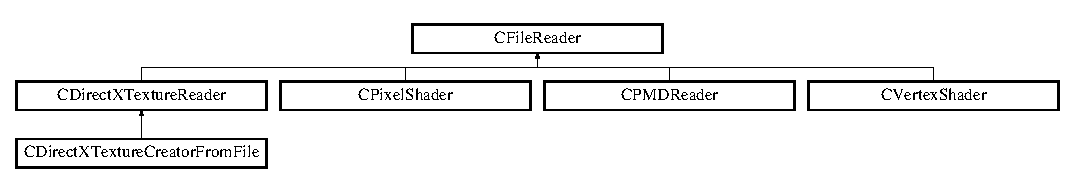
\includegraphics[height=2.028986cm]{class_c_file_reader}
\end{center}
\end{figure}
\subsection*{公開メンバ関数}
\begin{DoxyCompactItemize}
\item 
\hyperlink{class_c_file_reader_ac1c1601d5d3fea0418cc561a979fa5b4}{C\+File\+Reader} (const T\+Char $\ast$\+\_\+ps\+File\+Name)
\begin{DoxyCompactList}\small\item\em コンストラクタ。 \end{DoxyCompactList}\item 
virtual \hyperlink{class_c_file_reader_a4d1f50d0e41e3de38890100df04325b2}{$\sim$\+C\+File\+Reader} ()
\begin{DoxyCompactList}\small\item\em デストラクタ。 \end{DoxyCompactList}\item 
virtual void \hyperlink{class_c_file_reader_a5a18550133826ac43096629f6eaa8c42}{Read\+End\+Process} (const void $\ast$\+\_\+p\+Data, U\+Size \+\_\+u\+Size)
\begin{DoxyCompactList}\small\item\em 読み込み完了時の処理。 \end{DoxyCompactList}\item 
virtual void \hyperlink{class_c_file_reader_ad95360f0d328f570fbc5faf3739732e1}{Read\+End\+Process\+Sync} ()
\begin{DoxyCompactList}\small\item\em 読み込み完了時の処理(メインスレッドと同期)。 \end{DoxyCompactList}\item 
const T\+Char $\ast$ \hyperlink{class_c_file_reader_ae59f3337c42c1ca9e26a46336f52bd96}{Get\+File\+Name} () const 
\begin{DoxyCompactList}\small\item\em 読み込むファイル名を取得。 \end{DoxyCompactList}\item 
bool \hyperlink{class_c_file_reader_ae354b54f0ebdbbf5bf59c773004cef6b}{Is\+Read\+End} () const 
\begin{DoxyCompactList}\small\item\em 読み込みが完了したか。 \end{DoxyCompactList}\item 
void \hyperlink{class_c_file_reader_a0f04fd0be744cccb3a057e6cfd2cecd1}{Set\+Read\+End} (bool \+\_\+b\+End)
\begin{DoxyCompactList}\small\item\em 読み込みが完了したか設定。 \end{DoxyCompactList}\end{DoxyCompactItemize}
\subsection*{非公開変数類}
\begin{DoxyCompactItemize}
\item 
\hyperlink{_string_8h_a65b002fe7fe31f6e84dbb7e46907e031}{C\+T\+String} \hyperlink{class_c_file_reader_a336f2d904f2b316d584b7fba8f996d69}{m\+\_\+c\+File\+Name}
\item 
bool \hyperlink{class_c_file_reader_a1eeeadefb7a22567093fca3f1efbc1d7}{m\+\_\+b\+Is\+Read\+End}
\end{DoxyCompactItemize}


\subsection{構築子と解体子}
\hypertarget{class_c_file_reader_ac1c1601d5d3fea0418cc561a979fa5b4}{}\index{C\+File\+Reader@{C\+File\+Reader}!C\+File\+Reader@{C\+File\+Reader}}
\index{C\+File\+Reader@{C\+File\+Reader}!C\+File\+Reader@{C\+File\+Reader}}
\subsubsection[{C\+File\+Reader(const T\+Char $\ast$\+\_\+ps\+File\+Name)}]{\setlength{\rightskip}{0pt plus 5cm}C\+File\+Reader\+::\+C\+File\+Reader (
\begin{DoxyParamCaption}
\item[{const T\+Char $\ast$}]{\+\_\+ps\+File\+Name}
\end{DoxyParamCaption}
)}\label{class_c_file_reader_ac1c1601d5d3fea0418cc561a979fa5b4}


コンストラクタ。 


\begin{DoxyParams}[1]{引数}
\mbox{\tt in}  & {\em \+\_\+ps\+File\+Name} & \+: 読み込むファイルネーム。 \\
\hline
\end{DoxyParams}
\hypertarget{class_c_file_reader_a4d1f50d0e41e3de38890100df04325b2}{}\index{C\+File\+Reader@{C\+File\+Reader}!````~C\+File\+Reader@{$\sim$\+C\+File\+Reader}}
\index{````~C\+File\+Reader@{$\sim$\+C\+File\+Reader}!C\+File\+Reader@{C\+File\+Reader}}
\subsubsection[{$\sim$\+C\+File\+Reader()}]{\setlength{\rightskip}{0pt plus 5cm}virtual C\+File\+Reader\+::$\sim$\+C\+File\+Reader (
\begin{DoxyParamCaption}
{}
\end{DoxyParamCaption}
)\hspace{0.3cm}{\ttfamily [inline]}, {\ttfamily [virtual]}}\label{class_c_file_reader_a4d1f50d0e41e3de38890100df04325b2}


デストラクタ。 



\subsection{関数詳解}
\hypertarget{class_c_file_reader_ae59f3337c42c1ca9e26a46336f52bd96}{}\index{C\+File\+Reader@{C\+File\+Reader}!Get\+File\+Name@{Get\+File\+Name}}
\index{Get\+File\+Name@{Get\+File\+Name}!C\+File\+Reader@{C\+File\+Reader}}
\subsubsection[{Get\+File\+Name() const }]{\setlength{\rightskip}{0pt plus 5cm}const T\+Char$\ast$ C\+File\+Reader\+::\+Get\+File\+Name (
\begin{DoxyParamCaption}
{}
\end{DoxyParamCaption}
) const\hspace{0.3cm}{\ttfamily [inline]}}\label{class_c_file_reader_ae59f3337c42c1ca9e26a46336f52bd96}


読み込むファイル名を取得。 

\hypertarget{class_c_file_reader_ae354b54f0ebdbbf5bf59c773004cef6b}{}\index{C\+File\+Reader@{C\+File\+Reader}!Is\+Read\+End@{Is\+Read\+End}}
\index{Is\+Read\+End@{Is\+Read\+End}!C\+File\+Reader@{C\+File\+Reader}}
\subsubsection[{Is\+Read\+End() const }]{\setlength{\rightskip}{0pt plus 5cm}bool C\+File\+Reader\+::\+Is\+Read\+End (
\begin{DoxyParamCaption}
{}
\end{DoxyParamCaption}
) const\hspace{0.3cm}{\ttfamily [inline]}}\label{class_c_file_reader_ae354b54f0ebdbbf5bf59c773004cef6b}


読み込みが完了したか。 

\hypertarget{class_c_file_reader_a5a18550133826ac43096629f6eaa8c42}{}\index{C\+File\+Reader@{C\+File\+Reader}!Read\+End\+Process@{Read\+End\+Process}}
\index{Read\+End\+Process@{Read\+End\+Process}!C\+File\+Reader@{C\+File\+Reader}}
\subsubsection[{Read\+End\+Process(const void $\ast$\+\_\+p\+Data, U\+Size \+\_\+u\+Size)}]{\setlength{\rightskip}{0pt plus 5cm}virtual void C\+File\+Reader\+::\+Read\+End\+Process (
\begin{DoxyParamCaption}
\item[{const void $\ast$}]{\+\_\+p\+Data, }
\item[{U\+Size}]{\+\_\+u\+Size}
\end{DoxyParamCaption}
)\hspace{0.3cm}{\ttfamily [inline]}, {\ttfamily [virtual]}}\label{class_c_file_reader_a5a18550133826ac43096629f6eaa8c42}


読み込み完了時の処理。 



\hyperlink{class_c_direct_x_texture_creator_from_file_a5358c62c1a9b7154b17e64d480fa140c}{C\+Direct\+X\+Texture\+Creator\+From\+File}, \hyperlink{class_c_direct_x_texture_reader_abae2b7a2cf1957d8f0d117851bab35d5}{C\+Direct\+X\+Texture\+Reader}, \hyperlink{class_c_pixel_shader_a5a70cfcd3b998c6f55f4c95f351e940e}{C\+Pixel\+Shader}, \hyperlink{class_c_vertex_shader_a6e640bce4b58ca267c39b9287a973c3b}{C\+Vertex\+Shader}, \hyperlink{class_c_p_m_d_reader_a326af26b1815aaa4b088b037fb76e05f}{C\+P\+M\+D\+Reader}で再実装されています。

\hypertarget{class_c_file_reader_ad95360f0d328f570fbc5faf3739732e1}{}\index{C\+File\+Reader@{C\+File\+Reader}!Read\+End\+Process\+Sync@{Read\+End\+Process\+Sync}}
\index{Read\+End\+Process\+Sync@{Read\+End\+Process\+Sync}!C\+File\+Reader@{C\+File\+Reader}}
\subsubsection[{Read\+End\+Process\+Sync()}]{\setlength{\rightskip}{0pt plus 5cm}virtual void C\+File\+Reader\+::\+Read\+End\+Process\+Sync (
\begin{DoxyParamCaption}
{}
\end{DoxyParamCaption}
)\hspace{0.3cm}{\ttfamily [inline]}, {\ttfamily [virtual]}}\label{class_c_file_reader_ad95360f0d328f570fbc5faf3739732e1}


読み込み完了時の処理(メインスレッドと同期)。 



\hyperlink{class_c_direct_x_texture_creator_from_file_aff2a72e9d40761f7654e3b37d6c0b0dd}{C\+Direct\+X\+Texture\+Creator\+From\+File}で再実装されています。

\hypertarget{class_c_file_reader_a0f04fd0be744cccb3a057e6cfd2cecd1}{}\index{C\+File\+Reader@{C\+File\+Reader}!Set\+Read\+End@{Set\+Read\+End}}
\index{Set\+Read\+End@{Set\+Read\+End}!C\+File\+Reader@{C\+File\+Reader}}
\subsubsection[{Set\+Read\+End(bool \+\_\+b\+End)}]{\setlength{\rightskip}{0pt plus 5cm}void C\+File\+Reader\+::\+Set\+Read\+End (
\begin{DoxyParamCaption}
\item[{bool}]{\+\_\+b\+End}
\end{DoxyParamCaption}
)\hspace{0.3cm}{\ttfamily [inline]}}\label{class_c_file_reader_a0f04fd0be744cccb3a057e6cfd2cecd1}


読み込みが完了したか設定。 



\subsection{メンバ詳解}
\hypertarget{class_c_file_reader_a1eeeadefb7a22567093fca3f1efbc1d7}{}\index{C\+File\+Reader@{C\+File\+Reader}!m\+\_\+b\+Is\+Read\+End@{m\+\_\+b\+Is\+Read\+End}}
\index{m\+\_\+b\+Is\+Read\+End@{m\+\_\+b\+Is\+Read\+End}!C\+File\+Reader@{C\+File\+Reader}}
\subsubsection[{m\+\_\+b\+Is\+Read\+End}]{\setlength{\rightskip}{0pt plus 5cm}bool C\+File\+Reader\+::m\+\_\+b\+Is\+Read\+End\hspace{0.3cm}{\ttfamily [private]}}\label{class_c_file_reader_a1eeeadefb7a22567093fca3f1efbc1d7}
\hypertarget{class_c_file_reader_a336f2d904f2b316d584b7fba8f996d69}{}\index{C\+File\+Reader@{C\+File\+Reader}!m\+\_\+c\+File\+Name@{m\+\_\+c\+File\+Name}}
\index{m\+\_\+c\+File\+Name@{m\+\_\+c\+File\+Name}!C\+File\+Reader@{C\+File\+Reader}}
\subsubsection[{m\+\_\+c\+File\+Name}]{\setlength{\rightskip}{0pt plus 5cm}{\bf C\+T\+String} C\+File\+Reader\+::m\+\_\+c\+File\+Name\hspace{0.3cm}{\ttfamily [private]}}\label{class_c_file_reader_a336f2d904f2b316d584b7fba8f996d69}


このクラス詳解は次のファイルから抽出されました\+:\begin{DoxyCompactItemize}
\item 
D\+:/\+Project/\+Game/\+Lib/\+File/\hyperlink{_file_reader_8h}{File\+Reader.\+h}\item 
D\+:/\+Project/\+Game/\+Lib/\+File/\hyperlink{_file_reader_8cpp}{File\+Reader.\+cpp}\end{DoxyCompactItemize}

\hypertarget{class_c_file_read_manager}{}\section{C\+File\+Read\+Manager クラス}
\label{class_c_file_read_manager}\index{C\+File\+Read\+Manager@{C\+File\+Read\+Manager}}


{\ttfamily \#include $<$File\+Read\+Manager.\+h$>$}

C\+File\+Read\+Manager の継承関係図\begin{figure}[H]
\begin{center}
\leavevmode
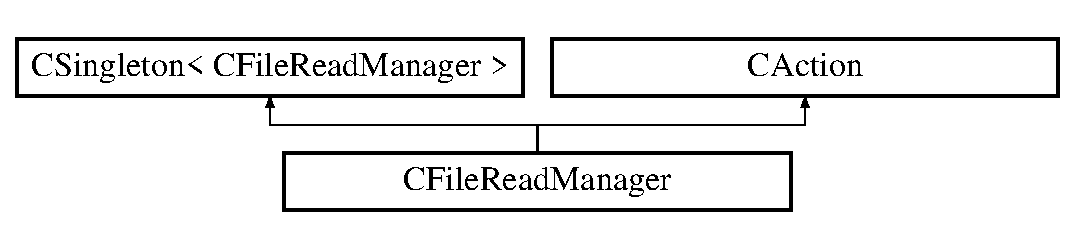
\includegraphics[height=2.000000cm]{class_c_file_read_manager}
\end{center}
\end{figure}
\subsection*{クラス}
\begin{DoxyCompactItemize}
\item 
struct \hyperlink{struct_c_file_read_manager_1_1_st_init_param}{St\+Init\+Param}
\begin{DoxyCompactList}\small\item\em 初期化用パラメータ。 \end{DoxyCompactList}\end{DoxyCompactItemize}
\subsection*{公開メンバ関数}
\begin{DoxyCompactItemize}
\item 
virtual \hyperlink{class_c_file_read_manager_a1ef0e31d0e5d89fe0722f124a312438c}{$\sim$\+C\+File\+Read\+Manager} ()
\begin{DoxyCompactList}\small\item\em デストラクタ。 \end{DoxyCompactList}\item 
void \hyperlink{class_c_file_read_manager_a0bd09488d14efeed36b3445188391d34}{Request} (\hyperlink{class_c_file_reader}{C\+File\+Reader} $\ast$\+\_\+pc\+File\+Reader)
\begin{DoxyCompactList}\small\item\em ファイル読み込みリクエスト。 \end{DoxyCompactList}\item 
virtual void \hyperlink{class_c_file_read_manager_a1c0c420814fed21f257b71740c56a365}{Action} () override
\begin{DoxyCompactList}\small\item\em アクション処理。 \end{DoxyCompactList}\end{DoxyCompactItemize}
\subsection*{静的公開メンバ関数}
\begin{DoxyCompactItemize}
\item 
static void \hyperlink{class_c_file_read_manager_a2be2641a242706bb410e976325a74665}{Create\+Instance} (const \hyperlink{struct_c_file_read_manager_1_1_st_init_param}{St\+Init\+Param} \&\+\_\+rst\+Param)
\begin{DoxyCompactList}\small\item\em インスタンス作成。 \end{DoxyCompactList}\end{DoxyCompactItemize}
\subsection*{非公開メンバ関数}
\begin{DoxyCompactItemize}
\item 
\hyperlink{class_c_file_read_manager_a3eafa43bdf03c4b3560900d952c6eb22}{C\+File\+Read\+Manager} ()
\begin{DoxyCompactList}\small\item\em コンストラクタ。 \end{DoxyCompactList}\item 
\hyperlink{class_c_file_read_manager_a75ad845bcfe35443ef29d2a2cfe843cd}{C\+File\+Read\+Manager} (const \hyperlink{struct_c_file_read_manager_1_1_st_init_param}{St\+Init\+Param} \&\+\_\+rst\+Param)
\end{DoxyCompactItemize}
\subsection*{非公開変数類}
\begin{DoxyCompactItemize}
\item 
friend \hyperlink{class_c_file_read_manager_a7a9788832ab00f7595c2782a849942e9}{C\+Singleton$<$ C\+File\+Read\+Manager $>$}
\item 
\hyperlink{_list_8h_af54c38acd8944230f18792ac38211526}{C\+Vector}$<$ \hyperlink{class_c_job_file_read}{C\+Job\+File\+Read} $\ast$ $>$ \hyperlink{class_c_file_read_manager_a06d2dd73e1e01a66e4072ecfe4507c54}{m\+\_\+c\+Job\+List}
\end{DoxyCompactItemize}
\subsection*{その他の継承メンバ}


\subsection{構築子と解体子}
\hypertarget{class_c_file_read_manager_a3eafa43bdf03c4b3560900d952c6eb22}{}\index{C\+File\+Read\+Manager@{C\+File\+Read\+Manager}!C\+File\+Read\+Manager@{C\+File\+Read\+Manager}}
\index{C\+File\+Read\+Manager@{C\+File\+Read\+Manager}!C\+File\+Read\+Manager@{C\+File\+Read\+Manager}}
\subsubsection[{C\+File\+Read\+Manager()}]{\setlength{\rightskip}{0pt plus 5cm}C\+File\+Read\+Manager\+::\+C\+File\+Read\+Manager (
\begin{DoxyParamCaption}
{}
\end{DoxyParamCaption}
)\hspace{0.3cm}{\ttfamily [private]}}\label{class_c_file_read_manager_a3eafa43bdf03c4b3560900d952c6eb22}


コンストラクタ。 

\hypertarget{class_c_file_read_manager_a75ad845bcfe35443ef29d2a2cfe843cd}{}\index{C\+File\+Read\+Manager@{C\+File\+Read\+Manager}!C\+File\+Read\+Manager@{C\+File\+Read\+Manager}}
\index{C\+File\+Read\+Manager@{C\+File\+Read\+Manager}!C\+File\+Read\+Manager@{C\+File\+Read\+Manager}}
\subsubsection[{C\+File\+Read\+Manager(const St\+Init\+Param \&\+\_\+rst\+Param)}]{\setlength{\rightskip}{0pt plus 5cm}C\+File\+Read\+Manager\+::\+C\+File\+Read\+Manager (
\begin{DoxyParamCaption}
\item[{const {\bf St\+Init\+Param} \&}]{\+\_\+rst\+Param}
\end{DoxyParamCaption}
)\hspace{0.3cm}{\ttfamily [private]}}\label{class_c_file_read_manager_a75ad845bcfe35443ef29d2a2cfe843cd}
\hypertarget{class_c_file_read_manager_a1ef0e31d0e5d89fe0722f124a312438c}{}\index{C\+File\+Read\+Manager@{C\+File\+Read\+Manager}!````~C\+File\+Read\+Manager@{$\sim$\+C\+File\+Read\+Manager}}
\index{````~C\+File\+Read\+Manager@{$\sim$\+C\+File\+Read\+Manager}!C\+File\+Read\+Manager@{C\+File\+Read\+Manager}}
\subsubsection[{$\sim$\+C\+File\+Read\+Manager()}]{\setlength{\rightskip}{0pt plus 5cm}C\+File\+Read\+Manager\+::$\sim$\+C\+File\+Read\+Manager (
\begin{DoxyParamCaption}
{}
\end{DoxyParamCaption}
)\hspace{0.3cm}{\ttfamily [virtual]}}\label{class_c_file_read_manager_a1ef0e31d0e5d89fe0722f124a312438c}


デストラクタ。 



\subsection{関数詳解}
\hypertarget{class_c_file_read_manager_a1c0c420814fed21f257b71740c56a365}{}\index{C\+File\+Read\+Manager@{C\+File\+Read\+Manager}!Action@{Action}}
\index{Action@{Action}!C\+File\+Read\+Manager@{C\+File\+Read\+Manager}}
\subsubsection[{Action() override}]{\setlength{\rightskip}{0pt plus 5cm}void C\+File\+Read\+Manager\+::\+Action (
\begin{DoxyParamCaption}
{}
\end{DoxyParamCaption}
)\hspace{0.3cm}{\ttfamily [override]}, {\ttfamily [virtual]}}\label{class_c_file_read_manager_a1c0c420814fed21f257b71740c56a365}


アクション処理。 



\hyperlink{class_c_action_a3fcc5cc0fde844c5cb6e50f7eec9da3c}{C\+Action}を再実装しています。

\hypertarget{class_c_file_read_manager_a2be2641a242706bb410e976325a74665}{}\index{C\+File\+Read\+Manager@{C\+File\+Read\+Manager}!Create\+Instance@{Create\+Instance}}
\index{Create\+Instance@{Create\+Instance}!C\+File\+Read\+Manager@{C\+File\+Read\+Manager}}
\subsubsection[{Create\+Instance(const St\+Init\+Param \&\+\_\+rst\+Param)}]{\setlength{\rightskip}{0pt plus 5cm}static void C\+File\+Read\+Manager\+::\+Create\+Instance (
\begin{DoxyParamCaption}
\item[{const {\bf St\+Init\+Param} \&}]{\+\_\+rst\+Param}
\end{DoxyParamCaption}
)\hspace{0.3cm}{\ttfamily [inline]}, {\ttfamily [static]}}\label{class_c_file_read_manager_a2be2641a242706bb410e976325a74665}


インスタンス作成。 

\hypertarget{class_c_file_read_manager_a0bd09488d14efeed36b3445188391d34}{}\index{C\+File\+Read\+Manager@{C\+File\+Read\+Manager}!Request@{Request}}
\index{Request@{Request}!C\+File\+Read\+Manager@{C\+File\+Read\+Manager}}
\subsubsection[{Request(\+C\+File\+Reader $\ast$\+\_\+pc\+File\+Reader)}]{\setlength{\rightskip}{0pt plus 5cm}void C\+File\+Read\+Manager\+::\+Request (
\begin{DoxyParamCaption}
\item[{{\bf C\+File\+Reader} $\ast$}]{\+\_\+pc\+File\+Reader}
\end{DoxyParamCaption}
)}\label{class_c_file_read_manager_a0bd09488d14efeed36b3445188391d34}


ファイル読み込みリクエスト。 


\begin{DoxyParams}[1]{引数}
\mbox{\tt in}  & {\em \+\_\+pc\+File\+Reader} & \+: ファイル読み込みクラスへのポインタ。 \\
\hline
\end{DoxyParams}


\subsection{メンバ詳解}
\hypertarget{class_c_file_read_manager_a7a9788832ab00f7595c2782a849942e9}{}\index{C\+File\+Read\+Manager@{C\+File\+Read\+Manager}!C\+Singleton$<$ C\+File\+Read\+Manager $>$@{C\+Singleton$<$ C\+File\+Read\+Manager $>$}}
\index{C\+Singleton$<$ C\+File\+Read\+Manager $>$@{C\+Singleton$<$ C\+File\+Read\+Manager $>$}!C\+File\+Read\+Manager@{C\+File\+Read\+Manager}}
\subsubsection[{C\+Singleton$<$ C\+File\+Read\+Manager $>$}]{\setlength{\rightskip}{0pt plus 5cm}friend {\bf C\+File\+Read\+Manager\+::\+C\+Singleton}$<$ {\bf C\+File\+Read\+Manager} $>$\hspace{0.3cm}{\ttfamily [private]}}\label{class_c_file_read_manager_a7a9788832ab00f7595c2782a849942e9}
\hypertarget{class_c_file_read_manager_a06d2dd73e1e01a66e4072ecfe4507c54}{}\index{C\+File\+Read\+Manager@{C\+File\+Read\+Manager}!m\+\_\+c\+Job\+List@{m\+\_\+c\+Job\+List}}
\index{m\+\_\+c\+Job\+List@{m\+\_\+c\+Job\+List}!C\+File\+Read\+Manager@{C\+File\+Read\+Manager}}
\subsubsection[{m\+\_\+c\+Job\+List}]{\setlength{\rightskip}{0pt plus 5cm}{\bf C\+Vector}$<${\bf C\+Job\+File\+Read}$\ast$$>$ C\+File\+Read\+Manager\+::m\+\_\+c\+Job\+List\hspace{0.3cm}{\ttfamily [private]}}\label{class_c_file_read_manager_a06d2dd73e1e01a66e4072ecfe4507c54}


このクラス詳解は次のファイルから抽出されました\+:\begin{DoxyCompactItemize}
\item 
D\+:/\+Project/\+Game/\+Lib/\+File/\hyperlink{_file_read_manager_8h}{File\+Read\+Manager.\+h}\item 
D\+:/\+Project/\+Game/\+Lib/\+File/\hyperlink{_file_read_manager_8cpp}{File\+Read\+Manager.\+cpp}\end{DoxyCompactItemize}

\hypertarget{class_c_file_read_thread}{}\section{C\+File\+Read\+Thread クラス}
\label{class_c_file_read_thread}\index{C\+File\+Read\+Thread@{C\+File\+Read\+Thread}}


{\ttfamily \#include $<$File\+Read\+Thread.\+h$>$}

C\+File\+Read\+Thread の継承関係図\begin{figure}[H]
\begin{center}
\leavevmode
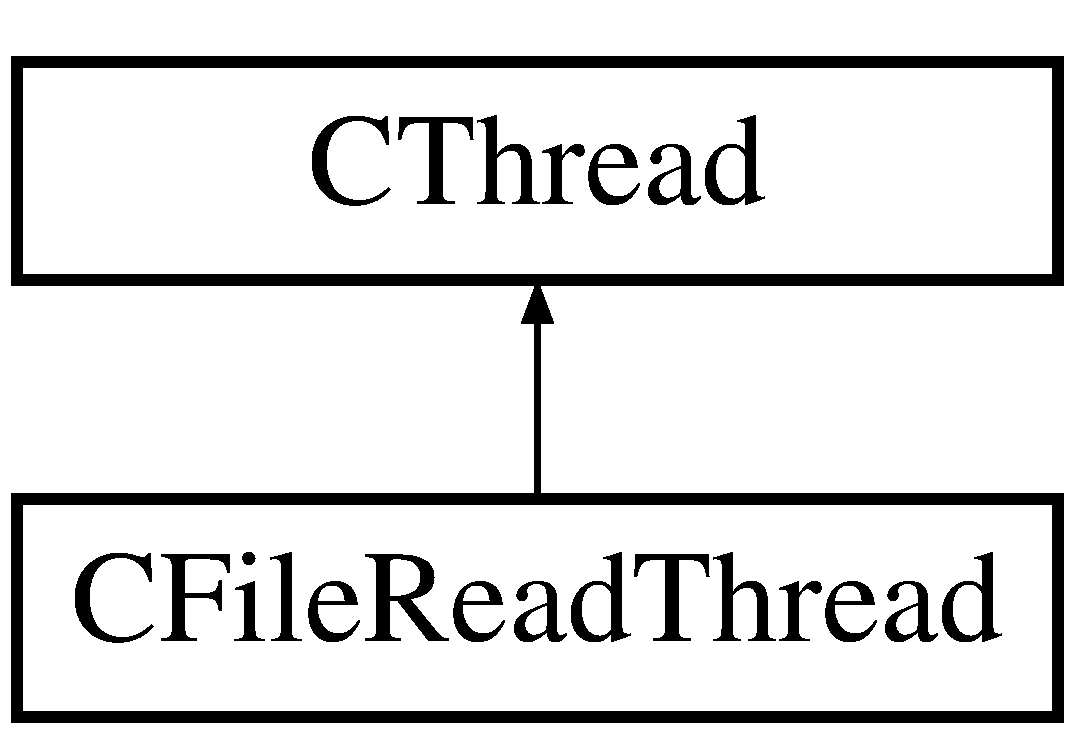
\includegraphics[height=2.000000cm]{class_c_file_read_thread}
\end{center}
\end{figure}
\subsection*{公開メンバ関数}
\begin{DoxyCompactItemize}
\item 
\hyperlink{class_c_file_read_thread_a6be058890450e1457324d738a42324e8}{C\+File\+Read\+Thread} ()
\begin{DoxyCompactList}\small\item\em コンストラクタ。 \end{DoxyCompactList}\item 
virtual \hyperlink{class_c_file_read_thread_a249a969dafa6aa1fb98b87098f3d9f22}{$\sim$\+C\+File\+Read\+Thread} ()
\begin{DoxyCompactList}\small\item\em デストラクタ。 \end{DoxyCompactList}\item 
virtual void \hyperlink{class_c_file_read_thread_a74368d5091a88e1ad149e35a09fba026}{Thread\+Callback} () override
\begin{DoxyCompactList}\small\item\em 開始したスレッドから呼ばれるコールバック関数。 \end{DoxyCompactList}\item 
void \hyperlink{class_c_file_read_thread_a93688d92c0a249522ab133a4de08b727}{Request} (const T\+Char $\ast$\+\_\+ps\+File\+Name)
\begin{DoxyCompactList}\small\item\em ファイル読み込みリクエスト。 \end{DoxyCompactList}\item 
void \hyperlink{class_c_file_read_thread_a36a83980898059b75c22fb0e9fba9b8c}{Request\+End\+Thread} ()
\begin{DoxyCompactList}\small\item\em スレッド終了リクエスト。 \end{DoxyCompactList}\item 
bool \hyperlink{class_c_file_read_thread_a67df23cd8c25bb51a414838353576c6c}{Is\+Read\+End} ()
\begin{DoxyCompactList}\small\item\em 読み込みが終了したか。 \end{DoxyCompactList}\item 
void $\ast$ \hyperlink{class_c_file_read_thread_a13d5df9d60ab84216882cd4791b88f46}{Get\+Data} ()
\begin{DoxyCompactList}\small\item\em 読み込んだデータを取得。 \end{DoxyCompactList}\item 
U\+Size \hyperlink{class_c_file_read_thread_ae89ecd3f84e68aa48eea6f3ed787484c}{Get\+Size} ()
\begin{DoxyCompactList}\small\item\em 読み込んだデータサイズを取得。 \end{DoxyCompactList}\end{DoxyCompactItemize}
\subsection*{非公開変数類}
\begin{DoxyCompactItemize}
\item 
\hyperlink{_string_8h_a65b002fe7fe31f6e84dbb7e46907e031}{C\+T\+String} \hyperlink{class_c_file_read_thread_a6a9ea67314b0dc1e77f3eb0b2ab16cf3}{m\+\_\+c\+File\+Name}
\item 
bool \hyperlink{class_c_file_read_thread_abca3c8548dd1eb8c48d052c20819e928}{m\+\_\+b\+Is\+Request}
\item 
bool \hyperlink{class_c_file_read_thread_acb76507c5a24b0cc3f7ccb1339712419}{m\+\_\+b\+Is\+Read\+End}
\item 
bool \hyperlink{class_c_file_read_thread_a00e36c8dc11b75c8f555afe0a0f84dbf}{m\+\_\+b\+Request\+End}
\item 
void $\ast$ \hyperlink{class_c_file_read_thread_aa185614299cc1f92f4320f59398f6837}{m\+\_\+p\+Data}
\item 
U\+Size \hyperlink{class_c_file_read_thread_afcc49a43972a0ccb2f59a498678e6f14}{m\+\_\+u\+Size}
\item 
\hyperlink{class_c_critical_section}{C\+Critical\+Section} \hyperlink{class_c_file_read_thread_af324ea4f111a34d97c846f9ec95bc004}{m\+\_\+c\+Critical\+Section}
\end{DoxyCompactItemize}


\subsection{構築子と解体子}
\hypertarget{class_c_file_read_thread_a6be058890450e1457324d738a42324e8}{}\index{C\+File\+Read\+Thread@{C\+File\+Read\+Thread}!C\+File\+Read\+Thread@{C\+File\+Read\+Thread}}
\index{C\+File\+Read\+Thread@{C\+File\+Read\+Thread}!C\+File\+Read\+Thread@{C\+File\+Read\+Thread}}
\subsubsection[{C\+File\+Read\+Thread()}]{\setlength{\rightskip}{0pt plus 5cm}C\+File\+Read\+Thread\+::\+C\+File\+Read\+Thread (
\begin{DoxyParamCaption}
{}
\end{DoxyParamCaption}
)}\label{class_c_file_read_thread_a6be058890450e1457324d738a42324e8}


コンストラクタ。 

\hypertarget{class_c_file_read_thread_a249a969dafa6aa1fb98b87098f3d9f22}{}\index{C\+File\+Read\+Thread@{C\+File\+Read\+Thread}!````~C\+File\+Read\+Thread@{$\sim$\+C\+File\+Read\+Thread}}
\index{````~C\+File\+Read\+Thread@{$\sim$\+C\+File\+Read\+Thread}!C\+File\+Read\+Thread@{C\+File\+Read\+Thread}}
\subsubsection[{$\sim$\+C\+File\+Read\+Thread()}]{\setlength{\rightskip}{0pt plus 5cm}C\+File\+Read\+Thread\+::$\sim$\+C\+File\+Read\+Thread (
\begin{DoxyParamCaption}
{}
\end{DoxyParamCaption}
)\hspace{0.3cm}{\ttfamily [virtual]}}\label{class_c_file_read_thread_a249a969dafa6aa1fb98b87098f3d9f22}


デストラクタ。 



\subsection{関数詳解}
\hypertarget{class_c_file_read_thread_a13d5df9d60ab84216882cd4791b88f46}{}\index{C\+File\+Read\+Thread@{C\+File\+Read\+Thread}!Get\+Data@{Get\+Data}}
\index{Get\+Data@{Get\+Data}!C\+File\+Read\+Thread@{C\+File\+Read\+Thread}}
\subsubsection[{Get\+Data()}]{\setlength{\rightskip}{0pt plus 5cm}void$\ast$ C\+File\+Read\+Thread\+::\+Get\+Data (
\begin{DoxyParamCaption}
{}
\end{DoxyParamCaption}
)\hspace{0.3cm}{\ttfamily [inline]}}\label{class_c_file_read_thread_a13d5df9d60ab84216882cd4791b88f46}


読み込んだデータを取得。 

\hypertarget{class_c_file_read_thread_ae89ecd3f84e68aa48eea6f3ed787484c}{}\index{C\+File\+Read\+Thread@{C\+File\+Read\+Thread}!Get\+Size@{Get\+Size}}
\index{Get\+Size@{Get\+Size}!C\+File\+Read\+Thread@{C\+File\+Read\+Thread}}
\subsubsection[{Get\+Size()}]{\setlength{\rightskip}{0pt plus 5cm}U\+Size C\+File\+Read\+Thread\+::\+Get\+Size (
\begin{DoxyParamCaption}
{}
\end{DoxyParamCaption}
)\hspace{0.3cm}{\ttfamily [inline]}}\label{class_c_file_read_thread_ae89ecd3f84e68aa48eea6f3ed787484c}


読み込んだデータサイズを取得。 

\hypertarget{class_c_file_read_thread_a67df23cd8c25bb51a414838353576c6c}{}\index{C\+File\+Read\+Thread@{C\+File\+Read\+Thread}!Is\+Read\+End@{Is\+Read\+End}}
\index{Is\+Read\+End@{Is\+Read\+End}!C\+File\+Read\+Thread@{C\+File\+Read\+Thread}}
\subsubsection[{Is\+Read\+End()}]{\setlength{\rightskip}{0pt plus 5cm}bool C\+File\+Read\+Thread\+::\+Is\+Read\+End (
\begin{DoxyParamCaption}
{}
\end{DoxyParamCaption}
)\hspace{0.3cm}{\ttfamily [inline]}}\label{class_c_file_read_thread_a67df23cd8c25bb51a414838353576c6c}


読み込みが終了したか。 

\hypertarget{class_c_file_read_thread_a93688d92c0a249522ab133a4de08b727}{}\index{C\+File\+Read\+Thread@{C\+File\+Read\+Thread}!Request@{Request}}
\index{Request@{Request}!C\+File\+Read\+Thread@{C\+File\+Read\+Thread}}
\subsubsection[{Request(const T\+Char $\ast$\+\_\+ps\+File\+Name)}]{\setlength{\rightskip}{0pt plus 5cm}void C\+File\+Read\+Thread\+::\+Request (
\begin{DoxyParamCaption}
\item[{const T\+Char $\ast$}]{\+\_\+ps\+File\+Name}
\end{DoxyParamCaption}
)}\label{class_c_file_read_thread_a93688d92c0a249522ab133a4de08b727}


ファイル読み込みリクエスト。 


\begin{DoxyParams}[1]{引数}
\mbox{\tt in}  & {\em \+\_\+ps\+File\+Name} & \+: 読み込むファイルネーム。 \\
\hline
\end{DoxyParams}
\hypertarget{class_c_file_read_thread_a36a83980898059b75c22fb0e9fba9b8c}{}\index{C\+File\+Read\+Thread@{C\+File\+Read\+Thread}!Request\+End\+Thread@{Request\+End\+Thread}}
\index{Request\+End\+Thread@{Request\+End\+Thread}!C\+File\+Read\+Thread@{C\+File\+Read\+Thread}}
\subsubsection[{Request\+End\+Thread()}]{\setlength{\rightskip}{0pt plus 5cm}void C\+File\+Read\+Thread\+::\+Request\+End\+Thread (
\begin{DoxyParamCaption}
{}
\end{DoxyParamCaption}
)\hspace{0.3cm}{\ttfamily [inline]}}\label{class_c_file_read_thread_a36a83980898059b75c22fb0e9fba9b8c}


スレッド終了リクエスト。 

\hypertarget{class_c_file_read_thread_a74368d5091a88e1ad149e35a09fba026}{}\index{C\+File\+Read\+Thread@{C\+File\+Read\+Thread}!Thread\+Callback@{Thread\+Callback}}
\index{Thread\+Callback@{Thread\+Callback}!C\+File\+Read\+Thread@{C\+File\+Read\+Thread}}
\subsubsection[{Thread\+Callback() override}]{\setlength{\rightskip}{0pt plus 5cm}void C\+File\+Read\+Thread\+::\+Thread\+Callback (
\begin{DoxyParamCaption}
{}
\end{DoxyParamCaption}
)\hspace{0.3cm}{\ttfamily [override]}, {\ttfamily [virtual]}}\label{class_c_file_read_thread_a74368d5091a88e1ad149e35a09fba026}


開始したスレッドから呼ばれるコールバック関数。 



\hyperlink{class_c_thread_a15c60ba6d652d92c150fda5e10ebb23e}{C\+Thread}を再実装しています。



\subsection{メンバ詳解}
\hypertarget{class_c_file_read_thread_acb76507c5a24b0cc3f7ccb1339712419}{}\index{C\+File\+Read\+Thread@{C\+File\+Read\+Thread}!m\+\_\+b\+Is\+Read\+End@{m\+\_\+b\+Is\+Read\+End}}
\index{m\+\_\+b\+Is\+Read\+End@{m\+\_\+b\+Is\+Read\+End}!C\+File\+Read\+Thread@{C\+File\+Read\+Thread}}
\subsubsection[{m\+\_\+b\+Is\+Read\+End}]{\setlength{\rightskip}{0pt plus 5cm}bool C\+File\+Read\+Thread\+::m\+\_\+b\+Is\+Read\+End\hspace{0.3cm}{\ttfamily [private]}}\label{class_c_file_read_thread_acb76507c5a24b0cc3f7ccb1339712419}
\hypertarget{class_c_file_read_thread_abca3c8548dd1eb8c48d052c20819e928}{}\index{C\+File\+Read\+Thread@{C\+File\+Read\+Thread}!m\+\_\+b\+Is\+Request@{m\+\_\+b\+Is\+Request}}
\index{m\+\_\+b\+Is\+Request@{m\+\_\+b\+Is\+Request}!C\+File\+Read\+Thread@{C\+File\+Read\+Thread}}
\subsubsection[{m\+\_\+b\+Is\+Request}]{\setlength{\rightskip}{0pt plus 5cm}bool C\+File\+Read\+Thread\+::m\+\_\+b\+Is\+Request\hspace{0.3cm}{\ttfamily [private]}}\label{class_c_file_read_thread_abca3c8548dd1eb8c48d052c20819e928}
\hypertarget{class_c_file_read_thread_a00e36c8dc11b75c8f555afe0a0f84dbf}{}\index{C\+File\+Read\+Thread@{C\+File\+Read\+Thread}!m\+\_\+b\+Request\+End@{m\+\_\+b\+Request\+End}}
\index{m\+\_\+b\+Request\+End@{m\+\_\+b\+Request\+End}!C\+File\+Read\+Thread@{C\+File\+Read\+Thread}}
\subsubsection[{m\+\_\+b\+Request\+End}]{\setlength{\rightskip}{0pt plus 5cm}bool C\+File\+Read\+Thread\+::m\+\_\+b\+Request\+End\hspace{0.3cm}{\ttfamily [private]}}\label{class_c_file_read_thread_a00e36c8dc11b75c8f555afe0a0f84dbf}
\hypertarget{class_c_file_read_thread_af324ea4f111a34d97c846f9ec95bc004}{}\index{C\+File\+Read\+Thread@{C\+File\+Read\+Thread}!m\+\_\+c\+Critical\+Section@{m\+\_\+c\+Critical\+Section}}
\index{m\+\_\+c\+Critical\+Section@{m\+\_\+c\+Critical\+Section}!C\+File\+Read\+Thread@{C\+File\+Read\+Thread}}
\subsubsection[{m\+\_\+c\+Critical\+Section}]{\setlength{\rightskip}{0pt plus 5cm}{\bf C\+Critical\+Section} C\+File\+Read\+Thread\+::m\+\_\+c\+Critical\+Section\hspace{0.3cm}{\ttfamily [private]}}\label{class_c_file_read_thread_af324ea4f111a34d97c846f9ec95bc004}
\hypertarget{class_c_file_read_thread_a6a9ea67314b0dc1e77f3eb0b2ab16cf3}{}\index{C\+File\+Read\+Thread@{C\+File\+Read\+Thread}!m\+\_\+c\+File\+Name@{m\+\_\+c\+File\+Name}}
\index{m\+\_\+c\+File\+Name@{m\+\_\+c\+File\+Name}!C\+File\+Read\+Thread@{C\+File\+Read\+Thread}}
\subsubsection[{m\+\_\+c\+File\+Name}]{\setlength{\rightskip}{0pt plus 5cm}{\bf C\+T\+String} C\+File\+Read\+Thread\+::m\+\_\+c\+File\+Name\hspace{0.3cm}{\ttfamily [private]}}\label{class_c_file_read_thread_a6a9ea67314b0dc1e77f3eb0b2ab16cf3}
\hypertarget{class_c_file_read_thread_aa185614299cc1f92f4320f59398f6837}{}\index{C\+File\+Read\+Thread@{C\+File\+Read\+Thread}!m\+\_\+p\+Data@{m\+\_\+p\+Data}}
\index{m\+\_\+p\+Data@{m\+\_\+p\+Data}!C\+File\+Read\+Thread@{C\+File\+Read\+Thread}}
\subsubsection[{m\+\_\+p\+Data}]{\setlength{\rightskip}{0pt plus 5cm}void$\ast$ C\+File\+Read\+Thread\+::m\+\_\+p\+Data\hspace{0.3cm}{\ttfamily [private]}}\label{class_c_file_read_thread_aa185614299cc1f92f4320f59398f6837}
\hypertarget{class_c_file_read_thread_afcc49a43972a0ccb2f59a498678e6f14}{}\index{C\+File\+Read\+Thread@{C\+File\+Read\+Thread}!m\+\_\+u\+Size@{m\+\_\+u\+Size}}
\index{m\+\_\+u\+Size@{m\+\_\+u\+Size}!C\+File\+Read\+Thread@{C\+File\+Read\+Thread}}
\subsubsection[{m\+\_\+u\+Size}]{\setlength{\rightskip}{0pt plus 5cm}U\+Size C\+File\+Read\+Thread\+::m\+\_\+u\+Size\hspace{0.3cm}{\ttfamily [private]}}\label{class_c_file_read_thread_afcc49a43972a0ccb2f59a498678e6f14}


このクラス詳解は次のファイルから抽出されました\+:\begin{DoxyCompactItemize}
\item 
D\+:/\+Project/\+Game/\+Lib/\+File/\hyperlink{_file_read_thread_8h}{File\+Read\+Thread.\+h}\item 
D\+:/\+Project/\+Game/\+Lib/\+File/\hyperlink{_file_read_thread_8cpp}{File\+Read\+Thread.\+cpp}\end{DoxyCompactItemize}

\hypertarget{class_c_f_p_s_counter}{}\section{C\+F\+P\+S\+Counter クラス}
\label{class_c_f_p_s_counter}\index{C\+F\+P\+S\+Counter@{C\+F\+P\+S\+Counter}}


{\ttfamily \#include $<$F\+P\+S\+Counter.\+h$>$}

C\+F\+P\+S\+Counter の継承関係図\begin{figure}[H]
\begin{center}
\leavevmode
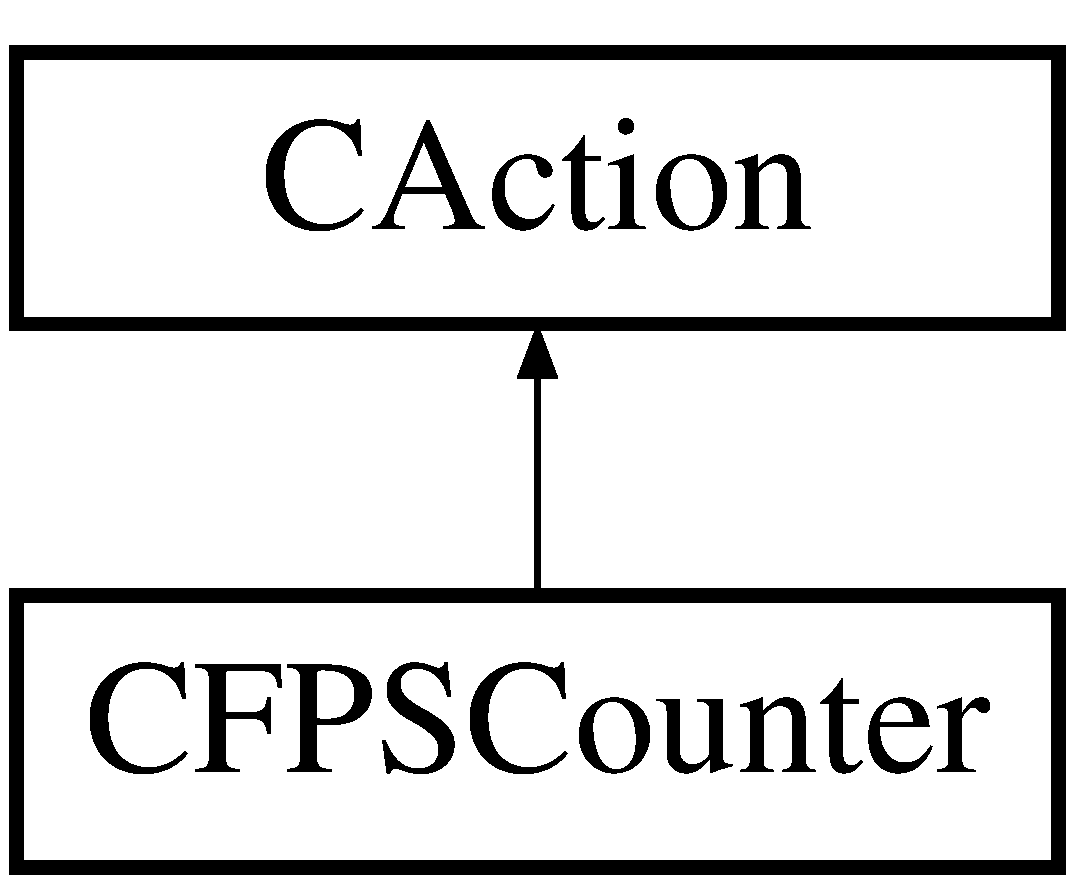
\includegraphics[height=2.000000cm]{class_c_f_p_s_counter}
\end{center}
\end{figure}
\subsection*{公開メンバ関数}
\begin{DoxyCompactItemize}
\item 
\hyperlink{class_c_f_p_s_counter_a2529e1d7efc77fe1c24f9161bae4eab4}{C\+F\+P\+S\+Counter} (U32 \+\_\+u\+Act\+Lv, U32 \+\_\+u\+Sample\+Num)
\begin{DoxyCompactList}\small\item\em コンストラクタ。 \end{DoxyCompactList}\item 
virtual \hyperlink{class_c_f_p_s_counter_a58e43daf84e7df4964508f43d55038f3}{$\sim$\+C\+F\+P\+S\+Counter} ()
\begin{DoxyCompactList}\small\item\em デストラクタ。 \end{DoxyCompactList}\item 
void \hyperlink{class_c_f_p_s_counter_acc82281b59837fb8378cbd5ef8941072}{Action} ()
\begin{DoxyCompactList}\small\item\em 更新処理。 \end{DoxyCompactList}\item 
F32 \hyperlink{class_c_f_p_s_counter_a2ac0a4c5774a5208b6af18f31c7dcddf}{Get\+F\+P\+S} () const 
\begin{DoxyCompactList}\small\item\em F\+P\+Sを取得。 \end{DoxyCompactList}\end{DoxyCompactItemize}
\subsection*{非公開変数類}
\begin{DoxyCompactItemize}
\item 
U32 \hyperlink{class_c_f_p_s_counter_a345278d70add89b57165f4c11b28410a}{m\+\_\+u\+Sample\+Num}
\item 
\hyperlink{_list_8h_a13611c3f3705beb7fa6457d5254bb35f}{C\+List}$<$ U32 $>$ \hyperlink{class_c_f_p_s_counter_a3bc8b67ee009e6480edbbdddabbbdc71}{m\+\_\+c\+Time\+Frame\+List}
\item 
U32 \hyperlink{class_c_f_p_s_counter_a0f8e3c1f1555dc826e73d39fd8d6539a}{m\+\_\+u\+Time\+Total}
\item 
U32 \hyperlink{class_c_f_p_s_counter_a1c5d70cbc932c76ba74d5706ffb015f9}{m\+\_\+u\+Time\+Prev}
\item 
F32 \hyperlink{class_c_f_p_s_counter_a0bc4d470c3de0b1aff04acc6f08b1284}{m\+\_\+f\+F\+P\+S}
\end{DoxyCompactItemize}
\subsection*{その他の継承メンバ}


\subsection{構築子と解体子}
\hypertarget{class_c_f_p_s_counter_a2529e1d7efc77fe1c24f9161bae4eab4}{}\index{C\+F\+P\+S\+Counter@{C\+F\+P\+S\+Counter}!C\+F\+P\+S\+Counter@{C\+F\+P\+S\+Counter}}
\index{C\+F\+P\+S\+Counter@{C\+F\+P\+S\+Counter}!C\+F\+P\+S\+Counter@{C\+F\+P\+S\+Counter}}
\subsubsection[{C\+F\+P\+S\+Counter(\+U32 \+\_\+u\+Act\+Lv, U32 \+\_\+u\+Sample\+Num)}]{\setlength{\rightskip}{0pt plus 5cm}C\+F\+P\+S\+Counter\+::\+C\+F\+P\+S\+Counter (
\begin{DoxyParamCaption}
\item[{U32}]{\+\_\+u\+Act\+Lv, }
\item[{U32}]{\+\_\+u\+Sample\+Num}
\end{DoxyParamCaption}
)}\label{class_c_f_p_s_counter_a2529e1d7efc77fe1c24f9161bae4eab4}


コンストラクタ。 


\begin{DoxyParams}[1]{引数}
\mbox{\tt in}  & {\em \+\_\+u\+Act\+Lv} & \+: アクションレベル。 \\
\hline
\mbox{\tt in}  & {\em \+\_\+u\+Sample\+Num} & \+: F\+P\+Sを計算する際のサンプル数。 \\
\hline
\end{DoxyParams}
\hypertarget{class_c_f_p_s_counter_a58e43daf84e7df4964508f43d55038f3}{}\index{C\+F\+P\+S\+Counter@{C\+F\+P\+S\+Counter}!````~C\+F\+P\+S\+Counter@{$\sim$\+C\+F\+P\+S\+Counter}}
\index{````~C\+F\+P\+S\+Counter@{$\sim$\+C\+F\+P\+S\+Counter}!C\+F\+P\+S\+Counter@{C\+F\+P\+S\+Counter}}
\subsubsection[{$\sim$\+C\+F\+P\+S\+Counter()}]{\setlength{\rightskip}{0pt plus 5cm}virtual C\+F\+P\+S\+Counter\+::$\sim$\+C\+F\+P\+S\+Counter (
\begin{DoxyParamCaption}
{}
\end{DoxyParamCaption}
)\hspace{0.3cm}{\ttfamily [inline]}, {\ttfamily [virtual]}}\label{class_c_f_p_s_counter_a58e43daf84e7df4964508f43d55038f3}


デストラクタ。 



\subsection{関数詳解}
\hypertarget{class_c_f_p_s_counter_acc82281b59837fb8378cbd5ef8941072}{}\index{C\+F\+P\+S\+Counter@{C\+F\+P\+S\+Counter}!Action@{Action}}
\index{Action@{Action}!C\+F\+P\+S\+Counter@{C\+F\+P\+S\+Counter}}
\subsubsection[{Action()}]{\setlength{\rightskip}{0pt plus 5cm}void C\+F\+P\+S\+Counter\+::\+Action (
\begin{DoxyParamCaption}
{}
\end{DoxyParamCaption}
)\hspace{0.3cm}{\ttfamily [virtual]}}\label{class_c_f_p_s_counter_acc82281b59837fb8378cbd5ef8941072}


更新処理。 



\hyperlink{class_c_action_a3fcc5cc0fde844c5cb6e50f7eec9da3c}{C\+Action}を再実装しています。

\hypertarget{class_c_f_p_s_counter_a2ac0a4c5774a5208b6af18f31c7dcddf}{}\index{C\+F\+P\+S\+Counter@{C\+F\+P\+S\+Counter}!Get\+F\+P\+S@{Get\+F\+P\+S}}
\index{Get\+F\+P\+S@{Get\+F\+P\+S}!C\+F\+P\+S\+Counter@{C\+F\+P\+S\+Counter}}
\subsubsection[{Get\+F\+P\+S() const }]{\setlength{\rightskip}{0pt plus 5cm}F32 C\+F\+P\+S\+Counter\+::\+Get\+F\+P\+S (
\begin{DoxyParamCaption}
{}
\end{DoxyParamCaption}
) const\hspace{0.3cm}{\ttfamily [inline]}}\label{class_c_f_p_s_counter_a2ac0a4c5774a5208b6af18f31c7dcddf}


F\+P\+Sを取得。 



\subsection{メンバ詳解}
\hypertarget{class_c_f_p_s_counter_a3bc8b67ee009e6480edbbdddabbbdc71}{}\index{C\+F\+P\+S\+Counter@{C\+F\+P\+S\+Counter}!m\+\_\+c\+Time\+Frame\+List@{m\+\_\+c\+Time\+Frame\+List}}
\index{m\+\_\+c\+Time\+Frame\+List@{m\+\_\+c\+Time\+Frame\+List}!C\+F\+P\+S\+Counter@{C\+F\+P\+S\+Counter}}
\subsubsection[{m\+\_\+c\+Time\+Frame\+List}]{\setlength{\rightskip}{0pt plus 5cm}{\bf C\+List}$<$U32$>$ C\+F\+P\+S\+Counter\+::m\+\_\+c\+Time\+Frame\+List\hspace{0.3cm}{\ttfamily [private]}}\label{class_c_f_p_s_counter_a3bc8b67ee009e6480edbbdddabbbdc71}
\hypertarget{class_c_f_p_s_counter_a0bc4d470c3de0b1aff04acc6f08b1284}{}\index{C\+F\+P\+S\+Counter@{C\+F\+P\+S\+Counter}!m\+\_\+f\+F\+P\+S@{m\+\_\+f\+F\+P\+S}}
\index{m\+\_\+f\+F\+P\+S@{m\+\_\+f\+F\+P\+S}!C\+F\+P\+S\+Counter@{C\+F\+P\+S\+Counter}}
\subsubsection[{m\+\_\+f\+F\+P\+S}]{\setlength{\rightskip}{0pt plus 5cm}F32 C\+F\+P\+S\+Counter\+::m\+\_\+f\+F\+P\+S\hspace{0.3cm}{\ttfamily [private]}}\label{class_c_f_p_s_counter_a0bc4d470c3de0b1aff04acc6f08b1284}
\hypertarget{class_c_f_p_s_counter_a345278d70add89b57165f4c11b28410a}{}\index{C\+F\+P\+S\+Counter@{C\+F\+P\+S\+Counter}!m\+\_\+u\+Sample\+Num@{m\+\_\+u\+Sample\+Num}}
\index{m\+\_\+u\+Sample\+Num@{m\+\_\+u\+Sample\+Num}!C\+F\+P\+S\+Counter@{C\+F\+P\+S\+Counter}}
\subsubsection[{m\+\_\+u\+Sample\+Num}]{\setlength{\rightskip}{0pt plus 5cm}U32 C\+F\+P\+S\+Counter\+::m\+\_\+u\+Sample\+Num\hspace{0.3cm}{\ttfamily [private]}}\label{class_c_f_p_s_counter_a345278d70add89b57165f4c11b28410a}
\hypertarget{class_c_f_p_s_counter_a1c5d70cbc932c76ba74d5706ffb015f9}{}\index{C\+F\+P\+S\+Counter@{C\+F\+P\+S\+Counter}!m\+\_\+u\+Time\+Prev@{m\+\_\+u\+Time\+Prev}}
\index{m\+\_\+u\+Time\+Prev@{m\+\_\+u\+Time\+Prev}!C\+F\+P\+S\+Counter@{C\+F\+P\+S\+Counter}}
\subsubsection[{m\+\_\+u\+Time\+Prev}]{\setlength{\rightskip}{0pt plus 5cm}U32 C\+F\+P\+S\+Counter\+::m\+\_\+u\+Time\+Prev\hspace{0.3cm}{\ttfamily [private]}}\label{class_c_f_p_s_counter_a1c5d70cbc932c76ba74d5706ffb015f9}
\hypertarget{class_c_f_p_s_counter_a0f8e3c1f1555dc826e73d39fd8d6539a}{}\index{C\+F\+P\+S\+Counter@{C\+F\+P\+S\+Counter}!m\+\_\+u\+Time\+Total@{m\+\_\+u\+Time\+Total}}
\index{m\+\_\+u\+Time\+Total@{m\+\_\+u\+Time\+Total}!C\+F\+P\+S\+Counter@{C\+F\+P\+S\+Counter}}
\subsubsection[{m\+\_\+u\+Time\+Total}]{\setlength{\rightskip}{0pt plus 5cm}U32 C\+F\+P\+S\+Counter\+::m\+\_\+u\+Time\+Total\hspace{0.3cm}{\ttfamily [private]}}\label{class_c_f_p_s_counter_a0f8e3c1f1555dc826e73d39fd8d6539a}


このクラス詳解は次のファイルから抽出されました\+:\begin{DoxyCompactItemize}
\item 
D\+:/\+Project/\+Game/\+Lib/\+Debug/\hyperlink{_f_p_s_counter_8h}{F\+P\+S\+Counter.\+h}\item 
D\+:/\+Project/\+Game/\+Lib/\+Debug/\hyperlink{_f_p_s_counter_8cpp}{F\+P\+S\+Counter.\+cpp}\end{DoxyCompactItemize}

\hypertarget{class_c_f_p_s_viewer}{}\section{C\+F\+P\+S\+Viewer クラス}
\label{class_c_f_p_s_viewer}\index{C\+F\+P\+S\+Viewer@{C\+F\+P\+S\+Viewer}}


{\ttfamily \#include $<$F\+P\+S\+Viewer.\+h$>$}

C\+F\+P\+S\+Viewer の継承関係図\begin{figure}[H]
\begin{center}
\leavevmode
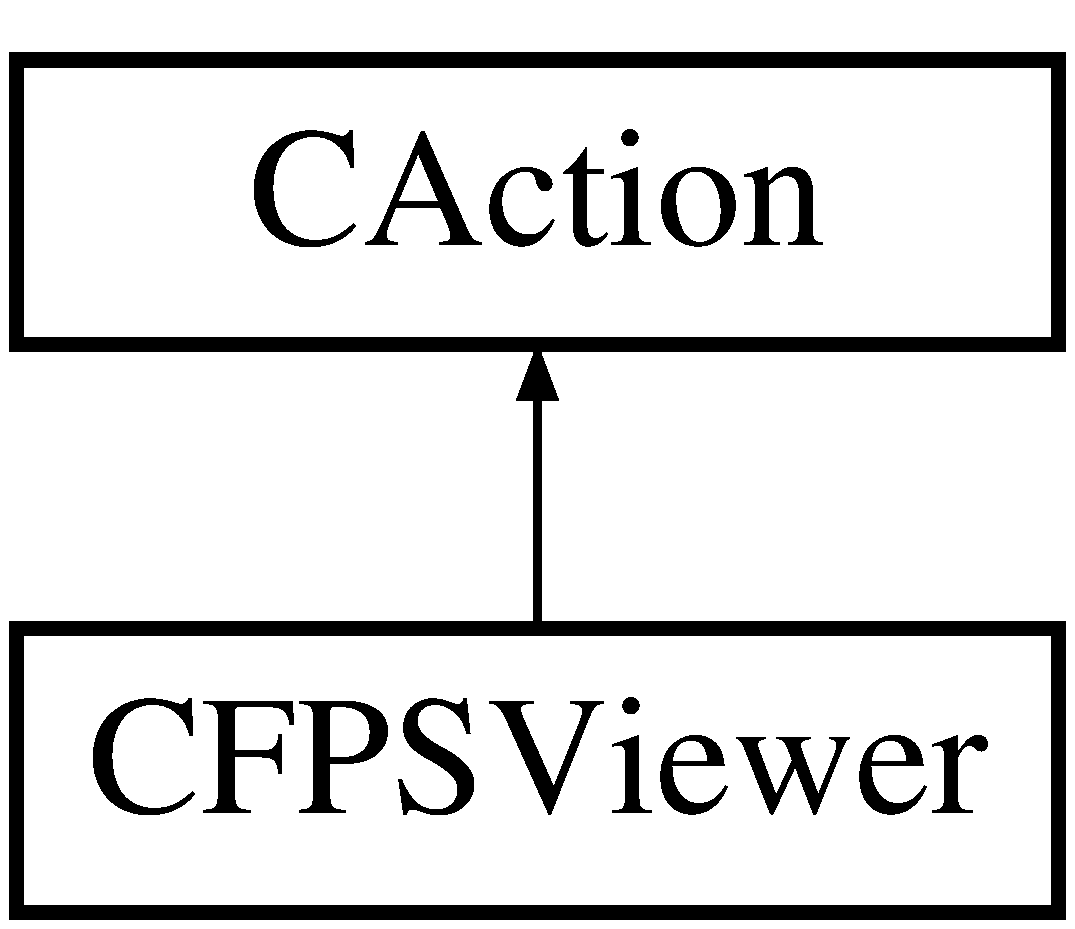
\includegraphics[height=2.000000cm]{class_c_f_p_s_viewer}
\end{center}
\end{figure}
\subsection*{公開メンバ関数}
\begin{DoxyCompactItemize}
\item 
\hyperlink{class_c_f_p_s_viewer_aee0922eb44152f58586245862a66586e}{C\+F\+P\+S\+Viewer} (H\+W\+N\+D \+\_\+h\+Wnd, U32 \+\_\+u\+Action\+Lv)
\begin{DoxyCompactList}\small\item\em コンストラクタ。 \end{DoxyCompactList}\item 
virtual \hyperlink{class_c_f_p_s_viewer_a98af679a51ac2947e8d7a232321b1abc}{$\sim$\+C\+F\+P\+S\+Viewer} ()
\begin{DoxyCompactList}\small\item\em デストラクタ。 \end{DoxyCompactList}\item 
virtual void \hyperlink{class_c_f_p_s_viewer_abde661517b45dbe7cd19a86ef8a0b2af}{Action} () override
\begin{DoxyCompactList}\small\item\em 更新処理。 \end{DoxyCompactList}\end{DoxyCompactItemize}
\subsection*{非公開変数類}
\begin{DoxyCompactItemize}
\item 
H\+W\+N\+D \hyperlink{class_c_f_p_s_viewer_a096208af929712b964e2c80fe70da6f6}{m\+\_\+h\+Wnd}
\item 
\hyperlink{class_c_f_p_s_counter}{C\+F\+P\+S\+Counter} $\ast$ \hyperlink{class_c_f_p_s_viewer_a33af8585644a97027e76133aefcec5fb}{m\+\_\+pc\+F\+P\+S\+Counter}
\begin{DoxyCompactList}\small\item\em F\+P\+S計測クラス。 \end{DoxyCompactList}\end{DoxyCompactItemize}
\subsection*{その他の継承メンバ}


\subsection{構築子と解体子}
\hypertarget{class_c_f_p_s_viewer_aee0922eb44152f58586245862a66586e}{}\index{C\+F\+P\+S\+Viewer@{C\+F\+P\+S\+Viewer}!C\+F\+P\+S\+Viewer@{C\+F\+P\+S\+Viewer}}
\index{C\+F\+P\+S\+Viewer@{C\+F\+P\+S\+Viewer}!C\+F\+P\+S\+Viewer@{C\+F\+P\+S\+Viewer}}
\subsubsection[{C\+F\+P\+S\+Viewer(\+H\+W\+N\+D \+\_\+h\+Wnd, U32 \+\_\+u\+Action\+Lv)}]{\setlength{\rightskip}{0pt plus 5cm}C\+F\+P\+S\+Viewer\+::\+C\+F\+P\+S\+Viewer (
\begin{DoxyParamCaption}
\item[{H\+W\+N\+D}]{\+\_\+h\+Wnd, }
\item[{U32}]{\+\_\+u\+Action\+Lv}
\end{DoxyParamCaption}
)}\label{class_c_f_p_s_viewer_aee0922eb44152f58586245862a66586e}


コンストラクタ。 


\begin{DoxyParams}[1]{引数}
\mbox{\tt in}  & {\em \+\_\+h\+Wnd} & \+: ウィンドウハンドル。 \\
\hline
\mbox{\tt in}  & {\em \+\_\+u\+Actiuon\+Lv} & \+: アクションレベル。 \\
\hline
\end{DoxyParams}
\hypertarget{class_c_f_p_s_viewer_a98af679a51ac2947e8d7a232321b1abc}{}\index{C\+F\+P\+S\+Viewer@{C\+F\+P\+S\+Viewer}!````~C\+F\+P\+S\+Viewer@{$\sim$\+C\+F\+P\+S\+Viewer}}
\index{````~C\+F\+P\+S\+Viewer@{$\sim$\+C\+F\+P\+S\+Viewer}!C\+F\+P\+S\+Viewer@{C\+F\+P\+S\+Viewer}}
\subsubsection[{$\sim$\+C\+F\+P\+S\+Viewer()}]{\setlength{\rightskip}{0pt plus 5cm}C\+F\+P\+S\+Viewer\+::$\sim$\+C\+F\+P\+S\+Viewer (
\begin{DoxyParamCaption}
{}
\end{DoxyParamCaption}
)\hspace{0.3cm}{\ttfamily [virtual]}}\label{class_c_f_p_s_viewer_a98af679a51ac2947e8d7a232321b1abc}


デストラクタ。 



\subsection{関数詳解}
\hypertarget{class_c_f_p_s_viewer_abde661517b45dbe7cd19a86ef8a0b2af}{}\index{C\+F\+P\+S\+Viewer@{C\+F\+P\+S\+Viewer}!Action@{Action}}
\index{Action@{Action}!C\+F\+P\+S\+Viewer@{C\+F\+P\+S\+Viewer}}
\subsubsection[{Action() override}]{\setlength{\rightskip}{0pt plus 5cm}void C\+F\+P\+S\+Viewer\+::\+Action (
\begin{DoxyParamCaption}
{}
\end{DoxyParamCaption}
)\hspace{0.3cm}{\ttfamily [override]}, {\ttfamily [virtual]}}\label{class_c_f_p_s_viewer_abde661517b45dbe7cd19a86ef8a0b2af}


更新処理。 



\hyperlink{class_c_action_a3fcc5cc0fde844c5cb6e50f7eec9da3c}{C\+Action}を再実装しています。



\subsection{メンバ詳解}
\hypertarget{class_c_f_p_s_viewer_a096208af929712b964e2c80fe70da6f6}{}\index{C\+F\+P\+S\+Viewer@{C\+F\+P\+S\+Viewer}!m\+\_\+h\+Wnd@{m\+\_\+h\+Wnd}}
\index{m\+\_\+h\+Wnd@{m\+\_\+h\+Wnd}!C\+F\+P\+S\+Viewer@{C\+F\+P\+S\+Viewer}}
\subsubsection[{m\+\_\+h\+Wnd}]{\setlength{\rightskip}{0pt plus 5cm}H\+W\+N\+D C\+F\+P\+S\+Viewer\+::m\+\_\+h\+Wnd\hspace{0.3cm}{\ttfamily [private]}}\label{class_c_f_p_s_viewer_a096208af929712b964e2c80fe70da6f6}
\hypertarget{class_c_f_p_s_viewer_a33af8585644a97027e76133aefcec5fb}{}\index{C\+F\+P\+S\+Viewer@{C\+F\+P\+S\+Viewer}!m\+\_\+pc\+F\+P\+S\+Counter@{m\+\_\+pc\+F\+P\+S\+Counter}}
\index{m\+\_\+pc\+F\+P\+S\+Counter@{m\+\_\+pc\+F\+P\+S\+Counter}!C\+F\+P\+S\+Viewer@{C\+F\+P\+S\+Viewer}}
\subsubsection[{m\+\_\+pc\+F\+P\+S\+Counter}]{\setlength{\rightskip}{0pt plus 5cm}{\bf C\+F\+P\+S\+Counter}$\ast$ C\+F\+P\+S\+Viewer\+::m\+\_\+pc\+F\+P\+S\+Counter\hspace{0.3cm}{\ttfamily [private]}}\label{class_c_f_p_s_viewer_a33af8585644a97027e76133aefcec5fb}


F\+P\+S計測クラス。 



このクラス詳解は次のファイルから抽出されました\+:\begin{DoxyCompactItemize}
\item 
D\+:/\+Project/\+Game/\+Lib/\+Debug/\hyperlink{_f_p_s_viewer_8h}{F\+P\+S\+Viewer.\+h}\item 
D\+:/\+Project/\+Game/\+Lib/\+Debug/\hyperlink{_f_p_s_viewer_8cpp}{F\+P\+S\+Viewer.\+cpp}\end{DoxyCompactItemize}

\hypertarget{class_c_game_sequence_factory}{}\section{C\+Game\+Sequence\+Factory クラス}
\label{class_c_game_sequence_factory}\index{C\+Game\+Sequence\+Factory@{C\+Game\+Sequence\+Factory}}


{\ttfamily \#include $<$Game\+Sequence\+Factory.\+h$>$}

C\+Game\+Sequence\+Factory の継承関係図\begin{figure}[H]
\begin{center}
\leavevmode
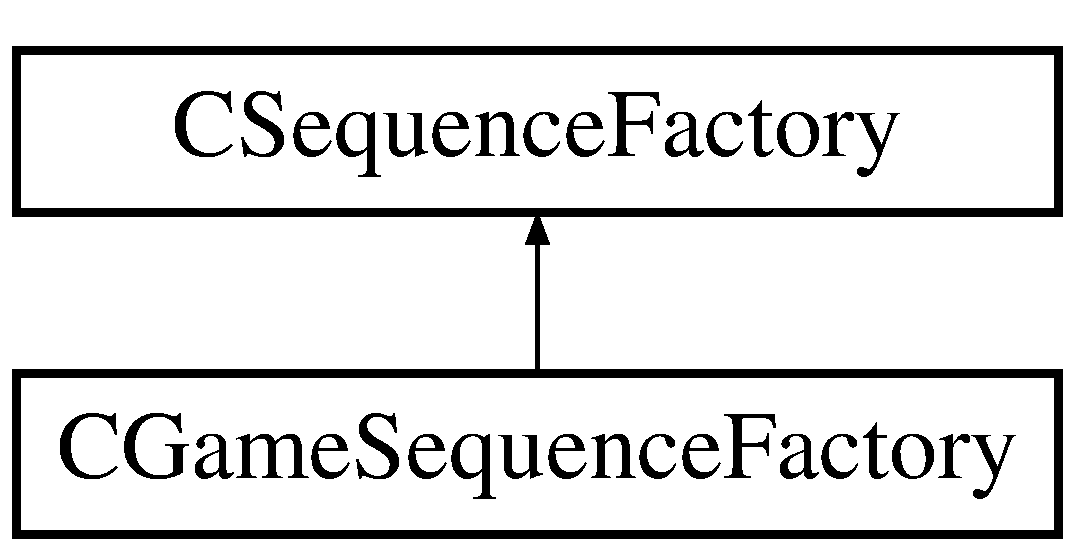
\includegraphics[height=2.000000cm]{class_c_game_sequence_factory}
\end{center}
\end{figure}
\subsection*{公開メンバ関数}
\begin{DoxyCompactItemize}
\item 
\hyperlink{class_c_game_sequence_factory_a8ee16d920fba7096edf2dbbb6d451b90}{C\+Game\+Sequence\+Factory} ()
\begin{DoxyCompactList}\small\item\em コンストラクタ。 \end{DoxyCompactList}\item 
virtual \hyperlink{class_c_game_sequence_factory_aff2ca8de400e77e24f59a1748e515187}{$\sim$\+C\+Game\+Sequence\+Factory} ()
\begin{DoxyCompactList}\small\item\em デストラクタ。 \end{DoxyCompactList}\item 
virtual \hyperlink{class_c_sequence}{C\+Sequence} $\ast$ \hyperlink{class_c_game_sequence_factory_a868862261fd54f2d6f05a7fd0ba41b34}{Create\+Instance} (U32 \+\_\+u\+Sequence\+I\+D) override
\begin{DoxyCompactList}\small\item\em シーケンスを生成。 \end{DoxyCompactList}\end{DoxyCompactItemize}


\subsection{構築子と解体子}
\hypertarget{class_c_game_sequence_factory_a8ee16d920fba7096edf2dbbb6d451b90}{}\index{C\+Game\+Sequence\+Factory@{C\+Game\+Sequence\+Factory}!C\+Game\+Sequence\+Factory@{C\+Game\+Sequence\+Factory}}
\index{C\+Game\+Sequence\+Factory@{C\+Game\+Sequence\+Factory}!C\+Game\+Sequence\+Factory@{C\+Game\+Sequence\+Factory}}
\subsubsection[{C\+Game\+Sequence\+Factory()}]{\setlength{\rightskip}{0pt plus 5cm}C\+Game\+Sequence\+Factory\+::\+C\+Game\+Sequence\+Factory (
\begin{DoxyParamCaption}
{}
\end{DoxyParamCaption}
)\hspace{0.3cm}{\ttfamily [inline]}}\label{class_c_game_sequence_factory_a8ee16d920fba7096edf2dbbb6d451b90}


コンストラクタ。 

\hypertarget{class_c_game_sequence_factory_aff2ca8de400e77e24f59a1748e515187}{}\index{C\+Game\+Sequence\+Factory@{C\+Game\+Sequence\+Factory}!````~C\+Game\+Sequence\+Factory@{$\sim$\+C\+Game\+Sequence\+Factory}}
\index{````~C\+Game\+Sequence\+Factory@{$\sim$\+C\+Game\+Sequence\+Factory}!C\+Game\+Sequence\+Factory@{C\+Game\+Sequence\+Factory}}
\subsubsection[{$\sim$\+C\+Game\+Sequence\+Factory()}]{\setlength{\rightskip}{0pt plus 5cm}virtual C\+Game\+Sequence\+Factory\+::$\sim$\+C\+Game\+Sequence\+Factory (
\begin{DoxyParamCaption}
{}
\end{DoxyParamCaption}
)\hspace{0.3cm}{\ttfamily [inline]}, {\ttfamily [virtual]}}\label{class_c_game_sequence_factory_aff2ca8de400e77e24f59a1748e515187}


デストラクタ。 



\subsection{関数詳解}
\hypertarget{class_c_game_sequence_factory_a868862261fd54f2d6f05a7fd0ba41b34}{}\index{C\+Game\+Sequence\+Factory@{C\+Game\+Sequence\+Factory}!Create\+Instance@{Create\+Instance}}
\index{Create\+Instance@{Create\+Instance}!C\+Game\+Sequence\+Factory@{C\+Game\+Sequence\+Factory}}
\subsubsection[{Create\+Instance(\+U32 \+\_\+u\+Sequence\+I\+D) override}]{\setlength{\rightskip}{0pt plus 5cm}{\bf C\+Sequence} $\ast$ C\+Game\+Sequence\+Factory\+::\+Create\+Instance (
\begin{DoxyParamCaption}
\item[{U32}]{\+\_\+u\+Sequence\+I\+D}
\end{DoxyParamCaption}
)\hspace{0.3cm}{\ttfamily [override]}, {\ttfamily [virtual]}}\label{class_c_game_sequence_factory_a868862261fd54f2d6f05a7fd0ba41b34}


シーケンスを生成。 

シーケンスを作成。


\begin{DoxyParams}[1]{引数}
\mbox{\tt in}  & {\em \+\_\+u\+Sequence\+I\+D} & \+: シーケンス\+I\+D( En\+Sequence\+I\+D ) \\
\hline
\end{DoxyParams}

\begin{DoxyRetVals}{戻り値}
{\em シーケンスのインスタンス。} & \\
\hline
\end{DoxyRetVals}


\hyperlink{class_c_sequence_factory_aba3a273d0da93264b7d18e43d86d4c39}{C\+Sequence\+Factory}を再実装しています。



このクラス詳解は次のファイルから抽出されました\+:\begin{DoxyCompactItemize}
\item 
D\+:/\+Project/\+Game/\+Sequence/\hyperlink{_game_sequence_factory_8h}{Game\+Sequence\+Factory.\+h}\item 
D\+:/\+Project/\+Game/\+Sequence/\hyperlink{_game_sequence_factory_8cpp}{Game\+Sequence\+Factory.\+cpp}\end{DoxyCompactItemize}

\hypertarget{class_c_init_sequence}{}\section{C\+Init\+Sequence クラス}
\label{class_c_init_sequence}\index{C\+Init\+Sequence@{C\+Init\+Sequence}}


{\ttfamily \#include $<$Init\+Sequence.\+h$>$}

C\+Init\+Sequence の継承関係図\begin{figure}[H]
\begin{center}
\leavevmode
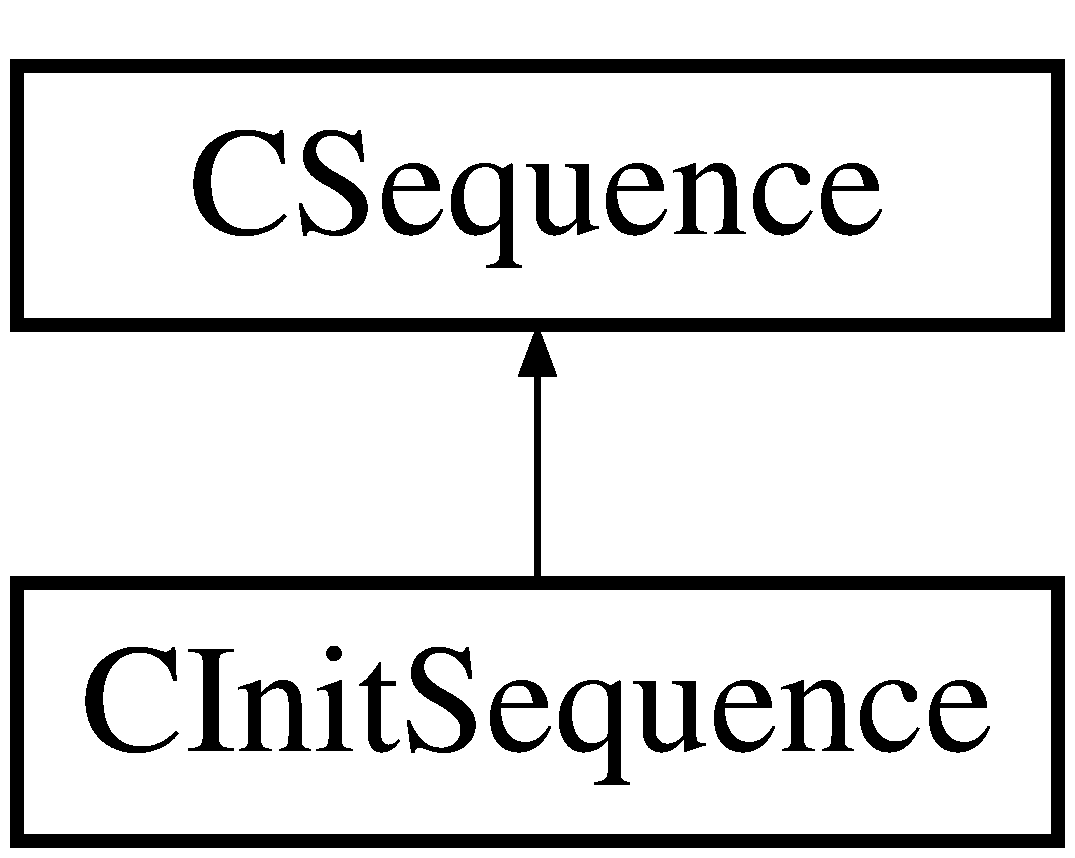
\includegraphics[height=2.000000cm]{class_c_init_sequence}
\end{center}
\end{figure}
\subsection*{公開メンバ関数}
\begin{DoxyCompactItemize}
\item 
\hyperlink{class_c_init_sequence_a29e4587c31c2ae19ef9cd646973bbeba}{C\+Init\+Sequence} ()
\begin{DoxyCompactList}\small\item\em コンストラクタ。 \end{DoxyCompactList}\item 
virtual \hyperlink{class_c_init_sequence_abc416fc4b10a9421767a0e5ce923d67a}{$\sim$\+C\+Init\+Sequence} ()
\begin{DoxyCompactList}\small\item\em デストラクタ。 \end{DoxyCompactList}\item 
void \hyperlink{class_c_init_sequence_a52cb5822b6f2c281f3969fadc61a47fb}{Loop\+Start\+Act} () override
\begin{DoxyCompactList}\small\item\em フレーム開始時の処理。 \end{DoxyCompactList}\item 
void \hyperlink{class_c_init_sequence_aae10f421cc1738b571022d2bdc3898d0}{Loop\+End\+Act} () override
\begin{DoxyCompactList}\small\item\em フレーム終了時の処理。 \end{DoxyCompactList}\item 
bool \hyperlink{class_c_init_sequence_ac837c22aeab7e9c10f3f9a217390661c}{Is\+End} () const  override
\begin{DoxyCompactList}\small\item\em 終了したか。 \end{DoxyCompactList}\item 
U32 \hyperlink{class_c_init_sequence_a7d4aec0184771958424f2234716a4945}{Get\+Next} () const  override
\begin{DoxyCompactList}\small\item\em 次のシーケンスを取得。 \end{DoxyCompactList}\end{DoxyCompactItemize}
\subsection*{非公開変数類}
\begin{DoxyCompactItemize}
\item 
\hyperlink{class_c_p_m_d_reader}{C\+P\+M\+D\+Reader} $\ast$ \hyperlink{class_c_init_sequence_acb2968a68f82f21b579371f0d2533863}{m\+\_\+pc\+P\+M\+D\+Reader}
\item 
\hyperlink{class_c_p_m_d_mesh}{C\+P\+M\+D\+Mesh} $\ast$ \hyperlink{class_c_init_sequence_a2a6637e5348a20fe286258e723b85d31}{m\+\_\+pc\+Mesh}
\item 
\hyperlink{class_c_mesh_drawer}{C\+Mesh\+Drawer} $\ast$ \hyperlink{class_c_init_sequence_a7581fe58f808b9490a8d65e026fd334e}{m\+\_\+pc\+Mesh\+Drawer}
\end{DoxyCompactItemize}


\subsection{構築子と解体子}
\hypertarget{class_c_init_sequence_a29e4587c31c2ae19ef9cd646973bbeba}{}\index{C\+Init\+Sequence@{C\+Init\+Sequence}!C\+Init\+Sequence@{C\+Init\+Sequence}}
\index{C\+Init\+Sequence@{C\+Init\+Sequence}!C\+Init\+Sequence@{C\+Init\+Sequence}}
\subsubsection[{C\+Init\+Sequence()}]{\setlength{\rightskip}{0pt plus 5cm}C\+Init\+Sequence\+::\+C\+Init\+Sequence (
\begin{DoxyParamCaption}
{}
\end{DoxyParamCaption}
)\hspace{0.3cm}{\ttfamily [inline]}}\label{class_c_init_sequence_a29e4587c31c2ae19ef9cd646973bbeba}


コンストラクタ。 

\hypertarget{class_c_init_sequence_abc416fc4b10a9421767a0e5ce923d67a}{}\index{C\+Init\+Sequence@{C\+Init\+Sequence}!````~C\+Init\+Sequence@{$\sim$\+C\+Init\+Sequence}}
\index{````~C\+Init\+Sequence@{$\sim$\+C\+Init\+Sequence}!C\+Init\+Sequence@{C\+Init\+Sequence}}
\subsubsection[{$\sim$\+C\+Init\+Sequence()}]{\setlength{\rightskip}{0pt plus 5cm}virtual C\+Init\+Sequence\+::$\sim$\+C\+Init\+Sequence (
\begin{DoxyParamCaption}
{}
\end{DoxyParamCaption}
)\hspace{0.3cm}{\ttfamily [inline]}, {\ttfamily [virtual]}}\label{class_c_init_sequence_abc416fc4b10a9421767a0e5ce923d67a}


デストラクタ。 



\subsection{関数詳解}
\hypertarget{class_c_init_sequence_a7d4aec0184771958424f2234716a4945}{}\index{C\+Init\+Sequence@{C\+Init\+Sequence}!Get\+Next@{Get\+Next}}
\index{Get\+Next@{Get\+Next}!C\+Init\+Sequence@{C\+Init\+Sequence}}
\subsubsection[{Get\+Next() const  override}]{\setlength{\rightskip}{0pt plus 5cm}U32 C\+Init\+Sequence\+::\+Get\+Next (
\begin{DoxyParamCaption}
{}
\end{DoxyParamCaption}
) const\hspace{0.3cm}{\ttfamily [inline]}, {\ttfamily [override]}, {\ttfamily [virtual]}}\label{class_c_init_sequence_a7d4aec0184771958424f2234716a4945}


次のシーケンスを取得。 



\hyperlink{class_c_sequence_a9819cf065c49e5a8bee7f04f62d37d16}{C\+Sequence}を実装しています。

\hypertarget{class_c_init_sequence_ac837c22aeab7e9c10f3f9a217390661c}{}\index{C\+Init\+Sequence@{C\+Init\+Sequence}!Is\+End@{Is\+End}}
\index{Is\+End@{Is\+End}!C\+Init\+Sequence@{C\+Init\+Sequence}}
\subsubsection[{Is\+End() const  override}]{\setlength{\rightskip}{0pt plus 5cm}bool C\+Init\+Sequence\+::\+Is\+End (
\begin{DoxyParamCaption}
{}
\end{DoxyParamCaption}
) const\hspace{0.3cm}{\ttfamily [inline]}, {\ttfamily [override]}, {\ttfamily [virtual]}}\label{class_c_init_sequence_ac837c22aeab7e9c10f3f9a217390661c}


終了したか。 



\hyperlink{class_c_sequence_acec92faef8ee677063980776b4c242a1}{C\+Sequence}を実装しています。

\hypertarget{class_c_init_sequence_aae10f421cc1738b571022d2bdc3898d0}{}\index{C\+Init\+Sequence@{C\+Init\+Sequence}!Loop\+End\+Act@{Loop\+End\+Act}}
\index{Loop\+End\+Act@{Loop\+End\+Act}!C\+Init\+Sequence@{C\+Init\+Sequence}}
\subsubsection[{Loop\+End\+Act() override}]{\setlength{\rightskip}{0pt plus 5cm}void C\+Init\+Sequence\+::\+Loop\+End\+Act (
\begin{DoxyParamCaption}
{}
\end{DoxyParamCaption}
)\hspace{0.3cm}{\ttfamily [inline]}, {\ttfamily [override]}, {\ttfamily [virtual]}}\label{class_c_init_sequence_aae10f421cc1738b571022d2bdc3898d0}


フレーム終了時の処理。 



\hyperlink{class_c_sequence_a0a2f5146bf33a4bd8c480d9da5a0538d}{C\+Sequence}を再実装しています。

\hypertarget{class_c_init_sequence_a52cb5822b6f2c281f3969fadc61a47fb}{}\index{C\+Init\+Sequence@{C\+Init\+Sequence}!Loop\+Start\+Act@{Loop\+Start\+Act}}
\index{Loop\+Start\+Act@{Loop\+Start\+Act}!C\+Init\+Sequence@{C\+Init\+Sequence}}
\subsubsection[{Loop\+Start\+Act() override}]{\setlength{\rightskip}{0pt plus 5cm}void C\+Init\+Sequence\+::\+Loop\+Start\+Act (
\begin{DoxyParamCaption}
{}
\end{DoxyParamCaption}
)\hspace{0.3cm}{\ttfamily [inline]}, {\ttfamily [override]}, {\ttfamily [virtual]}}\label{class_c_init_sequence_a52cb5822b6f2c281f3969fadc61a47fb}


フレーム開始時の処理。 



\hyperlink{class_c_sequence_a0124977c5ae40f9289c7867ff71c743d}{C\+Sequence}を再実装しています。



\subsection{メンバ詳解}
\hypertarget{class_c_init_sequence_a2a6637e5348a20fe286258e723b85d31}{}\index{C\+Init\+Sequence@{C\+Init\+Sequence}!m\+\_\+pc\+Mesh@{m\+\_\+pc\+Mesh}}
\index{m\+\_\+pc\+Mesh@{m\+\_\+pc\+Mesh}!C\+Init\+Sequence@{C\+Init\+Sequence}}
\subsubsection[{m\+\_\+pc\+Mesh}]{\setlength{\rightskip}{0pt plus 5cm}{\bf C\+P\+M\+D\+Mesh}$\ast$ C\+Init\+Sequence\+::m\+\_\+pc\+Mesh\hspace{0.3cm}{\ttfamily [private]}}\label{class_c_init_sequence_a2a6637e5348a20fe286258e723b85d31}
\hypertarget{class_c_init_sequence_a7581fe58f808b9490a8d65e026fd334e}{}\index{C\+Init\+Sequence@{C\+Init\+Sequence}!m\+\_\+pc\+Mesh\+Drawer@{m\+\_\+pc\+Mesh\+Drawer}}
\index{m\+\_\+pc\+Mesh\+Drawer@{m\+\_\+pc\+Mesh\+Drawer}!C\+Init\+Sequence@{C\+Init\+Sequence}}
\subsubsection[{m\+\_\+pc\+Mesh\+Drawer}]{\setlength{\rightskip}{0pt plus 5cm}{\bf C\+Mesh\+Drawer}$\ast$ C\+Init\+Sequence\+::m\+\_\+pc\+Mesh\+Drawer\hspace{0.3cm}{\ttfamily [private]}}\label{class_c_init_sequence_a7581fe58f808b9490a8d65e026fd334e}
\hypertarget{class_c_init_sequence_acb2968a68f82f21b579371f0d2533863}{}\index{C\+Init\+Sequence@{C\+Init\+Sequence}!m\+\_\+pc\+P\+M\+D\+Reader@{m\+\_\+pc\+P\+M\+D\+Reader}}
\index{m\+\_\+pc\+P\+M\+D\+Reader@{m\+\_\+pc\+P\+M\+D\+Reader}!C\+Init\+Sequence@{C\+Init\+Sequence}}
\subsubsection[{m\+\_\+pc\+P\+M\+D\+Reader}]{\setlength{\rightskip}{0pt plus 5cm}{\bf C\+P\+M\+D\+Reader}$\ast$ C\+Init\+Sequence\+::m\+\_\+pc\+P\+M\+D\+Reader\hspace{0.3cm}{\ttfamily [private]}}\label{class_c_init_sequence_acb2968a68f82f21b579371f0d2533863}


このクラス詳解は次のファイルから抽出されました\+:\begin{DoxyCompactItemize}
\item 
D\+:/\+Project/\+Game/\+Title/\hyperlink{_init_sequence_8h}{Init\+Sequence.\+h}\end{DoxyCompactItemize}

\hypertarget{class_c_job}{}\section{C\+Job クラス}
\label{class_c_job}\index{C\+Job@{C\+Job}}


{\ttfamily \#include $<$Job.\+h$>$}

C\+Job の継承関係図\begin{figure}[H]
\begin{center}
\leavevmode
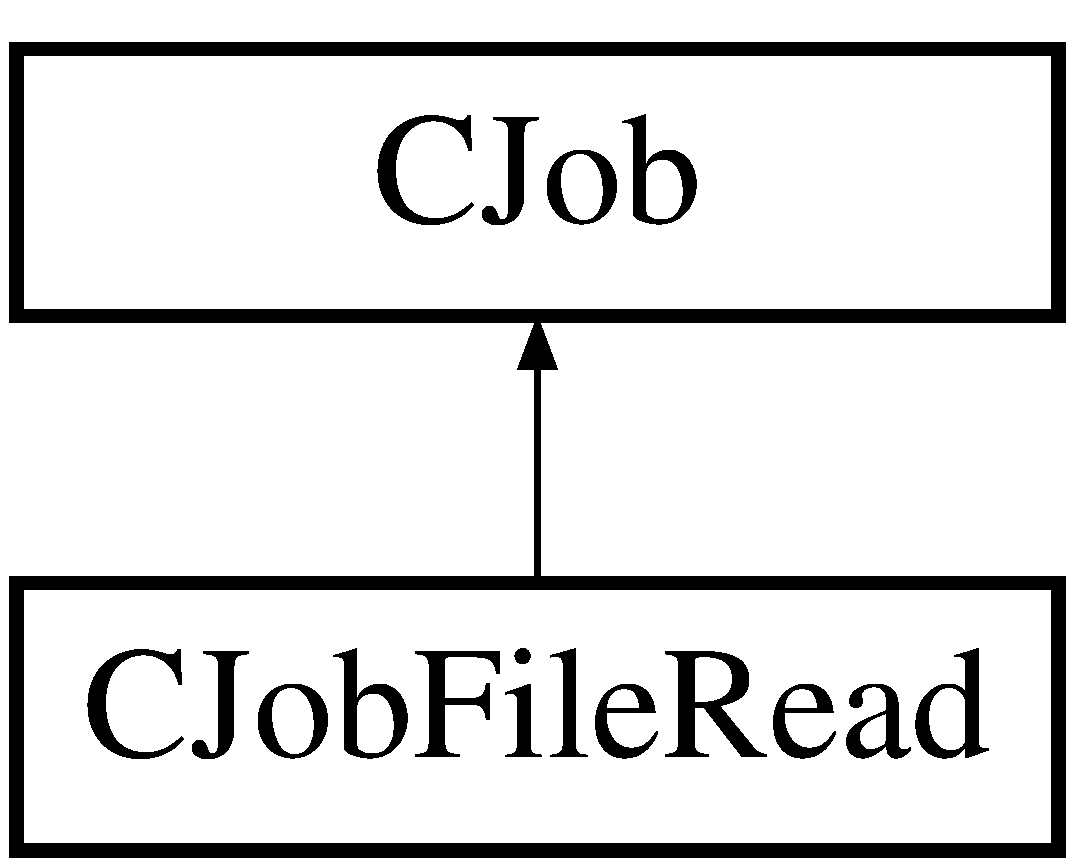
\includegraphics[height=2.000000cm]{class_c_job}
\end{center}
\end{figure}
\subsection*{公開メンバ関数}
\begin{DoxyCompactItemize}
\item 
\hyperlink{class_c_job_ac1e5467251edcba0961d167840efb4a7}{C\+Job} ()
\begin{DoxyCompactList}\small\item\em コンストラクタ。 \end{DoxyCompactList}\item 
virtual \hyperlink{class_c_job_a3aba2e1e742f8af183b403b1dd0aab44}{$\sim$\+C\+Job} ()
\begin{DoxyCompactList}\small\item\em デストラクタ。 \end{DoxyCompactList}\item 
virtual void \hyperlink{class_c_job_af5b3f6138549671f6728bae1113777fe}{Run} ()
\begin{DoxyCompactList}\small\item\em ワーカースレッドで行う処理。 \end{DoxyCompactList}\item 
bool \hyperlink{class_c_job_aebcde411175b14f3347639a39aae1460}{Is\+End} () const 
\begin{DoxyCompactList}\small\item\em 終了したか。 \end{DoxyCompactList}\item 
void \hyperlink{class_c_job_a371cc1b43d7d50b14d10fd55d01638d3}{Set\+End} (bool \+\_\+b\+End)
\begin{DoxyCompactList}\small\item\em 終了したか設定。 \end{DoxyCompactList}\end{DoxyCompactItemize}
\subsection*{非公開変数類}
\begin{DoxyCompactItemize}
\item 
bool \hyperlink{class_c_job_afcf1f1b7b2563cc20a5e2d596f7c06a3}{m\+\_\+b\+End}
\end{DoxyCompactItemize}


\subsection{構築子と解体子}
\hypertarget{class_c_job_ac1e5467251edcba0961d167840efb4a7}{}\index{C\+Job@{C\+Job}!C\+Job@{C\+Job}}
\index{C\+Job@{C\+Job}!C\+Job@{C\+Job}}
\subsubsection[{C\+Job()}]{\setlength{\rightskip}{0pt plus 5cm}C\+Job\+::\+C\+Job (
\begin{DoxyParamCaption}
{}
\end{DoxyParamCaption}
)\hspace{0.3cm}{\ttfamily [inline]}}\label{class_c_job_ac1e5467251edcba0961d167840efb4a7}


コンストラクタ。 

\hypertarget{class_c_job_a3aba2e1e742f8af183b403b1dd0aab44}{}\index{C\+Job@{C\+Job}!````~C\+Job@{$\sim$\+C\+Job}}
\index{````~C\+Job@{$\sim$\+C\+Job}!C\+Job@{C\+Job}}
\subsubsection[{$\sim$\+C\+Job()}]{\setlength{\rightskip}{0pt plus 5cm}virtual C\+Job\+::$\sim$\+C\+Job (
\begin{DoxyParamCaption}
{}
\end{DoxyParamCaption}
)\hspace{0.3cm}{\ttfamily [inline]}, {\ttfamily [virtual]}}\label{class_c_job_a3aba2e1e742f8af183b403b1dd0aab44}


デストラクタ。 



\subsection{関数詳解}
\hypertarget{class_c_job_aebcde411175b14f3347639a39aae1460}{}\index{C\+Job@{C\+Job}!Is\+End@{Is\+End}}
\index{Is\+End@{Is\+End}!C\+Job@{C\+Job}}
\subsubsection[{Is\+End() const }]{\setlength{\rightskip}{0pt plus 5cm}bool C\+Job\+::\+Is\+End (
\begin{DoxyParamCaption}
{}
\end{DoxyParamCaption}
) const\hspace{0.3cm}{\ttfamily [inline]}}\label{class_c_job_aebcde411175b14f3347639a39aae1460}


終了したか。 

\hypertarget{class_c_job_af5b3f6138549671f6728bae1113777fe}{}\index{C\+Job@{C\+Job}!Run@{Run}}
\index{Run@{Run}!C\+Job@{C\+Job}}
\subsubsection[{Run()}]{\setlength{\rightskip}{0pt plus 5cm}virtual void C\+Job\+::\+Run (
\begin{DoxyParamCaption}
{}
\end{DoxyParamCaption}
)\hspace{0.3cm}{\ttfamily [inline]}, {\ttfamily [virtual]}}\label{class_c_job_af5b3f6138549671f6728bae1113777fe}


ワーカースレッドで行う処理。 



\hyperlink{class_c_job_file_read_a0a4d39098eb64debd74d4e2edfac00b9}{C\+Job\+File\+Read}で再実装されています。

\hypertarget{class_c_job_a371cc1b43d7d50b14d10fd55d01638d3}{}\index{C\+Job@{C\+Job}!Set\+End@{Set\+End}}
\index{Set\+End@{Set\+End}!C\+Job@{C\+Job}}
\subsubsection[{Set\+End(bool \+\_\+b\+End)}]{\setlength{\rightskip}{0pt plus 5cm}void C\+Job\+::\+Set\+End (
\begin{DoxyParamCaption}
\item[{bool}]{\+\_\+b\+End}
\end{DoxyParamCaption}
)\hspace{0.3cm}{\ttfamily [inline]}}\label{class_c_job_a371cc1b43d7d50b14d10fd55d01638d3}


終了したか設定。 



\subsection{メンバ詳解}
\hypertarget{class_c_job_afcf1f1b7b2563cc20a5e2d596f7c06a3}{}\index{C\+Job@{C\+Job}!m\+\_\+b\+End@{m\+\_\+b\+End}}
\index{m\+\_\+b\+End@{m\+\_\+b\+End}!C\+Job@{C\+Job}}
\subsubsection[{m\+\_\+b\+End}]{\setlength{\rightskip}{0pt plus 5cm}bool C\+Job\+::m\+\_\+b\+End\hspace{0.3cm}{\ttfamily [private]}}\label{class_c_job_afcf1f1b7b2563cc20a5e2d596f7c06a3}


このクラス詳解は次のファイルから抽出されました\+:\begin{DoxyCompactItemize}
\item 
D\+:/\+Project/\+Game/\+Lib/\+Worker/\hyperlink{_job_8h}{Job.\+h}\end{DoxyCompactItemize}

\hypertarget{class_c_job_file_read}{}\section{C\+Job\+File\+Read クラス}
\label{class_c_job_file_read}\index{C\+Job\+File\+Read@{C\+Job\+File\+Read}}


{\ttfamily \#include $<$Job\+File\+Read.\+h$>$}

C\+Job\+File\+Read の継承関係図\begin{figure}[H]
\begin{center}
\leavevmode
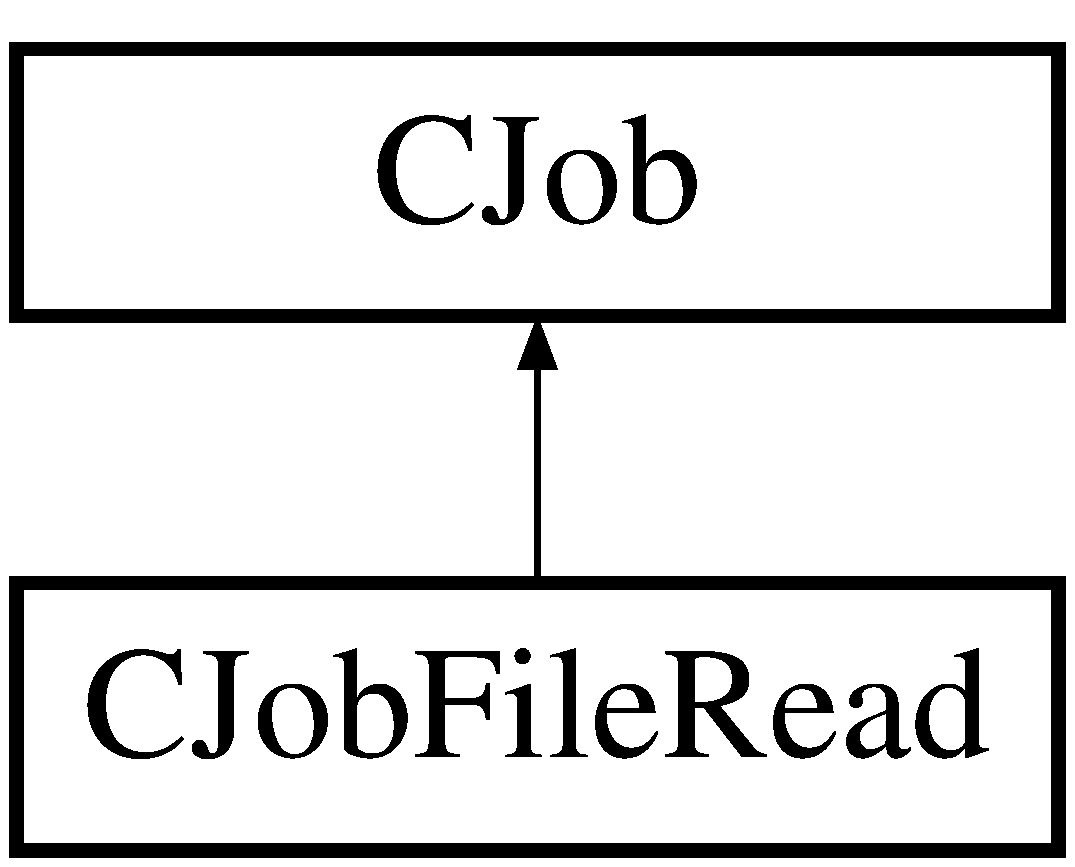
\includegraphics[height=2.000000cm]{class_c_job_file_read}
\end{center}
\end{figure}
\subsection*{公開メンバ関数}
\begin{DoxyCompactItemize}
\item 
\hyperlink{class_c_job_file_read_ad33f2de37cac4b1623e7173ce834323d}{C\+Job\+File\+Read} (\hyperlink{class_c_file_reader}{C\+File\+Reader} $\ast$\+\_\+pc\+Reader)
\begin{DoxyCompactList}\small\item\em コンストラクタ。 \end{DoxyCompactList}\item 
virtual \hyperlink{class_c_job_file_read_aa892176c47cc004a262d64e9a2c71f26}{$\sim$\+C\+Job\+File\+Read} ()
\begin{DoxyCompactList}\small\item\em デストラクタ。 \end{DoxyCompactList}\item 
virtual void \hyperlink{class_c_job_file_read_a0a4d39098eb64debd74d4e2edfac00b9}{Run} () override
\begin{DoxyCompactList}\small\item\em ワーカースレッドで行う処理。 \end{DoxyCompactList}\item 
\hyperlink{class_c_file_reader}{C\+File\+Reader} $\ast$ \hyperlink{class_c_job_file_read_a6c9fc153abd3d4b9888a57d3ba3727a7}{Get\+File\+Reader} () const 
\begin{DoxyCompactList}\small\item\em ファイルリーダーを取得。 \end{DoxyCompactList}\end{DoxyCompactItemize}
\subsection*{非公開変数類}
\begin{DoxyCompactItemize}
\item 
\hyperlink{class_c_file_reader}{C\+File\+Reader} $\ast$ \hyperlink{class_c_job_file_read_a2951a4985790966c91eba8b22e26296a}{m\+\_\+pc\+Reader}
\end{DoxyCompactItemize}


\subsection{構築子と解体子}
\hypertarget{class_c_job_file_read_ad33f2de37cac4b1623e7173ce834323d}{}\index{C\+Job\+File\+Read@{C\+Job\+File\+Read}!C\+Job\+File\+Read@{C\+Job\+File\+Read}}
\index{C\+Job\+File\+Read@{C\+Job\+File\+Read}!C\+Job\+File\+Read@{C\+Job\+File\+Read}}
\subsubsection[{C\+Job\+File\+Read(\+C\+File\+Reader $\ast$\+\_\+pc\+Reader)}]{\setlength{\rightskip}{0pt plus 5cm}C\+Job\+File\+Read\+::\+C\+Job\+File\+Read (
\begin{DoxyParamCaption}
\item[{{\bf C\+File\+Reader} $\ast$}]{\+\_\+pc\+Reader}
\end{DoxyParamCaption}
)}\label{class_c_job_file_read_ad33f2de37cac4b1623e7173ce834323d}


コンストラクタ。 


\begin{DoxyParams}[1]{引数}
\mbox{\tt in}  & {\em \+\_\+pc\+Reader} & \+: ファイル読み込みクラス。 \\
\hline
\end{DoxyParams}
\hypertarget{class_c_job_file_read_aa892176c47cc004a262d64e9a2c71f26}{}\index{C\+Job\+File\+Read@{C\+Job\+File\+Read}!````~C\+Job\+File\+Read@{$\sim$\+C\+Job\+File\+Read}}
\index{````~C\+Job\+File\+Read@{$\sim$\+C\+Job\+File\+Read}!C\+Job\+File\+Read@{C\+Job\+File\+Read}}
\subsubsection[{$\sim$\+C\+Job\+File\+Read()}]{\setlength{\rightskip}{0pt plus 5cm}virtual C\+Job\+File\+Read\+::$\sim$\+C\+Job\+File\+Read (
\begin{DoxyParamCaption}
{}
\end{DoxyParamCaption}
)\hspace{0.3cm}{\ttfamily [inline]}, {\ttfamily [virtual]}}\label{class_c_job_file_read_aa892176c47cc004a262d64e9a2c71f26}


デストラクタ。 



\subsection{関数詳解}
\hypertarget{class_c_job_file_read_a6c9fc153abd3d4b9888a57d3ba3727a7}{}\index{C\+Job\+File\+Read@{C\+Job\+File\+Read}!Get\+File\+Reader@{Get\+File\+Reader}}
\index{Get\+File\+Reader@{Get\+File\+Reader}!C\+Job\+File\+Read@{C\+Job\+File\+Read}}
\subsubsection[{Get\+File\+Reader() const }]{\setlength{\rightskip}{0pt plus 5cm}{\bf C\+File\+Reader}$\ast$ C\+Job\+File\+Read\+::\+Get\+File\+Reader (
\begin{DoxyParamCaption}
{}
\end{DoxyParamCaption}
) const\hspace{0.3cm}{\ttfamily [inline]}}\label{class_c_job_file_read_a6c9fc153abd3d4b9888a57d3ba3727a7}


ファイルリーダーを取得。 

\hypertarget{class_c_job_file_read_a0a4d39098eb64debd74d4e2edfac00b9}{}\index{C\+Job\+File\+Read@{C\+Job\+File\+Read}!Run@{Run}}
\index{Run@{Run}!C\+Job\+File\+Read@{C\+Job\+File\+Read}}
\subsubsection[{Run() override}]{\setlength{\rightskip}{0pt plus 5cm}void C\+Job\+File\+Read\+::\+Run (
\begin{DoxyParamCaption}
{}
\end{DoxyParamCaption}
)\hspace{0.3cm}{\ttfamily [override]}, {\ttfamily [virtual]}}\label{class_c_job_file_read_a0a4d39098eb64debd74d4e2edfac00b9}


ワーカースレッドで行う処理。 



\hyperlink{class_c_job_af5b3f6138549671f6728bae1113777fe}{C\+Job}を再実装しています。



\subsection{メンバ詳解}
\hypertarget{class_c_job_file_read_a2951a4985790966c91eba8b22e26296a}{}\index{C\+Job\+File\+Read@{C\+Job\+File\+Read}!m\+\_\+pc\+Reader@{m\+\_\+pc\+Reader}}
\index{m\+\_\+pc\+Reader@{m\+\_\+pc\+Reader}!C\+Job\+File\+Read@{C\+Job\+File\+Read}}
\subsubsection[{m\+\_\+pc\+Reader}]{\setlength{\rightskip}{0pt plus 5cm}{\bf C\+File\+Reader}$\ast$ C\+Job\+File\+Read\+::m\+\_\+pc\+Reader\hspace{0.3cm}{\ttfamily [private]}}\label{class_c_job_file_read_a2951a4985790966c91eba8b22e26296a}


このクラス詳解は次のファイルから抽出されました\+:\begin{DoxyCompactItemize}
\item 
D\+:/\+Project/\+Game/\+Lib/\+File/\hyperlink{_job_file_read_8h}{Job\+File\+Read.\+h}\item 
D\+:/\+Project/\+Game/\+Lib/\+File/\hyperlink{_job_file_read_8cpp}{Job\+File\+Read.\+cpp}\end{DoxyCompactItemize}

\hypertarget{class_c_main_loop_thread}{}\section{C\+Main\+Loop\+Thread クラス}
\label{class_c_main_loop_thread}\index{C\+Main\+Loop\+Thread@{C\+Main\+Loop\+Thread}}


{\ttfamily \#include $<$Main\+Loop\+Thread.\+h$>$}

C\+Main\+Loop\+Thread の継承関係図\begin{figure}[H]
\begin{center}
\leavevmode
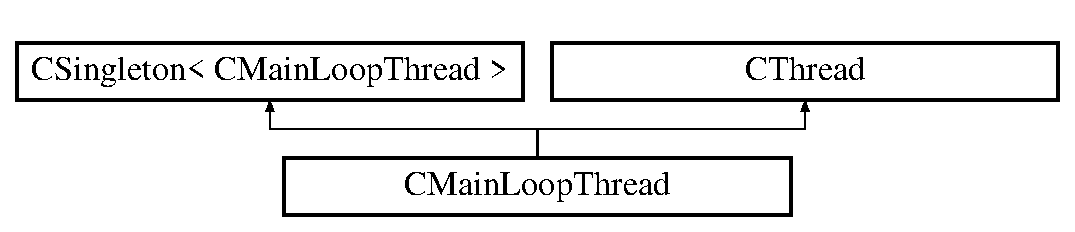
\includegraphics[height=2.000000cm]{class_c_main_loop_thread}
\end{center}
\end{figure}
\subsection*{クラス}
\begin{DoxyCompactItemize}
\item 
struct \hyperlink{struct_c_main_loop_thread_1_1_st_init_param}{St\+Init\+Param}
\begin{DoxyCompactList}\small\item\em 初期化用パラメータ。 \end{DoxyCompactList}\end{DoxyCompactItemize}
\subsection*{公開メンバ関数}
\begin{DoxyCompactItemize}
\item 
virtual \hyperlink{class_c_main_loop_thread_a8f0e8741ac849daa6d0d7ef5a8e01dc0}{$\sim$\+C\+Main\+Loop\+Thread} ()
\begin{DoxyCompactList}\small\item\em デストラクタ。 \end{DoxyCompactList}\item 
void \hyperlink{class_c_main_loop_thread_a69fc8cd33bcabd841a7c73bdd6b2d80d}{Init} (const \hyperlink{struct_c_main_loop_thread_1_1_st_init_param}{St\+Init\+Param} \&\+\_\+rst\+Param)
\begin{DoxyCompactList}\small\item\em 初期化。 \end{DoxyCompactList}\item 
virtual void \hyperlink{class_c_main_loop_thread_a1c3387e62037679993c269d0a3d8daf4}{Thread\+Callback} () override
\begin{DoxyCompactList}\small\item\em スレッドで実行される関数。 \end{DoxyCompactList}\item 
void \hyperlink{class_c_main_loop_thread_a2dc58ab2dd1d0672d7cc3b19ec18f12d}{Main\+Loop} ()
\begin{DoxyCompactList}\small\item\em メインループ。 \end{DoxyCompactList}\item 
void \hyperlink{class_c_main_loop_thread_a7b744d3b869bfb14d66858d070804440}{End} ()
\begin{DoxyCompactList}\small\item\em 終了。 \end{DoxyCompactList}\item 
bool \hyperlink{class_c_main_loop_thread_a358679c3ea651efa39bfe6b9d74c4f7c}{Is\+End} () const 
\begin{DoxyCompactList}\small\item\em 終了したか。 \end{DoxyCompactList}\end{DoxyCompactItemize}
\subsection*{非公開メンバ関数}
\begin{DoxyCompactItemize}
\item 
\hyperlink{class_c_main_loop_thread_aa9cb78870f35c784845d511cfdadbc7d}{C\+Main\+Loop\+Thread} ()
\begin{DoxyCompactList}\small\item\em コンストラクタ。 \end{DoxyCompactList}\end{DoxyCompactItemize}
\subsection*{非公開変数類}
\begin{DoxyCompactItemize}
\item 
friend \hyperlink{class_c_main_loop_thread_aeb2658371223fffe810cd295850b3d16}{C\+Singleton$<$ C\+Main\+Loop\+Thread $>$}
\item 
\hyperlink{class_i_render_context}{I\+Render\+Context} $\ast$ \hyperlink{class_c_main_loop_thread_a074b2d55fb78590fffa4732d687c2154}{m\+\_\+pc\+Render\+Context}
\item 
\hyperlink{class_c_sequence_control}{C\+Sequence\+Control} $\ast$ \hyperlink{class_c_main_loop_thread_aad56c0e06d334140719c29eb5da4664c}{m\+\_\+pc\+Sequence\+Control}
\item 
bool \hyperlink{class_c_main_loop_thread_a4bdbf390f6b77f1c9b1c6c803287ce53}{m\+\_\+b\+End}
\end{DoxyCompactItemize}
\subsection*{その他の継承メンバ}


\subsection{構築子と解体子}
\hypertarget{class_c_main_loop_thread_aa9cb78870f35c784845d511cfdadbc7d}{}\index{C\+Main\+Loop\+Thread@{C\+Main\+Loop\+Thread}!C\+Main\+Loop\+Thread@{C\+Main\+Loop\+Thread}}
\index{C\+Main\+Loop\+Thread@{C\+Main\+Loop\+Thread}!C\+Main\+Loop\+Thread@{C\+Main\+Loop\+Thread}}
\subsubsection[{C\+Main\+Loop\+Thread()}]{\setlength{\rightskip}{0pt plus 5cm}C\+Main\+Loop\+Thread\+::\+C\+Main\+Loop\+Thread (
\begin{DoxyParamCaption}
{}
\end{DoxyParamCaption}
)\hspace{0.3cm}{\ttfamily [private]}}\label{class_c_main_loop_thread_aa9cb78870f35c784845d511cfdadbc7d}


コンストラクタ。 

\hypertarget{class_c_main_loop_thread_a8f0e8741ac849daa6d0d7ef5a8e01dc0}{}\index{C\+Main\+Loop\+Thread@{C\+Main\+Loop\+Thread}!````~C\+Main\+Loop\+Thread@{$\sim$\+C\+Main\+Loop\+Thread}}
\index{````~C\+Main\+Loop\+Thread@{$\sim$\+C\+Main\+Loop\+Thread}!C\+Main\+Loop\+Thread@{C\+Main\+Loop\+Thread}}
\subsubsection[{$\sim$\+C\+Main\+Loop\+Thread()}]{\setlength{\rightskip}{0pt plus 5cm}C\+Main\+Loop\+Thread\+::$\sim$\+C\+Main\+Loop\+Thread (
\begin{DoxyParamCaption}
{}
\end{DoxyParamCaption}
)\hspace{0.3cm}{\ttfamily [virtual]}}\label{class_c_main_loop_thread_a8f0e8741ac849daa6d0d7ef5a8e01dc0}


デストラクタ。 



\subsection{関数詳解}
\hypertarget{class_c_main_loop_thread_a7b744d3b869bfb14d66858d070804440}{}\index{C\+Main\+Loop\+Thread@{C\+Main\+Loop\+Thread}!End@{End}}
\index{End@{End}!C\+Main\+Loop\+Thread@{C\+Main\+Loop\+Thread}}
\subsubsection[{End()}]{\setlength{\rightskip}{0pt plus 5cm}void C\+Main\+Loop\+Thread\+::\+End (
\begin{DoxyParamCaption}
{}
\end{DoxyParamCaption}
)\hspace{0.3cm}{\ttfamily [inline]}}\label{class_c_main_loop_thread_a7b744d3b869bfb14d66858d070804440}


終了。 

\hypertarget{class_c_main_loop_thread_a69fc8cd33bcabd841a7c73bdd6b2d80d}{}\index{C\+Main\+Loop\+Thread@{C\+Main\+Loop\+Thread}!Init@{Init}}
\index{Init@{Init}!C\+Main\+Loop\+Thread@{C\+Main\+Loop\+Thread}}
\subsubsection[{Init(const St\+Init\+Param \&\+\_\+rst\+Param)}]{\setlength{\rightskip}{0pt plus 5cm}void C\+Main\+Loop\+Thread\+::\+Init (
\begin{DoxyParamCaption}
\item[{const {\bf St\+Init\+Param} \&}]{\+\_\+rst\+Param}
\end{DoxyParamCaption}
)}\label{class_c_main_loop_thread_a69fc8cd33bcabd841a7c73bdd6b2d80d}


初期化。 


\begin{DoxyParams}[1]{引数}
\mbox{\tt in}  & {\em \+\_\+rst\+Param} & \+: 初期化用パラメータ。 \\
\hline
\end{DoxyParams}
\hypertarget{class_c_main_loop_thread_a358679c3ea651efa39bfe6b9d74c4f7c}{}\index{C\+Main\+Loop\+Thread@{C\+Main\+Loop\+Thread}!Is\+End@{Is\+End}}
\index{Is\+End@{Is\+End}!C\+Main\+Loop\+Thread@{C\+Main\+Loop\+Thread}}
\subsubsection[{Is\+End() const }]{\setlength{\rightskip}{0pt plus 5cm}bool C\+Main\+Loop\+Thread\+::\+Is\+End (
\begin{DoxyParamCaption}
{}
\end{DoxyParamCaption}
) const\hspace{0.3cm}{\ttfamily [inline]}}\label{class_c_main_loop_thread_a358679c3ea651efa39bfe6b9d74c4f7c}


終了したか。 

\hypertarget{class_c_main_loop_thread_a2dc58ab2dd1d0672d7cc3b19ec18f12d}{}\index{C\+Main\+Loop\+Thread@{C\+Main\+Loop\+Thread}!Main\+Loop@{Main\+Loop}}
\index{Main\+Loop@{Main\+Loop}!C\+Main\+Loop\+Thread@{C\+Main\+Loop\+Thread}}
\subsubsection[{Main\+Loop()}]{\setlength{\rightskip}{0pt plus 5cm}void C\+Main\+Loop\+Thread\+::\+Main\+Loop (
\begin{DoxyParamCaption}
{}
\end{DoxyParamCaption}
)}\label{class_c_main_loop_thread_a2dc58ab2dd1d0672d7cc3b19ec18f12d}


メインループ。 

\hypertarget{class_c_main_loop_thread_a1c3387e62037679993c269d0a3d8daf4}{}\index{C\+Main\+Loop\+Thread@{C\+Main\+Loop\+Thread}!Thread\+Callback@{Thread\+Callback}}
\index{Thread\+Callback@{Thread\+Callback}!C\+Main\+Loop\+Thread@{C\+Main\+Loop\+Thread}}
\subsubsection[{Thread\+Callback() override}]{\setlength{\rightskip}{0pt plus 5cm}virtual void C\+Main\+Loop\+Thread\+::\+Thread\+Callback (
\begin{DoxyParamCaption}
{}
\end{DoxyParamCaption}
)\hspace{0.3cm}{\ttfamily [inline]}, {\ttfamily [override]}, {\ttfamily [virtual]}}\label{class_c_main_loop_thread_a1c3387e62037679993c269d0a3d8daf4}


スレッドで実行される関数。 



\hyperlink{class_c_thread_a15c60ba6d652d92c150fda5e10ebb23e}{C\+Thread}を再実装しています。



\subsection{メンバ詳解}
\hypertarget{class_c_main_loop_thread_aeb2658371223fffe810cd295850b3d16}{}\index{C\+Main\+Loop\+Thread@{C\+Main\+Loop\+Thread}!C\+Singleton$<$ C\+Main\+Loop\+Thread $>$@{C\+Singleton$<$ C\+Main\+Loop\+Thread $>$}}
\index{C\+Singleton$<$ C\+Main\+Loop\+Thread $>$@{C\+Singleton$<$ C\+Main\+Loop\+Thread $>$}!C\+Main\+Loop\+Thread@{C\+Main\+Loop\+Thread}}
\subsubsection[{C\+Singleton$<$ C\+Main\+Loop\+Thread $>$}]{\setlength{\rightskip}{0pt plus 5cm}friend {\bf C\+Main\+Loop\+Thread\+::\+C\+Singleton}$<$ {\bf C\+Main\+Loop\+Thread} $>$\hspace{0.3cm}{\ttfamily [private]}}\label{class_c_main_loop_thread_aeb2658371223fffe810cd295850b3d16}
\hypertarget{class_c_main_loop_thread_a4bdbf390f6b77f1c9b1c6c803287ce53}{}\index{C\+Main\+Loop\+Thread@{C\+Main\+Loop\+Thread}!m\+\_\+b\+End@{m\+\_\+b\+End}}
\index{m\+\_\+b\+End@{m\+\_\+b\+End}!C\+Main\+Loop\+Thread@{C\+Main\+Loop\+Thread}}
\subsubsection[{m\+\_\+b\+End}]{\setlength{\rightskip}{0pt plus 5cm}bool C\+Main\+Loop\+Thread\+::m\+\_\+b\+End\hspace{0.3cm}{\ttfamily [private]}}\label{class_c_main_loop_thread_a4bdbf390f6b77f1c9b1c6c803287ce53}
\hypertarget{class_c_main_loop_thread_a074b2d55fb78590fffa4732d687c2154}{}\index{C\+Main\+Loop\+Thread@{C\+Main\+Loop\+Thread}!m\+\_\+pc\+Render\+Context@{m\+\_\+pc\+Render\+Context}}
\index{m\+\_\+pc\+Render\+Context@{m\+\_\+pc\+Render\+Context}!C\+Main\+Loop\+Thread@{C\+Main\+Loop\+Thread}}
\subsubsection[{m\+\_\+pc\+Render\+Context}]{\setlength{\rightskip}{0pt plus 5cm}{\bf I\+Render\+Context}$\ast$ C\+Main\+Loop\+Thread\+::m\+\_\+pc\+Render\+Context\hspace{0.3cm}{\ttfamily [private]}}\label{class_c_main_loop_thread_a074b2d55fb78590fffa4732d687c2154}
\hypertarget{class_c_main_loop_thread_aad56c0e06d334140719c29eb5da4664c}{}\index{C\+Main\+Loop\+Thread@{C\+Main\+Loop\+Thread}!m\+\_\+pc\+Sequence\+Control@{m\+\_\+pc\+Sequence\+Control}}
\index{m\+\_\+pc\+Sequence\+Control@{m\+\_\+pc\+Sequence\+Control}!C\+Main\+Loop\+Thread@{C\+Main\+Loop\+Thread}}
\subsubsection[{m\+\_\+pc\+Sequence\+Control}]{\setlength{\rightskip}{0pt plus 5cm}{\bf C\+Sequence\+Control}$\ast$ C\+Main\+Loop\+Thread\+::m\+\_\+pc\+Sequence\+Control\hspace{0.3cm}{\ttfamily [private]}}\label{class_c_main_loop_thread_aad56c0e06d334140719c29eb5da4664c}


このクラス詳解は次のファイルから抽出されました\+:\begin{DoxyCompactItemize}
\item 
D\+:/\+Project/\+Game/\+Lib/\+Main\+Loop/\hyperlink{_main_loop_thread_8h}{Main\+Loop\+Thread.\+h}\item 
D\+:/\+Project/\+Game/\+Lib/\+Main\+Loop/\hyperlink{_main_loop_thread_8cpp}{Main\+Loop\+Thread.\+cpp}\end{DoxyCompactItemize}

\hypertarget{class_c_mem_allocator}{}\section{C\+Mem\+Allocator クラス}
\label{class_c_mem_allocator}\index{C\+Mem\+Allocator@{C\+Mem\+Allocator}}


{\ttfamily \#include $<$Mem\+Allocator.\+h$>$}

\subsection*{クラス}
\begin{DoxyCompactItemize}
\item 
struct \hyperlink{struct_c_mem_allocator_1_1_st_init_param}{St\+Init\+Param}
\begin{DoxyCompactList}\small\item\em 初期化用パラメータ。 \end{DoxyCompactList}\end{DoxyCompactItemize}
\subsection*{公開型}
\begin{DoxyCompactItemize}
\item 
enum \hyperlink{class_c_mem_allocator_abf840ff9239492607ab3a3b8e0df2066}{En\+Alloc\+Mode} \+: U32 \{ \hyperlink{class_c_mem_allocator_abf840ff9239492607ab3a3b8e0df2066a51de7c871812c0d91929b2fa407db09f}{En\+Alloc\+Mode\+::en\+Forward}, 
\hyperlink{class_c_mem_allocator_abf840ff9239492607ab3a3b8e0df2066a3b7d737dc6a726f089f8d85df120a77f}{En\+Alloc\+Mode\+::en\+Back}
 \}\begin{DoxyCompactList}\small\item\em アロケートモード。 \end{DoxyCompactList}
\end{DoxyCompactItemize}
\subsection*{公開メンバ関数}
\begin{DoxyCompactItemize}
\item 
\hyperlink{class_c_mem_allocator_a89a6785ad0679112693421390834c58a}{C\+Mem\+Allocator} (const \hyperlink{struct_c_mem_allocator_1_1_st_init_param}{St\+Init\+Param} \&\+\_\+rst\+Init\+Param)
\begin{DoxyCompactList}\small\item\em コンストラクタ。 \end{DoxyCompactList}\item 
virtual \hyperlink{class_c_mem_allocator_afcf3bf84876c42ab83cdc2ba10a7dac3}{$\sim$\+C\+Mem\+Allocator} ()
\begin{DoxyCompactList}\small\item\em デストラクタ。 \end{DoxyCompactList}\item 
void $\ast$ \hyperlink{class_c_mem_allocator_a65875035e030185e91391b1ce29eecdd}{Alloc} (U\+Size \+\_\+u\+Size, const S8 $\ast$\+\_\+ps\+File, U32 \+\_\+u\+Line)
\begin{DoxyCompactList}\small\item\em メモリを確保。 \end{DoxyCompactList}\item 
void $\ast$ \hyperlink{class_c_mem_allocator_a776e73bfdd517d758ccfe515298d6716}{Alloc\+Back} (U\+Size \+\_\+u\+Size, const S8 $\ast$\+\_\+ps\+File, U32 \+\_\+u\+Line)
\begin{DoxyCompactList}\small\item\em 最後尾からメモリを確保。 \end{DoxyCompactList}\item 
void $\ast$ \hyperlink{class_c_mem_allocator_a78bd707276d68fc2aa5828dbb86a74df}{Alloc\+From\+Mem\+Block} (\hyperlink{class_c_mem_block}{C\+Mem\+Block} $\ast$\+\_\+pc\+Mem\+Block, U\+Size \+\_\+u\+Size, const S8 $\ast$\+\_\+ps\+File, U32 \+\_\+u\+Line, \hyperlink{class_c_mem_allocator_abf840ff9239492607ab3a3b8e0df2066}{En\+Alloc\+Mode} \+\_\+e\+Mode)
\begin{DoxyCompactList}\small\item\em 指定したメモリブロックからメモリを確保。 \end{DoxyCompactList}\item 
void \hyperlink{class_c_mem_allocator_ac679b89a322afa320a994d8bedec415d}{Free} (void $\ast$\+\_\+p)
\begin{DoxyCompactList}\small\item\em メモリを解放。 \end{DoxyCompactList}\item 
bool \hyperlink{class_c_mem_allocator_ab3c38b86c68cfc86a3e95bb7964efd97}{Is\+Allocated\+Pointer} (void $\ast$\+\_\+p) const 
\begin{DoxyCompactList}\small\item\em このメモリアロケータで確保したポインタか。 \end{DoxyCompactList}\end{DoxyCompactItemize}
\subsection*{静的公開メンバ関数}
\begin{DoxyCompactItemize}
\item 
static void $\ast$ \hyperlink{class_c_mem_allocator_a48c0568fb21eb63978af2137aab23ad6}{operator new} (std\+::size\+\_\+t \+\_\+u\+Size)
\item 
static void \hyperlink{class_c_mem_allocator_af156badb5f8380a0d9ee76afad22c496}{operator delete} (void $\ast$\+\_\+p)
\end{DoxyCompactItemize}
\subsection*{非公開型}
\begin{DoxyCompactItemize}
\item 
enum \hyperlink{class_c_mem_allocator_a780a1a1225569ea2d2a8b7db9f9c7089}{En\+First\+Level} \{ \hyperlink{class_c_mem_allocator_a780a1a1225569ea2d2a8b7db9f9c7089ab914654c48cd4a1779f988840ea2a151}{en\+First\+Level\+\_\+\+Max} = sizeof( U\+Size ) $\ast$ 8
 \}\begin{DoxyCompactList}\small\item\em First\+Level。 \end{DoxyCompactList}
\end{DoxyCompactItemize}
\subsection*{非公開メンバ関数}
\begin{DoxyCompactItemize}
\item 
U\+Size \hyperlink{class_c_mem_allocator_a920fe29d9b0bdaa721eaa20c66abaa2e}{Get\+Block\+Size} (U\+Size \+\_\+u\+Size)
\begin{DoxyCompactList}\small\item\em 要求されたサイズから、実際に確保するブロックサイズを取得。 \end{DoxyCompactList}\item 
void \hyperlink{class_c_mem_allocator_af607e6b68b3b614e769b6e93078a04ca}{Get\+Level} (U32 $\ast$\+\_\+pu\+Out\+First, U32 $\ast$\+\_\+pu\+Out\+Second, U\+Size \+\_\+u\+Block\+Size)
\begin{DoxyCompactList}\small\item\em サイズからレベルを取得。 \end{DoxyCompactList}\item 
void \hyperlink{class_c_mem_allocator_a7a916e62db377590430d6969551cc547}{Set\+Free\+List} (\hyperlink{class_c_mem_block}{C\+Mem\+Block} $\ast$\+\_\+pc\+Mem\+Block)
\begin{DoxyCompactList}\small\item\em Freeリストに領域をセット。 \end{DoxyCompactList}\item 
void \hyperlink{class_c_mem_allocator_a54bea8680421134c27912868508792aa}{Remove\+Free\+List} (\hyperlink{class_c_mem_block}{C\+Mem\+Block} $\ast$\+\_\+pc\+Mem\+Block)
\begin{DoxyCompactList}\small\item\em Freeリストから領域を解除。 \end{DoxyCompactList}\item 
bool \hyperlink{class_c_mem_allocator_a5157e10cc3b426b42f661a6f3c0d8f51}{Search\+Free\+List\+Level} (U32 $\ast$\+\_\+p\+Out\+First\+Level, U32 $\ast$\+\_\+p\+Out\+Second\+Level, U\+Size \+\_\+u\+Block\+Size)
\begin{DoxyCompactList}\small\item\em Freeリストから確保出来る領域のレベルを探す。 \end{DoxyCompactList}\item 
U32 \hyperlink{class_c_mem_allocator_a9f0303603e63a742cc97c82d64fe90d5}{Get\+Free\+List\+Index} (U32 \+\_\+u\+First\+Level, U32 \+\_\+u\+Second\+Level)
\begin{DoxyCompactList}\small\item\em レベルから\+Freeリストのインデックスを取得。 \end{DoxyCompactList}\end{DoxyCompactItemize}
\subsection*{非公開変数類}
\begin{DoxyCompactItemize}
\item 
\hyperlink{struct_c_mem_allocator_1_1_st_init_param}{St\+Init\+Param} \hyperlink{class_c_mem_allocator_a5ae9573631f11b58cb0741dd5d071d4e}{m\+\_\+st\+Init\+Param}
\item 
U8 $\ast$ \hyperlink{class_c_mem_allocator_ad729846ce9ff5ecdac69574604140e39}{m\+\_\+p\+Memory}
\begin{DoxyCompactList}\small\item\em 確保したメモリ。 \end{DoxyCompactList}\item 
\hyperlink{class_c_mem_block}{C\+Mem\+Block} $\ast$ \hyperlink{class_c_mem_allocator_aac2d7de345dbb577fa47907647bb831f}{m\+\_\+p\+End\+Block}
\begin{DoxyCompactList}\small\item\em 終端ブロック。 \end{DoxyCompactList}\item 
\hyperlink{class_c_mem_block}{C\+Mem\+Block} $\ast$$\ast$ \hyperlink{class_c_mem_allocator_a5593b5d4263ee5e0af22458ad8f89f21}{m\+\_\+p\+Free\+Block\+Array}
\begin{DoxyCompactList}\small\item\em 解放済みの領域リスト。 \end{DoxyCompactList}\item 
U64 \hyperlink{class_c_mem_allocator_a9f35f48a378b79fc033b6aa6dcf13b73}{m\+\_\+u\+Is\+Free}
\begin{DoxyCompactList}\small\item\em 解放済みの領域があるか。(1st\+Level) \end{DoxyCompactList}\item 
U32 \hyperlink{class_c_mem_allocator_a6fc0c334bf8f88d108b7f7ca1b87c682}{m\+\_\+u\+Is\+Free\+Array} \mbox{[}\hyperlink{class_c_mem_allocator_a780a1a1225569ea2d2a8b7db9f9c7089ab914654c48cd4a1779f988840ea2a151}{en\+First\+Level\+\_\+\+Max}\mbox{]}
\begin{DoxyCompactList}\small\item\em 解放済みの領域があるか。(2nd\+Level) \end{DoxyCompactList}\item 
\hyperlink{class_c_critical_section}{C\+Critical\+Section} \hyperlink{class_c_mem_allocator_ac777d3d046eab9d58e8749a68a6bf36c}{m\+\_\+c\+Critical\+Section}
\begin{DoxyCompactList}\small\item\em クリティカルセクション。 \end{DoxyCompactList}\end{DoxyCompactItemize}


\subsection{列挙型メンバ詳解}
\hypertarget{class_c_mem_allocator_abf840ff9239492607ab3a3b8e0df2066}{}\index{C\+Mem\+Allocator@{C\+Mem\+Allocator}!En\+Alloc\+Mode@{En\+Alloc\+Mode}}
\index{En\+Alloc\+Mode@{En\+Alloc\+Mode}!C\+Mem\+Allocator@{C\+Mem\+Allocator}}
\subsubsection[{En\+Alloc\+Mode}]{\setlength{\rightskip}{0pt plus 5cm}enum {\bf C\+Mem\+Allocator\+::\+En\+Alloc\+Mode} \+: U32\hspace{0.3cm}{\ttfamily [strong]}}\label{class_c_mem_allocator_abf840ff9239492607ab3a3b8e0df2066}


アロケートモード。 

\begin{Desc}
\item[列挙値]\par
\begin{description}
\index{en\+Forward@{en\+Forward}!C\+Mem\+Allocator@{C\+Mem\+Allocator}}\index{C\+Mem\+Allocator@{C\+Mem\+Allocator}!en\+Forward@{en\+Forward}}\item[{\em 
\hypertarget{class_c_mem_allocator_abf840ff9239492607ab3a3b8e0df2066a51de7c871812c0d91929b2fa407db09f}{}en\+Forward\label{class_c_mem_allocator_abf840ff9239492607ab3a3b8e0df2066a51de7c871812c0d91929b2fa407db09f}
}]\index{en\+Back@{en\+Back}!C\+Mem\+Allocator@{C\+Mem\+Allocator}}\index{C\+Mem\+Allocator@{C\+Mem\+Allocator}!en\+Back@{en\+Back}}\item[{\em 
\hypertarget{class_c_mem_allocator_abf840ff9239492607ab3a3b8e0df2066a3b7d737dc6a726f089f8d85df120a77f}{}en\+Back\label{class_c_mem_allocator_abf840ff9239492607ab3a3b8e0df2066a3b7d737dc6a726f089f8d85df120a77f}
}]\end{description}
\end{Desc}
\hypertarget{class_c_mem_allocator_a780a1a1225569ea2d2a8b7db9f9c7089}{}\index{C\+Mem\+Allocator@{C\+Mem\+Allocator}!En\+First\+Level@{En\+First\+Level}}
\index{En\+First\+Level@{En\+First\+Level}!C\+Mem\+Allocator@{C\+Mem\+Allocator}}
\subsubsection[{En\+First\+Level}]{\setlength{\rightskip}{0pt plus 5cm}enum {\bf C\+Mem\+Allocator\+::\+En\+First\+Level}\hspace{0.3cm}{\ttfamily [private]}}\label{class_c_mem_allocator_a780a1a1225569ea2d2a8b7db9f9c7089}


First\+Level。 

\begin{Desc}
\item[列挙値]\par
\begin{description}
\index{en\+First\+Level\+\_\+\+Max@{en\+First\+Level\+\_\+\+Max}!C\+Mem\+Allocator@{C\+Mem\+Allocator}}\index{C\+Mem\+Allocator@{C\+Mem\+Allocator}!en\+First\+Level\+\_\+\+Max@{en\+First\+Level\+\_\+\+Max}}\item[{\em 
\hypertarget{class_c_mem_allocator_a780a1a1225569ea2d2a8b7db9f9c7089ab914654c48cd4a1779f988840ea2a151}{}en\+First\+Level\+\_\+\+Max\label{class_c_mem_allocator_a780a1a1225569ea2d2a8b7db9f9c7089ab914654c48cd4a1779f988840ea2a151}
}]\end{description}
\end{Desc}


\subsection{構築子と解体子}
\hypertarget{class_c_mem_allocator_a89a6785ad0679112693421390834c58a}{}\index{C\+Mem\+Allocator@{C\+Mem\+Allocator}!C\+Mem\+Allocator@{C\+Mem\+Allocator}}
\index{C\+Mem\+Allocator@{C\+Mem\+Allocator}!C\+Mem\+Allocator@{C\+Mem\+Allocator}}
\subsubsection[{C\+Mem\+Allocator(const St\+Init\+Param \&\+\_\+rst\+Init\+Param)}]{\setlength{\rightskip}{0pt plus 5cm}C\+Mem\+Allocator\+::\+C\+Mem\+Allocator (
\begin{DoxyParamCaption}
\item[{const {\bf St\+Init\+Param} \&}]{\+\_\+rst\+Init\+Param}
\end{DoxyParamCaption}
)}\label{class_c_mem_allocator_a89a6785ad0679112693421390834c58a}


コンストラクタ。 


\begin{DoxyParams}[1]{引数}
\mbox{\tt in}  & {\em \+\_\+rst\+Init\+Param} & \+: 初期化用パラメータ \\
\hline
\end{DoxyParams}
\hypertarget{class_c_mem_allocator_afcf3bf84876c42ab83cdc2ba10a7dac3}{}\index{C\+Mem\+Allocator@{C\+Mem\+Allocator}!````~C\+Mem\+Allocator@{$\sim$\+C\+Mem\+Allocator}}
\index{````~C\+Mem\+Allocator@{$\sim$\+C\+Mem\+Allocator}!C\+Mem\+Allocator@{C\+Mem\+Allocator}}
\subsubsection[{$\sim$\+C\+Mem\+Allocator()}]{\setlength{\rightskip}{0pt plus 5cm}C\+Mem\+Allocator\+::$\sim$\+C\+Mem\+Allocator (
\begin{DoxyParamCaption}
{}
\end{DoxyParamCaption}
)\hspace{0.3cm}{\ttfamily [virtual]}}\label{class_c_mem_allocator_afcf3bf84876c42ab83cdc2ba10a7dac3}


デストラクタ。 



\subsection{関数詳解}
\hypertarget{class_c_mem_allocator_a65875035e030185e91391b1ce29eecdd}{}\index{C\+Mem\+Allocator@{C\+Mem\+Allocator}!Alloc@{Alloc}}
\index{Alloc@{Alloc}!C\+Mem\+Allocator@{C\+Mem\+Allocator}}
\subsubsection[{Alloc(\+U\+Size \+\_\+u\+Size, const S8 $\ast$\+\_\+ps\+File, U32 \+\_\+u\+Line)}]{\setlength{\rightskip}{0pt plus 5cm}void $\ast$ C\+Mem\+Allocator\+::\+Alloc (
\begin{DoxyParamCaption}
\item[{U\+Size}]{\+\_\+u\+Size, }
\item[{const S8 $\ast$}]{\+\_\+ps\+File, }
\item[{U32}]{\+\_\+u\+Line}
\end{DoxyParamCaption}
)}\label{class_c_mem_allocator_a65875035e030185e91391b1ce29eecdd}


メモリを確保。 


\begin{DoxyParams}[1]{引数}
\mbox{\tt in}  & {\em \+\_\+u\+Size} & \+: 確保するサイズ。 \\
\hline
\mbox{\tt in}  & {\em \+\_\+ps\+File} & \+: 呼び出し元のファイル名。 \\
\hline
\mbox{\tt in}  & {\em \+\_\+u\+Line} & \+: 呼び出し元行数。 \\
\hline
\end{DoxyParams}
\begin{DoxyReturn}{戻り値}
\+: 確保したメモリへのポインタ。 
\end{DoxyReturn}
\hypertarget{class_c_mem_allocator_a776e73bfdd517d758ccfe515298d6716}{}\index{C\+Mem\+Allocator@{C\+Mem\+Allocator}!Alloc\+Back@{Alloc\+Back}}
\index{Alloc\+Back@{Alloc\+Back}!C\+Mem\+Allocator@{C\+Mem\+Allocator}}
\subsubsection[{Alloc\+Back(\+U\+Size \+\_\+u\+Size, const S8 $\ast$\+\_\+ps\+File, U32 \+\_\+u\+Line)}]{\setlength{\rightskip}{0pt plus 5cm}void $\ast$ C\+Mem\+Allocator\+::\+Alloc\+Back (
\begin{DoxyParamCaption}
\item[{U\+Size}]{\+\_\+u\+Size, }
\item[{const S8 $\ast$}]{\+\_\+ps\+File, }
\item[{U32}]{\+\_\+u\+Line}
\end{DoxyParamCaption}
)}\label{class_c_mem_allocator_a776e73bfdd517d758ccfe515298d6716}


最後尾からメモリを確保。 


\begin{DoxyParams}[1]{引数}
\mbox{\tt in}  & {\em \+\_\+u\+Size} & \+: 確保するサイズ。 \\
\hline
\mbox{\tt in}  & {\em \+\_\+ps\+File} & \+: 呼び出し元のファイル名。 \\
\hline
\mbox{\tt in}  & {\em \+\_\+u\+Line} & \+: 呼び出し元行数。 \\
\hline
\end{DoxyParams}
\begin{DoxyReturn}{戻り値}
\+: 確保したメモリへのポインタ。 
\end{DoxyReturn}
\hypertarget{class_c_mem_allocator_a78bd707276d68fc2aa5828dbb86a74df}{}\index{C\+Mem\+Allocator@{C\+Mem\+Allocator}!Alloc\+From\+Mem\+Block@{Alloc\+From\+Mem\+Block}}
\index{Alloc\+From\+Mem\+Block@{Alloc\+From\+Mem\+Block}!C\+Mem\+Allocator@{C\+Mem\+Allocator}}
\subsubsection[{Alloc\+From\+Mem\+Block(\+C\+Mem\+Block $\ast$\+\_\+pc\+Mem\+Block, U\+Size \+\_\+u\+Size, const S8 $\ast$\+\_\+ps\+File, U32 \+\_\+u\+Line, En\+Alloc\+Mode \+\_\+e\+Mode)}]{\setlength{\rightskip}{0pt plus 5cm}void $\ast$ C\+Mem\+Allocator\+::\+Alloc\+From\+Mem\+Block (
\begin{DoxyParamCaption}
\item[{{\bf C\+Mem\+Block} $\ast$}]{\+\_\+pc\+Mem\+Block, }
\item[{U\+Size}]{\+\_\+u\+Size, }
\item[{const S8 $\ast$}]{\+\_\+ps\+File, }
\item[{U32}]{\+\_\+u\+Line, }
\item[{{\bf En\+Alloc\+Mode}}]{\+\_\+e\+Mode}
\end{DoxyParamCaption}
)}\label{class_c_mem_allocator_a78bd707276d68fc2aa5828dbb86a74df}


指定したメモリブロックからメモリを確保。 


\begin{DoxyParams}[1]{引数}
\mbox{\tt in}  & {\em \+\_\+pc\+Mem\+Block} & ; メモリブロック。 \\
\hline
\mbox{\tt in}  & {\em \+\_\+u\+Size} & \+: 確保するサイズ。 \\
\hline
\mbox{\tt in}  & {\em \+\_\+ps\+File} & \+: 呼び出し元のファイル名。 \\
\hline
\mbox{\tt in}  & {\em \+\_\+u\+Line} & \+: 呼び出し元行数。 \\
\hline
\mbox{\tt in}  & {\em \+\_\+e\+Mode} & \+: アロケートモード。 \\
\hline
\end{DoxyParams}
\begin{DoxyReturn}{戻り値}
\+: 確保したメモリへのポインタ。 
\end{DoxyReturn}
\hypertarget{class_c_mem_allocator_ac679b89a322afa320a994d8bedec415d}{}\index{C\+Mem\+Allocator@{C\+Mem\+Allocator}!Free@{Free}}
\index{Free@{Free}!C\+Mem\+Allocator@{C\+Mem\+Allocator}}
\subsubsection[{Free(void $\ast$\+\_\+p)}]{\setlength{\rightskip}{0pt plus 5cm}void C\+Mem\+Allocator\+::\+Free (
\begin{DoxyParamCaption}
\item[{void $\ast$}]{\+\_\+p}
\end{DoxyParamCaption}
)}\label{class_c_mem_allocator_ac679b89a322afa320a994d8bedec415d}


メモリを解放。 

brief メモリを解放。 \hypertarget{class_c_mem_allocator_a920fe29d9b0bdaa721eaa20c66abaa2e}{}\index{C\+Mem\+Allocator@{C\+Mem\+Allocator}!Get\+Block\+Size@{Get\+Block\+Size}}
\index{Get\+Block\+Size@{Get\+Block\+Size}!C\+Mem\+Allocator@{C\+Mem\+Allocator}}
\subsubsection[{Get\+Block\+Size(\+U\+Size \+\_\+u\+Size)}]{\setlength{\rightskip}{0pt plus 5cm}U\+Size C\+Mem\+Allocator\+::\+Get\+Block\+Size (
\begin{DoxyParamCaption}
\item[{U\+Size}]{\+\_\+u\+Size}
\end{DoxyParamCaption}
)\hspace{0.3cm}{\ttfamily [inline]}, {\ttfamily [private]}}\label{class_c_mem_allocator_a920fe29d9b0bdaa721eaa20c66abaa2e}


要求されたサイズから、実際に確保するブロックサイズを取得。 

\hypertarget{class_c_mem_allocator_a9f0303603e63a742cc97c82d64fe90d5}{}\index{C\+Mem\+Allocator@{C\+Mem\+Allocator}!Get\+Free\+List\+Index@{Get\+Free\+List\+Index}}
\index{Get\+Free\+List\+Index@{Get\+Free\+List\+Index}!C\+Mem\+Allocator@{C\+Mem\+Allocator}}
\subsubsection[{Get\+Free\+List\+Index(\+U32 \+\_\+u\+First\+Level, U32 \+\_\+u\+Second\+Level)}]{\setlength{\rightskip}{0pt plus 5cm}U32 C\+Mem\+Allocator\+::\+Get\+Free\+List\+Index (
\begin{DoxyParamCaption}
\item[{U32}]{\+\_\+u\+First\+Level, }
\item[{U32}]{\+\_\+u\+Second\+Level}
\end{DoxyParamCaption}
)\hspace{0.3cm}{\ttfamily [private]}}\label{class_c_mem_allocator_a9f0303603e63a742cc97c82d64fe90d5}


レベルから\+Freeリストのインデックスを取得。 


\begin{DoxyParams}[1]{引数}
\mbox{\tt in}  & {\em \+\_\+u\+First\+Level} & \\
\hline
\mbox{\tt in}  & {\em \+\_\+u\+Second\+Level} & \\
\hline
\end{DoxyParams}

\begin{DoxyRetVals}{戻り値}
{\em インデックス値} & \\
\hline
\end{DoxyRetVals}
\hypertarget{class_c_mem_allocator_af607e6b68b3b614e769b6e93078a04ca}{}\index{C\+Mem\+Allocator@{C\+Mem\+Allocator}!Get\+Level@{Get\+Level}}
\index{Get\+Level@{Get\+Level}!C\+Mem\+Allocator@{C\+Mem\+Allocator}}
\subsubsection[{Get\+Level(\+U32 $\ast$\+\_\+pu\+Out\+First, U32 $\ast$\+\_\+pu\+Out\+Second, U\+Size \+\_\+u\+Block\+Size)}]{\setlength{\rightskip}{0pt plus 5cm}void C\+Mem\+Allocator\+::\+Get\+Level (
\begin{DoxyParamCaption}
\item[{U32 $\ast$}]{\+\_\+pu\+Out\+First, }
\item[{U32 $\ast$}]{\+\_\+pu\+Out\+Second, }
\item[{U\+Size}]{\+\_\+u\+Block\+Size}
\end{DoxyParamCaption}
)\hspace{0.3cm}{\ttfamily [private]}}\label{class_c_mem_allocator_af607e6b68b3b614e769b6e93078a04ca}


サイズからレベルを取得。 


\begin{DoxyParams}[1]{引数}
\mbox{\tt out}  & {\em \+\_\+pu\+Out\+First} & \+: F\+L\+I格納先。 \\
\hline
\mbox{\tt out}  & {\em \+\_\+pu\+Out\+Second} & \+: S\+L\+I格納先。 \\
\hline
\mbox{\tt in}  & {\em \+\_\+u\+Block\+Size} & \+: ブロックサイズ。 \\
\hline
\end{DoxyParams}
\hypertarget{class_c_mem_allocator_ab3c38b86c68cfc86a3e95bb7964efd97}{}\index{C\+Mem\+Allocator@{C\+Mem\+Allocator}!Is\+Allocated\+Pointer@{Is\+Allocated\+Pointer}}
\index{Is\+Allocated\+Pointer@{Is\+Allocated\+Pointer}!C\+Mem\+Allocator@{C\+Mem\+Allocator}}
\subsubsection[{Is\+Allocated\+Pointer(void $\ast$\+\_\+p) const }]{\setlength{\rightskip}{0pt plus 5cm}bool C\+Mem\+Allocator\+::\+Is\+Allocated\+Pointer (
\begin{DoxyParamCaption}
\item[{void $\ast$}]{\+\_\+p}
\end{DoxyParamCaption}
) const}\label{class_c_mem_allocator_ab3c38b86c68cfc86a3e95bb7964efd97}


このメモリアロケータで確保したポインタか。 


\begin{DoxyParams}[1]{引数}
\mbox{\tt in}  & {\em \+\_\+p} & \+: チェックするポインタ。 \\
\hline
\end{DoxyParams}

\begin{DoxyRetVals}{戻り値}
{\em } & \\
\hline
\end{DoxyRetVals}
\hypertarget{class_c_mem_allocator_af156badb5f8380a0d9ee76afad22c496}{}\index{C\+Mem\+Allocator@{C\+Mem\+Allocator}!operator delete@{operator delete}}
\index{operator delete@{operator delete}!C\+Mem\+Allocator@{C\+Mem\+Allocator}}
\subsubsection[{operator delete(void $\ast$\+\_\+p)}]{\setlength{\rightskip}{0pt plus 5cm}static void C\+Mem\+Allocator\+::operator delete (
\begin{DoxyParamCaption}
\item[{void $\ast$}]{\+\_\+p}
\end{DoxyParamCaption}
)\hspace{0.3cm}{\ttfamily [inline]}, {\ttfamily [static]}}\label{class_c_mem_allocator_af156badb5f8380a0d9ee76afad22c496}
\hypertarget{class_c_mem_allocator_a48c0568fb21eb63978af2137aab23ad6}{}\index{C\+Mem\+Allocator@{C\+Mem\+Allocator}!operator new@{operator new}}
\index{operator new@{operator new}!C\+Mem\+Allocator@{C\+Mem\+Allocator}}
\subsubsection[{operator new(std\+::size\+\_\+t \+\_\+u\+Size)}]{\setlength{\rightskip}{0pt plus 5cm}static void$\ast$ C\+Mem\+Allocator\+::operator new (
\begin{DoxyParamCaption}
\item[{std\+::size\+\_\+t}]{\+\_\+u\+Size}
\end{DoxyParamCaption}
)\hspace{0.3cm}{\ttfamily [inline]}, {\ttfamily [static]}}\label{class_c_mem_allocator_a48c0568fb21eb63978af2137aab23ad6}
\hypertarget{class_c_mem_allocator_a54bea8680421134c27912868508792aa}{}\index{C\+Mem\+Allocator@{C\+Mem\+Allocator}!Remove\+Free\+List@{Remove\+Free\+List}}
\index{Remove\+Free\+List@{Remove\+Free\+List}!C\+Mem\+Allocator@{C\+Mem\+Allocator}}
\subsubsection[{Remove\+Free\+List(\+C\+Mem\+Block $\ast$\+\_\+pc\+Mem\+Block)}]{\setlength{\rightskip}{0pt plus 5cm}void C\+Mem\+Allocator\+::\+Remove\+Free\+List (
\begin{DoxyParamCaption}
\item[{{\bf C\+Mem\+Block} $\ast$}]{\+\_\+pc\+Mem\+Block}
\end{DoxyParamCaption}
)\hspace{0.3cm}{\ttfamily [private]}}\label{class_c_mem_allocator_a54bea8680421134c27912868508792aa}


Freeリストから領域を解除。 


\begin{DoxyParams}[1]{引数}
\mbox{\tt in}  & {\em \+\_\+pc\+Mem\+Block} & \+: 解除するブロック。 \\
\hline
\end{DoxyParams}
\hypertarget{class_c_mem_allocator_a5157e10cc3b426b42f661a6f3c0d8f51}{}\index{C\+Mem\+Allocator@{C\+Mem\+Allocator}!Search\+Free\+List\+Level@{Search\+Free\+List\+Level}}
\index{Search\+Free\+List\+Level@{Search\+Free\+List\+Level}!C\+Mem\+Allocator@{C\+Mem\+Allocator}}
\subsubsection[{Search\+Free\+List\+Level(\+U32 $\ast$\+\_\+p\+Out\+First\+Level, U32 $\ast$\+\_\+p\+Out\+Second\+Level, U\+Size \+\_\+u\+Block\+Size)}]{\setlength{\rightskip}{0pt plus 5cm}bool C\+Mem\+Allocator\+::\+Search\+Free\+List\+Level (
\begin{DoxyParamCaption}
\item[{U32 $\ast$}]{\+\_\+p\+Out\+First\+Level, }
\item[{U32 $\ast$}]{\+\_\+p\+Out\+Second\+Level, }
\item[{U\+Size}]{\+\_\+u\+Block\+Size}
\end{DoxyParamCaption}
)\hspace{0.3cm}{\ttfamily [private]}}\label{class_c_mem_allocator_a5157e10cc3b426b42f661a6f3c0d8f51}


Freeリストから確保出来る領域のレベルを探す。 


\begin{DoxyParams}[1]{引数}
\mbox{\tt out}  & {\em \+\_\+p\+Out\+First\+Level} & \+: 1st\+Levelの格納先。 \\
\hline
\mbox{\tt out}  & {\em \+\_\+p\+Out\+Second\+Level} & \+: 2nd\+Levelの格納先。 \\
\hline
\mbox{\tt in}  & {\em \+\_\+u\+Block\+Size} & \+: ブロックサイズ。 \\
\hline
\end{DoxyParams}
\hypertarget{class_c_mem_allocator_a7a916e62db377590430d6969551cc547}{}\index{C\+Mem\+Allocator@{C\+Mem\+Allocator}!Set\+Free\+List@{Set\+Free\+List}}
\index{Set\+Free\+List@{Set\+Free\+List}!C\+Mem\+Allocator@{C\+Mem\+Allocator}}
\subsubsection[{Set\+Free\+List(\+C\+Mem\+Block $\ast$\+\_\+pc\+Mem\+Block)}]{\setlength{\rightskip}{0pt plus 5cm}void C\+Mem\+Allocator\+::\+Set\+Free\+List (
\begin{DoxyParamCaption}
\item[{{\bf C\+Mem\+Block} $\ast$}]{\+\_\+pc\+Mem\+Block}
\end{DoxyParamCaption}
)\hspace{0.3cm}{\ttfamily [private]}}\label{class_c_mem_allocator_a7a916e62db377590430d6969551cc547}


Freeリストに領域をセット。 


\begin{DoxyParams}[1]{引数}
\mbox{\tt in}  & {\em \+\_\+pc\+Mem\+Block} & \+: セットするブロック。 \\
\hline
\end{DoxyParams}


\subsection{メンバ詳解}
\hypertarget{class_c_mem_allocator_ac777d3d046eab9d58e8749a68a6bf36c}{}\index{C\+Mem\+Allocator@{C\+Mem\+Allocator}!m\+\_\+c\+Critical\+Section@{m\+\_\+c\+Critical\+Section}}
\index{m\+\_\+c\+Critical\+Section@{m\+\_\+c\+Critical\+Section}!C\+Mem\+Allocator@{C\+Mem\+Allocator}}
\subsubsection[{m\+\_\+c\+Critical\+Section}]{\setlength{\rightskip}{0pt plus 5cm}{\bf C\+Critical\+Section} C\+Mem\+Allocator\+::m\+\_\+c\+Critical\+Section\hspace{0.3cm}{\ttfamily [private]}}\label{class_c_mem_allocator_ac777d3d046eab9d58e8749a68a6bf36c}


クリティカルセクション。 

\hypertarget{class_c_mem_allocator_aac2d7de345dbb577fa47907647bb831f}{}\index{C\+Mem\+Allocator@{C\+Mem\+Allocator}!m\+\_\+p\+End\+Block@{m\+\_\+p\+End\+Block}}
\index{m\+\_\+p\+End\+Block@{m\+\_\+p\+End\+Block}!C\+Mem\+Allocator@{C\+Mem\+Allocator}}
\subsubsection[{m\+\_\+p\+End\+Block}]{\setlength{\rightskip}{0pt plus 5cm}{\bf C\+Mem\+Block}$\ast$ C\+Mem\+Allocator\+::m\+\_\+p\+End\+Block\hspace{0.3cm}{\ttfamily [private]}}\label{class_c_mem_allocator_aac2d7de345dbb577fa47907647bb831f}


終端ブロック。 

\hypertarget{class_c_mem_allocator_a5593b5d4263ee5e0af22458ad8f89f21}{}\index{C\+Mem\+Allocator@{C\+Mem\+Allocator}!m\+\_\+p\+Free\+Block\+Array@{m\+\_\+p\+Free\+Block\+Array}}
\index{m\+\_\+p\+Free\+Block\+Array@{m\+\_\+p\+Free\+Block\+Array}!C\+Mem\+Allocator@{C\+Mem\+Allocator}}
\subsubsection[{m\+\_\+p\+Free\+Block\+Array}]{\setlength{\rightskip}{0pt plus 5cm}{\bf C\+Mem\+Block}$\ast$$\ast$ C\+Mem\+Allocator\+::m\+\_\+p\+Free\+Block\+Array\hspace{0.3cm}{\ttfamily [private]}}\label{class_c_mem_allocator_a5593b5d4263ee5e0af22458ad8f89f21}


解放済みの領域リスト。 

\hypertarget{class_c_mem_allocator_ad729846ce9ff5ecdac69574604140e39}{}\index{C\+Mem\+Allocator@{C\+Mem\+Allocator}!m\+\_\+p\+Memory@{m\+\_\+p\+Memory}}
\index{m\+\_\+p\+Memory@{m\+\_\+p\+Memory}!C\+Mem\+Allocator@{C\+Mem\+Allocator}}
\subsubsection[{m\+\_\+p\+Memory}]{\setlength{\rightskip}{0pt plus 5cm}U8$\ast$ C\+Mem\+Allocator\+::m\+\_\+p\+Memory\hspace{0.3cm}{\ttfamily [private]}}\label{class_c_mem_allocator_ad729846ce9ff5ecdac69574604140e39}


確保したメモリ。 

\hypertarget{class_c_mem_allocator_a5ae9573631f11b58cb0741dd5d071d4e}{}\index{C\+Mem\+Allocator@{C\+Mem\+Allocator}!m\+\_\+st\+Init\+Param@{m\+\_\+st\+Init\+Param}}
\index{m\+\_\+st\+Init\+Param@{m\+\_\+st\+Init\+Param}!C\+Mem\+Allocator@{C\+Mem\+Allocator}}
\subsubsection[{m\+\_\+st\+Init\+Param}]{\setlength{\rightskip}{0pt plus 5cm}{\bf St\+Init\+Param} C\+Mem\+Allocator\+::m\+\_\+st\+Init\+Param\hspace{0.3cm}{\ttfamily [private]}}\label{class_c_mem_allocator_a5ae9573631f11b58cb0741dd5d071d4e}
\hypertarget{class_c_mem_allocator_a9f35f48a378b79fc033b6aa6dcf13b73}{}\index{C\+Mem\+Allocator@{C\+Mem\+Allocator}!m\+\_\+u\+Is\+Free@{m\+\_\+u\+Is\+Free}}
\index{m\+\_\+u\+Is\+Free@{m\+\_\+u\+Is\+Free}!C\+Mem\+Allocator@{C\+Mem\+Allocator}}
\subsubsection[{m\+\_\+u\+Is\+Free}]{\setlength{\rightskip}{0pt plus 5cm}U64 C\+Mem\+Allocator\+::m\+\_\+u\+Is\+Free\hspace{0.3cm}{\ttfamily [private]}}\label{class_c_mem_allocator_a9f35f48a378b79fc033b6aa6dcf13b73}


解放済みの領域があるか。(1st\+Level) 

\hypertarget{class_c_mem_allocator_a6fc0c334bf8f88d108b7f7ca1b87c682}{}\index{C\+Mem\+Allocator@{C\+Mem\+Allocator}!m\+\_\+u\+Is\+Free\+Array@{m\+\_\+u\+Is\+Free\+Array}}
\index{m\+\_\+u\+Is\+Free\+Array@{m\+\_\+u\+Is\+Free\+Array}!C\+Mem\+Allocator@{C\+Mem\+Allocator}}
\subsubsection[{m\+\_\+u\+Is\+Free\+Array}]{\setlength{\rightskip}{0pt plus 5cm}U32 C\+Mem\+Allocator\+::m\+\_\+u\+Is\+Free\+Array\mbox{[}{\bf en\+First\+Level\+\_\+\+Max}\mbox{]}\hspace{0.3cm}{\ttfamily [private]}}\label{class_c_mem_allocator_a6fc0c334bf8f88d108b7f7ca1b87c682}


解放済みの領域があるか。(2nd\+Level) 



このクラス詳解は次のファイルから抽出されました\+:\begin{DoxyCompactItemize}
\item 
D\+:/\+Project/\+Game/\+Lib/\+Memory/\hyperlink{_mem_allocator_8h}{Mem\+Allocator.\+h}\item 
D\+:/\+Project/\+Game/\+Lib/\+Memory/\hyperlink{_mem_allocator_8cpp}{Mem\+Allocator.\+cpp}\end{DoxyCompactItemize}

\hypertarget{class_c_mem_block}{}\section{C\+Mem\+Block クラス}
\label{class_c_mem_block}\index{C\+Mem\+Block@{C\+Mem\+Block}}


{\ttfamily \#include $<$Mem\+Block.\+h$>$}

\subsection*{クラス}
\begin{DoxyCompactItemize}
\item 
struct \hyperlink{struct_c_mem_block_1_1_st_mem_block_footer}{St\+Mem\+Block\+Footer}
\item 
struct \hyperlink{struct_c_mem_block_1_1_st_mem_block_header}{St\+Mem\+Block\+Header}
\end{DoxyCompactItemize}
\subsection*{公開メンバ関数}
\begin{DoxyCompactItemize}
\item 
\hyperlink{class_c_mem_block_a9a60b207cc79af9bd8ebd17c0fa8d3d3}{C\+Mem\+Block} (U\+Size \+\_\+u\+Block\+Size)
\begin{DoxyCompactList}\small\item\em コンストラクタ。 \end{DoxyCompactList}\item 
\hyperlink{class_c_mem_block_a3b5ef8f0163ad94f03d0342cb4a27f06}{C\+Mem\+Block} (U\+Size \+\_\+u\+Block\+Size, const S8 $\ast$\+\_\+ps\+File, U32 \+\_\+u\+Line)
\begin{DoxyCompactList}\small\item\em コンストラクタ。 \end{DoxyCompactList}\item 
\hyperlink{class_c_mem_block_a22ed0b5231e5e9342d9fd2ac3af63dd3}{$\sim$\+C\+Mem\+Block} ()
\begin{DoxyCompactList}\small\item\em デストラクタ。 \end{DoxyCompactList}\item 
void \hyperlink{class_c_mem_block_ad87158f4e8d752cca38e7569b31e5352}{Init} (U\+Size \+\_\+u\+Block\+Size, const S8 $\ast$\+\_\+ps\+File, U32 \+\_\+u\+Line)
\begin{DoxyCompactList}\small\item\em 初期化。 \end{DoxyCompactList}\item 
\hyperlink{struct_c_mem_block_1_1_st_mem_block_header}{St\+Mem\+Block\+Header} $\ast$ \hyperlink{class_c_mem_block_aa040c253df1f33bcb7b46744d7899926}{Get\+Header} ()
\begin{DoxyCompactList}\small\item\em ヘッダーを取得。 \end{DoxyCompactList}\item 
void $\ast$ \hyperlink{class_c_mem_block_a17d021cfca9eed9ef876e7e4e83d0a37}{Get\+Data} ()
\begin{DoxyCompactList}\small\item\em データを取得。 \end{DoxyCompactList}\item 
\hyperlink{struct_c_mem_block_1_1_st_mem_block_footer}{St\+Mem\+Block\+Footer} $\ast$ \hyperlink{class_c_mem_block_ab7fb22f0bac9e48ce23b0a84ee073efa}{Get\+Footer} ()
\begin{DoxyCompactList}\small\item\em フッターを取得。 \end{DoxyCompactList}\item 
U\+Size \hyperlink{class_c_mem_block_a5df8664b1d552d5cc8ef07becdb99a85}{Get\+Block\+Size} ()
\begin{DoxyCompactList}\small\item\em ブロックのサイズを取得。 \end{DoxyCompactList}\item 
void \hyperlink{class_c_mem_block_a017df5b011b6f0b004c452b32b9fbcfb}{Set\+Used} (bool \+\_\+b\+Used)
\begin{DoxyCompactList}\small\item\em 使用中かどうかを設定。 \end{DoxyCompactList}\item 
bool \hyperlink{class_c_mem_block_a30b4a6e486f8be24b8dc936a5452f05f}{Is\+Used} () const 
\begin{DoxyCompactList}\small\item\em 使用中かどうか。 \end{DoxyCompactList}\item 
\hyperlink{class_c_mem_block}{C\+Mem\+Block} $\ast$ \hyperlink{class_c_mem_block_a3e7914300806f8b7d668874a471d467b}{Get\+Prev\+Block} ()
\begin{DoxyCompactList}\small\item\em 前のブロックを取得。 \end{DoxyCompactList}\item 
\hyperlink{class_c_mem_block}{C\+Mem\+Block} $\ast$ \hyperlink{class_c_mem_block_af3d476af4fc4a7cae6e18c27984010dc}{Get\+Next\+Block} ()
\begin{DoxyCompactList}\small\item\em 次のブロックを取得。 \end{DoxyCompactList}\item 
void \hyperlink{class_c_mem_block_a95104d68bc16b334e102511ab31fa384}{Set\+Next\+List} (\hyperlink{class_c_mem_block}{C\+Mem\+Block} $\ast$\+\_\+pc\+Mem\+Block)
\begin{DoxyCompactList}\small\item\em 次のリストを設定。 \end{DoxyCompactList}\item 
\hyperlink{class_c_mem_block}{C\+Mem\+Block} $\ast$ \hyperlink{class_c_mem_block_a651ad72a34789a05c85f1b3f74fe63d2}{Get\+Next\+List} ()
\begin{DoxyCompactList}\small\item\em 次のリストを取得。 \end{DoxyCompactList}\item 
void \hyperlink{class_c_mem_block_a9caa4fa399e9f3182ca12817ac61b3cc}{Set\+Prev\+List} (\hyperlink{class_c_mem_block}{C\+Mem\+Block} $\ast$\+\_\+pc\+Mem\+Block)
\begin{DoxyCompactList}\small\item\em 前のリストを設定。 \end{DoxyCompactList}\item 
\hyperlink{class_c_mem_block}{C\+Mem\+Block} $\ast$ \hyperlink{class_c_mem_block_abac041beb8e64379ada0d0f18a5c2d22}{Get\+Prev\+List} ()
\begin{DoxyCompactList}\small\item\em 前のリストを取得。 \end{DoxyCompactList}\end{DoxyCompactItemize}
\subsection*{非公開変数類}
\begin{DoxyCompactItemize}
\item 
\hyperlink{struct_c_mem_block_1_1_st_mem_block_header}{St\+Mem\+Block\+Header} \hyperlink{class_c_mem_block_a79c40d205c3872976438afe7b21aa18b}{m\+\_\+st\+Mem\+Block\+Header}
\end{DoxyCompactItemize}


\subsection{構築子と解体子}
\hypertarget{class_c_mem_block_a9a60b207cc79af9bd8ebd17c0fa8d3d3}{}\index{C\+Mem\+Block@{C\+Mem\+Block}!C\+Mem\+Block@{C\+Mem\+Block}}
\index{C\+Mem\+Block@{C\+Mem\+Block}!C\+Mem\+Block@{C\+Mem\+Block}}
\subsubsection[{C\+Mem\+Block(\+U\+Size \+\_\+u\+Block\+Size)}]{\setlength{\rightskip}{0pt plus 5cm}C\+Mem\+Block\+::\+C\+Mem\+Block (
\begin{DoxyParamCaption}
\item[{U\+Size}]{\+\_\+u\+Block\+Size}
\end{DoxyParamCaption}
)}\label{class_c_mem_block_a9a60b207cc79af9bd8ebd17c0fa8d3d3}


コンストラクタ。 


\begin{DoxyParams}[1]{引数}
\mbox{\tt in}  & {\em \+\_\+u\+Block\+Size} & \+: ブロックサイズ。 \\
\hline
\end{DoxyParams}
\hypertarget{class_c_mem_block_a3b5ef8f0163ad94f03d0342cb4a27f06}{}\index{C\+Mem\+Block@{C\+Mem\+Block}!C\+Mem\+Block@{C\+Mem\+Block}}
\index{C\+Mem\+Block@{C\+Mem\+Block}!C\+Mem\+Block@{C\+Mem\+Block}}
\subsubsection[{C\+Mem\+Block(\+U\+Size \+\_\+u\+Block\+Size, const S8 $\ast$\+\_\+ps\+File, U32 \+\_\+u\+Line)}]{\setlength{\rightskip}{0pt plus 5cm}C\+Mem\+Block\+::\+C\+Mem\+Block (
\begin{DoxyParamCaption}
\item[{U\+Size}]{\+\_\+u\+Block\+Size, }
\item[{const S8 $\ast$}]{\+\_\+ps\+File, }
\item[{U32}]{\+\_\+u\+Line}
\end{DoxyParamCaption}
)}\label{class_c_mem_block_a3b5ef8f0163ad94f03d0342cb4a27f06}


コンストラクタ。 


\begin{DoxyParams}[1]{引数}
\mbox{\tt in}  & {\em \+\_\+u\+Block\+Size} & \+: ブロックサイズ。 \\
\hline
\mbox{\tt in}  & {\em \+\_\+ps\+File} & \+: 呼び出し元のファイル名。 \\
\hline
\mbox{\tt in}  & {\em \+\_\+u\+Line} & \+: 呼び出し元行数。 \\
\hline
\end{DoxyParams}
\hypertarget{class_c_mem_block_a22ed0b5231e5e9342d9fd2ac3af63dd3}{}\index{C\+Mem\+Block@{C\+Mem\+Block}!````~C\+Mem\+Block@{$\sim$\+C\+Mem\+Block}}
\index{````~C\+Mem\+Block@{$\sim$\+C\+Mem\+Block}!C\+Mem\+Block@{C\+Mem\+Block}}
\subsubsection[{$\sim$\+C\+Mem\+Block()}]{\setlength{\rightskip}{0pt plus 5cm}C\+Mem\+Block\+::$\sim$\+C\+Mem\+Block (
\begin{DoxyParamCaption}
{}
\end{DoxyParamCaption}
)\hspace{0.3cm}{\ttfamily [inline]}}\label{class_c_mem_block_a22ed0b5231e5e9342d9fd2ac3af63dd3}


デストラクタ。 



\subsection{関数詳解}
\hypertarget{class_c_mem_block_a5df8664b1d552d5cc8ef07becdb99a85}{}\index{C\+Mem\+Block@{C\+Mem\+Block}!Get\+Block\+Size@{Get\+Block\+Size}}
\index{Get\+Block\+Size@{Get\+Block\+Size}!C\+Mem\+Block@{C\+Mem\+Block}}
\subsubsection[{Get\+Block\+Size()}]{\setlength{\rightskip}{0pt plus 5cm}U\+Size C\+Mem\+Block\+::\+Get\+Block\+Size (
\begin{DoxyParamCaption}
{}
\end{DoxyParamCaption}
)\hspace{0.3cm}{\ttfamily [inline]}}\label{class_c_mem_block_a5df8664b1d552d5cc8ef07becdb99a85}


ブロックのサイズを取得。 

\hypertarget{class_c_mem_block_a17d021cfca9eed9ef876e7e4e83d0a37}{}\index{C\+Mem\+Block@{C\+Mem\+Block}!Get\+Data@{Get\+Data}}
\index{Get\+Data@{Get\+Data}!C\+Mem\+Block@{C\+Mem\+Block}}
\subsubsection[{Get\+Data()}]{\setlength{\rightskip}{0pt plus 5cm}void$\ast$ C\+Mem\+Block\+::\+Get\+Data (
\begin{DoxyParamCaption}
{}
\end{DoxyParamCaption}
)\hspace{0.3cm}{\ttfamily [inline]}}\label{class_c_mem_block_a17d021cfca9eed9ef876e7e4e83d0a37}


データを取得。 

\hypertarget{class_c_mem_block_ab7fb22f0bac9e48ce23b0a84ee073efa}{}\index{C\+Mem\+Block@{C\+Mem\+Block}!Get\+Footer@{Get\+Footer}}
\index{Get\+Footer@{Get\+Footer}!C\+Mem\+Block@{C\+Mem\+Block}}
\subsubsection[{Get\+Footer()}]{\setlength{\rightskip}{0pt plus 5cm}{\bf St\+Mem\+Block\+Footer}$\ast$ C\+Mem\+Block\+::\+Get\+Footer (
\begin{DoxyParamCaption}
{}
\end{DoxyParamCaption}
)\hspace{0.3cm}{\ttfamily [inline]}}\label{class_c_mem_block_ab7fb22f0bac9e48ce23b0a84ee073efa}


フッターを取得。 

\hypertarget{class_c_mem_block_aa040c253df1f33bcb7b46744d7899926}{}\index{C\+Mem\+Block@{C\+Mem\+Block}!Get\+Header@{Get\+Header}}
\index{Get\+Header@{Get\+Header}!C\+Mem\+Block@{C\+Mem\+Block}}
\subsubsection[{Get\+Header()}]{\setlength{\rightskip}{0pt plus 5cm}{\bf St\+Mem\+Block\+Header}$\ast$ C\+Mem\+Block\+::\+Get\+Header (
\begin{DoxyParamCaption}
{}
\end{DoxyParamCaption}
)\hspace{0.3cm}{\ttfamily [inline]}}\label{class_c_mem_block_aa040c253df1f33bcb7b46744d7899926}


ヘッダーを取得。 

\hypertarget{class_c_mem_block_af3d476af4fc4a7cae6e18c27984010dc}{}\index{C\+Mem\+Block@{C\+Mem\+Block}!Get\+Next\+Block@{Get\+Next\+Block}}
\index{Get\+Next\+Block@{Get\+Next\+Block}!C\+Mem\+Block@{C\+Mem\+Block}}
\subsubsection[{Get\+Next\+Block()}]{\setlength{\rightskip}{0pt plus 5cm}{\bf C\+Mem\+Block}$\ast$ C\+Mem\+Block\+::\+Get\+Next\+Block (
\begin{DoxyParamCaption}
{}
\end{DoxyParamCaption}
)\hspace{0.3cm}{\ttfamily [inline]}}\label{class_c_mem_block_af3d476af4fc4a7cae6e18c27984010dc}


次のブロックを取得。 

\hypertarget{class_c_mem_block_a651ad72a34789a05c85f1b3f74fe63d2}{}\index{C\+Mem\+Block@{C\+Mem\+Block}!Get\+Next\+List@{Get\+Next\+List}}
\index{Get\+Next\+List@{Get\+Next\+List}!C\+Mem\+Block@{C\+Mem\+Block}}
\subsubsection[{Get\+Next\+List()}]{\setlength{\rightskip}{0pt plus 5cm}{\bf C\+Mem\+Block}$\ast$ C\+Mem\+Block\+::\+Get\+Next\+List (
\begin{DoxyParamCaption}
{}
\end{DoxyParamCaption}
)\hspace{0.3cm}{\ttfamily [inline]}}\label{class_c_mem_block_a651ad72a34789a05c85f1b3f74fe63d2}


次のリストを取得。 

\hypertarget{class_c_mem_block_a3e7914300806f8b7d668874a471d467b}{}\index{C\+Mem\+Block@{C\+Mem\+Block}!Get\+Prev\+Block@{Get\+Prev\+Block}}
\index{Get\+Prev\+Block@{Get\+Prev\+Block}!C\+Mem\+Block@{C\+Mem\+Block}}
\subsubsection[{Get\+Prev\+Block()}]{\setlength{\rightskip}{0pt plus 5cm}{\bf C\+Mem\+Block}$\ast$ C\+Mem\+Block\+::\+Get\+Prev\+Block (
\begin{DoxyParamCaption}
{}
\end{DoxyParamCaption}
)\hspace{0.3cm}{\ttfamily [inline]}}\label{class_c_mem_block_a3e7914300806f8b7d668874a471d467b}


前のブロックを取得。 

\hypertarget{class_c_mem_block_abac041beb8e64379ada0d0f18a5c2d22}{}\index{C\+Mem\+Block@{C\+Mem\+Block}!Get\+Prev\+List@{Get\+Prev\+List}}
\index{Get\+Prev\+List@{Get\+Prev\+List}!C\+Mem\+Block@{C\+Mem\+Block}}
\subsubsection[{Get\+Prev\+List()}]{\setlength{\rightskip}{0pt plus 5cm}{\bf C\+Mem\+Block}$\ast$ C\+Mem\+Block\+::\+Get\+Prev\+List (
\begin{DoxyParamCaption}
{}
\end{DoxyParamCaption}
)\hspace{0.3cm}{\ttfamily [inline]}}\label{class_c_mem_block_abac041beb8e64379ada0d0f18a5c2d22}


前のリストを取得。 

\hypertarget{class_c_mem_block_ad87158f4e8d752cca38e7569b31e5352}{}\index{C\+Mem\+Block@{C\+Mem\+Block}!Init@{Init}}
\index{Init@{Init}!C\+Mem\+Block@{C\+Mem\+Block}}
\subsubsection[{Init(\+U\+Size \+\_\+u\+Block\+Size, const S8 $\ast$\+\_\+ps\+File, U32 \+\_\+u\+Line)}]{\setlength{\rightskip}{0pt plus 5cm}void C\+Mem\+Block\+::\+Init (
\begin{DoxyParamCaption}
\item[{U\+Size}]{\+\_\+u\+Block\+Size, }
\item[{const S8 $\ast$}]{\+\_\+ps\+File, }
\item[{U32}]{\+\_\+u\+Line}
\end{DoxyParamCaption}
)}\label{class_c_mem_block_ad87158f4e8d752cca38e7569b31e5352}


初期化。 


\begin{DoxyParams}[1]{引数}
\mbox{\tt in}  & {\em \+\_\+u\+Block\+Size} & \+: ブロックサイズ。 \\
\hline
\mbox{\tt in}  & {\em \+\_\+ps\+File} & \+: 呼び出し元のファイル名。 \\
\hline
\mbox{\tt in}  & {\em \+\_\+u\+Line} & \+: 呼び出し元行数。 \\
\hline
\end{DoxyParams}
\hypertarget{class_c_mem_block_a30b4a6e486f8be24b8dc936a5452f05f}{}\index{C\+Mem\+Block@{C\+Mem\+Block}!Is\+Used@{Is\+Used}}
\index{Is\+Used@{Is\+Used}!C\+Mem\+Block@{C\+Mem\+Block}}
\subsubsection[{Is\+Used() const }]{\setlength{\rightskip}{0pt plus 5cm}bool C\+Mem\+Block\+::\+Is\+Used (
\begin{DoxyParamCaption}
{}
\end{DoxyParamCaption}
) const\hspace{0.3cm}{\ttfamily [inline]}}\label{class_c_mem_block_a30b4a6e486f8be24b8dc936a5452f05f}


使用中かどうか。 

\hypertarget{class_c_mem_block_a95104d68bc16b334e102511ab31fa384}{}\index{C\+Mem\+Block@{C\+Mem\+Block}!Set\+Next\+List@{Set\+Next\+List}}
\index{Set\+Next\+List@{Set\+Next\+List}!C\+Mem\+Block@{C\+Mem\+Block}}
\subsubsection[{Set\+Next\+List(\+C\+Mem\+Block $\ast$\+\_\+pc\+Mem\+Block)}]{\setlength{\rightskip}{0pt plus 5cm}void C\+Mem\+Block\+::\+Set\+Next\+List (
\begin{DoxyParamCaption}
\item[{{\bf C\+Mem\+Block} $\ast$}]{\+\_\+pc\+Mem\+Block}
\end{DoxyParamCaption}
)\hspace{0.3cm}{\ttfamily [inline]}}\label{class_c_mem_block_a95104d68bc16b334e102511ab31fa384}


次のリストを設定。 

\hypertarget{class_c_mem_block_a9caa4fa399e9f3182ca12817ac61b3cc}{}\index{C\+Mem\+Block@{C\+Mem\+Block}!Set\+Prev\+List@{Set\+Prev\+List}}
\index{Set\+Prev\+List@{Set\+Prev\+List}!C\+Mem\+Block@{C\+Mem\+Block}}
\subsubsection[{Set\+Prev\+List(\+C\+Mem\+Block $\ast$\+\_\+pc\+Mem\+Block)}]{\setlength{\rightskip}{0pt plus 5cm}void C\+Mem\+Block\+::\+Set\+Prev\+List (
\begin{DoxyParamCaption}
\item[{{\bf C\+Mem\+Block} $\ast$}]{\+\_\+pc\+Mem\+Block}
\end{DoxyParamCaption}
)\hspace{0.3cm}{\ttfamily [inline]}}\label{class_c_mem_block_a9caa4fa399e9f3182ca12817ac61b3cc}


前のリストを設定。 

\hypertarget{class_c_mem_block_a017df5b011b6f0b004c452b32b9fbcfb}{}\index{C\+Mem\+Block@{C\+Mem\+Block}!Set\+Used@{Set\+Used}}
\index{Set\+Used@{Set\+Used}!C\+Mem\+Block@{C\+Mem\+Block}}
\subsubsection[{Set\+Used(bool \+\_\+b\+Used)}]{\setlength{\rightskip}{0pt plus 5cm}void C\+Mem\+Block\+::\+Set\+Used (
\begin{DoxyParamCaption}
\item[{bool}]{\+\_\+b\+Used}
\end{DoxyParamCaption}
)\hspace{0.3cm}{\ttfamily [inline]}}\label{class_c_mem_block_a017df5b011b6f0b004c452b32b9fbcfb}


使用中かどうかを設定。 



\subsection{メンバ詳解}
\hypertarget{class_c_mem_block_a79c40d205c3872976438afe7b21aa18b}{}\index{C\+Mem\+Block@{C\+Mem\+Block}!m\+\_\+st\+Mem\+Block\+Header@{m\+\_\+st\+Mem\+Block\+Header}}
\index{m\+\_\+st\+Mem\+Block\+Header@{m\+\_\+st\+Mem\+Block\+Header}!C\+Mem\+Block@{C\+Mem\+Block}}
\subsubsection[{m\+\_\+st\+Mem\+Block\+Header}]{\setlength{\rightskip}{0pt plus 5cm}{\bf St\+Mem\+Block\+Header} C\+Mem\+Block\+::m\+\_\+st\+Mem\+Block\+Header\hspace{0.3cm}{\ttfamily [private]}}\label{class_c_mem_block_a79c40d205c3872976438afe7b21aa18b}


このクラス詳解は次のファイルから抽出されました\+:\begin{DoxyCompactItemize}
\item 
D\+:/\+Project/\+Game/\+Lib/\+Memory/\hyperlink{_mem_block_8h}{Mem\+Block.\+h}\item 
D\+:/\+Project/\+Game/\+Lib/\+Memory/\hyperlink{_mem_block_8cpp}{Mem\+Block.\+cpp}\end{DoxyCompactItemize}

\hypertarget{class_c_mem_manager}{}\section{C\+Mem\+Manager クラス}
\label{class_c_mem_manager}\index{C\+Mem\+Manager@{C\+Mem\+Manager}}


{\ttfamily \#include $<$Mem\+Manager.\+h$>$}

\subsection*{公開メンバ関数}
\begin{DoxyCompactItemize}
\item 
\hyperlink{class_c_mem_manager_ae7e4b8312606aec77140bcdd0aae8429}{$\sim$\+C\+Mem\+Manager} ()
\begin{DoxyCompactList}\small\item\em デストラクタ。 \end{DoxyCompactList}\item 
void \hyperlink{class_c_mem_manager_a9fa68af354fb43cb27edda068139ecc5}{Initialize} (U\+Size \+\_\+u\+Size)
\begin{DoxyCompactList}\small\item\em 初期化。 \end{DoxyCompactList}\item 
void \hyperlink{class_c_mem_manager_aaf96237e163bbd903179b25057141710}{Finalize} ()
\begin{DoxyCompactList}\small\item\em 終了処理。 \end{DoxyCompactList}\item 
void \hyperlink{class_c_mem_manager_ae3ec85a949d2864a3d7b842674a4dd14}{Print\+Debug\+Memory\+Info} () const 
\begin{DoxyCompactList}\small\item\em メモリデバッグ情報の表示。 \end{DoxyCompactList}\item 
void \hyperlink{class_c_mem_manager_a44179f9ef3a73cc4ac56417309e4c087}{Print\+Debug\+Memory\+Block} (bool \+\_\+b\+Print\+Used, bool \+\_\+b\+Print\+Free)
\begin{DoxyCompactList}\small\item\em メモリブロック情報を表示。 \end{DoxyCompactList}\item 
void $\ast$ \hyperlink{class_c_mem_manager_a46ab3482dbf9e5139b20de3765741b61}{Alloc} (U\+Size \+\_\+u\+Size, \hyperlink{namespacen_mem_a44d64d91225ba6c957054d2db885dfbe}{n\+Mem\+::\+En\+Mem\+Page} \+\_\+e\+Page)
\begin{DoxyCompactList}\small\item\em メモリ確保。 \end{DoxyCompactList}\item 
void $\ast$ \hyperlink{class_c_mem_manager_ad2ace63797f9b7b2e3076d089e81ad37}{Alloc} (U\+Size \+\_\+u\+Size, \hyperlink{namespacen_mem_a44d64d91225ba6c957054d2db885dfbe}{n\+Mem\+::\+En\+Mem\+Page} \+\_\+e\+Page, \hyperlink{namespacen_mem_aae5f274bd5d48f77be9c3142a1e83e8b}{n\+Mem\+::\+En\+Alloc\+Mode} \+\_\+e\+Mode, const S8 $\ast$\+\_\+ps\+File, U32 \+\_\+u\+Line)
\item 
void \hyperlink{class_c_mem_manager_a8e01b60428de8ef2366a4646b5eb0feb}{Free} (void $\ast$\+\_\+p)
\begin{DoxyCompactList}\small\item\em メモリ解放。 \end{DoxyCompactList}\end{DoxyCompactItemize}
\subsection*{静的公開メンバ関数}
\begin{DoxyCompactItemize}
\item 
static \hyperlink{class_c_mem_manager}{C\+Mem\+Manager} $\ast$ \hyperlink{class_c_mem_manager_aa00fe5753db30d47af12a76bfef9a0f5}{Get\+Instance} ()
\item 
static void \hyperlink{class_c_mem_manager_a56375ca3d766d27f389e85758fb0b07a}{Create\+Instance} ()
\item 
static void \hyperlink{class_c_mem_manager_a4ef244e50de56e5c7ff95c86a98e2a32}{Destroy\+Instance} ()
\item 
static void $\ast$ \hyperlink{class_c_mem_manager_a800271fde5145d8623e5f06694cc8cab}{operator new} (std\+::size\+\_\+t \+\_\+u\+Size)
\item 
static void \hyperlink{class_c_mem_manager_a51f73ea6de04c472301d7fa58ba605f3}{operator delete} (void $\ast$\+\_\+p)
\end{DoxyCompactItemize}
\subsection*{非公開メンバ関数}
\begin{DoxyCompactItemize}
\item 
\hyperlink{class_c_mem_manager_ad3b0307efbaccf48dc22821df642c7ad}{C\+Mem\+Manager} ()
\begin{DoxyCompactList}\small\item\em コンストラクタ。 \end{DoxyCompactList}\end{DoxyCompactItemize}
\subsection*{非公開変数類}
\begin{DoxyCompactItemize}
\item 
\hyperlink{class_c_mem_allocator}{C\+Mem\+Allocator} $\ast$ \hyperlink{class_c_mem_manager_acd96a41742f12df42ff02e903787e2e3}{m\+\_\+p\+Mem\+Allocator}
\end{DoxyCompactItemize}
\subsection*{静的非公開変数類}
\begin{DoxyCompactItemize}
\item 
static \hyperlink{class_c_mem_manager}{C\+Mem\+Manager} $\ast$ \hyperlink{class_c_mem_manager_a26bbc1442dd2a4f87159c40c55a704d0}{s\+\_\+p\+Instance} = nullptr
\end{DoxyCompactItemize}


\subsection{構築子と解体子}
\hypertarget{class_c_mem_manager_ad3b0307efbaccf48dc22821df642c7ad}{}\index{C\+Mem\+Manager@{C\+Mem\+Manager}!C\+Mem\+Manager@{C\+Mem\+Manager}}
\index{C\+Mem\+Manager@{C\+Mem\+Manager}!C\+Mem\+Manager@{C\+Mem\+Manager}}
\subsubsection[{C\+Mem\+Manager()}]{\setlength{\rightskip}{0pt plus 5cm}C\+Mem\+Manager\+::\+C\+Mem\+Manager (
\begin{DoxyParamCaption}
{}
\end{DoxyParamCaption}
)\hspace{0.3cm}{\ttfamily [private]}}\label{class_c_mem_manager_ad3b0307efbaccf48dc22821df642c7ad}


コンストラクタ。 

\hypertarget{class_c_mem_manager_ae7e4b8312606aec77140bcdd0aae8429}{}\index{C\+Mem\+Manager@{C\+Mem\+Manager}!````~C\+Mem\+Manager@{$\sim$\+C\+Mem\+Manager}}
\index{````~C\+Mem\+Manager@{$\sim$\+C\+Mem\+Manager}!C\+Mem\+Manager@{C\+Mem\+Manager}}
\subsubsection[{$\sim$\+C\+Mem\+Manager()}]{\setlength{\rightskip}{0pt plus 5cm}C\+Mem\+Manager\+::$\sim$\+C\+Mem\+Manager (
\begin{DoxyParamCaption}
{}
\end{DoxyParamCaption}
)}\label{class_c_mem_manager_ae7e4b8312606aec77140bcdd0aae8429}


デストラクタ。 



\subsection{関数詳解}
\hypertarget{class_c_mem_manager_a46ab3482dbf9e5139b20de3765741b61}{}\index{C\+Mem\+Manager@{C\+Mem\+Manager}!Alloc@{Alloc}}
\index{Alloc@{Alloc}!C\+Mem\+Manager@{C\+Mem\+Manager}}
\subsubsection[{Alloc(\+U\+Size \+\_\+u\+Size, n\+Mem\+::\+En\+Mem\+Page \+\_\+e\+Page)}]{\setlength{\rightskip}{0pt plus 5cm}void$\ast$ C\+Mem\+Manager\+::\+Alloc (
\begin{DoxyParamCaption}
\item[{U\+Size}]{\+\_\+u\+Size, }
\item[{{\bf n\+Mem\+::\+En\+Mem\+Page}}]{\+\_\+e\+Page}
\end{DoxyParamCaption}
)\hspace{0.3cm}{\ttfamily [inline]}}\label{class_c_mem_manager_a46ab3482dbf9e5139b20de3765741b61}


メモリ確保。 

\hypertarget{class_c_mem_manager_ad2ace63797f9b7b2e3076d089e81ad37}{}\index{C\+Mem\+Manager@{C\+Mem\+Manager}!Alloc@{Alloc}}
\index{Alloc@{Alloc}!C\+Mem\+Manager@{C\+Mem\+Manager}}
\subsubsection[{Alloc(\+U\+Size \+\_\+u\+Size, n\+Mem\+::\+En\+Mem\+Page \+\_\+e\+Page, n\+Mem\+::\+En\+Alloc\+Mode \+\_\+e\+Mode, const S8 $\ast$\+\_\+ps\+File, U32 \+\_\+u\+Line)}]{\setlength{\rightskip}{0pt plus 5cm}void$\ast$ C\+Mem\+Manager\+::\+Alloc (
\begin{DoxyParamCaption}
\item[{U\+Size}]{\+\_\+u\+Size, }
\item[{{\bf n\+Mem\+::\+En\+Mem\+Page}}]{\+\_\+e\+Page, }
\item[{{\bf n\+Mem\+::\+En\+Alloc\+Mode}}]{\+\_\+e\+Mode, }
\item[{const S8 $\ast$}]{\+\_\+ps\+File, }
\item[{U32}]{\+\_\+u\+Line}
\end{DoxyParamCaption}
)\hspace{0.3cm}{\ttfamily [inline]}}\label{class_c_mem_manager_ad2ace63797f9b7b2e3076d089e81ad37}
\hypertarget{class_c_mem_manager_a56375ca3d766d27f389e85758fb0b07a}{}\index{C\+Mem\+Manager@{C\+Mem\+Manager}!Create\+Instance@{Create\+Instance}}
\index{Create\+Instance@{Create\+Instance}!C\+Mem\+Manager@{C\+Mem\+Manager}}
\subsubsection[{Create\+Instance()}]{\setlength{\rightskip}{0pt plus 5cm}void C\+Mem\+Manager\+::\+Create\+Instance (
\begin{DoxyParamCaption}
{}
\end{DoxyParamCaption}
)\hspace{0.3cm}{\ttfamily [static]}}\label{class_c_mem_manager_a56375ca3d766d27f389e85758fb0b07a}
\hypertarget{class_c_mem_manager_a4ef244e50de56e5c7ff95c86a98e2a32}{}\index{C\+Mem\+Manager@{C\+Mem\+Manager}!Destroy\+Instance@{Destroy\+Instance}}
\index{Destroy\+Instance@{Destroy\+Instance}!C\+Mem\+Manager@{C\+Mem\+Manager}}
\subsubsection[{Destroy\+Instance()}]{\setlength{\rightskip}{0pt plus 5cm}void C\+Mem\+Manager\+::\+Destroy\+Instance (
\begin{DoxyParamCaption}
{}
\end{DoxyParamCaption}
)\hspace{0.3cm}{\ttfamily [static]}}\label{class_c_mem_manager_a4ef244e50de56e5c7ff95c86a98e2a32}
\hypertarget{class_c_mem_manager_aaf96237e163bbd903179b25057141710}{}\index{C\+Mem\+Manager@{C\+Mem\+Manager}!Finalize@{Finalize}}
\index{Finalize@{Finalize}!C\+Mem\+Manager@{C\+Mem\+Manager}}
\subsubsection[{Finalize()}]{\setlength{\rightskip}{0pt plus 5cm}void C\+Mem\+Manager\+::\+Finalize (
\begin{DoxyParamCaption}
{}
\end{DoxyParamCaption}
)}\label{class_c_mem_manager_aaf96237e163bbd903179b25057141710}


終了処理。 

\hypertarget{class_c_mem_manager_a8e01b60428de8ef2366a4646b5eb0feb}{}\index{C\+Mem\+Manager@{C\+Mem\+Manager}!Free@{Free}}
\index{Free@{Free}!C\+Mem\+Manager@{C\+Mem\+Manager}}
\subsubsection[{Free(void $\ast$\+\_\+p)}]{\setlength{\rightskip}{0pt plus 5cm}void C\+Mem\+Manager\+::\+Free (
\begin{DoxyParamCaption}
\item[{void $\ast$}]{\+\_\+p}
\end{DoxyParamCaption}
)\hspace{0.3cm}{\ttfamily [inline]}}\label{class_c_mem_manager_a8e01b60428de8ef2366a4646b5eb0feb}


メモリ解放。 

\hypertarget{class_c_mem_manager_aa00fe5753db30d47af12a76bfef9a0f5}{}\index{C\+Mem\+Manager@{C\+Mem\+Manager}!Get\+Instance@{Get\+Instance}}
\index{Get\+Instance@{Get\+Instance}!C\+Mem\+Manager@{C\+Mem\+Manager}}
\subsubsection[{Get\+Instance()}]{\setlength{\rightskip}{0pt plus 5cm}{\bf C\+Mem\+Manager} $\ast$ C\+Mem\+Manager\+::\+Get\+Instance (
\begin{DoxyParamCaption}
{}
\end{DoxyParamCaption}
)\hspace{0.3cm}{\ttfamily [static]}}\label{class_c_mem_manager_aa00fe5753db30d47af12a76bfef9a0f5}
\hypertarget{class_c_mem_manager_a9fa68af354fb43cb27edda068139ecc5}{}\index{C\+Mem\+Manager@{C\+Mem\+Manager}!Initialize@{Initialize}}
\index{Initialize@{Initialize}!C\+Mem\+Manager@{C\+Mem\+Manager}}
\subsubsection[{Initialize(\+U\+Size \+\_\+u\+Size)}]{\setlength{\rightskip}{0pt plus 5cm}void C\+Mem\+Manager\+::\+Initialize (
\begin{DoxyParamCaption}
\item[{U\+Size}]{\+\_\+u\+Size}
\end{DoxyParamCaption}
)}\label{class_c_mem_manager_a9fa68af354fb43cb27edda068139ecc5}


初期化。 


\begin{DoxyParams}[1]{引数}
\mbox{\tt in}  & {\em \+\_\+u\+Size} & \+: メモリサイズ。 \\
\hline
\end{DoxyParams}
\hypertarget{class_c_mem_manager_a51f73ea6de04c472301d7fa58ba605f3}{}\index{C\+Mem\+Manager@{C\+Mem\+Manager}!operator delete@{operator delete}}
\index{operator delete@{operator delete}!C\+Mem\+Manager@{C\+Mem\+Manager}}
\subsubsection[{operator delete(void $\ast$\+\_\+p)}]{\setlength{\rightskip}{0pt plus 5cm}static void C\+Mem\+Manager\+::operator delete (
\begin{DoxyParamCaption}
\item[{void $\ast$}]{\+\_\+p}
\end{DoxyParamCaption}
)\hspace{0.3cm}{\ttfamily [inline]}, {\ttfamily [static]}}\label{class_c_mem_manager_a51f73ea6de04c472301d7fa58ba605f3}
\hypertarget{class_c_mem_manager_a800271fde5145d8623e5f06694cc8cab}{}\index{C\+Mem\+Manager@{C\+Mem\+Manager}!operator new@{operator new}}
\index{operator new@{operator new}!C\+Mem\+Manager@{C\+Mem\+Manager}}
\subsubsection[{operator new(std\+::size\+\_\+t \+\_\+u\+Size)}]{\setlength{\rightskip}{0pt plus 5cm}static void$\ast$ C\+Mem\+Manager\+::operator new (
\begin{DoxyParamCaption}
\item[{std\+::size\+\_\+t}]{\+\_\+u\+Size}
\end{DoxyParamCaption}
)\hspace{0.3cm}{\ttfamily [inline]}, {\ttfamily [static]}}\label{class_c_mem_manager_a800271fde5145d8623e5f06694cc8cab}
\hypertarget{class_c_mem_manager_a44179f9ef3a73cc4ac56417309e4c087}{}\index{C\+Mem\+Manager@{C\+Mem\+Manager}!Print\+Debug\+Memory\+Block@{Print\+Debug\+Memory\+Block}}
\index{Print\+Debug\+Memory\+Block@{Print\+Debug\+Memory\+Block}!C\+Mem\+Manager@{C\+Mem\+Manager}}
\subsubsection[{Print\+Debug\+Memory\+Block(bool \+\_\+b\+Print\+Used, bool \+\_\+b\+Print\+Free)}]{\setlength{\rightskip}{0pt plus 5cm}void C\+Mem\+Manager\+::\+Print\+Debug\+Memory\+Block (
\begin{DoxyParamCaption}
\item[{bool}]{\+\_\+b\+Print\+Used, }
\item[{bool}]{\+\_\+b\+Print\+Free}
\end{DoxyParamCaption}
)}\label{class_c_mem_manager_a44179f9ef3a73cc4ac56417309e4c087}


メモリブロック情報を表示。 

\hypertarget{class_c_mem_manager_ae3ec85a949d2864a3d7b842674a4dd14}{}\index{C\+Mem\+Manager@{C\+Mem\+Manager}!Print\+Debug\+Memory\+Info@{Print\+Debug\+Memory\+Info}}
\index{Print\+Debug\+Memory\+Info@{Print\+Debug\+Memory\+Info}!C\+Mem\+Manager@{C\+Mem\+Manager}}
\subsubsection[{Print\+Debug\+Memory\+Info() const }]{\setlength{\rightskip}{0pt plus 5cm}void C\+Mem\+Manager\+::\+Print\+Debug\+Memory\+Info (
\begin{DoxyParamCaption}
{}
\end{DoxyParamCaption}
) const}\label{class_c_mem_manager_ae3ec85a949d2864a3d7b842674a4dd14}


メモリデバッグ情報の表示。 



\subsection{メンバ詳解}
\hypertarget{class_c_mem_manager_acd96a41742f12df42ff02e903787e2e3}{}\index{C\+Mem\+Manager@{C\+Mem\+Manager}!m\+\_\+p\+Mem\+Allocator@{m\+\_\+p\+Mem\+Allocator}}
\index{m\+\_\+p\+Mem\+Allocator@{m\+\_\+p\+Mem\+Allocator}!C\+Mem\+Manager@{C\+Mem\+Manager}}
\subsubsection[{m\+\_\+p\+Mem\+Allocator}]{\setlength{\rightskip}{0pt plus 5cm}{\bf C\+Mem\+Allocator}$\ast$ C\+Mem\+Manager\+::m\+\_\+p\+Mem\+Allocator\hspace{0.3cm}{\ttfamily [private]}}\label{class_c_mem_manager_acd96a41742f12df42ff02e903787e2e3}
\hypertarget{class_c_mem_manager_a26bbc1442dd2a4f87159c40c55a704d0}{}\index{C\+Mem\+Manager@{C\+Mem\+Manager}!s\+\_\+p\+Instance@{s\+\_\+p\+Instance}}
\index{s\+\_\+p\+Instance@{s\+\_\+p\+Instance}!C\+Mem\+Manager@{C\+Mem\+Manager}}
\subsubsection[{s\+\_\+p\+Instance}]{\setlength{\rightskip}{0pt plus 5cm}{\bf C\+Mem\+Manager} $\ast$ C\+Mem\+Manager\+::s\+\_\+p\+Instance = nullptr\hspace{0.3cm}{\ttfamily [static]}, {\ttfamily [private]}}\label{class_c_mem_manager_a26bbc1442dd2a4f87159c40c55a704d0}


このクラス詳解は次のファイルから抽出されました\+:\begin{DoxyCompactItemize}
\item 
D\+:/\+Project/\+Game/\+Lib/\+Memory/\hyperlink{_mem_manager_8h}{Mem\+Manager.\+h}\item 
D\+:/\+Project/\+Game/\+Lib/\+Memory/\hyperlink{_mem_manager_8cpp}{Mem\+Manager.\+cpp}\end{DoxyCompactItemize}

\hypertarget{class_c_mesh_drawer}{}\section{C\+Mesh\+Drawer クラス}
\label{class_c_mesh_drawer}\index{C\+Mesh\+Drawer@{C\+Mesh\+Drawer}}


{\ttfamily \#include $<$Mesh\+Drawer.\+h$>$}

\subsection*{公開メンバ関数}
\begin{DoxyCompactItemize}
\item 
\hyperlink{class_c_mesh_drawer_a10d0f7891d2a54904ed3078708029ba4}{C\+Mesh\+Drawer} (const \hyperlink{class_i_mesh}{I\+Mesh} $\ast$\+\_\+pc\+Mesh)
\begin{DoxyCompactList}\small\item\em コンストラクタ。 \end{DoxyCompactList}\item 
virtual \hyperlink{class_c_mesh_drawer_a806a4c666e00bfd72066ac1b405db2a1}{$\sim$\+C\+Mesh\+Drawer} ()
\begin{DoxyCompactList}\small\item\em デストラクタ。 \end{DoxyCompactList}\item 
void \hyperlink{class_c_mesh_drawer_a82ac2291582f714a5af0300526f4f107}{Draw} (\hyperlink{class_i_render_context}{I\+Render\+Context} $\ast$\+\_\+pc\+Context)
\begin{DoxyCompactList}\small\item\em 描画処理。 \end{DoxyCompactList}\item 
bool \hyperlink{class_c_mesh_drawer_aa342de95f105b4f22c75367b344df335}{Is\+Read\+End} () const 
\begin{DoxyCompactList}\small\item\em 読み込みが完了したか。 \end{DoxyCompactList}\end{DoxyCompactItemize}
\subsection*{非公開メンバ関数}
\begin{DoxyCompactItemize}
\item 
void \hyperlink{class_c_mesh_drawer_aae1ac0846695db38abfc282b9f3bd829}{Create\+Vertex\+Buffer} (const \hyperlink{class_i_mesh}{I\+Mesh} $\ast$\+\_\+pc\+Mesh)
\begin{DoxyCompactList}\small\item\em 頂点バッファーの作成。 \end{DoxyCompactList}\item 
void \hyperlink{class_c_mesh_drawer_af01061282afe0e1c73be2b8faeb144b0}{Create\+Index\+Buffer} (const \hyperlink{class_i_mesh}{I\+Mesh} $\ast$\+\_\+pc\+Mesh)
\begin{DoxyCompactList}\small\item\em インデックスバッファーの作成。 \end{DoxyCompactList}\item 
void \hyperlink{class_c_mesh_drawer_a20a0681c8e2835a8e16988011e1b20e1}{Create\+Material} (const \hyperlink{class_i_mesh}{I\+Mesh} $\ast$\+\_\+pc\+Mesh)
\begin{DoxyCompactList}\small\item\em マテリアル情報の作成。 \end{DoxyCompactList}\end{DoxyCompactItemize}
\subsection*{非公開変数類}
\begin{DoxyCompactItemize}
\item 
I\+D3\+D\+Buffer $\ast$ \hyperlink{class_c_mesh_drawer_afd868ffa4352ee572c96ce27503ffbef}{m\+\_\+pc\+Vertex\+Buffer}
\item 
I\+D3\+D\+Buffer $\ast$ \hyperlink{class_c_mesh_drawer_ac0ff368c1f0142014951771916e81859}{m\+\_\+pc\+Index\+Buffer}
\item 
U32 \hyperlink{class_c_mesh_drawer_a1f43f0a290e81f825c5b504df8d73f04}{m\+\_\+u\+Material\+Num}
\item 
\hyperlink{struct_i_mesh_1_1_st_material}{I\+Mesh\+::\+St\+Material} $\ast$ \hyperlink{class_c_mesh_drawer_a8dfc3abb01754af03e7df870da7a872d}{m\+\_\+pst\+Material\+Array}
\item 
\hyperlink{class_c_direct_x_texture}{C\+Direct\+X\+Texture} $\ast$$\ast$ \hyperlink{class_c_mesh_drawer_a1e05fd8e03370903b786ad8ef4921cfa}{m\+\_\+pc\+Texture\+Array}
\end{DoxyCompactItemize}


\subsection{構築子と解体子}
\hypertarget{class_c_mesh_drawer_a10d0f7891d2a54904ed3078708029ba4}{}\index{C\+Mesh\+Drawer@{C\+Mesh\+Drawer}!C\+Mesh\+Drawer@{C\+Mesh\+Drawer}}
\index{C\+Mesh\+Drawer@{C\+Mesh\+Drawer}!C\+Mesh\+Drawer@{C\+Mesh\+Drawer}}
\subsubsection[{C\+Mesh\+Drawer(const I\+Mesh $\ast$\+\_\+pc\+Mesh)}]{\setlength{\rightskip}{0pt plus 5cm}C\+Mesh\+Drawer\+::\+C\+Mesh\+Drawer (
\begin{DoxyParamCaption}
\item[{const {\bf I\+Mesh} $\ast$}]{\+\_\+pc\+Mesh}
\end{DoxyParamCaption}
)}\label{class_c_mesh_drawer_a10d0f7891d2a54904ed3078708029ba4}


コンストラクタ。 


\begin{DoxyParams}[1]{引数}
\mbox{\tt in}  & {\em \+\_\+pc\+Mesh} & \+: メッシュ情報。 \\
\hline
\end{DoxyParams}
\hypertarget{class_c_mesh_drawer_a806a4c666e00bfd72066ac1b405db2a1}{}\index{C\+Mesh\+Drawer@{C\+Mesh\+Drawer}!````~C\+Mesh\+Drawer@{$\sim$\+C\+Mesh\+Drawer}}
\index{````~C\+Mesh\+Drawer@{$\sim$\+C\+Mesh\+Drawer}!C\+Mesh\+Drawer@{C\+Mesh\+Drawer}}
\subsubsection[{$\sim$\+C\+Mesh\+Drawer()}]{\setlength{\rightskip}{0pt plus 5cm}C\+Mesh\+Drawer\+::$\sim$\+C\+Mesh\+Drawer (
\begin{DoxyParamCaption}
{}
\end{DoxyParamCaption}
)\hspace{0.3cm}{\ttfamily [virtual]}}\label{class_c_mesh_drawer_a806a4c666e00bfd72066ac1b405db2a1}


デストラクタ。 



\subsection{関数詳解}
\hypertarget{class_c_mesh_drawer_af01061282afe0e1c73be2b8faeb144b0}{}\index{C\+Mesh\+Drawer@{C\+Mesh\+Drawer}!Create\+Index\+Buffer@{Create\+Index\+Buffer}}
\index{Create\+Index\+Buffer@{Create\+Index\+Buffer}!C\+Mesh\+Drawer@{C\+Mesh\+Drawer}}
\subsubsection[{Create\+Index\+Buffer(const I\+Mesh $\ast$\+\_\+pc\+Mesh)}]{\setlength{\rightskip}{0pt plus 5cm}void C\+Mesh\+Drawer\+::\+Create\+Index\+Buffer (
\begin{DoxyParamCaption}
\item[{const {\bf I\+Mesh} $\ast$}]{\+\_\+pc\+Mesh}
\end{DoxyParamCaption}
)\hspace{0.3cm}{\ttfamily [private]}}\label{class_c_mesh_drawer_af01061282afe0e1c73be2b8faeb144b0}


インデックスバッファーの作成。 


\begin{DoxyParams}[1]{引数}
\mbox{\tt in}  & {\em \+\_\+pc\+Mesh} & \+: メッシュ情報。 \\
\hline
\end{DoxyParams}
\hypertarget{class_c_mesh_drawer_a20a0681c8e2835a8e16988011e1b20e1}{}\index{C\+Mesh\+Drawer@{C\+Mesh\+Drawer}!Create\+Material@{Create\+Material}}
\index{Create\+Material@{Create\+Material}!C\+Mesh\+Drawer@{C\+Mesh\+Drawer}}
\subsubsection[{Create\+Material(const I\+Mesh $\ast$\+\_\+pc\+Mesh)}]{\setlength{\rightskip}{0pt plus 5cm}void C\+Mesh\+Drawer\+::\+Create\+Material (
\begin{DoxyParamCaption}
\item[{const {\bf I\+Mesh} $\ast$}]{\+\_\+pc\+Mesh}
\end{DoxyParamCaption}
)\hspace{0.3cm}{\ttfamily [private]}}\label{class_c_mesh_drawer_a20a0681c8e2835a8e16988011e1b20e1}


マテリアル情報の作成。 


\begin{DoxyParams}[1]{引数}
\mbox{\tt in}  & {\em \+\_\+pc\+Mesh} & \+: メッシュ情報。 \\
\hline
\end{DoxyParams}
\hypertarget{class_c_mesh_drawer_aae1ac0846695db38abfc282b9f3bd829}{}\index{C\+Mesh\+Drawer@{C\+Mesh\+Drawer}!Create\+Vertex\+Buffer@{Create\+Vertex\+Buffer}}
\index{Create\+Vertex\+Buffer@{Create\+Vertex\+Buffer}!C\+Mesh\+Drawer@{C\+Mesh\+Drawer}}
\subsubsection[{Create\+Vertex\+Buffer(const I\+Mesh $\ast$\+\_\+pc\+Mesh)}]{\setlength{\rightskip}{0pt plus 5cm}void C\+Mesh\+Drawer\+::\+Create\+Vertex\+Buffer (
\begin{DoxyParamCaption}
\item[{const {\bf I\+Mesh} $\ast$}]{\+\_\+pc\+Mesh}
\end{DoxyParamCaption}
)\hspace{0.3cm}{\ttfamily [private]}}\label{class_c_mesh_drawer_aae1ac0846695db38abfc282b9f3bd829}


頂点バッファーの作成。 


\begin{DoxyParams}[1]{引数}
\mbox{\tt in}  & {\em \+\_\+pc\+Mesh} & \+: メッシュ情報。 \\
\hline
\end{DoxyParams}
\hypertarget{class_c_mesh_drawer_a82ac2291582f714a5af0300526f4f107}{}\index{C\+Mesh\+Drawer@{C\+Mesh\+Drawer}!Draw@{Draw}}
\index{Draw@{Draw}!C\+Mesh\+Drawer@{C\+Mesh\+Drawer}}
\subsubsection[{Draw(\+I\+Render\+Context $\ast$\+\_\+pc\+Context)}]{\setlength{\rightskip}{0pt plus 5cm}void C\+Mesh\+Drawer\+::\+Draw (
\begin{DoxyParamCaption}
\item[{{\bf I\+Render\+Context} $\ast$}]{\+\_\+pc\+Context}
\end{DoxyParamCaption}
)}\label{class_c_mesh_drawer_a82ac2291582f714a5af0300526f4f107}


描画処理。 


\begin{DoxyParams}[1]{引数}
\mbox{\tt in}  & {\em \+\_\+pc\+Context} & \+: 描画コンテキスト。 \\
\hline
\end{DoxyParams}
\hypertarget{class_c_mesh_drawer_aa342de95f105b4f22c75367b344df335}{}\index{C\+Mesh\+Drawer@{C\+Mesh\+Drawer}!Is\+Read\+End@{Is\+Read\+End}}
\index{Is\+Read\+End@{Is\+Read\+End}!C\+Mesh\+Drawer@{C\+Mesh\+Drawer}}
\subsubsection[{Is\+Read\+End() const }]{\setlength{\rightskip}{0pt plus 5cm}bool C\+Mesh\+Drawer\+::\+Is\+Read\+End (
\begin{DoxyParamCaption}
{}
\end{DoxyParamCaption}
) const}\label{class_c_mesh_drawer_aa342de95f105b4f22c75367b344df335}


読み込みが完了したか。 


\begin{DoxyRetVals}{戻り値}
{\em bool} & \+: 完了していればtrue。 \\
\hline
\end{DoxyRetVals}


\subsection{メンバ詳解}
\hypertarget{class_c_mesh_drawer_ac0ff368c1f0142014951771916e81859}{}\index{C\+Mesh\+Drawer@{C\+Mesh\+Drawer}!m\+\_\+pc\+Index\+Buffer@{m\+\_\+pc\+Index\+Buffer}}
\index{m\+\_\+pc\+Index\+Buffer@{m\+\_\+pc\+Index\+Buffer}!C\+Mesh\+Drawer@{C\+Mesh\+Drawer}}
\subsubsection[{m\+\_\+pc\+Index\+Buffer}]{\setlength{\rightskip}{0pt plus 5cm}I\+D3\+D\+Buffer$\ast$ C\+Mesh\+Drawer\+::m\+\_\+pc\+Index\+Buffer\hspace{0.3cm}{\ttfamily [private]}}\label{class_c_mesh_drawer_ac0ff368c1f0142014951771916e81859}
\hypertarget{class_c_mesh_drawer_a1e05fd8e03370903b786ad8ef4921cfa}{}\index{C\+Mesh\+Drawer@{C\+Mesh\+Drawer}!m\+\_\+pc\+Texture\+Array@{m\+\_\+pc\+Texture\+Array}}
\index{m\+\_\+pc\+Texture\+Array@{m\+\_\+pc\+Texture\+Array}!C\+Mesh\+Drawer@{C\+Mesh\+Drawer}}
\subsubsection[{m\+\_\+pc\+Texture\+Array}]{\setlength{\rightskip}{0pt plus 5cm}{\bf C\+Direct\+X\+Texture}$\ast$$\ast$ C\+Mesh\+Drawer\+::m\+\_\+pc\+Texture\+Array\hspace{0.3cm}{\ttfamily [private]}}\label{class_c_mesh_drawer_a1e05fd8e03370903b786ad8ef4921cfa}
\hypertarget{class_c_mesh_drawer_afd868ffa4352ee572c96ce27503ffbef}{}\index{C\+Mesh\+Drawer@{C\+Mesh\+Drawer}!m\+\_\+pc\+Vertex\+Buffer@{m\+\_\+pc\+Vertex\+Buffer}}
\index{m\+\_\+pc\+Vertex\+Buffer@{m\+\_\+pc\+Vertex\+Buffer}!C\+Mesh\+Drawer@{C\+Mesh\+Drawer}}
\subsubsection[{m\+\_\+pc\+Vertex\+Buffer}]{\setlength{\rightskip}{0pt plus 5cm}I\+D3\+D\+Buffer$\ast$ C\+Mesh\+Drawer\+::m\+\_\+pc\+Vertex\+Buffer\hspace{0.3cm}{\ttfamily [private]}}\label{class_c_mesh_drawer_afd868ffa4352ee572c96ce27503ffbef}
\hypertarget{class_c_mesh_drawer_a8dfc3abb01754af03e7df870da7a872d}{}\index{C\+Mesh\+Drawer@{C\+Mesh\+Drawer}!m\+\_\+pst\+Material\+Array@{m\+\_\+pst\+Material\+Array}}
\index{m\+\_\+pst\+Material\+Array@{m\+\_\+pst\+Material\+Array}!C\+Mesh\+Drawer@{C\+Mesh\+Drawer}}
\subsubsection[{m\+\_\+pst\+Material\+Array}]{\setlength{\rightskip}{0pt plus 5cm}{\bf I\+Mesh\+::\+St\+Material}$\ast$ C\+Mesh\+Drawer\+::m\+\_\+pst\+Material\+Array\hspace{0.3cm}{\ttfamily [private]}}\label{class_c_mesh_drawer_a8dfc3abb01754af03e7df870da7a872d}
\hypertarget{class_c_mesh_drawer_a1f43f0a290e81f825c5b504df8d73f04}{}\index{C\+Mesh\+Drawer@{C\+Mesh\+Drawer}!m\+\_\+u\+Material\+Num@{m\+\_\+u\+Material\+Num}}
\index{m\+\_\+u\+Material\+Num@{m\+\_\+u\+Material\+Num}!C\+Mesh\+Drawer@{C\+Mesh\+Drawer}}
\subsubsection[{m\+\_\+u\+Material\+Num}]{\setlength{\rightskip}{0pt plus 5cm}U32 C\+Mesh\+Drawer\+::m\+\_\+u\+Material\+Num\hspace{0.3cm}{\ttfamily [private]}}\label{class_c_mesh_drawer_a1f43f0a290e81f825c5b504df8d73f04}


このクラス詳解は次のファイルから抽出されました\+:\begin{DoxyCompactItemize}
\item 
D\+:/\+Project/\+Game/\+Lib/\+Mesh/\hyperlink{_mesh_drawer_8h}{Mesh\+Drawer.\+h}\item 
D\+:/\+Project/\+Game/\+Lib/\+Mesh/\hyperlink{_mesh_drawer_8cpp}{Mesh\+Drawer.\+cpp}\end{DoxyCompactItemize}

\hypertarget{class_c_object_list}{}\section{C\+Object\+List$<$ T $>$ クラステンプレート}
\label{class_c_object_list}\index{C\+Object\+List$<$ T $>$@{C\+Object\+List$<$ T $>$}}


{\ttfamily \#include $<$Object\+List.\+h$>$}

\subsection*{公開メンバ関数}
\begin{DoxyCompactItemize}
\item 
\hyperlink{class_c_object_list_a577198dc90a4a0a6b6a5b0f15001542d}{C\+Object\+List} ()
\begin{DoxyCompactList}\small\item\em コンストラクタ。 \end{DoxyCompactList}\item 
virtual \hyperlink{class_c_object_list_af6d97cee4b4f55a4bf680c79e6e50fe2}{$\sim$\+C\+Object\+List} ()
\begin{DoxyCompactList}\small\item\em デストラクタ。 \end{DoxyCompactList}\item 
void \hyperlink{class_c_object_list_a327f2ed43bab6e49fe6fc8e4b76642d6}{Loop\+End\+Act} ()
\begin{DoxyCompactList}\small\item\em ループ終了時の処理。 \end{DoxyCompactList}\item 
void \hyperlink{class_c_object_list_a103a863daa1977b9cb2b3aca699194b4}{Register} (T $\ast$\+\_\+p\+Obj)
\begin{DoxyCompactList}\small\item\em オブジェクトを登録。 \end{DoxyCompactList}\item 
void \hyperlink{class_c_object_list_a15d44299ea86606b641b937041b40bbe}{Un\+Register} (T $\ast$\+\_\+p\+Obj)
\begin{DoxyCompactList}\small\item\em オブジェクトの登録を解除する。 \end{DoxyCompactList}\item 
\hyperlink{_list_8h_af54c38acd8944230f18792ac38211526}{C\+Vector}$<$ T $\ast$ $>$ \& \hyperlink{class_c_object_list_a9e035ac0cb23b5f208374550bca1c705}{Get\+List} ()
\end{DoxyCompactItemize}
\subsection*{限定公開変数類}
\begin{DoxyCompactItemize}
\item 
\hyperlink{_list_8h_a96ec65f32bb6befb4ba0144831455dee}{C\+Deque}$<$ T $\ast$ $>$ \hyperlink{class_c_object_list_af1fd49458d78701c70b0e34aa5a3b4e7}{m\+\_\+c\+Obj\+Wait\+Regist\+Array}
\begin{DoxyCompactList}\small\item\em 登録待ちリスト。 \end{DoxyCompactList}\item 
\hyperlink{_list_8h_af54c38acd8944230f18792ac38211526}{C\+Vector}$<$ T $\ast$ $>$ \hyperlink{class_c_object_list_a38b7ceb7e93f096b55c708a76afaf389}{m\+\_\+c\+Obj\+Array}
\item 
\hyperlink{class_c_critical_section}{C\+Critical\+Section} \hyperlink{class_c_object_list_a532f2759732f2dda80595e699fcab8f4}{m\+\_\+c\+Critical\+Section}
\end{DoxyCompactItemize}


\subsection{構築子と解体子}
\hypertarget{class_c_object_list_a577198dc90a4a0a6b6a5b0f15001542d}{}\index{C\+Object\+List@{C\+Object\+List}!C\+Object\+List@{C\+Object\+List}}
\index{C\+Object\+List@{C\+Object\+List}!C\+Object\+List@{C\+Object\+List}}
\subsubsection[{C\+Object\+List()}]{\setlength{\rightskip}{0pt plus 5cm}template$<$class T $>$ {\bf C\+Object\+List}$<$ T $>$\+::{\bf C\+Object\+List} (
\begin{DoxyParamCaption}
{}
\end{DoxyParamCaption}
)}\label{class_c_object_list_a577198dc90a4a0a6b6a5b0f15001542d}


コンストラクタ。 

\hypertarget{class_c_object_list_af6d97cee4b4f55a4bf680c79e6e50fe2}{}\index{C\+Object\+List@{C\+Object\+List}!````~C\+Object\+List@{$\sim$\+C\+Object\+List}}
\index{````~C\+Object\+List@{$\sim$\+C\+Object\+List}!C\+Object\+List@{C\+Object\+List}}
\subsubsection[{$\sim$\+C\+Object\+List()}]{\setlength{\rightskip}{0pt plus 5cm}template$<$class T$>$ virtual {\bf C\+Object\+List}$<$ T $>$\+::$\sim${\bf C\+Object\+List} (
\begin{DoxyParamCaption}
{}
\end{DoxyParamCaption}
)\hspace{0.3cm}{\ttfamily [inline]}, {\ttfamily [virtual]}}\label{class_c_object_list_af6d97cee4b4f55a4bf680c79e6e50fe2}


デストラクタ。 



\subsection{関数詳解}
\hypertarget{class_c_object_list_a9e035ac0cb23b5f208374550bca1c705}{}\index{C\+Object\+List@{C\+Object\+List}!Get\+List@{Get\+List}}
\index{Get\+List@{Get\+List}!C\+Object\+List@{C\+Object\+List}}
\subsubsection[{Get\+List()}]{\setlength{\rightskip}{0pt plus 5cm}template$<$class T$>$ {\bf C\+Vector}$<$T$\ast$$>$\& {\bf C\+Object\+List}$<$ T $>$\+::Get\+List (
\begin{DoxyParamCaption}
{}
\end{DoxyParamCaption}
)\hspace{0.3cm}{\ttfamily [inline]}}\label{class_c_object_list_a9e035ac0cb23b5f208374550bca1c705}
\hypertarget{class_c_object_list_a327f2ed43bab6e49fe6fc8e4b76642d6}{}\index{C\+Object\+List@{C\+Object\+List}!Loop\+End\+Act@{Loop\+End\+Act}}
\index{Loop\+End\+Act@{Loop\+End\+Act}!C\+Object\+List@{C\+Object\+List}}
\subsubsection[{Loop\+End\+Act()}]{\setlength{\rightskip}{0pt plus 5cm}template$<$class T $>$ void {\bf C\+Object\+List}$<$ T $>$\+::Loop\+End\+Act (
\begin{DoxyParamCaption}
{}
\end{DoxyParamCaption}
)}\label{class_c_object_list_a327f2ed43bab6e49fe6fc8e4b76642d6}


ループ終了時の処理。 

\hypertarget{class_c_object_list_a103a863daa1977b9cb2b3aca699194b4}{}\index{C\+Object\+List@{C\+Object\+List}!Register@{Register}}
\index{Register@{Register}!C\+Object\+List@{C\+Object\+List}}
\subsubsection[{Register(\+T $\ast$\+\_\+p\+Obj)}]{\setlength{\rightskip}{0pt plus 5cm}template$<$class T$>$ void {\bf C\+Object\+List}$<$ T $>$\+::Register (
\begin{DoxyParamCaption}
\item[{T $\ast$}]{\+\_\+p\+Obj}
\end{DoxyParamCaption}
)}\label{class_c_object_list_a103a863daa1977b9cb2b3aca699194b4}


オブジェクトを登録。 


\begin{DoxyParams}{引数}
{\em \+\_\+p\+Obj} & \+: 登録するオブジェクト。 \\
\hline
\end{DoxyParams}
\hypertarget{class_c_object_list_a15d44299ea86606b641b937041b40bbe}{}\index{C\+Object\+List@{C\+Object\+List}!Un\+Register@{Un\+Register}}
\index{Un\+Register@{Un\+Register}!C\+Object\+List@{C\+Object\+List}}
\subsubsection[{Un\+Register(\+T $\ast$\+\_\+p\+Obj)}]{\setlength{\rightskip}{0pt plus 5cm}template$<$class T$>$ void {\bf C\+Object\+List}$<$ T $>$\+::Un\+Register (
\begin{DoxyParamCaption}
\item[{T $\ast$}]{\+\_\+p\+Obj}
\end{DoxyParamCaption}
)}\label{class_c_object_list_a15d44299ea86606b641b937041b40bbe}


オブジェクトの登録を解除する。 


\begin{DoxyParams}{引数}
{\em \+\_\+p\+Obj} & \+: 解除するオブジェクト。 \\
\hline
\end{DoxyParams}


\subsection{メンバ詳解}
\hypertarget{class_c_object_list_a532f2759732f2dda80595e699fcab8f4}{}\index{C\+Object\+List@{C\+Object\+List}!m\+\_\+c\+Critical\+Section@{m\+\_\+c\+Critical\+Section}}
\index{m\+\_\+c\+Critical\+Section@{m\+\_\+c\+Critical\+Section}!C\+Object\+List@{C\+Object\+List}}
\subsubsection[{m\+\_\+c\+Critical\+Section}]{\setlength{\rightskip}{0pt plus 5cm}template$<$class T$>$ {\bf C\+Critical\+Section} {\bf C\+Object\+List}$<$ T $>$\+::m\+\_\+c\+Critical\+Section\hspace{0.3cm}{\ttfamily [protected]}}\label{class_c_object_list_a532f2759732f2dda80595e699fcab8f4}
\hypertarget{class_c_object_list_a38b7ceb7e93f096b55c708a76afaf389}{}\index{C\+Object\+List@{C\+Object\+List}!m\+\_\+c\+Obj\+Array@{m\+\_\+c\+Obj\+Array}}
\index{m\+\_\+c\+Obj\+Array@{m\+\_\+c\+Obj\+Array}!C\+Object\+List@{C\+Object\+List}}
\subsubsection[{m\+\_\+c\+Obj\+Array}]{\setlength{\rightskip}{0pt plus 5cm}template$<$class T$>$ {\bf C\+Vector}$<$T$\ast$$>$ {\bf C\+Object\+List}$<$ T $>$\+::m\+\_\+c\+Obj\+Array\hspace{0.3cm}{\ttfamily [protected]}}\label{class_c_object_list_a38b7ceb7e93f096b55c708a76afaf389}
\hypertarget{class_c_object_list_af1fd49458d78701c70b0e34aa5a3b4e7}{}\index{C\+Object\+List@{C\+Object\+List}!m\+\_\+c\+Obj\+Wait\+Regist\+Array@{m\+\_\+c\+Obj\+Wait\+Regist\+Array}}
\index{m\+\_\+c\+Obj\+Wait\+Regist\+Array@{m\+\_\+c\+Obj\+Wait\+Regist\+Array}!C\+Object\+List@{C\+Object\+List}}
\subsubsection[{m\+\_\+c\+Obj\+Wait\+Regist\+Array}]{\setlength{\rightskip}{0pt plus 5cm}template$<$class T$>$ {\bf C\+Deque}$<$T$\ast$$>$ {\bf C\+Object\+List}$<$ T $>$\+::m\+\_\+c\+Obj\+Wait\+Regist\+Array\hspace{0.3cm}{\ttfamily [protected]}}\label{class_c_object_list_af1fd49458d78701c70b0e34aa5a3b4e7}


登録待ちリスト。 



このクラス詳解は次のファイルから抽出されました\+:\begin{DoxyCompactItemize}
\item 
D\+:/\+Project/\+Game/\+Lib/\+Object/\hyperlink{_object_list_8h}{Object\+List.\+h}\item 
D\+:/\+Project/\+Game/\+Lib/\+Object/\hyperlink{_object_list_detail_8h}{Object\+List\+Detail.\+h}\end{DoxyCompactItemize}

\hypertarget{class_c_pixel_shader}{}\section{C\+Pixel\+Shader クラス}
\label{class_c_pixel_shader}\index{C\+Pixel\+Shader@{C\+Pixel\+Shader}}


{\ttfamily \#include $<$Pixel\+Shader.\+h$>$}

C\+Pixel\+Shader の継承関係図\begin{figure}[H]
\begin{center}
\leavevmode
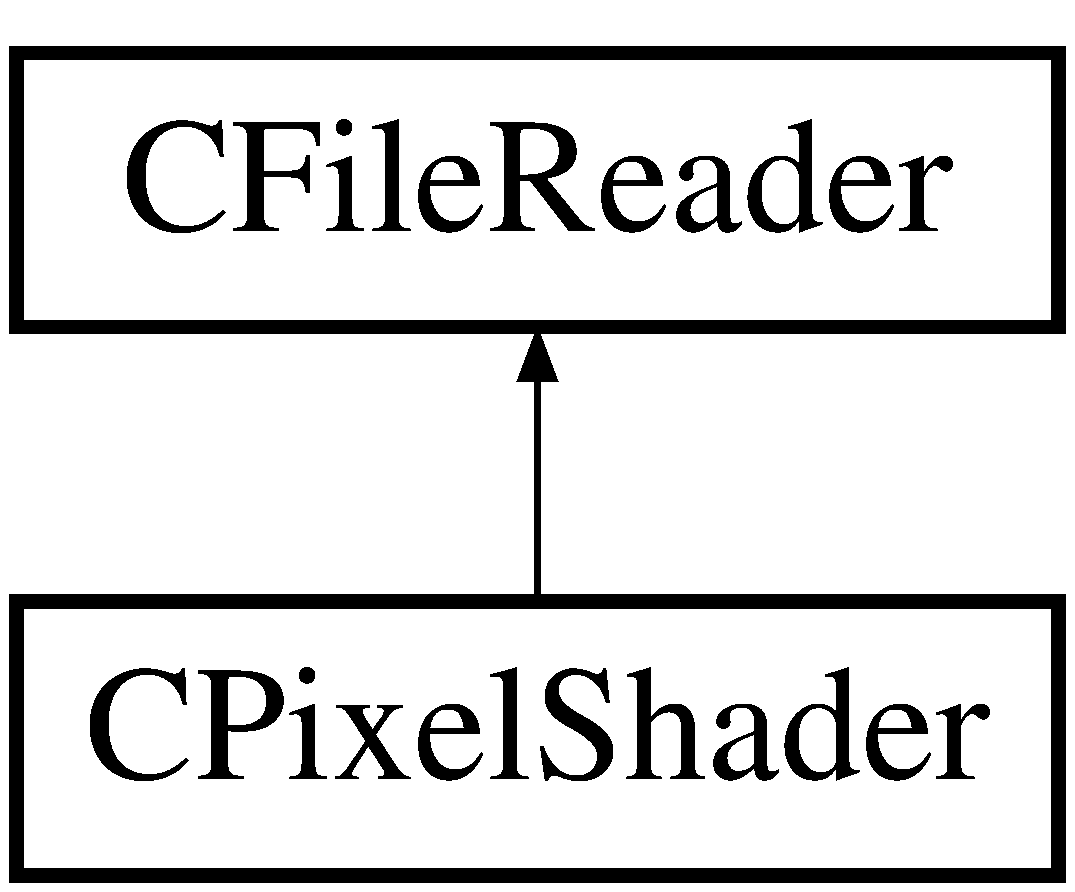
\includegraphics[height=2.000000cm]{class_c_pixel_shader}
\end{center}
\end{figure}
\subsection*{クラス}
\begin{DoxyCompactItemize}
\item 
struct \hyperlink{struct_c_pixel_shader_1_1_st_init_param}{St\+Init\+Param}
\begin{DoxyCompactList}\small\item\em 初期化用パラメータ。 \end{DoxyCompactList}\end{DoxyCompactItemize}
\subsection*{公開メンバ関数}
\begin{DoxyCompactItemize}
\item 
\hyperlink{class_c_pixel_shader_af98a997f879b9fc4f08affc2d1818bd1}{C\+Pixel\+Shader} (const \hyperlink{struct_c_pixel_shader_1_1_st_init_param}{St\+Init\+Param} \&\+\_\+rst\+Init\+Param)
\begin{DoxyCompactList}\small\item\em コンストラクタ。 \end{DoxyCompactList}\item 
virtual \hyperlink{class_c_pixel_shader_aad0c95b78a92ee366175157e09f6baea}{$\sim$\+C\+Pixel\+Shader} ()
\begin{DoxyCompactList}\small\item\em デストラクタ。 \end{DoxyCompactList}\item 
virtual void \hyperlink{class_c_pixel_shader_a5a70cfcd3b998c6f55f4c95f351e940e}{Read\+End\+Process} (const void $\ast$\+\_\+p\+Data, U\+Size \+\_\+u\+Size) override
\begin{DoxyCompactList}\small\item\em 読み込み完了時の処理。 \end{DoxyCompactList}\item 
I\+D3\+D\+Pixel\+Shader $\ast$ \hyperlink{class_c_pixel_shader_ad13d85569d067e80b15ddee8fd10e2a9}{Get\+Shader} () const 
\begin{DoxyCompactList}\small\item\em シェーダーを取得。 \end{DoxyCompactList}\end{DoxyCompactItemize}
\subsection*{非公開変数類}
\begin{DoxyCompactItemize}
\item 
I\+D3\+D\+Pixel\+Shader $\ast$ \hyperlink{class_c_pixel_shader_abd3ec734645bdd2d8828d30fad71ee4f}{m\+\_\+pc\+Pixel\+Shader}
\end{DoxyCompactItemize}


\subsection{構築子と解体子}
\hypertarget{class_c_pixel_shader_af98a997f879b9fc4f08affc2d1818bd1}{}\index{C\+Pixel\+Shader@{C\+Pixel\+Shader}!C\+Pixel\+Shader@{C\+Pixel\+Shader}}
\index{C\+Pixel\+Shader@{C\+Pixel\+Shader}!C\+Pixel\+Shader@{C\+Pixel\+Shader}}
\subsubsection[{C\+Pixel\+Shader(const St\+Init\+Param \&\+\_\+rst\+Init\+Param)}]{\setlength{\rightskip}{0pt plus 5cm}C\+Pixel\+Shader\+::\+C\+Pixel\+Shader (
\begin{DoxyParamCaption}
\item[{const {\bf St\+Init\+Param} \&}]{\+\_\+rst\+Init\+Param}
\end{DoxyParamCaption}
)}\label{class_c_pixel_shader_af98a997f879b9fc4f08affc2d1818bd1}


コンストラクタ。 


\begin{DoxyParams}[1]{引数}
\mbox{\tt in}  & {\em \+\_\+rst\+Init\+Param} & \+: 初期化用パラメータ。 \\
\hline
\end{DoxyParams}
\hypertarget{class_c_pixel_shader_aad0c95b78a92ee366175157e09f6baea}{}\index{C\+Pixel\+Shader@{C\+Pixel\+Shader}!````~C\+Pixel\+Shader@{$\sim$\+C\+Pixel\+Shader}}
\index{````~C\+Pixel\+Shader@{$\sim$\+C\+Pixel\+Shader}!C\+Pixel\+Shader@{C\+Pixel\+Shader}}
\subsubsection[{$\sim$\+C\+Pixel\+Shader()}]{\setlength{\rightskip}{0pt plus 5cm}C\+Pixel\+Shader\+::$\sim$\+C\+Pixel\+Shader (
\begin{DoxyParamCaption}
{}
\end{DoxyParamCaption}
)\hspace{0.3cm}{\ttfamily [virtual]}}\label{class_c_pixel_shader_aad0c95b78a92ee366175157e09f6baea}


デストラクタ。 



\subsection{関数詳解}
\hypertarget{class_c_pixel_shader_ad13d85569d067e80b15ddee8fd10e2a9}{}\index{C\+Pixel\+Shader@{C\+Pixel\+Shader}!Get\+Shader@{Get\+Shader}}
\index{Get\+Shader@{Get\+Shader}!C\+Pixel\+Shader@{C\+Pixel\+Shader}}
\subsubsection[{Get\+Shader() const }]{\setlength{\rightskip}{0pt plus 5cm}I\+D3\+D\+Pixel\+Shader$\ast$ C\+Pixel\+Shader\+::\+Get\+Shader (
\begin{DoxyParamCaption}
{}
\end{DoxyParamCaption}
) const\hspace{0.3cm}{\ttfamily [inline]}}\label{class_c_pixel_shader_ad13d85569d067e80b15ddee8fd10e2a9}


シェーダーを取得。 

\hypertarget{class_c_pixel_shader_a5a70cfcd3b998c6f55f4c95f351e940e}{}\index{C\+Pixel\+Shader@{C\+Pixel\+Shader}!Read\+End\+Process@{Read\+End\+Process}}
\index{Read\+End\+Process@{Read\+End\+Process}!C\+Pixel\+Shader@{C\+Pixel\+Shader}}
\subsubsection[{Read\+End\+Process(const void $\ast$\+\_\+p\+Data, U\+Size \+\_\+u\+Size) override}]{\setlength{\rightskip}{0pt plus 5cm}void C\+Pixel\+Shader\+::\+Read\+End\+Process (
\begin{DoxyParamCaption}
\item[{const void $\ast$}]{\+\_\+p\+Data, }
\item[{U\+Size}]{\+\_\+u\+Size}
\end{DoxyParamCaption}
)\hspace{0.3cm}{\ttfamily [override]}, {\ttfamily [virtual]}}\label{class_c_pixel_shader_a5a70cfcd3b998c6f55f4c95f351e940e}


読み込み完了時の処理。 


\begin{DoxyParams}[1]{引数}
\mbox{\tt in}  & {\em \+\_\+p\+Data} & \+: 読み込んだデータ。 \\
\hline
\mbox{\tt in}  & {\em \+\_\+u\+Size} & \+: 読み込んだデータサイズ。 \\
\hline
\end{DoxyParams}


\hyperlink{class_c_file_reader_a5a18550133826ac43096629f6eaa8c42}{C\+File\+Reader}を再実装しています。



\subsection{メンバ詳解}
\hypertarget{class_c_pixel_shader_abd3ec734645bdd2d8828d30fad71ee4f}{}\index{C\+Pixel\+Shader@{C\+Pixel\+Shader}!m\+\_\+pc\+Pixel\+Shader@{m\+\_\+pc\+Pixel\+Shader}}
\index{m\+\_\+pc\+Pixel\+Shader@{m\+\_\+pc\+Pixel\+Shader}!C\+Pixel\+Shader@{C\+Pixel\+Shader}}
\subsubsection[{m\+\_\+pc\+Pixel\+Shader}]{\setlength{\rightskip}{0pt plus 5cm}I\+D3\+D\+Pixel\+Shader$\ast$ C\+Pixel\+Shader\+::m\+\_\+pc\+Pixel\+Shader\hspace{0.3cm}{\ttfamily [private]}}\label{class_c_pixel_shader_abd3ec734645bdd2d8828d30fad71ee4f}


このクラス詳解は次のファイルから抽出されました\+:\begin{DoxyCompactItemize}
\item 
D\+:/\+Project/\+Game/\+Lib/\+Direct\+X/\hyperlink{_pixel_shader_8h}{Pixel\+Shader.\+h}\item 
D\+:/\+Project/\+Game/\+Lib/\+Direct\+X/\hyperlink{_pixel_shader_8cpp}{Pixel\+Shader.\+cpp}\end{DoxyCompactItemize}

\hypertarget{class_c_p_m_d_mesh}{}\section{C\+P\+M\+D\+Mesh クラス}
\label{class_c_p_m_d_mesh}\index{C\+P\+M\+D\+Mesh@{C\+P\+M\+D\+Mesh}}


{\ttfamily \#include $<$P\+M\+D\+Mesh.\+h$>$}

C\+P\+M\+D\+Mesh の継承関係図\begin{figure}[H]
\begin{center}
\leavevmode
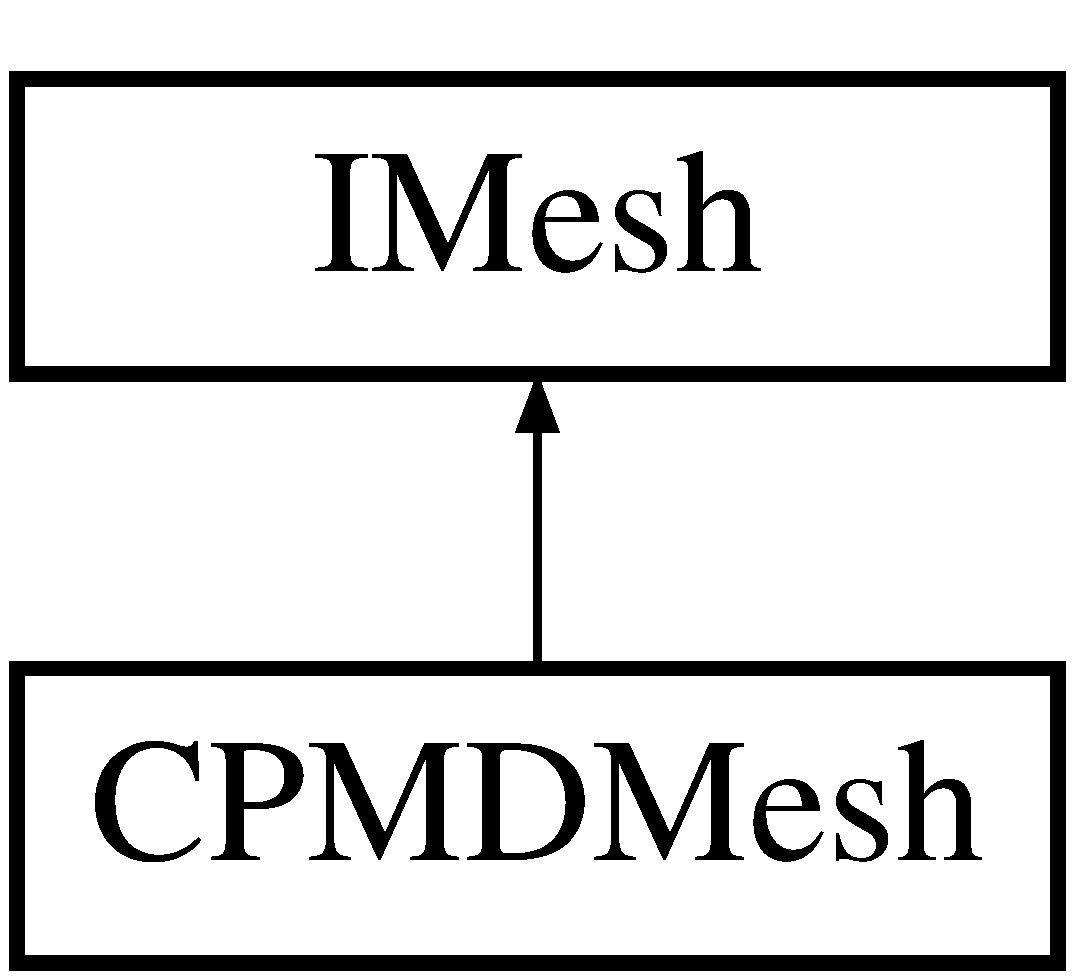
\includegraphics[height=2.000000cm]{class_c_p_m_d_mesh}
\end{center}
\end{figure}
\subsection*{公開メンバ関数}
\begin{DoxyCompactItemize}
\item 
\hyperlink{class_c_p_m_d_mesh_aa6c81a795b0497efecf17128385f853a}{C\+P\+M\+D\+Mesh} (const \hyperlink{class_c_p_m_d_reader}{C\+P\+M\+D\+Reader} \&\+\_\+rc\+Reader)
\begin{DoxyCompactList}\small\item\em コンストラクタ。 \end{DoxyCompactList}\item 
virtual \hyperlink{class_c_p_m_d_mesh_a5cd7433c40e72a8ac468e8fc248d49ce}{$\sim$\+C\+P\+M\+D\+Mesh} ()
\begin{DoxyCompactList}\small\item\em デストラクタ。 \end{DoxyCompactList}\item 
virtual U32 \hyperlink{class_c_p_m_d_mesh_a99a0e4d3664fae495cfe216170294aab}{Get\+Vertex\+Num} () const  override
\begin{DoxyCompactList}\small\item\em 頂点座標数を取得。 \end{DoxyCompactList}\item 
virtual const \hyperlink{struct_i_mesh_1_1_st_vertex}{St\+Vertex} $\ast$ \hyperlink{class_c_p_m_d_mesh_aa2b096b1102286fec5d8ea7cc381bb55}{Get\+Vertex\+Array} () const  override
\begin{DoxyCompactList}\small\item\em 頂点座標配列を取得。 \end{DoxyCompactList}\item 
virtual U32 \hyperlink{class_c_p_m_d_mesh_a0127281ef228e27dd6232069c5ffd164}{Get\+Index\+Num} () const  override
\begin{DoxyCompactList}\small\item\em インデックス数を取得。 \end{DoxyCompactList}\item 
virtual const U32 $\ast$ \hyperlink{class_c_p_m_d_mesh_ab2b12b75b3ed1ed3017cff8d52f1677b}{Get\+Index\+Array} () const  override
\begin{DoxyCompactList}\small\item\em インデックス配列を取得。 \end{DoxyCompactList}\item 
virtual U32 \hyperlink{class_c_p_m_d_mesh_a3dc32e47f692de7cc2c998b65a416c6d}{Get\+Material\+Num} () const  override
\begin{DoxyCompactList}\small\item\em マテリアル数を取得。 \end{DoxyCompactList}\item 
virtual const St\+Material $\ast$ \hyperlink{class_c_p_m_d_mesh_a8b6ba1255586f2387442ec24f92ade55}{Get\+Material\+Array} () const  override
\begin{DoxyCompactList}\small\item\em マテリアル配列を取得。 \end{DoxyCompactList}\end{DoxyCompactItemize}
\subsection*{非公開メンバ関数}
\begin{DoxyCompactItemize}
\item 
void \hyperlink{class_c_p_m_d_mesh_a3de096042308999ed7a2d37e66be76fc}{Extract\+Vertex} (const \hyperlink{class_c_p_m_d_reader}{C\+P\+M\+D\+Reader} \&\+\_\+rc\+Reader)
\begin{DoxyCompactList}\small\item\em 頂点情報を抽出。 \end{DoxyCompactList}\item 
void \hyperlink{class_c_p_m_d_mesh_a24efaf85ad9f3866a054d6a89b829612}{Extract\+Index} (const \hyperlink{class_c_p_m_d_reader}{C\+P\+M\+D\+Reader} \&\+\_\+rc\+Reader)
\begin{DoxyCompactList}\small\item\em インデック情報を抽出。 \end{DoxyCompactList}\item 
void \hyperlink{class_c_p_m_d_mesh_aeace2ace7326d12ee04f7549240c771e}{Extract\+Material} (const \hyperlink{class_c_p_m_d_reader}{C\+P\+M\+D\+Reader} \&\+\_\+rc\+Reader)
\begin{DoxyCompactList}\small\item\em マテリアル情報を抽出。 \end{DoxyCompactList}\end{DoxyCompactItemize}
\subsection*{非公開変数類}
\begin{DoxyCompactItemize}
\item 
U32 \hyperlink{class_c_p_m_d_mesh_a4f1ecf35269d6f92bdbb6a65fbcde9c7}{m\+\_\+u\+Vertex\+Num}
\begin{DoxyCompactList}\small\item\em 頂点情報数。 \end{DoxyCompactList}\item 
\hyperlink{struct_i_mesh_1_1_st_vertex}{St\+Vertex} $\ast$ \hyperlink{class_c_p_m_d_mesh_a3792b619ca88ed6376e3f13bad68309b}{m\+\_\+pst\+Vertex\+Array}
\begin{DoxyCompactList}\small\item\em 頂点情報配列。 \end{DoxyCompactList}\item 
U32 \hyperlink{class_c_p_m_d_mesh_a1bb03d6a05fcc301d52a683d435c0aca}{m\+\_\+u\+Index\+Num}
\begin{DoxyCompactList}\small\item\em インデックス数。 \end{DoxyCompactList}\item 
U32 $\ast$ \hyperlink{class_c_p_m_d_mesh_a2e6da3c8ef74817ba29900609ccd50a2}{m\+\_\+pu\+Index\+Array}
\begin{DoxyCompactList}\small\item\em インデック配列。 \end{DoxyCompactList}\item 
U32 \hyperlink{class_c_p_m_d_mesh_a90141785835f71c11ffe9146eecd1ff6}{m\+\_\+u\+Material\+Num}
\begin{DoxyCompactList}\small\item\em マテリアル数。 \end{DoxyCompactList}\item 
St\+Material $\ast$ \hyperlink{class_c_p_m_d_mesh_af1764e500e746f1271858e18b0e2a7bd}{m\+\_\+pst\+Material\+Array}
\begin{DoxyCompactList}\small\item\em マテリアル情報配列。 \end{DoxyCompactList}\end{DoxyCompactItemize}


\subsection{構築子と解体子}
\hypertarget{class_c_p_m_d_mesh_aa6c81a795b0497efecf17128385f853a}{}\index{C\+P\+M\+D\+Mesh@{C\+P\+M\+D\+Mesh}!C\+P\+M\+D\+Mesh@{C\+P\+M\+D\+Mesh}}
\index{C\+P\+M\+D\+Mesh@{C\+P\+M\+D\+Mesh}!C\+P\+M\+D\+Mesh@{C\+P\+M\+D\+Mesh}}
\subsubsection[{C\+P\+M\+D\+Mesh(const C\+P\+M\+D\+Reader \&\+\_\+rc\+Reader)}]{\setlength{\rightskip}{0pt plus 5cm}C\+P\+M\+D\+Mesh\+::\+C\+P\+M\+D\+Mesh (
\begin{DoxyParamCaption}
\item[{const {\bf C\+P\+M\+D\+Reader} \&}]{\+\_\+rc\+Reader}
\end{DoxyParamCaption}
)}\label{class_c_p_m_d_mesh_aa6c81a795b0497efecf17128385f853a}


コンストラクタ。 


\begin{DoxyParams}[1]{引数}
\mbox{\tt in}  & {\em \+\_\+rc\+Reader} & \+: P\+M\+D読み込みクラス。 \\
\hline
\end{DoxyParams}
\hypertarget{class_c_p_m_d_mesh_a5cd7433c40e72a8ac468e8fc248d49ce}{}\index{C\+P\+M\+D\+Mesh@{C\+P\+M\+D\+Mesh}!````~C\+P\+M\+D\+Mesh@{$\sim$\+C\+P\+M\+D\+Mesh}}
\index{````~C\+P\+M\+D\+Mesh@{$\sim$\+C\+P\+M\+D\+Mesh}!C\+P\+M\+D\+Mesh@{C\+P\+M\+D\+Mesh}}
\subsubsection[{$\sim$\+C\+P\+M\+D\+Mesh()}]{\setlength{\rightskip}{0pt plus 5cm}C\+P\+M\+D\+Mesh\+::$\sim$\+C\+P\+M\+D\+Mesh (
\begin{DoxyParamCaption}
{}
\end{DoxyParamCaption}
)\hspace{0.3cm}{\ttfamily [virtual]}}\label{class_c_p_m_d_mesh_a5cd7433c40e72a8ac468e8fc248d49ce}


デストラクタ。 



\subsection{関数詳解}
\hypertarget{class_c_p_m_d_mesh_a24efaf85ad9f3866a054d6a89b829612}{}\index{C\+P\+M\+D\+Mesh@{C\+P\+M\+D\+Mesh}!Extract\+Index@{Extract\+Index}}
\index{Extract\+Index@{Extract\+Index}!C\+P\+M\+D\+Mesh@{C\+P\+M\+D\+Mesh}}
\subsubsection[{Extract\+Index(const C\+P\+M\+D\+Reader \&\+\_\+rc\+Reader)}]{\setlength{\rightskip}{0pt plus 5cm}void C\+P\+M\+D\+Mesh\+::\+Extract\+Index (
\begin{DoxyParamCaption}
\item[{const {\bf C\+P\+M\+D\+Reader} \&}]{\+\_\+rc\+Reader}
\end{DoxyParamCaption}
)\hspace{0.3cm}{\ttfamily [private]}}\label{class_c_p_m_d_mesh_a24efaf85ad9f3866a054d6a89b829612}


インデック情報を抽出。 

インデックス情報を抽出。


\begin{DoxyParams}[1]{引数}
\mbox{\tt in}  & {\em \+\_\+rc\+Reader} & \+: P\+M\+D読み込みクラス。 \\
\hline
\end{DoxyParams}
\hypertarget{class_c_p_m_d_mesh_aeace2ace7326d12ee04f7549240c771e}{}\index{C\+P\+M\+D\+Mesh@{C\+P\+M\+D\+Mesh}!Extract\+Material@{Extract\+Material}}
\index{Extract\+Material@{Extract\+Material}!C\+P\+M\+D\+Mesh@{C\+P\+M\+D\+Mesh}}
\subsubsection[{Extract\+Material(const C\+P\+M\+D\+Reader \&\+\_\+rc\+Reader)}]{\setlength{\rightskip}{0pt plus 5cm}void C\+P\+M\+D\+Mesh\+::\+Extract\+Material (
\begin{DoxyParamCaption}
\item[{const {\bf C\+P\+M\+D\+Reader} \&}]{\+\_\+rc\+Reader}
\end{DoxyParamCaption}
)\hspace{0.3cm}{\ttfamily [private]}}\label{class_c_p_m_d_mesh_aeace2ace7326d12ee04f7549240c771e}


マテリアル情報を抽出。 


\begin{DoxyParams}[1]{引数}
\mbox{\tt in}  & {\em \+\_\+rc\+Reader} & \+: P\+M\+D読み込みクラス。 \\
\hline
\end{DoxyParams}
\hypertarget{class_c_p_m_d_mesh_a3de096042308999ed7a2d37e66be76fc}{}\index{C\+P\+M\+D\+Mesh@{C\+P\+M\+D\+Mesh}!Extract\+Vertex@{Extract\+Vertex}}
\index{Extract\+Vertex@{Extract\+Vertex}!C\+P\+M\+D\+Mesh@{C\+P\+M\+D\+Mesh}}
\subsubsection[{Extract\+Vertex(const C\+P\+M\+D\+Reader \&\+\_\+rc\+Reader)}]{\setlength{\rightskip}{0pt plus 5cm}void C\+P\+M\+D\+Mesh\+::\+Extract\+Vertex (
\begin{DoxyParamCaption}
\item[{const {\bf C\+P\+M\+D\+Reader} \&}]{\+\_\+rc\+Reader}
\end{DoxyParamCaption}
)\hspace{0.3cm}{\ttfamily [private]}}\label{class_c_p_m_d_mesh_a3de096042308999ed7a2d37e66be76fc}


頂点情報を抽出。 


\begin{DoxyParams}[1]{引数}
\mbox{\tt in}  & {\em \+\_\+rc\+Reader} & \+: P\+M\+D読み込みクラス。 \\
\hline
\end{DoxyParams}
\hypertarget{class_c_p_m_d_mesh_ab2b12b75b3ed1ed3017cff8d52f1677b}{}\index{C\+P\+M\+D\+Mesh@{C\+P\+M\+D\+Mesh}!Get\+Index\+Array@{Get\+Index\+Array}}
\index{Get\+Index\+Array@{Get\+Index\+Array}!C\+P\+M\+D\+Mesh@{C\+P\+M\+D\+Mesh}}
\subsubsection[{Get\+Index\+Array() const  override}]{\setlength{\rightskip}{0pt plus 5cm}virtual const U32$\ast$ C\+P\+M\+D\+Mesh\+::\+Get\+Index\+Array (
\begin{DoxyParamCaption}
{}
\end{DoxyParamCaption}
) const\hspace{0.3cm}{\ttfamily [inline]}, {\ttfamily [override]}, {\ttfamily [virtual]}}\label{class_c_p_m_d_mesh_ab2b12b75b3ed1ed3017cff8d52f1677b}


インデックス配列を取得。 



\hyperlink{class_i_mesh_a3a9e9207cfae24ae1dd62eb2d2356301}{I\+Mesh}を実装しています。

\hypertarget{class_c_p_m_d_mesh_a0127281ef228e27dd6232069c5ffd164}{}\index{C\+P\+M\+D\+Mesh@{C\+P\+M\+D\+Mesh}!Get\+Index\+Num@{Get\+Index\+Num}}
\index{Get\+Index\+Num@{Get\+Index\+Num}!C\+P\+M\+D\+Mesh@{C\+P\+M\+D\+Mesh}}
\subsubsection[{Get\+Index\+Num() const  override}]{\setlength{\rightskip}{0pt plus 5cm}virtual U32 C\+P\+M\+D\+Mesh\+::\+Get\+Index\+Num (
\begin{DoxyParamCaption}
{}
\end{DoxyParamCaption}
) const\hspace{0.3cm}{\ttfamily [inline]}, {\ttfamily [override]}, {\ttfamily [virtual]}}\label{class_c_p_m_d_mesh_a0127281ef228e27dd6232069c5ffd164}


インデックス数を取得。 



\hyperlink{class_i_mesh_a580358c71d8766c1e0aa8037b51a9296}{I\+Mesh}を実装しています。

\hypertarget{class_c_p_m_d_mesh_a8b6ba1255586f2387442ec24f92ade55}{}\index{C\+P\+M\+D\+Mesh@{C\+P\+M\+D\+Mesh}!Get\+Material\+Array@{Get\+Material\+Array}}
\index{Get\+Material\+Array@{Get\+Material\+Array}!C\+P\+M\+D\+Mesh@{C\+P\+M\+D\+Mesh}}
\subsubsection[{Get\+Material\+Array() const  override}]{\setlength{\rightskip}{0pt plus 5cm}virtual const St\+Material$\ast$ C\+P\+M\+D\+Mesh\+::\+Get\+Material\+Array (
\begin{DoxyParamCaption}
{}
\end{DoxyParamCaption}
) const\hspace{0.3cm}{\ttfamily [inline]}, {\ttfamily [override]}, {\ttfamily [virtual]}}\label{class_c_p_m_d_mesh_a8b6ba1255586f2387442ec24f92ade55}


マテリアル配列を取得。 



\hyperlink{class_i_mesh_a48afb85120e333b50ac9de73b8b60d16}{I\+Mesh}を実装しています。

\hypertarget{class_c_p_m_d_mesh_a3dc32e47f692de7cc2c998b65a416c6d}{}\index{C\+P\+M\+D\+Mesh@{C\+P\+M\+D\+Mesh}!Get\+Material\+Num@{Get\+Material\+Num}}
\index{Get\+Material\+Num@{Get\+Material\+Num}!C\+P\+M\+D\+Mesh@{C\+P\+M\+D\+Mesh}}
\subsubsection[{Get\+Material\+Num() const  override}]{\setlength{\rightskip}{0pt plus 5cm}virtual U32 C\+P\+M\+D\+Mesh\+::\+Get\+Material\+Num (
\begin{DoxyParamCaption}
{}
\end{DoxyParamCaption}
) const\hspace{0.3cm}{\ttfamily [inline]}, {\ttfamily [override]}, {\ttfamily [virtual]}}\label{class_c_p_m_d_mesh_a3dc32e47f692de7cc2c998b65a416c6d}


マテリアル数を取得。 



\hyperlink{class_i_mesh_a1b8922bc90cd0951062053e24287ad6c}{I\+Mesh}を実装しています。

\hypertarget{class_c_p_m_d_mesh_aa2b096b1102286fec5d8ea7cc381bb55}{}\index{C\+P\+M\+D\+Mesh@{C\+P\+M\+D\+Mesh}!Get\+Vertex\+Array@{Get\+Vertex\+Array}}
\index{Get\+Vertex\+Array@{Get\+Vertex\+Array}!C\+P\+M\+D\+Mesh@{C\+P\+M\+D\+Mesh}}
\subsubsection[{Get\+Vertex\+Array() const  override}]{\setlength{\rightskip}{0pt plus 5cm}virtual const {\bf St\+Vertex}$\ast$ C\+P\+M\+D\+Mesh\+::\+Get\+Vertex\+Array (
\begin{DoxyParamCaption}
{}
\end{DoxyParamCaption}
) const\hspace{0.3cm}{\ttfamily [inline]}, {\ttfamily [override]}, {\ttfamily [virtual]}}\label{class_c_p_m_d_mesh_aa2b096b1102286fec5d8ea7cc381bb55}


頂点座標配列を取得。 



\hyperlink{class_i_mesh_a91d4b99a5a91cb54d364cc6a8342b187}{I\+Mesh}を実装しています。

\hypertarget{class_c_p_m_d_mesh_a99a0e4d3664fae495cfe216170294aab}{}\index{C\+P\+M\+D\+Mesh@{C\+P\+M\+D\+Mesh}!Get\+Vertex\+Num@{Get\+Vertex\+Num}}
\index{Get\+Vertex\+Num@{Get\+Vertex\+Num}!C\+P\+M\+D\+Mesh@{C\+P\+M\+D\+Mesh}}
\subsubsection[{Get\+Vertex\+Num() const  override}]{\setlength{\rightskip}{0pt plus 5cm}virtual U32 C\+P\+M\+D\+Mesh\+::\+Get\+Vertex\+Num (
\begin{DoxyParamCaption}
{}
\end{DoxyParamCaption}
) const\hspace{0.3cm}{\ttfamily [inline]}, {\ttfamily [override]}, {\ttfamily [virtual]}}\label{class_c_p_m_d_mesh_a99a0e4d3664fae495cfe216170294aab}


頂点座標数を取得。 



\hyperlink{class_i_mesh_a98ac2c9b1da3c22191e4198833a4f6ef}{I\+Mesh}を実装しています。



\subsection{メンバ詳解}
\hypertarget{class_c_p_m_d_mesh_af1764e500e746f1271858e18b0e2a7bd}{}\index{C\+P\+M\+D\+Mesh@{C\+P\+M\+D\+Mesh}!m\+\_\+pst\+Material\+Array@{m\+\_\+pst\+Material\+Array}}
\index{m\+\_\+pst\+Material\+Array@{m\+\_\+pst\+Material\+Array}!C\+P\+M\+D\+Mesh@{C\+P\+M\+D\+Mesh}}
\subsubsection[{m\+\_\+pst\+Material\+Array}]{\setlength{\rightskip}{0pt plus 5cm}St\+Material$\ast$ C\+P\+M\+D\+Mesh\+::m\+\_\+pst\+Material\+Array\hspace{0.3cm}{\ttfamily [private]}}\label{class_c_p_m_d_mesh_af1764e500e746f1271858e18b0e2a7bd}


マテリアル情報配列。 

\hypertarget{class_c_p_m_d_mesh_a3792b619ca88ed6376e3f13bad68309b}{}\index{C\+P\+M\+D\+Mesh@{C\+P\+M\+D\+Mesh}!m\+\_\+pst\+Vertex\+Array@{m\+\_\+pst\+Vertex\+Array}}
\index{m\+\_\+pst\+Vertex\+Array@{m\+\_\+pst\+Vertex\+Array}!C\+P\+M\+D\+Mesh@{C\+P\+M\+D\+Mesh}}
\subsubsection[{m\+\_\+pst\+Vertex\+Array}]{\setlength{\rightskip}{0pt plus 5cm}{\bf St\+Vertex}$\ast$ C\+P\+M\+D\+Mesh\+::m\+\_\+pst\+Vertex\+Array\hspace{0.3cm}{\ttfamily [private]}}\label{class_c_p_m_d_mesh_a3792b619ca88ed6376e3f13bad68309b}


頂点情報配列。 

\hypertarget{class_c_p_m_d_mesh_a2e6da3c8ef74817ba29900609ccd50a2}{}\index{C\+P\+M\+D\+Mesh@{C\+P\+M\+D\+Mesh}!m\+\_\+pu\+Index\+Array@{m\+\_\+pu\+Index\+Array}}
\index{m\+\_\+pu\+Index\+Array@{m\+\_\+pu\+Index\+Array}!C\+P\+M\+D\+Mesh@{C\+P\+M\+D\+Mesh}}
\subsubsection[{m\+\_\+pu\+Index\+Array}]{\setlength{\rightskip}{0pt plus 5cm}U32$\ast$ C\+P\+M\+D\+Mesh\+::m\+\_\+pu\+Index\+Array\hspace{0.3cm}{\ttfamily [private]}}\label{class_c_p_m_d_mesh_a2e6da3c8ef74817ba29900609ccd50a2}


インデック配列。 

\hypertarget{class_c_p_m_d_mesh_a1bb03d6a05fcc301d52a683d435c0aca}{}\index{C\+P\+M\+D\+Mesh@{C\+P\+M\+D\+Mesh}!m\+\_\+u\+Index\+Num@{m\+\_\+u\+Index\+Num}}
\index{m\+\_\+u\+Index\+Num@{m\+\_\+u\+Index\+Num}!C\+P\+M\+D\+Mesh@{C\+P\+M\+D\+Mesh}}
\subsubsection[{m\+\_\+u\+Index\+Num}]{\setlength{\rightskip}{0pt plus 5cm}U32 C\+P\+M\+D\+Mesh\+::m\+\_\+u\+Index\+Num\hspace{0.3cm}{\ttfamily [private]}}\label{class_c_p_m_d_mesh_a1bb03d6a05fcc301d52a683d435c0aca}


インデックス数。 

\hypertarget{class_c_p_m_d_mesh_a90141785835f71c11ffe9146eecd1ff6}{}\index{C\+P\+M\+D\+Mesh@{C\+P\+M\+D\+Mesh}!m\+\_\+u\+Material\+Num@{m\+\_\+u\+Material\+Num}}
\index{m\+\_\+u\+Material\+Num@{m\+\_\+u\+Material\+Num}!C\+P\+M\+D\+Mesh@{C\+P\+M\+D\+Mesh}}
\subsubsection[{m\+\_\+u\+Material\+Num}]{\setlength{\rightskip}{0pt plus 5cm}U32 C\+P\+M\+D\+Mesh\+::m\+\_\+u\+Material\+Num\hspace{0.3cm}{\ttfamily [private]}}\label{class_c_p_m_d_mesh_a90141785835f71c11ffe9146eecd1ff6}


マテリアル数。 

\hypertarget{class_c_p_m_d_mesh_a4f1ecf35269d6f92bdbb6a65fbcde9c7}{}\index{C\+P\+M\+D\+Mesh@{C\+P\+M\+D\+Mesh}!m\+\_\+u\+Vertex\+Num@{m\+\_\+u\+Vertex\+Num}}
\index{m\+\_\+u\+Vertex\+Num@{m\+\_\+u\+Vertex\+Num}!C\+P\+M\+D\+Mesh@{C\+P\+M\+D\+Mesh}}
\subsubsection[{m\+\_\+u\+Vertex\+Num}]{\setlength{\rightskip}{0pt plus 5cm}U32 C\+P\+M\+D\+Mesh\+::m\+\_\+u\+Vertex\+Num\hspace{0.3cm}{\ttfamily [private]}}\label{class_c_p_m_d_mesh_a4f1ecf35269d6f92bdbb6a65fbcde9c7}


頂点情報数。 



このクラス詳解は次のファイルから抽出されました\+:\begin{DoxyCompactItemize}
\item 
D\+:/\+Project/\+Game/\+Lib/\+P\+M\+D/\hyperlink{_p_m_d_mesh_8h}{P\+M\+D\+Mesh.\+h}\item 
D\+:/\+Project/\+Game/\+Lib/\+P\+M\+D/\hyperlink{_p_m_d_mesh_8cpp}{P\+M\+D\+Mesh.\+cpp}\end{DoxyCompactItemize}

\hypertarget{class_c_p_m_d_reader}{}\section{C\+P\+M\+D\+Reader クラス}
\label{class_c_p_m_d_reader}\index{C\+P\+M\+D\+Reader@{C\+P\+M\+D\+Reader}}


{\ttfamily \#include $<$P\+M\+D\+Reader.\+h$>$}

C\+P\+M\+D\+Reader の継承関係図\begin{figure}[H]
\begin{center}
\leavevmode
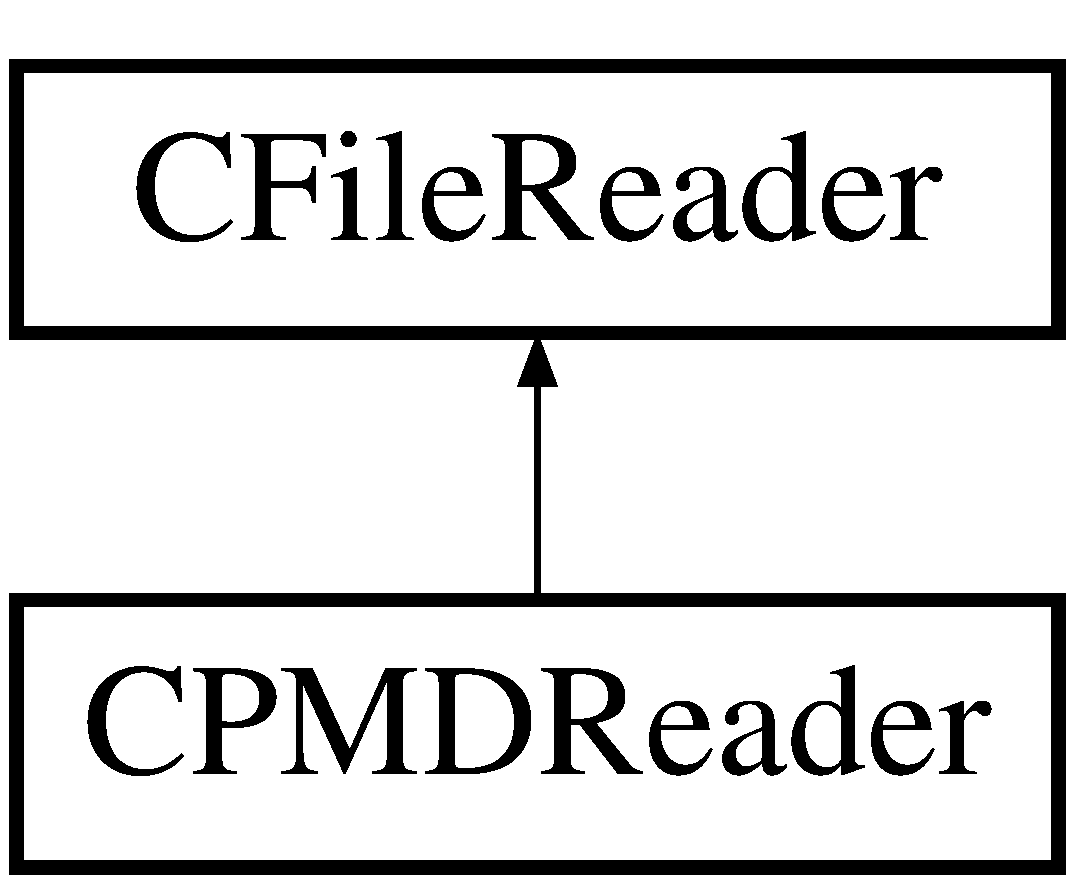
\includegraphics[height=2.000000cm]{class_c_p_m_d_reader}
\end{center}
\end{figure}
\subsection*{公開メンバ関数}
\begin{DoxyCompactItemize}
\item 
\hyperlink{class_c_p_m_d_reader_a8d2c4bdfa2c288fe4d3507a26c7f13a7}{C\+P\+M\+D\+Reader} (const T\+Char $\ast$\+\_\+ps\+File\+Name)
\begin{DoxyCompactList}\small\item\em コンストラクタ。 \end{DoxyCompactList}\item 
virtual \hyperlink{class_c_p_m_d_reader_a3e1afba2bd86e420c731ba5c114d2ec5}{$\sim$\+C\+P\+M\+D\+Reader} ()
\begin{DoxyCompactList}\small\item\em デストラクタ。 \end{DoxyCompactList}\item 
virtual void \hyperlink{class_c_p_m_d_reader_a326af26b1815aaa4b088b037fb76e05f}{Read\+End\+Process} (const void $\ast$\+\_\+p\+Data, U\+Size \+\_\+u\+Size) override
\begin{DoxyCompactList}\small\item\em 読み込み完了時の処理。 \end{DoxyCompactList}\item 
const meshio\+::pmd\+::\+I\+O \& \hyperlink{class_c_p_m_d_reader_a082ea64273d18d684b3fc2deced6090f}{Get\+P\+M\+D\+Data} () const 
\begin{DoxyCompactList}\small\item\em P\+M\+Dデータの取得。 \end{DoxyCompactList}\end{DoxyCompactItemize}
\subsection*{非公開変数類}
\begin{DoxyCompactItemize}
\item 
meshio\+::pmd\+::\+I\+O \hyperlink{class_c_p_m_d_reader_aaecdb1ffd39ffe2cb5c87597c581173f}{m\+\_\+st\+Data}
\end{DoxyCompactItemize}


\subsection{構築子と解体子}
\hypertarget{class_c_p_m_d_reader_a8d2c4bdfa2c288fe4d3507a26c7f13a7}{}\index{C\+P\+M\+D\+Reader@{C\+P\+M\+D\+Reader}!C\+P\+M\+D\+Reader@{C\+P\+M\+D\+Reader}}
\index{C\+P\+M\+D\+Reader@{C\+P\+M\+D\+Reader}!C\+P\+M\+D\+Reader@{C\+P\+M\+D\+Reader}}
\subsubsection[{C\+P\+M\+D\+Reader(const T\+Char $\ast$\+\_\+ps\+File\+Name)}]{\setlength{\rightskip}{0pt plus 5cm}C\+P\+M\+D\+Reader\+::\+C\+P\+M\+D\+Reader (
\begin{DoxyParamCaption}
\item[{const T\+Char $\ast$}]{\+\_\+ps\+File\+Name}
\end{DoxyParamCaption}
)}\label{class_c_p_m_d_reader_a8d2c4bdfa2c288fe4d3507a26c7f13a7}


コンストラクタ。 


\begin{DoxyParams}[1]{引数}
\mbox{\tt in}  & {\em \+\_\+ps\+File\+Name} & \+: 読み込むファイル名。 \\
\hline
\end{DoxyParams}
\hypertarget{class_c_p_m_d_reader_a3e1afba2bd86e420c731ba5c114d2ec5}{}\index{C\+P\+M\+D\+Reader@{C\+P\+M\+D\+Reader}!````~C\+P\+M\+D\+Reader@{$\sim$\+C\+P\+M\+D\+Reader}}
\index{````~C\+P\+M\+D\+Reader@{$\sim$\+C\+P\+M\+D\+Reader}!C\+P\+M\+D\+Reader@{C\+P\+M\+D\+Reader}}
\subsubsection[{$\sim$\+C\+P\+M\+D\+Reader()}]{\setlength{\rightskip}{0pt plus 5cm}C\+P\+M\+D\+Reader\+::$\sim$\+C\+P\+M\+D\+Reader (
\begin{DoxyParamCaption}
{}
\end{DoxyParamCaption}
)\hspace{0.3cm}{\ttfamily [virtual]}}\label{class_c_p_m_d_reader_a3e1afba2bd86e420c731ba5c114d2ec5}


デストラクタ。 



\subsection{関数詳解}
\hypertarget{class_c_p_m_d_reader_a082ea64273d18d684b3fc2deced6090f}{}\index{C\+P\+M\+D\+Reader@{C\+P\+M\+D\+Reader}!Get\+P\+M\+D\+Data@{Get\+P\+M\+D\+Data}}
\index{Get\+P\+M\+D\+Data@{Get\+P\+M\+D\+Data}!C\+P\+M\+D\+Reader@{C\+P\+M\+D\+Reader}}
\subsubsection[{Get\+P\+M\+D\+Data() const }]{\setlength{\rightskip}{0pt plus 5cm}const meshio\+::pmd\+::\+I\+O\& C\+P\+M\+D\+Reader\+::\+Get\+P\+M\+D\+Data (
\begin{DoxyParamCaption}
{}
\end{DoxyParamCaption}
) const\hspace{0.3cm}{\ttfamily [inline]}}\label{class_c_p_m_d_reader_a082ea64273d18d684b3fc2deced6090f}


P\+M\+Dデータの取得。 

\hypertarget{class_c_p_m_d_reader_a326af26b1815aaa4b088b037fb76e05f}{}\index{C\+P\+M\+D\+Reader@{C\+P\+M\+D\+Reader}!Read\+End\+Process@{Read\+End\+Process}}
\index{Read\+End\+Process@{Read\+End\+Process}!C\+P\+M\+D\+Reader@{C\+P\+M\+D\+Reader}}
\subsubsection[{Read\+End\+Process(const void $\ast$\+\_\+p\+Data, U\+Size \+\_\+u\+Size) override}]{\setlength{\rightskip}{0pt plus 5cm}void C\+P\+M\+D\+Reader\+::\+Read\+End\+Process (
\begin{DoxyParamCaption}
\item[{const void $\ast$}]{\+\_\+p\+Data, }
\item[{U\+Size}]{\+\_\+u\+Size}
\end{DoxyParamCaption}
)\hspace{0.3cm}{\ttfamily [override]}, {\ttfamily [virtual]}}\label{class_c_p_m_d_reader_a326af26b1815aaa4b088b037fb76e05f}


読み込み完了時の処理。 


\begin{DoxyParams}[1]{引数}
\mbox{\tt in}  & {\em \+\_\+p\+Data} & \+: 読み込んだデータ。 \\
\hline
\mbox{\tt in}  & {\em \+\_\+u\+Size} & \+: データサイズ。 \\
\hline
\end{DoxyParams}


\hyperlink{class_c_file_reader_a5a18550133826ac43096629f6eaa8c42}{C\+File\+Reader}を再実装しています。



\subsection{メンバ詳解}
\hypertarget{class_c_p_m_d_reader_aaecdb1ffd39ffe2cb5c87597c581173f}{}\index{C\+P\+M\+D\+Reader@{C\+P\+M\+D\+Reader}!m\+\_\+st\+Data@{m\+\_\+st\+Data}}
\index{m\+\_\+st\+Data@{m\+\_\+st\+Data}!C\+P\+M\+D\+Reader@{C\+P\+M\+D\+Reader}}
\subsubsection[{m\+\_\+st\+Data}]{\setlength{\rightskip}{0pt plus 5cm}meshio\+::pmd\+::\+I\+O C\+P\+M\+D\+Reader\+::m\+\_\+st\+Data\hspace{0.3cm}{\ttfamily [private]}}\label{class_c_p_m_d_reader_aaecdb1ffd39ffe2cb5c87597c581173f}


このクラス詳解は次のファイルから抽出されました\+:\begin{DoxyCompactItemize}
\item 
D\+:/\+Project/\+Game/\+Lib/\+P\+M\+D/\hyperlink{_p_m_d_reader_8h}{P\+M\+D\+Reader.\+h}\item 
D\+:/\+Project/\+Game/\+Lib/\+P\+M\+D/\hyperlink{_p_m_d_reader_8cpp}{P\+M\+D\+Reader.\+cpp}\end{DoxyCompactItemize}

\hypertarget{class_c_random_int}{}\section{C\+Random\+Int$<$ T $>$ クラステンプレート}
\label{class_c_random_int}\index{C\+Random\+Int$<$ T $>$@{C\+Random\+Int$<$ T $>$}}


{\ttfamily \#include $<$Random.\+h$>$}

\subsection*{公開メンバ関数}
\begin{DoxyCompactItemize}
\item 
\hyperlink{class_c_random_int_a5f3ff4ea24378926da8aac150a4a33fd}{C\+Random\+Int} (T \+\_\+f\+Min, T \+\_\+f\+Max)
\begin{DoxyCompactList}\small\item\em コンストラクタ。 \end{DoxyCompactList}\item 
\hyperlink{class_c_random_int_a7cc41c7e1b21a16a8bfe3c79bb665e22}{$\sim$\+C\+Random\+Int} ()
\begin{DoxyCompactList}\small\item\em デストラクタ。 \end{DoxyCompactList}\item 
T \hyperlink{class_c_random_int_a04dfe95f084771d7c0392eef857f27ff}{Get\+Random} ()
\begin{DoxyCompactList}\small\item\em 乱数を取得。 \end{DoxyCompactList}\end{DoxyCompactItemize}
\subsection*{非公開変数類}
\begin{DoxyCompactItemize}
\item 
std\+::mt19937\+\_\+64 $\ast$ \hyperlink{class_c_random_int_aae181316633165d9888d530e15f8232b}{m\+\_\+pc\+Random\+M\+T}
\begin{DoxyCompactList}\small\item\em メルセンヌ・ツイスター法による乱数生成。 \end{DoxyCompactList}\item 
std\+::uniform\+\_\+int\+\_\+distribution$<$ T $>$ $\ast$ \hyperlink{class_c_random_int_a5c6565335676d670c0072236d18e34cc}{m\+\_\+pc\+Distribution}
\end{DoxyCompactItemize}


\subsection{構築子と解体子}
\hypertarget{class_c_random_int_a5f3ff4ea24378926da8aac150a4a33fd}{}\index{C\+Random\+Int@{C\+Random\+Int}!C\+Random\+Int@{C\+Random\+Int}}
\index{C\+Random\+Int@{C\+Random\+Int}!C\+Random\+Int@{C\+Random\+Int}}
\subsubsection[{C\+Random\+Int(\+T \+\_\+f\+Min, T \+\_\+f\+Max)}]{\setlength{\rightskip}{0pt plus 5cm}template$<$typename T $>$ {\bf C\+Random\+Int}$<$ T $>$\+::{\bf C\+Random\+Int} (
\begin{DoxyParamCaption}
\item[{T}]{\+\_\+f\+Min, }
\item[{T}]{\+\_\+f\+Max}
\end{DoxyParamCaption}
)}\label{class_c_random_int_a5f3ff4ea24378926da8aac150a4a33fd}


コンストラクタ。 


\begin{DoxyParams}[1]{引数}
\mbox{\tt in}  & {\em \+\_\+f\+Min} & \+: 乱数の最小値。 \\
\hline
\mbox{\tt in}  & {\em \+\_\+f\+Max} & \+: 乱数の最大値。 \\
\hline
\end{DoxyParams}
\hypertarget{class_c_random_int_a7cc41c7e1b21a16a8bfe3c79bb665e22}{}\index{C\+Random\+Int@{C\+Random\+Int}!````~C\+Random\+Int@{$\sim$\+C\+Random\+Int}}
\index{````~C\+Random\+Int@{$\sim$\+C\+Random\+Int}!C\+Random\+Int@{C\+Random\+Int}}
\subsubsection[{$\sim$\+C\+Random\+Int()}]{\setlength{\rightskip}{0pt plus 5cm}template$<$typename T $>$ {\bf C\+Random\+Int}$<$ T $>$\+::$\sim${\bf C\+Random\+Int} (
\begin{DoxyParamCaption}
{}
\end{DoxyParamCaption}
)}\label{class_c_random_int_a7cc41c7e1b21a16a8bfe3c79bb665e22}


デストラクタ。 



\subsection{関数詳解}
\hypertarget{class_c_random_int_a04dfe95f084771d7c0392eef857f27ff}{}\index{C\+Random\+Int@{C\+Random\+Int}!Get\+Random@{Get\+Random}}
\index{Get\+Random@{Get\+Random}!C\+Random\+Int@{C\+Random\+Int}}
\subsubsection[{Get\+Random()}]{\setlength{\rightskip}{0pt plus 5cm}template$<$typename T $>$ T {\bf C\+Random\+Int}$<$ T $>$\+::Get\+Random (
\begin{DoxyParamCaption}
{}
\end{DoxyParamCaption}
)}\label{class_c_random_int_a04dfe95f084771d7c0392eef857f27ff}


乱数を取得。 


\begin{DoxyRetVals}{戻り値}
{\em コンストラクタで指定した範囲内の乱数。} & \\
\hline
\end{DoxyRetVals}


\subsection{メンバ詳解}
\hypertarget{class_c_random_int_a5c6565335676d670c0072236d18e34cc}{}\index{C\+Random\+Int@{C\+Random\+Int}!m\+\_\+pc\+Distribution@{m\+\_\+pc\+Distribution}}
\index{m\+\_\+pc\+Distribution@{m\+\_\+pc\+Distribution}!C\+Random\+Int@{C\+Random\+Int}}
\subsubsection[{m\+\_\+pc\+Distribution}]{\setlength{\rightskip}{0pt plus 5cm}template$<$typename T $>$ std\+::uniform\+\_\+int\+\_\+distribution$<$T$>$$\ast$ {\bf C\+Random\+Int}$<$ T $>$\+::m\+\_\+pc\+Distribution\hspace{0.3cm}{\ttfamily [private]}}\label{class_c_random_int_a5c6565335676d670c0072236d18e34cc}
\hypertarget{class_c_random_int_aae181316633165d9888d530e15f8232b}{}\index{C\+Random\+Int@{C\+Random\+Int}!m\+\_\+pc\+Random\+M\+T@{m\+\_\+pc\+Random\+M\+T}}
\index{m\+\_\+pc\+Random\+M\+T@{m\+\_\+pc\+Random\+M\+T}!C\+Random\+Int@{C\+Random\+Int}}
\subsubsection[{m\+\_\+pc\+Random\+M\+T}]{\setlength{\rightskip}{0pt plus 5cm}template$<$typename T $>$ std\+::mt19937\+\_\+64$\ast$ {\bf C\+Random\+Int}$<$ T $>$\+::m\+\_\+pc\+Random\+M\+T\hspace{0.3cm}{\ttfamily [private]}}\label{class_c_random_int_aae181316633165d9888d530e15f8232b}


メルセンヌ・ツイスター法による乱数生成。 



このクラス詳解は次のファイルから抽出されました\+:\begin{DoxyCompactItemize}
\item 
D\+:/\+Project/\+Game/\+Lib/\+Random/\hyperlink{_random_8h}{Random.\+h}\item 
D\+:/\+Project/\+Game/\+Lib/\+Random/\hyperlink{_random_int_8h}{Random\+Int.\+h}\end{DoxyCompactItemize}

\hypertarget{class_c_random_real}{}\section{C\+Random\+Real$<$ T $>$ クラステンプレート}
\label{class_c_random_real}\index{C\+Random\+Real$<$ T $>$@{C\+Random\+Real$<$ T $>$}}


{\ttfamily \#include $<$Random.\+h$>$}

\subsection*{公開メンバ関数}
\begin{DoxyCompactItemize}
\item 
\hyperlink{class_c_random_real_ae4e392ce256d39dd23efd10bb854497b}{C\+Random\+Real} (T \+\_\+f\+Min, T \+\_\+f\+Max)
\begin{DoxyCompactList}\small\item\em コンストラクタ。 \end{DoxyCompactList}\item 
\hyperlink{class_c_random_real_a1816488bda25256c76f4c1398813789a}{$\sim$\+C\+Random\+Real} ()
\begin{DoxyCompactList}\small\item\em デストラクタ。 \end{DoxyCompactList}\item 
T \hyperlink{class_c_random_real_a9c2371d1a531aa18ce4f448fe9c762f6}{Get\+Random} ()
\begin{DoxyCompactList}\small\item\em 乱数を取得。 \end{DoxyCompactList}\end{DoxyCompactItemize}
\subsection*{非公開変数類}
\begin{DoxyCompactItemize}
\item 
std\+::mt19937\+\_\+64 $\ast$ \hyperlink{class_c_random_real_a037817cfa9e79313ea851b03fa1fd4ad}{m\+\_\+pc\+Random\+M\+T}
\begin{DoxyCompactList}\small\item\em メルセンヌ・ツイスター法による乱数生成。 \end{DoxyCompactList}\item 
std\+::uniform\+\_\+real\+\_\+distribution$<$ T $>$ $\ast$ \hyperlink{class_c_random_real_a2cf71bd4ff15374b9b079b38125867e3}{m\+\_\+pc\+Distribution}
\end{DoxyCompactItemize}


\subsection{構築子と解体子}
\hypertarget{class_c_random_real_ae4e392ce256d39dd23efd10bb854497b}{}\index{C\+Random\+Real@{C\+Random\+Real}!C\+Random\+Real@{C\+Random\+Real}}
\index{C\+Random\+Real@{C\+Random\+Real}!C\+Random\+Real@{C\+Random\+Real}}
\subsubsection[{C\+Random\+Real(\+T \+\_\+f\+Min, T \+\_\+f\+Max)}]{\setlength{\rightskip}{0pt plus 5cm}template$<$typename T $>$ {\bf C\+Random\+Real}$<$ T $>$\+::{\bf C\+Random\+Real} (
\begin{DoxyParamCaption}
\item[{T}]{\+\_\+f\+Min, }
\item[{T}]{\+\_\+f\+Max}
\end{DoxyParamCaption}
)}\label{class_c_random_real_ae4e392ce256d39dd23efd10bb854497b}


コンストラクタ。 


\begin{DoxyParams}[1]{引数}
\mbox{\tt in}  & {\em \+\_\+f\+Min} & \+: 乱数の最小値。 \\
\hline
\mbox{\tt in}  & {\em \+\_\+f\+Max} & \+: 乱数の最大値。 \\
\hline
\end{DoxyParams}
\hypertarget{class_c_random_real_a1816488bda25256c76f4c1398813789a}{}\index{C\+Random\+Real@{C\+Random\+Real}!````~C\+Random\+Real@{$\sim$\+C\+Random\+Real}}
\index{````~C\+Random\+Real@{$\sim$\+C\+Random\+Real}!C\+Random\+Real@{C\+Random\+Real}}
\subsubsection[{$\sim$\+C\+Random\+Real()}]{\setlength{\rightskip}{0pt plus 5cm}template$<$typename T $>$ {\bf C\+Random\+Real}$<$ T $>$\+::$\sim${\bf C\+Random\+Real} (
\begin{DoxyParamCaption}
{}
\end{DoxyParamCaption}
)}\label{class_c_random_real_a1816488bda25256c76f4c1398813789a}


デストラクタ。 



\subsection{関数詳解}
\hypertarget{class_c_random_real_a9c2371d1a531aa18ce4f448fe9c762f6}{}\index{C\+Random\+Real@{C\+Random\+Real}!Get\+Random@{Get\+Random}}
\index{Get\+Random@{Get\+Random}!C\+Random\+Real@{C\+Random\+Real}}
\subsubsection[{Get\+Random()}]{\setlength{\rightskip}{0pt plus 5cm}template$<$typename T $>$ T {\bf C\+Random\+Real}$<$ T $>$\+::Get\+Random (
\begin{DoxyParamCaption}
{}
\end{DoxyParamCaption}
)}\label{class_c_random_real_a9c2371d1a531aa18ce4f448fe9c762f6}


乱数を取得。 


\begin{DoxyRetVals}{戻り値}
{\em コンストラクタで指定した範囲内の乱数。} & \\
\hline
\end{DoxyRetVals}


\subsection{メンバ詳解}
\hypertarget{class_c_random_real_a2cf71bd4ff15374b9b079b38125867e3}{}\index{C\+Random\+Real@{C\+Random\+Real}!m\+\_\+pc\+Distribution@{m\+\_\+pc\+Distribution}}
\index{m\+\_\+pc\+Distribution@{m\+\_\+pc\+Distribution}!C\+Random\+Real@{C\+Random\+Real}}
\subsubsection[{m\+\_\+pc\+Distribution}]{\setlength{\rightskip}{0pt plus 5cm}template$<$typename T $>$ std\+::uniform\+\_\+real\+\_\+distribution$<$T$>$$\ast$ {\bf C\+Random\+Real}$<$ T $>$\+::m\+\_\+pc\+Distribution\hspace{0.3cm}{\ttfamily [private]}}\label{class_c_random_real_a2cf71bd4ff15374b9b079b38125867e3}
\hypertarget{class_c_random_real_a037817cfa9e79313ea851b03fa1fd4ad}{}\index{C\+Random\+Real@{C\+Random\+Real}!m\+\_\+pc\+Random\+M\+T@{m\+\_\+pc\+Random\+M\+T}}
\index{m\+\_\+pc\+Random\+M\+T@{m\+\_\+pc\+Random\+M\+T}!C\+Random\+Real@{C\+Random\+Real}}
\subsubsection[{m\+\_\+pc\+Random\+M\+T}]{\setlength{\rightskip}{0pt plus 5cm}template$<$typename T $>$ std\+::mt19937\+\_\+64$\ast$ {\bf C\+Random\+Real}$<$ T $>$\+::m\+\_\+pc\+Random\+M\+T\hspace{0.3cm}{\ttfamily [private]}}\label{class_c_random_real_a037817cfa9e79313ea851b03fa1fd4ad}


メルセンヌ・ツイスター法による乱数生成。 



このクラス詳解は次のファイルから抽出されました\+:\begin{DoxyCompactItemize}
\item 
D\+:/\+Project/\+Game/\+Lib/\+Random/\hyperlink{_random_8h}{Random.\+h}\item 
D\+:/\+Project/\+Game/\+Lib/\+Random/\hyperlink{_random_real_8h}{Random\+Real.\+h}\end{DoxyCompactItemize}

\hypertarget{class_c_range}{}\section{C\+Range$<$ T $>$ クラステンプレート}
\label{class_c_range}\index{C\+Range$<$ T $>$@{C\+Range$<$ T $>$}}


{\ttfamily \#include $<$Range.\+h$>$}

\subsection*{公開メンバ関数}
\begin{DoxyCompactItemize}
\item 
\hyperlink{class_c_range_a1db083cfad9ecd7bb7f44f81a3d2064c}{C\+Range} (const T \&\+\_\+rt\+Min, const T \&\+\_\+rt\+Max)
\begin{DoxyCompactList}\small\item\em コンストラクタ。 \end{DoxyCompactList}\item 
\hyperlink{class_c_range_a844253ef9aa9b5cda7fe685a28832be7}{C\+Range} (const \hyperlink{class_c_range}{C\+Range}$<$ T $>$ \&\+\_\+rt\+Src)
\begin{DoxyCompactList}\small\item\em コピーコンストラクタ。 \end{DoxyCompactList}\item 
virtual \hyperlink{class_c_range_ac79b7d48f29fe5a15cbcc9b6ac8f162c}{$\sim$\+C\+Range} ()
\begin{DoxyCompactList}\small\item\em デストラクタ。 \end{DoxyCompactList}\item 
T \hyperlink{class_c_range_ae935dd30669959647bf0484a54d26b63}{Get\+Value} () const 
\begin{DoxyCompactList}\small\item\em 値を返す。 \end{DoxyCompactList}\item 
\hyperlink{class_c_range}{C\+Range}$<$ T $>$ \& \hyperlink{class_c_range_a74ca9bd04053c9933cc17522b7f666a7}{operator=} (const T \&\+\_\+rt\+Src)
\begin{DoxyCompactList}\small\item\em 算術演算子のオーバーロード。 \end{DoxyCompactList}\item 
\hyperlink{class_c_range}{C\+Range}$<$ T $>$ \& \hyperlink{class_c_range_a1037034ac40b3e904ccf722911a3c68d}{operator+=} (const T \&\+\_\+rt\+Src)
\item 
\hyperlink{class_c_range}{C\+Range}$<$ T $>$ \& \hyperlink{class_c_range_a3eca19125aa4fb0782f5e15de5f96cf0}{operator-\/=} (const T \&\+\_\+rt\+Src)
\item 
\hyperlink{class_c_range}{C\+Range}$<$ T $>$ \& \hyperlink{class_c_range_ab1b520e8ce066a3e054d23394b45068b}{operator$\ast$=} (const T \&\+\_\+rt\+Src)
\item 
\hyperlink{class_c_range}{C\+Range}$<$ T $>$ \& \hyperlink{class_c_range_acc3fc1eac760ef02a91f4f304c124815}{operator/=} (const T \&\+\_\+rt\+Src)
\item 
\hyperlink{class_c_range}{C\+Range}$<$ T $>$ \& \hyperlink{class_c_range_ae8acb1f88e2516b5b922bd8754608ba0}{operator++} ()
\item 
\hyperlink{class_c_range}{C\+Range}$<$ T $>$ \& \hyperlink{class_c_range_a885d67395ea870e3f2e9302b19586021}{operator-\/-\/} ()
\end{DoxyCompactItemize}
\subsection*{非公開変数類}
\begin{DoxyCompactItemize}
\item 
T \hyperlink{class_c_range_a0efe8d572177862cca74bc817ee68b85}{m\+\_\+t\+Value}
\item 
T \hyperlink{class_c_range_ade945f039df9fb701105a83811f6da95}{m\+\_\+t\+Min}
\item 
T \hyperlink{class_c_range_a913f82d7153c73dba1709d3aaf46e141}{m\+\_\+t\+Max}
\end{DoxyCompactItemize}


\subsection{構築子と解体子}
\hypertarget{class_c_range_a1db083cfad9ecd7bb7f44f81a3d2064c}{}\index{C\+Range@{C\+Range}!C\+Range@{C\+Range}}
\index{C\+Range@{C\+Range}!C\+Range@{C\+Range}}
\subsubsection[{C\+Range(const T \&\+\_\+rt\+Min, const T \&\+\_\+rt\+Max)}]{\setlength{\rightskip}{0pt plus 5cm}template$<$class T$>$ {\bf C\+Range}$<$ T $>$\+::{\bf C\+Range} (
\begin{DoxyParamCaption}
\item[{const T \&}]{\+\_\+rt\+Min, }
\item[{const T \&}]{\+\_\+rt\+Max}
\end{DoxyParamCaption}
)\hspace{0.3cm}{\ttfamily [inline]}}\label{class_c_range_a1db083cfad9ecd7bb7f44f81a3d2064c}


コンストラクタ。 

\hypertarget{class_c_range_a844253ef9aa9b5cda7fe685a28832be7}{}\index{C\+Range@{C\+Range}!C\+Range@{C\+Range}}
\index{C\+Range@{C\+Range}!C\+Range@{C\+Range}}
\subsubsection[{C\+Range(const C\+Range$<$ T $>$ \&\+\_\+rt\+Src)}]{\setlength{\rightskip}{0pt plus 5cm}template$<$class T$>$ {\bf C\+Range}$<$ T $>$\+::{\bf C\+Range} (
\begin{DoxyParamCaption}
\item[{const {\bf C\+Range}$<$ T $>$ \&}]{\+\_\+rt\+Src}
\end{DoxyParamCaption}
)\hspace{0.3cm}{\ttfamily [inline]}}\label{class_c_range_a844253ef9aa9b5cda7fe685a28832be7}


コピーコンストラクタ。 

\hypertarget{class_c_range_ac79b7d48f29fe5a15cbcc9b6ac8f162c}{}\index{C\+Range@{C\+Range}!````~C\+Range@{$\sim$\+C\+Range}}
\index{````~C\+Range@{$\sim$\+C\+Range}!C\+Range@{C\+Range}}
\subsubsection[{$\sim$\+C\+Range()}]{\setlength{\rightskip}{0pt plus 5cm}template$<$class T$>$ virtual {\bf C\+Range}$<$ T $>$\+::$\sim${\bf C\+Range} (
\begin{DoxyParamCaption}
{}
\end{DoxyParamCaption}
)\hspace{0.3cm}{\ttfamily [inline]}, {\ttfamily [virtual]}}\label{class_c_range_ac79b7d48f29fe5a15cbcc9b6ac8f162c}


デストラクタ。 



\subsection{関数詳解}
\hypertarget{class_c_range_ae935dd30669959647bf0484a54d26b63}{}\index{C\+Range@{C\+Range}!Get\+Value@{Get\+Value}}
\index{Get\+Value@{Get\+Value}!C\+Range@{C\+Range}}
\subsubsection[{Get\+Value() const }]{\setlength{\rightskip}{0pt plus 5cm}template$<$class T$>$ T {\bf C\+Range}$<$ T $>$\+::Get\+Value (
\begin{DoxyParamCaption}
{}
\end{DoxyParamCaption}
) const\hspace{0.3cm}{\ttfamily [inline]}}\label{class_c_range_ae935dd30669959647bf0484a54d26b63}


値を返す。 

\hypertarget{class_c_range_ab1b520e8ce066a3e054d23394b45068b}{}\index{C\+Range@{C\+Range}!operator$\ast$=@{operator$\ast$=}}
\index{operator$\ast$=@{operator$\ast$=}!C\+Range@{C\+Range}}
\subsubsection[{operator$\ast$=(const T \&\+\_\+rt\+Src)}]{\setlength{\rightskip}{0pt plus 5cm}template$<$class T$>$ {\bf C\+Range}$<$T$>$\& {\bf C\+Range}$<$ T $>$\+::operator$\ast$= (
\begin{DoxyParamCaption}
\item[{const T \&}]{\+\_\+rt\+Src}
\end{DoxyParamCaption}
)\hspace{0.3cm}{\ttfamily [inline]}}\label{class_c_range_ab1b520e8ce066a3e054d23394b45068b}
\hypertarget{class_c_range_ae8acb1f88e2516b5b922bd8754608ba0}{}\index{C\+Range@{C\+Range}!operator++@{operator++}}
\index{operator++@{operator++}!C\+Range@{C\+Range}}
\subsubsection[{operator++()}]{\setlength{\rightskip}{0pt plus 5cm}template$<$class T$>$ {\bf C\+Range}$<$T$>$\& {\bf C\+Range}$<$ T $>$\+::operator++ (
\begin{DoxyParamCaption}
{}
\end{DoxyParamCaption}
)\hspace{0.3cm}{\ttfamily [inline]}}\label{class_c_range_ae8acb1f88e2516b5b922bd8754608ba0}
\hypertarget{class_c_range_a1037034ac40b3e904ccf722911a3c68d}{}\index{C\+Range@{C\+Range}!operator+=@{operator+=}}
\index{operator+=@{operator+=}!C\+Range@{C\+Range}}
\subsubsection[{operator+=(const T \&\+\_\+rt\+Src)}]{\setlength{\rightskip}{0pt plus 5cm}template$<$class T$>$ {\bf C\+Range}$<$T$>$\& {\bf C\+Range}$<$ T $>$\+::operator+= (
\begin{DoxyParamCaption}
\item[{const T \&}]{\+\_\+rt\+Src}
\end{DoxyParamCaption}
)\hspace{0.3cm}{\ttfamily [inline]}}\label{class_c_range_a1037034ac40b3e904ccf722911a3c68d}
\hypertarget{class_c_range_a885d67395ea870e3f2e9302b19586021}{}\index{C\+Range@{C\+Range}!operator-\/-\/@{operator-\/-\/}}
\index{operator-\/-\/@{operator-\/-\/}!C\+Range@{C\+Range}}
\subsubsection[{operator-\/-\/()}]{\setlength{\rightskip}{0pt plus 5cm}template$<$class T$>$ {\bf C\+Range}$<$T$>$\& {\bf C\+Range}$<$ T $>$\+::operator-\/-\/ (
\begin{DoxyParamCaption}
{}
\end{DoxyParamCaption}
)\hspace{0.3cm}{\ttfamily [inline]}}\label{class_c_range_a885d67395ea870e3f2e9302b19586021}
\hypertarget{class_c_range_a3eca19125aa4fb0782f5e15de5f96cf0}{}\index{C\+Range@{C\+Range}!operator-\/=@{operator-\/=}}
\index{operator-\/=@{operator-\/=}!C\+Range@{C\+Range}}
\subsubsection[{operator-\/=(const T \&\+\_\+rt\+Src)}]{\setlength{\rightskip}{0pt plus 5cm}template$<$class T$>$ {\bf C\+Range}$<$T$>$\& {\bf C\+Range}$<$ T $>$\+::operator-\/= (
\begin{DoxyParamCaption}
\item[{const T \&}]{\+\_\+rt\+Src}
\end{DoxyParamCaption}
)\hspace{0.3cm}{\ttfamily [inline]}}\label{class_c_range_a3eca19125aa4fb0782f5e15de5f96cf0}
\hypertarget{class_c_range_acc3fc1eac760ef02a91f4f304c124815}{}\index{C\+Range@{C\+Range}!operator/=@{operator/=}}
\index{operator/=@{operator/=}!C\+Range@{C\+Range}}
\subsubsection[{operator/=(const T \&\+\_\+rt\+Src)}]{\setlength{\rightskip}{0pt plus 5cm}template$<$class T$>$ {\bf C\+Range}$<$T$>$\& {\bf C\+Range}$<$ T $>$\+::operator/= (
\begin{DoxyParamCaption}
\item[{const T \&}]{\+\_\+rt\+Src}
\end{DoxyParamCaption}
)\hspace{0.3cm}{\ttfamily [inline]}}\label{class_c_range_acc3fc1eac760ef02a91f4f304c124815}
\hypertarget{class_c_range_a74ca9bd04053c9933cc17522b7f666a7}{}\index{C\+Range@{C\+Range}!operator=@{operator=}}
\index{operator=@{operator=}!C\+Range@{C\+Range}}
\subsubsection[{operator=(const T \&\+\_\+rt\+Src)}]{\setlength{\rightskip}{0pt plus 5cm}template$<$class T$>$ {\bf C\+Range}$<$T$>$\& {\bf C\+Range}$<$ T $>$\+::operator= (
\begin{DoxyParamCaption}
\item[{const T \&}]{\+\_\+rt\+Src}
\end{DoxyParamCaption}
)\hspace{0.3cm}{\ttfamily [inline]}}\label{class_c_range_a74ca9bd04053c9933cc17522b7f666a7}


算術演算子のオーバーロード。 



\subsection{メンバ詳解}
\hypertarget{class_c_range_a913f82d7153c73dba1709d3aaf46e141}{}\index{C\+Range@{C\+Range}!m\+\_\+t\+Max@{m\+\_\+t\+Max}}
\index{m\+\_\+t\+Max@{m\+\_\+t\+Max}!C\+Range@{C\+Range}}
\subsubsection[{m\+\_\+t\+Max}]{\setlength{\rightskip}{0pt plus 5cm}template$<$class T$>$ T {\bf C\+Range}$<$ T $>$\+::m\+\_\+t\+Max\hspace{0.3cm}{\ttfamily [private]}}\label{class_c_range_a913f82d7153c73dba1709d3aaf46e141}
\hypertarget{class_c_range_ade945f039df9fb701105a83811f6da95}{}\index{C\+Range@{C\+Range}!m\+\_\+t\+Min@{m\+\_\+t\+Min}}
\index{m\+\_\+t\+Min@{m\+\_\+t\+Min}!C\+Range@{C\+Range}}
\subsubsection[{m\+\_\+t\+Min}]{\setlength{\rightskip}{0pt plus 5cm}template$<$class T$>$ T {\bf C\+Range}$<$ T $>$\+::m\+\_\+t\+Min\hspace{0.3cm}{\ttfamily [private]}}\label{class_c_range_ade945f039df9fb701105a83811f6da95}
\hypertarget{class_c_range_a0efe8d572177862cca74bc817ee68b85}{}\index{C\+Range@{C\+Range}!m\+\_\+t\+Value@{m\+\_\+t\+Value}}
\index{m\+\_\+t\+Value@{m\+\_\+t\+Value}!C\+Range@{C\+Range}}
\subsubsection[{m\+\_\+t\+Value}]{\setlength{\rightskip}{0pt plus 5cm}template$<$class T$>$ T {\bf C\+Range}$<$ T $>$\+::m\+\_\+t\+Value\hspace{0.3cm}{\ttfamily [private]}}\label{class_c_range_a0efe8d572177862cca74bc817ee68b85}


このクラス詳解は次のファイルから抽出されました\+:\begin{DoxyCompactItemize}
\item 
D\+:/\+Project/\+Game/\+Lib/\+Utility/\hyperlink{_range_8h}{Range.\+h}\end{DoxyCompactItemize}

\hypertarget{class_c_range_wrap}{}\section{C\+Range\+Wrap$<$ T $>$ クラステンプレート}
\label{class_c_range_wrap}\index{C\+Range\+Wrap$<$ T $>$@{C\+Range\+Wrap$<$ T $>$}}


{\ttfamily \#include $<$Range.\+h$>$}

\subsection*{公開メンバ関数}
\begin{DoxyCompactItemize}
\item 
\hyperlink{class_c_range_wrap_a361e013df71ae542c8125dc448556120}{C\+Range\+Wrap} (const T \&\+\_\+rt\+Min, const T \&\+\_\+rt\+Max)
\begin{DoxyCompactList}\small\item\em コンストラクタ。 \end{DoxyCompactList}\item 
\hyperlink{class_c_range_wrap_a637a244ef7bc5f1eee6c6bb801e7da57}{C\+Range\+Wrap} (const \hyperlink{class_c_range_wrap}{C\+Range\+Wrap}$<$ T $>$ \&\+\_\+rt\+Src)
\begin{DoxyCompactList}\small\item\em コピーコンストラクタ。 \end{DoxyCompactList}\item 
virtual \hyperlink{class_c_range_wrap_a087e40fb38d3163d7227f8e411fc1b93}{$\sim$\+C\+Range\+Wrap} ()
\begin{DoxyCompactList}\small\item\em デストラクタ。 \end{DoxyCompactList}\item 
T \hyperlink{class_c_range_wrap_a24280495a8dd02bdf7b2a789d2e20133}{Get\+Value} () const 
\begin{DoxyCompactList}\small\item\em 値を返す。 \end{DoxyCompactList}\item 
\hyperlink{class_c_range_wrap}{C\+Range\+Wrap}$<$ T $>$ \& \hyperlink{class_c_range_wrap_a802756ac3f31b43eff05ddef00aa0795}{operator=} (const T \&\+\_\+rt\+Src)
\begin{DoxyCompactList}\small\item\em 算術演算子のオーバーロード。 \end{DoxyCompactList}\item 
\hyperlink{class_c_range_wrap}{C\+Range\+Wrap}$<$ T $>$ \& \hyperlink{class_c_range_wrap_ad71d3a25b035ba4b34078f0230a665ac}{operator+=} (const T \&\+\_\+rt\+Src)
\item 
\hyperlink{class_c_range_wrap}{C\+Range\+Wrap}$<$ T $>$ \& \hyperlink{class_c_range_wrap_a72441894ecca17b295841278da4f3c8e}{operator-\/=} (const T \&\+\_\+rt\+Src)
\item 
\hyperlink{class_c_range_wrap}{C\+Range\+Wrap}$<$ T $>$ \& \hyperlink{class_c_range_wrap_acfe87c7eff650dabb61c11bc3daa0ebd}{operator$\ast$=} (const T \&\+\_\+rt\+Src)
\item 
\hyperlink{class_c_range_wrap}{C\+Range\+Wrap}$<$ T $>$ \& \hyperlink{class_c_range_wrap_a2eec23d95a081e7dda004b9fd2d6fabe}{operator/=} (const T \&\+\_\+rt\+Src)
\item 
\hyperlink{class_c_range_wrap}{C\+Range\+Wrap}$<$ T $>$ \& \hyperlink{class_c_range_wrap_a1d760c971ee16cb8c0da238f07340b3d}{operator++} ()
\item 
\hyperlink{class_c_range_wrap}{C\+Range\+Wrap}$<$ T $>$ \& \hyperlink{class_c_range_wrap_a9380081d97283c392a9dc0f25aa1d631}{operator-\/-\/} ()
\end{DoxyCompactItemize}
\subsection*{非公開変数類}
\begin{DoxyCompactItemize}
\item 
T \hyperlink{class_c_range_wrap_ac36a6b05362a1f2483ad7eb579efb0e4}{m\+\_\+t\+Value}
\item 
T \hyperlink{class_c_range_wrap_a077162f05d9209550444ddc0542e18b2}{m\+\_\+t\+Min}
\item 
T \hyperlink{class_c_range_wrap_a0b9c62d9d951a41451ddb2d21cd0e3ea}{m\+\_\+t\+Max}
\end{DoxyCompactItemize}


\subsection{構築子と解体子}
\hypertarget{class_c_range_wrap_a361e013df71ae542c8125dc448556120}{}\index{C\+Range\+Wrap@{C\+Range\+Wrap}!C\+Range\+Wrap@{C\+Range\+Wrap}}
\index{C\+Range\+Wrap@{C\+Range\+Wrap}!C\+Range\+Wrap@{C\+Range\+Wrap}}
\subsubsection[{C\+Range\+Wrap(const T \&\+\_\+rt\+Min, const T \&\+\_\+rt\+Max)}]{\setlength{\rightskip}{0pt plus 5cm}template$<$class T$>$ {\bf C\+Range\+Wrap}$<$ T $>$\+::{\bf C\+Range\+Wrap} (
\begin{DoxyParamCaption}
\item[{const T \&}]{\+\_\+rt\+Min, }
\item[{const T \&}]{\+\_\+rt\+Max}
\end{DoxyParamCaption}
)\hspace{0.3cm}{\ttfamily [inline]}}\label{class_c_range_wrap_a361e013df71ae542c8125dc448556120}


コンストラクタ。 

\hypertarget{class_c_range_wrap_a637a244ef7bc5f1eee6c6bb801e7da57}{}\index{C\+Range\+Wrap@{C\+Range\+Wrap}!C\+Range\+Wrap@{C\+Range\+Wrap}}
\index{C\+Range\+Wrap@{C\+Range\+Wrap}!C\+Range\+Wrap@{C\+Range\+Wrap}}
\subsubsection[{C\+Range\+Wrap(const C\+Range\+Wrap$<$ T $>$ \&\+\_\+rt\+Src)}]{\setlength{\rightskip}{0pt plus 5cm}template$<$class T$>$ {\bf C\+Range\+Wrap}$<$ T $>$\+::{\bf C\+Range\+Wrap} (
\begin{DoxyParamCaption}
\item[{const {\bf C\+Range\+Wrap}$<$ T $>$ \&}]{\+\_\+rt\+Src}
\end{DoxyParamCaption}
)\hspace{0.3cm}{\ttfamily [inline]}}\label{class_c_range_wrap_a637a244ef7bc5f1eee6c6bb801e7da57}


コピーコンストラクタ。 

\hypertarget{class_c_range_wrap_a087e40fb38d3163d7227f8e411fc1b93}{}\index{C\+Range\+Wrap@{C\+Range\+Wrap}!````~C\+Range\+Wrap@{$\sim$\+C\+Range\+Wrap}}
\index{````~C\+Range\+Wrap@{$\sim$\+C\+Range\+Wrap}!C\+Range\+Wrap@{C\+Range\+Wrap}}
\subsubsection[{$\sim$\+C\+Range\+Wrap()}]{\setlength{\rightskip}{0pt plus 5cm}template$<$class T$>$ virtual {\bf C\+Range\+Wrap}$<$ T $>$\+::$\sim${\bf C\+Range\+Wrap} (
\begin{DoxyParamCaption}
{}
\end{DoxyParamCaption}
)\hspace{0.3cm}{\ttfamily [inline]}, {\ttfamily [virtual]}}\label{class_c_range_wrap_a087e40fb38d3163d7227f8e411fc1b93}


デストラクタ。 



\subsection{関数詳解}
\hypertarget{class_c_range_wrap_a24280495a8dd02bdf7b2a789d2e20133}{}\index{C\+Range\+Wrap@{C\+Range\+Wrap}!Get\+Value@{Get\+Value}}
\index{Get\+Value@{Get\+Value}!C\+Range\+Wrap@{C\+Range\+Wrap}}
\subsubsection[{Get\+Value() const }]{\setlength{\rightskip}{0pt plus 5cm}template$<$class T$>$ T {\bf C\+Range\+Wrap}$<$ T $>$\+::Get\+Value (
\begin{DoxyParamCaption}
{}
\end{DoxyParamCaption}
) const\hspace{0.3cm}{\ttfamily [inline]}}\label{class_c_range_wrap_a24280495a8dd02bdf7b2a789d2e20133}


値を返す。 

\hypertarget{class_c_range_wrap_acfe87c7eff650dabb61c11bc3daa0ebd}{}\index{C\+Range\+Wrap@{C\+Range\+Wrap}!operator$\ast$=@{operator$\ast$=}}
\index{operator$\ast$=@{operator$\ast$=}!C\+Range\+Wrap@{C\+Range\+Wrap}}
\subsubsection[{operator$\ast$=(const T \&\+\_\+rt\+Src)}]{\setlength{\rightskip}{0pt plus 5cm}template$<$class T$>$ {\bf C\+Range\+Wrap}$<$T$>$\& {\bf C\+Range\+Wrap}$<$ T $>$\+::operator$\ast$= (
\begin{DoxyParamCaption}
\item[{const T \&}]{\+\_\+rt\+Src}
\end{DoxyParamCaption}
)\hspace{0.3cm}{\ttfamily [inline]}}\label{class_c_range_wrap_acfe87c7eff650dabb61c11bc3daa0ebd}
\hypertarget{class_c_range_wrap_a1d760c971ee16cb8c0da238f07340b3d}{}\index{C\+Range\+Wrap@{C\+Range\+Wrap}!operator++@{operator++}}
\index{operator++@{operator++}!C\+Range\+Wrap@{C\+Range\+Wrap}}
\subsubsection[{operator++()}]{\setlength{\rightskip}{0pt plus 5cm}template$<$class T$>$ {\bf C\+Range\+Wrap}$<$T$>$\& {\bf C\+Range\+Wrap}$<$ T $>$\+::operator++ (
\begin{DoxyParamCaption}
{}
\end{DoxyParamCaption}
)\hspace{0.3cm}{\ttfamily [inline]}}\label{class_c_range_wrap_a1d760c971ee16cb8c0da238f07340b3d}
\hypertarget{class_c_range_wrap_ad71d3a25b035ba4b34078f0230a665ac}{}\index{C\+Range\+Wrap@{C\+Range\+Wrap}!operator+=@{operator+=}}
\index{operator+=@{operator+=}!C\+Range\+Wrap@{C\+Range\+Wrap}}
\subsubsection[{operator+=(const T \&\+\_\+rt\+Src)}]{\setlength{\rightskip}{0pt plus 5cm}template$<$class T$>$ {\bf C\+Range\+Wrap}$<$T$>$\& {\bf C\+Range\+Wrap}$<$ T $>$\+::operator+= (
\begin{DoxyParamCaption}
\item[{const T \&}]{\+\_\+rt\+Src}
\end{DoxyParamCaption}
)\hspace{0.3cm}{\ttfamily [inline]}}\label{class_c_range_wrap_ad71d3a25b035ba4b34078f0230a665ac}
\hypertarget{class_c_range_wrap_a9380081d97283c392a9dc0f25aa1d631}{}\index{C\+Range\+Wrap@{C\+Range\+Wrap}!operator-\/-\/@{operator-\/-\/}}
\index{operator-\/-\/@{operator-\/-\/}!C\+Range\+Wrap@{C\+Range\+Wrap}}
\subsubsection[{operator-\/-\/()}]{\setlength{\rightskip}{0pt plus 5cm}template$<$class T$>$ {\bf C\+Range\+Wrap}$<$T$>$\& {\bf C\+Range\+Wrap}$<$ T $>$\+::operator-\/-\/ (
\begin{DoxyParamCaption}
{}
\end{DoxyParamCaption}
)\hspace{0.3cm}{\ttfamily [inline]}}\label{class_c_range_wrap_a9380081d97283c392a9dc0f25aa1d631}
\hypertarget{class_c_range_wrap_a72441894ecca17b295841278da4f3c8e}{}\index{C\+Range\+Wrap@{C\+Range\+Wrap}!operator-\/=@{operator-\/=}}
\index{operator-\/=@{operator-\/=}!C\+Range\+Wrap@{C\+Range\+Wrap}}
\subsubsection[{operator-\/=(const T \&\+\_\+rt\+Src)}]{\setlength{\rightskip}{0pt plus 5cm}template$<$class T$>$ {\bf C\+Range\+Wrap}$<$T$>$\& {\bf C\+Range\+Wrap}$<$ T $>$\+::operator-\/= (
\begin{DoxyParamCaption}
\item[{const T \&}]{\+\_\+rt\+Src}
\end{DoxyParamCaption}
)\hspace{0.3cm}{\ttfamily [inline]}}\label{class_c_range_wrap_a72441894ecca17b295841278da4f3c8e}
\hypertarget{class_c_range_wrap_a2eec23d95a081e7dda004b9fd2d6fabe}{}\index{C\+Range\+Wrap@{C\+Range\+Wrap}!operator/=@{operator/=}}
\index{operator/=@{operator/=}!C\+Range\+Wrap@{C\+Range\+Wrap}}
\subsubsection[{operator/=(const T \&\+\_\+rt\+Src)}]{\setlength{\rightskip}{0pt plus 5cm}template$<$class T$>$ {\bf C\+Range\+Wrap}$<$T$>$\& {\bf C\+Range\+Wrap}$<$ T $>$\+::operator/= (
\begin{DoxyParamCaption}
\item[{const T \&}]{\+\_\+rt\+Src}
\end{DoxyParamCaption}
)\hspace{0.3cm}{\ttfamily [inline]}}\label{class_c_range_wrap_a2eec23d95a081e7dda004b9fd2d6fabe}
\hypertarget{class_c_range_wrap_a802756ac3f31b43eff05ddef00aa0795}{}\index{C\+Range\+Wrap@{C\+Range\+Wrap}!operator=@{operator=}}
\index{operator=@{operator=}!C\+Range\+Wrap@{C\+Range\+Wrap}}
\subsubsection[{operator=(const T \&\+\_\+rt\+Src)}]{\setlength{\rightskip}{0pt plus 5cm}template$<$class T$>$ {\bf C\+Range\+Wrap}$<$T$>$\& {\bf C\+Range\+Wrap}$<$ T $>$\+::operator= (
\begin{DoxyParamCaption}
\item[{const T \&}]{\+\_\+rt\+Src}
\end{DoxyParamCaption}
)\hspace{0.3cm}{\ttfamily [inline]}}\label{class_c_range_wrap_a802756ac3f31b43eff05ddef00aa0795}


算術演算子のオーバーロード。 



\subsection{メンバ詳解}
\hypertarget{class_c_range_wrap_a0b9c62d9d951a41451ddb2d21cd0e3ea}{}\index{C\+Range\+Wrap@{C\+Range\+Wrap}!m\+\_\+t\+Max@{m\+\_\+t\+Max}}
\index{m\+\_\+t\+Max@{m\+\_\+t\+Max}!C\+Range\+Wrap@{C\+Range\+Wrap}}
\subsubsection[{m\+\_\+t\+Max}]{\setlength{\rightskip}{0pt plus 5cm}template$<$class T$>$ T {\bf C\+Range\+Wrap}$<$ T $>$\+::m\+\_\+t\+Max\hspace{0.3cm}{\ttfamily [private]}}\label{class_c_range_wrap_a0b9c62d9d951a41451ddb2d21cd0e3ea}
\hypertarget{class_c_range_wrap_a077162f05d9209550444ddc0542e18b2}{}\index{C\+Range\+Wrap@{C\+Range\+Wrap}!m\+\_\+t\+Min@{m\+\_\+t\+Min}}
\index{m\+\_\+t\+Min@{m\+\_\+t\+Min}!C\+Range\+Wrap@{C\+Range\+Wrap}}
\subsubsection[{m\+\_\+t\+Min}]{\setlength{\rightskip}{0pt plus 5cm}template$<$class T$>$ T {\bf C\+Range\+Wrap}$<$ T $>$\+::m\+\_\+t\+Min\hspace{0.3cm}{\ttfamily [private]}}\label{class_c_range_wrap_a077162f05d9209550444ddc0542e18b2}
\hypertarget{class_c_range_wrap_ac36a6b05362a1f2483ad7eb579efb0e4}{}\index{C\+Range\+Wrap@{C\+Range\+Wrap}!m\+\_\+t\+Value@{m\+\_\+t\+Value}}
\index{m\+\_\+t\+Value@{m\+\_\+t\+Value}!C\+Range\+Wrap@{C\+Range\+Wrap}}
\subsubsection[{m\+\_\+t\+Value}]{\setlength{\rightskip}{0pt plus 5cm}template$<$class T$>$ T {\bf C\+Range\+Wrap}$<$ T $>$\+::m\+\_\+t\+Value\hspace{0.3cm}{\ttfamily [private]}}\label{class_c_range_wrap_ac36a6b05362a1f2483ad7eb579efb0e4}


このクラス詳解は次のファイルから抽出されました\+:\begin{DoxyCompactItemize}
\item 
D\+:/\+Project/\+Game/\+Lib/\+Utility/\hyperlink{_range_8h}{Range.\+h}\end{DoxyCompactItemize}

\hypertarget{class_c_rect}{}\section{C\+Rect クラス}
\label{class_c_rect}\index{C\+Rect@{C\+Rect}}


{\ttfamily \#include $<$Rect.\+h$>$}

\subsection*{公開メンバ関数}
\begin{DoxyCompactItemize}
\item 
\hyperlink{class_c_rect_a9e8ba088900203ee8a73bb07c941db85}{C\+Rect} ()
\begin{DoxyCompactList}\small\item\em コンストラクタ。 \end{DoxyCompactList}\item 
virtual \hyperlink{class_c_rect_a8c39e88d9bb599e29523326890f13119}{$\sim$\+C\+Rect} ()
\begin{DoxyCompactList}\small\item\em デストラクタ。 \end{DoxyCompactList}\item 
void \hyperlink{class_c_rect_a1d9f0a04deaac9560e728472cbd278c1}{Set\+Pos} (F32 \+\_\+f\+Pos\+X, F32 \+\_\+f\+Pos\+Y)
\begin{DoxyCompactList}\small\item\em 中心座標を設定。 \end{DoxyCompactList}\item 
void \hyperlink{class_c_rect_ad5dbe9a3a6f2516e587b19d4c468bf2e}{Get\+Pos} (F32 $\ast$\+\_\+pf\+Pos\+X, F32 $\ast$\+\_\+pf\+Pos\+Y) const 
\begin{DoxyCompactList}\small\item\em 中心座標を取得。 \end{DoxyCompactList}\item 
void \hyperlink{class_c_rect_afafef92a566874ce29a31a7e28e9ae4b}{Set\+Left\+Up\+Pos} (F32 \+\_\+f\+Pos\+X, F32 \+\_\+f\+Pos\+Y)
\begin{DoxyCompactList}\small\item\em 左上座標を設定。(現在の幅と高さに準じます。) \end{DoxyCompactList}\item 
void \hyperlink{class_c_rect_a19c904cb98ed5b357a76bcfb2f6bbf2e}{Get\+Left\+Up\+Pos} (F32 $\ast$\+\_\+pf\+Pos\+X, F32 $\ast$\+\_\+pf\+Pos\+Y) const 
\begin{DoxyCompactList}\small\item\em 左上座標を取得。(現在の幅と高さに準じます。) \end{DoxyCompactList}\item 
void \hyperlink{class_c_rect_a6060586bb7b3b41eebf238185dfdba8b}{Set\+Center\+Up\+Pos} (F32 \+\_\+f\+Pos\+X, F32 \+\_\+f\+Pos\+Y)
\begin{DoxyCompactList}\small\item\em 中央上座標を設定。(現在の幅と高さに準じます。) \end{DoxyCompactList}\item 
void \hyperlink{class_c_rect_a114a09c379ff3c6707f683401225d4c8}{Get\+Center\+Up\+Pos} (F32 $\ast$\+\_\+pf\+Pos\+X, F32 $\ast$\+\_\+pf\+Pos\+Y) const 
\begin{DoxyCompactList}\small\item\em 中央上座標を取得。(現在の幅と高さに準じます。) \end{DoxyCompactList}\item 
void \hyperlink{class_c_rect_aca3cc385d30de4b5f7f67e85c725d6af}{Set\+Right\+Up\+Pos} (F32 \+\_\+f\+Pos\+X, F32 \+\_\+f\+Pos\+Y)
\begin{DoxyCompactList}\small\item\em 右上座標を設定。(現在の幅と高さに準じます。) \end{DoxyCompactList}\item 
void \hyperlink{class_c_rect_a0f9f026a6e7a493e333186f36cd5dc9c}{Get\+Right\+Up\+Pos} (F32 $\ast$\+\_\+pf\+Pos\+X, F32 $\ast$\+\_\+pf\+Pos\+Y) const 
\begin{DoxyCompactList}\small\item\em 右上座標を取得。(現在の幅と高さに準じます。) \end{DoxyCompactList}\item 
void \hyperlink{class_c_rect_a635abc68965cbf8d5398b83ad8e16048}{Set\+Left\+Center\+Pos} (F32 \+\_\+f\+Pos\+X, F32 \+\_\+f\+Pos\+Y)
\begin{DoxyCompactList}\small\item\em 左中央座標を設定。(現在の幅と高さに準じます。) \end{DoxyCompactList}\item 
void \hyperlink{class_c_rect_afc83f3426f39f457bf288fafce983a49}{Get\+Left\+Center\+Pos} (F32 $\ast$\+\_\+pf\+Pos\+X, F32 $\ast$\+\_\+pf\+Pos\+Y) const 
\begin{DoxyCompactList}\small\item\em 左中央座標を取得。(現在の幅と高さに準じます。) \end{DoxyCompactList}\item 
void \hyperlink{class_c_rect_adfd3f9e461fb4fc6310c858f74f80c34}{Set\+Right\+Center\+Pos} (F32 \+\_\+f\+Pos\+X, F32 \+\_\+f\+Pos\+Y)
\begin{DoxyCompactList}\small\item\em 右中央座標を設定。(現在の幅と高さに準じます。) \end{DoxyCompactList}\item 
void \hyperlink{class_c_rect_aa2283d8c8101c1f855964e873ad42d46}{Get\+Right\+Center\+Pos} (F32 $\ast$\+\_\+pf\+Pos\+X, F32 $\ast$\+\_\+pf\+Pos\+Y) const 
\begin{DoxyCompactList}\small\item\em 右中央座標を取得。(現在の幅と高さに準じます。) \end{DoxyCompactList}\item 
void \hyperlink{class_c_rect_a369db01e69b5ec5cf73c0a239fc20409}{Set\+Left\+Down\+Pos} (F32 \+\_\+f\+Pos\+X, F32 \+\_\+f\+Pos\+Y)
\begin{DoxyCompactList}\small\item\em 左下座標を設定。(現在の幅と高さに準じます。) \end{DoxyCompactList}\item 
void \hyperlink{class_c_rect_ab9dfed8d7f318fc41675265ceb7fded2}{Get\+Left\+Down\+Pos} (F32 $\ast$\+\_\+pf\+Pos\+X, F32 $\ast$\+\_\+pf\+Pos\+Y) const 
\begin{DoxyCompactList}\small\item\em 左下座標を取得。(現在の幅と高さに準じます。) \end{DoxyCompactList}\item 
void \hyperlink{class_c_rect_a242e048425b04ec842a21bce31720acf}{Set\+Center\+Down\+Pos} (F32 \+\_\+f\+Pos\+X, F32 \+\_\+f\+Pos\+Y)
\begin{DoxyCompactList}\small\item\em 中央下座標を設定。(現在の幅と高さに準じます。) \end{DoxyCompactList}\item 
void \hyperlink{class_c_rect_a90e31bf3ccbeb98eebec85f171c0b4b0}{Get\+Center\+Down\+Pos} (F32 $\ast$\+\_\+pf\+Pos\+X, F32 $\ast$\+\_\+pf\+Pos\+Y) const 
\begin{DoxyCompactList}\small\item\em 中央下座標を取得。(現在の幅と高さに準じます。) \end{DoxyCompactList}\item 
void \hyperlink{class_c_rect_ae46f40fca7748e66f94d7430d8bbfe12}{Set\+Right\+Down\+Pos} (F32 \+\_\+f\+Pos\+X, F32 \+\_\+f\+Pos\+Y)
\begin{DoxyCompactList}\small\item\em 右下座標を設定。(現在の幅と高さに準じます。) \end{DoxyCompactList}\item 
void \hyperlink{class_c_rect_a5ba47c13ce72dd13277728ced23fc8fe}{Get\+Right\+Down\+Pos} (F32 $\ast$\+\_\+pf\+Pos\+X, F32 $\ast$\+\_\+pf\+Pos\+Y) const 
\begin{DoxyCompactList}\small\item\em 右下座標を取得。(現在の幅と高さに準じます。) \end{DoxyCompactList}\item 
void \hyperlink{class_c_rect_aa8bf5f88199070d36ccecbeb48ab9f31}{Set\+Width} (F32 \+\_\+f\+Width)
\begin{DoxyCompactList}\small\item\em 幅を設定。 \end{DoxyCompactList}\item 
F32 \hyperlink{class_c_rect_a47d17ec52f9db4f4d2f64aa3eea7ea16}{Get\+Width} () const 
\begin{DoxyCompactList}\small\item\em 幅を取得。 \end{DoxyCompactList}\item 
void \hyperlink{class_c_rect_a6260569186759948fcd087e83b2ed406}{Set\+Height} (F32 \+\_\+f\+Height)
\begin{DoxyCompactList}\small\item\em 高さを設定。 \end{DoxyCompactList}\item 
F32 \hyperlink{class_c_rect_a85a708bf632ac0eb7e57ef77722385af}{Get\+Height} () const 
\begin{DoxyCompactList}\small\item\em 高さを取得。 \end{DoxyCompactList}\end{DoxyCompactItemize}
\subsection*{非公開変数類}
\begin{DoxyCompactItemize}
\item 
F32 \hyperlink{class_c_rect_ae2982f53e2d73b419d584c3b8705d0eb}{m\+\_\+f\+Pos\+X}
\item 
F32 \hyperlink{class_c_rect_a88b075960b04cdee33071c8fddcbe309}{m\+\_\+f\+Pos\+Y}
\item 
F32 \hyperlink{class_c_rect_acd0d44459fc57787b43b85e457db109e}{m\+\_\+f\+Width}
\item 
F32 \hyperlink{class_c_rect_aa0cd7f677bb5551c5a77ab1683e1449a}{m\+\_\+f\+Height}
\end{DoxyCompactItemize}


\subsection{構築子と解体子}
\hypertarget{class_c_rect_a9e8ba088900203ee8a73bb07c941db85}{}\index{C\+Rect@{C\+Rect}!C\+Rect@{C\+Rect}}
\index{C\+Rect@{C\+Rect}!C\+Rect@{C\+Rect}}
\subsubsection[{C\+Rect()}]{\setlength{\rightskip}{0pt plus 5cm}C\+Rect\+::\+C\+Rect (
\begin{DoxyParamCaption}
{}
\end{DoxyParamCaption}
)}\label{class_c_rect_a9e8ba088900203ee8a73bb07c941db85}


コンストラクタ。 

\hypertarget{class_c_rect_a8c39e88d9bb599e29523326890f13119}{}\index{C\+Rect@{C\+Rect}!````~C\+Rect@{$\sim$\+C\+Rect}}
\index{````~C\+Rect@{$\sim$\+C\+Rect}!C\+Rect@{C\+Rect}}
\subsubsection[{$\sim$\+C\+Rect()}]{\setlength{\rightskip}{0pt plus 5cm}virtual C\+Rect\+::$\sim$\+C\+Rect (
\begin{DoxyParamCaption}
{}
\end{DoxyParamCaption}
)\hspace{0.3cm}{\ttfamily [inline]}, {\ttfamily [virtual]}}\label{class_c_rect_a8c39e88d9bb599e29523326890f13119}


デストラクタ。 



\subsection{関数詳解}
\hypertarget{class_c_rect_a90e31bf3ccbeb98eebec85f171c0b4b0}{}\index{C\+Rect@{C\+Rect}!Get\+Center\+Down\+Pos@{Get\+Center\+Down\+Pos}}
\index{Get\+Center\+Down\+Pos@{Get\+Center\+Down\+Pos}!C\+Rect@{C\+Rect}}
\subsubsection[{Get\+Center\+Down\+Pos(\+F32 $\ast$\+\_\+pf\+Pos\+X, F32 $\ast$\+\_\+pf\+Pos\+Y) const }]{\setlength{\rightskip}{0pt plus 5cm}void C\+Rect\+::\+Get\+Center\+Down\+Pos (
\begin{DoxyParamCaption}
\item[{F32 $\ast$}]{\+\_\+pf\+Pos\+X, }
\item[{F32 $\ast$}]{\+\_\+pf\+Pos\+Y}
\end{DoxyParamCaption}
) const}\label{class_c_rect_a90e31bf3ccbeb98eebec85f171c0b4b0}


中央下座標を取得。(現在の幅と高さに準じます。) 


\begin{DoxyParams}[1]{引数}
\mbox{\tt out}  & {\em \+\_\+pf\+Pos\+X} & \+: X座標の格納先。 \\
\hline
\mbox{\tt out}  & {\em \+\_\+pf\+Pos\+Y} & \+: Y座標の格納先。 \\
\hline
\end{DoxyParams}
\hypertarget{class_c_rect_a114a09c379ff3c6707f683401225d4c8}{}\index{C\+Rect@{C\+Rect}!Get\+Center\+Up\+Pos@{Get\+Center\+Up\+Pos}}
\index{Get\+Center\+Up\+Pos@{Get\+Center\+Up\+Pos}!C\+Rect@{C\+Rect}}
\subsubsection[{Get\+Center\+Up\+Pos(\+F32 $\ast$\+\_\+pf\+Pos\+X, F32 $\ast$\+\_\+pf\+Pos\+Y) const }]{\setlength{\rightskip}{0pt plus 5cm}void C\+Rect\+::\+Get\+Center\+Up\+Pos (
\begin{DoxyParamCaption}
\item[{F32 $\ast$}]{\+\_\+pf\+Pos\+X, }
\item[{F32 $\ast$}]{\+\_\+pf\+Pos\+Y}
\end{DoxyParamCaption}
) const}\label{class_c_rect_a114a09c379ff3c6707f683401225d4c8}


中央上座標を取得。(現在の幅と高さに準じます。) 


\begin{DoxyParams}[1]{引数}
\mbox{\tt out}  & {\em \+\_\+pf\+Pos\+X} & \+: X座標の格納先。 \\
\hline
\mbox{\tt out}  & {\em \+\_\+pf\+Pos\+Y} & \+: Y座標の格納先。 \\
\hline
\end{DoxyParams}
\hypertarget{class_c_rect_a85a708bf632ac0eb7e57ef77722385af}{}\index{C\+Rect@{C\+Rect}!Get\+Height@{Get\+Height}}
\index{Get\+Height@{Get\+Height}!C\+Rect@{C\+Rect}}
\subsubsection[{Get\+Height() const }]{\setlength{\rightskip}{0pt plus 5cm}F32 C\+Rect\+::\+Get\+Height (
\begin{DoxyParamCaption}
{}
\end{DoxyParamCaption}
) const}\label{class_c_rect_a85a708bf632ac0eb7e57ef77722385af}


高さを取得。 


\begin{DoxyRetVals}{戻り値}
{\em F32} & \+: 高さ。 \\
\hline
\end{DoxyRetVals}
\hypertarget{class_c_rect_afc83f3426f39f457bf288fafce983a49}{}\index{C\+Rect@{C\+Rect}!Get\+Left\+Center\+Pos@{Get\+Left\+Center\+Pos}}
\index{Get\+Left\+Center\+Pos@{Get\+Left\+Center\+Pos}!C\+Rect@{C\+Rect}}
\subsubsection[{Get\+Left\+Center\+Pos(\+F32 $\ast$\+\_\+pf\+Pos\+X, F32 $\ast$\+\_\+pf\+Pos\+Y) const }]{\setlength{\rightskip}{0pt plus 5cm}void C\+Rect\+::\+Get\+Left\+Center\+Pos (
\begin{DoxyParamCaption}
\item[{F32 $\ast$}]{\+\_\+pf\+Pos\+X, }
\item[{F32 $\ast$}]{\+\_\+pf\+Pos\+Y}
\end{DoxyParamCaption}
) const}\label{class_c_rect_afc83f3426f39f457bf288fafce983a49}


左中央座標を取得。(現在の幅と高さに準じます。) 


\begin{DoxyParams}[1]{引数}
\mbox{\tt out}  & {\em \+\_\+pf\+Pos\+X} & \+: X座標の格納先。 \\
\hline
\mbox{\tt out}  & {\em \+\_\+pf\+Pos\+Y} & \+: Y座標の格納先。 \\
\hline
\end{DoxyParams}
\hypertarget{class_c_rect_ab9dfed8d7f318fc41675265ceb7fded2}{}\index{C\+Rect@{C\+Rect}!Get\+Left\+Down\+Pos@{Get\+Left\+Down\+Pos}}
\index{Get\+Left\+Down\+Pos@{Get\+Left\+Down\+Pos}!C\+Rect@{C\+Rect}}
\subsubsection[{Get\+Left\+Down\+Pos(\+F32 $\ast$\+\_\+pf\+Pos\+X, F32 $\ast$\+\_\+pf\+Pos\+Y) const }]{\setlength{\rightskip}{0pt plus 5cm}void C\+Rect\+::\+Get\+Left\+Down\+Pos (
\begin{DoxyParamCaption}
\item[{F32 $\ast$}]{\+\_\+pf\+Pos\+X, }
\item[{F32 $\ast$}]{\+\_\+pf\+Pos\+Y}
\end{DoxyParamCaption}
) const}\label{class_c_rect_ab9dfed8d7f318fc41675265ceb7fded2}


左下座標を取得。(現在の幅と高さに準じます。) 


\begin{DoxyParams}[1]{引数}
\mbox{\tt out}  & {\em \+\_\+pf\+Pos\+X} & \+: X座標の格納先。 \\
\hline
\mbox{\tt out}  & {\em \+\_\+pf\+Pos\+Y} & \+: Y座標の格納先。 \\
\hline
\end{DoxyParams}
\hypertarget{class_c_rect_a19c904cb98ed5b357a76bcfb2f6bbf2e}{}\index{C\+Rect@{C\+Rect}!Get\+Left\+Up\+Pos@{Get\+Left\+Up\+Pos}}
\index{Get\+Left\+Up\+Pos@{Get\+Left\+Up\+Pos}!C\+Rect@{C\+Rect}}
\subsubsection[{Get\+Left\+Up\+Pos(\+F32 $\ast$\+\_\+pf\+Pos\+X, F32 $\ast$\+\_\+pf\+Pos\+Y) const }]{\setlength{\rightskip}{0pt plus 5cm}void C\+Rect\+::\+Get\+Left\+Up\+Pos (
\begin{DoxyParamCaption}
\item[{F32 $\ast$}]{\+\_\+pf\+Pos\+X, }
\item[{F32 $\ast$}]{\+\_\+pf\+Pos\+Y}
\end{DoxyParamCaption}
) const}\label{class_c_rect_a19c904cb98ed5b357a76bcfb2f6bbf2e}


左上座標を取得。(現在の幅と高さに準じます。) 


\begin{DoxyParams}[1]{引数}
\mbox{\tt out}  & {\em \+\_\+pf\+Pos\+X} & \+: X座標の格納先。 \\
\hline
\mbox{\tt out}  & {\em \+\_\+pf\+Pos\+Y} & \+: Y座標の格納先。 \\
\hline
\end{DoxyParams}
\hypertarget{class_c_rect_ad5dbe9a3a6f2516e587b19d4c468bf2e}{}\index{C\+Rect@{C\+Rect}!Get\+Pos@{Get\+Pos}}
\index{Get\+Pos@{Get\+Pos}!C\+Rect@{C\+Rect}}
\subsubsection[{Get\+Pos(\+F32 $\ast$\+\_\+pf\+Pos\+X, F32 $\ast$\+\_\+pf\+Pos\+Y) const }]{\setlength{\rightskip}{0pt plus 5cm}void C\+Rect\+::\+Get\+Pos (
\begin{DoxyParamCaption}
\item[{F32 $\ast$}]{\+\_\+pf\+Pos\+X, }
\item[{F32 $\ast$}]{\+\_\+pf\+Pos\+Y}
\end{DoxyParamCaption}
) const}\label{class_c_rect_ad5dbe9a3a6f2516e587b19d4c468bf2e}


中心座標を取得。 


\begin{DoxyParams}[1]{引数}
\mbox{\tt out}  & {\em \+\_\+pf\+Pos\+X} & \+: X座標の格納先。 \\
\hline
\mbox{\tt out}  & {\em \+\_\+pf\+Pos\+Y} & \+: Y座標の格納先。 \\
\hline
\end{DoxyParams}
\hypertarget{class_c_rect_aa2283d8c8101c1f855964e873ad42d46}{}\index{C\+Rect@{C\+Rect}!Get\+Right\+Center\+Pos@{Get\+Right\+Center\+Pos}}
\index{Get\+Right\+Center\+Pos@{Get\+Right\+Center\+Pos}!C\+Rect@{C\+Rect}}
\subsubsection[{Get\+Right\+Center\+Pos(\+F32 $\ast$\+\_\+pf\+Pos\+X, F32 $\ast$\+\_\+pf\+Pos\+Y) const }]{\setlength{\rightskip}{0pt plus 5cm}void C\+Rect\+::\+Get\+Right\+Center\+Pos (
\begin{DoxyParamCaption}
\item[{F32 $\ast$}]{\+\_\+pf\+Pos\+X, }
\item[{F32 $\ast$}]{\+\_\+pf\+Pos\+Y}
\end{DoxyParamCaption}
) const}\label{class_c_rect_aa2283d8c8101c1f855964e873ad42d46}


右中央座標を取得。(現在の幅と高さに準じます。) 


\begin{DoxyParams}[1]{引数}
\mbox{\tt out}  & {\em \+\_\+pf\+Pos\+X} & \+: X座標の格納先。 \\
\hline
\mbox{\tt out}  & {\em \+\_\+pf\+Pos\+Y} & \+: Y座標の格納先。 \\
\hline
\end{DoxyParams}
\hypertarget{class_c_rect_a5ba47c13ce72dd13277728ced23fc8fe}{}\index{C\+Rect@{C\+Rect}!Get\+Right\+Down\+Pos@{Get\+Right\+Down\+Pos}}
\index{Get\+Right\+Down\+Pos@{Get\+Right\+Down\+Pos}!C\+Rect@{C\+Rect}}
\subsubsection[{Get\+Right\+Down\+Pos(\+F32 $\ast$\+\_\+pf\+Pos\+X, F32 $\ast$\+\_\+pf\+Pos\+Y) const }]{\setlength{\rightskip}{0pt plus 5cm}void C\+Rect\+::\+Get\+Right\+Down\+Pos (
\begin{DoxyParamCaption}
\item[{F32 $\ast$}]{\+\_\+pf\+Pos\+X, }
\item[{F32 $\ast$}]{\+\_\+pf\+Pos\+Y}
\end{DoxyParamCaption}
) const}\label{class_c_rect_a5ba47c13ce72dd13277728ced23fc8fe}


右下座標を取得。(現在の幅と高さに準じます。) 


\begin{DoxyParams}[1]{引数}
\mbox{\tt out}  & {\em \+\_\+pf\+Pos\+X} & \+: X座標の格納先。 \\
\hline
\mbox{\tt out}  & {\em \+\_\+pf\+Pos\+Y} & \+: Y座標の格納先。 \\
\hline
\end{DoxyParams}
\hypertarget{class_c_rect_a0f9f026a6e7a493e333186f36cd5dc9c}{}\index{C\+Rect@{C\+Rect}!Get\+Right\+Up\+Pos@{Get\+Right\+Up\+Pos}}
\index{Get\+Right\+Up\+Pos@{Get\+Right\+Up\+Pos}!C\+Rect@{C\+Rect}}
\subsubsection[{Get\+Right\+Up\+Pos(\+F32 $\ast$\+\_\+pf\+Pos\+X, F32 $\ast$\+\_\+pf\+Pos\+Y) const }]{\setlength{\rightskip}{0pt plus 5cm}void C\+Rect\+::\+Get\+Right\+Up\+Pos (
\begin{DoxyParamCaption}
\item[{F32 $\ast$}]{\+\_\+pf\+Pos\+X, }
\item[{F32 $\ast$}]{\+\_\+pf\+Pos\+Y}
\end{DoxyParamCaption}
) const}\label{class_c_rect_a0f9f026a6e7a493e333186f36cd5dc9c}


右上座標を取得。(現在の幅と高さに準じます。) 


\begin{DoxyParams}[1]{引数}
\mbox{\tt out}  & {\em \+\_\+pf\+Pos\+X} & \+: X座標の格納先。 \\
\hline
\mbox{\tt out}  & {\em \+\_\+pf\+Pos\+Y} & \+: Y座標の格納先。 \\
\hline
\end{DoxyParams}
\hypertarget{class_c_rect_a47d17ec52f9db4f4d2f64aa3eea7ea16}{}\index{C\+Rect@{C\+Rect}!Get\+Width@{Get\+Width}}
\index{Get\+Width@{Get\+Width}!C\+Rect@{C\+Rect}}
\subsubsection[{Get\+Width() const }]{\setlength{\rightskip}{0pt plus 5cm}F32 C\+Rect\+::\+Get\+Width (
\begin{DoxyParamCaption}
{}
\end{DoxyParamCaption}
) const}\label{class_c_rect_a47d17ec52f9db4f4d2f64aa3eea7ea16}


幅を取得。 


\begin{DoxyRetVals}{戻り値}
{\em F32} & \+: 幅。 \\
\hline
\end{DoxyRetVals}
\hypertarget{class_c_rect_a242e048425b04ec842a21bce31720acf}{}\index{C\+Rect@{C\+Rect}!Set\+Center\+Down\+Pos@{Set\+Center\+Down\+Pos}}
\index{Set\+Center\+Down\+Pos@{Set\+Center\+Down\+Pos}!C\+Rect@{C\+Rect}}
\subsubsection[{Set\+Center\+Down\+Pos(\+F32 \+\_\+f\+Pos\+X, F32 \+\_\+f\+Pos\+Y)}]{\setlength{\rightskip}{0pt plus 5cm}void C\+Rect\+::\+Set\+Center\+Down\+Pos (
\begin{DoxyParamCaption}
\item[{F32}]{\+\_\+f\+Pos\+X, }
\item[{F32}]{\+\_\+f\+Pos\+Y}
\end{DoxyParamCaption}
)}\label{class_c_rect_a242e048425b04ec842a21bce31720acf}


中央下座標を設定。(現在の幅と高さに準じます。) 


\begin{DoxyParams}[1]{引数}
\mbox{\tt in}  & {\em \+\_\+f\+Pos\+X} & \+: X座標。 \\
\hline
\mbox{\tt in}  & {\em \+\_\+f\+Pos\+Y} & \+: Y座標。 \\
\hline
\end{DoxyParams}
\hypertarget{class_c_rect_a6060586bb7b3b41eebf238185dfdba8b}{}\index{C\+Rect@{C\+Rect}!Set\+Center\+Up\+Pos@{Set\+Center\+Up\+Pos}}
\index{Set\+Center\+Up\+Pos@{Set\+Center\+Up\+Pos}!C\+Rect@{C\+Rect}}
\subsubsection[{Set\+Center\+Up\+Pos(\+F32 \+\_\+f\+Pos\+X, F32 \+\_\+f\+Pos\+Y)}]{\setlength{\rightskip}{0pt plus 5cm}void C\+Rect\+::\+Set\+Center\+Up\+Pos (
\begin{DoxyParamCaption}
\item[{F32}]{\+\_\+f\+Pos\+X, }
\item[{F32}]{\+\_\+f\+Pos\+Y}
\end{DoxyParamCaption}
)}\label{class_c_rect_a6060586bb7b3b41eebf238185dfdba8b}


中央上座標を設定。(現在の幅と高さに準じます。) 


\begin{DoxyParams}[1]{引数}
\mbox{\tt in}  & {\em \+\_\+f\+Pos\+X} & \+: X座標。 \\
\hline
\mbox{\tt in}  & {\em \+\_\+f\+Pos\+Y} & \+: Y座標。 \\
\hline
\end{DoxyParams}
\hypertarget{class_c_rect_a6260569186759948fcd087e83b2ed406}{}\index{C\+Rect@{C\+Rect}!Set\+Height@{Set\+Height}}
\index{Set\+Height@{Set\+Height}!C\+Rect@{C\+Rect}}
\subsubsection[{Set\+Height(\+F32 \+\_\+f\+Height)}]{\setlength{\rightskip}{0pt plus 5cm}void C\+Rect\+::\+Set\+Height (
\begin{DoxyParamCaption}
\item[{F32}]{\+\_\+f\+Height}
\end{DoxyParamCaption}
)}\label{class_c_rect_a6260569186759948fcd087e83b2ed406}


高さを設定。 


\begin{DoxyParams}[1]{引数}
\mbox{\tt in}  & {\em \+\_\+f\+Height} & \+: 高さ。 \\
\hline
\end{DoxyParams}
\hypertarget{class_c_rect_a635abc68965cbf8d5398b83ad8e16048}{}\index{C\+Rect@{C\+Rect}!Set\+Left\+Center\+Pos@{Set\+Left\+Center\+Pos}}
\index{Set\+Left\+Center\+Pos@{Set\+Left\+Center\+Pos}!C\+Rect@{C\+Rect}}
\subsubsection[{Set\+Left\+Center\+Pos(\+F32 \+\_\+f\+Pos\+X, F32 \+\_\+f\+Pos\+Y)}]{\setlength{\rightskip}{0pt plus 5cm}void C\+Rect\+::\+Set\+Left\+Center\+Pos (
\begin{DoxyParamCaption}
\item[{F32}]{\+\_\+f\+Pos\+X, }
\item[{F32}]{\+\_\+f\+Pos\+Y}
\end{DoxyParamCaption}
)}\label{class_c_rect_a635abc68965cbf8d5398b83ad8e16048}


左中央座標を設定。(現在の幅と高さに準じます。) 


\begin{DoxyParams}[1]{引数}
\mbox{\tt in}  & {\em \+\_\+f\+Pos\+X} & \+: X座標。 \\
\hline
\mbox{\tt in}  & {\em \+\_\+f\+Pos\+Y} & \+: Y座標。 \\
\hline
\end{DoxyParams}
\hypertarget{class_c_rect_a369db01e69b5ec5cf73c0a239fc20409}{}\index{C\+Rect@{C\+Rect}!Set\+Left\+Down\+Pos@{Set\+Left\+Down\+Pos}}
\index{Set\+Left\+Down\+Pos@{Set\+Left\+Down\+Pos}!C\+Rect@{C\+Rect}}
\subsubsection[{Set\+Left\+Down\+Pos(\+F32 \+\_\+f\+Pos\+X, F32 \+\_\+f\+Pos\+Y)}]{\setlength{\rightskip}{0pt plus 5cm}void C\+Rect\+::\+Set\+Left\+Down\+Pos (
\begin{DoxyParamCaption}
\item[{F32}]{\+\_\+f\+Pos\+X, }
\item[{F32}]{\+\_\+f\+Pos\+Y}
\end{DoxyParamCaption}
)}\label{class_c_rect_a369db01e69b5ec5cf73c0a239fc20409}


左下座標を設定。(現在の幅と高さに準じます。) 


\begin{DoxyParams}[1]{引数}
\mbox{\tt in}  & {\em \+\_\+f\+Pos\+X} & \+: X座標。 \\
\hline
\mbox{\tt in}  & {\em \+\_\+f\+Pos\+Y} & \+: Y座標。 \\
\hline
\end{DoxyParams}
\hypertarget{class_c_rect_afafef92a566874ce29a31a7e28e9ae4b}{}\index{C\+Rect@{C\+Rect}!Set\+Left\+Up\+Pos@{Set\+Left\+Up\+Pos}}
\index{Set\+Left\+Up\+Pos@{Set\+Left\+Up\+Pos}!C\+Rect@{C\+Rect}}
\subsubsection[{Set\+Left\+Up\+Pos(\+F32 \+\_\+f\+Pos\+X, F32 \+\_\+f\+Pos\+Y)}]{\setlength{\rightskip}{0pt plus 5cm}void C\+Rect\+::\+Set\+Left\+Up\+Pos (
\begin{DoxyParamCaption}
\item[{F32}]{\+\_\+f\+Pos\+X, }
\item[{F32}]{\+\_\+f\+Pos\+Y}
\end{DoxyParamCaption}
)}\label{class_c_rect_afafef92a566874ce29a31a7e28e9ae4b}


左上座標を設定。(現在の幅と高さに準じます。) 


\begin{DoxyParams}[1]{引数}
\mbox{\tt in}  & {\em \+\_\+f\+Pos\+X} & \+: X座標。 \\
\hline
\mbox{\tt in}  & {\em \+\_\+f\+Pos\+Y} & \+: Y座標。 \\
\hline
\end{DoxyParams}
\hypertarget{class_c_rect_a1d9f0a04deaac9560e728472cbd278c1}{}\index{C\+Rect@{C\+Rect}!Set\+Pos@{Set\+Pos}}
\index{Set\+Pos@{Set\+Pos}!C\+Rect@{C\+Rect}}
\subsubsection[{Set\+Pos(\+F32 \+\_\+f\+Pos\+X, F32 \+\_\+f\+Pos\+Y)}]{\setlength{\rightskip}{0pt plus 5cm}void C\+Rect\+::\+Set\+Pos (
\begin{DoxyParamCaption}
\item[{F32}]{\+\_\+f\+Pos\+X, }
\item[{F32}]{\+\_\+f\+Pos\+Y}
\end{DoxyParamCaption}
)}\label{class_c_rect_a1d9f0a04deaac9560e728472cbd278c1}


中心座標を設定。 


\begin{DoxyParams}[1]{引数}
\mbox{\tt in}  & {\em \+\_\+f\+Pos\+X} & \+: X座標。 \\
\hline
\mbox{\tt in}  & {\em \+\_\+f\+Pos\+Y} & \+: Y座標。 \\
\hline
\end{DoxyParams}
\hypertarget{class_c_rect_adfd3f9e461fb4fc6310c858f74f80c34}{}\index{C\+Rect@{C\+Rect}!Set\+Right\+Center\+Pos@{Set\+Right\+Center\+Pos}}
\index{Set\+Right\+Center\+Pos@{Set\+Right\+Center\+Pos}!C\+Rect@{C\+Rect}}
\subsubsection[{Set\+Right\+Center\+Pos(\+F32 \+\_\+f\+Pos\+X, F32 \+\_\+f\+Pos\+Y)}]{\setlength{\rightskip}{0pt plus 5cm}void C\+Rect\+::\+Set\+Right\+Center\+Pos (
\begin{DoxyParamCaption}
\item[{F32}]{\+\_\+f\+Pos\+X, }
\item[{F32}]{\+\_\+f\+Pos\+Y}
\end{DoxyParamCaption}
)}\label{class_c_rect_adfd3f9e461fb4fc6310c858f74f80c34}


右中央座標を設定。(現在の幅と高さに準じます。) 


\begin{DoxyParams}[1]{引数}
\mbox{\tt in}  & {\em \+\_\+f\+Pos\+X} & \+: X座標。 \\
\hline
\mbox{\tt in}  & {\em \+\_\+f\+Pos\+Y} & \+: Y座標。 \\
\hline
\end{DoxyParams}
\hypertarget{class_c_rect_ae46f40fca7748e66f94d7430d8bbfe12}{}\index{C\+Rect@{C\+Rect}!Set\+Right\+Down\+Pos@{Set\+Right\+Down\+Pos}}
\index{Set\+Right\+Down\+Pos@{Set\+Right\+Down\+Pos}!C\+Rect@{C\+Rect}}
\subsubsection[{Set\+Right\+Down\+Pos(\+F32 \+\_\+f\+Pos\+X, F32 \+\_\+f\+Pos\+Y)}]{\setlength{\rightskip}{0pt plus 5cm}void C\+Rect\+::\+Set\+Right\+Down\+Pos (
\begin{DoxyParamCaption}
\item[{F32}]{\+\_\+f\+Pos\+X, }
\item[{F32}]{\+\_\+f\+Pos\+Y}
\end{DoxyParamCaption}
)}\label{class_c_rect_ae46f40fca7748e66f94d7430d8bbfe12}


右下座標を設定。(現在の幅と高さに準じます。) 


\begin{DoxyParams}[1]{引数}
\mbox{\tt in}  & {\em \+\_\+f\+Pos\+X} & \+: X座標。 \\
\hline
\mbox{\tt in}  & {\em \+\_\+f\+Pos\+Y} & \+: Y座標。 \\
\hline
\end{DoxyParams}
\hypertarget{class_c_rect_aca3cc385d30de4b5f7f67e85c725d6af}{}\index{C\+Rect@{C\+Rect}!Set\+Right\+Up\+Pos@{Set\+Right\+Up\+Pos}}
\index{Set\+Right\+Up\+Pos@{Set\+Right\+Up\+Pos}!C\+Rect@{C\+Rect}}
\subsubsection[{Set\+Right\+Up\+Pos(\+F32 \+\_\+f\+Pos\+X, F32 \+\_\+f\+Pos\+Y)}]{\setlength{\rightskip}{0pt plus 5cm}void C\+Rect\+::\+Set\+Right\+Up\+Pos (
\begin{DoxyParamCaption}
\item[{F32}]{\+\_\+f\+Pos\+X, }
\item[{F32}]{\+\_\+f\+Pos\+Y}
\end{DoxyParamCaption}
)}\label{class_c_rect_aca3cc385d30de4b5f7f67e85c725d6af}


右上座標を設定。(現在の幅と高さに準じます。) 


\begin{DoxyParams}[1]{引数}
\mbox{\tt in}  & {\em \+\_\+f\+Pos\+X} & \+: X座標。 \\
\hline
\mbox{\tt in}  & {\em \+\_\+f\+Pos\+Y} & \+: Y座標。 \\
\hline
\end{DoxyParams}
\hypertarget{class_c_rect_aa8bf5f88199070d36ccecbeb48ab9f31}{}\index{C\+Rect@{C\+Rect}!Set\+Width@{Set\+Width}}
\index{Set\+Width@{Set\+Width}!C\+Rect@{C\+Rect}}
\subsubsection[{Set\+Width(\+F32 \+\_\+f\+Width)}]{\setlength{\rightskip}{0pt plus 5cm}void C\+Rect\+::\+Set\+Width (
\begin{DoxyParamCaption}
\item[{F32}]{\+\_\+f\+Width}
\end{DoxyParamCaption}
)}\label{class_c_rect_aa8bf5f88199070d36ccecbeb48ab9f31}


幅を設定。 


\begin{DoxyParams}[1]{引数}
\mbox{\tt in}  & {\em \+\_\+f\+Width} & \+: 幅。 \\
\hline
\end{DoxyParams}


\subsection{メンバ詳解}
\hypertarget{class_c_rect_aa0cd7f677bb5551c5a77ab1683e1449a}{}\index{C\+Rect@{C\+Rect}!m\+\_\+f\+Height@{m\+\_\+f\+Height}}
\index{m\+\_\+f\+Height@{m\+\_\+f\+Height}!C\+Rect@{C\+Rect}}
\subsubsection[{m\+\_\+f\+Height}]{\setlength{\rightskip}{0pt plus 5cm}F32 C\+Rect\+::m\+\_\+f\+Height\hspace{0.3cm}{\ttfamily [private]}}\label{class_c_rect_aa0cd7f677bb5551c5a77ab1683e1449a}
\hypertarget{class_c_rect_ae2982f53e2d73b419d584c3b8705d0eb}{}\index{C\+Rect@{C\+Rect}!m\+\_\+f\+Pos\+X@{m\+\_\+f\+Pos\+X}}
\index{m\+\_\+f\+Pos\+X@{m\+\_\+f\+Pos\+X}!C\+Rect@{C\+Rect}}
\subsubsection[{m\+\_\+f\+Pos\+X}]{\setlength{\rightskip}{0pt plus 5cm}F32 C\+Rect\+::m\+\_\+f\+Pos\+X\hspace{0.3cm}{\ttfamily [private]}}\label{class_c_rect_ae2982f53e2d73b419d584c3b8705d0eb}
\hypertarget{class_c_rect_a88b075960b04cdee33071c8fddcbe309}{}\index{C\+Rect@{C\+Rect}!m\+\_\+f\+Pos\+Y@{m\+\_\+f\+Pos\+Y}}
\index{m\+\_\+f\+Pos\+Y@{m\+\_\+f\+Pos\+Y}!C\+Rect@{C\+Rect}}
\subsubsection[{m\+\_\+f\+Pos\+Y}]{\setlength{\rightskip}{0pt plus 5cm}F32 C\+Rect\+::m\+\_\+f\+Pos\+Y\hspace{0.3cm}{\ttfamily [private]}}\label{class_c_rect_a88b075960b04cdee33071c8fddcbe309}
\hypertarget{class_c_rect_acd0d44459fc57787b43b85e457db109e}{}\index{C\+Rect@{C\+Rect}!m\+\_\+f\+Width@{m\+\_\+f\+Width}}
\index{m\+\_\+f\+Width@{m\+\_\+f\+Width}!C\+Rect@{C\+Rect}}
\subsubsection[{m\+\_\+f\+Width}]{\setlength{\rightskip}{0pt plus 5cm}F32 C\+Rect\+::m\+\_\+f\+Width\hspace{0.3cm}{\ttfamily [private]}}\label{class_c_rect_acd0d44459fc57787b43b85e457db109e}


このクラス詳解は次のファイルから抽出されました\+:\begin{DoxyCompactItemize}
\item 
D\+:/\+Project/\+Game/\+Lib/\+Rect/\hyperlink{_rect_8h}{Rect.\+h}\item 
D\+:/\+Project/\+Game/\+Lib/\+Rect/\hyperlink{_rect_8cpp}{Rect.\+cpp}\end{DoxyCompactItemize}

\hypertarget{class_c_render_thread}{}\section{C\+Render\+Thread クラス}
\label{class_c_render_thread}\index{C\+Render\+Thread@{C\+Render\+Thread}}


{\ttfamily \#include $<$Render\+Thread.\+h$>$}

C\+Render\+Thread の継承関係図\begin{figure}[H]
\begin{center}
\leavevmode
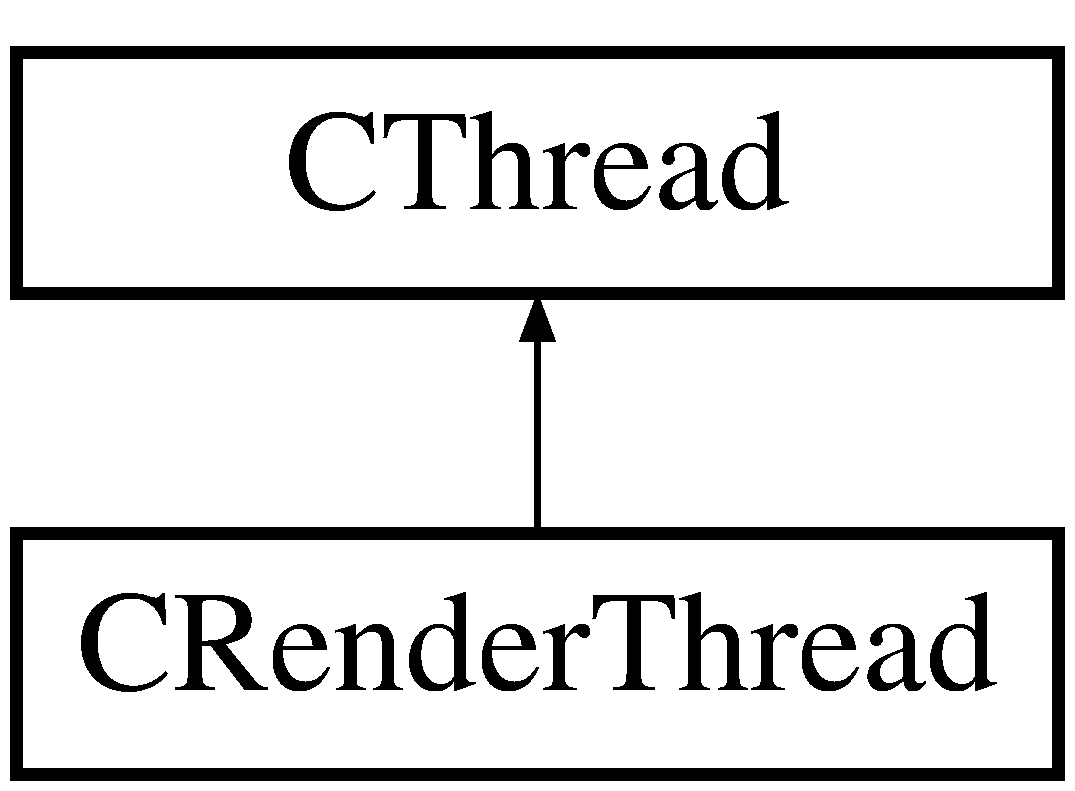
\includegraphics[height=2.000000cm]{class_c_render_thread}
\end{center}
\end{figure}
\subsection*{公開メンバ関数}
\begin{DoxyCompactItemize}
\item 
\hyperlink{class_c_render_thread_a2a679469847619c4525b60e9577aa70e}{C\+Render\+Thread} (\hyperlink{class_i_render_context}{I\+Render\+Context} $\ast$\+\_\+pc\+Render\+Context)
\begin{DoxyCompactList}\small\item\em コンストラクタ。 \end{DoxyCompactList}\item 
\hyperlink{class_c_render_thread_a7316ff44713f7951734875ef97fc0e64}{$\sim$\+C\+Render\+Thread} ()
\begin{DoxyCompactList}\small\item\em デストラクタ。 \end{DoxyCompactList}\item 
void \hyperlink{class_c_render_thread_a401df3e527ca4873e93d918ef10f0728}{Set\+Request\+Render} (bool \+\_\+b\+Request)
\begin{DoxyCompactList}\small\item\em 描画リクエスト。 \end{DoxyCompactList}\item 
bool \hyperlink{class_c_render_thread_a31a0dcd1c30f9366a53ea488444084d8}{Is\+Request\+Render} ()
\begin{DoxyCompactList}\small\item\em 描画リクエストがあるか。 \end{DoxyCompactList}\item 
void \hyperlink{class_c_render_thread_a17632fe814d63824d67c1ac96189dd6a}{Set\+Request\+End} (bool \+\_\+b\+End)
\begin{DoxyCompactList}\small\item\em 終了リクエスト。 \end{DoxyCompactList}\item 
bool \hyperlink{class_c_render_thread_abe60a79fc237ed4b620a11d3b35bdd66}{Is\+Request\+End} ()
\begin{DoxyCompactList}\small\item\em 終了リクエストがあるか。 \end{DoxyCompactList}\item 
\hyperlink{class_i_render_context}{I\+Render\+Context} $\ast$ \hyperlink{class_c_render_thread_aee6242ad8ffff36301faf978cb4065b7}{Get\+Render\+Context} ()
\begin{DoxyCompactList}\small\item\em 描画コンテキストを取得。 \end{DoxyCompactList}\item 
virtual void \hyperlink{class_c_render_thread_ac6c5c64b626dd62ad0d04e2a69db73ee}{Thread\+Callback} () final
\begin{DoxyCompactList}\small\item\em スレッドからコールバックされる関数。 \end{DoxyCompactList}\end{DoxyCompactItemize}
\subsection*{非公開変数類}
\begin{DoxyCompactItemize}
\item 
\hyperlink{class_i_render_context}{I\+Render\+Context} $\ast$ \hyperlink{class_c_render_thread_a781f8748290e6d59f8542b7f6b288815}{m\+\_\+pc\+Render\+Context}
\item 
bool \hyperlink{class_c_render_thread_a4684335c2982479e810c5e63ff07d246}{m\+\_\+b\+Request\+Render}
\item 
bool \hyperlink{class_c_render_thread_a47dc8a52ee3018731c821aad1505f54a}{m\+\_\+b\+Request\+End}
\item 
\hyperlink{class_c_critical_section}{C\+Critical\+Section} \hyperlink{class_c_render_thread_ab774ece4ffa6cd618cd02b888d9da06e}{m\+\_\+c\+Critical\+Section}
\end{DoxyCompactItemize}


\subsection{構築子と解体子}
\hypertarget{class_c_render_thread_a2a679469847619c4525b60e9577aa70e}{}\index{C\+Render\+Thread@{C\+Render\+Thread}!C\+Render\+Thread@{C\+Render\+Thread}}
\index{C\+Render\+Thread@{C\+Render\+Thread}!C\+Render\+Thread@{C\+Render\+Thread}}
\subsubsection[{C\+Render\+Thread(\+I\+Render\+Context $\ast$\+\_\+pc\+Render\+Context)}]{\setlength{\rightskip}{0pt plus 5cm}C\+Render\+Thread\+::\+C\+Render\+Thread (
\begin{DoxyParamCaption}
\item[{{\bf I\+Render\+Context} $\ast$}]{\+\_\+pc\+Render\+Context}
\end{DoxyParamCaption}
)}\label{class_c_render_thread_a2a679469847619c4525b60e9577aa70e}


コンストラクタ。 


\begin{DoxyParams}[1]{引数}
\mbox{\tt in}  & {\em \+\_\+pc\+Render\+Context} & \+: 描画コンテキスト。 \\
\hline
\end{DoxyParams}
\hypertarget{class_c_render_thread_a7316ff44713f7951734875ef97fc0e64}{}\index{C\+Render\+Thread@{C\+Render\+Thread}!````~C\+Render\+Thread@{$\sim$\+C\+Render\+Thread}}
\index{````~C\+Render\+Thread@{$\sim$\+C\+Render\+Thread}!C\+Render\+Thread@{C\+Render\+Thread}}
\subsubsection[{$\sim$\+C\+Render\+Thread()}]{\setlength{\rightskip}{0pt plus 5cm}C\+Render\+Thread\+::$\sim$\+C\+Render\+Thread (
\begin{DoxyParamCaption}
{}
\end{DoxyParamCaption}
)\hspace{0.3cm}{\ttfamily [inline]}}\label{class_c_render_thread_a7316ff44713f7951734875ef97fc0e64}


デストラクタ。 



\subsection{関数詳解}
\hypertarget{class_c_render_thread_aee6242ad8ffff36301faf978cb4065b7}{}\index{C\+Render\+Thread@{C\+Render\+Thread}!Get\+Render\+Context@{Get\+Render\+Context}}
\index{Get\+Render\+Context@{Get\+Render\+Context}!C\+Render\+Thread@{C\+Render\+Thread}}
\subsubsection[{Get\+Render\+Context()}]{\setlength{\rightskip}{0pt plus 5cm}{\bf I\+Render\+Context} $\ast$ C\+Render\+Thread\+::\+Get\+Render\+Context (
\begin{DoxyParamCaption}
{}
\end{DoxyParamCaption}
)}\label{class_c_render_thread_aee6242ad8ffff36301faf978cb4065b7}


描画コンテキストを取得。 


\begin{DoxyRetVals}{戻り値}
{\em \hyperlink{class_i_render_context}{I\+Render\+Context}} & \+: 描画コンテキスト。 \\
\hline
\end{DoxyRetVals}
\hypertarget{class_c_render_thread_abe60a79fc237ed4b620a11d3b35bdd66}{}\index{C\+Render\+Thread@{C\+Render\+Thread}!Is\+Request\+End@{Is\+Request\+End}}
\index{Is\+Request\+End@{Is\+Request\+End}!C\+Render\+Thread@{C\+Render\+Thread}}
\subsubsection[{Is\+Request\+End()}]{\setlength{\rightskip}{0pt plus 5cm}bool C\+Render\+Thread\+::\+Is\+Request\+End (
\begin{DoxyParamCaption}
{}
\end{DoxyParamCaption}
)}\label{class_c_render_thread_abe60a79fc237ed4b620a11d3b35bdd66}


終了リクエストがあるか。 


\begin{DoxyRetVals}{戻り値}
{\em bool} & \+: 終了リクエストがあればtrue。 \\
\hline
\end{DoxyRetVals}
\hypertarget{class_c_render_thread_a31a0dcd1c30f9366a53ea488444084d8}{}\index{C\+Render\+Thread@{C\+Render\+Thread}!Is\+Request\+Render@{Is\+Request\+Render}}
\index{Is\+Request\+Render@{Is\+Request\+Render}!C\+Render\+Thread@{C\+Render\+Thread}}
\subsubsection[{Is\+Request\+Render()}]{\setlength{\rightskip}{0pt plus 5cm}bool C\+Render\+Thread\+::\+Is\+Request\+Render (
\begin{DoxyParamCaption}
{}
\end{DoxyParamCaption}
)}\label{class_c_render_thread_a31a0dcd1c30f9366a53ea488444084d8}


描画リクエストがあるか。 


\begin{DoxyRetVals}{戻り値}
{\em bool} & \+: 描画リクエストがあればtrue。 \\
\hline
\end{DoxyRetVals}
\hypertarget{class_c_render_thread_a17632fe814d63824d67c1ac96189dd6a}{}\index{C\+Render\+Thread@{C\+Render\+Thread}!Set\+Request\+End@{Set\+Request\+End}}
\index{Set\+Request\+End@{Set\+Request\+End}!C\+Render\+Thread@{C\+Render\+Thread}}
\subsubsection[{Set\+Request\+End(bool \+\_\+b\+End)}]{\setlength{\rightskip}{0pt plus 5cm}void C\+Render\+Thread\+::\+Set\+Request\+End (
\begin{DoxyParamCaption}
\item[{bool}]{\+\_\+b\+Request}
\end{DoxyParamCaption}
)}\label{class_c_render_thread_a17632fe814d63824d67c1ac96189dd6a}


終了リクエスト。 


\begin{DoxyParams}[1]{引数}
\mbox{\tt in}  & {\em \+\_\+b\+Request} & \+: trueなら終了する。 \\
\hline
\end{DoxyParams}
\hypertarget{class_c_render_thread_a401df3e527ca4873e93d918ef10f0728}{}\index{C\+Render\+Thread@{C\+Render\+Thread}!Set\+Request\+Render@{Set\+Request\+Render}}
\index{Set\+Request\+Render@{Set\+Request\+Render}!C\+Render\+Thread@{C\+Render\+Thread}}
\subsubsection[{Set\+Request\+Render(bool \+\_\+b\+Request)}]{\setlength{\rightskip}{0pt plus 5cm}void C\+Render\+Thread\+::\+Set\+Request\+Render (
\begin{DoxyParamCaption}
\item[{bool}]{\+\_\+b\+Request}
\end{DoxyParamCaption}
)}\label{class_c_render_thread_a401df3e527ca4873e93d918ef10f0728}


描画リクエスト。 


\begin{DoxyParams}[1]{引数}
\mbox{\tt in}  & {\em \+\_\+b\+Request} & \+: trueならリクエストを行う。 \\
\hline
\end{DoxyParams}
\hypertarget{class_c_render_thread_ac6c5c64b626dd62ad0d04e2a69db73ee}{}\index{C\+Render\+Thread@{C\+Render\+Thread}!Thread\+Callback@{Thread\+Callback}}
\index{Thread\+Callback@{Thread\+Callback}!C\+Render\+Thread@{C\+Render\+Thread}}
\subsubsection[{Thread\+Callback() final}]{\setlength{\rightskip}{0pt plus 5cm}void C\+Render\+Thread\+::\+Thread\+Callback (
\begin{DoxyParamCaption}
{}
\end{DoxyParamCaption}
)\hspace{0.3cm}{\ttfamily [final]}, {\ttfamily [virtual]}}\label{class_c_render_thread_ac6c5c64b626dd62ad0d04e2a69db73ee}


スレッドからコールバックされる関数。 

ループ。 

\hyperlink{class_c_thread_a15c60ba6d652d92c150fda5e10ebb23e}{C\+Thread}を再実装しています。



\subsection{メンバ詳解}
\hypertarget{class_c_render_thread_a47dc8a52ee3018731c821aad1505f54a}{}\index{C\+Render\+Thread@{C\+Render\+Thread}!m\+\_\+b\+Request\+End@{m\+\_\+b\+Request\+End}}
\index{m\+\_\+b\+Request\+End@{m\+\_\+b\+Request\+End}!C\+Render\+Thread@{C\+Render\+Thread}}
\subsubsection[{m\+\_\+b\+Request\+End}]{\setlength{\rightskip}{0pt plus 5cm}bool C\+Render\+Thread\+::m\+\_\+b\+Request\+End\hspace{0.3cm}{\ttfamily [private]}}\label{class_c_render_thread_a47dc8a52ee3018731c821aad1505f54a}
\hypertarget{class_c_render_thread_a4684335c2982479e810c5e63ff07d246}{}\index{C\+Render\+Thread@{C\+Render\+Thread}!m\+\_\+b\+Request\+Render@{m\+\_\+b\+Request\+Render}}
\index{m\+\_\+b\+Request\+Render@{m\+\_\+b\+Request\+Render}!C\+Render\+Thread@{C\+Render\+Thread}}
\subsubsection[{m\+\_\+b\+Request\+Render}]{\setlength{\rightskip}{0pt plus 5cm}bool C\+Render\+Thread\+::m\+\_\+b\+Request\+Render\hspace{0.3cm}{\ttfamily [private]}}\label{class_c_render_thread_a4684335c2982479e810c5e63ff07d246}
\hypertarget{class_c_render_thread_ab774ece4ffa6cd618cd02b888d9da06e}{}\index{C\+Render\+Thread@{C\+Render\+Thread}!m\+\_\+c\+Critical\+Section@{m\+\_\+c\+Critical\+Section}}
\index{m\+\_\+c\+Critical\+Section@{m\+\_\+c\+Critical\+Section}!C\+Render\+Thread@{C\+Render\+Thread}}
\subsubsection[{m\+\_\+c\+Critical\+Section}]{\setlength{\rightskip}{0pt plus 5cm}{\bf C\+Critical\+Section} C\+Render\+Thread\+::m\+\_\+c\+Critical\+Section\hspace{0.3cm}{\ttfamily [private]}}\label{class_c_render_thread_ab774ece4ffa6cd618cd02b888d9da06e}
\hypertarget{class_c_render_thread_a781f8748290e6d59f8542b7f6b288815}{}\index{C\+Render\+Thread@{C\+Render\+Thread}!m\+\_\+pc\+Render\+Context@{m\+\_\+pc\+Render\+Context}}
\index{m\+\_\+pc\+Render\+Context@{m\+\_\+pc\+Render\+Context}!C\+Render\+Thread@{C\+Render\+Thread}}
\subsubsection[{m\+\_\+pc\+Render\+Context}]{\setlength{\rightskip}{0pt plus 5cm}{\bf I\+Render\+Context}$\ast$ C\+Render\+Thread\+::m\+\_\+pc\+Render\+Context\hspace{0.3cm}{\ttfamily [private]}}\label{class_c_render_thread_a781f8748290e6d59f8542b7f6b288815}


このクラス詳解は次のファイルから抽出されました\+:\begin{DoxyCompactItemize}
\item 
D\+:/\+Project/\+Game/\+Lib/\+Render/\hyperlink{_render_thread_8h}{Render\+Thread.\+h}\item 
D\+:/\+Project/\+Game/\+Lib/\+Render/\hyperlink{_render_thread_8cpp}{Render\+Thread.\+cpp}\end{DoxyCompactItemize}

\hypertarget{class_c_sequence}{}\section{C\+Sequence クラス}
\label{class_c_sequence}\index{C\+Sequence@{C\+Sequence}}


{\ttfamily \#include $<$Sequence.\+h$>$}

C\+Sequence の継承関係図\begin{figure}[H]
\begin{center}
\leavevmode
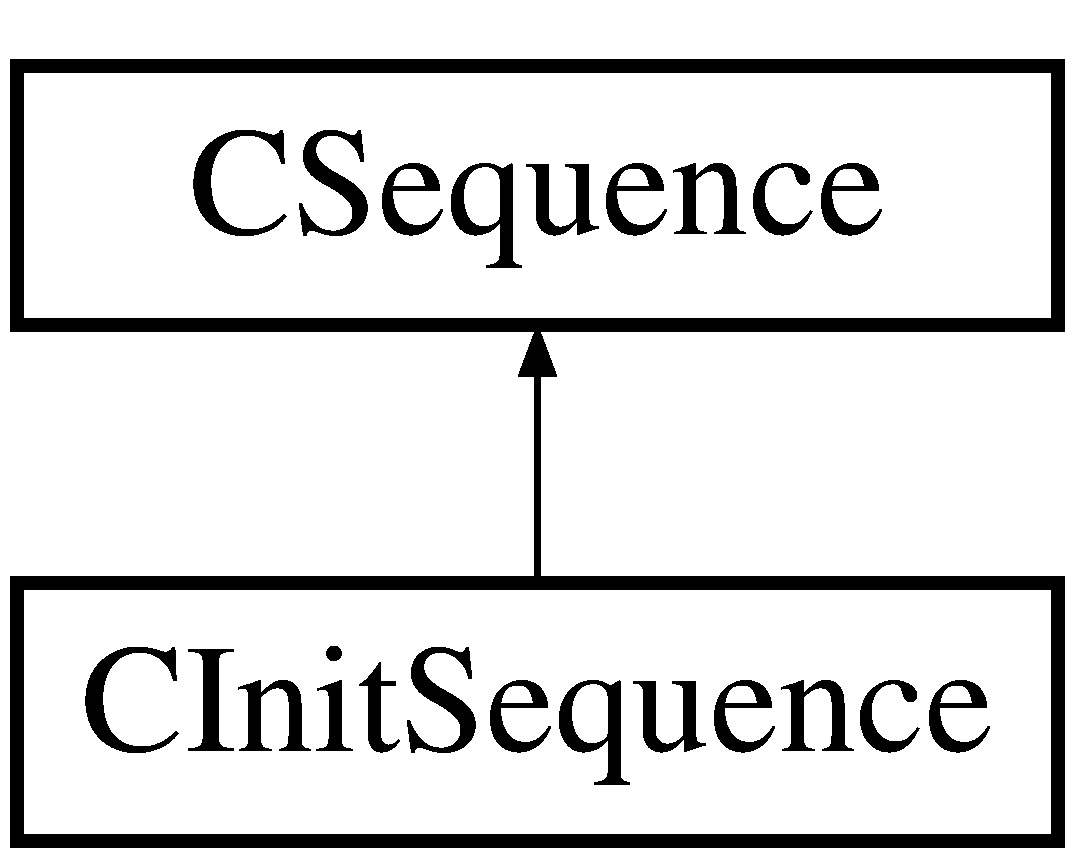
\includegraphics[height=2.000000cm]{class_c_sequence}
\end{center}
\end{figure}
\subsection*{公開メンバ関数}
\begin{DoxyCompactItemize}
\item 
\hyperlink{class_c_sequence_a6cc3de702f301236a8a37a87ed725a67}{C\+Sequence} ()
\begin{DoxyCompactList}\small\item\em コンストラクタ。 \end{DoxyCompactList}\item 
virtual \hyperlink{class_c_sequence_ab3f7e5cb5fb63272423e0b5075189d62}{$\sim$\+C\+Sequence} ()
\begin{DoxyCompactList}\small\item\em デストラクタ。 \end{DoxyCompactList}\item 
virtual void \hyperlink{class_c_sequence_a0124977c5ae40f9289c7867ff71c743d}{Loop\+Start\+Act} ()
\begin{DoxyCompactList}\small\item\em フレーム開始時に行う処理。 \end{DoxyCompactList}\item 
virtual void \hyperlink{class_c_sequence_a0a2f5146bf33a4bd8c480d9da5a0538d}{Loop\+End\+Act} ()
\begin{DoxyCompactList}\small\item\em フレーム終了時に行う処理。 \end{DoxyCompactList}\item 
virtual bool \hyperlink{class_c_sequence_acec92faef8ee677063980776b4c242a1}{Is\+End} () const  =0
\begin{DoxyCompactList}\small\item\em シーケンスが終了したか。 \end{DoxyCompactList}\item 
virtual U32 \hyperlink{class_c_sequence_a9819cf065c49e5a8bee7f04f62d37d16}{Get\+Next} () const  =0
\begin{DoxyCompactList}\small\item\em 次のシーケンスを取得。 \end{DoxyCompactList}\end{DoxyCompactItemize}


\subsection{構築子と解体子}
\hypertarget{class_c_sequence_a6cc3de702f301236a8a37a87ed725a67}{}\index{C\+Sequence@{C\+Sequence}!C\+Sequence@{C\+Sequence}}
\index{C\+Sequence@{C\+Sequence}!C\+Sequence@{C\+Sequence}}
\subsubsection[{C\+Sequence()}]{\setlength{\rightskip}{0pt plus 5cm}C\+Sequence\+::\+C\+Sequence (
\begin{DoxyParamCaption}
{}
\end{DoxyParamCaption}
)\hspace{0.3cm}{\ttfamily [inline]}}\label{class_c_sequence_a6cc3de702f301236a8a37a87ed725a67}


コンストラクタ。 

\hypertarget{class_c_sequence_ab3f7e5cb5fb63272423e0b5075189d62}{}\index{C\+Sequence@{C\+Sequence}!````~C\+Sequence@{$\sim$\+C\+Sequence}}
\index{````~C\+Sequence@{$\sim$\+C\+Sequence}!C\+Sequence@{C\+Sequence}}
\subsubsection[{$\sim$\+C\+Sequence()}]{\setlength{\rightskip}{0pt plus 5cm}virtual C\+Sequence\+::$\sim$\+C\+Sequence (
\begin{DoxyParamCaption}
{}
\end{DoxyParamCaption}
)\hspace{0.3cm}{\ttfamily [inline]}, {\ttfamily [virtual]}}\label{class_c_sequence_ab3f7e5cb5fb63272423e0b5075189d62}


デストラクタ。 



\subsection{関数詳解}
\hypertarget{class_c_sequence_a9819cf065c49e5a8bee7f04f62d37d16}{}\index{C\+Sequence@{C\+Sequence}!Get\+Next@{Get\+Next}}
\index{Get\+Next@{Get\+Next}!C\+Sequence@{C\+Sequence}}
\subsubsection[{Get\+Next() const  =0}]{\setlength{\rightskip}{0pt plus 5cm}virtual U32 C\+Sequence\+::\+Get\+Next (
\begin{DoxyParamCaption}
{}
\end{DoxyParamCaption}
) const\hspace{0.3cm}{\ttfamily [pure virtual]}}\label{class_c_sequence_a9819cf065c49e5a8bee7f04f62d37d16}


次のシーケンスを取得。 



\hyperlink{class_c_init_sequence_a7d4aec0184771958424f2234716a4945}{C\+Init\+Sequence}で実装されています。

\hypertarget{class_c_sequence_acec92faef8ee677063980776b4c242a1}{}\index{C\+Sequence@{C\+Sequence}!Is\+End@{Is\+End}}
\index{Is\+End@{Is\+End}!C\+Sequence@{C\+Sequence}}
\subsubsection[{Is\+End() const  =0}]{\setlength{\rightskip}{0pt plus 5cm}virtual bool C\+Sequence\+::\+Is\+End (
\begin{DoxyParamCaption}
{}
\end{DoxyParamCaption}
) const\hspace{0.3cm}{\ttfamily [pure virtual]}}\label{class_c_sequence_acec92faef8ee677063980776b4c242a1}


シーケンスが終了したか。 



\hyperlink{class_c_init_sequence_ac837c22aeab7e9c10f3f9a217390661c}{C\+Init\+Sequence}で実装されています。

\hypertarget{class_c_sequence_a0a2f5146bf33a4bd8c480d9da5a0538d}{}\index{C\+Sequence@{C\+Sequence}!Loop\+End\+Act@{Loop\+End\+Act}}
\index{Loop\+End\+Act@{Loop\+End\+Act}!C\+Sequence@{C\+Sequence}}
\subsubsection[{Loop\+End\+Act()}]{\setlength{\rightskip}{0pt plus 5cm}virtual void C\+Sequence\+::\+Loop\+End\+Act (
\begin{DoxyParamCaption}
{}
\end{DoxyParamCaption}
)\hspace{0.3cm}{\ttfamily [inline]}, {\ttfamily [virtual]}}\label{class_c_sequence_a0a2f5146bf33a4bd8c480d9da5a0538d}


フレーム終了時に行う処理。 



\hyperlink{class_c_init_sequence_aae10f421cc1738b571022d2bdc3898d0}{C\+Init\+Sequence}で再実装されています。

\hypertarget{class_c_sequence_a0124977c5ae40f9289c7867ff71c743d}{}\index{C\+Sequence@{C\+Sequence}!Loop\+Start\+Act@{Loop\+Start\+Act}}
\index{Loop\+Start\+Act@{Loop\+Start\+Act}!C\+Sequence@{C\+Sequence}}
\subsubsection[{Loop\+Start\+Act()}]{\setlength{\rightskip}{0pt plus 5cm}virtual void C\+Sequence\+::\+Loop\+Start\+Act (
\begin{DoxyParamCaption}
{}
\end{DoxyParamCaption}
)\hspace{0.3cm}{\ttfamily [inline]}, {\ttfamily [virtual]}}\label{class_c_sequence_a0124977c5ae40f9289c7867ff71c743d}


フレーム開始時に行う処理。 



\hyperlink{class_c_init_sequence_a52cb5822b6f2c281f3969fadc61a47fb}{C\+Init\+Sequence}で再実装されています。



このクラス詳解は次のファイルから抽出されました\+:\begin{DoxyCompactItemize}
\item 
D\+:/\+Project/\+Game/\+Lib/\+Sequence/\hyperlink{_sequence_8h}{Sequence.\+h}\end{DoxyCompactItemize}

\hypertarget{class_c_sequence_control}{}\section{C\+Sequence\+Control クラス}
\label{class_c_sequence_control}\index{C\+Sequence\+Control@{C\+Sequence\+Control}}


{\ttfamily \#include $<$Sequence\+Control.\+h$>$}

\subsection*{クラス}
\begin{DoxyCompactItemize}
\item 
struct \hyperlink{struct_c_sequence_control_1_1_st_init_param}{St\+Init\+Param}
\begin{DoxyCompactList}\small\item\em 初期化用パラメータ。 \end{DoxyCompactList}\end{DoxyCompactItemize}
\subsection*{公開メンバ関数}
\begin{DoxyCompactItemize}
\item 
\hyperlink{class_c_sequence_control_ad011ae31839cf8cc69d292bf16cf231d}{C\+Sequence\+Control} (const \hyperlink{struct_c_sequence_control_1_1_st_init_param}{St\+Init\+Param} \&\+\_\+rst\+Init\+Param)
\begin{DoxyCompactList}\small\item\em コンストラクタ。 \end{DoxyCompactList}\item 
virtual \hyperlink{class_c_sequence_control_a8735abbbdd83d4ef744ffb29fee7a450}{$\sim$\+C\+Sequence\+Control} ()
\begin{DoxyCompactList}\small\item\em デストラクタ。 \end{DoxyCompactList}\item 
void \hyperlink{class_c_sequence_control_ad4eb050fd932a4e69a1a7872342da3b2}{Loop\+Start\+Act} ()
\begin{DoxyCompactList}\small\item\em フレーム開始時の処理。 \end{DoxyCompactList}\item 
void \hyperlink{class_c_sequence_control_a42709cbc26a634d5e917587d581f9266}{Loop\+End\+Act} ()
\begin{DoxyCompactList}\small\item\em フレーム終了時の処理。 \end{DoxyCompactList}\end{DoxyCompactItemize}
\subsection*{非公開変数類}
\begin{DoxyCompactItemize}
\item 
\hyperlink{class_c_sequence}{C\+Sequence} $\ast$ \hyperlink{class_c_sequence_control_af3d3db5891e39a284d94ec49c34a153d}{m\+\_\+pc\+Sequence}
\item 
\hyperlink{class_c_sequence_factory}{C\+Sequence\+Factory} $\ast$ \hyperlink{class_c_sequence_control_acbb8764a37066e4f3e5bc02a88fc17b2}{m\+\_\+pc\+Factory}
\end{DoxyCompactItemize}


\subsection{構築子と解体子}
\hypertarget{class_c_sequence_control_ad011ae31839cf8cc69d292bf16cf231d}{}\index{C\+Sequence\+Control@{C\+Sequence\+Control}!C\+Sequence\+Control@{C\+Sequence\+Control}}
\index{C\+Sequence\+Control@{C\+Sequence\+Control}!C\+Sequence\+Control@{C\+Sequence\+Control}}
\subsubsection[{C\+Sequence\+Control(const St\+Init\+Param \&\+\_\+rst\+Init\+Param)}]{\setlength{\rightskip}{0pt plus 5cm}C\+Sequence\+Control\+::\+C\+Sequence\+Control (
\begin{DoxyParamCaption}
\item[{const {\bf St\+Init\+Param} \&}]{\+\_\+rst\+Init\+Param}
\end{DoxyParamCaption}
)}\label{class_c_sequence_control_ad011ae31839cf8cc69d292bf16cf231d}


コンストラクタ。 


\begin{DoxyParams}{引数}
{\em \+\_\+rst\+Init\+Param} & \+: 初期化用パラメータ。 \\
\hline
\end{DoxyParams}
\hypertarget{class_c_sequence_control_a8735abbbdd83d4ef744ffb29fee7a450}{}\index{C\+Sequence\+Control@{C\+Sequence\+Control}!````~C\+Sequence\+Control@{$\sim$\+C\+Sequence\+Control}}
\index{````~C\+Sequence\+Control@{$\sim$\+C\+Sequence\+Control}!C\+Sequence\+Control@{C\+Sequence\+Control}}
\subsubsection[{$\sim$\+C\+Sequence\+Control()}]{\setlength{\rightskip}{0pt plus 5cm}C\+Sequence\+Control\+::$\sim$\+C\+Sequence\+Control (
\begin{DoxyParamCaption}
{}
\end{DoxyParamCaption}
)\hspace{0.3cm}{\ttfamily [virtual]}}\label{class_c_sequence_control_a8735abbbdd83d4ef744ffb29fee7a450}


デストラクタ。 



\subsection{関数詳解}
\hypertarget{class_c_sequence_control_a42709cbc26a634d5e917587d581f9266}{}\index{C\+Sequence\+Control@{C\+Sequence\+Control}!Loop\+End\+Act@{Loop\+End\+Act}}
\index{Loop\+End\+Act@{Loop\+End\+Act}!C\+Sequence\+Control@{C\+Sequence\+Control}}
\subsubsection[{Loop\+End\+Act()}]{\setlength{\rightskip}{0pt plus 5cm}void C\+Sequence\+Control\+::\+Loop\+End\+Act (
\begin{DoxyParamCaption}
{}
\end{DoxyParamCaption}
)}\label{class_c_sequence_control_a42709cbc26a634d5e917587d581f9266}


フレーム終了時の処理。 

\hypertarget{class_c_sequence_control_ad4eb050fd932a4e69a1a7872342da3b2}{}\index{C\+Sequence\+Control@{C\+Sequence\+Control}!Loop\+Start\+Act@{Loop\+Start\+Act}}
\index{Loop\+Start\+Act@{Loop\+Start\+Act}!C\+Sequence\+Control@{C\+Sequence\+Control}}
\subsubsection[{Loop\+Start\+Act()}]{\setlength{\rightskip}{0pt plus 5cm}void C\+Sequence\+Control\+::\+Loop\+Start\+Act (
\begin{DoxyParamCaption}
{}
\end{DoxyParamCaption}
)}\label{class_c_sequence_control_ad4eb050fd932a4e69a1a7872342da3b2}


フレーム開始時の処理。 

フレーム開始時の処理 

\subsection{メンバ詳解}
\hypertarget{class_c_sequence_control_acbb8764a37066e4f3e5bc02a88fc17b2}{}\index{C\+Sequence\+Control@{C\+Sequence\+Control}!m\+\_\+pc\+Factory@{m\+\_\+pc\+Factory}}
\index{m\+\_\+pc\+Factory@{m\+\_\+pc\+Factory}!C\+Sequence\+Control@{C\+Sequence\+Control}}
\subsubsection[{m\+\_\+pc\+Factory}]{\setlength{\rightskip}{0pt plus 5cm}{\bf C\+Sequence\+Factory}$\ast$ C\+Sequence\+Control\+::m\+\_\+pc\+Factory\hspace{0.3cm}{\ttfamily [private]}}\label{class_c_sequence_control_acbb8764a37066e4f3e5bc02a88fc17b2}
\hypertarget{class_c_sequence_control_af3d3db5891e39a284d94ec49c34a153d}{}\index{C\+Sequence\+Control@{C\+Sequence\+Control}!m\+\_\+pc\+Sequence@{m\+\_\+pc\+Sequence}}
\index{m\+\_\+pc\+Sequence@{m\+\_\+pc\+Sequence}!C\+Sequence\+Control@{C\+Sequence\+Control}}
\subsubsection[{m\+\_\+pc\+Sequence}]{\setlength{\rightskip}{0pt plus 5cm}{\bf C\+Sequence}$\ast$ C\+Sequence\+Control\+::m\+\_\+pc\+Sequence\hspace{0.3cm}{\ttfamily [private]}}\label{class_c_sequence_control_af3d3db5891e39a284d94ec49c34a153d}


このクラス詳解は次のファイルから抽出されました\+:\begin{DoxyCompactItemize}
\item 
D\+:/\+Project/\+Game/\+Lib/\+Sequence/\hyperlink{_sequence_control_8h}{Sequence\+Control.\+h}\item 
D\+:/\+Project/\+Game/\+Lib/\+Sequence/\hyperlink{_sequence_control_8cpp}{Sequence\+Control.\+cpp}\end{DoxyCompactItemize}

\hypertarget{class_c_sequence_factory}{}\section{C\+Sequence\+Factory クラス}
\label{class_c_sequence_factory}\index{C\+Sequence\+Factory@{C\+Sequence\+Factory}}


{\ttfamily \#include $<$Sequence\+Factory.\+h$>$}

C\+Sequence\+Factory の継承関係図\begin{figure}[H]
\begin{center}
\leavevmode
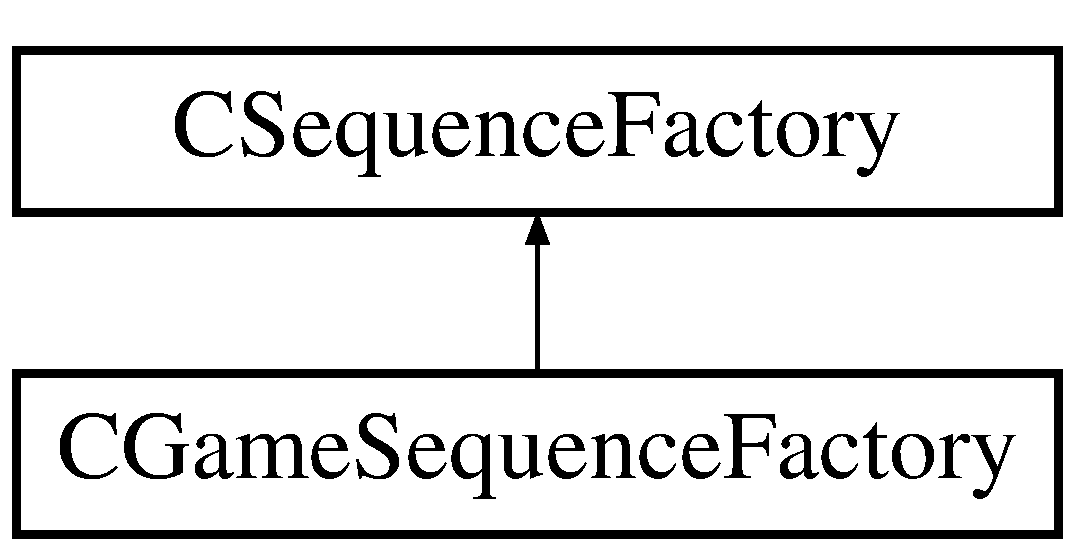
\includegraphics[height=2.000000cm]{class_c_sequence_factory}
\end{center}
\end{figure}
\subsection*{公開メンバ関数}
\begin{DoxyCompactItemize}
\item 
\hyperlink{class_c_sequence_factory_a45431bbc767b1232b42c06ce3ea88c1a}{C\+Sequence\+Factory} ()
\begin{DoxyCompactList}\small\item\em コンストラクタ。 \end{DoxyCompactList}\item 
virtual \hyperlink{class_c_sequence_factory_a62f30b0db6ff02fa8d535550d910bfda}{$\sim$\+C\+Sequence\+Factory} ()
\begin{DoxyCompactList}\small\item\em デストラクタ。 \end{DoxyCompactList}\item 
virtual \hyperlink{class_c_sequence}{C\+Sequence} $\ast$ \hyperlink{class_c_sequence_factory_aba3a273d0da93264b7d18e43d86d4c39}{Create\+Instance} (U32 \+\_\+u\+Sequence\+I\+D)
\begin{DoxyCompactList}\small\item\em シーケンスのインスタンス生成。 \end{DoxyCompactList}\end{DoxyCompactItemize}


\subsection{構築子と解体子}
\hypertarget{class_c_sequence_factory_a45431bbc767b1232b42c06ce3ea88c1a}{}\index{C\+Sequence\+Factory@{C\+Sequence\+Factory}!C\+Sequence\+Factory@{C\+Sequence\+Factory}}
\index{C\+Sequence\+Factory@{C\+Sequence\+Factory}!C\+Sequence\+Factory@{C\+Sequence\+Factory}}
\subsubsection[{C\+Sequence\+Factory()}]{\setlength{\rightskip}{0pt plus 5cm}C\+Sequence\+Factory\+::\+C\+Sequence\+Factory (
\begin{DoxyParamCaption}
{}
\end{DoxyParamCaption}
)\hspace{0.3cm}{\ttfamily [inline]}}\label{class_c_sequence_factory_a45431bbc767b1232b42c06ce3ea88c1a}


コンストラクタ。 

\hypertarget{class_c_sequence_factory_a62f30b0db6ff02fa8d535550d910bfda}{}\index{C\+Sequence\+Factory@{C\+Sequence\+Factory}!````~C\+Sequence\+Factory@{$\sim$\+C\+Sequence\+Factory}}
\index{````~C\+Sequence\+Factory@{$\sim$\+C\+Sequence\+Factory}!C\+Sequence\+Factory@{C\+Sequence\+Factory}}
\subsubsection[{$\sim$\+C\+Sequence\+Factory()}]{\setlength{\rightskip}{0pt plus 5cm}virtual C\+Sequence\+Factory\+::$\sim$\+C\+Sequence\+Factory (
\begin{DoxyParamCaption}
{}
\end{DoxyParamCaption}
)\hspace{0.3cm}{\ttfamily [inline]}, {\ttfamily [virtual]}}\label{class_c_sequence_factory_a62f30b0db6ff02fa8d535550d910bfda}


デストラクタ。 



\subsection{関数詳解}
\hypertarget{class_c_sequence_factory_aba3a273d0da93264b7d18e43d86d4c39}{}\index{C\+Sequence\+Factory@{C\+Sequence\+Factory}!Create\+Instance@{Create\+Instance}}
\index{Create\+Instance@{Create\+Instance}!C\+Sequence\+Factory@{C\+Sequence\+Factory}}
\subsubsection[{Create\+Instance(\+U32 \+\_\+u\+Sequence\+I\+D)}]{\setlength{\rightskip}{0pt plus 5cm}virtual {\bf C\+Sequence}$\ast$ C\+Sequence\+Factory\+::\+Create\+Instance (
\begin{DoxyParamCaption}
\item[{U32}]{\+\_\+u\+Sequence\+I\+D}
\end{DoxyParamCaption}
)\hspace{0.3cm}{\ttfamily [inline]}, {\ttfamily [virtual]}}\label{class_c_sequence_factory_aba3a273d0da93264b7d18e43d86d4c39}


シーケンスのインスタンス生成。 



\hyperlink{class_c_game_sequence_factory_a868862261fd54f2d6f05a7fd0ba41b34}{C\+Game\+Sequence\+Factory}で再実装されています。



このクラス詳解は次のファイルから抽出されました\+:\begin{DoxyCompactItemize}
\item 
D\+:/\+Project/\+Game/\+Lib/\+Sequence/\hyperlink{_sequence_factory_8h}{Sequence\+Factory.\+h}\end{DoxyCompactItemize}

\hypertarget{class_c_singleton}{}\section{C\+Singleton$<$ T $>$ クラステンプレート}
\label{class_c_singleton}\index{C\+Singleton$<$ T $>$@{C\+Singleton$<$ T $>$}}


{\ttfamily \#include $<$Singleton.\+h$>$}

\subsection*{静的公開メンバ関数}
\begin{DoxyCompactItemize}
\item 
static void \hyperlink{class_c_singleton_aae03d09669f6d715c19305e374caf447}{Create\+Instance} ()
\item 
static T $\ast$ \hyperlink{class_c_singleton_adca13e4aead62014a099f8377d2d0daf}{Get\+Instance} ()
\item 
static void \hyperlink{class_c_singleton_a40ab50a27926e8ae1efb62c793d3a425}{Destroy\+Instance} ()
\end{DoxyCompactItemize}
\subsection*{限定公開メンバ関数}
\begin{DoxyCompactItemize}
\item 
\hyperlink{class_c_singleton_a9363c7dab54cf622af286b1732a323a2}{C\+Singleton} ()
\begin{DoxyCompactList}\small\item\em コンストラクタ。 \end{DoxyCompactList}\item 
virtual \hyperlink{class_c_singleton_ab8ec20bd0d6d35ba4ab8987c2cd1bd09}{$\sim$\+C\+Singleton} ()
\begin{DoxyCompactList}\small\item\em デストラクタ。 \end{DoxyCompactList}\end{DoxyCompactItemize}
\subsection*{静的限定公開変数類}
\begin{DoxyCompactItemize}
\item 
static T $\ast$ \hyperlink{class_c_singleton_a0a71a6912e89df78d7f0fc5a79ff6d98}{sc\+\_\+pc\+Instance} = nullptr
\end{DoxyCompactItemize}
\subsection*{非公開メンバ関数}
\begin{DoxyCompactItemize}
\item 
\hyperlink{class_c_singleton_a83e4739133812fa496b4c619d899f361}{C\+Singleton} (const \hyperlink{class_c_singleton}{C\+Singleton} \&\+\_\+rc\+Ref)
\item 
\hyperlink{class_c_singleton}{C\+Singleton} \& \hyperlink{class_c_singleton_a549299f15a4d639c3ca069dc8c2e63f7}{operator=} (const \hyperlink{class_c_singleton}{C\+Singleton} \&\+\_\+rc\+Ref)
\begin{DoxyCompactList}\small\item\em 代入演算子。 \end{DoxyCompactList}\end{DoxyCompactItemize}


\subsection{構築子と解体子}
\hypertarget{class_c_singleton_a9363c7dab54cf622af286b1732a323a2}{}\index{C\+Singleton@{C\+Singleton}!C\+Singleton@{C\+Singleton}}
\index{C\+Singleton@{C\+Singleton}!C\+Singleton@{C\+Singleton}}
\subsubsection[{C\+Singleton()}]{\setlength{\rightskip}{0pt plus 5cm}template$<$class T$>$ {\bf C\+Singleton}$<$ T $>$\+::{\bf C\+Singleton} (
\begin{DoxyParamCaption}
{}
\end{DoxyParamCaption}
)\hspace{0.3cm}{\ttfamily [inline]}, {\ttfamily [protected]}}\label{class_c_singleton_a9363c7dab54cf622af286b1732a323a2}


コンストラクタ。 

\hypertarget{class_c_singleton_ab8ec20bd0d6d35ba4ab8987c2cd1bd09}{}\index{C\+Singleton@{C\+Singleton}!````~C\+Singleton@{$\sim$\+C\+Singleton}}
\index{````~C\+Singleton@{$\sim$\+C\+Singleton}!C\+Singleton@{C\+Singleton}}
\subsubsection[{$\sim$\+C\+Singleton()}]{\setlength{\rightskip}{0pt plus 5cm}template$<$class T$>$ virtual {\bf C\+Singleton}$<$ T $>$\+::$\sim${\bf C\+Singleton} (
\begin{DoxyParamCaption}
{}
\end{DoxyParamCaption}
)\hspace{0.3cm}{\ttfamily [inline]}, {\ttfamily [protected]}, {\ttfamily [virtual]}}\label{class_c_singleton_ab8ec20bd0d6d35ba4ab8987c2cd1bd09}


デストラクタ。 

\hypertarget{class_c_singleton_a83e4739133812fa496b4c619d899f361}{}\index{C\+Singleton@{C\+Singleton}!C\+Singleton@{C\+Singleton}}
\index{C\+Singleton@{C\+Singleton}!C\+Singleton@{C\+Singleton}}
\subsubsection[{C\+Singleton(const C\+Singleton \&\+\_\+rc\+Ref)}]{\setlength{\rightskip}{0pt plus 5cm}template$<$class T$>$ {\bf C\+Singleton}$<$ T $>$\+::{\bf C\+Singleton} (
\begin{DoxyParamCaption}
\item[{const {\bf C\+Singleton}$<$ T $>$ \&}]{\+\_\+rc\+Ref}
\end{DoxyParamCaption}
)\hspace{0.3cm}{\ttfamily [inline]}, {\ttfamily [private]}}\label{class_c_singleton_a83e4739133812fa496b4c619d899f361}
外部からの呼び出しを禁止する。 コピーコンストラクタ。 

\subsection{関数詳解}
\hypertarget{class_c_singleton_aae03d09669f6d715c19305e374caf447}{}\index{C\+Singleton@{C\+Singleton}!Create\+Instance@{Create\+Instance}}
\index{Create\+Instance@{Create\+Instance}!C\+Singleton@{C\+Singleton}}
\subsubsection[{Create\+Instance()}]{\setlength{\rightskip}{0pt plus 5cm}template$<$class T$>$ static void {\bf C\+Singleton}$<$ T $>$\+::Create\+Instance (
\begin{DoxyParamCaption}
{}
\end{DoxyParamCaption}
)\hspace{0.3cm}{\ttfamily [inline]}, {\ttfamily [static]}}\label{class_c_singleton_aae03d09669f6d715c19305e374caf447}
\hypertarget{class_c_singleton_a40ab50a27926e8ae1efb62c793d3a425}{}\index{C\+Singleton@{C\+Singleton}!Destroy\+Instance@{Destroy\+Instance}}
\index{Destroy\+Instance@{Destroy\+Instance}!C\+Singleton@{C\+Singleton}}
\subsubsection[{Destroy\+Instance()}]{\setlength{\rightskip}{0pt plus 5cm}template$<$class T$>$ static void {\bf C\+Singleton}$<$ T $>$\+::Destroy\+Instance (
\begin{DoxyParamCaption}
{}
\end{DoxyParamCaption}
)\hspace{0.3cm}{\ttfamily [inline]}, {\ttfamily [static]}}\label{class_c_singleton_a40ab50a27926e8ae1efb62c793d3a425}
\hypertarget{class_c_singleton_adca13e4aead62014a099f8377d2d0daf}{}\index{C\+Singleton@{C\+Singleton}!Get\+Instance@{Get\+Instance}}
\index{Get\+Instance@{Get\+Instance}!C\+Singleton@{C\+Singleton}}
\subsubsection[{Get\+Instance()}]{\setlength{\rightskip}{0pt plus 5cm}template$<$class T$>$ static T$\ast$ {\bf C\+Singleton}$<$ T $>$\+::Get\+Instance (
\begin{DoxyParamCaption}
{}
\end{DoxyParamCaption}
)\hspace{0.3cm}{\ttfamily [inline]}, {\ttfamily [static]}}\label{class_c_singleton_adca13e4aead62014a099f8377d2d0daf}
\hypertarget{class_c_singleton_a549299f15a4d639c3ca069dc8c2e63f7}{}\index{C\+Singleton@{C\+Singleton}!operator=@{operator=}}
\index{operator=@{operator=}!C\+Singleton@{C\+Singleton}}
\subsubsection[{operator=(const C\+Singleton \&\+\_\+rc\+Ref)}]{\setlength{\rightskip}{0pt plus 5cm}template$<$class T$>$ {\bf C\+Singleton}\& {\bf C\+Singleton}$<$ T $>$\+::operator= (
\begin{DoxyParamCaption}
\item[{const {\bf C\+Singleton}$<$ T $>$ \&}]{\+\_\+rc\+Ref}
\end{DoxyParamCaption}
)\hspace{0.3cm}{\ttfamily [inline]}, {\ttfamily [private]}}\label{class_c_singleton_a549299f15a4d639c3ca069dc8c2e63f7}


代入演算子。 



\subsection{メンバ詳解}
\hypertarget{class_c_singleton_a0a71a6912e89df78d7f0fc5a79ff6d98}{}\index{C\+Singleton@{C\+Singleton}!sc\+\_\+pc\+Instance@{sc\+\_\+pc\+Instance}}
\index{sc\+\_\+pc\+Instance@{sc\+\_\+pc\+Instance}!C\+Singleton@{C\+Singleton}}
\subsubsection[{sc\+\_\+pc\+Instance}]{\setlength{\rightskip}{0pt plus 5cm}template$<$class T$>$ T $\ast$ {\bf C\+Singleton}$<$ T $>$\+::sc\+\_\+pc\+Instance = nullptr\hspace{0.3cm}{\ttfamily [static]}, {\ttfamily [protected]}}\label{class_c_singleton_a0a71a6912e89df78d7f0fc5a79ff6d98}


このクラス詳解は次のファイルから抽出されました\+:\begin{DoxyCompactItemize}
\item 
D\+:/\+Project/\+Game/\+Lib/\+Utility/\hyperlink{_singleton_8h}{Singleton.\+h}\end{DoxyCompactItemize}

\hypertarget{class_c_thread}{}\section{C\+Thread クラス}
\label{class_c_thread}\index{C\+Thread@{C\+Thread}}


{\ttfamily \#include $<$Thread.\+h$>$}

C\+Thread の継承関係図\begin{figure}[H]
\begin{center}
\leavevmode
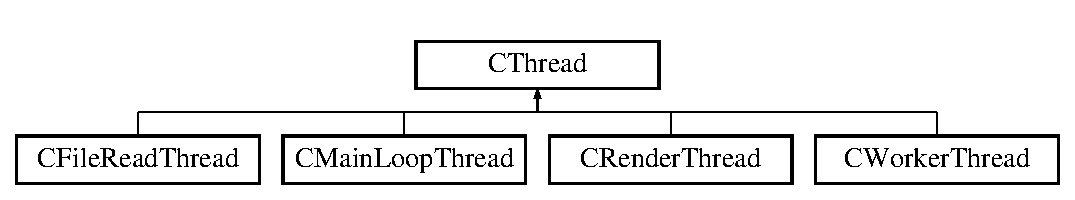
\includegraphics[height=2.000000cm]{class_c_thread}
\end{center}
\end{figure}
\subsection*{公開メンバ関数}
\begin{DoxyCompactItemize}
\item 
\hyperlink{class_c_thread_ad256868eded3b90abee1b5f656bb678e}{C\+Thread} ()
\begin{DoxyCompactList}\small\item\em コンストラクタ。 \end{DoxyCompactList}\item 
virtual \hyperlink{class_c_thread_a85a583b2edf56a6448e71e3a9ad301d2}{$\sim$\+C\+Thread} ()
\begin{DoxyCompactList}\small\item\em デストラクタ。 \end{DoxyCompactList}\item 
void \hyperlink{class_c_thread_afa189114d2d65ea7e39679d1ecc6466d}{Run} ()
\begin{DoxyCompactList}\small\item\em スレッド開始。 \end{DoxyCompactList}\item 
void \hyperlink{class_c_thread_a149db91da8c8672ef841a9136c8fae43}{Wait\+End} ()
\begin{DoxyCompactList}\small\item\em スレッドの終了待ち。 \end{DoxyCompactList}\item 
virtual void \hyperlink{class_c_thread_a15c60ba6d652d92c150fda5e10ebb23e}{Thread\+Callback} ()
\begin{DoxyCompactList}\small\item\em 開始したスレッドから呼ばれるコールバック関数。 \end{DoxyCompactList}\end{DoxyCompactItemize}
\subsection*{非公開変数類}
\begin{DoxyCompactItemize}
\item 
std\+::thread \hyperlink{class_c_thread_ae9a1eb632950ffb7a12228ab7c8b9ade}{m\+\_\+c\+Thread}
\item 
bool \hyperlink{class_c_thread_a6c06ca19f97664620c40a1807f99159f}{m\+\_\+b\+Start\+Thread}
\end{DoxyCompactItemize}


\subsection{構築子と解体子}
\hypertarget{class_c_thread_ad256868eded3b90abee1b5f656bb678e}{}\index{C\+Thread@{C\+Thread}!C\+Thread@{C\+Thread}}
\index{C\+Thread@{C\+Thread}!C\+Thread@{C\+Thread}}
\subsubsection[{C\+Thread()}]{\setlength{\rightskip}{0pt plus 5cm}C\+Thread\+::\+C\+Thread (
\begin{DoxyParamCaption}
{}
\end{DoxyParamCaption}
)}\label{class_c_thread_ad256868eded3b90abee1b5f656bb678e}


コンストラクタ。 

\hypertarget{class_c_thread_a85a583b2edf56a6448e71e3a9ad301d2}{}\index{C\+Thread@{C\+Thread}!````~C\+Thread@{$\sim$\+C\+Thread}}
\index{````~C\+Thread@{$\sim$\+C\+Thread}!C\+Thread@{C\+Thread}}
\subsubsection[{$\sim$\+C\+Thread()}]{\setlength{\rightskip}{0pt plus 5cm}C\+Thread\+::$\sim$\+C\+Thread (
\begin{DoxyParamCaption}
{}
\end{DoxyParamCaption}
)\hspace{0.3cm}{\ttfamily [virtual]}}\label{class_c_thread_a85a583b2edf56a6448e71e3a9ad301d2}


デストラクタ。 



\subsection{関数詳解}
\hypertarget{class_c_thread_afa189114d2d65ea7e39679d1ecc6466d}{}\index{C\+Thread@{C\+Thread}!Run@{Run}}
\index{Run@{Run}!C\+Thread@{C\+Thread}}
\subsubsection[{Run()}]{\setlength{\rightskip}{0pt plus 5cm}void C\+Thread\+::\+Run (
\begin{DoxyParamCaption}
{}
\end{DoxyParamCaption}
)}\label{class_c_thread_afa189114d2d65ea7e39679d1ecc6466d}


スレッド開始。 

\hypertarget{class_c_thread_a15c60ba6d652d92c150fda5e10ebb23e}{}\index{C\+Thread@{C\+Thread}!Thread\+Callback@{Thread\+Callback}}
\index{Thread\+Callback@{Thread\+Callback}!C\+Thread@{C\+Thread}}
\subsubsection[{Thread\+Callback()}]{\setlength{\rightskip}{0pt plus 5cm}virtual void C\+Thread\+::\+Thread\+Callback (
\begin{DoxyParamCaption}
{}
\end{DoxyParamCaption}
)\hspace{0.3cm}{\ttfamily [inline]}, {\ttfamily [virtual]}}\label{class_c_thread_a15c60ba6d652d92c150fda5e10ebb23e}


開始したスレッドから呼ばれるコールバック関数。 



\hyperlink{class_c_main_loop_thread_a1c3387e62037679993c269d0a3d8daf4}{C\+Main\+Loop\+Thread}, \hyperlink{class_c_render_thread_ac6c5c64b626dd62ad0d04e2a69db73ee}{C\+Render\+Thread}, \hyperlink{class_c_file_read_thread_a74368d5091a88e1ad149e35a09fba026}{C\+File\+Read\+Thread}, \hyperlink{class_c_worker_thread_ac41c89ce50bb4f499f2d5154a8db5a0f}{C\+Worker\+Thread}で再実装されています。

\hypertarget{class_c_thread_a149db91da8c8672ef841a9136c8fae43}{}\index{C\+Thread@{C\+Thread}!Wait\+End@{Wait\+End}}
\index{Wait\+End@{Wait\+End}!C\+Thread@{C\+Thread}}
\subsubsection[{Wait\+End()}]{\setlength{\rightskip}{0pt plus 5cm}void C\+Thread\+::\+Wait\+End (
\begin{DoxyParamCaption}
{}
\end{DoxyParamCaption}
)}\label{class_c_thread_a149db91da8c8672ef841a9136c8fae43}


スレッドの終了待ち。 



\subsection{メンバ詳解}
\hypertarget{class_c_thread_a6c06ca19f97664620c40a1807f99159f}{}\index{C\+Thread@{C\+Thread}!m\+\_\+b\+Start\+Thread@{m\+\_\+b\+Start\+Thread}}
\index{m\+\_\+b\+Start\+Thread@{m\+\_\+b\+Start\+Thread}!C\+Thread@{C\+Thread}}
\subsubsection[{m\+\_\+b\+Start\+Thread}]{\setlength{\rightskip}{0pt plus 5cm}bool C\+Thread\+::m\+\_\+b\+Start\+Thread\hspace{0.3cm}{\ttfamily [private]}}\label{class_c_thread_a6c06ca19f97664620c40a1807f99159f}
\hypertarget{class_c_thread_ae9a1eb632950ffb7a12228ab7c8b9ade}{}\index{C\+Thread@{C\+Thread}!m\+\_\+c\+Thread@{m\+\_\+c\+Thread}}
\index{m\+\_\+c\+Thread@{m\+\_\+c\+Thread}!C\+Thread@{C\+Thread}}
\subsubsection[{m\+\_\+c\+Thread}]{\setlength{\rightskip}{0pt plus 5cm}std\+::thread C\+Thread\+::m\+\_\+c\+Thread\hspace{0.3cm}{\ttfamily [private]}}\label{class_c_thread_ae9a1eb632950ffb7a12228ab7c8b9ade}


このクラス詳解は次のファイルから抽出されました\+:\begin{DoxyCompactItemize}
\item 
D\+:/\+Project/\+Game/\+Lib/\+Thread/\hyperlink{_thread_8h}{Thread.\+h}\item 
D\+:/\+Project/\+Game/\+Lib/\+Thread/\hyperlink{_thread_8cpp}{Thread.\+cpp}\end{DoxyCompactItemize}

\hypertarget{class_c_vertex_shader}{}\section{C\+Vertex\+Shader クラス}
\label{class_c_vertex_shader}\index{C\+Vertex\+Shader@{C\+Vertex\+Shader}}


{\ttfamily \#include $<$Vertex\+Shader.\+h$>$}

C\+Vertex\+Shader の継承関係図\begin{figure}[H]
\begin{center}
\leavevmode
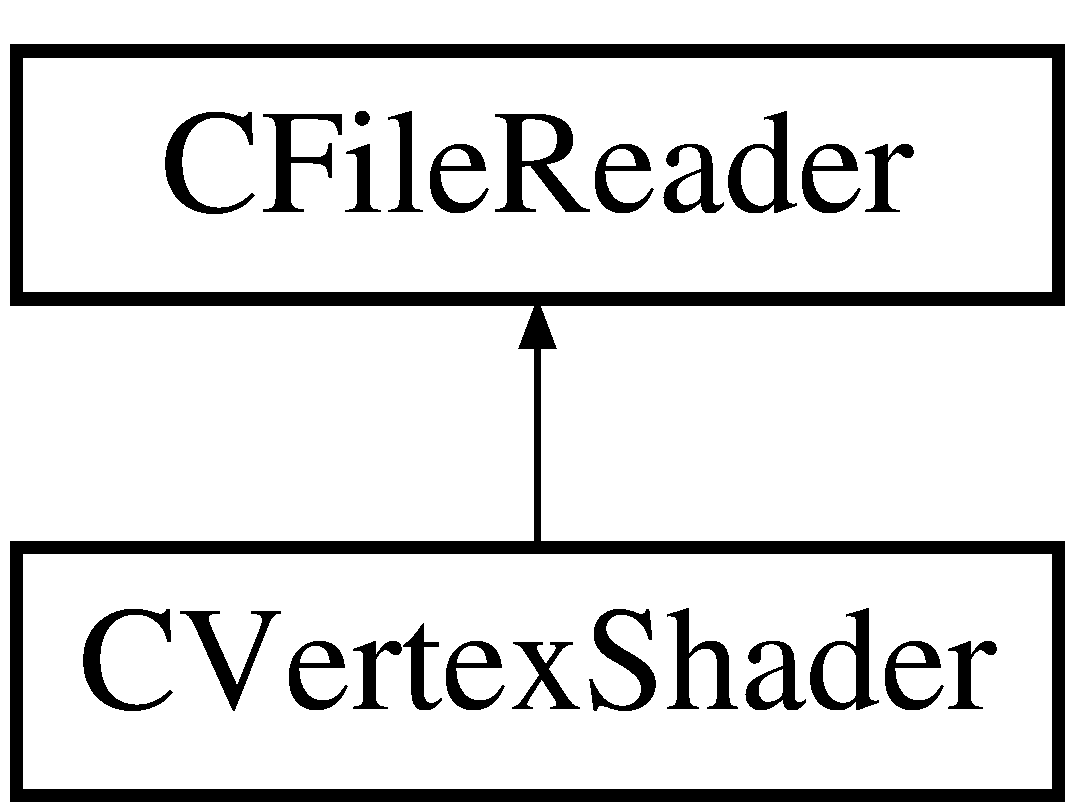
\includegraphics[height=2.000000cm]{class_c_vertex_shader}
\end{center}
\end{figure}
\subsection*{クラス}
\begin{DoxyCompactItemize}
\item 
struct \hyperlink{struct_c_vertex_shader_1_1_st_init_param}{St\+Init\+Param}
\begin{DoxyCompactList}\small\item\em 初期化用パラメータ。 \end{DoxyCompactList}\end{DoxyCompactItemize}
\subsection*{公開メンバ関数}
\begin{DoxyCompactItemize}
\item 
\hyperlink{class_c_vertex_shader_abe43f0c4eb007a656660fe85c6c7d759}{C\+Vertex\+Shader} (const \hyperlink{struct_c_vertex_shader_1_1_st_init_param}{St\+Init\+Param} \&\+\_\+rst\+Init\+Param)
\begin{DoxyCompactList}\small\item\em コンストラクタ。 \end{DoxyCompactList}\item 
virtual \hyperlink{class_c_vertex_shader_aecd16374bc117e251052ee75c67417c8}{$\sim$\+C\+Vertex\+Shader} ()
\begin{DoxyCompactList}\small\item\em デストラクタ。 \end{DoxyCompactList}\item 
virtual void \hyperlink{class_c_vertex_shader_a6e640bce4b58ca267c39b9287a973c3b}{Read\+End\+Process} (const void $\ast$\+\_\+p\+Data, U\+Size \+\_\+u\+Size) override
\begin{DoxyCompactList}\small\item\em 読み込み完了時の処理。 \end{DoxyCompactList}\item 
I\+D3\+D\+Vertex\+Shader $\ast$ \hyperlink{class_c_vertex_shader_a955aa28538cac1841a22245f088c604a}{Get\+Shader} () const 
\begin{DoxyCompactList}\small\item\em シェーダーを取得。 \end{DoxyCompactList}\item 
I\+D3\+D\+Input\+Layout $\ast$ \hyperlink{class_c_vertex_shader_a5b387308b2743e82c735507690c96307}{Get\+Input\+Layout} () const 
\begin{DoxyCompactList}\small\item\em 入力レイアウトを取得。 \end{DoxyCompactList}\end{DoxyCompactItemize}
\subsection*{非公開メンバ関数}
\begin{DoxyCompactItemize}
\item 
D\+X\+G\+I\+\_\+\+F\+O\+R\+M\+A\+T \hyperlink{class_c_vertex_shader_a5edf12786a3cde69a7ec082433a46562}{Get\+Dxgi\+Format} (D3\+D\+\_\+\+R\+E\+G\+I\+S\+T\+E\+R\+\_\+\+C\+O\+M\+P\+O\+N\+E\+N\+T\+\_\+\+T\+Y\+P\+E \+\_\+u\+Type, U32 \+\_\+u\+Mask)
\begin{DoxyCompactList}\small\item\em D\+X\+G\+Iフォーマットを取得。 \end{DoxyCompactList}\end{DoxyCompactItemize}
\subsection*{非公開変数類}
\begin{DoxyCompactItemize}
\item 
I\+D3\+D\+Vertex\+Shader $\ast$ \hyperlink{class_c_vertex_shader_af03968e57fbcebe385d94681b746c41c}{m\+\_\+pc\+Vertex\+Shader}
\item 
I\+D3\+D\+Input\+Layout $\ast$ \hyperlink{class_c_vertex_shader_a9194362254f16f3e89b0b0042c705a26}{m\+\_\+pc\+Input\+Layout}
\end{DoxyCompactItemize}


\subsection{構築子と解体子}
\hypertarget{class_c_vertex_shader_abe43f0c4eb007a656660fe85c6c7d759}{}\index{C\+Vertex\+Shader@{C\+Vertex\+Shader}!C\+Vertex\+Shader@{C\+Vertex\+Shader}}
\index{C\+Vertex\+Shader@{C\+Vertex\+Shader}!C\+Vertex\+Shader@{C\+Vertex\+Shader}}
\subsubsection[{C\+Vertex\+Shader(const St\+Init\+Param \&\+\_\+rst\+Init\+Param)}]{\setlength{\rightskip}{0pt plus 5cm}C\+Vertex\+Shader\+::\+C\+Vertex\+Shader (
\begin{DoxyParamCaption}
\item[{const {\bf St\+Init\+Param} \&}]{\+\_\+rst\+Init\+Param}
\end{DoxyParamCaption}
)}\label{class_c_vertex_shader_abe43f0c4eb007a656660fe85c6c7d759}


コンストラクタ。 


\begin{DoxyParams}[1]{引数}
\mbox{\tt in}  & {\em \+\_\+rst\+Init\+Param} & \+: 初期化用パラメータ。 \\
\hline
\end{DoxyParams}
\hypertarget{class_c_vertex_shader_aecd16374bc117e251052ee75c67417c8}{}\index{C\+Vertex\+Shader@{C\+Vertex\+Shader}!````~C\+Vertex\+Shader@{$\sim$\+C\+Vertex\+Shader}}
\index{````~C\+Vertex\+Shader@{$\sim$\+C\+Vertex\+Shader}!C\+Vertex\+Shader@{C\+Vertex\+Shader}}
\subsubsection[{$\sim$\+C\+Vertex\+Shader()}]{\setlength{\rightskip}{0pt plus 5cm}C\+Vertex\+Shader\+::$\sim$\+C\+Vertex\+Shader (
\begin{DoxyParamCaption}
{}
\end{DoxyParamCaption}
)\hspace{0.3cm}{\ttfamily [virtual]}}\label{class_c_vertex_shader_aecd16374bc117e251052ee75c67417c8}


デストラクタ。 



\subsection{関数詳解}
\hypertarget{class_c_vertex_shader_a5edf12786a3cde69a7ec082433a46562}{}\index{C\+Vertex\+Shader@{C\+Vertex\+Shader}!Get\+Dxgi\+Format@{Get\+Dxgi\+Format}}
\index{Get\+Dxgi\+Format@{Get\+Dxgi\+Format}!C\+Vertex\+Shader@{C\+Vertex\+Shader}}
\subsubsection[{Get\+Dxgi\+Format(\+D3\+D\+\_\+\+R\+E\+G\+I\+S\+T\+E\+R\+\_\+\+C\+O\+M\+P\+O\+N\+E\+N\+T\+\_\+\+T\+Y\+P\+E \+\_\+u\+Type, U32 \+\_\+u\+Mask)}]{\setlength{\rightskip}{0pt plus 5cm}D\+X\+G\+I\+\_\+\+F\+O\+R\+M\+A\+T C\+Vertex\+Shader\+::\+Get\+Dxgi\+Format (
\begin{DoxyParamCaption}
\item[{D3\+D\+\_\+\+R\+E\+G\+I\+S\+T\+E\+R\+\_\+\+C\+O\+M\+P\+O\+N\+E\+N\+T\+\_\+\+T\+Y\+P\+E}]{\+\_\+u\+Type, }
\item[{U32}]{\+\_\+u\+Mask}
\end{DoxyParamCaption}
)\hspace{0.3cm}{\ttfamily [private]}}\label{class_c_vertex_shader_a5edf12786a3cde69a7ec082433a46562}


D\+X\+G\+Iフォーマットを取得。 

D\+X\+G\+Iフォーマットの取得。


\begin{DoxyParams}[1]{引数}
\mbox{\tt in}  & {\em \+\_\+u\+Type} & \+: フォーマットタイプ。 \\
\hline
\mbox{\tt in}  & {\em \+\_\+u\+Mask} & \+: マスク(xyzwを使用しているか。) \\
\hline
\end{DoxyParams}
\begin{DoxyNote}{覚え書き}
floatにしか対応していません。他の型を使用する場合は処理を追加する必要があります。 
\end{DoxyNote}
\hypertarget{class_c_vertex_shader_a5b387308b2743e82c735507690c96307}{}\index{C\+Vertex\+Shader@{C\+Vertex\+Shader}!Get\+Input\+Layout@{Get\+Input\+Layout}}
\index{Get\+Input\+Layout@{Get\+Input\+Layout}!C\+Vertex\+Shader@{C\+Vertex\+Shader}}
\subsubsection[{Get\+Input\+Layout() const }]{\setlength{\rightskip}{0pt plus 5cm}I\+D3\+D\+Input\+Layout$\ast$ C\+Vertex\+Shader\+::\+Get\+Input\+Layout (
\begin{DoxyParamCaption}
{}
\end{DoxyParamCaption}
) const\hspace{0.3cm}{\ttfamily [inline]}}\label{class_c_vertex_shader_a5b387308b2743e82c735507690c96307}


入力レイアウトを取得。 

\hypertarget{class_c_vertex_shader_a955aa28538cac1841a22245f088c604a}{}\index{C\+Vertex\+Shader@{C\+Vertex\+Shader}!Get\+Shader@{Get\+Shader}}
\index{Get\+Shader@{Get\+Shader}!C\+Vertex\+Shader@{C\+Vertex\+Shader}}
\subsubsection[{Get\+Shader() const }]{\setlength{\rightskip}{0pt plus 5cm}I\+D3\+D\+Vertex\+Shader$\ast$ C\+Vertex\+Shader\+::\+Get\+Shader (
\begin{DoxyParamCaption}
{}
\end{DoxyParamCaption}
) const\hspace{0.3cm}{\ttfamily [inline]}}\label{class_c_vertex_shader_a955aa28538cac1841a22245f088c604a}


シェーダーを取得。 

\hypertarget{class_c_vertex_shader_a6e640bce4b58ca267c39b9287a973c3b}{}\index{C\+Vertex\+Shader@{C\+Vertex\+Shader}!Read\+End\+Process@{Read\+End\+Process}}
\index{Read\+End\+Process@{Read\+End\+Process}!C\+Vertex\+Shader@{C\+Vertex\+Shader}}
\subsubsection[{Read\+End\+Process(const void $\ast$\+\_\+p\+Data, U\+Size \+\_\+u\+Size) override}]{\setlength{\rightskip}{0pt plus 5cm}void C\+Vertex\+Shader\+::\+Read\+End\+Process (
\begin{DoxyParamCaption}
\item[{const void $\ast$}]{\+\_\+p\+Data, }
\item[{U\+Size}]{\+\_\+u\+Size}
\end{DoxyParamCaption}
)\hspace{0.3cm}{\ttfamily [override]}, {\ttfamily [virtual]}}\label{class_c_vertex_shader_a6e640bce4b58ca267c39b9287a973c3b}


読み込み完了時の処理。 


\begin{DoxyParams}[1]{引数}
\mbox{\tt in}  & {\em \+\_\+p\+Data} & \+: 読み込んだデータ。 \\
\hline
\mbox{\tt in}  & {\em \+\_\+u\+Size} & \+: 読み込んだデータサイズ。 \\
\hline
\end{DoxyParams}


\hyperlink{class_c_file_reader_a5a18550133826ac43096629f6eaa8c42}{C\+File\+Reader}を再実装しています。



\subsection{メンバ詳解}
\hypertarget{class_c_vertex_shader_a9194362254f16f3e89b0b0042c705a26}{}\index{C\+Vertex\+Shader@{C\+Vertex\+Shader}!m\+\_\+pc\+Input\+Layout@{m\+\_\+pc\+Input\+Layout}}
\index{m\+\_\+pc\+Input\+Layout@{m\+\_\+pc\+Input\+Layout}!C\+Vertex\+Shader@{C\+Vertex\+Shader}}
\subsubsection[{m\+\_\+pc\+Input\+Layout}]{\setlength{\rightskip}{0pt plus 5cm}I\+D3\+D\+Input\+Layout$\ast$ C\+Vertex\+Shader\+::m\+\_\+pc\+Input\+Layout\hspace{0.3cm}{\ttfamily [private]}}\label{class_c_vertex_shader_a9194362254f16f3e89b0b0042c705a26}
\hypertarget{class_c_vertex_shader_af03968e57fbcebe385d94681b746c41c}{}\index{C\+Vertex\+Shader@{C\+Vertex\+Shader}!m\+\_\+pc\+Vertex\+Shader@{m\+\_\+pc\+Vertex\+Shader}}
\index{m\+\_\+pc\+Vertex\+Shader@{m\+\_\+pc\+Vertex\+Shader}!C\+Vertex\+Shader@{C\+Vertex\+Shader}}
\subsubsection[{m\+\_\+pc\+Vertex\+Shader}]{\setlength{\rightskip}{0pt plus 5cm}I\+D3\+D\+Vertex\+Shader$\ast$ C\+Vertex\+Shader\+::m\+\_\+pc\+Vertex\+Shader\hspace{0.3cm}{\ttfamily [private]}}\label{class_c_vertex_shader_af03968e57fbcebe385d94681b746c41c}


このクラス詳解は次のファイルから抽出されました\+:\begin{DoxyCompactItemize}
\item 
D\+:/\+Project/\+Game/\+Lib/\+Direct\+X/\hyperlink{_vertex_shader_8h}{Vertex\+Shader.\+h}\item 
D\+:/\+Project/\+Game/\+Lib/\+Direct\+X/\hyperlink{_vertex_shader_8cpp}{Vertex\+Shader.\+cpp}\end{DoxyCompactItemize}

\hypertarget{class_c_win_base}{}\section{C\+Win\+Base クラス}
\label{class_c_win_base}\index{C\+Win\+Base@{C\+Win\+Base}}


{\ttfamily \#include $<$Win\+Base.\+h$>$}

C\+Win\+Base の継承関係図\begin{figure}[H]
\begin{center}
\leavevmode
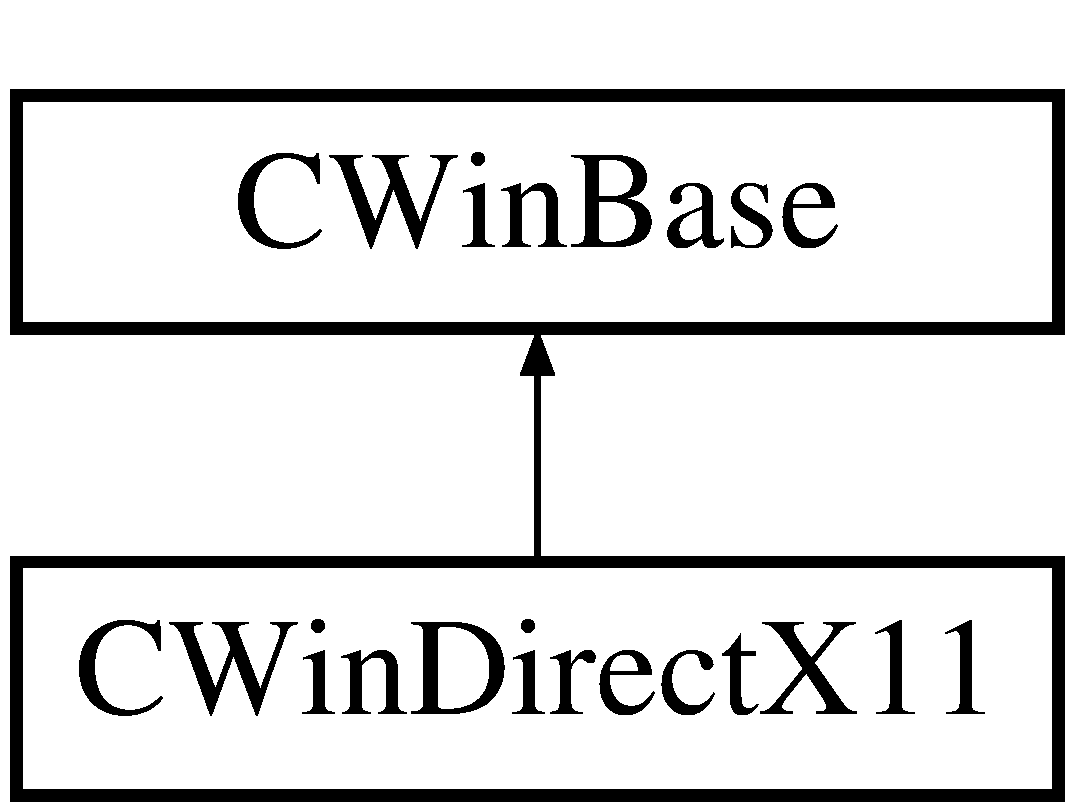
\includegraphics[height=2.000000cm]{class_c_win_base}
\end{center}
\end{figure}
\subsection*{クラス}
\begin{DoxyCompactItemize}
\item 
struct \hyperlink{struct_c_win_base_1_1_st_init_param}{St\+Init\+Param}
\begin{DoxyCompactList}\small\item\em 初期化用パラメータ。 \end{DoxyCompactList}\end{DoxyCompactItemize}
\subsection*{公開メンバ関数}
\begin{DoxyCompactItemize}
\item 
\hyperlink{class_c_win_base_a61c9bced0a9d9cdcbbed44ad5d555a68}{C\+Win\+Base} (const \hyperlink{struct_c_win_base_1_1_st_init_param}{St\+Init\+Param} \&\+\_\+rst\+Init\+Param)
\begin{DoxyCompactList}\small\item\em コンストラクタ。 \end{DoxyCompactList}\item 
virtual \hyperlink{class_c_win_base_a7d8eda9e0a576178dc7c86967b6e9626}{$\sim$\+C\+Win\+Base} ()
\begin{DoxyCompactList}\small\item\em デストラクタ。 \end{DoxyCompactList}\item 
bool \hyperlink{class_c_win_base_ac9d42b98ac82db19bd562615fa9decd7}{Init\+Window} ()
\begin{DoxyCompactList}\small\item\em ウィンドウの初期化。 \end{DoxyCompactList}\item 
virtual L\+R\+E\+S\+U\+L\+T \hyperlink{class_c_win_base_a3c4c86f97de4eddaa300a73c952c84b2}{Wnd\+Proc} (H\+W\+N\+D \+\_\+h\+Wnd, U\+I\+N\+T \+\_\+u\+Msg, W\+P\+A\+R\+A\+M \+\_\+u\+W\+Param, L\+P\+A\+R\+A\+M \+\_\+u\+L\+Param)
\item 
S32 \hyperlink{class_c_win_base_a9f6a1a2c0b539863b6ad0fab052196dd}{Get\+Width} () const 
\begin{DoxyCompactList}\small\item\em ウィンドウの幅を取得。 \end{DoxyCompactList}\item 
S32 \hyperlink{class_c_win_base_ab283c793e272287f91e58e8ac9f31c63}{Get\+Height} () const 
\begin{DoxyCompactList}\small\item\em ウィンドウの高さを取得。 \end{DoxyCompactList}\item 
H\+W\+N\+D \hyperlink{class_c_win_base_afc7879c3e92a6a9a912191a0c318f25c}{Get\+Window\+Handle} () const 
\begin{DoxyCompactList}\small\item\em ウィンドウハンドルを取得。 \end{DoxyCompactList}\end{DoxyCompactItemize}
\subsection*{静的公開メンバ関数}
\begin{DoxyCompactItemize}
\item 
static L\+R\+E\+S\+U\+L\+T C\+A\+L\+L\+B\+A\+C\+K \hyperlink{class_c_win_base_a6aeddce777aab9aa11122ad0a4c87287}{Wnd\+Proc\+Wrapper} (H\+W\+N\+D \+\_\+h\+Wnd, U\+I\+N\+T \+\_\+u\+Msg, W\+P\+A\+R\+A\+M \+\_\+u\+W\+Param, L\+P\+A\+R\+A\+M \+\_\+u\+L\+Param)
\begin{DoxyCompactList}\small\item\em ウィンドウプロシージャ。 \end{DoxyCompactList}\end{DoxyCompactItemize}
\subsection*{限定公開変数類}
\begin{DoxyCompactItemize}
\item 
\hyperlink{struct_c_win_base_1_1_st_init_param}{St\+Init\+Param} \hyperlink{class_c_win_base_abffc43f13e4878d093ffb0014cdad8a4}{m\+\_\+st\+Init\+Param}
\begin{DoxyCompactList}\small\item\em 初期化用パラメータ。 \end{DoxyCompactList}\item 
\hyperlink{_string_8h_a65b002fe7fe31f6e84dbb7e46907e031}{C\+T\+String} \hyperlink{class_c_win_base_a51dd5d7b97d383a2262d398926afd69f}{m\+\_\+c\+Class\+Name}
\begin{DoxyCompactList}\small\item\em クラス名。 \end{DoxyCompactList}\item 
\hyperlink{_string_8h_a65b002fe7fe31f6e84dbb7e46907e031}{C\+T\+String} \hyperlink{class_c_win_base_a167e6b8f4adb4f249e45147a84c47c9e}{m\+\_\+c\+Window\+Name}
\begin{DoxyCompactList}\small\item\em ウィンドウ名。 \end{DoxyCompactList}\item 
H\+W\+N\+D \hyperlink{class_c_win_base_acbf763d98e40063d0676af4279a619a3}{m\+\_\+h\+Wnd}
\end{DoxyCompactItemize}


\subsection{構築子と解体子}
\hypertarget{class_c_win_base_a61c9bced0a9d9cdcbbed44ad5d555a68}{}\index{C\+Win\+Base@{C\+Win\+Base}!C\+Win\+Base@{C\+Win\+Base}}
\index{C\+Win\+Base@{C\+Win\+Base}!C\+Win\+Base@{C\+Win\+Base}}
\subsubsection[{C\+Win\+Base(const St\+Init\+Param \&\+\_\+rst\+Init\+Param)}]{\setlength{\rightskip}{0pt plus 5cm}C\+Win\+Base\+::\+C\+Win\+Base (
\begin{DoxyParamCaption}
\item[{const {\bf St\+Init\+Param} \&}]{\+\_\+rst\+Init\+Param}
\end{DoxyParamCaption}
)}\label{class_c_win_base_a61c9bced0a9d9cdcbbed44ad5d555a68}


コンストラクタ。 


\begin{DoxyParams}[1]{引数}
\mbox{\tt in}  & {\em \+\_\+rst\+Init\+Param} & \+: 初期化用パラメータ。 \\
\hline
\end{DoxyParams}
\hypertarget{class_c_win_base_a7d8eda9e0a576178dc7c86967b6e9626}{}\index{C\+Win\+Base@{C\+Win\+Base}!````~C\+Win\+Base@{$\sim$\+C\+Win\+Base}}
\index{````~C\+Win\+Base@{$\sim$\+C\+Win\+Base}!C\+Win\+Base@{C\+Win\+Base}}
\subsubsection[{$\sim$\+C\+Win\+Base()}]{\setlength{\rightskip}{0pt plus 5cm}virtual C\+Win\+Base\+::$\sim$\+C\+Win\+Base (
\begin{DoxyParamCaption}
{}
\end{DoxyParamCaption}
)\hspace{0.3cm}{\ttfamily [inline]}, {\ttfamily [virtual]}}\label{class_c_win_base_a7d8eda9e0a576178dc7c86967b6e9626}


デストラクタ。 



\subsection{関数詳解}
\hypertarget{class_c_win_base_ab283c793e272287f91e58e8ac9f31c63}{}\index{C\+Win\+Base@{C\+Win\+Base}!Get\+Height@{Get\+Height}}
\index{Get\+Height@{Get\+Height}!C\+Win\+Base@{C\+Win\+Base}}
\subsubsection[{Get\+Height() const }]{\setlength{\rightskip}{0pt plus 5cm}S32 C\+Win\+Base\+::\+Get\+Height (
\begin{DoxyParamCaption}
{}
\end{DoxyParamCaption}
) const\hspace{0.3cm}{\ttfamily [inline]}}\label{class_c_win_base_ab283c793e272287f91e58e8ac9f31c63}


ウィンドウの高さを取得。 

\hypertarget{class_c_win_base_a9f6a1a2c0b539863b6ad0fab052196dd}{}\index{C\+Win\+Base@{C\+Win\+Base}!Get\+Width@{Get\+Width}}
\index{Get\+Width@{Get\+Width}!C\+Win\+Base@{C\+Win\+Base}}
\subsubsection[{Get\+Width() const }]{\setlength{\rightskip}{0pt plus 5cm}S32 C\+Win\+Base\+::\+Get\+Width (
\begin{DoxyParamCaption}
{}
\end{DoxyParamCaption}
) const\hspace{0.3cm}{\ttfamily [inline]}}\label{class_c_win_base_a9f6a1a2c0b539863b6ad0fab052196dd}


ウィンドウの幅を取得。 

\hypertarget{class_c_win_base_afc7879c3e92a6a9a912191a0c318f25c}{}\index{C\+Win\+Base@{C\+Win\+Base}!Get\+Window\+Handle@{Get\+Window\+Handle}}
\index{Get\+Window\+Handle@{Get\+Window\+Handle}!C\+Win\+Base@{C\+Win\+Base}}
\subsubsection[{Get\+Window\+Handle() const }]{\setlength{\rightskip}{0pt plus 5cm}H\+W\+N\+D C\+Win\+Base\+::\+Get\+Window\+Handle (
\begin{DoxyParamCaption}
{}
\end{DoxyParamCaption}
) const\hspace{0.3cm}{\ttfamily [inline]}}\label{class_c_win_base_afc7879c3e92a6a9a912191a0c318f25c}


ウィンドウハンドルを取得。 

\hypertarget{class_c_win_base_ac9d42b98ac82db19bd562615fa9decd7}{}\index{C\+Win\+Base@{C\+Win\+Base}!Init\+Window@{Init\+Window}}
\index{Init\+Window@{Init\+Window}!C\+Win\+Base@{C\+Win\+Base}}
\subsubsection[{Init\+Window()}]{\setlength{\rightskip}{0pt plus 5cm}bool C\+Win\+Base\+::\+Init\+Window (
\begin{DoxyParamCaption}
{}
\end{DoxyParamCaption}
)}\label{class_c_win_base_ac9d42b98ac82db19bd562615fa9decd7}


ウィンドウの初期化。 

ウィンドウの作成。 \hypertarget{class_c_win_base_a3c4c86f97de4eddaa300a73c952c84b2}{}\index{C\+Win\+Base@{C\+Win\+Base}!Wnd\+Proc@{Wnd\+Proc}}
\index{Wnd\+Proc@{Wnd\+Proc}!C\+Win\+Base@{C\+Win\+Base}}
\subsubsection[{Wnd\+Proc(\+H\+W\+N\+D \+\_\+h\+Wnd, U\+I\+N\+T \+\_\+u\+Msg, W\+P\+A\+R\+A\+M \+\_\+u\+W\+Param, L\+P\+A\+R\+A\+M \+\_\+u\+L\+Param)}]{\setlength{\rightskip}{0pt plus 5cm}L\+R\+E\+S\+U\+L\+T C\+Win\+Base\+::\+Wnd\+Proc (
\begin{DoxyParamCaption}
\item[{H\+W\+N\+D}]{\+\_\+h\+Wnd, }
\item[{U\+I\+N\+T}]{\+\_\+u\+Msg, }
\item[{W\+P\+A\+R\+A\+M}]{\+\_\+u\+W\+Param, }
\item[{L\+P\+A\+R\+A\+M}]{\+\_\+u\+L\+Param}
\end{DoxyParamCaption}
)\hspace{0.3cm}{\ttfamily [virtual]}}\label{class_c_win_base_a3c4c86f97de4eddaa300a73c952c84b2}


\hyperlink{class_c_win_direct_x11_aac1053a3e7bba9cd66e60e45f754a06e}{C\+Win\+Direct\+X11}で再実装されています。

\hypertarget{class_c_win_base_a6aeddce777aab9aa11122ad0a4c87287}{}\index{C\+Win\+Base@{C\+Win\+Base}!Wnd\+Proc\+Wrapper@{Wnd\+Proc\+Wrapper}}
\index{Wnd\+Proc\+Wrapper@{Wnd\+Proc\+Wrapper}!C\+Win\+Base@{C\+Win\+Base}}
\subsubsection[{Wnd\+Proc\+Wrapper(\+H\+W\+N\+D \+\_\+h\+Wnd, U\+I\+N\+T \+\_\+u\+Msg, W\+P\+A\+R\+A\+M \+\_\+u\+W\+Param, L\+P\+A\+R\+A\+M \+\_\+u\+L\+Param)}]{\setlength{\rightskip}{0pt plus 5cm}L\+R\+E\+S\+U\+L\+T C\+A\+L\+L\+B\+A\+C\+K C\+Win\+Base\+::\+Wnd\+Proc\+Wrapper (
\begin{DoxyParamCaption}
\item[{H\+W\+N\+D}]{\+\_\+h\+Wnd, }
\item[{U\+I\+N\+T}]{\+\_\+u\+Msg, }
\item[{W\+P\+A\+R\+A\+M}]{\+\_\+u\+W\+Param, }
\item[{L\+P\+A\+R\+A\+M}]{\+\_\+u\+L\+Param}
\end{DoxyParamCaption}
)\hspace{0.3cm}{\ttfamily [static]}}\label{class_c_win_base_a6aeddce777aab9aa11122ad0a4c87287}


ウィンドウプロシージャ。 


\begin{DoxyParams}[1]{引数}
\mbox{\tt in}  & {\em \+\_\+h\+Wnd} & \+: ウィンドウハンドル。 \\
\hline
\mbox{\tt in}  & {\em \+\_\+u\+Msg} & \+: メッセージ。 \\
\hline
\mbox{\tt in}  & {\em \+\_\+u\+W\+Param} & \+: パラメータ。 \\
\hline
\mbox{\tt in}  & {\em \+\_\+u\+L\+Param} & \+: パラメータ。 \\
\hline
\end{DoxyParams}

\begin{DoxyRetVals}{戻り値}
{\em L\+R\+E\+S\+U\+L\+T} & \+: 処理結果。 \\
\hline
\end{DoxyRetVals}


\subsection{メンバ詳解}
\hypertarget{class_c_win_base_a51dd5d7b97d383a2262d398926afd69f}{}\index{C\+Win\+Base@{C\+Win\+Base}!m\+\_\+c\+Class\+Name@{m\+\_\+c\+Class\+Name}}
\index{m\+\_\+c\+Class\+Name@{m\+\_\+c\+Class\+Name}!C\+Win\+Base@{C\+Win\+Base}}
\subsubsection[{m\+\_\+c\+Class\+Name}]{\setlength{\rightskip}{0pt plus 5cm}{\bf C\+T\+String} C\+Win\+Base\+::m\+\_\+c\+Class\+Name\hspace{0.3cm}{\ttfamily [protected]}}\label{class_c_win_base_a51dd5d7b97d383a2262d398926afd69f}


クラス名。 

\hypertarget{class_c_win_base_a167e6b8f4adb4f249e45147a84c47c9e}{}\index{C\+Win\+Base@{C\+Win\+Base}!m\+\_\+c\+Window\+Name@{m\+\_\+c\+Window\+Name}}
\index{m\+\_\+c\+Window\+Name@{m\+\_\+c\+Window\+Name}!C\+Win\+Base@{C\+Win\+Base}}
\subsubsection[{m\+\_\+c\+Window\+Name}]{\setlength{\rightskip}{0pt plus 5cm}{\bf C\+T\+String} C\+Win\+Base\+::m\+\_\+c\+Window\+Name\hspace{0.3cm}{\ttfamily [protected]}}\label{class_c_win_base_a167e6b8f4adb4f249e45147a84c47c9e}


ウィンドウ名。 

\hypertarget{class_c_win_base_acbf763d98e40063d0676af4279a619a3}{}\index{C\+Win\+Base@{C\+Win\+Base}!m\+\_\+h\+Wnd@{m\+\_\+h\+Wnd}}
\index{m\+\_\+h\+Wnd@{m\+\_\+h\+Wnd}!C\+Win\+Base@{C\+Win\+Base}}
\subsubsection[{m\+\_\+h\+Wnd}]{\setlength{\rightskip}{0pt plus 5cm}H\+W\+N\+D C\+Win\+Base\+::m\+\_\+h\+Wnd\hspace{0.3cm}{\ttfamily [protected]}}\label{class_c_win_base_acbf763d98e40063d0676af4279a619a3}
\hypertarget{class_c_win_base_abffc43f13e4878d093ffb0014cdad8a4}{}\index{C\+Win\+Base@{C\+Win\+Base}!m\+\_\+st\+Init\+Param@{m\+\_\+st\+Init\+Param}}
\index{m\+\_\+st\+Init\+Param@{m\+\_\+st\+Init\+Param}!C\+Win\+Base@{C\+Win\+Base}}
\subsubsection[{m\+\_\+st\+Init\+Param}]{\setlength{\rightskip}{0pt plus 5cm}{\bf St\+Init\+Param} C\+Win\+Base\+::m\+\_\+st\+Init\+Param\hspace{0.3cm}{\ttfamily [protected]}}\label{class_c_win_base_abffc43f13e4878d093ffb0014cdad8a4}


初期化用パラメータ。 



このクラス詳解は次のファイルから抽出されました\+:\begin{DoxyCompactItemize}
\item 
D\+:/\+Project/\+Game/\+Windows/\hyperlink{_win_base_8h}{Win\+Base.\+h}\item 
D\+:/\+Project/\+Game/\+Windows/\hyperlink{_win_base_8cpp}{Win\+Base.\+cpp}\end{DoxyCompactItemize}

\hypertarget{class_c_win_direct_x11}{}\section{C\+Win\+Direct\+X11 クラス}
\label{class_c_win_direct_x11}\index{C\+Win\+Direct\+X11@{C\+Win\+Direct\+X11}}


{\ttfamily \#include $<$Win\+Direct\+X11.\+h$>$}

C\+Win\+Direct\+X11 の継承関係図\begin{figure}[H]
\begin{center}
\leavevmode
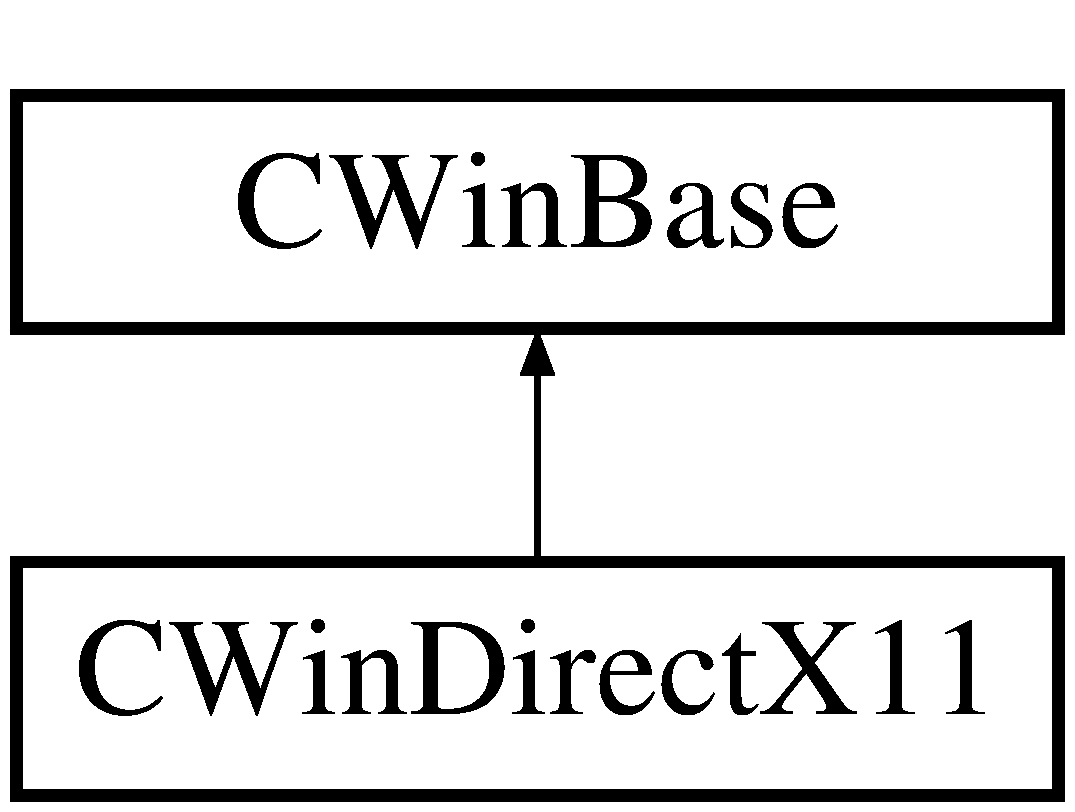
\includegraphics[height=2.000000cm]{class_c_win_direct_x11}
\end{center}
\end{figure}
\subsection*{公開メンバ関数}
\begin{DoxyCompactItemize}
\item 
\hyperlink{class_c_win_direct_x11_a3fa4a47732c85ab2c0646afe56be4617}{C\+Win\+Direct\+X11} (const \hyperlink{struct_c_win_base_1_1_st_init_param}{St\+Init\+Param} \&\+\_\+rst\+Init\+Param)
\begin{DoxyCompactList}\small\item\em コンストラクタ。 \end{DoxyCompactList}\item 
virtual \hyperlink{class_c_win_direct_x11_ad26e687caf4b1cb793466119e657b150}{$\sim$\+C\+Win\+Direct\+X11} ()
\begin{DoxyCompactList}\small\item\em デストラクタ。 \end{DoxyCompactList}\item 
virtual L\+R\+E\+S\+U\+L\+T \hyperlink{class_c_win_direct_x11_aac1053a3e7bba9cd66e60e45f754a06e}{Wnd\+Proc} (H\+W\+N\+D \+\_\+h\+Wnd, U\+I\+N\+T \+\_\+u\+Msg, W\+P\+A\+R\+A\+M \+\_\+u\+W\+Param, L\+P\+A\+R\+A\+M \+\_\+u\+L\+Param) final
\begin{DoxyCompactList}\small\item\em ウィンドウプロシージャ。 \end{DoxyCompactList}\end{DoxyCompactItemize}
\subsection*{その他の継承メンバ}


\subsection{構築子と解体子}
\hypertarget{class_c_win_direct_x11_a3fa4a47732c85ab2c0646afe56be4617}{}\index{C\+Win\+Direct\+X11@{C\+Win\+Direct\+X11}!C\+Win\+Direct\+X11@{C\+Win\+Direct\+X11}}
\index{C\+Win\+Direct\+X11@{C\+Win\+Direct\+X11}!C\+Win\+Direct\+X11@{C\+Win\+Direct\+X11}}
\subsubsection[{C\+Win\+Direct\+X11(const St\+Init\+Param \&\+\_\+rst\+Init\+Param)}]{\setlength{\rightskip}{0pt plus 5cm}C\+Win\+Direct\+X11\+::\+C\+Win\+Direct\+X11 (
\begin{DoxyParamCaption}
\item[{const {\bf St\+Init\+Param} \&}]{\+\_\+rst\+Init\+Param}
\end{DoxyParamCaption}
)}\label{class_c_win_direct_x11_a3fa4a47732c85ab2c0646afe56be4617}


コンストラクタ。 


\begin{DoxyParams}[1]{引数}
\mbox{\tt in}  & {\em \+\_\+rst\+Init\+Param} & \+: 初期化用パラメータ。 \\
\hline
\end{DoxyParams}
\hypertarget{class_c_win_direct_x11_ad26e687caf4b1cb793466119e657b150}{}\index{C\+Win\+Direct\+X11@{C\+Win\+Direct\+X11}!````~C\+Win\+Direct\+X11@{$\sim$\+C\+Win\+Direct\+X11}}
\index{````~C\+Win\+Direct\+X11@{$\sim$\+C\+Win\+Direct\+X11}!C\+Win\+Direct\+X11@{C\+Win\+Direct\+X11}}
\subsubsection[{$\sim$\+C\+Win\+Direct\+X11()}]{\setlength{\rightskip}{0pt plus 5cm}C\+Win\+Direct\+X11\+::$\sim$\+C\+Win\+Direct\+X11 (
\begin{DoxyParamCaption}
{}
\end{DoxyParamCaption}
)\hspace{0.3cm}{\ttfamily [virtual]}}\label{class_c_win_direct_x11_ad26e687caf4b1cb793466119e657b150}


デストラクタ。 



\subsection{関数詳解}
\hypertarget{class_c_win_direct_x11_aac1053a3e7bba9cd66e60e45f754a06e}{}\index{C\+Win\+Direct\+X11@{C\+Win\+Direct\+X11}!Wnd\+Proc@{Wnd\+Proc}}
\index{Wnd\+Proc@{Wnd\+Proc}!C\+Win\+Direct\+X11@{C\+Win\+Direct\+X11}}
\subsubsection[{Wnd\+Proc(\+H\+W\+N\+D \+\_\+h\+Wnd, U\+I\+N\+T \+\_\+u\+Msg, W\+P\+A\+R\+A\+M \+\_\+u\+W\+Param, L\+P\+A\+R\+A\+M \+\_\+u\+L\+Param) final}]{\setlength{\rightskip}{0pt plus 5cm}L\+R\+E\+S\+U\+L\+T C\+Win\+Direct\+X11\+::\+Wnd\+Proc (
\begin{DoxyParamCaption}
\item[{H\+W\+N\+D}]{\+\_\+h\+Wnd, }
\item[{U\+I\+N\+T}]{\+\_\+u\+Msg, }
\item[{W\+P\+A\+R\+A\+M}]{\+\_\+u\+W\+Param, }
\item[{L\+P\+A\+R\+A\+M}]{\+\_\+u\+L\+Param}
\end{DoxyParamCaption}
)\hspace{0.3cm}{\ttfamily [final]}, {\ttfamily [virtual]}}\label{class_c_win_direct_x11_aac1053a3e7bba9cd66e60e45f754a06e}


ウィンドウプロシージャ。 


\begin{DoxyParams}[1]{引数}
\mbox{\tt in}  & {\em \+\_\+h\+Wnd} & \+: ウィンドウハンドル。 \\
\hline
\mbox{\tt in}  & {\em \+\_\+u\+Msg} & \+: メッセージ。 \\
\hline
\mbox{\tt in}  & {\em \+\_\+u\+W\+Param} & \+: パラメータ。 \\
\hline
\mbox{\tt in}  & {\em \+\_\+u\+L\+Param} & \+: パラメータ。 \\
\hline
\end{DoxyParams}

\begin{DoxyRetVals}{戻り値}
{\em L\+R\+E\+S\+U\+L\+T} & \+: 処理結果。 \\
\hline
\end{DoxyRetVals}


\hyperlink{class_c_win_base_a3c4c86f97de4eddaa300a73c952c84b2}{C\+Win\+Base}を再実装しています。



このクラス詳解は次のファイルから抽出されました\+:\begin{DoxyCompactItemize}
\item 
D\+:/\+Project/\+Game/\+Windows/\hyperlink{_win_direct_x11_8h}{Win\+Direct\+X11.\+h}\item 
D\+:/\+Project/\+Game/\+Windows/\hyperlink{_win_direct_x11_8cpp}{Win\+Direct\+X11.\+cpp}\end{DoxyCompactItemize}

\hypertarget{class_c_worker}{}\section{C\+Worker クラス}
\label{class_c_worker}\index{C\+Worker@{C\+Worker}}


{\ttfamily \#include $<$Worker.\+h$>$}

C\+Worker の継承関係図\begin{figure}[H]
\begin{center}
\leavevmode
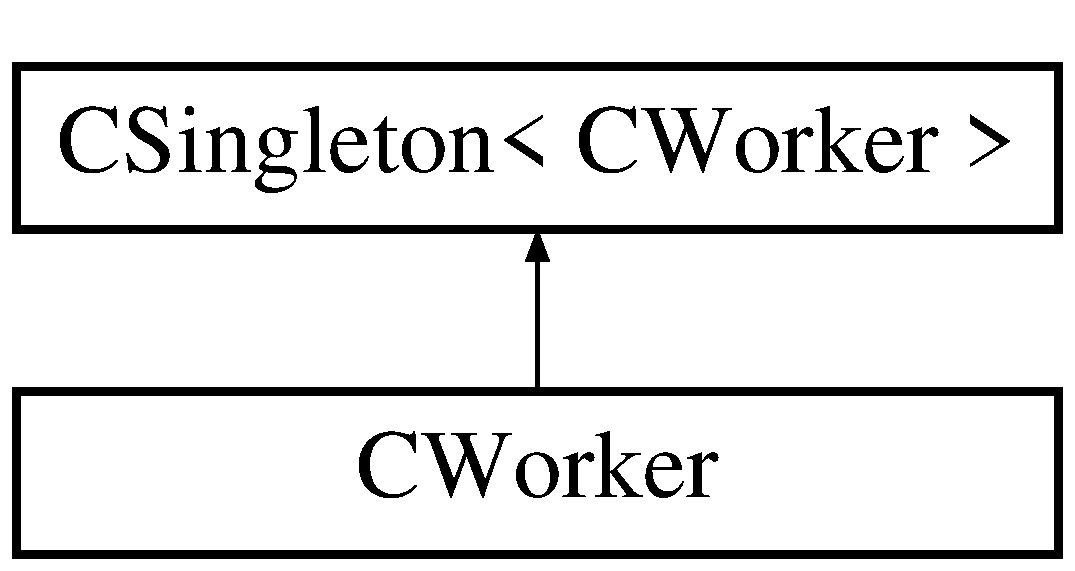
\includegraphics[height=2.000000cm]{class_c_worker}
\end{center}
\end{figure}
\subsection*{クラス}
\begin{DoxyCompactItemize}
\item 
struct \hyperlink{struct_c_worker_1_1_st_init_param}{St\+Init\+Param}
\begin{DoxyCompactList}\small\item\em 初期化用パラメータ。 \end{DoxyCompactList}\end{DoxyCompactItemize}
\subsection*{公開メンバ関数}
\begin{DoxyCompactItemize}
\item 
virtual \hyperlink{class_c_worker_ad7463ab6b440816bc9b8c1b2da167407}{$\sim$\+C\+Worker} ()
\begin{DoxyCompactList}\small\item\em デストラクタ。 \end{DoxyCompactList}\item 
void \hyperlink{class_c_worker_ad5d23dd82cbc33909e00146dfc5b039b}{Init} (const \hyperlink{struct_c_worker_1_1_st_init_param}{St\+Init\+Param} \&\+\_\+rst\+Init)
\begin{DoxyCompactList}\small\item\em 初期化。 \end{DoxyCompactList}\end{DoxyCompactItemize}
\subsection*{静的公開メンバ関数}
\begin{DoxyCompactItemize}
\item 
static void \hyperlink{class_c_worker_ad8d0e6b957ab9d84b6fe6290b564f23d}{Request\+Job} (\hyperlink{class_c_job}{C\+Job} $\ast$\+\_\+pc\+Job, bool \+\_\+b\+Sync)
\begin{DoxyCompactList}\small\item\em リクエスト。 \end{DoxyCompactList}\item 
static void \hyperlink{class_c_worker_a0cf70f37ffdadae5afb4606bd989ba6b}{Sync} ()
\begin{DoxyCompactList}\small\item\em 同期。 \end{DoxyCompactList}\end{DoxyCompactItemize}
\subsection*{非公開メンバ関数}
\begin{DoxyCompactItemize}
\item 
\hyperlink{class_c_worker_ab70f18344c40b5492db3836891d53990}{C\+Worker} ()
\begin{DoxyCompactList}\small\item\em コンストラクタ。 \end{DoxyCompactList}\end{DoxyCompactItemize}
\subsection*{非公開変数類}
\begin{DoxyCompactItemize}
\item 
friend \hyperlink{class_c_worker_aecbc638ed646f882a08fe4b6d6c4653c}{C\+Singleton$<$ C\+Worker $>$}
\item 
\hyperlink{class_c_worker_manager}{C\+Worker\+Manager} $\ast$ \hyperlink{class_c_worker_ae982e4473bdc5cee56f351c9888007f5}{m\+\_\+pc\+Worker\+Manager\+Sync}
\item 
\hyperlink{class_c_worker_manager}{C\+Worker\+Manager} $\ast$ \hyperlink{class_c_worker_ab96d974805f466c392897f55cd13e000}{m\+\_\+pc\+Worker\+Manager\+Un\+Sync}
\end{DoxyCompactItemize}
\subsection*{その他の継承メンバ}


\subsection{構築子と解体子}
\hypertarget{class_c_worker_ab70f18344c40b5492db3836891d53990}{}\index{C\+Worker@{C\+Worker}!C\+Worker@{C\+Worker}}
\index{C\+Worker@{C\+Worker}!C\+Worker@{C\+Worker}}
\subsubsection[{C\+Worker()}]{\setlength{\rightskip}{0pt plus 5cm}C\+Worker\+::\+C\+Worker (
\begin{DoxyParamCaption}
{}
\end{DoxyParamCaption}
)\hspace{0.3cm}{\ttfamily [private]}}\label{class_c_worker_ab70f18344c40b5492db3836891d53990}


コンストラクタ。 

\hypertarget{class_c_worker_ad7463ab6b440816bc9b8c1b2da167407}{}\index{C\+Worker@{C\+Worker}!````~C\+Worker@{$\sim$\+C\+Worker}}
\index{````~C\+Worker@{$\sim$\+C\+Worker}!C\+Worker@{C\+Worker}}
\subsubsection[{$\sim$\+C\+Worker()}]{\setlength{\rightskip}{0pt plus 5cm}C\+Worker\+::$\sim$\+C\+Worker (
\begin{DoxyParamCaption}
{}
\end{DoxyParamCaption}
)\hspace{0.3cm}{\ttfamily [virtual]}}\label{class_c_worker_ad7463ab6b440816bc9b8c1b2da167407}


デストラクタ。 



\subsection{関数詳解}
\hypertarget{class_c_worker_ad5d23dd82cbc33909e00146dfc5b039b}{}\index{C\+Worker@{C\+Worker}!Init@{Init}}
\index{Init@{Init}!C\+Worker@{C\+Worker}}
\subsubsection[{Init(const St\+Init\+Param \&\+\_\+rst\+Init)}]{\setlength{\rightskip}{0pt plus 5cm}void C\+Worker\+::\+Init (
\begin{DoxyParamCaption}
\item[{const {\bf St\+Init\+Param} \&}]{\+\_\+rst\+Init}
\end{DoxyParamCaption}
)}\label{class_c_worker_ad5d23dd82cbc33909e00146dfc5b039b}


初期化。 


\begin{DoxyParams}{引数}
{\em \+\_\+rst\+Init} & \+: 初期化用パラメータ。 \\
\hline
\end{DoxyParams}
\hypertarget{class_c_worker_ad8d0e6b957ab9d84b6fe6290b564f23d}{}\index{C\+Worker@{C\+Worker}!Request\+Job@{Request\+Job}}
\index{Request\+Job@{Request\+Job}!C\+Worker@{C\+Worker}}
\subsubsection[{Request\+Job(\+C\+Job $\ast$\+\_\+pc\+Job, bool \+\_\+b\+Sync)}]{\setlength{\rightskip}{0pt plus 5cm}void C\+Worker\+::\+Request\+Job (
\begin{DoxyParamCaption}
\item[{{\bf C\+Job} $\ast$}]{\+\_\+pc\+Job, }
\item[{bool}]{\+\_\+b\+Sync}
\end{DoxyParamCaption}
)\hspace{0.3cm}{\ttfamily [static]}}\label{class_c_worker_ad8d0e6b957ab9d84b6fe6290b564f23d}


リクエスト。 


\begin{DoxyParams}{引数}
{\em \+\_\+pc\+Job} & \+: ワーカースレッドで行う仕事。 \\
\hline
{\em \+\_\+b\+Sync} & \+: 同期して実行するか。 \\
\hline
\end{DoxyParams}
\hypertarget{class_c_worker_a0cf70f37ffdadae5afb4606bd989ba6b}{}\index{C\+Worker@{C\+Worker}!Sync@{Sync}}
\index{Sync@{Sync}!C\+Worker@{C\+Worker}}
\subsubsection[{Sync()}]{\setlength{\rightskip}{0pt plus 5cm}void C\+Worker\+::\+Sync (
\begin{DoxyParamCaption}
{}
\end{DoxyParamCaption}
)\hspace{0.3cm}{\ttfamily [static]}}\label{class_c_worker_a0cf70f37ffdadae5afb4606bd989ba6b}


同期。 



\subsection{メンバ詳解}
\hypertarget{class_c_worker_aecbc638ed646f882a08fe4b6d6c4653c}{}\index{C\+Worker@{C\+Worker}!C\+Singleton$<$ C\+Worker $>$@{C\+Singleton$<$ C\+Worker $>$}}
\index{C\+Singleton$<$ C\+Worker $>$@{C\+Singleton$<$ C\+Worker $>$}!C\+Worker@{C\+Worker}}
\subsubsection[{C\+Singleton$<$ C\+Worker $>$}]{\setlength{\rightskip}{0pt plus 5cm}friend {\bf C\+Worker\+::\+C\+Singleton}$<$ {\bf C\+Worker} $>$\hspace{0.3cm}{\ttfamily [private]}}\label{class_c_worker_aecbc638ed646f882a08fe4b6d6c4653c}
\hypertarget{class_c_worker_ae982e4473bdc5cee56f351c9888007f5}{}\index{C\+Worker@{C\+Worker}!m\+\_\+pc\+Worker\+Manager\+Sync@{m\+\_\+pc\+Worker\+Manager\+Sync}}
\index{m\+\_\+pc\+Worker\+Manager\+Sync@{m\+\_\+pc\+Worker\+Manager\+Sync}!C\+Worker@{C\+Worker}}
\subsubsection[{m\+\_\+pc\+Worker\+Manager\+Sync}]{\setlength{\rightskip}{0pt plus 5cm}{\bf C\+Worker\+Manager}$\ast$ C\+Worker\+::m\+\_\+pc\+Worker\+Manager\+Sync\hspace{0.3cm}{\ttfamily [private]}}\label{class_c_worker_ae982e4473bdc5cee56f351c9888007f5}
\hypertarget{class_c_worker_ab96d974805f466c392897f55cd13e000}{}\index{C\+Worker@{C\+Worker}!m\+\_\+pc\+Worker\+Manager\+Un\+Sync@{m\+\_\+pc\+Worker\+Manager\+Un\+Sync}}
\index{m\+\_\+pc\+Worker\+Manager\+Un\+Sync@{m\+\_\+pc\+Worker\+Manager\+Un\+Sync}!C\+Worker@{C\+Worker}}
\subsubsection[{m\+\_\+pc\+Worker\+Manager\+Un\+Sync}]{\setlength{\rightskip}{0pt plus 5cm}{\bf C\+Worker\+Manager}$\ast$ C\+Worker\+::m\+\_\+pc\+Worker\+Manager\+Un\+Sync\hspace{0.3cm}{\ttfamily [private]}}\label{class_c_worker_ab96d974805f466c392897f55cd13e000}


このクラス詳解は次のファイルから抽出されました\+:\begin{DoxyCompactItemize}
\item 
D\+:/\+Project/\+Game/\+Lib/\+Worker/\hyperlink{_worker_8h}{Worker.\+h}\item 
D\+:/\+Project/\+Game/\+Lib/\+Worker/\hyperlink{_worker_8cpp}{Worker.\+cpp}\end{DoxyCompactItemize}

\hypertarget{class_c_worker_channel}{}\section{C\+Worker\+Channel クラス}
\label{class_c_worker_channel}\index{C\+Worker\+Channel@{C\+Worker\+Channel}}


{\ttfamily \#include $<$Worker\+Channel.\+h$>$}

\subsection*{公開メンバ関数}
\begin{DoxyCompactItemize}
\item 
\hyperlink{class_c_worker_channel_a245c3a5ff9cfacf84023eab2e080845d}{C\+Worker\+Channel} ()
\begin{DoxyCompactList}\small\item\em コンストラクタ。 \end{DoxyCompactList}\item 
virtual \hyperlink{class_c_worker_channel_aa01c757374b475022595875a89fa3437}{$\sim$\+C\+Worker\+Channel} ()
\begin{DoxyCompactList}\small\item\em デストラクタ。 \end{DoxyCompactList}\item 
void \hyperlink{class_c_worker_channel_aa39138e0a3146d21c1bdc77ee0987ea7}{Put\+Job} (\hyperlink{class_c_job}{C\+Job} $\ast$\+\_\+pc\+Job)
\begin{DoxyCompactList}\small\item\em 仕事を追加。 \end{DoxyCompactList}\item 
\hyperlink{class_c_job}{C\+Job} $\ast$ \hyperlink{class_c_worker_channel_a795094cd6781d1c5ea6c8fcfdb1288db}{Take\+Job} ()
\begin{DoxyCompactList}\small\item\em 仕事を取得。 \end{DoxyCompactList}\end{DoxyCompactItemize}
\subsection*{非公開変数類}
\begin{DoxyCompactItemize}
\item 
\hyperlink{_list_8h_a8a5560c80485797f14f8845ed54a9f33}{C\+Queue}$<$ \hyperlink{class_c_job}{C\+Job} $\ast$ $>$ \hyperlink{class_c_worker_channel_a7ec04e823ad886cec5cfdf291792b7f0}{m\+\_\+c\+Queue\+Job}
\item 
\hyperlink{class_c_critical_section}{C\+Critical\+Section} \hyperlink{class_c_worker_channel_a49f1da4b166a677c54c4a4566b567929}{m\+\_\+c\+Critical\+Section}
\end{DoxyCompactItemize}


\subsection{構築子と解体子}
\hypertarget{class_c_worker_channel_a245c3a5ff9cfacf84023eab2e080845d}{}\index{C\+Worker\+Channel@{C\+Worker\+Channel}!C\+Worker\+Channel@{C\+Worker\+Channel}}
\index{C\+Worker\+Channel@{C\+Worker\+Channel}!C\+Worker\+Channel@{C\+Worker\+Channel}}
\subsubsection[{C\+Worker\+Channel()}]{\setlength{\rightskip}{0pt plus 5cm}C\+Worker\+Channel\+::\+C\+Worker\+Channel (
\begin{DoxyParamCaption}
{}
\end{DoxyParamCaption}
)}\label{class_c_worker_channel_a245c3a5ff9cfacf84023eab2e080845d}


コンストラクタ。 

\hypertarget{class_c_worker_channel_aa01c757374b475022595875a89fa3437}{}\index{C\+Worker\+Channel@{C\+Worker\+Channel}!````~C\+Worker\+Channel@{$\sim$\+C\+Worker\+Channel}}
\index{````~C\+Worker\+Channel@{$\sim$\+C\+Worker\+Channel}!C\+Worker\+Channel@{C\+Worker\+Channel}}
\subsubsection[{$\sim$\+C\+Worker\+Channel()}]{\setlength{\rightskip}{0pt plus 5cm}C\+Worker\+Channel\+::$\sim$\+C\+Worker\+Channel (
\begin{DoxyParamCaption}
{}
\end{DoxyParamCaption}
)\hspace{0.3cm}{\ttfamily [virtual]}}\label{class_c_worker_channel_aa01c757374b475022595875a89fa3437}


デストラクタ。 



\subsection{関数詳解}
\hypertarget{class_c_worker_channel_aa39138e0a3146d21c1bdc77ee0987ea7}{}\index{C\+Worker\+Channel@{C\+Worker\+Channel}!Put\+Job@{Put\+Job}}
\index{Put\+Job@{Put\+Job}!C\+Worker\+Channel@{C\+Worker\+Channel}}
\subsubsection[{Put\+Job(\+C\+Job $\ast$\+\_\+pc\+Job)}]{\setlength{\rightskip}{0pt plus 5cm}void C\+Worker\+Channel\+::\+Put\+Job (
\begin{DoxyParamCaption}
\item[{{\bf C\+Job} $\ast$}]{\+\_\+pc\+Job}
\end{DoxyParamCaption}
)}\label{class_c_worker_channel_aa39138e0a3146d21c1bdc77ee0987ea7}


仕事を追加。 

\hypertarget{class_c_worker_channel_a795094cd6781d1c5ea6c8fcfdb1288db}{}\index{C\+Worker\+Channel@{C\+Worker\+Channel}!Take\+Job@{Take\+Job}}
\index{Take\+Job@{Take\+Job}!C\+Worker\+Channel@{C\+Worker\+Channel}}
\subsubsection[{Take\+Job()}]{\setlength{\rightskip}{0pt plus 5cm}{\bf C\+Job} $\ast$ C\+Worker\+Channel\+::\+Take\+Job (
\begin{DoxyParamCaption}
{}
\end{DoxyParamCaption}
)}\label{class_c_worker_channel_a795094cd6781d1c5ea6c8fcfdb1288db}


仕事を取得。 



\subsection{メンバ詳解}
\hypertarget{class_c_worker_channel_a49f1da4b166a677c54c4a4566b567929}{}\index{C\+Worker\+Channel@{C\+Worker\+Channel}!m\+\_\+c\+Critical\+Section@{m\+\_\+c\+Critical\+Section}}
\index{m\+\_\+c\+Critical\+Section@{m\+\_\+c\+Critical\+Section}!C\+Worker\+Channel@{C\+Worker\+Channel}}
\subsubsection[{m\+\_\+c\+Critical\+Section}]{\setlength{\rightskip}{0pt plus 5cm}{\bf C\+Critical\+Section} C\+Worker\+Channel\+::m\+\_\+c\+Critical\+Section\hspace{0.3cm}{\ttfamily [private]}}\label{class_c_worker_channel_a49f1da4b166a677c54c4a4566b567929}
\hypertarget{class_c_worker_channel_a7ec04e823ad886cec5cfdf291792b7f0}{}\index{C\+Worker\+Channel@{C\+Worker\+Channel}!m\+\_\+c\+Queue\+Job@{m\+\_\+c\+Queue\+Job}}
\index{m\+\_\+c\+Queue\+Job@{m\+\_\+c\+Queue\+Job}!C\+Worker\+Channel@{C\+Worker\+Channel}}
\subsubsection[{m\+\_\+c\+Queue\+Job}]{\setlength{\rightskip}{0pt plus 5cm}{\bf C\+Queue}$<$ {\bf C\+Job}$\ast$ $>$ C\+Worker\+Channel\+::m\+\_\+c\+Queue\+Job\hspace{0.3cm}{\ttfamily [private]}}\label{class_c_worker_channel_a7ec04e823ad886cec5cfdf291792b7f0}


このクラス詳解は次のファイルから抽出されました\+:\begin{DoxyCompactItemize}
\item 
D\+:/\+Project/\+Game/\+Lib/\+Worker/\hyperlink{_worker_channel_8h}{Worker\+Channel.\+h}\item 
D\+:/\+Project/\+Game/\+Lib/\+Worker/\hyperlink{_worker_channel_8cpp}{Worker\+Channel.\+cpp}\end{DoxyCompactItemize}

\hypertarget{class_c_worker_manager}{}\section{C\+Worker\+Manager クラス}
\label{class_c_worker_manager}\index{C\+Worker\+Manager@{C\+Worker\+Manager}}


{\ttfamily \#include $<$Worker\+Manager.\+h$>$}

\subsection*{公開メンバ関数}
\begin{DoxyCompactItemize}
\item 
\hyperlink{class_c_worker_manager_ae5bb46bc37d767255d303e028a3bda37}{C\+Worker\+Manager} (U32 \+\_\+u\+Worker\+Num)
\begin{DoxyCompactList}\small\item\em コンストラクタ。 \end{DoxyCompactList}\item 
virtual \hyperlink{class_c_worker_manager_aaa563837b4a26d962333d78fabed71b4}{$\sim$\+C\+Worker\+Manager} ()
\begin{DoxyCompactList}\small\item\em デストラクタ。 \end{DoxyCompactList}\item 
void \hyperlink{class_c_worker_manager_ac293a2194345639c8ef9ac82f1c4f6f6}{Request\+Job} (\hyperlink{class_c_job}{C\+Job} $\ast$\+\_\+pc\+Job)
\begin{DoxyCompactList}\small\item\em 仕事をリクエスト。 \end{DoxyCompactList}\item 
bool \hyperlink{class_c_worker_manager_a715722ceb767dd9595f0e361fa387177}{Is\+Wait\+All} () const 
\begin{DoxyCompactList}\small\item\em Worker\+Threadが全て待機中か。 \end{DoxyCompactList}\end{DoxyCompactItemize}
\subsection*{非公開変数類}
\begin{DoxyCompactItemize}
\item 
\hyperlink{class_c_worker_channel}{C\+Worker\+Channel} \hyperlink{class_c_worker_manager_a4884b59ebb53097e998625e108af68c0}{m\+\_\+c\+Channel}
\item 
\hyperlink{class_c_worker_thread}{C\+Worker\+Thread} $\ast$$\ast$ \hyperlink{class_c_worker_manager_ab27095cc8bedef73c7d4d6e6f928da98}{m\+\_\+pc\+Worker\+Array}
\item 
U32 \hyperlink{class_c_worker_manager_a06bca404c8d4d519fd676e9dd7470fe7}{m\+\_\+u\+Worker\+Num}
\end{DoxyCompactItemize}


\subsection{構築子と解体子}
\hypertarget{class_c_worker_manager_ae5bb46bc37d767255d303e028a3bda37}{}\index{C\+Worker\+Manager@{C\+Worker\+Manager}!C\+Worker\+Manager@{C\+Worker\+Manager}}
\index{C\+Worker\+Manager@{C\+Worker\+Manager}!C\+Worker\+Manager@{C\+Worker\+Manager}}
\subsubsection[{C\+Worker\+Manager(\+U32 \+\_\+u\+Worker\+Num)}]{\setlength{\rightskip}{0pt plus 5cm}C\+Worker\+Manager\+::\+C\+Worker\+Manager (
\begin{DoxyParamCaption}
\item[{U32}]{\+\_\+u\+Worker\+Num}
\end{DoxyParamCaption}
)}\label{class_c_worker_manager_ae5bb46bc37d767255d303e028a3bda37}


コンストラクタ。 

\hypertarget{class_c_worker_manager_aaa563837b4a26d962333d78fabed71b4}{}\index{C\+Worker\+Manager@{C\+Worker\+Manager}!````~C\+Worker\+Manager@{$\sim$\+C\+Worker\+Manager}}
\index{````~C\+Worker\+Manager@{$\sim$\+C\+Worker\+Manager}!C\+Worker\+Manager@{C\+Worker\+Manager}}
\subsubsection[{$\sim$\+C\+Worker\+Manager()}]{\setlength{\rightskip}{0pt plus 5cm}C\+Worker\+Manager\+::$\sim$\+C\+Worker\+Manager (
\begin{DoxyParamCaption}
{}
\end{DoxyParamCaption}
)\hspace{0.3cm}{\ttfamily [virtual]}}\label{class_c_worker_manager_aaa563837b4a26d962333d78fabed71b4}


デストラクタ。 



\subsection{関数詳解}
\hypertarget{class_c_worker_manager_a715722ceb767dd9595f0e361fa387177}{}\index{C\+Worker\+Manager@{C\+Worker\+Manager}!Is\+Wait\+All@{Is\+Wait\+All}}
\index{Is\+Wait\+All@{Is\+Wait\+All}!C\+Worker\+Manager@{C\+Worker\+Manager}}
\subsubsection[{Is\+Wait\+All() const }]{\setlength{\rightskip}{0pt plus 5cm}bool C\+Worker\+Manager\+::\+Is\+Wait\+All (
\begin{DoxyParamCaption}
{}
\end{DoxyParamCaption}
) const}\label{class_c_worker_manager_a715722ceb767dd9595f0e361fa387177}


Worker\+Threadが全て待機中か。 


\begin{DoxyRetVals}{戻り値}
{\em bool} & \+: trueなら全て待機中。 \\
\hline
\end{DoxyRetVals}
\hypertarget{class_c_worker_manager_ac293a2194345639c8ef9ac82f1c4f6f6}{}\index{C\+Worker\+Manager@{C\+Worker\+Manager}!Request\+Job@{Request\+Job}}
\index{Request\+Job@{Request\+Job}!C\+Worker\+Manager@{C\+Worker\+Manager}}
\subsubsection[{Request\+Job(\+C\+Job $\ast$\+\_\+pc\+Job)}]{\setlength{\rightskip}{0pt plus 5cm}void C\+Worker\+Manager\+::\+Request\+Job (
\begin{DoxyParamCaption}
\item[{{\bf C\+Job} $\ast$}]{\+\_\+pc\+Job}
\end{DoxyParamCaption}
)}\label{class_c_worker_manager_ac293a2194345639c8ef9ac82f1c4f6f6}


仕事をリクエスト。 


\begin{DoxyParams}{引数}
{\em \+\_\+pc\+Job} & \+: 仕事。 \\
\hline
\end{DoxyParams}


\subsection{メンバ詳解}
\hypertarget{class_c_worker_manager_a4884b59ebb53097e998625e108af68c0}{}\index{C\+Worker\+Manager@{C\+Worker\+Manager}!m\+\_\+c\+Channel@{m\+\_\+c\+Channel}}
\index{m\+\_\+c\+Channel@{m\+\_\+c\+Channel}!C\+Worker\+Manager@{C\+Worker\+Manager}}
\subsubsection[{m\+\_\+c\+Channel}]{\setlength{\rightskip}{0pt plus 5cm}{\bf C\+Worker\+Channel} C\+Worker\+Manager\+::m\+\_\+c\+Channel\hspace{0.3cm}{\ttfamily [private]}}\label{class_c_worker_manager_a4884b59ebb53097e998625e108af68c0}
\hypertarget{class_c_worker_manager_ab27095cc8bedef73c7d4d6e6f928da98}{}\index{C\+Worker\+Manager@{C\+Worker\+Manager}!m\+\_\+pc\+Worker\+Array@{m\+\_\+pc\+Worker\+Array}}
\index{m\+\_\+pc\+Worker\+Array@{m\+\_\+pc\+Worker\+Array}!C\+Worker\+Manager@{C\+Worker\+Manager}}
\subsubsection[{m\+\_\+pc\+Worker\+Array}]{\setlength{\rightskip}{0pt plus 5cm}{\bf C\+Worker\+Thread}$\ast$$\ast$ C\+Worker\+Manager\+::m\+\_\+pc\+Worker\+Array\hspace{0.3cm}{\ttfamily [private]}}\label{class_c_worker_manager_ab27095cc8bedef73c7d4d6e6f928da98}
\hypertarget{class_c_worker_manager_a06bca404c8d4d519fd676e9dd7470fe7}{}\index{C\+Worker\+Manager@{C\+Worker\+Manager}!m\+\_\+u\+Worker\+Num@{m\+\_\+u\+Worker\+Num}}
\index{m\+\_\+u\+Worker\+Num@{m\+\_\+u\+Worker\+Num}!C\+Worker\+Manager@{C\+Worker\+Manager}}
\subsubsection[{m\+\_\+u\+Worker\+Num}]{\setlength{\rightskip}{0pt plus 5cm}U32 C\+Worker\+Manager\+::m\+\_\+u\+Worker\+Num\hspace{0.3cm}{\ttfamily [private]}}\label{class_c_worker_manager_a06bca404c8d4d519fd676e9dd7470fe7}


このクラス詳解は次のファイルから抽出されました\+:\begin{DoxyCompactItemize}
\item 
D\+:/\+Project/\+Game/\+Lib/\+Worker/\hyperlink{_worker_manager_8h}{Worker\+Manager.\+h}\item 
D\+:/\+Project/\+Game/\+Lib/\+Worker/\hyperlink{_worker_manager_8cpp}{Worker\+Manager.\+cpp}\end{DoxyCompactItemize}

\hypertarget{class_c_worker_thread}{}\section{C\+Worker\+Thread クラス}
\label{class_c_worker_thread}\index{C\+Worker\+Thread@{C\+Worker\+Thread}}


{\ttfamily \#include $<$Worker\+Thread.\+h$>$}

C\+Worker\+Thread の継承関係図\begin{figure}[H]
\begin{center}
\leavevmode
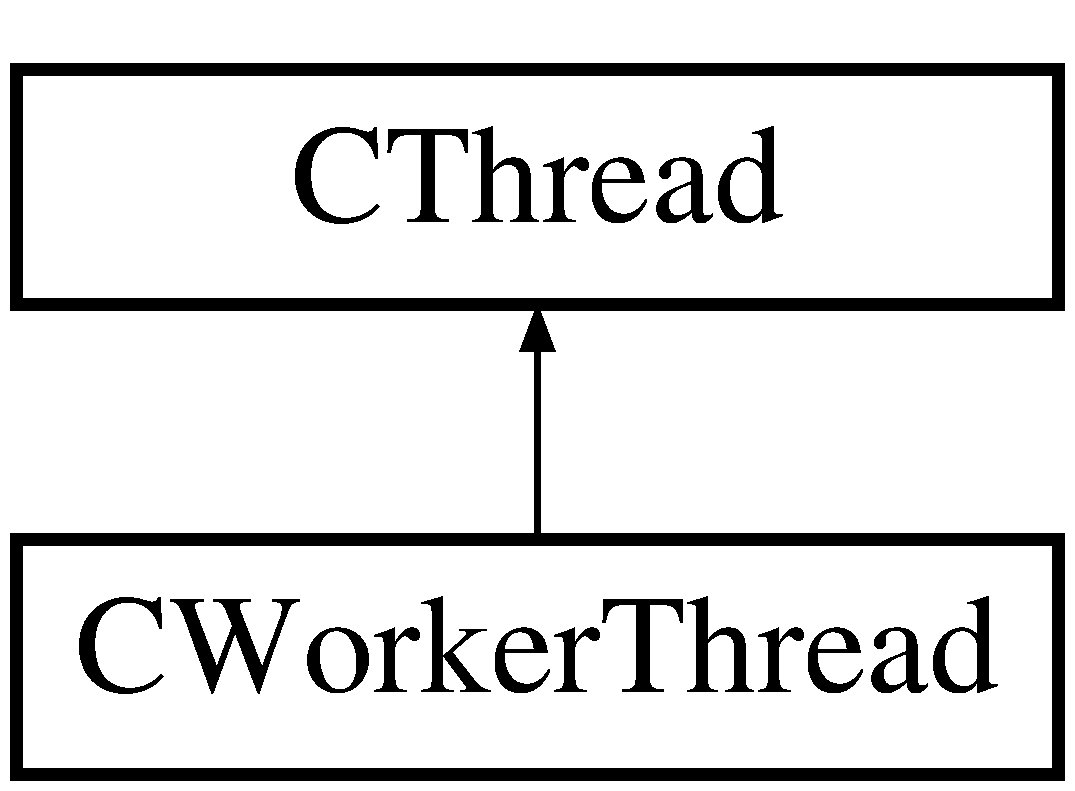
\includegraphics[height=2.000000cm]{class_c_worker_thread}
\end{center}
\end{figure}
\subsection*{公開メンバ関数}
\begin{DoxyCompactItemize}
\item 
\hyperlink{class_c_worker_thread_a2c011a29dc6d6f5c0b40c09ed4f322b2}{C\+Worker\+Thread} (\hyperlink{class_c_worker_channel}{C\+Worker\+Channel} $\ast$\+\_\+pc\+Channel)
\begin{DoxyCompactList}\small\item\em コンストラクタ。 \end{DoxyCompactList}\item 
virtual \hyperlink{class_c_worker_thread_ac48e79f7cc0c6fa81c2600d79142a2d4}{$\sim$\+C\+Worker\+Thread} ()
\begin{DoxyCompactList}\small\item\em デストラクタ。 \end{DoxyCompactList}\item 
virtual void \hyperlink{class_c_worker_thread_ac41c89ce50bb4f499f2d5154a8db5a0f}{Thread\+Callback} () override
\begin{DoxyCompactList}\small\item\em コールバック関数。 \end{DoxyCompactList}\item 
void \hyperlink{class_c_worker_thread_a670abeb8365dc320b291d97e7ea850b2}{Request\+End} ()
\begin{DoxyCompactList}\small\item\em 終了リクエスト。 \end{DoxyCompactList}\item 
bool \hyperlink{class_c_worker_thread_a24c5e2381a0090c85e900558ee0b751a}{Is\+Wait} () const 
\begin{DoxyCompactList}\small\item\em 待機中か。 \end{DoxyCompactList}\end{DoxyCompactItemize}
\subsection*{非公開メンバ関数}
\begin{DoxyCompactItemize}
\item 
void \hyperlink{class_c_worker_thread_a88ea494fd920d5a096dd81cd18ffa5f1}{Set\+Wait} (bool \+\_\+b\+Wait)
\begin{DoxyCompactList}\small\item\em 待機中か設定。 \end{DoxyCompactList}\end{DoxyCompactItemize}
\subsection*{非公開変数類}
\begin{DoxyCompactItemize}
\item 
\hyperlink{class_c_worker_channel}{C\+Worker\+Channel} $\ast$ \hyperlink{class_c_worker_thread_a7168bcaeb8c06da52320dfe49bc4b427}{m\+\_\+pc\+Channel}
\item 
bool \hyperlink{class_c_worker_thread_ac2eeaf5d7a3a74d3b052e8aae18c350c}{m\+\_\+b\+Request\+End}
\item 
bool \hyperlink{class_c_worker_thread_ac692019a76899c582fd0759080108e0b}{m\+\_\+b\+Wait}
\end{DoxyCompactItemize}


\subsection{構築子と解体子}
\hypertarget{class_c_worker_thread_a2c011a29dc6d6f5c0b40c09ed4f322b2}{}\index{C\+Worker\+Thread@{C\+Worker\+Thread}!C\+Worker\+Thread@{C\+Worker\+Thread}}
\index{C\+Worker\+Thread@{C\+Worker\+Thread}!C\+Worker\+Thread@{C\+Worker\+Thread}}
\subsubsection[{C\+Worker\+Thread(\+C\+Worker\+Channel $\ast$\+\_\+pc\+Channel)}]{\setlength{\rightskip}{0pt plus 5cm}C\+Worker\+Thread\+::\+C\+Worker\+Thread (
\begin{DoxyParamCaption}
\item[{{\bf C\+Worker\+Channel} $\ast$}]{\+\_\+pc\+Channel}
\end{DoxyParamCaption}
)}\label{class_c_worker_thread_a2c011a29dc6d6f5c0b40c09ed4f322b2}


コンストラクタ。 


\begin{DoxyParams}{引数}
{\em \+\_\+pc\+Channel} & \+: 仕事の受取元。 \\
\hline
\end{DoxyParams}
\hypertarget{class_c_worker_thread_ac48e79f7cc0c6fa81c2600d79142a2d4}{}\index{C\+Worker\+Thread@{C\+Worker\+Thread}!````~C\+Worker\+Thread@{$\sim$\+C\+Worker\+Thread}}
\index{````~C\+Worker\+Thread@{$\sim$\+C\+Worker\+Thread}!C\+Worker\+Thread@{C\+Worker\+Thread}}
\subsubsection[{$\sim$\+C\+Worker\+Thread()}]{\setlength{\rightskip}{0pt plus 5cm}C\+Worker\+Thread\+::$\sim$\+C\+Worker\+Thread (
\begin{DoxyParamCaption}
{}
\end{DoxyParamCaption}
)\hspace{0.3cm}{\ttfamily [virtual]}}\label{class_c_worker_thread_ac48e79f7cc0c6fa81c2600d79142a2d4}


デストラクタ。 



\subsection{関数詳解}
\hypertarget{class_c_worker_thread_a24c5e2381a0090c85e900558ee0b751a}{}\index{C\+Worker\+Thread@{C\+Worker\+Thread}!Is\+Wait@{Is\+Wait}}
\index{Is\+Wait@{Is\+Wait}!C\+Worker\+Thread@{C\+Worker\+Thread}}
\subsubsection[{Is\+Wait() const }]{\setlength{\rightskip}{0pt plus 5cm}bool C\+Worker\+Thread\+::\+Is\+Wait (
\begin{DoxyParamCaption}
{}
\end{DoxyParamCaption}
) const\hspace{0.3cm}{\ttfamily [inline]}}\label{class_c_worker_thread_a24c5e2381a0090c85e900558ee0b751a}


待機中か。 

\hypertarget{class_c_worker_thread_a670abeb8365dc320b291d97e7ea850b2}{}\index{C\+Worker\+Thread@{C\+Worker\+Thread}!Request\+End@{Request\+End}}
\index{Request\+End@{Request\+End}!C\+Worker\+Thread@{C\+Worker\+Thread}}
\subsubsection[{Request\+End()}]{\setlength{\rightskip}{0pt plus 5cm}void C\+Worker\+Thread\+::\+Request\+End (
\begin{DoxyParamCaption}
{}
\end{DoxyParamCaption}
)\hspace{0.3cm}{\ttfamily [inline]}}\label{class_c_worker_thread_a670abeb8365dc320b291d97e7ea850b2}


終了リクエスト。 

\hypertarget{class_c_worker_thread_a88ea494fd920d5a096dd81cd18ffa5f1}{}\index{C\+Worker\+Thread@{C\+Worker\+Thread}!Set\+Wait@{Set\+Wait}}
\index{Set\+Wait@{Set\+Wait}!C\+Worker\+Thread@{C\+Worker\+Thread}}
\subsubsection[{Set\+Wait(bool \+\_\+b\+Wait)}]{\setlength{\rightskip}{0pt plus 5cm}void C\+Worker\+Thread\+::\+Set\+Wait (
\begin{DoxyParamCaption}
\item[{bool}]{\+\_\+b\+Wait}
\end{DoxyParamCaption}
)\hspace{0.3cm}{\ttfamily [private]}}\label{class_c_worker_thread_a88ea494fd920d5a096dd81cd18ffa5f1}


待機中か設定。 

\hypertarget{class_c_worker_thread_ac41c89ce50bb4f499f2d5154a8db5a0f}{}\index{C\+Worker\+Thread@{C\+Worker\+Thread}!Thread\+Callback@{Thread\+Callback}}
\index{Thread\+Callback@{Thread\+Callback}!C\+Worker\+Thread@{C\+Worker\+Thread}}
\subsubsection[{Thread\+Callback() override}]{\setlength{\rightskip}{0pt plus 5cm}void C\+Worker\+Thread\+::\+Thread\+Callback (
\begin{DoxyParamCaption}
{}
\end{DoxyParamCaption}
)\hspace{0.3cm}{\ttfamily [override]}, {\ttfamily [virtual]}}\label{class_c_worker_thread_ac41c89ce50bb4f499f2d5154a8db5a0f}


コールバック関数。 



\hyperlink{class_c_thread_a15c60ba6d652d92c150fda5e10ebb23e}{C\+Thread}を再実装しています。



\subsection{メンバ詳解}
\hypertarget{class_c_worker_thread_ac2eeaf5d7a3a74d3b052e8aae18c350c}{}\index{C\+Worker\+Thread@{C\+Worker\+Thread}!m\+\_\+b\+Request\+End@{m\+\_\+b\+Request\+End}}
\index{m\+\_\+b\+Request\+End@{m\+\_\+b\+Request\+End}!C\+Worker\+Thread@{C\+Worker\+Thread}}
\subsubsection[{m\+\_\+b\+Request\+End}]{\setlength{\rightskip}{0pt plus 5cm}bool C\+Worker\+Thread\+::m\+\_\+b\+Request\+End\hspace{0.3cm}{\ttfamily [private]}}\label{class_c_worker_thread_ac2eeaf5d7a3a74d3b052e8aae18c350c}
\hypertarget{class_c_worker_thread_ac692019a76899c582fd0759080108e0b}{}\index{C\+Worker\+Thread@{C\+Worker\+Thread}!m\+\_\+b\+Wait@{m\+\_\+b\+Wait}}
\index{m\+\_\+b\+Wait@{m\+\_\+b\+Wait}!C\+Worker\+Thread@{C\+Worker\+Thread}}
\subsubsection[{m\+\_\+b\+Wait}]{\setlength{\rightskip}{0pt plus 5cm}bool C\+Worker\+Thread\+::m\+\_\+b\+Wait\hspace{0.3cm}{\ttfamily [private]}}\label{class_c_worker_thread_ac692019a76899c582fd0759080108e0b}
\hypertarget{class_c_worker_thread_a7168bcaeb8c06da52320dfe49bc4b427}{}\index{C\+Worker\+Thread@{C\+Worker\+Thread}!m\+\_\+pc\+Channel@{m\+\_\+pc\+Channel}}
\index{m\+\_\+pc\+Channel@{m\+\_\+pc\+Channel}!C\+Worker\+Thread@{C\+Worker\+Thread}}
\subsubsection[{m\+\_\+pc\+Channel}]{\setlength{\rightskip}{0pt plus 5cm}{\bf C\+Worker\+Channel}$\ast$ C\+Worker\+Thread\+::m\+\_\+pc\+Channel\hspace{0.3cm}{\ttfamily [private]}}\label{class_c_worker_thread_a7168bcaeb8c06da52320dfe49bc4b427}


このクラス詳解は次のファイルから抽出されました\+:\begin{DoxyCompactItemize}
\item 
D\+:/\+Project/\+Game/\+Lib/\+Worker/\hyperlink{_worker_thread_8h}{Worker\+Thread.\+h}\item 
D\+:/\+Project/\+Game/\+Lib/\+Worker/\hyperlink{_worker_thread_8cpp}{Worker\+Thread.\+cpp}\end{DoxyCompactItemize}

\hypertarget{class_i_constant_buffer}{}\section{I\+Constant\+Buffer クラス}
\label{class_i_constant_buffer}\index{I\+Constant\+Buffer@{I\+Constant\+Buffer}}


{\ttfamily \#include $<$Constant\+Buffer.\+h$>$}

I\+Constant\+Buffer の継承関係図\begin{figure}[H]
\begin{center}
\leavevmode
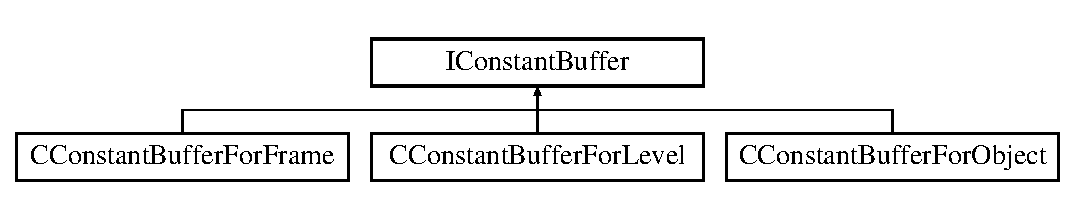
\includegraphics[height=2.000000cm]{class_i_constant_buffer}
\end{center}
\end{figure}
\subsection*{公開メンバ関数}
\begin{DoxyCompactItemize}
\item 
\hyperlink{class_i_constant_buffer_a48109ccf9035a26787b1357f34d4b89f}{I\+Constant\+Buffer} ()
\begin{DoxyCompactList}\small\item\em コンストラクタ。 \end{DoxyCompactList}\item 
virtual \hyperlink{class_i_constant_buffer_a323c41d765bb7d9293d3326b8482b827}{$\sim$\+I\+Constant\+Buffer} ()
\begin{DoxyCompactList}\small\item\em デストラクタ。 \end{DoxyCompactList}\item 
virtual const void $\ast$ \hyperlink{class_i_constant_buffer_a51d7e72f262e74f2018b480102dc795e}{Get\+Data} () const  =0
\begin{DoxyCompactList}\small\item\em コンスタントバッファーにコピーするデータを取得。 \end{DoxyCompactList}\item 
virtual U\+Size \hyperlink{class_i_constant_buffer_a527035ebacd73ffe5c5856f75220ac68}{Get\+Size} () const  =0
\begin{DoxyCompactList}\small\item\em コンスタントバッファーにコピーするデータのサイズを取得。 \end{DoxyCompactList}\end{DoxyCompactItemize}


\subsection{構築子と解体子}
\hypertarget{class_i_constant_buffer_a48109ccf9035a26787b1357f34d4b89f}{}\index{I\+Constant\+Buffer@{I\+Constant\+Buffer}!I\+Constant\+Buffer@{I\+Constant\+Buffer}}
\index{I\+Constant\+Buffer@{I\+Constant\+Buffer}!I\+Constant\+Buffer@{I\+Constant\+Buffer}}
\subsubsection[{I\+Constant\+Buffer()}]{\setlength{\rightskip}{0pt plus 5cm}I\+Constant\+Buffer\+::\+I\+Constant\+Buffer (
\begin{DoxyParamCaption}
{}
\end{DoxyParamCaption}
)\hspace{0.3cm}{\ttfamily [inline]}}\label{class_i_constant_buffer_a48109ccf9035a26787b1357f34d4b89f}


コンストラクタ。 

\hypertarget{class_i_constant_buffer_a323c41d765bb7d9293d3326b8482b827}{}\index{I\+Constant\+Buffer@{I\+Constant\+Buffer}!````~I\+Constant\+Buffer@{$\sim$\+I\+Constant\+Buffer}}
\index{````~I\+Constant\+Buffer@{$\sim$\+I\+Constant\+Buffer}!I\+Constant\+Buffer@{I\+Constant\+Buffer}}
\subsubsection[{$\sim$\+I\+Constant\+Buffer()}]{\setlength{\rightskip}{0pt plus 5cm}virtual I\+Constant\+Buffer\+::$\sim$\+I\+Constant\+Buffer (
\begin{DoxyParamCaption}
{}
\end{DoxyParamCaption}
)\hspace{0.3cm}{\ttfamily [inline]}, {\ttfamily [virtual]}}\label{class_i_constant_buffer_a323c41d765bb7d9293d3326b8482b827}


デストラクタ。 



\subsection{関数詳解}
\hypertarget{class_i_constant_buffer_a51d7e72f262e74f2018b480102dc795e}{}\index{I\+Constant\+Buffer@{I\+Constant\+Buffer}!Get\+Data@{Get\+Data}}
\index{Get\+Data@{Get\+Data}!I\+Constant\+Buffer@{I\+Constant\+Buffer}}
\subsubsection[{Get\+Data() const  =0}]{\setlength{\rightskip}{0pt plus 5cm}virtual const void$\ast$ I\+Constant\+Buffer\+::\+Get\+Data (
\begin{DoxyParamCaption}
{}
\end{DoxyParamCaption}
) const\hspace{0.3cm}{\ttfamily [pure virtual]}}\label{class_i_constant_buffer_a51d7e72f262e74f2018b480102dc795e}


コンスタントバッファーにコピーするデータを取得。 



\hyperlink{class_c_constant_buffer_for_object_aa13289af40c27707fb174a5b3afbdf1b}{C\+Constant\+Buffer\+For\+Object}, \hyperlink{class_c_constant_buffer_for_frame_a1dd7a17aa4584865227d2e4188693da9}{C\+Constant\+Buffer\+For\+Frame}, \hyperlink{class_c_constant_buffer_for_level_a2de25b6e96d4ed77ab5e598389b3bd08}{C\+Constant\+Buffer\+For\+Level}で実装されています。

\hypertarget{class_i_constant_buffer_a527035ebacd73ffe5c5856f75220ac68}{}\index{I\+Constant\+Buffer@{I\+Constant\+Buffer}!Get\+Size@{Get\+Size}}
\index{Get\+Size@{Get\+Size}!I\+Constant\+Buffer@{I\+Constant\+Buffer}}
\subsubsection[{Get\+Size() const  =0}]{\setlength{\rightskip}{0pt plus 5cm}virtual U\+Size I\+Constant\+Buffer\+::\+Get\+Size (
\begin{DoxyParamCaption}
{}
\end{DoxyParamCaption}
) const\hspace{0.3cm}{\ttfamily [pure virtual]}}\label{class_i_constant_buffer_a527035ebacd73ffe5c5856f75220ac68}


コンスタントバッファーにコピーするデータのサイズを取得。 



\hyperlink{class_c_constant_buffer_for_object_a328586af4370d221ada7b270f9f4b8db}{C\+Constant\+Buffer\+For\+Object}, \hyperlink{class_c_constant_buffer_for_frame_afbfb7c7b533d75dc65e01a3f873d6e71}{C\+Constant\+Buffer\+For\+Frame}, \hyperlink{class_c_constant_buffer_for_level_a5d653c0978f370dcef86eece263871dd}{C\+Constant\+Buffer\+For\+Level}で実装されています。



このクラス詳解は次のファイルから抽出されました\+:\begin{DoxyCompactItemize}
\item 
D\+:/\+Project/\+Game/\+Lib/\+Render/\hyperlink{_constant_buffer_8h}{Constant\+Buffer.\+h}\end{DoxyCompactItemize}

\hypertarget{class_i_direct_x_device_factory}{}\section{I\+Direct\+X\+Device\+Factory クラス}
\label{class_i_direct_x_device_factory}\index{I\+Direct\+X\+Device\+Factory@{I\+Direct\+X\+Device\+Factory}}


{\ttfamily \#include $<$Direct\+X\+Device\+Factory.\+h$>$}

\subsection*{公開メンバ関数}
\begin{DoxyCompactItemize}
\item 
\hyperlink{class_i_direct_x_device_factory_a8368fb7bdcfb4b2a20e7522df5089b0d}{I\+Direct\+X\+Device\+Factory} ()
\begin{DoxyCompactList}\small\item\em コンストラクタ。 \end{DoxyCompactList}\item 
virtual \hyperlink{class_i_direct_x_device_factory_afd69636a530417ae42a9970bc97efa07}{$\sim$\+I\+Direct\+X\+Device\+Factory} ()
\begin{DoxyCompactList}\small\item\em デストラクタ。 \end{DoxyCompactList}\item 
virtual I\+D3\+D\+Device $\ast$ \hyperlink{class_i_direct_x_device_factory_ad3d4b3f376b1a8843069de287db990cd}{Create\+Device} ()=0
\begin{DoxyCompactList}\small\item\em デバイスを作成。 \end{DoxyCompactList}\end{DoxyCompactItemize}


\subsection{構築子と解体子}
\hypertarget{class_i_direct_x_device_factory_a8368fb7bdcfb4b2a20e7522df5089b0d}{}\index{I\+Direct\+X\+Device\+Factory@{I\+Direct\+X\+Device\+Factory}!I\+Direct\+X\+Device\+Factory@{I\+Direct\+X\+Device\+Factory}}
\index{I\+Direct\+X\+Device\+Factory@{I\+Direct\+X\+Device\+Factory}!I\+Direct\+X\+Device\+Factory@{I\+Direct\+X\+Device\+Factory}}
\subsubsection[{I\+Direct\+X\+Device\+Factory()}]{\setlength{\rightskip}{0pt plus 5cm}I\+Direct\+X\+Device\+Factory\+::\+I\+Direct\+X\+Device\+Factory (
\begin{DoxyParamCaption}
{}
\end{DoxyParamCaption}
)\hspace{0.3cm}{\ttfamily [inline]}}\label{class_i_direct_x_device_factory_a8368fb7bdcfb4b2a20e7522df5089b0d}


コンストラクタ。 

\hypertarget{class_i_direct_x_device_factory_afd69636a530417ae42a9970bc97efa07}{}\index{I\+Direct\+X\+Device\+Factory@{I\+Direct\+X\+Device\+Factory}!````~I\+Direct\+X\+Device\+Factory@{$\sim$\+I\+Direct\+X\+Device\+Factory}}
\index{````~I\+Direct\+X\+Device\+Factory@{$\sim$\+I\+Direct\+X\+Device\+Factory}!I\+Direct\+X\+Device\+Factory@{I\+Direct\+X\+Device\+Factory}}
\subsubsection[{$\sim$\+I\+Direct\+X\+Device\+Factory()}]{\setlength{\rightskip}{0pt plus 5cm}virtual I\+Direct\+X\+Device\+Factory\+::$\sim$\+I\+Direct\+X\+Device\+Factory (
\begin{DoxyParamCaption}
{}
\end{DoxyParamCaption}
)\hspace{0.3cm}{\ttfamily [inline]}, {\ttfamily [virtual]}}\label{class_i_direct_x_device_factory_afd69636a530417ae42a9970bc97efa07}


デストラクタ。 



\subsection{関数詳解}
\hypertarget{class_i_direct_x_device_factory_ad3d4b3f376b1a8843069de287db990cd}{}\index{I\+Direct\+X\+Device\+Factory@{I\+Direct\+X\+Device\+Factory}!Create\+Device@{Create\+Device}}
\index{Create\+Device@{Create\+Device}!I\+Direct\+X\+Device\+Factory@{I\+Direct\+X\+Device\+Factory}}
\subsubsection[{Create\+Device()=0}]{\setlength{\rightskip}{0pt plus 5cm}virtual I\+D3\+D\+Device$\ast$ I\+Direct\+X\+Device\+Factory\+::\+Create\+Device (
\begin{DoxyParamCaption}
{}
\end{DoxyParamCaption}
)\hspace{0.3cm}{\ttfamily [pure virtual]}}\label{class_i_direct_x_device_factory_ad3d4b3f376b1a8843069de287db990cd}


デバイスを作成。 



このクラス詳解は次のファイルから抽出されました\+:\begin{DoxyCompactItemize}
\item 
D\+:/\+Project/\+Game/\+Lib/\+Direct\+X/\hyperlink{_direct_x_device_factory_8h}{Direct\+X\+Device\+Factory.\+h}\end{DoxyCompactItemize}

\hypertarget{class_i_mesh}{}\section{I\+Mesh クラス}
\label{class_i_mesh}\index{I\+Mesh@{I\+Mesh}}


{\ttfamily \#include $<$Mesh.\+h$>$}

I\+Mesh の継承関係図\begin{figure}[H]
\begin{center}
\leavevmode
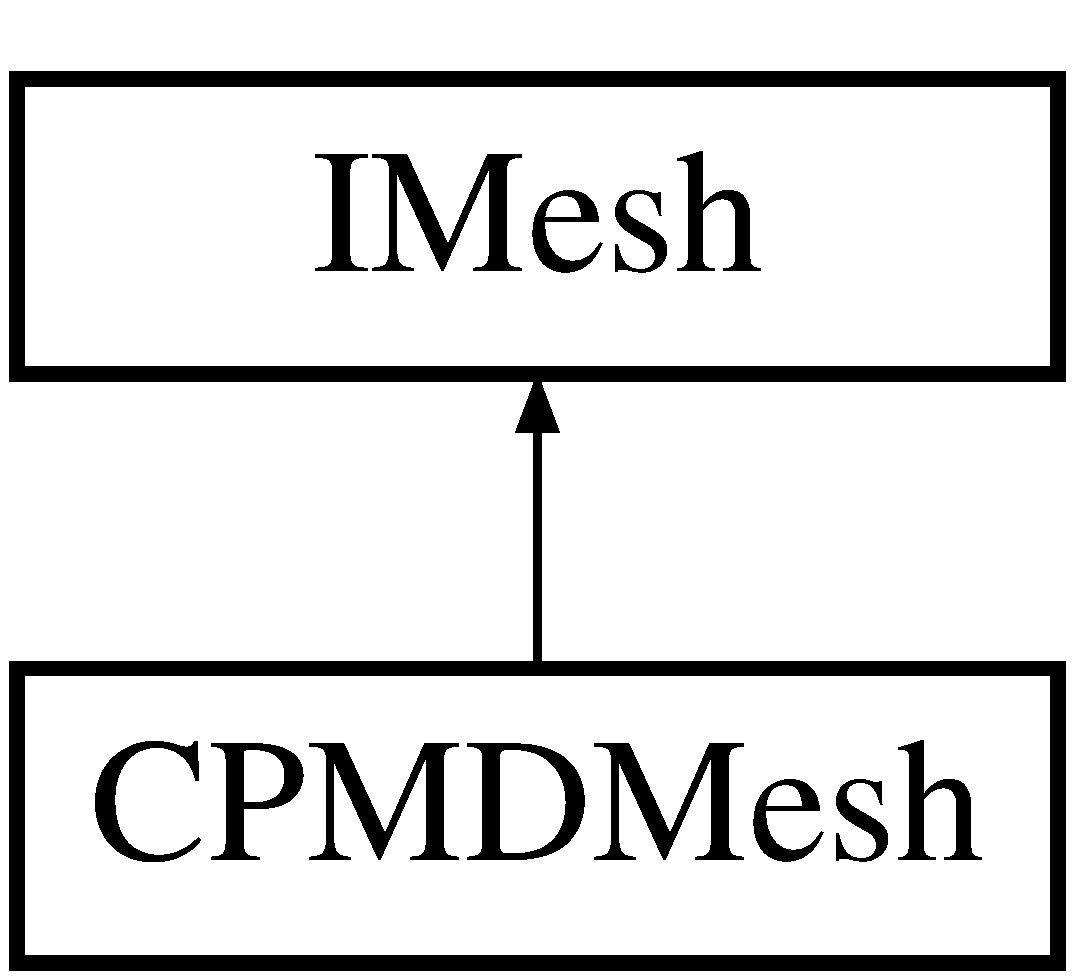
\includegraphics[height=2.000000cm]{class_i_mesh}
\end{center}
\end{figure}
\subsection*{クラス}
\begin{DoxyCompactItemize}
\item 
struct \hyperlink{struct_i_mesh_1_1_st_material}{St\+Material}
\begin{DoxyCompactList}\small\item\em マテリアル情報。 \end{DoxyCompactList}\item 
struct \hyperlink{struct_i_mesh_1_1_st_vertex}{St\+Vertex}
\begin{DoxyCompactList}\small\item\em 頂点情報。 \end{DoxyCompactList}\end{DoxyCompactItemize}
\subsection*{公開メンバ関数}
\begin{DoxyCompactItemize}
\item 
\hyperlink{class_i_mesh_a39bf278a127fe4a317c53e8e0dd66d32}{I\+Mesh} ()
\begin{DoxyCompactList}\small\item\em コンストラクタ。 \end{DoxyCompactList}\item 
virtual \hyperlink{class_i_mesh_a1227ad691cc829ef540b3ff956019423}{$\sim$\+I\+Mesh} ()
\begin{DoxyCompactList}\small\item\em デストラクタ。 \end{DoxyCompactList}\item 
virtual U32 \hyperlink{class_i_mesh_a98ac2c9b1da3c22191e4198833a4f6ef}{Get\+Vertex\+Num} () const  =0
\begin{DoxyCompactList}\small\item\em 頂点情報数を取得。 \end{DoxyCompactList}\item 
virtual const \hyperlink{struct_i_mesh_1_1_st_vertex}{St\+Vertex} $\ast$ \hyperlink{class_i_mesh_a91d4b99a5a91cb54d364cc6a8342b187}{Get\+Vertex\+Array} () const  =0
\begin{DoxyCompactList}\small\item\em 頂点情報配列を取得。 \end{DoxyCompactList}\item 
virtual U32 \hyperlink{class_i_mesh_a580358c71d8766c1e0aa8037b51a9296}{Get\+Index\+Num} () const  =0
\begin{DoxyCompactList}\small\item\em インデックス数を取得。 \end{DoxyCompactList}\item 
virtual const U32 $\ast$ \hyperlink{class_i_mesh_a3a9e9207cfae24ae1dd62eb2d2356301}{Get\+Index\+Array} () const  =0
\begin{DoxyCompactList}\small\item\em インデックス配列を取得。 \end{DoxyCompactList}\item 
virtual U32 \hyperlink{class_i_mesh_a1b8922bc90cd0951062053e24287ad6c}{Get\+Material\+Num} () const  =0
\begin{DoxyCompactList}\small\item\em マテリアル数を取得。 \end{DoxyCompactList}\item 
virtual const \hyperlink{struct_i_mesh_1_1_st_material}{St\+Material} $\ast$ \hyperlink{class_i_mesh_a48afb85120e333b50ac9de73b8b60d16}{Get\+Material\+Array} () const  =0
\begin{DoxyCompactList}\small\item\em マテリアル配列を取得。 \end{DoxyCompactList}\end{DoxyCompactItemize}


\subsection{構築子と解体子}
\hypertarget{class_i_mesh_a39bf278a127fe4a317c53e8e0dd66d32}{}\index{I\+Mesh@{I\+Mesh}!I\+Mesh@{I\+Mesh}}
\index{I\+Mesh@{I\+Mesh}!I\+Mesh@{I\+Mesh}}
\subsubsection[{I\+Mesh()}]{\setlength{\rightskip}{0pt plus 5cm}I\+Mesh\+::\+I\+Mesh (
\begin{DoxyParamCaption}
{}
\end{DoxyParamCaption}
)\hspace{0.3cm}{\ttfamily [inline]}}\label{class_i_mesh_a39bf278a127fe4a317c53e8e0dd66d32}


コンストラクタ。 

\hypertarget{class_i_mesh_a1227ad691cc829ef540b3ff956019423}{}\index{I\+Mesh@{I\+Mesh}!````~I\+Mesh@{$\sim$\+I\+Mesh}}
\index{````~I\+Mesh@{$\sim$\+I\+Mesh}!I\+Mesh@{I\+Mesh}}
\subsubsection[{$\sim$\+I\+Mesh()}]{\setlength{\rightskip}{0pt plus 5cm}virtual I\+Mesh\+::$\sim$\+I\+Mesh (
\begin{DoxyParamCaption}
{}
\end{DoxyParamCaption}
)\hspace{0.3cm}{\ttfamily [inline]}, {\ttfamily [virtual]}}\label{class_i_mesh_a1227ad691cc829ef540b3ff956019423}


デストラクタ。 



\subsection{関数詳解}
\hypertarget{class_i_mesh_a3a9e9207cfae24ae1dd62eb2d2356301}{}\index{I\+Mesh@{I\+Mesh}!Get\+Index\+Array@{Get\+Index\+Array}}
\index{Get\+Index\+Array@{Get\+Index\+Array}!I\+Mesh@{I\+Mesh}}
\subsubsection[{Get\+Index\+Array() const  =0}]{\setlength{\rightskip}{0pt plus 5cm}virtual const U32$\ast$ I\+Mesh\+::\+Get\+Index\+Array (
\begin{DoxyParamCaption}
{}
\end{DoxyParamCaption}
) const\hspace{0.3cm}{\ttfamily [pure virtual]}}\label{class_i_mesh_a3a9e9207cfae24ae1dd62eb2d2356301}


インデックス配列を取得。 



\hyperlink{class_c_p_m_d_mesh_ab2b12b75b3ed1ed3017cff8d52f1677b}{C\+P\+M\+D\+Mesh}で実装されています。

\hypertarget{class_i_mesh_a580358c71d8766c1e0aa8037b51a9296}{}\index{I\+Mesh@{I\+Mesh}!Get\+Index\+Num@{Get\+Index\+Num}}
\index{Get\+Index\+Num@{Get\+Index\+Num}!I\+Mesh@{I\+Mesh}}
\subsubsection[{Get\+Index\+Num() const  =0}]{\setlength{\rightskip}{0pt plus 5cm}virtual U32 I\+Mesh\+::\+Get\+Index\+Num (
\begin{DoxyParamCaption}
{}
\end{DoxyParamCaption}
) const\hspace{0.3cm}{\ttfamily [pure virtual]}}\label{class_i_mesh_a580358c71d8766c1e0aa8037b51a9296}


インデックス数を取得。 



\hyperlink{class_c_p_m_d_mesh_a0127281ef228e27dd6232069c5ffd164}{C\+P\+M\+D\+Mesh}で実装されています。

\hypertarget{class_i_mesh_a48afb85120e333b50ac9de73b8b60d16}{}\index{I\+Mesh@{I\+Mesh}!Get\+Material\+Array@{Get\+Material\+Array}}
\index{Get\+Material\+Array@{Get\+Material\+Array}!I\+Mesh@{I\+Mesh}}
\subsubsection[{Get\+Material\+Array() const  =0}]{\setlength{\rightskip}{0pt plus 5cm}virtual const {\bf St\+Material}$\ast$ I\+Mesh\+::\+Get\+Material\+Array (
\begin{DoxyParamCaption}
{}
\end{DoxyParamCaption}
) const\hspace{0.3cm}{\ttfamily [pure virtual]}}\label{class_i_mesh_a48afb85120e333b50ac9de73b8b60d16}


マテリアル配列を取得。 



\hyperlink{class_c_p_m_d_mesh_a8b6ba1255586f2387442ec24f92ade55}{C\+P\+M\+D\+Mesh}で実装されています。

\hypertarget{class_i_mesh_a1b8922bc90cd0951062053e24287ad6c}{}\index{I\+Mesh@{I\+Mesh}!Get\+Material\+Num@{Get\+Material\+Num}}
\index{Get\+Material\+Num@{Get\+Material\+Num}!I\+Mesh@{I\+Mesh}}
\subsubsection[{Get\+Material\+Num() const  =0}]{\setlength{\rightskip}{0pt plus 5cm}virtual U32 I\+Mesh\+::\+Get\+Material\+Num (
\begin{DoxyParamCaption}
{}
\end{DoxyParamCaption}
) const\hspace{0.3cm}{\ttfamily [pure virtual]}}\label{class_i_mesh_a1b8922bc90cd0951062053e24287ad6c}


マテリアル数を取得。 



\hyperlink{class_c_p_m_d_mesh_a3dc32e47f692de7cc2c998b65a416c6d}{C\+P\+M\+D\+Mesh}で実装されています。

\hypertarget{class_i_mesh_a91d4b99a5a91cb54d364cc6a8342b187}{}\index{I\+Mesh@{I\+Mesh}!Get\+Vertex\+Array@{Get\+Vertex\+Array}}
\index{Get\+Vertex\+Array@{Get\+Vertex\+Array}!I\+Mesh@{I\+Mesh}}
\subsubsection[{Get\+Vertex\+Array() const  =0}]{\setlength{\rightskip}{0pt plus 5cm}virtual const {\bf St\+Vertex}$\ast$ I\+Mesh\+::\+Get\+Vertex\+Array (
\begin{DoxyParamCaption}
{}
\end{DoxyParamCaption}
) const\hspace{0.3cm}{\ttfamily [pure virtual]}}\label{class_i_mesh_a91d4b99a5a91cb54d364cc6a8342b187}


頂点情報配列を取得。 



\hyperlink{class_c_p_m_d_mesh_aa2b096b1102286fec5d8ea7cc381bb55}{C\+P\+M\+D\+Mesh}で実装されています。

\hypertarget{class_i_mesh_a98ac2c9b1da3c22191e4198833a4f6ef}{}\index{I\+Mesh@{I\+Mesh}!Get\+Vertex\+Num@{Get\+Vertex\+Num}}
\index{Get\+Vertex\+Num@{Get\+Vertex\+Num}!I\+Mesh@{I\+Mesh}}
\subsubsection[{Get\+Vertex\+Num() const  =0}]{\setlength{\rightskip}{0pt plus 5cm}virtual U32 I\+Mesh\+::\+Get\+Vertex\+Num (
\begin{DoxyParamCaption}
{}
\end{DoxyParamCaption}
) const\hspace{0.3cm}{\ttfamily [pure virtual]}}\label{class_i_mesh_a98ac2c9b1da3c22191e4198833a4f6ef}


頂点情報数を取得。 



\hyperlink{class_c_p_m_d_mesh_a99a0e4d3664fae495cfe216170294aab}{C\+P\+M\+D\+Mesh}で実装されています。



このクラス詳解は次のファイルから抽出されました\+:\begin{DoxyCompactItemize}
\item 
D\+:/\+Project/\+Game/\+Lib/\+Mesh/\hyperlink{_mesh_8h}{Mesh.\+h}\end{DoxyCompactItemize}

\hypertarget{class_i_render_context}{}\section{I\+Render\+Context クラス}
\label{class_i_render_context}\index{I\+Render\+Context@{I\+Render\+Context}}


{\ttfamily \#include $<$Render\+Context.\+h$>$}

\subsection*{公開メンバ関数}
\begin{DoxyCompactItemize}
\item 
virtual \hyperlink{class_i_render_context_a1c20807e9f3706873a9d7f49bf4fe43f}{$\sim$\+I\+Render\+Context} ()
\begin{DoxyCompactList}\small\item\em デストラクタ。 \end{DoxyCompactList}\item 
virtual void \hyperlink{class_i_render_context_a4e2185c38b1599cf94f52c99d2a8b9fc}{Render} ()=0
\begin{DoxyCompactList}\small\item\em 描画。 \end{DoxyCompactList}\item 
virtual void \hyperlink{class_i_render_context_af39a3637d8844d1728ea7363673525d6}{Clear} ()=0
\begin{DoxyCompactList}\small\item\em 画面のクリア。 \end{DoxyCompactList}\item 
virtual void \hyperlink{class_i_render_context_acab012460a88d3d4df1115fcbd0d553e}{Set\+Constant\+Buffer} (\hyperlink{_constant_buffer_8h_aaf416c55b2e43195b9cf771071e1328a}{En\+Constant\+Buffer} \+\_\+e\+Kind, \hyperlink{class_i_constant_buffer}{I\+Constant\+Buffer} $\ast$\+\_\+pc\+Constant\+Buffer)=0
\begin{DoxyCompactList}\small\item\em コンスタントバッファーの設定。 \end{DoxyCompactList}\end{DoxyCompactItemize}


\subsection{構築子と解体子}
\hypertarget{class_i_render_context_a1c20807e9f3706873a9d7f49bf4fe43f}{}\index{I\+Render\+Context@{I\+Render\+Context}!````~I\+Render\+Context@{$\sim$\+I\+Render\+Context}}
\index{````~I\+Render\+Context@{$\sim$\+I\+Render\+Context}!I\+Render\+Context@{I\+Render\+Context}}
\subsubsection[{$\sim$\+I\+Render\+Context()}]{\setlength{\rightskip}{0pt plus 5cm}virtual I\+Render\+Context\+::$\sim$\+I\+Render\+Context (
\begin{DoxyParamCaption}
{}
\end{DoxyParamCaption}
)\hspace{0.3cm}{\ttfamily [inline]}, {\ttfamily [virtual]}}\label{class_i_render_context_a1c20807e9f3706873a9d7f49bf4fe43f}


デストラクタ。 



\subsection{関数詳解}
\hypertarget{class_i_render_context_af39a3637d8844d1728ea7363673525d6}{}\index{I\+Render\+Context@{I\+Render\+Context}!Clear@{Clear}}
\index{Clear@{Clear}!I\+Render\+Context@{I\+Render\+Context}}
\subsubsection[{Clear()=0}]{\setlength{\rightskip}{0pt plus 5cm}virtual void I\+Render\+Context\+::\+Clear (
\begin{DoxyParamCaption}
{}
\end{DoxyParamCaption}
)\hspace{0.3cm}{\ttfamily [pure virtual]}}\label{class_i_render_context_af39a3637d8844d1728ea7363673525d6}


画面のクリア。 

\hypertarget{class_i_render_context_a4e2185c38b1599cf94f52c99d2a8b9fc}{}\index{I\+Render\+Context@{I\+Render\+Context}!Render@{Render}}
\index{Render@{Render}!I\+Render\+Context@{I\+Render\+Context}}
\subsubsection[{Render()=0}]{\setlength{\rightskip}{0pt plus 5cm}virtual void I\+Render\+Context\+::\+Render (
\begin{DoxyParamCaption}
{}
\end{DoxyParamCaption}
)\hspace{0.3cm}{\ttfamily [pure virtual]}}\label{class_i_render_context_a4e2185c38b1599cf94f52c99d2a8b9fc}


描画。 

\hypertarget{class_i_render_context_acab012460a88d3d4df1115fcbd0d553e}{}\index{I\+Render\+Context@{I\+Render\+Context}!Set\+Constant\+Buffer@{Set\+Constant\+Buffer}}
\index{Set\+Constant\+Buffer@{Set\+Constant\+Buffer}!I\+Render\+Context@{I\+Render\+Context}}
\subsubsection[{Set\+Constant\+Buffer(\+En\+Constant\+Buffer \+\_\+e\+Kind, I\+Constant\+Buffer $\ast$\+\_\+pc\+Constant\+Buffer)=0}]{\setlength{\rightskip}{0pt plus 5cm}virtual void I\+Render\+Context\+::\+Set\+Constant\+Buffer (
\begin{DoxyParamCaption}
\item[{{\bf En\+Constant\+Buffer}}]{\+\_\+e\+Kind, }
\item[{{\bf I\+Constant\+Buffer} $\ast$}]{\+\_\+pc\+Constant\+Buffer}
\end{DoxyParamCaption}
)\hspace{0.3cm}{\ttfamily [pure virtual]}}\label{class_i_render_context_acab012460a88d3d4df1115fcbd0d553e}


コンスタントバッファーの設定。 



このクラス詳解は次のファイルから抽出されました\+:\begin{DoxyCompactItemize}
\item 
D\+:/\+Project/\+Game/\+Lib/\+Render/\hyperlink{_render_context_8h}{Render\+Context.\+h}\end{DoxyCompactItemize}

\hypertarget{class_i_render_context_factory}{}\section{I\+Render\+Context\+Factory クラス}
\label{class_i_render_context_factory}\index{I\+Render\+Context\+Factory@{I\+Render\+Context\+Factory}}


{\ttfamily \#include $<$Render\+Context\+Factory.\+h$>$}

\subsection*{公開メンバ関数}
\begin{DoxyCompactItemize}
\item 
\hyperlink{class_i_render_context_factory_a4df042974217f5d1efbe74b69777abf9}{I\+Render\+Context\+Factory} ()
\begin{DoxyCompactList}\small\item\em コンストラクタ。 \end{DoxyCompactList}\item 
virtual \hyperlink{class_i_render_context_factory_a8098f06bb38f1d4d955d62449534a682}{$\sim$\+I\+Render\+Context\+Factory} ()
\begin{DoxyCompactList}\small\item\em デストラクタ。 \end{DoxyCompactList}\item 
virtual \hyperlink{class_i_render_context}{I\+Render\+Context} $\ast$ \hyperlink{class_i_render_context_factory_a09a8e1e982f451cd407521894a4ae719}{Create} ()=0
\begin{DoxyCompactList}\small\item\em 生成。 \end{DoxyCompactList}\end{DoxyCompactItemize}


\subsection{構築子と解体子}
\hypertarget{class_i_render_context_factory_a4df042974217f5d1efbe74b69777abf9}{}\index{I\+Render\+Context\+Factory@{I\+Render\+Context\+Factory}!I\+Render\+Context\+Factory@{I\+Render\+Context\+Factory}}
\index{I\+Render\+Context\+Factory@{I\+Render\+Context\+Factory}!I\+Render\+Context\+Factory@{I\+Render\+Context\+Factory}}
\subsubsection[{I\+Render\+Context\+Factory()}]{\setlength{\rightskip}{0pt plus 5cm}I\+Render\+Context\+Factory\+::\+I\+Render\+Context\+Factory (
\begin{DoxyParamCaption}
{}
\end{DoxyParamCaption}
)\hspace{0.3cm}{\ttfamily [inline]}}\label{class_i_render_context_factory_a4df042974217f5d1efbe74b69777abf9}


コンストラクタ。 

\hypertarget{class_i_render_context_factory_a8098f06bb38f1d4d955d62449534a682}{}\index{I\+Render\+Context\+Factory@{I\+Render\+Context\+Factory}!````~I\+Render\+Context\+Factory@{$\sim$\+I\+Render\+Context\+Factory}}
\index{````~I\+Render\+Context\+Factory@{$\sim$\+I\+Render\+Context\+Factory}!I\+Render\+Context\+Factory@{I\+Render\+Context\+Factory}}
\subsubsection[{$\sim$\+I\+Render\+Context\+Factory()}]{\setlength{\rightskip}{0pt plus 5cm}virtual I\+Render\+Context\+Factory\+::$\sim$\+I\+Render\+Context\+Factory (
\begin{DoxyParamCaption}
{}
\end{DoxyParamCaption}
)\hspace{0.3cm}{\ttfamily [inline]}, {\ttfamily [virtual]}}\label{class_i_render_context_factory_a8098f06bb38f1d4d955d62449534a682}


デストラクタ。 



\subsection{関数詳解}
\hypertarget{class_i_render_context_factory_a09a8e1e982f451cd407521894a4ae719}{}\index{I\+Render\+Context\+Factory@{I\+Render\+Context\+Factory}!Create@{Create}}
\index{Create@{Create}!I\+Render\+Context\+Factory@{I\+Render\+Context\+Factory}}
\subsubsection[{Create()=0}]{\setlength{\rightskip}{0pt plus 5cm}virtual {\bf I\+Render\+Context}$\ast$ I\+Render\+Context\+Factory\+::\+Create (
\begin{DoxyParamCaption}
{}
\end{DoxyParamCaption}
)\hspace{0.3cm}{\ttfamily [pure virtual]}}\label{class_i_render_context_factory_a09a8e1e982f451cd407521894a4ae719}


生成。 



このクラス詳解は次のファイルから抽出されました\+:\begin{DoxyCompactItemize}
\item 
D\+:/\+Project/\+Game/\+Lib/\+Render/\hyperlink{_render_context_factory_8h}{Render\+Context\+Factory.\+h}\end{DoxyCompactItemize}

\hypertarget{struct_c_allocator_1_1rebind}{}\section{C\+Allocator$<$ T $>$\+:\+:rebind$<$ U $>$ 構造体テンプレート}
\label{struct_c_allocator_1_1rebind}\index{C\+Allocator$<$ T $>$\+::rebind$<$ U $>$@{C\+Allocator$<$ T $>$\+::rebind$<$ U $>$}}


{\ttfamily \#include $<$Allocator.\+h$>$}

\subsection*{公開型}
\begin{DoxyCompactItemize}
\item 
typedef \hyperlink{class_c_allocator}{C\+Allocator}$<$ U $>$ \hyperlink{struct_c_allocator_1_1rebind_a5109d5245fdca0ac2c912fde83828d1d}{other}
\end{DoxyCompactItemize}


\subsection{型定義メンバ詳解}
\hypertarget{struct_c_allocator_1_1rebind_a5109d5245fdca0ac2c912fde83828d1d}{}\index{C\+Allocator\+::rebind@{C\+Allocator\+::rebind}!other@{other}}
\index{other@{other}!C\+Allocator\+::rebind@{C\+Allocator\+::rebind}}
\subsubsection[{other}]{\setlength{\rightskip}{0pt plus 5cm}template$<$class T$>$ template$<$class U $>$ typedef {\bf C\+Allocator}$<$U$>$ {\bf C\+Allocator}$<$ T $>$\+::{\bf rebind}$<$ U $>$\+::{\bf other}}\label{struct_c_allocator_1_1rebind_a5109d5245fdca0ac2c912fde83828d1d}


この構造体詳解は次のファイルから抽出されました\+:\begin{DoxyCompactItemize}
\item 
D\+:/\+Project/\+Game/\+Lib/\+Memory/\+Allocator/\hyperlink{_allocator_8h}{Allocator.\+h}\end{DoxyCompactItemize}

\hypertarget{struct_c_constant_buffer_for_object_1_1_st_constant_buffer}{}\section{C\+Constant\+Buffer\+For\+Object\+:\+:St\+Constant\+Buffer 構造体}
\label{struct_c_constant_buffer_for_object_1_1_st_constant_buffer}\index{C\+Constant\+Buffer\+For\+Object\+::\+St\+Constant\+Buffer@{C\+Constant\+Buffer\+For\+Object\+::\+St\+Constant\+Buffer}}


コンスタントバッファー構造体。  




{\ttfamily \#include $<$Constant\+Buffer\+For\+Object.\+h$>$}

\subsection*{公開メンバ関数}
\begin{DoxyCompactItemize}
\item 
void \hyperlink{struct_c_constant_buffer_for_object_1_1_st_constant_buffer_afc161d34c410eff7479fde11c9350374}{Init} ()
\end{DoxyCompactItemize}
\subsection*{公開変数類}
\begin{DoxyCompactItemize}
\item 
\hyperlink{struct_st_matrix}{St\+Matrix}$<$ F32 $>$ \hyperlink{struct_c_constant_buffer_for_object_1_1_st_constant_buffer_ad9f4abda99ca8f74484d3b965dea439b}{m\+\_\+st\+Mtx\+World}
\item 
\hyperlink{struct_st_matrix}{St\+Matrix}$<$ F32 $>$ \hyperlink{struct_c_constant_buffer_for_object_1_1_st_constant_buffer_a60dc78875ce1e9c5864de6b95dea49d9}{m\+\_\+st\+Mtx\+View}
\item 
\hyperlink{struct_st_matrix}{St\+Matrix}$<$ F32 $>$ \hyperlink{struct_c_constant_buffer_for_object_1_1_st_constant_buffer_adbff5690d0878dd28ee24a2806cbd054}{m\+\_\+st\+Mtx\+Projection}
\end{DoxyCompactItemize}


\subsection{詳解}
コンスタントバッファー構造体。 

\subsection{関数詳解}
\hypertarget{struct_c_constant_buffer_for_object_1_1_st_constant_buffer_afc161d34c410eff7479fde11c9350374}{}\index{C\+Constant\+Buffer\+For\+Object\+::\+St\+Constant\+Buffer@{C\+Constant\+Buffer\+For\+Object\+::\+St\+Constant\+Buffer}!Init@{Init}}
\index{Init@{Init}!C\+Constant\+Buffer\+For\+Object\+::\+St\+Constant\+Buffer@{C\+Constant\+Buffer\+For\+Object\+::\+St\+Constant\+Buffer}}
\subsubsection[{Init()}]{\setlength{\rightskip}{0pt plus 5cm}void C\+Constant\+Buffer\+For\+Object\+::\+St\+Constant\+Buffer\+::\+Init (
\begin{DoxyParamCaption}
{}
\end{DoxyParamCaption}
)\hspace{0.3cm}{\ttfamily [inline]}}\label{struct_c_constant_buffer_for_object_1_1_st_constant_buffer_afc161d34c410eff7479fde11c9350374}


\subsection{メンバ詳解}
\hypertarget{struct_c_constant_buffer_for_object_1_1_st_constant_buffer_adbff5690d0878dd28ee24a2806cbd054}{}\index{C\+Constant\+Buffer\+For\+Object\+::\+St\+Constant\+Buffer@{C\+Constant\+Buffer\+For\+Object\+::\+St\+Constant\+Buffer}!m\+\_\+st\+Mtx\+Projection@{m\+\_\+st\+Mtx\+Projection}}
\index{m\+\_\+st\+Mtx\+Projection@{m\+\_\+st\+Mtx\+Projection}!C\+Constant\+Buffer\+For\+Object\+::\+St\+Constant\+Buffer@{C\+Constant\+Buffer\+For\+Object\+::\+St\+Constant\+Buffer}}
\subsubsection[{m\+\_\+st\+Mtx\+Projection}]{\setlength{\rightskip}{0pt plus 5cm}{\bf St\+Matrix}$<$F32$>$ C\+Constant\+Buffer\+For\+Object\+::\+St\+Constant\+Buffer\+::m\+\_\+st\+Mtx\+Projection}\label{struct_c_constant_buffer_for_object_1_1_st_constant_buffer_adbff5690d0878dd28ee24a2806cbd054}
\hypertarget{struct_c_constant_buffer_for_object_1_1_st_constant_buffer_a60dc78875ce1e9c5864de6b95dea49d9}{}\index{C\+Constant\+Buffer\+For\+Object\+::\+St\+Constant\+Buffer@{C\+Constant\+Buffer\+For\+Object\+::\+St\+Constant\+Buffer}!m\+\_\+st\+Mtx\+View@{m\+\_\+st\+Mtx\+View}}
\index{m\+\_\+st\+Mtx\+View@{m\+\_\+st\+Mtx\+View}!C\+Constant\+Buffer\+For\+Object\+::\+St\+Constant\+Buffer@{C\+Constant\+Buffer\+For\+Object\+::\+St\+Constant\+Buffer}}
\subsubsection[{m\+\_\+st\+Mtx\+View}]{\setlength{\rightskip}{0pt plus 5cm}{\bf St\+Matrix}$<$F32$>$ C\+Constant\+Buffer\+For\+Object\+::\+St\+Constant\+Buffer\+::m\+\_\+st\+Mtx\+View}\label{struct_c_constant_buffer_for_object_1_1_st_constant_buffer_a60dc78875ce1e9c5864de6b95dea49d9}
\hypertarget{struct_c_constant_buffer_for_object_1_1_st_constant_buffer_ad9f4abda99ca8f74484d3b965dea439b}{}\index{C\+Constant\+Buffer\+For\+Object\+::\+St\+Constant\+Buffer@{C\+Constant\+Buffer\+For\+Object\+::\+St\+Constant\+Buffer}!m\+\_\+st\+Mtx\+World@{m\+\_\+st\+Mtx\+World}}
\index{m\+\_\+st\+Mtx\+World@{m\+\_\+st\+Mtx\+World}!C\+Constant\+Buffer\+For\+Object\+::\+St\+Constant\+Buffer@{C\+Constant\+Buffer\+For\+Object\+::\+St\+Constant\+Buffer}}
\subsubsection[{m\+\_\+st\+Mtx\+World}]{\setlength{\rightskip}{0pt plus 5cm}{\bf St\+Matrix}$<$F32$>$ C\+Constant\+Buffer\+For\+Object\+::\+St\+Constant\+Buffer\+::m\+\_\+st\+Mtx\+World}\label{struct_c_constant_buffer_for_object_1_1_st_constant_buffer_ad9f4abda99ca8f74484d3b965dea439b}


この構造体詳解は次のファイルから抽出されました\+:\begin{DoxyCompactItemize}
\item 
D\+:/\+Project/\+Game/\+Lib/\+Render/\hyperlink{_constant_buffer_for_object_8h}{Constant\+Buffer\+For\+Object.\+h}\end{DoxyCompactItemize}

\hypertarget{struct_c_constant_buffer_for_level_1_1_st_constant_buffer}{}\section{C\+Constant\+Buffer\+For\+Level\+:\+:St\+Constant\+Buffer 構造体}
\label{struct_c_constant_buffer_for_level_1_1_st_constant_buffer}\index{C\+Constant\+Buffer\+For\+Level\+::\+St\+Constant\+Buffer@{C\+Constant\+Buffer\+For\+Level\+::\+St\+Constant\+Buffer}}


コンスタントバッファー構造体。  




{\ttfamily \#include $<$Constant\+Buffer\+For\+Level.\+h$>$}

\subsection*{公開メンバ関数}
\begin{DoxyCompactItemize}
\item 
void \hyperlink{struct_c_constant_buffer_for_level_1_1_st_constant_buffer_ac4cf0fbf8e8fa5b757ba3176c97c29a4}{Init} ()
\end{DoxyCompactItemize}
\subsection*{公開変数類}
\begin{DoxyCompactItemize}
\item 
\hyperlink{struct_st_matrix}{St\+Matrix}$<$ F32 $>$ \hyperlink{struct_c_constant_buffer_for_level_1_1_st_constant_buffer_a0f47f708a3588edd70482c2517a80457}{m\+\_\+st\+Mtx\+Dummy}
\end{DoxyCompactItemize}


\subsection{詳解}
コンスタントバッファー構造体。 

\subsection{関数詳解}
\hypertarget{struct_c_constant_buffer_for_level_1_1_st_constant_buffer_ac4cf0fbf8e8fa5b757ba3176c97c29a4}{}\index{C\+Constant\+Buffer\+For\+Level\+::\+St\+Constant\+Buffer@{C\+Constant\+Buffer\+For\+Level\+::\+St\+Constant\+Buffer}!Init@{Init}}
\index{Init@{Init}!C\+Constant\+Buffer\+For\+Level\+::\+St\+Constant\+Buffer@{C\+Constant\+Buffer\+For\+Level\+::\+St\+Constant\+Buffer}}
\subsubsection[{Init()}]{\setlength{\rightskip}{0pt plus 5cm}void C\+Constant\+Buffer\+For\+Level\+::\+St\+Constant\+Buffer\+::\+Init (
\begin{DoxyParamCaption}
{}
\end{DoxyParamCaption}
)\hspace{0.3cm}{\ttfamily [inline]}}\label{struct_c_constant_buffer_for_level_1_1_st_constant_buffer_ac4cf0fbf8e8fa5b757ba3176c97c29a4}


\subsection{メンバ詳解}
\hypertarget{struct_c_constant_buffer_for_level_1_1_st_constant_buffer_a0f47f708a3588edd70482c2517a80457}{}\index{C\+Constant\+Buffer\+For\+Level\+::\+St\+Constant\+Buffer@{C\+Constant\+Buffer\+For\+Level\+::\+St\+Constant\+Buffer}!m\+\_\+st\+Mtx\+Dummy@{m\+\_\+st\+Mtx\+Dummy}}
\index{m\+\_\+st\+Mtx\+Dummy@{m\+\_\+st\+Mtx\+Dummy}!C\+Constant\+Buffer\+For\+Level\+::\+St\+Constant\+Buffer@{C\+Constant\+Buffer\+For\+Level\+::\+St\+Constant\+Buffer}}
\subsubsection[{m\+\_\+st\+Mtx\+Dummy}]{\setlength{\rightskip}{0pt plus 5cm}{\bf St\+Matrix}$<$F32$>$ C\+Constant\+Buffer\+For\+Level\+::\+St\+Constant\+Buffer\+::m\+\_\+st\+Mtx\+Dummy}\label{struct_c_constant_buffer_for_level_1_1_st_constant_buffer_a0f47f708a3588edd70482c2517a80457}


この構造体詳解は次のファイルから抽出されました\+:\begin{DoxyCompactItemize}
\item 
D\+:/\+Project/\+Game/\+Lib/\+Render/\hyperlink{_constant_buffer_for_level_8h}{Constant\+Buffer\+For\+Level.\+h}\end{DoxyCompactItemize}

\hypertarget{struct_c_constant_buffer_for_frame_1_1_st_constant_buffer}{}\section{C\+Constant\+Buffer\+For\+Frame\+:\+:St\+Constant\+Buffer 構造体}
\label{struct_c_constant_buffer_for_frame_1_1_st_constant_buffer}\index{C\+Constant\+Buffer\+For\+Frame\+::\+St\+Constant\+Buffer@{C\+Constant\+Buffer\+For\+Frame\+::\+St\+Constant\+Buffer}}


コンスタントバッファー構造体。  




{\ttfamily \#include $<$Constant\+Buffer\+For\+Frame.\+h$>$}

\subsection*{公開メンバ関数}
\begin{DoxyCompactItemize}
\item 
void \hyperlink{struct_c_constant_buffer_for_frame_1_1_st_constant_buffer_ae6e4b92d683451ddad8f469ff30f8a53}{Init} ()
\end{DoxyCompactItemize}
\subsection*{公開変数類}
\begin{DoxyCompactItemize}
\item 
\hyperlink{struct_st_matrix}{St\+Matrix}$<$ F32 $>$ \hyperlink{struct_c_constant_buffer_for_frame_1_1_st_constant_buffer_a33e830ed8a746b3732304627f5e133d5}{m\+\_\+st\+Mtx\+Dummy}
\end{DoxyCompactItemize}


\subsection{詳解}
コンスタントバッファー構造体。 

\subsection{関数詳解}
\hypertarget{struct_c_constant_buffer_for_frame_1_1_st_constant_buffer_ae6e4b92d683451ddad8f469ff30f8a53}{}\index{C\+Constant\+Buffer\+For\+Frame\+::\+St\+Constant\+Buffer@{C\+Constant\+Buffer\+For\+Frame\+::\+St\+Constant\+Buffer}!Init@{Init}}
\index{Init@{Init}!C\+Constant\+Buffer\+For\+Frame\+::\+St\+Constant\+Buffer@{C\+Constant\+Buffer\+For\+Frame\+::\+St\+Constant\+Buffer}}
\subsubsection[{Init()}]{\setlength{\rightskip}{0pt plus 5cm}void C\+Constant\+Buffer\+For\+Frame\+::\+St\+Constant\+Buffer\+::\+Init (
\begin{DoxyParamCaption}
{}
\end{DoxyParamCaption}
)\hspace{0.3cm}{\ttfamily [inline]}}\label{struct_c_constant_buffer_for_frame_1_1_st_constant_buffer_ae6e4b92d683451ddad8f469ff30f8a53}


\subsection{メンバ詳解}
\hypertarget{struct_c_constant_buffer_for_frame_1_1_st_constant_buffer_a33e830ed8a746b3732304627f5e133d5}{}\index{C\+Constant\+Buffer\+For\+Frame\+::\+St\+Constant\+Buffer@{C\+Constant\+Buffer\+For\+Frame\+::\+St\+Constant\+Buffer}!m\+\_\+st\+Mtx\+Dummy@{m\+\_\+st\+Mtx\+Dummy}}
\index{m\+\_\+st\+Mtx\+Dummy@{m\+\_\+st\+Mtx\+Dummy}!C\+Constant\+Buffer\+For\+Frame\+::\+St\+Constant\+Buffer@{C\+Constant\+Buffer\+For\+Frame\+::\+St\+Constant\+Buffer}}
\subsubsection[{m\+\_\+st\+Mtx\+Dummy}]{\setlength{\rightskip}{0pt plus 5cm}{\bf St\+Matrix}$<$F32$>$ C\+Constant\+Buffer\+For\+Frame\+::\+St\+Constant\+Buffer\+::m\+\_\+st\+Mtx\+Dummy}\label{struct_c_constant_buffer_for_frame_1_1_st_constant_buffer_a33e830ed8a746b3732304627f5e133d5}


この構造体詳解は次のファイルから抽出されました\+:\begin{DoxyCompactItemize}
\item 
D\+:/\+Project/\+Game/\+Lib/\+Render/\hyperlink{_constant_buffer_for_frame_8h}{Constant\+Buffer\+For\+Frame.\+h}\end{DoxyCompactItemize}

\hypertarget{structn_direct_x_data_1_1_st_constant_buffer_info}{}\section{n\+Direct\+X\+Data\+:\+:St\+Constant\+Buffer\+Info 構造体}
\label{structn_direct_x_data_1_1_st_constant_buffer_info}\index{n\+Direct\+X\+Data\+::\+St\+Constant\+Buffer\+Info@{n\+Direct\+X\+Data\+::\+St\+Constant\+Buffer\+Info}}


{\ttfamily \#include $<$Direct\+X\+Constant\+Buffer\+Definition.\+h$>$}

\subsection*{公開変数類}
\begin{DoxyCompactItemize}
\item 
U\+Size \hyperlink{structn_direct_x_data_1_1_st_constant_buffer_info_aec0c961f4d40b06d5410ac62cf52bb2f}{m\+\_\+u\+Size}
\begin{DoxyCompactList}\small\item\em バッファーサイズ。 \end{DoxyCompactList}\end{DoxyCompactItemize}


\subsection{メンバ詳解}
\hypertarget{structn_direct_x_data_1_1_st_constant_buffer_info_aec0c961f4d40b06d5410ac62cf52bb2f}{}\index{n\+Direct\+X\+Data\+::\+St\+Constant\+Buffer\+Info@{n\+Direct\+X\+Data\+::\+St\+Constant\+Buffer\+Info}!m\+\_\+u\+Size@{m\+\_\+u\+Size}}
\index{m\+\_\+u\+Size@{m\+\_\+u\+Size}!n\+Direct\+X\+Data\+::\+St\+Constant\+Buffer\+Info@{n\+Direct\+X\+Data\+::\+St\+Constant\+Buffer\+Info}}
\subsubsection[{m\+\_\+u\+Size}]{\setlength{\rightskip}{0pt plus 5cm}U\+Size n\+Direct\+X\+Data\+::\+St\+Constant\+Buffer\+Info\+::m\+\_\+u\+Size}\label{structn_direct_x_data_1_1_st_constant_buffer_info_aec0c961f4d40b06d5410ac62cf52bb2f}


バッファーサイズ。 



この構造体詳解は次のファイルから抽出されました\+:\begin{DoxyCompactItemize}
\item 
D\+:/\+Project/\+Game/\+Lib/\+Direct\+X/\hyperlink{_direct_x_constant_buffer_definition_8h}{Direct\+X\+Constant\+Buffer\+Definition.\+h}\end{DoxyCompactItemize}

\hypertarget{struct_c_win_base_1_1_st_init_param}{}\section{C\+Win\+Base\+:\+:St\+Init\+Param 構造体}
\label{struct_c_win_base_1_1_st_init_param}\index{C\+Win\+Base\+::\+St\+Init\+Param@{C\+Win\+Base\+::\+St\+Init\+Param}}


初期化用パラメータ。  




{\ttfamily \#include $<$Win\+Base.\+h$>$}

\subsection*{公開メンバ関数}
\begin{DoxyCompactItemize}
\item 
void \hyperlink{struct_c_win_base_1_1_st_init_param_acf307e4d53a4c49b9f5f727ab470c7be}{Init} ()
\end{DoxyCompactItemize}
\subsection*{公開変数類}
\begin{DoxyCompactItemize}
\item 
H\+I\+N\+S\+T\+A\+N\+C\+E \hyperlink{struct_c_win_base_1_1_st_init_param_a15dca12752feb05e1ddf14d6fc3d00a2}{m\+\_\+h\+Instance}
\begin{DoxyCompactList}\small\item\em アプリケーションハンドル。 \end{DoxyCompactList}\item 
S32 \hyperlink{struct_c_win_base_1_1_st_init_param_ad7ba6c400f9028868909656571ea9c36}{m\+\_\+s\+Cmd\+Show}
\begin{DoxyCompactList}\small\item\em 表示方法。 \end{DoxyCompactList}\item 
U32 \hyperlink{struct_c_win_base_1_1_st_init_param_a852e62af211b4fdadcb9e00b4097a9d7}{m\+\_\+u\+Class\+Style}
\begin{DoxyCompactList}\small\item\em ウィンドウクラススタイル。 \end{DoxyCompactList}\item 
U32 \hyperlink{struct_c_win_base_1_1_st_init_param_a75626930e6ea598f595af0bc37f9eba7}{m\+\_\+u\+Window\+Style}
\begin{DoxyCompactList}\small\item\em ウィンドウスタイル。 \end{DoxyCompactList}\item 
H\+I\+C\+O\+N \hyperlink{struct_c_win_base_1_1_st_init_param_a826817e2502febdfa8ed12a9513ff7ad}{m\+\_\+h\+Icon}
\begin{DoxyCompactList}\small\item\em アイコンハンドル。 \end{DoxyCompactList}\item 
H\+I\+C\+O\+N \hyperlink{struct_c_win_base_1_1_st_init_param_a362e7312d20f9ac6e38ceadbafb3d808}{m\+\_\+h\+Icon\+Sm}
\begin{DoxyCompactList}\small\item\em アイコンハンドル(小)。 \end{DoxyCompactList}\item 
S32 \hyperlink{struct_c_win_base_1_1_st_init_param_ae7c015279b95c1a6b70e77cafd810c35}{m\+\_\+s\+Pos\+X}
\begin{DoxyCompactList}\small\item\em 初期位置(\+X)。 \end{DoxyCompactList}\item 
S32 \hyperlink{struct_c_win_base_1_1_st_init_param_a7aeb7c279611c5a489e0cee1070aee6e}{m\+\_\+s\+Pos\+Y}
\begin{DoxyCompactList}\small\item\em 初期位置(\+Y)。 \end{DoxyCompactList}\item 
S32 \hyperlink{struct_c_win_base_1_1_st_init_param_a5df8c2d63b1345f1cb09e26df5e54465}{m\+\_\+s\+Width}
\begin{DoxyCompactList}\small\item\em ウィンドウの幅。 \end{DoxyCompactList}\item 
S32 \hyperlink{struct_c_win_base_1_1_st_init_param_a51423e4cac3660a8c06e766173b33074}{m\+\_\+s\+Height}
\begin{DoxyCompactList}\small\item\em ウィンドウの高さ。 \end{DoxyCompactList}\item 
L\+P\+C\+T\+S\+T\+R \hyperlink{struct_c_win_base_1_1_st_init_param_a6f0109f9870322c34383df446881f1b6}{m\+\_\+ps\+Class\+Name}
\begin{DoxyCompactList}\small\item\em クラス名。 \end{DoxyCompactList}\item 
L\+P\+C\+T\+S\+T\+R \hyperlink{struct_c_win_base_1_1_st_init_param_aebbcbe5bc98fc43ba909a601c2407c3c}{m\+\_\+ps\+Window\+Name}
\begin{DoxyCompactList}\small\item\em ウィンドウ名。 \end{DoxyCompactList}\end{DoxyCompactItemize}


\subsection{詳解}
初期化用パラメータ。 

\subsection{関数詳解}
\hypertarget{struct_c_win_base_1_1_st_init_param_acf307e4d53a4c49b9f5f727ab470c7be}{}\index{C\+Win\+Base\+::\+St\+Init\+Param@{C\+Win\+Base\+::\+St\+Init\+Param}!Init@{Init}}
\index{Init@{Init}!C\+Win\+Base\+::\+St\+Init\+Param@{C\+Win\+Base\+::\+St\+Init\+Param}}
\subsubsection[{Init()}]{\setlength{\rightskip}{0pt plus 5cm}void C\+Win\+Base\+::\+St\+Init\+Param\+::\+Init (
\begin{DoxyParamCaption}
{}
\end{DoxyParamCaption}
)\hspace{0.3cm}{\ttfamily [inline]}}\label{struct_c_win_base_1_1_st_init_param_acf307e4d53a4c49b9f5f727ab470c7be}


\subsection{メンバ詳解}
\hypertarget{struct_c_win_base_1_1_st_init_param_a826817e2502febdfa8ed12a9513ff7ad}{}\index{C\+Win\+Base\+::\+St\+Init\+Param@{C\+Win\+Base\+::\+St\+Init\+Param}!m\+\_\+h\+Icon@{m\+\_\+h\+Icon}}
\index{m\+\_\+h\+Icon@{m\+\_\+h\+Icon}!C\+Win\+Base\+::\+St\+Init\+Param@{C\+Win\+Base\+::\+St\+Init\+Param}}
\subsubsection[{m\+\_\+h\+Icon}]{\setlength{\rightskip}{0pt plus 5cm}H\+I\+C\+O\+N C\+Win\+Base\+::\+St\+Init\+Param\+::m\+\_\+h\+Icon}\label{struct_c_win_base_1_1_st_init_param_a826817e2502febdfa8ed12a9513ff7ad}


アイコンハンドル。 

\hypertarget{struct_c_win_base_1_1_st_init_param_a362e7312d20f9ac6e38ceadbafb3d808}{}\index{C\+Win\+Base\+::\+St\+Init\+Param@{C\+Win\+Base\+::\+St\+Init\+Param}!m\+\_\+h\+Icon\+Sm@{m\+\_\+h\+Icon\+Sm}}
\index{m\+\_\+h\+Icon\+Sm@{m\+\_\+h\+Icon\+Sm}!C\+Win\+Base\+::\+St\+Init\+Param@{C\+Win\+Base\+::\+St\+Init\+Param}}
\subsubsection[{m\+\_\+h\+Icon\+Sm}]{\setlength{\rightskip}{0pt plus 5cm}H\+I\+C\+O\+N C\+Win\+Base\+::\+St\+Init\+Param\+::m\+\_\+h\+Icon\+Sm}\label{struct_c_win_base_1_1_st_init_param_a362e7312d20f9ac6e38ceadbafb3d808}


アイコンハンドル(小)。 

\hypertarget{struct_c_win_base_1_1_st_init_param_a15dca12752feb05e1ddf14d6fc3d00a2}{}\index{C\+Win\+Base\+::\+St\+Init\+Param@{C\+Win\+Base\+::\+St\+Init\+Param}!m\+\_\+h\+Instance@{m\+\_\+h\+Instance}}
\index{m\+\_\+h\+Instance@{m\+\_\+h\+Instance}!C\+Win\+Base\+::\+St\+Init\+Param@{C\+Win\+Base\+::\+St\+Init\+Param}}
\subsubsection[{m\+\_\+h\+Instance}]{\setlength{\rightskip}{0pt plus 5cm}H\+I\+N\+S\+T\+A\+N\+C\+E C\+Win\+Base\+::\+St\+Init\+Param\+::m\+\_\+h\+Instance}\label{struct_c_win_base_1_1_st_init_param_a15dca12752feb05e1ddf14d6fc3d00a2}


アプリケーションハンドル。 

\hypertarget{struct_c_win_base_1_1_st_init_param_a6f0109f9870322c34383df446881f1b6}{}\index{C\+Win\+Base\+::\+St\+Init\+Param@{C\+Win\+Base\+::\+St\+Init\+Param}!m\+\_\+ps\+Class\+Name@{m\+\_\+ps\+Class\+Name}}
\index{m\+\_\+ps\+Class\+Name@{m\+\_\+ps\+Class\+Name}!C\+Win\+Base\+::\+St\+Init\+Param@{C\+Win\+Base\+::\+St\+Init\+Param}}
\subsubsection[{m\+\_\+ps\+Class\+Name}]{\setlength{\rightskip}{0pt plus 5cm}L\+P\+C\+T\+S\+T\+R C\+Win\+Base\+::\+St\+Init\+Param\+::m\+\_\+ps\+Class\+Name}\label{struct_c_win_base_1_1_st_init_param_a6f0109f9870322c34383df446881f1b6}


クラス名。 

\hypertarget{struct_c_win_base_1_1_st_init_param_aebbcbe5bc98fc43ba909a601c2407c3c}{}\index{C\+Win\+Base\+::\+St\+Init\+Param@{C\+Win\+Base\+::\+St\+Init\+Param}!m\+\_\+ps\+Window\+Name@{m\+\_\+ps\+Window\+Name}}
\index{m\+\_\+ps\+Window\+Name@{m\+\_\+ps\+Window\+Name}!C\+Win\+Base\+::\+St\+Init\+Param@{C\+Win\+Base\+::\+St\+Init\+Param}}
\subsubsection[{m\+\_\+ps\+Window\+Name}]{\setlength{\rightskip}{0pt plus 5cm}L\+P\+C\+T\+S\+T\+R C\+Win\+Base\+::\+St\+Init\+Param\+::m\+\_\+ps\+Window\+Name}\label{struct_c_win_base_1_1_st_init_param_aebbcbe5bc98fc43ba909a601c2407c3c}


ウィンドウ名。 

\hypertarget{struct_c_win_base_1_1_st_init_param_ad7ba6c400f9028868909656571ea9c36}{}\index{C\+Win\+Base\+::\+St\+Init\+Param@{C\+Win\+Base\+::\+St\+Init\+Param}!m\+\_\+s\+Cmd\+Show@{m\+\_\+s\+Cmd\+Show}}
\index{m\+\_\+s\+Cmd\+Show@{m\+\_\+s\+Cmd\+Show}!C\+Win\+Base\+::\+St\+Init\+Param@{C\+Win\+Base\+::\+St\+Init\+Param}}
\subsubsection[{m\+\_\+s\+Cmd\+Show}]{\setlength{\rightskip}{0pt plus 5cm}S32 C\+Win\+Base\+::\+St\+Init\+Param\+::m\+\_\+s\+Cmd\+Show}\label{struct_c_win_base_1_1_st_init_param_ad7ba6c400f9028868909656571ea9c36}


表示方法。 

\hypertarget{struct_c_win_base_1_1_st_init_param_a51423e4cac3660a8c06e766173b33074}{}\index{C\+Win\+Base\+::\+St\+Init\+Param@{C\+Win\+Base\+::\+St\+Init\+Param}!m\+\_\+s\+Height@{m\+\_\+s\+Height}}
\index{m\+\_\+s\+Height@{m\+\_\+s\+Height}!C\+Win\+Base\+::\+St\+Init\+Param@{C\+Win\+Base\+::\+St\+Init\+Param}}
\subsubsection[{m\+\_\+s\+Height}]{\setlength{\rightskip}{0pt plus 5cm}S32 C\+Win\+Base\+::\+St\+Init\+Param\+::m\+\_\+s\+Height}\label{struct_c_win_base_1_1_st_init_param_a51423e4cac3660a8c06e766173b33074}


ウィンドウの高さ。 

\hypertarget{struct_c_win_base_1_1_st_init_param_ae7c015279b95c1a6b70e77cafd810c35}{}\index{C\+Win\+Base\+::\+St\+Init\+Param@{C\+Win\+Base\+::\+St\+Init\+Param}!m\+\_\+s\+Pos\+X@{m\+\_\+s\+Pos\+X}}
\index{m\+\_\+s\+Pos\+X@{m\+\_\+s\+Pos\+X}!C\+Win\+Base\+::\+St\+Init\+Param@{C\+Win\+Base\+::\+St\+Init\+Param}}
\subsubsection[{m\+\_\+s\+Pos\+X}]{\setlength{\rightskip}{0pt plus 5cm}S32 C\+Win\+Base\+::\+St\+Init\+Param\+::m\+\_\+s\+Pos\+X}\label{struct_c_win_base_1_1_st_init_param_ae7c015279b95c1a6b70e77cafd810c35}


初期位置(\+X)。 

\hypertarget{struct_c_win_base_1_1_st_init_param_a7aeb7c279611c5a489e0cee1070aee6e}{}\index{C\+Win\+Base\+::\+St\+Init\+Param@{C\+Win\+Base\+::\+St\+Init\+Param}!m\+\_\+s\+Pos\+Y@{m\+\_\+s\+Pos\+Y}}
\index{m\+\_\+s\+Pos\+Y@{m\+\_\+s\+Pos\+Y}!C\+Win\+Base\+::\+St\+Init\+Param@{C\+Win\+Base\+::\+St\+Init\+Param}}
\subsubsection[{m\+\_\+s\+Pos\+Y}]{\setlength{\rightskip}{0pt plus 5cm}S32 C\+Win\+Base\+::\+St\+Init\+Param\+::m\+\_\+s\+Pos\+Y}\label{struct_c_win_base_1_1_st_init_param_a7aeb7c279611c5a489e0cee1070aee6e}


初期位置(\+Y)。 

\hypertarget{struct_c_win_base_1_1_st_init_param_a5df8c2d63b1345f1cb09e26df5e54465}{}\index{C\+Win\+Base\+::\+St\+Init\+Param@{C\+Win\+Base\+::\+St\+Init\+Param}!m\+\_\+s\+Width@{m\+\_\+s\+Width}}
\index{m\+\_\+s\+Width@{m\+\_\+s\+Width}!C\+Win\+Base\+::\+St\+Init\+Param@{C\+Win\+Base\+::\+St\+Init\+Param}}
\subsubsection[{m\+\_\+s\+Width}]{\setlength{\rightskip}{0pt plus 5cm}S32 C\+Win\+Base\+::\+St\+Init\+Param\+::m\+\_\+s\+Width}\label{struct_c_win_base_1_1_st_init_param_a5df8c2d63b1345f1cb09e26df5e54465}


ウィンドウの幅。 

\hypertarget{struct_c_win_base_1_1_st_init_param_a852e62af211b4fdadcb9e00b4097a9d7}{}\index{C\+Win\+Base\+::\+St\+Init\+Param@{C\+Win\+Base\+::\+St\+Init\+Param}!m\+\_\+u\+Class\+Style@{m\+\_\+u\+Class\+Style}}
\index{m\+\_\+u\+Class\+Style@{m\+\_\+u\+Class\+Style}!C\+Win\+Base\+::\+St\+Init\+Param@{C\+Win\+Base\+::\+St\+Init\+Param}}
\subsubsection[{m\+\_\+u\+Class\+Style}]{\setlength{\rightskip}{0pt plus 5cm}U32 C\+Win\+Base\+::\+St\+Init\+Param\+::m\+\_\+u\+Class\+Style}\label{struct_c_win_base_1_1_st_init_param_a852e62af211b4fdadcb9e00b4097a9d7}


ウィンドウクラススタイル。 

\hypertarget{struct_c_win_base_1_1_st_init_param_a75626930e6ea598f595af0bc37f9eba7}{}\index{C\+Win\+Base\+::\+St\+Init\+Param@{C\+Win\+Base\+::\+St\+Init\+Param}!m\+\_\+u\+Window\+Style@{m\+\_\+u\+Window\+Style}}
\index{m\+\_\+u\+Window\+Style@{m\+\_\+u\+Window\+Style}!C\+Win\+Base\+::\+St\+Init\+Param@{C\+Win\+Base\+::\+St\+Init\+Param}}
\subsubsection[{m\+\_\+u\+Window\+Style}]{\setlength{\rightskip}{0pt plus 5cm}U32 C\+Win\+Base\+::\+St\+Init\+Param\+::m\+\_\+u\+Window\+Style}\label{struct_c_win_base_1_1_st_init_param_a75626930e6ea598f595af0bc37f9eba7}


ウィンドウスタイル。 



この構造体詳解は次のファイルから抽出されました\+:\begin{DoxyCompactItemize}
\item 
D\+:/\+Project/\+Game/\+Windows/\hyperlink{_win_base_8h}{Win\+Base.\+h}\end{DoxyCompactItemize}

\hypertarget{struct_c_worker_1_1_st_init_param}{}\section{C\+Worker\+:\+:St\+Init\+Param 構造体}
\label{struct_c_worker_1_1_st_init_param}\index{C\+Worker\+::\+St\+Init\+Param@{C\+Worker\+::\+St\+Init\+Param}}


初期化用パラメータ。  




{\ttfamily \#include $<$Worker.\+h$>$}

\subsection*{公開メンバ関数}
\begin{DoxyCompactItemize}
\item 
void \hyperlink{struct_c_worker_1_1_st_init_param_ac581e8da704092d007f40e73afc38b47}{Init} ()
\end{DoxyCompactItemize}
\subsection*{公開変数類}
\begin{DoxyCompactItemize}
\item 
U32 \hyperlink{struct_c_worker_1_1_st_init_param_a12eae4f2ebb11c75f35a7d79811312cd}{m\+\_\+u\+Worker\+Sync\+Num}
\item 
U32 \hyperlink{struct_c_worker_1_1_st_init_param_a41be25673705539bf09d8f287d7d19f3}{m\+\_\+u\+Worker\+Un\+Sync\+Num}
\end{DoxyCompactItemize}


\subsection{詳解}
初期化用パラメータ。 

\subsection{関数詳解}
\hypertarget{struct_c_worker_1_1_st_init_param_ac581e8da704092d007f40e73afc38b47}{}\index{C\+Worker\+::\+St\+Init\+Param@{C\+Worker\+::\+St\+Init\+Param}!Init@{Init}}
\index{Init@{Init}!C\+Worker\+::\+St\+Init\+Param@{C\+Worker\+::\+St\+Init\+Param}}
\subsubsection[{Init()}]{\setlength{\rightskip}{0pt plus 5cm}void C\+Worker\+::\+St\+Init\+Param\+::\+Init (
\begin{DoxyParamCaption}
{}
\end{DoxyParamCaption}
)\hspace{0.3cm}{\ttfamily [inline]}}\label{struct_c_worker_1_1_st_init_param_ac581e8da704092d007f40e73afc38b47}


\subsection{メンバ詳解}
\hypertarget{struct_c_worker_1_1_st_init_param_a12eae4f2ebb11c75f35a7d79811312cd}{}\index{C\+Worker\+::\+St\+Init\+Param@{C\+Worker\+::\+St\+Init\+Param}!m\+\_\+u\+Worker\+Sync\+Num@{m\+\_\+u\+Worker\+Sync\+Num}}
\index{m\+\_\+u\+Worker\+Sync\+Num@{m\+\_\+u\+Worker\+Sync\+Num}!C\+Worker\+::\+St\+Init\+Param@{C\+Worker\+::\+St\+Init\+Param}}
\subsubsection[{m\+\_\+u\+Worker\+Sync\+Num}]{\setlength{\rightskip}{0pt plus 5cm}U32 C\+Worker\+::\+St\+Init\+Param\+::m\+\_\+u\+Worker\+Sync\+Num}\label{struct_c_worker_1_1_st_init_param_a12eae4f2ebb11c75f35a7d79811312cd}
\hypertarget{struct_c_worker_1_1_st_init_param_a41be25673705539bf09d8f287d7d19f3}{}\index{C\+Worker\+::\+St\+Init\+Param@{C\+Worker\+::\+St\+Init\+Param}!m\+\_\+u\+Worker\+Un\+Sync\+Num@{m\+\_\+u\+Worker\+Un\+Sync\+Num}}
\index{m\+\_\+u\+Worker\+Un\+Sync\+Num@{m\+\_\+u\+Worker\+Un\+Sync\+Num}!C\+Worker\+::\+St\+Init\+Param@{C\+Worker\+::\+St\+Init\+Param}}
\subsubsection[{m\+\_\+u\+Worker\+Un\+Sync\+Num}]{\setlength{\rightskip}{0pt plus 5cm}U32 C\+Worker\+::\+St\+Init\+Param\+::m\+\_\+u\+Worker\+Un\+Sync\+Num}\label{struct_c_worker_1_1_st_init_param_a41be25673705539bf09d8f287d7d19f3}


この構造体詳解は次のファイルから抽出されました\+:\begin{DoxyCompactItemize}
\item 
D\+:/\+Project/\+Game/\+Lib/\+Worker/\hyperlink{_worker_8h}{Worker.\+h}\end{DoxyCompactItemize}

\hypertarget{struct_c_sequence_control_1_1_st_init_param}{}\section{C\+Sequence\+Control\+:\+:St\+Init\+Param 構造体}
\label{struct_c_sequence_control_1_1_st_init_param}\index{C\+Sequence\+Control\+::\+St\+Init\+Param@{C\+Sequence\+Control\+::\+St\+Init\+Param}}


初期化用パラメータ。  




{\ttfamily \#include $<$Sequence\+Control.\+h$>$}

\subsection*{公開メンバ関数}
\begin{DoxyCompactItemize}
\item 
void \hyperlink{struct_c_sequence_control_1_1_st_init_param_ac78120d0e0fff4af4ab3064075f5aa48}{Init} ()
\end{DoxyCompactItemize}
\subsection*{公開変数類}
\begin{DoxyCompactItemize}
\item 
\hyperlink{class_c_sequence_factory}{C\+Sequence\+Factory} $\ast$ \hyperlink{struct_c_sequence_control_1_1_st_init_param_a5fcdc43e943f186741624231c1654729}{m\+\_\+pc\+Factory}
\item 
U32 \hyperlink{struct_c_sequence_control_1_1_st_init_param_ab4a70a436bf47c2c5b9b68148a5da8c8}{m\+\_\+u\+Start\+Sequence\+I\+D}
\end{DoxyCompactItemize}


\subsection{詳解}
初期化用パラメータ。 

\subsection{関数詳解}
\hypertarget{struct_c_sequence_control_1_1_st_init_param_ac78120d0e0fff4af4ab3064075f5aa48}{}\index{C\+Sequence\+Control\+::\+St\+Init\+Param@{C\+Sequence\+Control\+::\+St\+Init\+Param}!Init@{Init}}
\index{Init@{Init}!C\+Sequence\+Control\+::\+St\+Init\+Param@{C\+Sequence\+Control\+::\+St\+Init\+Param}}
\subsubsection[{Init()}]{\setlength{\rightskip}{0pt plus 5cm}void C\+Sequence\+Control\+::\+St\+Init\+Param\+::\+Init (
\begin{DoxyParamCaption}
{}
\end{DoxyParamCaption}
)\hspace{0.3cm}{\ttfamily [inline]}}\label{struct_c_sequence_control_1_1_st_init_param_ac78120d0e0fff4af4ab3064075f5aa48}


\subsection{メンバ詳解}
\hypertarget{struct_c_sequence_control_1_1_st_init_param_a5fcdc43e943f186741624231c1654729}{}\index{C\+Sequence\+Control\+::\+St\+Init\+Param@{C\+Sequence\+Control\+::\+St\+Init\+Param}!m\+\_\+pc\+Factory@{m\+\_\+pc\+Factory}}
\index{m\+\_\+pc\+Factory@{m\+\_\+pc\+Factory}!C\+Sequence\+Control\+::\+St\+Init\+Param@{C\+Sequence\+Control\+::\+St\+Init\+Param}}
\subsubsection[{m\+\_\+pc\+Factory}]{\setlength{\rightskip}{0pt plus 5cm}{\bf C\+Sequence\+Factory}$\ast$ C\+Sequence\+Control\+::\+St\+Init\+Param\+::m\+\_\+pc\+Factory}\label{struct_c_sequence_control_1_1_st_init_param_a5fcdc43e943f186741624231c1654729}
\hypertarget{struct_c_sequence_control_1_1_st_init_param_ab4a70a436bf47c2c5b9b68148a5da8c8}{}\index{C\+Sequence\+Control\+::\+St\+Init\+Param@{C\+Sequence\+Control\+::\+St\+Init\+Param}!m\+\_\+u\+Start\+Sequence\+I\+D@{m\+\_\+u\+Start\+Sequence\+I\+D}}
\index{m\+\_\+u\+Start\+Sequence\+I\+D@{m\+\_\+u\+Start\+Sequence\+I\+D}!C\+Sequence\+Control\+::\+St\+Init\+Param@{C\+Sequence\+Control\+::\+St\+Init\+Param}}
\subsubsection[{m\+\_\+u\+Start\+Sequence\+I\+D}]{\setlength{\rightskip}{0pt plus 5cm}U32 C\+Sequence\+Control\+::\+St\+Init\+Param\+::m\+\_\+u\+Start\+Sequence\+I\+D}\label{struct_c_sequence_control_1_1_st_init_param_ab4a70a436bf47c2c5b9b68148a5da8c8}


この構造体詳解は次のファイルから抽出されました\+:\begin{DoxyCompactItemize}
\item 
D\+:/\+Project/\+Game/\+Lib/\+Sequence/\hyperlink{_sequence_control_8h}{Sequence\+Control.\+h}\end{DoxyCompactItemize}

\hypertarget{struct_c_file_read_manager_1_1_st_init_param}{}\section{C\+File\+Read\+Manager\+:\+:St\+Init\+Param 構造体}
\label{struct_c_file_read_manager_1_1_st_init_param}\index{C\+File\+Read\+Manager\+::\+St\+Init\+Param@{C\+File\+Read\+Manager\+::\+St\+Init\+Param}}


初期化用パラメータ。  




{\ttfamily \#include $<$File\+Read\+Manager.\+h$>$}

\subsection*{公開メンバ関数}
\begin{DoxyCompactItemize}
\item 
void \hyperlink{struct_c_file_read_manager_1_1_st_init_param_aef86dec93b34dbd21432aa5f8f56714a}{Init} ()
\end{DoxyCompactItemize}
\subsection*{公開変数類}
\begin{DoxyCompactItemize}
\item 
U32 \hyperlink{struct_c_file_read_manager_1_1_st_init_param_af1cbc7ffa676618303cd8a340e5dabd9}{m\+\_\+u\+Action\+Lv}
\begin{DoxyCompactList}\small\item\em アクションレベル。 \end{DoxyCompactList}\end{DoxyCompactItemize}


\subsection{詳解}
初期化用パラメータ。 

\subsection{関数詳解}
\hypertarget{struct_c_file_read_manager_1_1_st_init_param_aef86dec93b34dbd21432aa5f8f56714a}{}\index{C\+File\+Read\+Manager\+::\+St\+Init\+Param@{C\+File\+Read\+Manager\+::\+St\+Init\+Param}!Init@{Init}}
\index{Init@{Init}!C\+File\+Read\+Manager\+::\+St\+Init\+Param@{C\+File\+Read\+Manager\+::\+St\+Init\+Param}}
\subsubsection[{Init()}]{\setlength{\rightskip}{0pt plus 5cm}void C\+File\+Read\+Manager\+::\+St\+Init\+Param\+::\+Init (
\begin{DoxyParamCaption}
{}
\end{DoxyParamCaption}
)\hspace{0.3cm}{\ttfamily [inline]}}\label{struct_c_file_read_manager_1_1_st_init_param_aef86dec93b34dbd21432aa5f8f56714a}


\subsection{メンバ詳解}
\hypertarget{struct_c_file_read_manager_1_1_st_init_param_af1cbc7ffa676618303cd8a340e5dabd9}{}\index{C\+File\+Read\+Manager\+::\+St\+Init\+Param@{C\+File\+Read\+Manager\+::\+St\+Init\+Param}!m\+\_\+u\+Action\+Lv@{m\+\_\+u\+Action\+Lv}}
\index{m\+\_\+u\+Action\+Lv@{m\+\_\+u\+Action\+Lv}!C\+File\+Read\+Manager\+::\+St\+Init\+Param@{C\+File\+Read\+Manager\+::\+St\+Init\+Param}}
\subsubsection[{m\+\_\+u\+Action\+Lv}]{\setlength{\rightskip}{0pt plus 5cm}U32 C\+File\+Read\+Manager\+::\+St\+Init\+Param\+::m\+\_\+u\+Action\+Lv}\label{struct_c_file_read_manager_1_1_st_init_param_af1cbc7ffa676618303cd8a340e5dabd9}


アクションレベル。 



この構造体詳解は次のファイルから抽出されました\+:\begin{DoxyCompactItemize}
\item 
D\+:/\+Project/\+Game/\+Lib/\+File/\hyperlink{_file_read_manager_8h}{File\+Read\+Manager.\+h}\end{DoxyCompactItemize}

\hypertarget{struct_c_action_list_1_1_st_init_param}{}\section{C\+Action\+List\+:\+:St\+Init\+Param 構造体}
\label{struct_c_action_list_1_1_st_init_param}\index{C\+Action\+List\+::\+St\+Init\+Param@{C\+Action\+List\+::\+St\+Init\+Param}}


初期化用構造体。  




{\ttfamily \#include $<$Action\+List.\+h$>$}

\subsection*{公開メンバ関数}
\begin{DoxyCompactItemize}
\item 
void \hyperlink{struct_c_action_list_1_1_st_init_param_a9ae0b36a7a6bf7b30d1d07f989ebac5e}{Init} ()
\end{DoxyCompactItemize}
\subsection*{公開変数類}
\begin{DoxyCompactItemize}
\item 
U32 \hyperlink{struct_c_action_list_1_1_st_init_param_a5c56d351fbe8dd96bf418441423ba37f}{m\+\_\+u\+Level\+Max}
\begin{DoxyCompactList}\small\item\em レベルの最大数。 \end{DoxyCompactList}\item 
U32 \hyperlink{struct_c_action_list_1_1_st_init_param_ac7e4a40b8e2352cfc43cb23c657a60d4}{m\+\_\+u\+Level\+Reserve\+Size}
\begin{DoxyCompactList}\small\item\em レベル毎の予約サイズ。 \end{DoxyCompactList}\end{DoxyCompactItemize}


\subsection{詳解}
初期化用構造体。 

\subsection{関数詳解}
\hypertarget{struct_c_action_list_1_1_st_init_param_a9ae0b36a7a6bf7b30d1d07f989ebac5e}{}\index{C\+Action\+List\+::\+St\+Init\+Param@{C\+Action\+List\+::\+St\+Init\+Param}!Init@{Init}}
\index{Init@{Init}!C\+Action\+List\+::\+St\+Init\+Param@{C\+Action\+List\+::\+St\+Init\+Param}}
\subsubsection[{Init()}]{\setlength{\rightskip}{0pt plus 5cm}void C\+Action\+List\+::\+St\+Init\+Param\+::\+Init (
\begin{DoxyParamCaption}
{}
\end{DoxyParamCaption}
)\hspace{0.3cm}{\ttfamily [inline]}}\label{struct_c_action_list_1_1_st_init_param_a9ae0b36a7a6bf7b30d1d07f989ebac5e}


\subsection{メンバ詳解}
\hypertarget{struct_c_action_list_1_1_st_init_param_a5c56d351fbe8dd96bf418441423ba37f}{}\index{C\+Action\+List\+::\+St\+Init\+Param@{C\+Action\+List\+::\+St\+Init\+Param}!m\+\_\+u\+Level\+Max@{m\+\_\+u\+Level\+Max}}
\index{m\+\_\+u\+Level\+Max@{m\+\_\+u\+Level\+Max}!C\+Action\+List\+::\+St\+Init\+Param@{C\+Action\+List\+::\+St\+Init\+Param}}
\subsubsection[{m\+\_\+u\+Level\+Max}]{\setlength{\rightskip}{0pt plus 5cm}U32 C\+Action\+List\+::\+St\+Init\+Param\+::m\+\_\+u\+Level\+Max}\label{struct_c_action_list_1_1_st_init_param_a5c56d351fbe8dd96bf418441423ba37f}


レベルの最大数。 

\hypertarget{struct_c_action_list_1_1_st_init_param_ac7e4a40b8e2352cfc43cb23c657a60d4}{}\index{C\+Action\+List\+::\+St\+Init\+Param@{C\+Action\+List\+::\+St\+Init\+Param}!m\+\_\+u\+Level\+Reserve\+Size@{m\+\_\+u\+Level\+Reserve\+Size}}
\index{m\+\_\+u\+Level\+Reserve\+Size@{m\+\_\+u\+Level\+Reserve\+Size}!C\+Action\+List\+::\+St\+Init\+Param@{C\+Action\+List\+::\+St\+Init\+Param}}
\subsubsection[{m\+\_\+u\+Level\+Reserve\+Size}]{\setlength{\rightskip}{0pt plus 5cm}U32 C\+Action\+List\+::\+St\+Init\+Param\+::m\+\_\+u\+Level\+Reserve\+Size}\label{struct_c_action_list_1_1_st_init_param_ac7e4a40b8e2352cfc43cb23c657a60d4}


レベル毎の予約サイズ。 



この構造体詳解は次のファイルから抽出されました\+:\begin{DoxyCompactItemize}
\item 
D\+:/\+Project/\+Game/\+Lib/\+Object/\hyperlink{_action_list_8h}{Action\+List.\+h}\end{DoxyCompactItemize}

\hypertarget{struct_c_vertex_shader_1_1_st_init_param}{}\section{C\+Vertex\+Shader\+:\+:St\+Init\+Param 構造体}
\label{struct_c_vertex_shader_1_1_st_init_param}\index{C\+Vertex\+Shader\+::\+St\+Init\+Param@{C\+Vertex\+Shader\+::\+St\+Init\+Param}}


初期化用パラメータ。  




{\ttfamily \#include $<$Vertex\+Shader.\+h$>$}

\subsection*{公開メンバ関数}
\begin{DoxyCompactItemize}
\item 
void \hyperlink{struct_c_vertex_shader_1_1_st_init_param_a828ca28c6b88cc133339cb5116770216}{Init} ()
\end{DoxyCompactItemize}
\subsection*{公開変数類}
\begin{DoxyCompactItemize}
\item 
const T\+Char $\ast$ \hyperlink{struct_c_vertex_shader_1_1_st_init_param_a67b84a216d788d1e84cb10a7e1f1c0a0}{m\+\_\+ps\+File\+Name}
\end{DoxyCompactItemize}


\subsection{詳解}
初期化用パラメータ。 

\subsection{関数詳解}
\hypertarget{struct_c_vertex_shader_1_1_st_init_param_a828ca28c6b88cc133339cb5116770216}{}\index{C\+Vertex\+Shader\+::\+St\+Init\+Param@{C\+Vertex\+Shader\+::\+St\+Init\+Param}!Init@{Init}}
\index{Init@{Init}!C\+Vertex\+Shader\+::\+St\+Init\+Param@{C\+Vertex\+Shader\+::\+St\+Init\+Param}}
\subsubsection[{Init()}]{\setlength{\rightskip}{0pt plus 5cm}void C\+Vertex\+Shader\+::\+St\+Init\+Param\+::\+Init (
\begin{DoxyParamCaption}
{}
\end{DoxyParamCaption}
)\hspace{0.3cm}{\ttfamily [inline]}}\label{struct_c_vertex_shader_1_1_st_init_param_a828ca28c6b88cc133339cb5116770216}


\subsection{メンバ詳解}
\hypertarget{struct_c_vertex_shader_1_1_st_init_param_a67b84a216d788d1e84cb10a7e1f1c0a0}{}\index{C\+Vertex\+Shader\+::\+St\+Init\+Param@{C\+Vertex\+Shader\+::\+St\+Init\+Param}!m\+\_\+ps\+File\+Name@{m\+\_\+ps\+File\+Name}}
\index{m\+\_\+ps\+File\+Name@{m\+\_\+ps\+File\+Name}!C\+Vertex\+Shader\+::\+St\+Init\+Param@{C\+Vertex\+Shader\+::\+St\+Init\+Param}}
\subsubsection[{m\+\_\+ps\+File\+Name}]{\setlength{\rightskip}{0pt plus 5cm}const T\+Char$\ast$ C\+Vertex\+Shader\+::\+St\+Init\+Param\+::m\+\_\+ps\+File\+Name}\label{struct_c_vertex_shader_1_1_st_init_param_a67b84a216d788d1e84cb10a7e1f1c0a0}


この構造体詳解は次のファイルから抽出されました\+:\begin{DoxyCompactItemize}
\item 
D\+:/\+Project/\+Game/\+Lib/\+Direct\+X/\hyperlink{_vertex_shader_8h}{Vertex\+Shader.\+h}\end{DoxyCompactItemize}

\hypertarget{struct_c_main_loop_thread_1_1_st_init_param}{}\section{C\+Main\+Loop\+Thread\+:\+:St\+Init\+Param 構造体}
\label{struct_c_main_loop_thread_1_1_st_init_param}\index{C\+Main\+Loop\+Thread\+::\+St\+Init\+Param@{C\+Main\+Loop\+Thread\+::\+St\+Init\+Param}}


初期化用パラメータ。  




{\ttfamily \#include $<$Main\+Loop\+Thread.\+h$>$}

\subsection*{公開メンバ関数}
\begin{DoxyCompactItemize}
\item 
void \hyperlink{struct_c_main_loop_thread_1_1_st_init_param_a89dde8cafb43478c6612ca21bc264cc2}{Init} ()
\end{DoxyCompactItemize}
\subsection*{公開変数類}
\begin{DoxyCompactItemize}
\item 
\hyperlink{class_i_render_context_factory}{I\+Render\+Context\+Factory} $\ast$ \hyperlink{struct_c_main_loop_thread_1_1_st_init_param_aaea6563bd69b3be840fa1828654329e2}{m\+\_\+pc\+Render\+Context\+Factory}
\item 
\hyperlink{struct_c_sequence_control_1_1_st_init_param}{C\+Sequence\+Control\+::\+St\+Init\+Param} \hyperlink{struct_c_main_loop_thread_1_1_st_init_param_a49c89fec67bb0ebf6e3b3968bf773f2f}{m\+\_\+st\+Sequence\+Control\+Param}
\end{DoxyCompactItemize}


\subsection{詳解}
初期化用パラメータ。 

\subsection{関数詳解}
\hypertarget{struct_c_main_loop_thread_1_1_st_init_param_a89dde8cafb43478c6612ca21bc264cc2}{}\index{C\+Main\+Loop\+Thread\+::\+St\+Init\+Param@{C\+Main\+Loop\+Thread\+::\+St\+Init\+Param}!Init@{Init}}
\index{Init@{Init}!C\+Main\+Loop\+Thread\+::\+St\+Init\+Param@{C\+Main\+Loop\+Thread\+::\+St\+Init\+Param}}
\subsubsection[{Init()}]{\setlength{\rightskip}{0pt plus 5cm}void C\+Main\+Loop\+Thread\+::\+St\+Init\+Param\+::\+Init (
\begin{DoxyParamCaption}
{}
\end{DoxyParamCaption}
)\hspace{0.3cm}{\ttfamily [inline]}}\label{struct_c_main_loop_thread_1_1_st_init_param_a89dde8cafb43478c6612ca21bc264cc2}


\subsection{メンバ詳解}
\hypertarget{struct_c_main_loop_thread_1_1_st_init_param_aaea6563bd69b3be840fa1828654329e2}{}\index{C\+Main\+Loop\+Thread\+::\+St\+Init\+Param@{C\+Main\+Loop\+Thread\+::\+St\+Init\+Param}!m\+\_\+pc\+Render\+Context\+Factory@{m\+\_\+pc\+Render\+Context\+Factory}}
\index{m\+\_\+pc\+Render\+Context\+Factory@{m\+\_\+pc\+Render\+Context\+Factory}!C\+Main\+Loop\+Thread\+::\+St\+Init\+Param@{C\+Main\+Loop\+Thread\+::\+St\+Init\+Param}}
\subsubsection[{m\+\_\+pc\+Render\+Context\+Factory}]{\setlength{\rightskip}{0pt plus 5cm}{\bf I\+Render\+Context\+Factory}$\ast$ C\+Main\+Loop\+Thread\+::\+St\+Init\+Param\+::m\+\_\+pc\+Render\+Context\+Factory}\label{struct_c_main_loop_thread_1_1_st_init_param_aaea6563bd69b3be840fa1828654329e2}
\hypertarget{struct_c_main_loop_thread_1_1_st_init_param_a49c89fec67bb0ebf6e3b3968bf773f2f}{}\index{C\+Main\+Loop\+Thread\+::\+St\+Init\+Param@{C\+Main\+Loop\+Thread\+::\+St\+Init\+Param}!m\+\_\+st\+Sequence\+Control\+Param@{m\+\_\+st\+Sequence\+Control\+Param}}
\index{m\+\_\+st\+Sequence\+Control\+Param@{m\+\_\+st\+Sequence\+Control\+Param}!C\+Main\+Loop\+Thread\+::\+St\+Init\+Param@{C\+Main\+Loop\+Thread\+::\+St\+Init\+Param}}
\subsubsection[{m\+\_\+st\+Sequence\+Control\+Param}]{\setlength{\rightskip}{0pt plus 5cm}{\bf C\+Sequence\+Control\+::\+St\+Init\+Param} C\+Main\+Loop\+Thread\+::\+St\+Init\+Param\+::m\+\_\+st\+Sequence\+Control\+Param}\label{struct_c_main_loop_thread_1_1_st_init_param_a49c89fec67bb0ebf6e3b3968bf773f2f}


この構造体詳解は次のファイルから抽出されました\+:\begin{DoxyCompactItemize}
\item 
D\+:/\+Project/\+Game/\+Lib/\+Main\+Loop/\hyperlink{_main_loop_thread_8h}{Main\+Loop\+Thread.\+h}\end{DoxyCompactItemize}

\hypertarget{struct_c_mem_allocator_1_1_st_init_param}{}\section{C\+Mem\+Allocator\+:\+:St\+Init\+Param 構造体}
\label{struct_c_mem_allocator_1_1_st_init_param}\index{C\+Mem\+Allocator\+::\+St\+Init\+Param@{C\+Mem\+Allocator\+::\+St\+Init\+Param}}


初期化用パラメータ。  




{\ttfamily \#include $<$Mem\+Allocator.\+h$>$}

\subsection*{公開型}
\begin{DoxyCompactItemize}
\item 
enum \hyperlink{struct_c_mem_allocator_1_1_st_init_param_a955c7d57350b1dcd81384b4d840f7640}{En\+Partition\+Num} \{ \\*
\hyperlink{struct_c_mem_allocator_1_1_st_init_param_a955c7d57350b1dcd81384b4d840f7640a0ca20bb8a5dd26dfe82bc2903de60fe4}{en\+Partition\+Num\+\_\+1} = 0, 
\hyperlink{struct_c_mem_allocator_1_1_st_init_param_a955c7d57350b1dcd81384b4d840f7640af1d5bc5d22250ca125b054f37706040e}{en\+Partition\+Num\+\_\+2}, 
\hyperlink{struct_c_mem_allocator_1_1_st_init_param_a955c7d57350b1dcd81384b4d840f7640a1312772dd3abeefbde69e0f507b8d779}{en\+Partition\+Num\+\_\+4}, 
\hyperlink{struct_c_mem_allocator_1_1_st_init_param_a955c7d57350b1dcd81384b4d840f7640a7ba62b92898f629eaaa2a5897a6deb31}{en\+Partition\+Num\+\_\+8}, 
\\*
\hyperlink{struct_c_mem_allocator_1_1_st_init_param_a955c7d57350b1dcd81384b4d840f7640a3c26d9f65ab34bfa454c0a2db921ec3f}{en\+Partition\+Num\+\_\+16}, 
\hyperlink{struct_c_mem_allocator_1_1_st_init_param_a955c7d57350b1dcd81384b4d840f7640a440b4be066761dc8f92b8bea6fbbc837}{en\+Partition\+Num\+\_\+32}, 
\hyperlink{struct_c_mem_allocator_1_1_st_init_param_a955c7d57350b1dcd81384b4d840f7640af07274577ae5023d78b56b2a9fdcc97e}{en\+Partition\+Num\+\_\+\+Max}
 \}
\end{DoxyCompactItemize}
\subsection*{公開メンバ関数}
\begin{DoxyCompactItemize}
\item 
void \hyperlink{struct_c_mem_allocator_1_1_st_init_param_a1638c147ccd7ff9868f832ae6ef17bdd}{Init} ()
\end{DoxyCompactItemize}
\subsection*{公開変数類}
\begin{DoxyCompactItemize}
\item 
U\+Size \hyperlink{struct_c_mem_allocator_1_1_st_init_param_a27002d26b5ccf62e8588984954f01bd9}{m\+\_\+u\+Size}
\begin{DoxyCompactList}\small\item\em 確保するメモリサイズ。 \end{DoxyCompactList}\item 
\hyperlink{struct_c_mem_allocator_1_1_st_init_param_a955c7d57350b1dcd81384b4d840f7640}{En\+Partition\+Num} \hyperlink{struct_c_mem_allocator_1_1_st_init_param_acf563f108b9d517ac97622d915eaa08d}{m\+\_\+e\+Partition}
\begin{DoxyCompactList}\small\item\em メモリ分割数。 \end{DoxyCompactList}\end{DoxyCompactItemize}


\subsection{詳解}
初期化用パラメータ。 

\subsection{列挙型メンバ詳解}
\hypertarget{struct_c_mem_allocator_1_1_st_init_param_a955c7d57350b1dcd81384b4d840f7640}{}\index{C\+Mem\+Allocator\+::\+St\+Init\+Param@{C\+Mem\+Allocator\+::\+St\+Init\+Param}!En\+Partition\+Num@{En\+Partition\+Num}}
\index{En\+Partition\+Num@{En\+Partition\+Num}!C\+Mem\+Allocator\+::\+St\+Init\+Param@{C\+Mem\+Allocator\+::\+St\+Init\+Param}}
\subsubsection[{En\+Partition\+Num}]{\setlength{\rightskip}{0pt plus 5cm}enum {\bf C\+Mem\+Allocator\+::\+St\+Init\+Param\+::\+En\+Partition\+Num}}\label{struct_c_mem_allocator_1_1_st_init_param_a955c7d57350b1dcd81384b4d840f7640}
\begin{Desc}
\item[列挙値]\par
\begin{description}
\index{en\+Partition\+Num\+\_\+1@{en\+Partition\+Num\+\_\+1}!C\+Mem\+Allocator\+::\+St\+Init\+Param@{C\+Mem\+Allocator\+::\+St\+Init\+Param}}\index{C\+Mem\+Allocator\+::\+St\+Init\+Param@{C\+Mem\+Allocator\+::\+St\+Init\+Param}!en\+Partition\+Num\+\_\+1@{en\+Partition\+Num\+\_\+1}}\item[{\em 
\hypertarget{struct_c_mem_allocator_1_1_st_init_param_a955c7d57350b1dcd81384b4d840f7640a0ca20bb8a5dd26dfe82bc2903de60fe4}{}en\+Partition\+Num\+\_\+1\label{struct_c_mem_allocator_1_1_st_init_param_a955c7d57350b1dcd81384b4d840f7640a0ca20bb8a5dd26dfe82bc2903de60fe4}
}]\index{en\+Partition\+Num\+\_\+2@{en\+Partition\+Num\+\_\+2}!C\+Mem\+Allocator\+::\+St\+Init\+Param@{C\+Mem\+Allocator\+::\+St\+Init\+Param}}\index{C\+Mem\+Allocator\+::\+St\+Init\+Param@{C\+Mem\+Allocator\+::\+St\+Init\+Param}!en\+Partition\+Num\+\_\+2@{en\+Partition\+Num\+\_\+2}}\item[{\em 
\hypertarget{struct_c_mem_allocator_1_1_st_init_param_a955c7d57350b1dcd81384b4d840f7640af1d5bc5d22250ca125b054f37706040e}{}en\+Partition\+Num\+\_\+2\label{struct_c_mem_allocator_1_1_st_init_param_a955c7d57350b1dcd81384b4d840f7640af1d5bc5d22250ca125b054f37706040e}
}]\index{en\+Partition\+Num\+\_\+4@{en\+Partition\+Num\+\_\+4}!C\+Mem\+Allocator\+::\+St\+Init\+Param@{C\+Mem\+Allocator\+::\+St\+Init\+Param}}\index{C\+Mem\+Allocator\+::\+St\+Init\+Param@{C\+Mem\+Allocator\+::\+St\+Init\+Param}!en\+Partition\+Num\+\_\+4@{en\+Partition\+Num\+\_\+4}}\item[{\em 
\hypertarget{struct_c_mem_allocator_1_1_st_init_param_a955c7d57350b1dcd81384b4d840f7640a1312772dd3abeefbde69e0f507b8d779}{}en\+Partition\+Num\+\_\+4\label{struct_c_mem_allocator_1_1_st_init_param_a955c7d57350b1dcd81384b4d840f7640a1312772dd3abeefbde69e0f507b8d779}
}]\index{en\+Partition\+Num\+\_\+8@{en\+Partition\+Num\+\_\+8}!C\+Mem\+Allocator\+::\+St\+Init\+Param@{C\+Mem\+Allocator\+::\+St\+Init\+Param}}\index{C\+Mem\+Allocator\+::\+St\+Init\+Param@{C\+Mem\+Allocator\+::\+St\+Init\+Param}!en\+Partition\+Num\+\_\+8@{en\+Partition\+Num\+\_\+8}}\item[{\em 
\hypertarget{struct_c_mem_allocator_1_1_st_init_param_a955c7d57350b1dcd81384b4d840f7640a7ba62b92898f629eaaa2a5897a6deb31}{}en\+Partition\+Num\+\_\+8\label{struct_c_mem_allocator_1_1_st_init_param_a955c7d57350b1dcd81384b4d840f7640a7ba62b92898f629eaaa2a5897a6deb31}
}]\index{en\+Partition\+Num\+\_\+16@{en\+Partition\+Num\+\_\+16}!C\+Mem\+Allocator\+::\+St\+Init\+Param@{C\+Mem\+Allocator\+::\+St\+Init\+Param}}\index{C\+Mem\+Allocator\+::\+St\+Init\+Param@{C\+Mem\+Allocator\+::\+St\+Init\+Param}!en\+Partition\+Num\+\_\+16@{en\+Partition\+Num\+\_\+16}}\item[{\em 
\hypertarget{struct_c_mem_allocator_1_1_st_init_param_a955c7d57350b1dcd81384b4d840f7640a3c26d9f65ab34bfa454c0a2db921ec3f}{}en\+Partition\+Num\+\_\+16\label{struct_c_mem_allocator_1_1_st_init_param_a955c7d57350b1dcd81384b4d840f7640a3c26d9f65ab34bfa454c0a2db921ec3f}
}]\index{en\+Partition\+Num\+\_\+32@{en\+Partition\+Num\+\_\+32}!C\+Mem\+Allocator\+::\+St\+Init\+Param@{C\+Mem\+Allocator\+::\+St\+Init\+Param}}\index{C\+Mem\+Allocator\+::\+St\+Init\+Param@{C\+Mem\+Allocator\+::\+St\+Init\+Param}!en\+Partition\+Num\+\_\+32@{en\+Partition\+Num\+\_\+32}}\item[{\em 
\hypertarget{struct_c_mem_allocator_1_1_st_init_param_a955c7d57350b1dcd81384b4d840f7640a440b4be066761dc8f92b8bea6fbbc837}{}en\+Partition\+Num\+\_\+32\label{struct_c_mem_allocator_1_1_st_init_param_a955c7d57350b1dcd81384b4d840f7640a440b4be066761dc8f92b8bea6fbbc837}
}]\index{en\+Partition\+Num\+\_\+\+Max@{en\+Partition\+Num\+\_\+\+Max}!C\+Mem\+Allocator\+::\+St\+Init\+Param@{C\+Mem\+Allocator\+::\+St\+Init\+Param}}\index{C\+Mem\+Allocator\+::\+St\+Init\+Param@{C\+Mem\+Allocator\+::\+St\+Init\+Param}!en\+Partition\+Num\+\_\+\+Max@{en\+Partition\+Num\+\_\+\+Max}}\item[{\em 
\hypertarget{struct_c_mem_allocator_1_1_st_init_param_a955c7d57350b1dcd81384b4d840f7640af07274577ae5023d78b56b2a9fdcc97e}{}en\+Partition\+Num\+\_\+\+Max\label{struct_c_mem_allocator_1_1_st_init_param_a955c7d57350b1dcd81384b4d840f7640af07274577ae5023d78b56b2a9fdcc97e}
}]\end{description}
\end{Desc}


\subsection{関数詳解}
\hypertarget{struct_c_mem_allocator_1_1_st_init_param_a1638c147ccd7ff9868f832ae6ef17bdd}{}\index{C\+Mem\+Allocator\+::\+St\+Init\+Param@{C\+Mem\+Allocator\+::\+St\+Init\+Param}!Init@{Init}}
\index{Init@{Init}!C\+Mem\+Allocator\+::\+St\+Init\+Param@{C\+Mem\+Allocator\+::\+St\+Init\+Param}}
\subsubsection[{Init()}]{\setlength{\rightskip}{0pt plus 5cm}void C\+Mem\+Allocator\+::\+St\+Init\+Param\+::\+Init (
\begin{DoxyParamCaption}
{}
\end{DoxyParamCaption}
)\hspace{0.3cm}{\ttfamily [inline]}}\label{struct_c_mem_allocator_1_1_st_init_param_a1638c147ccd7ff9868f832ae6ef17bdd}


\subsection{メンバ詳解}
\hypertarget{struct_c_mem_allocator_1_1_st_init_param_acf563f108b9d517ac97622d915eaa08d}{}\index{C\+Mem\+Allocator\+::\+St\+Init\+Param@{C\+Mem\+Allocator\+::\+St\+Init\+Param}!m\+\_\+e\+Partition@{m\+\_\+e\+Partition}}
\index{m\+\_\+e\+Partition@{m\+\_\+e\+Partition}!C\+Mem\+Allocator\+::\+St\+Init\+Param@{C\+Mem\+Allocator\+::\+St\+Init\+Param}}
\subsubsection[{m\+\_\+e\+Partition}]{\setlength{\rightskip}{0pt plus 5cm}{\bf En\+Partition\+Num} C\+Mem\+Allocator\+::\+St\+Init\+Param\+::m\+\_\+e\+Partition}\label{struct_c_mem_allocator_1_1_st_init_param_acf563f108b9d517ac97622d915eaa08d}


メモリ分割数。 

\hypertarget{struct_c_mem_allocator_1_1_st_init_param_a27002d26b5ccf62e8588984954f01bd9}{}\index{C\+Mem\+Allocator\+::\+St\+Init\+Param@{C\+Mem\+Allocator\+::\+St\+Init\+Param}!m\+\_\+u\+Size@{m\+\_\+u\+Size}}
\index{m\+\_\+u\+Size@{m\+\_\+u\+Size}!C\+Mem\+Allocator\+::\+St\+Init\+Param@{C\+Mem\+Allocator\+::\+St\+Init\+Param}}
\subsubsection[{m\+\_\+u\+Size}]{\setlength{\rightskip}{0pt plus 5cm}U\+Size C\+Mem\+Allocator\+::\+St\+Init\+Param\+::m\+\_\+u\+Size}\label{struct_c_mem_allocator_1_1_st_init_param_a27002d26b5ccf62e8588984954f01bd9}


確保するメモリサイズ。 



この構造体詳解は次のファイルから抽出されました\+:\begin{DoxyCompactItemize}
\item 
D\+:/\+Project/\+Game/\+Lib/\+Memory/\hyperlink{_mem_allocator_8h}{Mem\+Allocator.\+h}\end{DoxyCompactItemize}

\hypertarget{struct_c_draw_list_1_1_st_init_param}{}\section{C\+Draw\+List\+:\+:St\+Init\+Param 構造体}
\label{struct_c_draw_list_1_1_st_init_param}\index{C\+Draw\+List\+::\+St\+Init\+Param@{C\+Draw\+List\+::\+St\+Init\+Param}}


初期化用構造体。  




{\ttfamily \#include $<$Draw\+List.\+h$>$}

\subsection*{公開メンバ関数}
\begin{DoxyCompactItemize}
\item 
void \hyperlink{struct_c_draw_list_1_1_st_init_param_ae258cf1b8a6cd36a1158eabe891dd38c}{Init} ()
\end{DoxyCompactItemize}
\subsection*{公開変数類}
\begin{DoxyCompactItemize}
\item 
U32 \hyperlink{struct_c_draw_list_1_1_st_init_param_a2d9c6ff936ead819fc83bfe453aa0e25}{m\+\_\+u\+Level\+Max}
\begin{DoxyCompactList}\small\item\em レベルの最大数。 \end{DoxyCompactList}\item 
U32 \hyperlink{struct_c_draw_list_1_1_st_init_param_a23c952aba5f550e3d8baafd8125c549b}{m\+\_\+u\+Level\+Reserve\+Size}
\begin{DoxyCompactList}\small\item\em レベルごとの予約サイズ。 \end{DoxyCompactList}\end{DoxyCompactItemize}


\subsection{詳解}
初期化用構造体。 

\subsection{関数詳解}
\hypertarget{struct_c_draw_list_1_1_st_init_param_ae258cf1b8a6cd36a1158eabe891dd38c}{}\index{C\+Draw\+List\+::\+St\+Init\+Param@{C\+Draw\+List\+::\+St\+Init\+Param}!Init@{Init}}
\index{Init@{Init}!C\+Draw\+List\+::\+St\+Init\+Param@{C\+Draw\+List\+::\+St\+Init\+Param}}
\subsubsection[{Init()}]{\setlength{\rightskip}{0pt plus 5cm}void C\+Draw\+List\+::\+St\+Init\+Param\+::\+Init (
\begin{DoxyParamCaption}
{}
\end{DoxyParamCaption}
)\hspace{0.3cm}{\ttfamily [inline]}}\label{struct_c_draw_list_1_1_st_init_param_ae258cf1b8a6cd36a1158eabe891dd38c}


\subsection{メンバ詳解}
\hypertarget{struct_c_draw_list_1_1_st_init_param_a2d9c6ff936ead819fc83bfe453aa0e25}{}\index{C\+Draw\+List\+::\+St\+Init\+Param@{C\+Draw\+List\+::\+St\+Init\+Param}!m\+\_\+u\+Level\+Max@{m\+\_\+u\+Level\+Max}}
\index{m\+\_\+u\+Level\+Max@{m\+\_\+u\+Level\+Max}!C\+Draw\+List\+::\+St\+Init\+Param@{C\+Draw\+List\+::\+St\+Init\+Param}}
\subsubsection[{m\+\_\+u\+Level\+Max}]{\setlength{\rightskip}{0pt plus 5cm}U32 C\+Draw\+List\+::\+St\+Init\+Param\+::m\+\_\+u\+Level\+Max}\label{struct_c_draw_list_1_1_st_init_param_a2d9c6ff936ead819fc83bfe453aa0e25}


レベルの最大数。 

\hypertarget{struct_c_draw_list_1_1_st_init_param_a23c952aba5f550e3d8baafd8125c549b}{}\index{C\+Draw\+List\+::\+St\+Init\+Param@{C\+Draw\+List\+::\+St\+Init\+Param}!m\+\_\+u\+Level\+Reserve\+Size@{m\+\_\+u\+Level\+Reserve\+Size}}
\index{m\+\_\+u\+Level\+Reserve\+Size@{m\+\_\+u\+Level\+Reserve\+Size}!C\+Draw\+List\+::\+St\+Init\+Param@{C\+Draw\+List\+::\+St\+Init\+Param}}
\subsubsection[{m\+\_\+u\+Level\+Reserve\+Size}]{\setlength{\rightskip}{0pt plus 5cm}U32 C\+Draw\+List\+::\+St\+Init\+Param\+::m\+\_\+u\+Level\+Reserve\+Size}\label{struct_c_draw_list_1_1_st_init_param_a23c952aba5f550e3d8baafd8125c549b}


レベルごとの予約サイズ。 



この構造体詳解は次のファイルから抽出されました\+:\begin{DoxyCompactItemize}
\item 
D\+:/\+Project/\+Game/\+Lib/\+Object/\hyperlink{_draw_list_8h}{Draw\+List.\+h}\end{DoxyCompactItemize}

\hypertarget{struct_c_pixel_shader_1_1_st_init_param}{}\section{C\+Pixel\+Shader\+:\+:St\+Init\+Param 構造体}
\label{struct_c_pixel_shader_1_1_st_init_param}\index{C\+Pixel\+Shader\+::\+St\+Init\+Param@{C\+Pixel\+Shader\+::\+St\+Init\+Param}}


初期化用パラメータ。  




{\ttfamily \#include $<$Pixel\+Shader.\+h$>$}

\subsection*{公開メンバ関数}
\begin{DoxyCompactItemize}
\item 
void \hyperlink{struct_c_pixel_shader_1_1_st_init_param_af0b0a4511ed9b86b4e679b2249a38641}{Init} ()
\end{DoxyCompactItemize}
\subsection*{公開変数類}
\begin{DoxyCompactItemize}
\item 
const T\+Char $\ast$ \hyperlink{struct_c_pixel_shader_1_1_st_init_param_a669e9cb36ba12bd9590eb148cd02d6df}{m\+\_\+ps\+File\+Name}
\end{DoxyCompactItemize}


\subsection{詳解}
初期化用パラメータ。 

\subsection{関数詳解}
\hypertarget{struct_c_pixel_shader_1_1_st_init_param_af0b0a4511ed9b86b4e679b2249a38641}{}\index{C\+Pixel\+Shader\+::\+St\+Init\+Param@{C\+Pixel\+Shader\+::\+St\+Init\+Param}!Init@{Init}}
\index{Init@{Init}!C\+Pixel\+Shader\+::\+St\+Init\+Param@{C\+Pixel\+Shader\+::\+St\+Init\+Param}}
\subsubsection[{Init()}]{\setlength{\rightskip}{0pt plus 5cm}void C\+Pixel\+Shader\+::\+St\+Init\+Param\+::\+Init (
\begin{DoxyParamCaption}
{}
\end{DoxyParamCaption}
)\hspace{0.3cm}{\ttfamily [inline]}}\label{struct_c_pixel_shader_1_1_st_init_param_af0b0a4511ed9b86b4e679b2249a38641}


\subsection{メンバ詳解}
\hypertarget{struct_c_pixel_shader_1_1_st_init_param_a669e9cb36ba12bd9590eb148cd02d6df}{}\index{C\+Pixel\+Shader\+::\+St\+Init\+Param@{C\+Pixel\+Shader\+::\+St\+Init\+Param}!m\+\_\+ps\+File\+Name@{m\+\_\+ps\+File\+Name}}
\index{m\+\_\+ps\+File\+Name@{m\+\_\+ps\+File\+Name}!C\+Pixel\+Shader\+::\+St\+Init\+Param@{C\+Pixel\+Shader\+::\+St\+Init\+Param}}
\subsubsection[{m\+\_\+ps\+File\+Name}]{\setlength{\rightskip}{0pt plus 5cm}const T\+Char$\ast$ C\+Pixel\+Shader\+::\+St\+Init\+Param\+::m\+\_\+ps\+File\+Name}\label{struct_c_pixel_shader_1_1_st_init_param_a669e9cb36ba12bd9590eb148cd02d6df}


この構造体詳解は次のファイルから抽出されました\+:\begin{DoxyCompactItemize}
\item 
D\+:/\+Project/\+Game/\+Lib/\+Direct\+X/\hyperlink{_pixel_shader_8h}{Pixel\+Shader.\+h}\end{DoxyCompactItemize}

\hypertarget{structn_lib_1_1_st_lib_setting}{}\section{n\+Lib\+:\+:St\+Lib\+Setting 構造体}
\label{structn_lib_1_1_st_lib_setting}\index{n\+Lib\+::\+St\+Lib\+Setting@{n\+Lib\+::\+St\+Lib\+Setting}}


ライブラリの設定。  




{\ttfamily \#include $<$Lib.\+h$>$}

\subsection*{公開メンバ関数}
\begin{DoxyCompactItemize}
\item 
void \hyperlink{structn_lib_1_1_st_lib_setting_abfef2a9a3a680a8623c36934552a14a8}{Init} ()
\end{DoxyCompactItemize}
\subsection*{公開変数類}
\begin{DoxyCompactItemize}
\item 
\hyperlink{struct_c_worker_1_1_st_init_param}{C\+Worker\+::\+St\+Init\+Param} \hyperlink{structn_lib_1_1_st_lib_setting_a849353b655516d16bb7c74d26713aa5e}{m\+\_\+st\+Worker\+Param}
\item 
\hyperlink{struct_c_action_list_1_1_st_init_param}{C\+Action\+List\+::\+St\+Init\+Param} \hyperlink{structn_lib_1_1_st_lib_setting_a5c91592ac1acd5926b97b623ebc292cd}{m\+\_\+st\+Action\+Param}
\item 
\hyperlink{struct_c_draw_list_1_1_st_init_param}{C\+Draw\+List\+::\+St\+Init\+Param} \hyperlink{structn_lib_1_1_st_lib_setting_aac4349f6f2830386c5243828c2e60899}{m\+\_\+st\+Draw\+Param}
\item 
\hyperlink{struct_c_file_read_manager_1_1_st_init_param}{C\+File\+Read\+Manager\+::\+St\+Init\+Param} \hyperlink{structn_lib_1_1_st_lib_setting_a2ae2236932650acb41b9dce9d5af8885}{m\+\_\+st\+File\+Read\+Param}
\item 
\hyperlink{struct_c_sequence_control_1_1_st_init_param}{C\+Sequence\+Control\+::\+St\+Init\+Param} \hyperlink{structn_lib_1_1_st_lib_setting_a8b9241564d945e851cc42a6367f00629}{m\+\_\+st\+Sequence\+Param}
\end{DoxyCompactItemize}


\subsection{詳解}
ライブラリの設定。 

\subsection{関数詳解}
\hypertarget{structn_lib_1_1_st_lib_setting_abfef2a9a3a680a8623c36934552a14a8}{}\index{n\+Lib\+::\+St\+Lib\+Setting@{n\+Lib\+::\+St\+Lib\+Setting}!Init@{Init}}
\index{Init@{Init}!n\+Lib\+::\+St\+Lib\+Setting@{n\+Lib\+::\+St\+Lib\+Setting}}
\subsubsection[{Init()}]{\setlength{\rightskip}{0pt plus 5cm}void n\+Lib\+::\+St\+Lib\+Setting\+::\+Init (
\begin{DoxyParamCaption}
{}
\end{DoxyParamCaption}
)\hspace{0.3cm}{\ttfamily [inline]}}\label{structn_lib_1_1_st_lib_setting_abfef2a9a3a680a8623c36934552a14a8}


\subsection{メンバ詳解}
\hypertarget{structn_lib_1_1_st_lib_setting_a5c91592ac1acd5926b97b623ebc292cd}{}\index{n\+Lib\+::\+St\+Lib\+Setting@{n\+Lib\+::\+St\+Lib\+Setting}!m\+\_\+st\+Action\+Param@{m\+\_\+st\+Action\+Param}}
\index{m\+\_\+st\+Action\+Param@{m\+\_\+st\+Action\+Param}!n\+Lib\+::\+St\+Lib\+Setting@{n\+Lib\+::\+St\+Lib\+Setting}}
\subsubsection[{m\+\_\+st\+Action\+Param}]{\setlength{\rightskip}{0pt plus 5cm}{\bf C\+Action\+List\+::\+St\+Init\+Param} n\+Lib\+::\+St\+Lib\+Setting\+::m\+\_\+st\+Action\+Param}\label{structn_lib_1_1_st_lib_setting_a5c91592ac1acd5926b97b623ebc292cd}
\hypertarget{structn_lib_1_1_st_lib_setting_aac4349f6f2830386c5243828c2e60899}{}\index{n\+Lib\+::\+St\+Lib\+Setting@{n\+Lib\+::\+St\+Lib\+Setting}!m\+\_\+st\+Draw\+Param@{m\+\_\+st\+Draw\+Param}}
\index{m\+\_\+st\+Draw\+Param@{m\+\_\+st\+Draw\+Param}!n\+Lib\+::\+St\+Lib\+Setting@{n\+Lib\+::\+St\+Lib\+Setting}}
\subsubsection[{m\+\_\+st\+Draw\+Param}]{\setlength{\rightskip}{0pt plus 5cm}{\bf C\+Draw\+List\+::\+St\+Init\+Param} n\+Lib\+::\+St\+Lib\+Setting\+::m\+\_\+st\+Draw\+Param}\label{structn_lib_1_1_st_lib_setting_aac4349f6f2830386c5243828c2e60899}
\hypertarget{structn_lib_1_1_st_lib_setting_a2ae2236932650acb41b9dce9d5af8885}{}\index{n\+Lib\+::\+St\+Lib\+Setting@{n\+Lib\+::\+St\+Lib\+Setting}!m\+\_\+st\+File\+Read\+Param@{m\+\_\+st\+File\+Read\+Param}}
\index{m\+\_\+st\+File\+Read\+Param@{m\+\_\+st\+File\+Read\+Param}!n\+Lib\+::\+St\+Lib\+Setting@{n\+Lib\+::\+St\+Lib\+Setting}}
\subsubsection[{m\+\_\+st\+File\+Read\+Param}]{\setlength{\rightskip}{0pt plus 5cm}{\bf C\+File\+Read\+Manager\+::\+St\+Init\+Param} n\+Lib\+::\+St\+Lib\+Setting\+::m\+\_\+st\+File\+Read\+Param}\label{structn_lib_1_1_st_lib_setting_a2ae2236932650acb41b9dce9d5af8885}
\hypertarget{structn_lib_1_1_st_lib_setting_a8b9241564d945e851cc42a6367f00629}{}\index{n\+Lib\+::\+St\+Lib\+Setting@{n\+Lib\+::\+St\+Lib\+Setting}!m\+\_\+st\+Sequence\+Param@{m\+\_\+st\+Sequence\+Param}}
\index{m\+\_\+st\+Sequence\+Param@{m\+\_\+st\+Sequence\+Param}!n\+Lib\+::\+St\+Lib\+Setting@{n\+Lib\+::\+St\+Lib\+Setting}}
\subsubsection[{m\+\_\+st\+Sequence\+Param}]{\setlength{\rightskip}{0pt plus 5cm}{\bf C\+Sequence\+Control\+::\+St\+Init\+Param} n\+Lib\+::\+St\+Lib\+Setting\+::m\+\_\+st\+Sequence\+Param}\label{structn_lib_1_1_st_lib_setting_a8b9241564d945e851cc42a6367f00629}
\hypertarget{structn_lib_1_1_st_lib_setting_a849353b655516d16bb7c74d26713aa5e}{}\index{n\+Lib\+::\+St\+Lib\+Setting@{n\+Lib\+::\+St\+Lib\+Setting}!m\+\_\+st\+Worker\+Param@{m\+\_\+st\+Worker\+Param}}
\index{m\+\_\+st\+Worker\+Param@{m\+\_\+st\+Worker\+Param}!n\+Lib\+::\+St\+Lib\+Setting@{n\+Lib\+::\+St\+Lib\+Setting}}
\subsubsection[{m\+\_\+st\+Worker\+Param}]{\setlength{\rightskip}{0pt plus 5cm}{\bf C\+Worker\+::\+St\+Init\+Param} n\+Lib\+::\+St\+Lib\+Setting\+::m\+\_\+st\+Worker\+Param}\label{structn_lib_1_1_st_lib_setting_a849353b655516d16bb7c74d26713aa5e}


この構造体詳解は次のファイルから抽出されました\+:\begin{DoxyCompactItemize}
\item 
D\+:/\+Project/\+Game/\+Lib/\hyperlink{_lib_8h}{Lib.\+h}\end{DoxyCompactItemize}

\hypertarget{struct_i_mesh_1_1_st_material}{}\section{I\+Mesh\+:\+:St\+Material 構造体}
\label{struct_i_mesh_1_1_st_material}\index{I\+Mesh\+::\+St\+Material@{I\+Mesh\+::\+St\+Material}}


マテリアル情報。  




{\ttfamily \#include $<$Mesh.\+h$>$}

\subsection*{公開メンバ関数}
\begin{DoxyCompactItemize}
\item 
void \hyperlink{struct_i_mesh_1_1_st_material_a0fa4b4f394fc86bfc77e8a542db857ac}{Init} ()
\end{DoxyCompactItemize}
\subsection*{公開変数類}
\begin{DoxyCompactItemize}
\item 
U32 \hyperlink{struct_i_mesh_1_1_st_material_a598e3d92e14d215a824170967fea80fa}{m\+\_\+u\+Vertex\+Num}
\begin{DoxyCompactList}\small\item\em 頂点数。 \end{DoxyCompactList}\item 
T\+Char \hyperlink{struct_i_mesh_1_1_st_material_a40c21c7fdb6c4f38bd0a5e8d353d3699}{m\+\_\+s\+Texture\+Path} \mbox{[}M\+A\+X\+\_\+\+P\+A\+T\+H+1\mbox{]}
\begin{DoxyCompactList}\small\item\em テクスチャファイルへのパス。 \end{DoxyCompactList}\item 
\hyperlink{struct_st_vector4_d}{St\+Vector4\+D}$<$ F32 $>$ \hyperlink{struct_i_mesh_1_1_st_material_a029b547c2f7dc5a0de49be288b612dff}{m\+\_\+st\+Diffuse}
\begin{DoxyCompactList}\small\item\em 環境光への反射強度。 \end{DoxyCompactList}\item 
\hyperlink{struct_st_vector4_d}{St\+Vector4\+D}$<$ F32 $>$ \hyperlink{struct_i_mesh_1_1_st_material_a64f8478229618e185affc8c2e799a33d}{m\+\_\+st\+Ambient}
\begin{DoxyCompactList}\small\item\em 拡散反射光への反射強度。 \end{DoxyCompactList}\item 
\hyperlink{struct_st_vector4_d}{St\+Vector4\+D}$<$ F32 $>$ \hyperlink{struct_i_mesh_1_1_st_material_a54867cbd373e8c442ec828ec2da8f941}{m\+\_\+st\+Specular}
\begin{DoxyCompactList}\small\item\em 鏡面反射光への反射強度。 \end{DoxyCompactList}\end{DoxyCompactItemize}


\subsection{詳解}
マテリアル情報。 

\subsection{関数詳解}
\hypertarget{struct_i_mesh_1_1_st_material_a0fa4b4f394fc86bfc77e8a542db857ac}{}\index{I\+Mesh\+::\+St\+Material@{I\+Mesh\+::\+St\+Material}!Init@{Init}}
\index{Init@{Init}!I\+Mesh\+::\+St\+Material@{I\+Mesh\+::\+St\+Material}}
\subsubsection[{Init()}]{\setlength{\rightskip}{0pt plus 5cm}void I\+Mesh\+::\+St\+Material\+::\+Init (
\begin{DoxyParamCaption}
{}
\end{DoxyParamCaption}
)\hspace{0.3cm}{\ttfamily [inline]}}\label{struct_i_mesh_1_1_st_material_a0fa4b4f394fc86bfc77e8a542db857ac}


\subsection{メンバ詳解}
\hypertarget{struct_i_mesh_1_1_st_material_a64f8478229618e185affc8c2e799a33d}{}\index{I\+Mesh\+::\+St\+Material@{I\+Mesh\+::\+St\+Material}!m\+\_\+st\+Ambient@{m\+\_\+st\+Ambient}}
\index{m\+\_\+st\+Ambient@{m\+\_\+st\+Ambient}!I\+Mesh\+::\+St\+Material@{I\+Mesh\+::\+St\+Material}}
\subsubsection[{m\+\_\+st\+Ambient}]{\setlength{\rightskip}{0pt plus 5cm}{\bf St\+Vector4\+D}$<$F32$>$ I\+Mesh\+::\+St\+Material\+::m\+\_\+st\+Ambient}\label{struct_i_mesh_1_1_st_material_a64f8478229618e185affc8c2e799a33d}


拡散反射光への反射強度。 

\hypertarget{struct_i_mesh_1_1_st_material_a029b547c2f7dc5a0de49be288b612dff}{}\index{I\+Mesh\+::\+St\+Material@{I\+Mesh\+::\+St\+Material}!m\+\_\+st\+Diffuse@{m\+\_\+st\+Diffuse}}
\index{m\+\_\+st\+Diffuse@{m\+\_\+st\+Diffuse}!I\+Mesh\+::\+St\+Material@{I\+Mesh\+::\+St\+Material}}
\subsubsection[{m\+\_\+st\+Diffuse}]{\setlength{\rightskip}{0pt plus 5cm}{\bf St\+Vector4\+D}$<$F32$>$ I\+Mesh\+::\+St\+Material\+::m\+\_\+st\+Diffuse}\label{struct_i_mesh_1_1_st_material_a029b547c2f7dc5a0de49be288b612dff}


環境光への反射強度。 

\hypertarget{struct_i_mesh_1_1_st_material_a40c21c7fdb6c4f38bd0a5e8d353d3699}{}\index{I\+Mesh\+::\+St\+Material@{I\+Mesh\+::\+St\+Material}!m\+\_\+s\+Texture\+Path@{m\+\_\+s\+Texture\+Path}}
\index{m\+\_\+s\+Texture\+Path@{m\+\_\+s\+Texture\+Path}!I\+Mesh\+::\+St\+Material@{I\+Mesh\+::\+St\+Material}}
\subsubsection[{m\+\_\+s\+Texture\+Path}]{\setlength{\rightskip}{0pt plus 5cm}T\+Char I\+Mesh\+::\+St\+Material\+::m\+\_\+s\+Texture\+Path\mbox{[}M\+A\+X\+\_\+\+P\+A\+T\+H+1\mbox{]}}\label{struct_i_mesh_1_1_st_material_a40c21c7fdb6c4f38bd0a5e8d353d3699}


テクスチャファイルへのパス。 

\hypertarget{struct_i_mesh_1_1_st_material_a54867cbd373e8c442ec828ec2da8f941}{}\index{I\+Mesh\+::\+St\+Material@{I\+Mesh\+::\+St\+Material}!m\+\_\+st\+Specular@{m\+\_\+st\+Specular}}
\index{m\+\_\+st\+Specular@{m\+\_\+st\+Specular}!I\+Mesh\+::\+St\+Material@{I\+Mesh\+::\+St\+Material}}
\subsubsection[{m\+\_\+st\+Specular}]{\setlength{\rightskip}{0pt plus 5cm}{\bf St\+Vector4\+D}$<$F32$>$ I\+Mesh\+::\+St\+Material\+::m\+\_\+st\+Specular}\label{struct_i_mesh_1_1_st_material_a54867cbd373e8c442ec828ec2da8f941}


鏡面反射光への反射強度。 

\hypertarget{struct_i_mesh_1_1_st_material_a598e3d92e14d215a824170967fea80fa}{}\index{I\+Mesh\+::\+St\+Material@{I\+Mesh\+::\+St\+Material}!m\+\_\+u\+Vertex\+Num@{m\+\_\+u\+Vertex\+Num}}
\index{m\+\_\+u\+Vertex\+Num@{m\+\_\+u\+Vertex\+Num}!I\+Mesh\+::\+St\+Material@{I\+Mesh\+::\+St\+Material}}
\subsubsection[{m\+\_\+u\+Vertex\+Num}]{\setlength{\rightskip}{0pt plus 5cm}U32 I\+Mesh\+::\+St\+Material\+::m\+\_\+u\+Vertex\+Num}\label{struct_i_mesh_1_1_st_material_a598e3d92e14d215a824170967fea80fa}


頂点数。 



この構造体詳解は次のファイルから抽出されました\+:\begin{DoxyCompactItemize}
\item 
D\+:/\+Project/\+Game/\+Lib/\+Mesh/\hyperlink{_mesh_8h}{Mesh.\+h}\end{DoxyCompactItemize}

\hypertarget{struct_st_matrix}{}\section{St\+Matrix$<$ T $>$ 構造体テンプレート}
\label{struct_st_matrix}\index{St\+Matrix$<$ T $>$@{St\+Matrix$<$ T $>$}}


{\ttfamily \#include $<$Matrix.\+h$>$}

\subsection*{公開メンバ関数}
\begin{DoxyCompactItemize}
\item 
void \hyperlink{struct_st_matrix_adac0226609e953d602efc468d47c8d1f}{Init} ()
\end{DoxyCompactItemize}
\subsection*{公開変数類}
\begin{DoxyCompactItemize}
\item 
\begin{tabbing}
xx\=xx\=xx\=xx\=xx\=xx\=xx\=xx\=xx\=\kill
union \{\\
\>T \hyperlink{struct_st_matrix_aaa8be0e27308c6a8a9477927596364c3}{m} \mbox{[}4\mbox{]}\mbox{[}4\mbox{]}\\
\}; \\

\end{tabbing}\end{DoxyCompactItemize}


\subsection{関数詳解}
\hypertarget{struct_st_matrix_adac0226609e953d602efc468d47c8d1f}{}\index{St\+Matrix@{St\+Matrix}!Init@{Init}}
\index{Init@{Init}!St\+Matrix@{St\+Matrix}}
\subsubsection[{Init()}]{\setlength{\rightskip}{0pt plus 5cm}template$<$typename T$>$ void {\bf St\+Matrix}$<$ T $>$\+::Init (
\begin{DoxyParamCaption}
{}
\end{DoxyParamCaption}
)\hspace{0.3cm}{\ttfamily [inline]}}\label{struct_st_matrix_adac0226609e953d602efc468d47c8d1f}


\subsection{メンバ詳解}
\hypertarget{struct_st_matrix_a7d13406dfcdce08cfbc8f2aeb268a2bd}{}\subsubsection[{"@1}]{\setlength{\rightskip}{0pt plus 5cm}union \{ ... \} }\label{struct_st_matrix_a7d13406dfcdce08cfbc8f2aeb268a2bd}
\hypertarget{struct_st_matrix_aaa8be0e27308c6a8a9477927596364c3}{}\index{St\+Matrix@{St\+Matrix}!m@{m}}
\index{m@{m}!St\+Matrix@{St\+Matrix}}
\subsubsection[{m}]{\setlength{\rightskip}{0pt plus 5cm}template$<$typename T$>$ T {\bf St\+Matrix}$<$ T $>$\+::m\mbox{[}4\mbox{]}\mbox{[}4\mbox{]}}\label{struct_st_matrix_aaa8be0e27308c6a8a9477927596364c3}


この構造体詳解は次のファイルから抽出されました\+:\begin{DoxyCompactItemize}
\item 
D\+:/\+Project/\+Game/\+Lib/\+Math/\hyperlink{_matrix_8h}{Matrix.\+h}\end{DoxyCompactItemize}

\hypertarget{struct_c_mem_block_1_1_st_mem_block_footer}{}\section{C\+Mem\+Block\+:\+:St\+Mem\+Block\+Footer 構造体}
\label{struct_c_mem_block_1_1_st_mem_block_footer}\index{C\+Mem\+Block\+::\+St\+Mem\+Block\+Footer@{C\+Mem\+Block\+::\+St\+Mem\+Block\+Footer}}


{\ttfamily \#include $<$Mem\+Block.\+h$>$}

\subsection*{公開メンバ関数}
\begin{DoxyCompactItemize}
\item 
void \hyperlink{struct_c_mem_block_1_1_st_mem_block_footer_a09f1d48b8e8e13c6cd454226e0853e00}{Init} ()
\end{DoxyCompactItemize}
\subsection*{公開変数類}
\begin{DoxyCompactItemize}
\item 
U\+Size \hyperlink{struct_c_mem_block_1_1_st_mem_block_footer_a7179368e394992595e25c768ee9fb614}{m\+\_\+u\+Block\+Size}
\end{DoxyCompactItemize}


\subsection{関数詳解}
\hypertarget{struct_c_mem_block_1_1_st_mem_block_footer_a09f1d48b8e8e13c6cd454226e0853e00}{}\index{C\+Mem\+Block\+::\+St\+Mem\+Block\+Footer@{C\+Mem\+Block\+::\+St\+Mem\+Block\+Footer}!Init@{Init}}
\index{Init@{Init}!C\+Mem\+Block\+::\+St\+Mem\+Block\+Footer@{C\+Mem\+Block\+::\+St\+Mem\+Block\+Footer}}
\subsubsection[{Init()}]{\setlength{\rightskip}{0pt plus 5cm}void C\+Mem\+Block\+::\+St\+Mem\+Block\+Footer\+::\+Init (
\begin{DoxyParamCaption}
{}
\end{DoxyParamCaption}
)\hspace{0.3cm}{\ttfamily [inline]}}\label{struct_c_mem_block_1_1_st_mem_block_footer_a09f1d48b8e8e13c6cd454226e0853e00}


\subsection{メンバ詳解}
\hypertarget{struct_c_mem_block_1_1_st_mem_block_footer_a7179368e394992595e25c768ee9fb614}{}\index{C\+Mem\+Block\+::\+St\+Mem\+Block\+Footer@{C\+Mem\+Block\+::\+St\+Mem\+Block\+Footer}!m\+\_\+u\+Block\+Size@{m\+\_\+u\+Block\+Size}}
\index{m\+\_\+u\+Block\+Size@{m\+\_\+u\+Block\+Size}!C\+Mem\+Block\+::\+St\+Mem\+Block\+Footer@{C\+Mem\+Block\+::\+St\+Mem\+Block\+Footer}}
\subsubsection[{m\+\_\+u\+Block\+Size}]{\setlength{\rightskip}{0pt plus 5cm}U\+Size C\+Mem\+Block\+::\+St\+Mem\+Block\+Footer\+::m\+\_\+u\+Block\+Size}\label{struct_c_mem_block_1_1_st_mem_block_footer_a7179368e394992595e25c768ee9fb614}


この構造体詳解は次のファイルから抽出されました\+:\begin{DoxyCompactItemize}
\item 
D\+:/\+Project/\+Game/\+Lib/\+Memory/\hyperlink{_mem_block_8h}{Mem\+Block.\+h}\end{DoxyCompactItemize}

\hypertarget{struct_c_mem_block_1_1_st_mem_block_header}{}\section{C\+Mem\+Block\+:\+:St\+Mem\+Block\+Header 構造体}
\label{struct_c_mem_block_1_1_st_mem_block_header}\index{C\+Mem\+Block\+::\+St\+Mem\+Block\+Header@{C\+Mem\+Block\+::\+St\+Mem\+Block\+Header}}


{\ttfamily \#include $<$Mem\+Block.\+h$>$}

\subsection*{公開型}
\begin{DoxyCompactItemize}
\item 
enum \hyperlink{struct_c_mem_block_1_1_st_mem_block_header_af862b5b841afc92fb1f96a403b85d0d3}{En\+Flag} \{ \hyperlink{struct_c_mem_block_1_1_st_mem_block_header_af862b5b841afc92fb1f96a403b85d0d3ad5570458e60e586877c5c7f6861abbae}{en\+Flag\+\_\+\+Free}, 
\hyperlink{struct_c_mem_block_1_1_st_mem_block_header_af862b5b841afc92fb1f96a403b85d0d3a4085fda7f46e872514d6dffeb378d8da}{en\+Flag\+\_\+\+Used}
 \}
\end{DoxyCompactItemize}
\subsection*{公開メンバ関数}
\begin{DoxyCompactItemize}
\item 
void \hyperlink{struct_c_mem_block_1_1_st_mem_block_header_aabc565788807b9f94d2ed84daadd52ee}{Init} ()
\end{DoxyCompactItemize}
\subsection*{公開変数類}
\begin{DoxyCompactItemize}
\item 
U\+Size \hyperlink{struct_c_mem_block_1_1_st_mem_block_header_a6196b148899e1e848178ac0fb4558631}{m\+\_\+u\+Alloc\+Size}
\item 
S32 \hyperlink{struct_c_mem_block_1_1_st_mem_block_header_a03465c909a135c3df47c8fd29d6d1e62}{m\+\_\+s\+Flag}
\item 
\hyperlink{class_c_mem_block}{C\+Mem\+Block} $\ast$ \hyperlink{struct_c_mem_block_1_1_st_mem_block_header_a1c67a679f3d7591a55cbc3c30623a775}{m\+\_\+p\+Prev}
\item 
\hyperlink{class_c_mem_block}{C\+Mem\+Block} $\ast$ \hyperlink{struct_c_mem_block_1_1_st_mem_block_header_a499c6f32668e35c16009557d7aadefea}{m\+\_\+p\+Next}
\end{DoxyCompactItemize}


\subsection{列挙型メンバ詳解}
\hypertarget{struct_c_mem_block_1_1_st_mem_block_header_af862b5b841afc92fb1f96a403b85d0d3}{}\index{C\+Mem\+Block\+::\+St\+Mem\+Block\+Header@{C\+Mem\+Block\+::\+St\+Mem\+Block\+Header}!En\+Flag@{En\+Flag}}
\index{En\+Flag@{En\+Flag}!C\+Mem\+Block\+::\+St\+Mem\+Block\+Header@{C\+Mem\+Block\+::\+St\+Mem\+Block\+Header}}
\subsubsection[{En\+Flag}]{\setlength{\rightskip}{0pt plus 5cm}enum {\bf C\+Mem\+Block\+::\+St\+Mem\+Block\+Header\+::\+En\+Flag}}\label{struct_c_mem_block_1_1_st_mem_block_header_af862b5b841afc92fb1f96a403b85d0d3}
\begin{Desc}
\item[列挙値]\par
\begin{description}
\index{en\+Flag\+\_\+\+Free@{en\+Flag\+\_\+\+Free}!C\+Mem\+Block\+::\+St\+Mem\+Block\+Header@{C\+Mem\+Block\+::\+St\+Mem\+Block\+Header}}\index{C\+Mem\+Block\+::\+St\+Mem\+Block\+Header@{C\+Mem\+Block\+::\+St\+Mem\+Block\+Header}!en\+Flag\+\_\+\+Free@{en\+Flag\+\_\+\+Free}}\item[{\em 
\hypertarget{struct_c_mem_block_1_1_st_mem_block_header_af862b5b841afc92fb1f96a403b85d0d3ad5570458e60e586877c5c7f6861abbae}{}en\+Flag\+\_\+\+Free\label{struct_c_mem_block_1_1_st_mem_block_header_af862b5b841afc92fb1f96a403b85d0d3ad5570458e60e586877c5c7f6861abbae}
}]\index{en\+Flag\+\_\+\+Used@{en\+Flag\+\_\+\+Used}!C\+Mem\+Block\+::\+St\+Mem\+Block\+Header@{C\+Mem\+Block\+::\+St\+Mem\+Block\+Header}}\index{C\+Mem\+Block\+::\+St\+Mem\+Block\+Header@{C\+Mem\+Block\+::\+St\+Mem\+Block\+Header}!en\+Flag\+\_\+\+Used@{en\+Flag\+\_\+\+Used}}\item[{\em 
\hypertarget{struct_c_mem_block_1_1_st_mem_block_header_af862b5b841afc92fb1f96a403b85d0d3a4085fda7f46e872514d6dffeb378d8da}{}en\+Flag\+\_\+\+Used\label{struct_c_mem_block_1_1_st_mem_block_header_af862b5b841afc92fb1f96a403b85d0d3a4085fda7f46e872514d6dffeb378d8da}
}]\end{description}
\end{Desc}


\subsection{関数詳解}
\hypertarget{struct_c_mem_block_1_1_st_mem_block_header_aabc565788807b9f94d2ed84daadd52ee}{}\index{C\+Mem\+Block\+::\+St\+Mem\+Block\+Header@{C\+Mem\+Block\+::\+St\+Mem\+Block\+Header}!Init@{Init}}
\index{Init@{Init}!C\+Mem\+Block\+::\+St\+Mem\+Block\+Header@{C\+Mem\+Block\+::\+St\+Mem\+Block\+Header}}
\subsubsection[{Init()}]{\setlength{\rightskip}{0pt plus 5cm}void C\+Mem\+Block\+::\+St\+Mem\+Block\+Header\+::\+Init (
\begin{DoxyParamCaption}
{}
\end{DoxyParamCaption}
)\hspace{0.3cm}{\ttfamily [inline]}}\label{struct_c_mem_block_1_1_st_mem_block_header_aabc565788807b9f94d2ed84daadd52ee}


\subsection{メンバ詳解}
\hypertarget{struct_c_mem_block_1_1_st_mem_block_header_a499c6f32668e35c16009557d7aadefea}{}\index{C\+Mem\+Block\+::\+St\+Mem\+Block\+Header@{C\+Mem\+Block\+::\+St\+Mem\+Block\+Header}!m\+\_\+p\+Next@{m\+\_\+p\+Next}}
\index{m\+\_\+p\+Next@{m\+\_\+p\+Next}!C\+Mem\+Block\+::\+St\+Mem\+Block\+Header@{C\+Mem\+Block\+::\+St\+Mem\+Block\+Header}}
\subsubsection[{m\+\_\+p\+Next}]{\setlength{\rightskip}{0pt plus 5cm}{\bf C\+Mem\+Block}$\ast$ C\+Mem\+Block\+::\+St\+Mem\+Block\+Header\+::m\+\_\+p\+Next}\label{struct_c_mem_block_1_1_st_mem_block_header_a499c6f32668e35c16009557d7aadefea}
\hypertarget{struct_c_mem_block_1_1_st_mem_block_header_a1c67a679f3d7591a55cbc3c30623a775}{}\index{C\+Mem\+Block\+::\+St\+Mem\+Block\+Header@{C\+Mem\+Block\+::\+St\+Mem\+Block\+Header}!m\+\_\+p\+Prev@{m\+\_\+p\+Prev}}
\index{m\+\_\+p\+Prev@{m\+\_\+p\+Prev}!C\+Mem\+Block\+::\+St\+Mem\+Block\+Header@{C\+Mem\+Block\+::\+St\+Mem\+Block\+Header}}
\subsubsection[{m\+\_\+p\+Prev}]{\setlength{\rightskip}{0pt plus 5cm}{\bf C\+Mem\+Block}$\ast$ C\+Mem\+Block\+::\+St\+Mem\+Block\+Header\+::m\+\_\+p\+Prev}\label{struct_c_mem_block_1_1_st_mem_block_header_a1c67a679f3d7591a55cbc3c30623a775}
\hypertarget{struct_c_mem_block_1_1_st_mem_block_header_a03465c909a135c3df47c8fd29d6d1e62}{}\index{C\+Mem\+Block\+::\+St\+Mem\+Block\+Header@{C\+Mem\+Block\+::\+St\+Mem\+Block\+Header}!m\+\_\+s\+Flag@{m\+\_\+s\+Flag}}
\index{m\+\_\+s\+Flag@{m\+\_\+s\+Flag}!C\+Mem\+Block\+::\+St\+Mem\+Block\+Header@{C\+Mem\+Block\+::\+St\+Mem\+Block\+Header}}
\subsubsection[{m\+\_\+s\+Flag}]{\setlength{\rightskip}{0pt plus 5cm}S32 C\+Mem\+Block\+::\+St\+Mem\+Block\+Header\+::m\+\_\+s\+Flag}\label{struct_c_mem_block_1_1_st_mem_block_header_a03465c909a135c3df47c8fd29d6d1e62}
\hypertarget{struct_c_mem_block_1_1_st_mem_block_header_a6196b148899e1e848178ac0fb4558631}{}\index{C\+Mem\+Block\+::\+St\+Mem\+Block\+Header@{C\+Mem\+Block\+::\+St\+Mem\+Block\+Header}!m\+\_\+u\+Alloc\+Size@{m\+\_\+u\+Alloc\+Size}}
\index{m\+\_\+u\+Alloc\+Size@{m\+\_\+u\+Alloc\+Size}!C\+Mem\+Block\+::\+St\+Mem\+Block\+Header@{C\+Mem\+Block\+::\+St\+Mem\+Block\+Header}}
\subsubsection[{m\+\_\+u\+Alloc\+Size}]{\setlength{\rightskip}{0pt plus 5cm}U\+Size C\+Mem\+Block\+::\+St\+Mem\+Block\+Header\+::m\+\_\+u\+Alloc\+Size}\label{struct_c_mem_block_1_1_st_mem_block_header_a6196b148899e1e848178ac0fb4558631}


この構造体詳解は次のファイルから抽出されました\+:\begin{DoxyCompactItemize}
\item 
D\+:/\+Project/\+Game/\+Lib/\+Memory/\hyperlink{_mem_block_8h}{Mem\+Block.\+h}\end{DoxyCompactItemize}

\hypertarget{structn_direct_x_data_1_1_st_shader_info}{}\section{n\+Direct\+X\+Data\+:\+:St\+Shader\+Info 構造体}
\label{structn_direct_x_data_1_1_st_shader_info}\index{n\+Direct\+X\+Data\+::\+St\+Shader\+Info@{n\+Direct\+X\+Data\+::\+St\+Shader\+Info}}


{\ttfamily \#include $<$Direct\+X\+Shader\+Definition.\+h$>$}

\subsection*{公開変数類}
\begin{DoxyCompactItemize}
\item 
T\+Char $\ast$ \hyperlink{structn_direct_x_data_1_1_st_shader_info_a245ed7c93c662646c0c0bd8ea8ab6583}{m\+\_\+ps\+File\+Name}
\begin{DoxyCompactList}\small\item\em シェーダーファイル名。 \end{DoxyCompactList}\end{DoxyCompactItemize}


\subsection{メンバ詳解}
\hypertarget{structn_direct_x_data_1_1_st_shader_info_a245ed7c93c662646c0c0bd8ea8ab6583}{}\index{n\+Direct\+X\+Data\+::\+St\+Shader\+Info@{n\+Direct\+X\+Data\+::\+St\+Shader\+Info}!m\+\_\+ps\+File\+Name@{m\+\_\+ps\+File\+Name}}
\index{m\+\_\+ps\+File\+Name@{m\+\_\+ps\+File\+Name}!n\+Direct\+X\+Data\+::\+St\+Shader\+Info@{n\+Direct\+X\+Data\+::\+St\+Shader\+Info}}
\subsubsection[{m\+\_\+ps\+File\+Name}]{\setlength{\rightskip}{0pt plus 5cm}T\+Char$\ast$ n\+Direct\+X\+Data\+::\+St\+Shader\+Info\+::m\+\_\+ps\+File\+Name}\label{structn_direct_x_data_1_1_st_shader_info_a245ed7c93c662646c0c0bd8ea8ab6583}


シェーダーファイル名。 



この構造体詳解は次のファイルから抽出されました\+:\begin{DoxyCompactItemize}
\item 
D\+:/\+Project/\+Game/\+Lib/\+Direct\+X/\hyperlink{_direct_x_shader_definition_8h}{Direct\+X\+Shader\+Definition.\+h}\end{DoxyCompactItemize}

\hypertarget{struct_st_vector2_d}{}\section{St\+Vector2\+D$<$ T $>$ 構造体テンプレート}
\label{struct_st_vector2_d}\index{St\+Vector2\+D$<$ T $>$@{St\+Vector2\+D$<$ T $>$}}


{\ttfamily \#include $<$Vector.\+h$>$}

\subsection*{公開メンバ関数}
\begin{DoxyCompactItemize}
\item 
void \hyperlink{struct_st_vector2_d_ac9d44f7bf5931210e7cfb1231eb62bd8}{Init} ()
\end{DoxyCompactItemize}
\subsection*{公開変数類}
\begin{DoxyCompactItemize}
\item 
\begin{tabbing}
xx\=xx\=xx\=xx\=xx\=xx\=xx\=xx\=xx\=\kill
union \{\\
\>T \hyperlink{struct_st_vector2_d_ad3632da65fdf11cf3454dea5be131d6f}{v} \mbox{[}2\mbox{]}\\
\>struct \{\\
\>\>T \hyperlink{struct_st_vector2_d_ac71ca17e2414184366465c9ef1c4c17c}{x}\\
\>\>T \hyperlink{struct_st_vector2_d_afd90945d8938a765fef59b70d2431fd6}{y}\\
\>\} \\
\}; \\

\end{tabbing}\end{DoxyCompactItemize}


\subsection{関数詳解}
\hypertarget{struct_st_vector2_d_ac9d44f7bf5931210e7cfb1231eb62bd8}{}\index{St\+Vector2\+D@{St\+Vector2\+D}!Init@{Init}}
\index{Init@{Init}!St\+Vector2\+D@{St\+Vector2\+D}}
\subsubsection[{Init()}]{\setlength{\rightskip}{0pt plus 5cm}template$<$typename T$>$ void {\bf St\+Vector2\+D}$<$ T $>$\+::Init (
\begin{DoxyParamCaption}
{}
\end{DoxyParamCaption}
)\hspace{0.3cm}{\ttfamily [inline]}}\label{struct_st_vector2_d_ac9d44f7bf5931210e7cfb1231eb62bd8}


\subsection{メンバ詳解}
\hypertarget{struct_st_vector2_d_ac356231747b1d0dceec316b255acb2a1}{}\subsubsection[{"@3}]{\setlength{\rightskip}{0pt plus 5cm}union \{ ... \} }\label{struct_st_vector2_d_ac356231747b1d0dceec316b255acb2a1}
\hypertarget{struct_st_vector2_d_ad3632da65fdf11cf3454dea5be131d6f}{}\index{St\+Vector2\+D@{St\+Vector2\+D}!v@{v}}
\index{v@{v}!St\+Vector2\+D@{St\+Vector2\+D}}
\subsubsection[{v}]{\setlength{\rightskip}{0pt plus 5cm}template$<$typename T$>$ T {\bf St\+Vector2\+D}$<$ T $>$\+::v\mbox{[}2\mbox{]}}\label{struct_st_vector2_d_ad3632da65fdf11cf3454dea5be131d6f}
\hypertarget{struct_st_vector2_d_ac71ca17e2414184366465c9ef1c4c17c}{}\index{St\+Vector2\+D@{St\+Vector2\+D}!x@{x}}
\index{x@{x}!St\+Vector2\+D@{St\+Vector2\+D}}
\subsubsection[{x}]{\setlength{\rightskip}{0pt plus 5cm}template$<$typename T$>$ T {\bf St\+Vector2\+D}$<$ T $>$\+::x}\label{struct_st_vector2_d_ac71ca17e2414184366465c9ef1c4c17c}
\hypertarget{struct_st_vector2_d_afd90945d8938a765fef59b70d2431fd6}{}\index{St\+Vector2\+D@{St\+Vector2\+D}!y@{y}}
\index{y@{y}!St\+Vector2\+D@{St\+Vector2\+D}}
\subsubsection[{y}]{\setlength{\rightskip}{0pt plus 5cm}template$<$typename T$>$ T {\bf St\+Vector2\+D}$<$ T $>$\+::y}\label{struct_st_vector2_d_afd90945d8938a765fef59b70d2431fd6}


この構造体詳解は次のファイルから抽出されました\+:\begin{DoxyCompactItemize}
\item 
D\+:/\+Project/\+Game/\+Lib/\+Math/\hyperlink{_vector_8h}{Vector.\+h}\end{DoxyCompactItemize}

\hypertarget{struct_st_vector3_d}{}\section{St\+Vector3\+D$<$ T $>$ 構造体テンプレート}
\label{struct_st_vector3_d}\index{St\+Vector3\+D$<$ T $>$@{St\+Vector3\+D$<$ T $>$}}


{\ttfamily \#include $<$Vector.\+h$>$}

\subsection*{公開メンバ関数}
\begin{DoxyCompactItemize}
\item 
void \hyperlink{struct_st_vector3_d_a0dfe95d664c3a41ecbe08ffbeff55a46}{Init} ()
\end{DoxyCompactItemize}
\subsection*{公開変数類}
\begin{DoxyCompactItemize}
\item 
\begin{tabbing}
xx\=xx\=xx\=xx\=xx\=xx\=xx\=xx\=xx\=\kill
union \{\\
\>T \hyperlink{struct_st_vector3_d_abcad16bb72da516250165e2a46d29f17}{v} \mbox{[}3\mbox{]}\\
\>struct \{\\
\>\>T \hyperlink{struct_st_vector3_d_ac08f070b42a09572a3734c3dc1fca5d4}{x}\\
\>\>T \hyperlink{struct_st_vector3_d_a74be4b7194542c2f32253527a740cb7c}{y}\\
\>\>T \hyperlink{struct_st_vector3_d_a11281d3c31dddad00b05b8d1e310af53}{z}\\
\>\} \\
\>struct \{\\
\>\>T \hyperlink{struct_st_vector3_d_a89a320b15b55906565a8bf6c3c3cfc8a}{r}\\
\>\>T \hyperlink{struct_st_vector3_d_a1a53ba6fefeaa669bc00390844b714fd}{g}\\
\>\>T \hyperlink{struct_st_vector3_d_a67b650387a16cefefde3932b38b7e6a2}{b}\\
\>\} \\
\}; \\

\end{tabbing}\end{DoxyCompactItemize}


\subsection{関数詳解}
\hypertarget{struct_st_vector3_d_a0dfe95d664c3a41ecbe08ffbeff55a46}{}\index{St\+Vector3\+D@{St\+Vector3\+D}!Init@{Init}}
\index{Init@{Init}!St\+Vector3\+D@{St\+Vector3\+D}}
\subsubsection[{Init()}]{\setlength{\rightskip}{0pt plus 5cm}template$<$typename T$>$ void {\bf St\+Vector3\+D}$<$ T $>$\+::Init (
\begin{DoxyParamCaption}
{}
\end{DoxyParamCaption}
)\hspace{0.3cm}{\ttfamily [inline]}}\label{struct_st_vector3_d_a0dfe95d664c3a41ecbe08ffbeff55a46}


\subsection{メンバ詳解}
\hypertarget{struct_st_vector3_d_a25b3d13d39bdf477a6064b33a1e0fb2e}{}\subsubsection[{"@7}]{\setlength{\rightskip}{0pt plus 5cm}union \{ ... \} }\label{struct_st_vector3_d_a25b3d13d39bdf477a6064b33a1e0fb2e}
\hypertarget{struct_st_vector3_d_a67b650387a16cefefde3932b38b7e6a2}{}\index{St\+Vector3\+D@{St\+Vector3\+D}!b@{b}}
\index{b@{b}!St\+Vector3\+D@{St\+Vector3\+D}}
\subsubsection[{b}]{\setlength{\rightskip}{0pt plus 5cm}template$<$typename T$>$ T {\bf St\+Vector3\+D}$<$ T $>$\+::b}\label{struct_st_vector3_d_a67b650387a16cefefde3932b38b7e6a2}
\hypertarget{struct_st_vector3_d_a1a53ba6fefeaa669bc00390844b714fd}{}\index{St\+Vector3\+D@{St\+Vector3\+D}!g@{g}}
\index{g@{g}!St\+Vector3\+D@{St\+Vector3\+D}}
\subsubsection[{g}]{\setlength{\rightskip}{0pt plus 5cm}template$<$typename T$>$ T {\bf St\+Vector3\+D}$<$ T $>$\+::g}\label{struct_st_vector3_d_a1a53ba6fefeaa669bc00390844b714fd}
\hypertarget{struct_st_vector3_d_a89a320b15b55906565a8bf6c3c3cfc8a}{}\index{St\+Vector3\+D@{St\+Vector3\+D}!r@{r}}
\index{r@{r}!St\+Vector3\+D@{St\+Vector3\+D}}
\subsubsection[{r}]{\setlength{\rightskip}{0pt plus 5cm}template$<$typename T$>$ T {\bf St\+Vector3\+D}$<$ T $>$\+::r}\label{struct_st_vector3_d_a89a320b15b55906565a8bf6c3c3cfc8a}
\hypertarget{struct_st_vector3_d_abcad16bb72da516250165e2a46d29f17}{}\index{St\+Vector3\+D@{St\+Vector3\+D}!v@{v}}
\index{v@{v}!St\+Vector3\+D@{St\+Vector3\+D}}
\subsubsection[{v}]{\setlength{\rightskip}{0pt plus 5cm}template$<$typename T$>$ T {\bf St\+Vector3\+D}$<$ T $>$\+::v\mbox{[}3\mbox{]}}\label{struct_st_vector3_d_abcad16bb72da516250165e2a46d29f17}
\hypertarget{struct_st_vector3_d_ac08f070b42a09572a3734c3dc1fca5d4}{}\index{St\+Vector3\+D@{St\+Vector3\+D}!x@{x}}
\index{x@{x}!St\+Vector3\+D@{St\+Vector3\+D}}
\subsubsection[{x}]{\setlength{\rightskip}{0pt plus 5cm}template$<$typename T$>$ T {\bf St\+Vector3\+D}$<$ T $>$\+::x}\label{struct_st_vector3_d_ac08f070b42a09572a3734c3dc1fca5d4}
\hypertarget{struct_st_vector3_d_a74be4b7194542c2f32253527a740cb7c}{}\index{St\+Vector3\+D@{St\+Vector3\+D}!y@{y}}
\index{y@{y}!St\+Vector3\+D@{St\+Vector3\+D}}
\subsubsection[{y}]{\setlength{\rightskip}{0pt plus 5cm}template$<$typename T$>$ T {\bf St\+Vector3\+D}$<$ T $>$\+::y}\label{struct_st_vector3_d_a74be4b7194542c2f32253527a740cb7c}
\hypertarget{struct_st_vector3_d_a11281d3c31dddad00b05b8d1e310af53}{}\index{St\+Vector3\+D@{St\+Vector3\+D}!z@{z}}
\index{z@{z}!St\+Vector3\+D@{St\+Vector3\+D}}
\subsubsection[{z}]{\setlength{\rightskip}{0pt plus 5cm}template$<$typename T$>$ T {\bf St\+Vector3\+D}$<$ T $>$\+::z}\label{struct_st_vector3_d_a11281d3c31dddad00b05b8d1e310af53}


この構造体詳解は次のファイルから抽出されました\+:\begin{DoxyCompactItemize}
\item 
D\+:/\+Project/\+Game/\+Lib/\+Math/\hyperlink{_vector_8h}{Vector.\+h}\end{DoxyCompactItemize}

\hypertarget{struct_st_vector4_d}{}\section{St\+Vector4\+D$<$ T $>$ 構造体テンプレート}
\label{struct_st_vector4_d}\index{St\+Vector4\+D$<$ T $>$@{St\+Vector4\+D$<$ T $>$}}


{\ttfamily \#include $<$Vector.\+h$>$}

\subsection*{公開メンバ関数}
\begin{DoxyCompactItemize}
\item 
void \hyperlink{struct_st_vector4_d_a9ecb571ef82ec87201c7ef91b914600f}{Init} ()
\end{DoxyCompactItemize}
\subsection*{公開変数類}
\begin{DoxyCompactItemize}
\item 
\begin{tabbing}
xx\=xx\=xx\=xx\=xx\=xx\=xx\=xx\=xx\=\kill
union \{\\
\>T \hyperlink{struct_st_vector4_d_aaf1b5a26096eb845f0d52159113ae3d6}{v} \mbox{[}4\mbox{]}\\
\>struct \{\\
\>\>T \hyperlink{struct_st_vector4_d_aaf15e749d85e25511c9359846a7188b5}{x}\\
\>\>T \hyperlink{struct_st_vector4_d_a475be5605b39441e36b14883d96d838e}{y}\\
\>\>T \hyperlink{struct_st_vector4_d_a3b66d5401355352473b13e4a4503de2e}{z}\\
\>\>T \hyperlink{struct_st_vector4_d_a58c1b67690dadae888dc06b3313b8753}{w}\\
\>\} \\
\>struct \{\\
\>\>T \hyperlink{struct_st_vector4_d_af60a222a97c535600301f228d1a08bfc}{r}\\
\>\>T \hyperlink{struct_st_vector4_d_accaccfdf6ea098dc2021032bf80b2914}{g}\\
\>\>T \hyperlink{struct_st_vector4_d_a91d8b66e466179333e7dee8816454914}{b}\\
\>\>T \hyperlink{struct_st_vector4_d_ab07c6b66109024036a5bf168f3d0f88c}{a}\\
\>\} \\
\}; \\

\end{tabbing}\end{DoxyCompactItemize}


\subsection{関数詳解}
\hypertarget{struct_st_vector4_d_a9ecb571ef82ec87201c7ef91b914600f}{}\index{St\+Vector4\+D@{St\+Vector4\+D}!Init@{Init}}
\index{Init@{Init}!St\+Vector4\+D@{St\+Vector4\+D}}
\subsubsection[{Init()}]{\setlength{\rightskip}{0pt plus 5cm}template$<$typename T$>$ void {\bf St\+Vector4\+D}$<$ T $>$\+::Init (
\begin{DoxyParamCaption}
{}
\end{DoxyParamCaption}
)\hspace{0.3cm}{\ttfamily [inline]}}\label{struct_st_vector4_d_a9ecb571ef82ec87201c7ef91b914600f}


\subsection{メンバ詳解}
\hypertarget{struct_st_vector4_d_ac7d87ffec50bc159370e7cc1a9ecad04}{}\subsubsection[{"@13}]{\setlength{\rightskip}{0pt plus 5cm}union \{ ... \} }\label{struct_st_vector4_d_ac7d87ffec50bc159370e7cc1a9ecad04}
\hypertarget{struct_st_vector4_d_ab07c6b66109024036a5bf168f3d0f88c}{}\index{St\+Vector4\+D@{St\+Vector4\+D}!a@{a}}
\index{a@{a}!St\+Vector4\+D@{St\+Vector4\+D}}
\subsubsection[{a}]{\setlength{\rightskip}{0pt plus 5cm}template$<$typename T$>$ T {\bf St\+Vector4\+D}$<$ T $>$\+::a}\label{struct_st_vector4_d_ab07c6b66109024036a5bf168f3d0f88c}
\hypertarget{struct_st_vector4_d_a91d8b66e466179333e7dee8816454914}{}\index{St\+Vector4\+D@{St\+Vector4\+D}!b@{b}}
\index{b@{b}!St\+Vector4\+D@{St\+Vector4\+D}}
\subsubsection[{b}]{\setlength{\rightskip}{0pt plus 5cm}template$<$typename T$>$ T {\bf St\+Vector4\+D}$<$ T $>$\+::b}\label{struct_st_vector4_d_a91d8b66e466179333e7dee8816454914}
\hypertarget{struct_st_vector4_d_accaccfdf6ea098dc2021032bf80b2914}{}\index{St\+Vector4\+D@{St\+Vector4\+D}!g@{g}}
\index{g@{g}!St\+Vector4\+D@{St\+Vector4\+D}}
\subsubsection[{g}]{\setlength{\rightskip}{0pt plus 5cm}template$<$typename T$>$ T {\bf St\+Vector4\+D}$<$ T $>$\+::g}\label{struct_st_vector4_d_accaccfdf6ea098dc2021032bf80b2914}
\hypertarget{struct_st_vector4_d_af60a222a97c535600301f228d1a08bfc}{}\index{St\+Vector4\+D@{St\+Vector4\+D}!r@{r}}
\index{r@{r}!St\+Vector4\+D@{St\+Vector4\+D}}
\subsubsection[{r}]{\setlength{\rightskip}{0pt plus 5cm}template$<$typename T$>$ T {\bf St\+Vector4\+D}$<$ T $>$\+::r}\label{struct_st_vector4_d_af60a222a97c535600301f228d1a08bfc}
\hypertarget{struct_st_vector4_d_aaf1b5a26096eb845f0d52159113ae3d6}{}\index{St\+Vector4\+D@{St\+Vector4\+D}!v@{v}}
\index{v@{v}!St\+Vector4\+D@{St\+Vector4\+D}}
\subsubsection[{v}]{\setlength{\rightskip}{0pt plus 5cm}template$<$typename T$>$ T {\bf St\+Vector4\+D}$<$ T $>$\+::v\mbox{[}4\mbox{]}}\label{struct_st_vector4_d_aaf1b5a26096eb845f0d52159113ae3d6}
\hypertarget{struct_st_vector4_d_a58c1b67690dadae888dc06b3313b8753}{}\index{St\+Vector4\+D@{St\+Vector4\+D}!w@{w}}
\index{w@{w}!St\+Vector4\+D@{St\+Vector4\+D}}
\subsubsection[{w}]{\setlength{\rightskip}{0pt plus 5cm}template$<$typename T$>$ T {\bf St\+Vector4\+D}$<$ T $>$\+::w}\label{struct_st_vector4_d_a58c1b67690dadae888dc06b3313b8753}
\hypertarget{struct_st_vector4_d_aaf15e749d85e25511c9359846a7188b5}{}\index{St\+Vector4\+D@{St\+Vector4\+D}!x@{x}}
\index{x@{x}!St\+Vector4\+D@{St\+Vector4\+D}}
\subsubsection[{x}]{\setlength{\rightskip}{0pt plus 5cm}template$<$typename T$>$ T {\bf St\+Vector4\+D}$<$ T $>$\+::x}\label{struct_st_vector4_d_aaf15e749d85e25511c9359846a7188b5}
\hypertarget{struct_st_vector4_d_a475be5605b39441e36b14883d96d838e}{}\index{St\+Vector4\+D@{St\+Vector4\+D}!y@{y}}
\index{y@{y}!St\+Vector4\+D@{St\+Vector4\+D}}
\subsubsection[{y}]{\setlength{\rightskip}{0pt plus 5cm}template$<$typename T$>$ T {\bf St\+Vector4\+D}$<$ T $>$\+::y}\label{struct_st_vector4_d_a475be5605b39441e36b14883d96d838e}
\hypertarget{struct_st_vector4_d_a3b66d5401355352473b13e4a4503de2e}{}\index{St\+Vector4\+D@{St\+Vector4\+D}!z@{z}}
\index{z@{z}!St\+Vector4\+D@{St\+Vector4\+D}}
\subsubsection[{z}]{\setlength{\rightskip}{0pt plus 5cm}template$<$typename T$>$ T {\bf St\+Vector4\+D}$<$ T $>$\+::z}\label{struct_st_vector4_d_a3b66d5401355352473b13e4a4503de2e}


この構造体詳解は次のファイルから抽出されました\+:\begin{DoxyCompactItemize}
\item 
D\+:/\+Project/\+Game/\+Lib/\+Math/\hyperlink{_vector_8h}{Vector.\+h}\end{DoxyCompactItemize}

\hypertarget{struct_i_mesh_1_1_st_vertex}{}\section{I\+Mesh\+:\+:St\+Vertex 構造体}
\label{struct_i_mesh_1_1_st_vertex}\index{I\+Mesh\+::\+St\+Vertex@{I\+Mesh\+::\+St\+Vertex}}


頂点情報。  




{\ttfamily \#include $<$Mesh.\+h$>$}

\subsection*{公開メンバ関数}
\begin{DoxyCompactItemize}
\item 
void \hyperlink{struct_i_mesh_1_1_st_vertex_a55905681162c2e39f66de94ca2cca858}{Init} ()
\end{DoxyCompactItemize}
\subsection*{公開変数類}
\begin{DoxyCompactItemize}
\item 
\hyperlink{struct_st_vector3_d}{St\+Vector3\+D}$<$ F32 $>$ \hyperlink{struct_i_mesh_1_1_st_vertex_aea72250ca5da6cbdd28c6d94226c62f0}{m\+\_\+st\+Pos}
\begin{DoxyCompactList}\small\item\em 頂点座標。 \end{DoxyCompactList}\item 
\hyperlink{struct_st_vector3_d}{St\+Vector3\+D}$<$ F32 $>$ \hyperlink{struct_i_mesh_1_1_st_vertex_a762b51cf598064822d1205944b7f5bce}{m\+\_\+st\+Normal}
\begin{DoxyCompactList}\small\item\em 法線ベクトル。 \end{DoxyCompactList}\item 
\hyperlink{struct_st_vector2_d}{St\+Vector2\+D}$<$ F32 $>$ \hyperlink{struct_i_mesh_1_1_st_vertex_a81cb0271d574730647fdc82a2b5309ad}{m\+\_\+st\+U\+V}
\begin{DoxyCompactList}\small\item\em U\+V座標。 \end{DoxyCompactList}\end{DoxyCompactItemize}


\subsection{詳解}
頂点情報。 

\subsection{関数詳解}
\hypertarget{struct_i_mesh_1_1_st_vertex_a55905681162c2e39f66de94ca2cca858}{}\index{I\+Mesh\+::\+St\+Vertex@{I\+Mesh\+::\+St\+Vertex}!Init@{Init}}
\index{Init@{Init}!I\+Mesh\+::\+St\+Vertex@{I\+Mesh\+::\+St\+Vertex}}
\subsubsection[{Init()}]{\setlength{\rightskip}{0pt plus 5cm}void I\+Mesh\+::\+St\+Vertex\+::\+Init (
\begin{DoxyParamCaption}
{}
\end{DoxyParamCaption}
)\hspace{0.3cm}{\ttfamily [inline]}}\label{struct_i_mesh_1_1_st_vertex_a55905681162c2e39f66de94ca2cca858}


\subsection{メンバ詳解}
\hypertarget{struct_i_mesh_1_1_st_vertex_a762b51cf598064822d1205944b7f5bce}{}\index{I\+Mesh\+::\+St\+Vertex@{I\+Mesh\+::\+St\+Vertex}!m\+\_\+st\+Normal@{m\+\_\+st\+Normal}}
\index{m\+\_\+st\+Normal@{m\+\_\+st\+Normal}!I\+Mesh\+::\+St\+Vertex@{I\+Mesh\+::\+St\+Vertex}}
\subsubsection[{m\+\_\+st\+Normal}]{\setlength{\rightskip}{0pt plus 5cm}{\bf St\+Vector3\+D}$<$F32$>$ I\+Mesh\+::\+St\+Vertex\+::m\+\_\+st\+Normal}\label{struct_i_mesh_1_1_st_vertex_a762b51cf598064822d1205944b7f5bce}


法線ベクトル。 

\hypertarget{struct_i_mesh_1_1_st_vertex_aea72250ca5da6cbdd28c6d94226c62f0}{}\index{I\+Mesh\+::\+St\+Vertex@{I\+Mesh\+::\+St\+Vertex}!m\+\_\+st\+Pos@{m\+\_\+st\+Pos}}
\index{m\+\_\+st\+Pos@{m\+\_\+st\+Pos}!I\+Mesh\+::\+St\+Vertex@{I\+Mesh\+::\+St\+Vertex}}
\subsubsection[{m\+\_\+st\+Pos}]{\setlength{\rightskip}{0pt plus 5cm}{\bf St\+Vector3\+D}$<$F32$>$ I\+Mesh\+::\+St\+Vertex\+::m\+\_\+st\+Pos}\label{struct_i_mesh_1_1_st_vertex_aea72250ca5da6cbdd28c6d94226c62f0}


頂点座標。 

\hypertarget{struct_i_mesh_1_1_st_vertex_a81cb0271d574730647fdc82a2b5309ad}{}\index{I\+Mesh\+::\+St\+Vertex@{I\+Mesh\+::\+St\+Vertex}!m\+\_\+st\+U\+V@{m\+\_\+st\+U\+V}}
\index{m\+\_\+st\+U\+V@{m\+\_\+st\+U\+V}!I\+Mesh\+::\+St\+Vertex@{I\+Mesh\+::\+St\+Vertex}}
\subsubsection[{m\+\_\+st\+U\+V}]{\setlength{\rightskip}{0pt plus 5cm}{\bf St\+Vector2\+D}$<$F32$>$ I\+Mesh\+::\+St\+Vertex\+::m\+\_\+st\+U\+V}\label{struct_i_mesh_1_1_st_vertex_a81cb0271d574730647fdc82a2b5309ad}


U\+V座標。 



この構造体詳解は次のファイルから抽出されました\+:\begin{DoxyCompactItemize}
\item 
D\+:/\+Project/\+Game/\+Lib/\+Mesh/\hyperlink{_mesh_8h}{Mesh.\+h}\end{DoxyCompactItemize}

\chapter{ファイル詳解}
\hypertarget{_action_lv_8h}{}\section{D\+:/\+Project/\+Game/\+Action\+Lv.h ファイル}
\label{_action_lv_8h}\index{D\+:/\+Project/\+Game/\+Action\+Lv.\+h@{D\+:/\+Project/\+Game/\+Action\+Lv.\+h}}


アクションレベルの定義。  


\subsection*{クラス}
\begin{DoxyCompactItemize}
\item 
class \hyperlink{class_c_action_lv}{C\+Action\+Lv}
\end{DoxyCompactItemize}
\subsection*{型定義}
\begin{DoxyCompactItemize}
\item 
typedef \hyperlink{class_c_action_lv_a1749377d2117848013fb5373d9d11750}{C\+Action\+Lv\+::\+En\+Action\+Lv} \hyperlink{_action_lv_8h_a34507141cf55a0f40a9964db7d7c62c2}{En\+Act\+Lv}
\end{DoxyCompactItemize}


\subsection{詳解}
アクションレベルの定義。 

\begin{DoxyDate}{日付}
2015/05/23 03\+:02\+:12 
\end{DoxyDate}


\subsection{型定義詳解}
\hypertarget{_action_lv_8h_a34507141cf55a0f40a9964db7d7c62c2}{}\index{Action\+Lv.\+h@{Action\+Lv.\+h}!En\+Act\+Lv@{En\+Act\+Lv}}
\index{En\+Act\+Lv@{En\+Act\+Lv}!Action\+Lv.\+h@{Action\+Lv.\+h}}
\subsubsection[{En\+Act\+Lv}]{\setlength{\rightskip}{0pt plus 5cm}typedef {\bf C\+Action\+Lv\+::\+En\+Action\+Lv} {\bf En\+Act\+Lv}}\label{_action_lv_8h_a34507141cf55a0f40a9964db7d7c62c2}

\hypertarget{_draw_lv_8h}{}\section{D\+:/\+Project/\+Game/\+Draw\+Lv.h ファイル}
\label{_draw_lv_8h}\index{D\+:/\+Project/\+Game/\+Draw\+Lv.\+h@{D\+:/\+Project/\+Game/\+Draw\+Lv.\+h}}


描画レベルの定義。  2015/11/08 08\+:56\+:55  


\subsection*{クラス}
\begin{DoxyCompactItemize}
\item 
class \hyperlink{class_c_draw_lv}{C\+Draw\+Lv}
\end{DoxyCompactItemize}


\subsection{詳解}
描画レベルの定義。  2015/11/08 08\+:56\+:55 


\hypertarget{_assert_8cpp}{}\section{D\+:/\+Project/\+Game/\+Lib/\+Debug/\+Assert.cpp ファイル}
\label{_assert_8cpp}\index{D\+:/\+Project/\+Game/\+Lib/\+Debug/\+Assert.\+cpp@{D\+:/\+Project/\+Game/\+Lib/\+Debug/\+Assert.\+cpp}}


アサート定義。  


{\ttfamily \#include \char`\"{}Lib/\+Lib\+Precompile.\+h\char`\"{}}\\*
{\ttfamily \#include \char`\"{}Lib/\+Debug/\+Assert.\+h\char`\"{}}\\*
{\ttfamily \#include \char`\"{}Lib/\+Debug/\+Log.\+h\char`\"{}}\\*
{\ttfamily \#include $<$crtdbg.\+h$>$}\\*


\subsection{詳解}
アサート定義。 

\begin{DoxyDate}{日付}
2015/05/18 05\+:02\+:08 
\end{DoxyDate}

\hypertarget{_assert_8h}{}\section{D\+:/\+Project/\+Game/\+Lib/\+Debug/\+Assert.h ファイル}
\label{_assert_8h}\index{D\+:/\+Project/\+Game/\+Lib/\+Debug/\+Assert.\+h@{D\+:/\+Project/\+Game/\+Lib/\+Debug/\+Assert.\+h}}


アサート定義。  


\subsection*{マクロ定義}
\begin{DoxyCompactItemize}
\item 
\#define \hyperlink{_assert_8h_adf20d809412f5a852f53e8a1bc1a6795}{A\+S\+S\+E\+R\+T}(E\+X\+P\+R\+E\+S\+S\+I\+O\+N)
\end{DoxyCompactItemize}


\subsection{詳解}
アサート定義。 

\begin{DoxyDate}{日付}
2015/05/18 05\+:02\+:08 
\end{DoxyDate}


\subsection{マクロ定義詳解}
\hypertarget{_assert_8h_adf20d809412f5a852f53e8a1bc1a6795}{}\index{Assert.\+h@{Assert.\+h}!A\+S\+S\+E\+R\+T@{A\+S\+S\+E\+R\+T}}
\index{A\+S\+S\+E\+R\+T@{A\+S\+S\+E\+R\+T}!Assert.\+h@{Assert.\+h}}
\subsubsection[{A\+S\+S\+E\+R\+T}]{\setlength{\rightskip}{0pt plus 5cm}\#define A\+S\+S\+E\+R\+T(
\begin{DoxyParamCaption}
\item[{}]{E\+X\+P\+R\+E\+S\+S\+I\+O\+N}
\end{DoxyParamCaption}
)}\label{_assert_8h_adf20d809412f5a852f53e8a1bc1a6795}

\hypertarget{_debug_process_time_8cpp}{}\section{D\+:/\+Project/\+Game/\+Lib/\+Debug/\+Debug\+Process\+Time.cpp ファイル}
\label{_debug_process_time_8cpp}\index{D\+:/\+Project/\+Game/\+Lib/\+Debug/\+Debug\+Process\+Time.\+cpp@{D\+:/\+Project/\+Game/\+Lib/\+Debug/\+Debug\+Process\+Time.\+cpp}}


処理時間計測クラス。  


{\ttfamily \#include \char`\"{}Lib/\+Lib\+Precompile.\+h\char`\"{}}\\*
{\ttfamily \#include \char`\"{}Lib/\+Debug/\+Debug\+Process\+Time.\+h\char`\"{}}\\*


\subsection{詳解}
処理時間計測クラス。 

\begin{DoxyDate}{日付}
2015/04/18 23\+:06\+:00 
\end{DoxyDate}

\hypertarget{_debug_process_time_8h}{}\section{D\+:/\+Project/\+Game/\+Lib/\+Debug/\+Debug\+Process\+Time.h ファイル}
\label{_debug_process_time_8h}\index{D\+:/\+Project/\+Game/\+Lib/\+Debug/\+Debug\+Process\+Time.\+h@{D\+:/\+Project/\+Game/\+Lib/\+Debug/\+Debug\+Process\+Time.\+h}}


処理時間計測クラス。  


\subsection*{クラス}
\begin{DoxyCompactItemize}
\item 
class \hyperlink{class_c_debug_process_time}{C\+Debug\+Process\+Time}
\end{DoxyCompactItemize}


\subsection{詳解}
処理時間計測クラス。 

\begin{DoxyDate}{日付}
2015/04/18 23\+:06\+:00 
\end{DoxyDate}

\hypertarget{_f_p_s_counter_8cpp}{}\section{D\+:/\+Project/\+Game/\+Lib/\+Debug/\+F\+P\+S\+Counter.cpp ファイル}
\label{_f_p_s_counter_8cpp}\index{D\+:/\+Project/\+Game/\+Lib/\+Debug/\+F\+P\+S\+Counter.\+cpp@{D\+:/\+Project/\+Game/\+Lib/\+Debug/\+F\+P\+S\+Counter.\+cpp}}


F\+P\+S計測クラス。  


{\ttfamily \#include \char`\"{}Lib/\+Lib\+Precompile.\+h\char`\"{}}\\*
{\ttfamily \#include \char`\"{}Lib/\+Debug/\+F\+P\+S\+Counter.\+h\char`\"{}}\\*


\subsection{詳解}
F\+P\+S計測クラス。 

\begin{DoxyDate}{日付}
2015/05/23 03\+:37\+:57 
\end{DoxyDate}

\hypertarget{_f_p_s_counter_8h}{}\section{D\+:/\+Project/\+Game/\+Lib/\+Debug/\+F\+P\+S\+Counter.h ファイル}
\label{_f_p_s_counter_8h}\index{D\+:/\+Project/\+Game/\+Lib/\+Debug/\+F\+P\+S\+Counter.\+h@{D\+:/\+Project/\+Game/\+Lib/\+Debug/\+F\+P\+S\+Counter.\+h}}


F\+P\+S計測クラス。  


{\ttfamily \#include \char`\"{}lib/\+Object/\+Action.\+h\char`\"{}}\\*
{\ttfamily \#include \char`\"{}Lib/\+Utility/\+List.\+h\char`\"{}}\\*
\subsection*{クラス}
\begin{DoxyCompactItemize}
\item 
class \hyperlink{class_c_f_p_s_counter}{C\+F\+P\+S\+Counter}
\end{DoxyCompactItemize}


\subsection{詳解}
F\+P\+S計測クラス。 

\begin{DoxyDate}{日付}
2015/05/23 03\+:37\+:57 
\end{DoxyDate}

\hypertarget{_f_p_s_viewer_8cpp}{}\section{D\+:/\+Project/\+Game/\+Lib/\+Debug/\+F\+P\+S\+Viewer.cpp ファイル}
\label{_f_p_s_viewer_8cpp}\index{D\+:/\+Project/\+Game/\+Lib/\+Debug/\+F\+P\+S\+Viewer.\+cpp@{D\+:/\+Project/\+Game/\+Lib/\+Debug/\+F\+P\+S\+Viewer.\+cpp}}


F\+P\+S表示クラス。  2015/11/15 20\+:48\+:39.  


{\ttfamily \#include \char`\"{}Lib/\+Lib\+Precompile.\+h\char`\"{}}\\*
{\ttfamily \#include \char`\"{}Lib/\+Debug/\+F\+P\+S\+Viewer.\+h\char`\"{}}\\*
{\ttfamily \#include \char`\"{}Lib/\+Debug/\+F\+P\+S\+Counter.\+h\char`\"{}}\\*


\subsection{詳解}
F\+P\+S表示クラス。  2015/11/15 20\+:48\+:39. 


\hypertarget{_f_p_s_viewer_8h}{}\section{D\+:/\+Project/\+Game/\+Lib/\+Debug/\+F\+P\+S\+Viewer.h ファイル}
\label{_f_p_s_viewer_8h}\index{D\+:/\+Project/\+Game/\+Lib/\+Debug/\+F\+P\+S\+Viewer.\+h@{D\+:/\+Project/\+Game/\+Lib/\+Debug/\+F\+P\+S\+Viewer.\+h}}


F\+P\+S表示クラス。  2015/11/15 20\+:48\+:39.  


{\ttfamily \#include \char`\"{}Lib/\+Object/\+Action.\+h\char`\"{}}\\*
\subsection*{クラス}
\begin{DoxyCompactItemize}
\item 
class \hyperlink{class_c_f_p_s_viewer}{C\+F\+P\+S\+Viewer}
\end{DoxyCompactItemize}


\subsection{詳解}
F\+P\+S表示クラス。  2015/11/15 20\+:48\+:39. 


\hypertarget{_log_8h}{}\section{D\+:/\+Project/\+Game/\+Lib/\+Debug/\+Log.h ファイル}
\label{_log_8h}\index{D\+:/\+Project/\+Game/\+Lib/\+Debug/\+Log.\+h@{D\+:/\+Project/\+Game/\+Lib/\+Debug/\+Log.\+h}}


ログ出力。  


\subsection*{マクロ定義}
\begin{DoxyCompactItemize}
\item 
\#define \hyperlink{_log_8h_a9d44a15a332ab43e8c2b4dddcc6aff38}{Log}(str, ...)
\end{DoxyCompactItemize}


\subsection{詳解}
ログ出力。 

\begin{DoxyDate}{日付}
2015/05/24 03\+:38\+:44 
\end{DoxyDate}


\subsection{マクロ定義詳解}
\hypertarget{_log_8h_a9d44a15a332ab43e8c2b4dddcc6aff38}{}\index{Log.\+h@{Log.\+h}!Log@{Log}}
\index{Log@{Log}!Log.\+h@{Log.\+h}}
\subsubsection[{Log}]{\setlength{\rightskip}{0pt plus 5cm}\#define Log(
\begin{DoxyParamCaption}
\item[{}]{str, }
\item[{}]{...}
\end{DoxyParamCaption}
)}\label{_log_8h_a9d44a15a332ab43e8c2b4dddcc6aff38}

\hypertarget{_direct_x_8cpp}{}\section{D\+:/\+Project/\+Game/\+Lib/\+Direct\+X/\+Direct\+X.cpp ファイル}
\label{_direct_x_8cpp}\index{D\+:/\+Project/\+Game/\+Lib/\+Direct\+X/\+Direct\+X.\+cpp@{D\+:/\+Project/\+Game/\+Lib/\+Direct\+X/\+Direct\+X.\+cpp}}


Direct\+X関連の管理。  


{\ttfamily \#include \char`\"{}Lib/\+Lib\+Precompile.\+h\char`\"{}}\\*
{\ttfamily \#include \char`\"{}Lib/\+Direct\+X/\+Direct\+X.\+h\char`\"{}}\\*
{\ttfamily \#include \char`\"{}Lib/\+Direct\+X/\+Direct\+X\+Device\+Factory.\+h\char`\"{}}\\*


\subsection{詳解}
Direct\+X関連の管理。 

\begin{DoxyDate}{日付}
2015/07/19 17\+:51\+:51 
\end{DoxyDate}

\hypertarget{_direct_x_8h}{}\section{D\+:/\+Project/\+Game/\+Lib/\+Direct\+X/\+Direct\+X.h ファイル}
\label{_direct_x_8h}\index{D\+:/\+Project/\+Game/\+Lib/\+Direct\+X/\+Direct\+X.\+h@{D\+:/\+Project/\+Game/\+Lib/\+Direct\+X/\+Direct\+X.\+h}}


Direct\+X関連の管理。  


{\ttfamily \#include \char`\"{}Lib/\+Direct\+X/\+Direct\+X\+Definition.\+h\char`\"{}}\\*
{\ttfamily \#include \char`\"{}Lib/\+Utility/\+Singleton.\+h\char`\"{}}\\*
\subsection*{クラス}
\begin{DoxyCompactItemize}
\item 
class \hyperlink{class_c_direct_x}{C\+Direct\+X}
\end{DoxyCompactItemize}


\subsection{詳解}
Direct\+X関連の管理。 

\begin{DoxyDate}{日付}
2015/07/19 17\+:51\+:51 
\end{DoxyDate}

\hypertarget{_direct_x_constant_buffer_definition_8h}{}\section{D\+:/\+Project/\+Game/\+Lib/\+Direct\+X/\+Direct\+X\+Constant\+Buffer\+Definition.h ファイル}
\label{_direct_x_constant_buffer_definition_8h}\index{D\+:/\+Project/\+Game/\+Lib/\+Direct\+X/\+Direct\+X\+Constant\+Buffer\+Definition.\+h@{D\+:/\+Project/\+Game/\+Lib/\+Direct\+X/\+Direct\+X\+Constant\+Buffer\+Definition.\+h}}


Direct\+X用コンスタントバッファー定義。  


{\ttfamily \#include \char`\"{}Lib/\+Render/\+Constant\+Buffer.\+h\char`\"{}}\\*
{\ttfamily \#include \char`\"{}Lib/\+Render/\+Constant\+Buffer\+For\+Frame.\+h\char`\"{}}\\*
{\ttfamily \#include \char`\"{}Lib/\+Render/\+Constant\+Buffer\+For\+Level.\+h\char`\"{}}\\*
{\ttfamily \#include \char`\"{}Lib/\+Render/\+Constant\+Buffer\+For\+Object.\+h\char`\"{}}\\*
\subsection*{クラス}
\begin{DoxyCompactItemize}
\item 
struct \hyperlink{structn_direct_x_data_1_1_st_constant_buffer_info}{n\+Direct\+X\+Data\+::\+St\+Constant\+Buffer\+Info}
\end{DoxyCompactItemize}
\subsection*{名前空間}
\begin{DoxyCompactItemize}
\item 
 \hyperlink{namespacen_direct_x_data}{n\+Direct\+X\+Data}
\end{DoxyCompactItemize}
\subsection*{変数}
\begin{DoxyCompactItemize}
\item 
const St\+Constant\+Buffer\+Info \hyperlink{namespacen_direct_x_data_aee31e6ee976d87b70c57004759800439}{n\+Direct\+X\+Data\+::sc\+\_\+st\+Constant\+Buffer\+Info\+Array} \mbox{[}\hyperlink{_lib_utility_8h_a564389767079011d2a47cdb641d81353}{s\+\_\+cast}$<$ U32 $>$(\hyperlink{_constant_buffer_8h_aaf416c55b2e43195b9cf771071e1328aa079bb6413c37006b9fdc56add34e517b}{En\+Constant\+Buffer\+::en\+Max})\mbox{]}
\end{DoxyCompactItemize}


\subsection{詳解}
Direct\+X用コンスタントバッファー定義。 

\begin{DoxyDate}{日付}
2015/09/24 00\+:44\+:19 
\end{DoxyDate}

\hypertarget{_direct_x_definition_8h}{}\section{D\+:/\+Project/\+Game/\+Lib/\+Direct\+X/\+Direct\+X\+Definition.h ファイル}
\label{_direct_x_definition_8h}\index{D\+:/\+Project/\+Game/\+Lib/\+Direct\+X/\+Direct\+X\+Definition.\+h@{D\+:/\+Project/\+Game/\+Lib/\+Direct\+X/\+Direct\+X\+Definition.\+h}}


Direct用定義。  


{\ttfamily \#include \char`\"{}Lib/\+Direct\+X/\+Direct\+X\+Shader\+Definition.\+h\char`\"{}}\\*
{\ttfamily \#include \char`\"{}Lib/\+Direct\+X/\+Direct\+X\+Constant\+Buffer\+Definition.\+h\char`\"{}}\\*
\subsection*{名前空間}
\begin{DoxyCompactItemize}
\item 
 \hyperlink{namespacen_lib}{n\+Lib}
\item 
 \hyperlink{namespacen_lib_1_1n_direct_x}{n\+Lib\+::n\+Direct\+X}
\end{DoxyCompactItemize}
\subsection*{マクロ定義}
\begin{DoxyCompactItemize}
\item 
\#define \hyperlink{_direct_x_definition_8h_a6038f7bdb274c2e159988a57dedbf93d}{S\+A\+F\+E\+\_\+\+R\+E\+L\+E\+A\+S\+E}(p)~if(p)\{ (p)-\/$>$Release(); (p) = nullptr; \}
\end{DoxyCompactItemize}
\subsection*{列挙型}
\begin{DoxyCompactItemize}
\item 
enum \hyperlink{namespacen_lib_1_1n_direct_x_a47fcba27656dfc022d6e7ca2a505da65}{n\+Lib\+::n\+Direct\+X\+::\+En\+Texture\+Format} \+: U32 \{ \hyperlink{namespacen_lib_1_1n_direct_x_a47fcba27656dfc022d6e7ca2a505da65a0ef85dd5421dc11a9c32d1899179fdc6}{n\+Lib\+::n\+Direct\+X\+::\+En\+Texture\+Format\+::en\+D\+D\+S}, 
\hyperlink{namespacen_lib_1_1n_direct_x_a47fcba27656dfc022d6e7ca2a505da65a177b47a1d545aa019566e000f864c315}{n\+Lib\+::n\+Direct\+X\+::\+En\+Texture\+Format\+::en\+T\+G\+A}, 
\hyperlink{namespacen_lib_1_1n_direct_x_a47fcba27656dfc022d6e7ca2a505da65af177135aa7049c96dae4042de6a61a85}{n\+Lib\+::n\+Direct\+X\+::\+En\+Texture\+Format\+::en\+W\+I\+C}, 
\hyperlink{namespacen_lib_1_1n_direct_x_a47fcba27656dfc022d6e7ca2a505da65af3df068cd5f642cd9e12f4f73d215ccf}{n\+Lib\+::n\+Direct\+X\+::\+En\+Texture\+Format\+::en\+Unknown}
 \}
\end{DoxyCompactItemize}


\subsection{詳解}
Direct用定義。 

\begin{DoxyDate}{日付}
2015/05/04 03\+:01\+:48 
\end{DoxyDate}


\subsection{マクロ定義詳解}
\hypertarget{_direct_x_definition_8h_a6038f7bdb274c2e159988a57dedbf93d}{}\index{Direct\+X\+Definition.\+h@{Direct\+X\+Definition.\+h}!S\+A\+F\+E\+\_\+\+R\+E\+L\+E\+A\+S\+E@{S\+A\+F\+E\+\_\+\+R\+E\+L\+E\+A\+S\+E}}
\index{S\+A\+F\+E\+\_\+\+R\+E\+L\+E\+A\+S\+E@{S\+A\+F\+E\+\_\+\+R\+E\+L\+E\+A\+S\+E}!Direct\+X\+Definition.\+h@{Direct\+X\+Definition.\+h}}
\subsubsection[{S\+A\+F\+E\+\_\+\+R\+E\+L\+E\+A\+S\+E}]{\setlength{\rightskip}{0pt plus 5cm}\#define S\+A\+F\+E\+\_\+\+R\+E\+L\+E\+A\+S\+E(
\begin{DoxyParamCaption}
\item[{}]{p}
\end{DoxyParamCaption}
)~if(p)\{ (p)-\/$>$Release(); (p) = nullptr; \}}\label{_direct_x_definition_8h_a6038f7bdb274c2e159988a57dedbf93d}

\hypertarget{_direct_x_device_factory_8h}{}\section{D\+:/\+Project/\+Game/\+Lib/\+Direct\+X/\+Direct\+X\+Device\+Factory.h ファイル}
\label{_direct_x_device_factory_8h}\index{D\+:/\+Project/\+Game/\+Lib/\+Direct\+X/\+Direct\+X\+Device\+Factory.\+h@{D\+:/\+Project/\+Game/\+Lib/\+Direct\+X/\+Direct\+X\+Device\+Factory.\+h}}


Direct\+X\+Device生成インターフェース。  


{\ttfamily \#include \char`\"{}Lib/\+Direct\+X/\+Direct\+X\+Definition.\+h\char`\"{}}\\*
\subsection*{クラス}
\begin{DoxyCompactItemize}
\item 
class \hyperlink{class_i_direct_x_device_factory}{I\+Direct\+X\+Device\+Factory}
\end{DoxyCompactItemize}


\subsection{詳解}
Direct\+X\+Device生成インターフェース。 

\begin{DoxyDate}{日付}
2015/07/10 07\+:44\+:57 
\end{DoxyDate}

\hypertarget{_direct_x_device_factory_d_x11_8cpp}{}\section{D\+:/\+Project/\+Game/\+Lib/\+Direct\+X/\+Direct\+X\+Device\+Factory\+D\+X11.cpp ファイル}
\label{_direct_x_device_factory_d_x11_8cpp}\index{D\+:/\+Project/\+Game/\+Lib/\+Direct\+X/\+Direct\+X\+Device\+Factory\+D\+X11.\+cpp@{D\+:/\+Project/\+Game/\+Lib/\+Direct\+X/\+Direct\+X\+Device\+Factory\+D\+X11.\+cpp}}


Direct\+X11用デバイス生成クラス。  


{\ttfamily \#include \char`\"{}Lib/\+Lib\+Precompile.\+h\char`\"{}}\\*


\subsection{詳解}
Direct\+X11用デバイス生成クラス。 

\begin{DoxyDate}{日付}
2015/07/19 17\+:33\+:08 
\end{DoxyDate}

\hypertarget{_direct_x_device_factory_d_x11_8h}{}\section{D\+:/\+Project/\+Game/\+Lib/\+Direct\+X/\+Direct\+X\+Device\+Factory\+D\+X11.h ファイル}
\label{_direct_x_device_factory_d_x11_8h}\index{D\+:/\+Project/\+Game/\+Lib/\+Direct\+X/\+Direct\+X\+Device\+Factory\+D\+X11.\+h@{D\+:/\+Project/\+Game/\+Lib/\+Direct\+X/\+Direct\+X\+Device\+Factory\+D\+X11.\+h}}


Direct\+X11用デバイス生成クラス。  




\subsection{詳解}
Direct\+X11用デバイス生成クラス。 

\begin{DoxyDate}{日付}
2015/07/19 17\+:33\+:08 
\end{DoxyDate}

\hypertarget{_direct_x_shader_definition_8h}{}\section{D\+:/\+Project/\+Game/\+Lib/\+Direct\+X/\+Direct\+X\+Shader\+Definition.h ファイル}
\label{_direct_x_shader_definition_8h}\index{D\+:/\+Project/\+Game/\+Lib/\+Direct\+X/\+Direct\+X\+Shader\+Definition.\+h@{D\+:/\+Project/\+Game/\+Lib/\+Direct\+X/\+Direct\+X\+Shader\+Definition.\+h}}


Direct\+X用シェーダーの定義。  


{\ttfamily \#include \char`\"{}Lib/\+Render/\+Shader\+Definition.\+h\char`\"{}}\\*
\subsection*{クラス}
\begin{DoxyCompactItemize}
\item 
struct \hyperlink{structn_direct_x_data_1_1_st_shader_info}{n\+Direct\+X\+Data\+::\+St\+Shader\+Info}
\end{DoxyCompactItemize}
\subsection*{名前空間}
\begin{DoxyCompactItemize}
\item 
 \hyperlink{namespacen_direct_x_data}{n\+Direct\+X\+Data}
\end{DoxyCompactItemize}
\subsection*{変数}
\begin{DoxyCompactItemize}
\item 
const St\+Shader\+Info \hyperlink{namespacen_direct_x_data_a979e2d1f73921e7addcba315847438ce}{n\+Direct\+X\+Data\+::sc\+\_\+st\+Vertex\+Shader\+Info\+Array} \mbox{[}\hyperlink{_lib_utility_8h_a564389767079011d2a47cdb641d81353}{s\+\_\+cast}$<$ U32 $>$(\hyperlink{_constant_buffer_8h_aaf416c55b2e43195b9cf771071e1328aa079bb6413c37006b9fdc56add34e517b}{En\+Vertex\+Shader\+::en\+Max})\mbox{]}
\begin{DoxyCompactList}\small\item\em 頂点シェーダー。 \end{DoxyCompactList}\item 
const St\+Shader\+Info \hyperlink{namespacen_direct_x_data_aa823f5457cf0ccff5042787b83150597}{n\+Direct\+X\+Data\+::sc\+\_\+st\+Pixel\+Shader\+Info\+Array} \mbox{[}\hyperlink{_lib_utility_8h_a564389767079011d2a47cdb641d81353}{s\+\_\+cast}$<$ U32 $>$(\hyperlink{_constant_buffer_8h_aaf416c55b2e43195b9cf771071e1328aa079bb6413c37006b9fdc56add34e517b}{En\+Pixel\+Shader\+::en\+Max})\mbox{]}
\begin{DoxyCompactList}\small\item\em ピクセルシェーダー。 \end{DoxyCompactList}\end{DoxyCompactItemize}


\subsection{詳解}
Direct\+X用シェーダーの定義。 

\begin{DoxyDate}{日付}
2015/09/13 04\+:26\+:22 
\end{DoxyDate}

\hypertarget{_direct_x_shader_manager_8cpp}{}\section{D\+:/\+Project/\+Game/\+Lib/\+Direct\+X/\+Direct\+X\+Shader\+Manager.cpp ファイル}
\label{_direct_x_shader_manager_8cpp}\index{D\+:/\+Project/\+Game/\+Lib/\+Direct\+X/\+Direct\+X\+Shader\+Manager.\+cpp@{D\+:/\+Project/\+Game/\+Lib/\+Direct\+X/\+Direct\+X\+Shader\+Manager.\+cpp}}


シェーダー管理クラス。  


{\ttfamily \#include \char`\"{}Lib/\+Lib\+Precompile.\+h\char`\"{}}\\*
{\ttfamily \#include \char`\"{}Lib/\+Direct\+X/\+Direct\+X\+Shader\+Manager.\+h\char`\"{}}\\*
{\ttfamily \#include \char`\"{}Lib/\+Direct\+X/\+Vertex\+Shader.\+h\char`\"{}}\\*
{\ttfamily \#include \char`\"{}Lib/\+Direct\+X/\+Pixel\+Shader.\+h\char`\"{}}\\*


\subsection{詳解}
シェーダー管理クラス。 

\begin{DoxyDate}{日付}
2015/09/13 04\+:16\+:50 
\end{DoxyDate}

\hypertarget{_direct_x_shader_manager_8h}{}\section{D\+:/\+Project/\+Game/\+Lib/\+Direct\+X/\+Direct\+X\+Shader\+Manager.h ファイル}
\label{_direct_x_shader_manager_8h}\index{D\+:/\+Project/\+Game/\+Lib/\+Direct\+X/\+Direct\+X\+Shader\+Manager.\+h@{D\+:/\+Project/\+Game/\+Lib/\+Direct\+X/\+Direct\+X\+Shader\+Manager.\+h}}


シェーダー管理クラス。  


{\ttfamily \#include \char`\"{}Lib/\+Direct\+X/\+Direct\+X\+Shader\+Definition.\+h\char`\"{}}\\*
\subsection*{クラス}
\begin{DoxyCompactItemize}
\item 
class \hyperlink{class_c_direct_x_shader_manager}{C\+Direct\+X\+Shader\+Manager}
\end{DoxyCompactItemize}


\subsection{詳解}
シェーダー管理クラス。 

\begin{DoxyDate}{日付}
2015/09/13 04\+:16\+:50 
\end{DoxyDate}

\hypertarget{_direct_x_texture_8cpp}{}\section{D\+:/\+Project/\+Game/\+Lib/\+Direct\+X/\+Direct\+X\+Texture.cpp ファイル}
\label{_direct_x_texture_8cpp}\index{D\+:/\+Project/\+Game/\+Lib/\+Direct\+X/\+Direct\+X\+Texture.\+cpp@{D\+:/\+Project/\+Game/\+Lib/\+Direct\+X/\+Direct\+X\+Texture.\+cpp}}


Direct\+X用テクスチャクラス。  


{\ttfamily \#include \char`\"{}Lib/\+Lib\+Precompile.\+h\char`\"{}}\\*
{\ttfamily \#include \char`\"{}Lib/\+Direct\+X/\+Direct\+X.\+h\char`\"{}}\\*
{\ttfamily \#include \char`\"{}Lib/\+Direct\+X/\+Direct\+X\+Texture.\+h\char`\"{}}\\*
{\ttfamily \#include \char`\"{}Lib/\+Direct\+X/\+Direct\+X\+Utility.\+h\char`\"{}}\\*


\subsection{詳解}
Direct\+X用テクスチャクラス。 

\begin{DoxyDate}{日付}
2015/08/09 02\+:10\+:29 
\end{DoxyDate}

\hypertarget{_direct_x_texture_8h}{}\section{D\+:/\+Project/\+Game/\+Lib/\+Direct\+X/\+Direct\+X\+Texture.h ファイル}
\label{_direct_x_texture_8h}\index{D\+:/\+Project/\+Game/\+Lib/\+Direct\+X/\+Direct\+X\+Texture.\+h@{D\+:/\+Project/\+Game/\+Lib/\+Direct\+X/\+Direct\+X\+Texture.\+h}}


Direct\+X用テクスチャクラス。  


{\ttfamily \#include \char`\"{}Lib/\+File/\+File\+Reader.\+h\char`\"{}}\\*
\subsection*{クラス}
\begin{DoxyCompactItemize}
\item 
class \hyperlink{class_c_direct_x_texture}{C\+Direct\+X\+Texture}
\item 
class \hyperlink{class_c_direct_x_texture_reader}{C\+Direct\+X\+Texture\+Reader}
\item 
class \hyperlink{class_c_direct_x_texture_creator_from_file}{C\+Direct\+X\+Texture\+Creator\+From\+File}
\end{DoxyCompactItemize}


\subsection{詳解}
Direct\+X用テクスチャクラス。 

\begin{DoxyDate}{日付}
2015/08/09 02\+:10\+:29 
\end{DoxyDate}

\hypertarget{_direct_x_utility_8cpp}{}\section{D\+:/\+Project/\+Game/\+Lib/\+Direct\+X/\+Direct\+X\+Utility.cpp ファイル}
\label{_direct_x_utility_8cpp}\index{D\+:/\+Project/\+Game/\+Lib/\+Direct\+X/\+Direct\+X\+Utility.\+cpp@{D\+:/\+Project/\+Game/\+Lib/\+Direct\+X/\+Direct\+X\+Utility.\+cpp}}


Direct\+X関連ユーティリティ。  2015/12/03 03\+:51\+:33.  


{\ttfamily \#include \char`\"{}Lib/\+Lib\+Precompile.\+h\char`\"{}}\\*
{\ttfamily \#include \char`\"{}Lib/\+Direct\+X/\+Direct\+X\+Utility.\+h\char`\"{}}\\*


\subsection{詳解}
Direct\+X関連ユーティリティ。  2015/12/03 03\+:51\+:33. 


\hypertarget{_direct_x_utility_8h}{}\section{D\+:/\+Project/\+Game/\+Lib/\+Direct\+X/\+Direct\+X\+Utility.h ファイル}
\label{_direct_x_utility_8h}\index{D\+:/\+Project/\+Game/\+Lib/\+Direct\+X/\+Direct\+X\+Utility.\+h@{D\+:/\+Project/\+Game/\+Lib/\+Direct\+X/\+Direct\+X\+Utility.\+h}}


Direct\+X関連ユーティリティ。  2015/12/03 03\+:51\+:33.  


\subsection*{名前空間}
\begin{DoxyCompactItemize}
\item 
 \hyperlink{namespacen_lib}{n\+Lib}
\item 
 \hyperlink{namespacen_lib_1_1n_direct_x}{n\+Lib\+::n\+Direct\+X}
\end{DoxyCompactItemize}
\subsection*{関数}
\begin{DoxyCompactItemize}
\item 
En\+Texture\+Format \hyperlink{namespacen_lib_1_1n_direct_x_a3053207f51c0297f5bc24935c0bc7edc}{n\+Lib\+::n\+Direct\+X\+::\+Get\+Format\+From\+File\+Name} (const T\+Char $\ast$\+\_\+ps\+File\+Name)
\begin{DoxyCompactList}\small\item\em ファイル名からテクスチャフォーマットを求める。 \end{DoxyCompactList}\end{DoxyCompactItemize}


\subsection{詳解}
Direct\+X関連ユーティリティ。  2015/12/03 03\+:51\+:33. 


\hypertarget{_pixel_shader_8cpp}{}\section{D\+:/\+Project/\+Game/\+Lib/\+Direct\+X/\+Pixel\+Shader.cpp ファイル}
\label{_pixel_shader_8cpp}\index{D\+:/\+Project/\+Game/\+Lib/\+Direct\+X/\+Pixel\+Shader.\+cpp@{D\+:/\+Project/\+Game/\+Lib/\+Direct\+X/\+Pixel\+Shader.\+cpp}}


Direct\+X11用ピクセルシェーダークラス。  


{\ttfamily \#include \char`\"{}Lib/\+Lib\+Precompile.\+h\char`\"{}}\\*
{\ttfamily \#include \char`\"{}Lib/\+Direct\+X/\+Pixel\+Shader.\+h\char`\"{}}\\*
{\ttfamily \#include \char`\"{}Lib/\+Direct\+X/\+Direct\+X.\+h\char`\"{}}\\*


\subsection{詳解}
Direct\+X11用ピクセルシェーダークラス。 

\begin{DoxyDate}{日付}
2015/07/06 01\+:42\+:38 
\end{DoxyDate}

\hypertarget{_pixel_shader_8h}{}\section{D\+:/\+Project/\+Game/\+Lib/\+Direct\+X/\+Pixel\+Shader.h ファイル}
\label{_pixel_shader_8h}\index{D\+:/\+Project/\+Game/\+Lib/\+Direct\+X/\+Pixel\+Shader.\+h@{D\+:/\+Project/\+Game/\+Lib/\+Direct\+X/\+Pixel\+Shader.\+h}}


Direct\+X11用ピクセルシェーダークラス。  


{\ttfamily \#include \char`\"{}Lib/\+File/\+File\+Reader.\+h\char`\"{}}\\*
\subsection*{クラス}
\begin{DoxyCompactItemize}
\item 
class \hyperlink{class_c_pixel_shader}{C\+Pixel\+Shader}
\item 
struct \hyperlink{struct_c_pixel_shader_1_1_st_init_param}{C\+Pixel\+Shader\+::\+St\+Init\+Param}
\begin{DoxyCompactList}\small\item\em 初期化用パラメータ。 \end{DoxyCompactList}\end{DoxyCompactItemize}


\subsection{詳解}
Direct\+X11用ピクセルシェーダークラス。 

\begin{DoxyDate}{日付}
2015/07/06 01\+:42\+:38 
\end{DoxyDate}

\hypertarget{_render_context_d_x11_8cpp}{}\section{D\+:/\+Project/\+Game/\+Lib/\+Direct\+X/\+Render\+Context\+D\+X11.cpp ファイル}
\label{_render_context_d_x11_8cpp}\index{D\+:/\+Project/\+Game/\+Lib/\+Direct\+X/\+Render\+Context\+D\+X11.\+cpp@{D\+:/\+Project/\+Game/\+Lib/\+Direct\+X/\+Render\+Context\+D\+X11.\+cpp}}


Direct\+X11 描画コンテキスト。  


{\ttfamily \#include \char`\"{}Lib/\+Lib\+Precompile.\+h\char`\"{}}\\*


\subsection{詳解}
Direct\+X11 描画コンテキスト。 

\begin{DoxyDate}{日付}
2015/05/21 06\+:18\+:57 
\end{DoxyDate}

\hypertarget{_render_context_d_x11_8h}{}\section{D\+:/\+Project/\+Game/\+Lib/\+Direct\+X/\+Render\+Context\+D\+X11.h ファイル}
\label{_render_context_d_x11_8h}\index{D\+:/\+Project/\+Game/\+Lib/\+Direct\+X/\+Render\+Context\+D\+X11.\+h@{D\+:/\+Project/\+Game/\+Lib/\+Direct\+X/\+Render\+Context\+D\+X11.\+h}}


Direct\+X11 描画コンテキスト。  




\subsection{詳解}
Direct\+X11 描画コンテキスト。 

\begin{DoxyDate}{日付}
2015/05/21 06\+:18\+:57 
\end{DoxyDate}

\hypertarget{_render_context_factory_d_x11_8h}{}\section{D\+:/\+Project/\+Game/\+Lib/\+Direct\+X/\+Render\+Context\+Factory\+D\+X11.h ファイル}
\label{_render_context_factory_d_x11_8h}\index{D\+:/\+Project/\+Game/\+Lib/\+Direct\+X/\+Render\+Context\+Factory\+D\+X11.\+h@{D\+:/\+Project/\+Game/\+Lib/\+Direct\+X/\+Render\+Context\+Factory\+D\+X11.\+h}}


D\+X11用描画コンテキスト生成クラス。  2015/11/15 19\+:38\+:38.  




\subsection{詳解}
D\+X11用描画コンテキスト生成クラス。  2015/11/15 19\+:38\+:38. 


\hypertarget{_vertex_shader_8cpp}{}\section{D\+:/\+Project/\+Game/\+Lib/\+Direct\+X/\+Vertex\+Shader.cpp ファイル}
\label{_vertex_shader_8cpp}\index{D\+:/\+Project/\+Game/\+Lib/\+Direct\+X/\+Vertex\+Shader.\+cpp@{D\+:/\+Project/\+Game/\+Lib/\+Direct\+X/\+Vertex\+Shader.\+cpp}}
{\ttfamily \#include \char`\"{}Lib/\+Lib\+Precompile.\+h\char`\"{}}\\*
{\ttfamily \#include \char`\"{}Lib/\+Direct\+X/\+Vertex\+Shader.\+h\char`\"{}}\\*
{\ttfamily \#include \char`\"{}Lib/\+Direct\+X/\+Direct\+X.\+h\char`\"{}}\\*

\hypertarget{_vertex_shader_8h}{}\section{D\+:/\+Project/\+Game/\+Lib/\+Direct\+X/\+Vertex\+Shader.h ファイル}
\label{_vertex_shader_8h}\index{D\+:/\+Project/\+Game/\+Lib/\+Direct\+X/\+Vertex\+Shader.\+h@{D\+:/\+Project/\+Game/\+Lib/\+Direct\+X/\+Vertex\+Shader.\+h}}


頂点シェーダークラス。  


{\ttfamily \#include \char`\"{}Lib/\+File/\+File\+Reader.\+h\char`\"{}}\\*
\subsection*{クラス}
\begin{DoxyCompactItemize}
\item 
class \hyperlink{class_c_vertex_shader}{C\+Vertex\+Shader}
\item 
struct \hyperlink{struct_c_vertex_shader_1_1_st_init_param}{C\+Vertex\+Shader\+::\+St\+Init\+Param}
\begin{DoxyCompactList}\small\item\em 初期化用パラメータ。 \end{DoxyCompactList}\end{DoxyCompactItemize}


\subsection{詳解}
頂点シェーダークラス。 

\begin{DoxyDate}{日付}
2015/07/05 03\+:57\+:34

2015/06/06 11\+:51\+:58 
\end{DoxyDate}

\hypertarget{_file_reader_8cpp}{}\section{D\+:/\+Project/\+Game/\+Lib/\+File/\+File\+Reader.cpp ファイル}
\label{_file_reader_8cpp}\index{D\+:/\+Project/\+Game/\+Lib/\+File/\+File\+Reader.\+cpp@{D\+:/\+Project/\+Game/\+Lib/\+File/\+File\+Reader.\+cpp}}


ファイル読み込みクラス。  


{\ttfamily \#include \char`\"{}Lib/\+Lib\+Precompile.\+h\char`\"{}}\\*
{\ttfamily \#include \char`\"{}Lib/\+File/\+File\+Reader.\+h\char`\"{}}\\*
{\ttfamily \#include \char`\"{}Lib/\+File/\+File\+Read\+Manager.\+h\char`\"{}}\\*


\subsection{詳解}
ファイル読み込みクラス。 

\begin{DoxyDate}{日付}
2015/06/29 03\+:58\+:07 
\end{DoxyDate}

\hypertarget{_file_reader_8h}{}\section{D\+:/\+Project/\+Game/\+Lib/\+File/\+File\+Reader.h ファイル}
\label{_file_reader_8h}\index{D\+:/\+Project/\+Game/\+Lib/\+File/\+File\+Reader.\+h@{D\+:/\+Project/\+Game/\+Lib/\+File/\+File\+Reader.\+h}}


ファイル読み込みクラス。  


{\ttfamily \#include \char`\"{}Lib/\+String/\+String.\+h\char`\"{}}\\*
\subsection*{クラス}
\begin{DoxyCompactItemize}
\item 
class \hyperlink{class_c_file_reader}{C\+File\+Reader}
\end{DoxyCompactItemize}


\subsection{詳解}
ファイル読み込みクラス。 

\begin{DoxyDate}{日付}
2015/06/29 03\+:58\+:07 
\end{DoxyDate}

\hypertarget{_file_read_manager_8cpp}{}\section{D\+:/\+Project/\+Game/\+Lib/\+File/\+File\+Read\+Manager.cpp ファイル}
\label{_file_read_manager_8cpp}\index{D\+:/\+Project/\+Game/\+Lib/\+File/\+File\+Read\+Manager.\+cpp@{D\+:/\+Project/\+Game/\+Lib/\+File/\+File\+Read\+Manager.\+cpp}}


ファイル読み込み管理クラス。  


{\ttfamily \#include \char`\"{}Lib/\+Lib\+Precompile.\+h\char`\"{}}\\*
{\ttfamily \#include \char`\"{}Lib/\+File/\+File\+Reader.\+h\char`\"{}}\\*
{\ttfamily \#include \char`\"{}Lib/\+File/\+File\+Read\+Manager.\+h\char`\"{}}\\*
{\ttfamily \#include \char`\"{}Lib/\+File/\+File\+Read\+Thread.\+h\char`\"{}}\\*
{\ttfamily \#include \char`\"{}Lib/\+File/\+Job\+File\+Read.\+h\char`\"{}}\\*
{\ttfamily \#include \char`\"{}Lib/\+Worker/\+Worker.\+h\char`\"{}}\\*


\subsection{詳解}
ファイル読み込み管理クラス。 

\begin{DoxyDate}{日付}
2015/06/29 03\+:56\+:12 
\end{DoxyDate}

\hypertarget{_file_read_manager_8h}{}\section{D\+:/\+Project/\+Game/\+Lib/\+File/\+File\+Read\+Manager.h ファイル}
\label{_file_read_manager_8h}\index{D\+:/\+Project/\+Game/\+Lib/\+File/\+File\+Read\+Manager.\+h@{D\+:/\+Project/\+Game/\+Lib/\+File/\+File\+Read\+Manager.\+h}}


ファイル読み込み管理クラス。  


{\ttfamily \#include \char`\"{}Lib/\+Object/\+Action.\+h\char`\"{}}\\*
{\ttfamily \#include \char`\"{}Lib/\+Utility/list.\+h\char`\"{}}\\*
{\ttfamily \#include \char`\"{}Lib/\+Utility/\+Singleton.\+h\char`\"{}}\\*
\subsection*{クラス}
\begin{DoxyCompactItemize}
\item 
class \hyperlink{class_c_file_read_manager}{C\+File\+Read\+Manager}
\item 
struct \hyperlink{struct_c_file_read_manager_1_1_st_init_param}{C\+File\+Read\+Manager\+::\+St\+Init\+Param}
\begin{DoxyCompactList}\small\item\em 初期化用パラメータ。 \end{DoxyCompactList}\end{DoxyCompactItemize}


\subsection{詳解}
ファイル読み込み管理クラス。 

\begin{DoxyDate}{日付}
2015/06/29 03\+:44\+:13 
\end{DoxyDate}

\hypertarget{_file_read_thread_8cpp}{}\section{D\+:/\+Project/\+Game/\+Lib/\+File/\+File\+Read\+Thread.cpp ファイル}
\label{_file_read_thread_8cpp}\index{D\+:/\+Project/\+Game/\+Lib/\+File/\+File\+Read\+Thread.\+cpp@{D\+:/\+Project/\+Game/\+Lib/\+File/\+File\+Read\+Thread.\+cpp}}


非同期ファイル読み込みスレッド。  


{\ttfamily \#include \char`\"{}Lib/\+Lib\+Precompile.\+h\char`\"{}}\\*
{\ttfamily \#include $<$fstream$>$}\\*
{\ttfamily \#include $<$iostream$>$}\\*
{\ttfamily \#include \char`\"{}Lib/\+File/\+File\+Read\+Thread.\+h\char`\"{}}\\*


\subsection{詳解}
非同期ファイル読み込みスレッド。 

\begin{DoxyDate}{日付}
2015/06/29 05\+:35\+:57 
\end{DoxyDate}

\hypertarget{_file_read_thread_8h}{}\section{D\+:/\+Project/\+Game/\+Lib/\+File/\+File\+Read\+Thread.h ファイル}
\label{_file_read_thread_8h}\index{D\+:/\+Project/\+Game/\+Lib/\+File/\+File\+Read\+Thread.\+h@{D\+:/\+Project/\+Game/\+Lib/\+File/\+File\+Read\+Thread.\+h}}


非同期ファイル読み込みスレッド。  


{\ttfamily \#include \char`\"{}Lib/\+String/\+String.\+h\char`\"{}}\\*
{\ttfamily \#include \char`\"{}Lib/\+Thread/\+Thread.\+h\char`\"{}}\\*
{\ttfamily \#include \char`\"{}Lib/\+Thread/\+Critical\+Section.\+h\char`\"{}}\\*
\subsection*{クラス}
\begin{DoxyCompactItemize}
\item 
class \hyperlink{class_c_file_read_thread}{C\+File\+Read\+Thread}
\end{DoxyCompactItemize}


\subsection{詳解}
非同期ファイル読み込みスレッド。 

\begin{DoxyDate}{日付}
2015/06/29 05\+:35\+:57 
\end{DoxyDate}

\hypertarget{_job_file_read_8cpp}{}\section{D\+:/\+Project/\+Game/\+Lib/\+File/\+Job\+File\+Read.cpp ファイル}
\label{_job_file_read_8cpp}\index{D\+:/\+Project/\+Game/\+Lib/\+File/\+Job\+File\+Read.\+cpp@{D\+:/\+Project/\+Game/\+Lib/\+File/\+Job\+File\+Read.\+cpp}}


ファイル読み込みジョブクラス。  


{\ttfamily \#include \char`\"{}Lib/\+Lib\+Precompile.\+h\char`\"{}}\\*
{\ttfamily \#include $<$fstream$>$}\\*
{\ttfamily \#include $<$iostream$>$}\\*
{\ttfamily \#include \char`\"{}Lib/\+File/\+Job\+File\+Read.\+h\char`\"{}}\\*
{\ttfamily \#include \char`\"{}Lib/\+File/\+File\+Reader.\+h\char`\"{}}\\*


\subsection{詳解}
ファイル読み込みジョブクラス。 

\begin{DoxyDate}{日付}
2015/08/09 00\+:59\+:20 
\end{DoxyDate}

\hypertarget{_job_file_read_8h}{}\section{D\+:/\+Project/\+Game/\+Lib/\+File/\+Job\+File\+Read.h ファイル}
\label{_job_file_read_8h}\index{D\+:/\+Project/\+Game/\+Lib/\+File/\+Job\+File\+Read.\+h@{D\+:/\+Project/\+Game/\+Lib/\+File/\+Job\+File\+Read.\+h}}


ファイル読み込みジョブクラス。  


{\ttfamily \#include \char`\"{}Lib/\+Worker/\+Job.\+h\char`\"{}}\\*
\subsection*{クラス}
\begin{DoxyCompactItemize}
\item 
class \hyperlink{class_c_job_file_read}{C\+Job\+File\+Read}
\end{DoxyCompactItemize}


\subsection{詳解}
ファイル読み込みジョブクラス。 

\begin{DoxyDate}{日付}
2015/08/09 00\+:59\+:20 
\end{DoxyDate}

\hypertarget{_lib_8cpp}{}\section{D\+:/\+Project/\+Game/\+Lib/\+Lib.cpp ファイル}
\label{_lib_8cpp}\index{D\+:/\+Project/\+Game/\+Lib/\+Lib.\+cpp@{D\+:/\+Project/\+Game/\+Lib/\+Lib.\+cpp}}


ライブラリを使用するために必要な処理。  


{\ttfamily \#include \char`\"{}Lib/\+Lib\+Precompile.\+h\char`\"{}}\\*
{\ttfamily \#include \char`\"{}Lib/\+Lib.\+h\char`\"{}}\\*
{\ttfamily \#include \char`\"{}Lib/\+Direct\+X/\+Direct\+X.\+h\char`\"{}}\\*
{\ttfamily \#include \char`\"{}Lib/\+Direct\+X/\+Render\+Context\+Factory\+D\+X11.\+h\char`\"{}}\\*
{\ttfamily \#include \char`\"{}Lib/\+File/\+File\+Read\+Manager.\+h\char`\"{}}\\*
{\ttfamily \#include \char`\"{}Lib/\+Memory/\+Mem\+Manager.\+h\char`\"{}}\\*
{\ttfamily \#include \char`\"{}Lib/\+Object/\+Action\+List.\+h\char`\"{}}\\*
{\ttfamily \#include \char`\"{}Lib/\+Worker/\+Worker.\+h\char`\"{}}\\*


\subsection{詳解}
ライブラリを使用するために必要な処理。 

\begin{DoxyDate}{日付}
2015/08/28 02\+:40\+:58 
\end{DoxyDate}

\hypertarget{_lib_8h}{}\section{D\+:/\+Project/\+Game/\+Lib/\+Lib.h ファイル}
\label{_lib_8h}\index{D\+:/\+Project/\+Game/\+Lib/\+Lib.\+h@{D\+:/\+Project/\+Game/\+Lib/\+Lib.\+h}}


ライブラリを使用するためのインクルードファイル。  


{\ttfamily \#include \char`\"{}Lib/\+Lib\+Define.\+h\char`\"{}}\\*
{\ttfamily \#include \char`\"{}Lib/\+Type/\+Type.\+h\char`\"{}}\\*
{\ttfamily \#include \char`\"{}Lib/\+Utility/\+Lib\+Utility.\+h\char`\"{}}\\*
{\ttfamily \#include \char`\"{}Lib/\+Utility/\+List.\+h\char`\"{}}\\*
{\ttfamily \#include \char`\"{}Lib/\+Utility/\+Range.\+h\char`\"{}}\\*
{\ttfamily \#include \char`\"{}Lib/\+Utility/\+Singleton.\+h\char`\"{}}\\*
{\ttfamily \#include \char`\"{}S\+D\+K/meshio/src/meshio.\+h\char`\"{}}\\*
{\ttfamily \#include \char`\"{}Lib/\+Debug/\+Assert.\+h\char`\"{}}\\*
{\ttfamily \#include \char`\"{}Lib/\+Debug/\+Log.\+h\char`\"{}}\\*
{\ttfamily \#include \char`\"{}Lib/\+Debug/\+F\+P\+S\+Counter.\+h\char`\"{}}\\*
{\ttfamily \#include \char`\"{}Lib/\+Debug/\+F\+P\+S\+Viewer.\+h\char`\"{}}\\*
{\ttfamily \#include \char`\"{}Lib/\+Debug/\+Debug\+Process\+Time.\+h\char`\"{}}\\*
{\ttfamily \#include \char`\"{}Lib/\+Direct\+X/\+Direct\+X.\+h\char`\"{}}\\*
{\ttfamily \#include \char`\"{}Lib/\+Direct\+X/\+Direct\+X\+Definition.\+h\char`\"{}}\\*
{\ttfamily \#include \char`\"{}Lib/\+Direct\+X/\+Direct\+X\+Device\+Factory.\+h\char`\"{}}\\*
{\ttfamily \#include \char`\"{}Lib/\+Direct\+X/\+Direct\+X\+Device\+Factory\+D\+X11.\+h\char`\"{}}\\*
{\ttfamily \#include \char`\"{}Lib/\+Direct\+X/\+Render\+Context\+D\+X11.\+h\char`\"{}}\\*
{\ttfamily \#include \char`\"{}Lib/\+Direct\+X/\+Render\+Context\+Factory\+D\+X11.\+h\char`\"{}}\\*
{\ttfamily \#include \char`\"{}Lib/\+File/\+File\+Reader.\+h\char`\"{}}\\*
{\ttfamily \#include \char`\"{}Lib/\+File/\+File\+Read\+Manager.\+h\char`\"{}}\\*
{\ttfamily \#include \char`\"{}Lib/\+Main\+Loop/\+Main\+Loop\+Thread.\+h\char`\"{}}\\*
{\ttfamily \#include \char`\"{}Lib/\+Math/\+Bit.\+h\char`\"{}}\\*
{\ttfamily \#include \char`\"{}Lib/\+Math/\+Vector.\+h\char`\"{}}\\*
{\ttfamily \#include \char`\"{}Lib/\+Math/\+Matrix.\+h\char`\"{}}\\*
{\ttfamily \#include \char`\"{}Lib/\+Mesh/\+Mesh.\+h\char`\"{}}\\*
{\ttfamily \#include \char`\"{}Lib/\+Mesh/\+Mesh\+Drawer.\+h\char`\"{}}\\*
{\ttfamily \#include \char`\"{}Lib/\+Memory/\+Mem\+Definition.\+h\char`\"{}}\\*
{\ttfamily \#include \char`\"{}Lib/\+Object/\+Action\+List.\+h\char`\"{}}\\*
{\ttfamily \#include \char`\"{}Lib/\+Object/\+Action.\+h\char`\"{}}\\*
{\ttfamily \#include \char`\"{}Lib/\+Object/\+Draw.\+h\char`\"{}}\\*
{\ttfamily \#include \char`\"{}Lib/\+Object/\+Draw\+List.\+h\char`\"{}}\\*
{\ttfamily \#include \char`\"{}Lib/\+P\+M\+D/\+P\+M\+D\+Reader.\+h\char`\"{}}\\*
{\ttfamily \#include \char`\"{}Lib/\+P\+M\+D/\+P\+M\+D\+Mesh.\+h\char`\"{}}\\*
{\ttfamily \#include \char`\"{}Lib/\+Render/\+Render\+Context.\+h\char`\"{}}\\*
{\ttfamily \#include \char`\"{}Lib/\+Render/\+Render\+Thread.\+h\char`\"{}}\\*
{\ttfamily \#include \char`\"{}Lib/\+Random/\+Random.\+h\char`\"{}}\\*
{\ttfamily \#include \char`\"{}Lib/\+Sequence/\+Sequence.\+h\char`\"{}}\\*
{\ttfamily \#include \char`\"{}Lib/\+Sequence/\+Sequence\+Control.\+h\char`\"{}}\\*
{\ttfamily \#include \char`\"{}Lib/\+Sequence/\+Sequence\+Factory.\+h\char`\"{}}\\*
{\ttfamily \#include \char`\"{}Lib/\+String/\+String.\+h\char`\"{}}\\*
{\ttfamily \#include \char`\"{}Lib/\+Thread/\+Critical\+Section.\+h\char`\"{}}\\*
{\ttfamily \#include \char`\"{}Lib/\+Thread/\+Thread.\+h\char`\"{}}\\*
{\ttfamily \#include \char`\"{}Lib/\+Worker/\+Job.\+h\char`\"{}}\\*
{\ttfamily \#include \char`\"{}Lib/\+Worker/\+Worker.\+h\char`\"{}}\\*
\subsection*{クラス}
\begin{DoxyCompactItemize}
\item 
struct \hyperlink{structn_lib_1_1_st_lib_setting}{n\+Lib\+::\+St\+Lib\+Setting}
\begin{DoxyCompactList}\small\item\em ライブラリの設定。 \end{DoxyCompactList}\end{DoxyCompactItemize}
\subsection*{名前空間}
\begin{DoxyCompactItemize}
\item 
 \hyperlink{namespacen_lib}{n\+Lib}
\end{DoxyCompactItemize}
\subsection*{関数}
\begin{DoxyCompactItemize}
\item 
void \hyperlink{namespacen_lib_a392a158d6ad2b21d098ec6eb669ed06c}{n\+Lib\+::\+Init\+Mem\+Allocator} (U\+Size \+\_\+u\+Mem\+Size)
\begin{DoxyCompactList}\small\item\em メモリアロケータの初期化。 \end{DoxyCompactList}\item 
void \hyperlink{namespacen_lib_a6846b79576336adc07122ef5c2770783}{n\+Lib\+::\+Initialize} (const St\+Lib\+Setting \&\+\_\+rst\+Setting)
\begin{DoxyCompactList}\small\item\em ライブラリの初期化処理。 \end{DoxyCompactList}\item 
void \hyperlink{namespacen_lib_a3209c494611928a27a500a408e3defef}{n\+Lib\+::\+Finalize} ()
\begin{DoxyCompactList}\small\item\em ライブラリの終了処理。 \end{DoxyCompactList}\item 
bool \hyperlink{namespacen_lib_ab595f1979af93fc48b349c380d2c55cb}{n\+Lib\+::\+Is\+End\+Request} ()
\begin{DoxyCompactList}\small\item\em 終了リクエストがあるか。 \end{DoxyCompactList}\end{DoxyCompactItemize}


\subsection{詳解}
ライブラリを使用するためのインクルードファイル。 

\begin{DoxyDate}{日付}
2015/08/26 23\+:29\+:13 
\end{DoxyDate}

\hypertarget{_lib_define_8h}{}\section{D\+:/\+Project/\+Game/\+Lib/\+Lib\+Define.h ファイル}
\label{_lib_define_8h}\index{D\+:/\+Project/\+Game/\+Lib/\+Lib\+Define.\+h@{D\+:/\+Project/\+Game/\+Lib/\+Lib\+Define.\+h}}


ライブラリで使用する定義。  


\subsection*{マクロ定義}
\begin{DoxyCompactItemize}
\item 
\#define \hyperlink{_lib_define_8h_a83df9e2ec78d75be5933a61c6e1b15db}{U\+S\+E\+\_\+\+M\+E\+M\+A\+L\+L\+O\+C}
\item 
\#define \hyperlink{_lib_define_8h_ab5060091205c7ff57c8a153516bbf21b}{U\+S\+E\+\_\+\+D\+I\+R\+E\+C\+T\+X\+\_\+11}
\begin{DoxyCompactList}\small\item\em Direct\+X11を使用する。 \end{DoxyCompactList}\end{DoxyCompactItemize}


\subsection{詳解}
ライブラリで使用する定義。 

\begin{DoxyDate}{日付}
2015/04/19 20\+:13\+:10 
\end{DoxyDate}


\subsection{マクロ定義詳解}
\hypertarget{_lib_define_8h_ab5060091205c7ff57c8a153516bbf21b}{}\index{Lib\+Define.\+h@{Lib\+Define.\+h}!U\+S\+E\+\_\+\+D\+I\+R\+E\+C\+T\+X\+\_\+11@{U\+S\+E\+\_\+\+D\+I\+R\+E\+C\+T\+X\+\_\+11}}
\index{U\+S\+E\+\_\+\+D\+I\+R\+E\+C\+T\+X\+\_\+11@{U\+S\+E\+\_\+\+D\+I\+R\+E\+C\+T\+X\+\_\+11}!Lib\+Define.\+h@{Lib\+Define.\+h}}
\subsubsection[{U\+S\+E\+\_\+\+D\+I\+R\+E\+C\+T\+X\+\_\+11}]{\setlength{\rightskip}{0pt plus 5cm}\#define U\+S\+E\+\_\+\+D\+I\+R\+E\+C\+T\+X\+\_\+11}\label{_lib_define_8h_ab5060091205c7ff57c8a153516bbf21b}


Direct\+X11を使用する。 

\hypertarget{_lib_define_8h_a83df9e2ec78d75be5933a61c6e1b15db}{}\index{Lib\+Define.\+h@{Lib\+Define.\+h}!U\+S\+E\+\_\+\+M\+E\+M\+A\+L\+L\+O\+C@{U\+S\+E\+\_\+\+M\+E\+M\+A\+L\+L\+O\+C}}
\index{U\+S\+E\+\_\+\+M\+E\+M\+A\+L\+L\+O\+C@{U\+S\+E\+\_\+\+M\+E\+M\+A\+L\+L\+O\+C}!Lib\+Define.\+h@{Lib\+Define.\+h}}
\subsubsection[{U\+S\+E\+\_\+\+M\+E\+M\+A\+L\+L\+O\+C}]{\setlength{\rightskip}{0pt plus 5cm}\#define U\+S\+E\+\_\+\+M\+E\+M\+A\+L\+L\+O\+C}\label{_lib_define_8h_a83df9e2ec78d75be5933a61c6e1b15db}

\hypertarget{_lib_precompile_8cpp}{}\section{D\+:/\+Project/\+Game/\+Lib/\+Lib\+Precompile.cpp ファイル}
\label{_lib_precompile_8cpp}\index{D\+:/\+Project/\+Game/\+Lib/\+Lib\+Precompile.\+cpp@{D\+:/\+Project/\+Game/\+Lib/\+Lib\+Precompile.\+cpp}}
{\ttfamily \#include \char`\"{}Lib/\+Lib\+Precompile.\+h\char`\"{}}\\*

\hypertarget{_lib_precompile_8h}{}\section{D\+:/\+Project/\+Game/\+Lib/\+Lib\+Precompile.h ファイル}
\label{_lib_precompile_8h}\index{D\+:/\+Project/\+Game/\+Lib/\+Lib\+Precompile.\+h@{D\+:/\+Project/\+Game/\+Lib/\+Lib\+Precompile.\+h}}


ライブラリ用プリコンパイルヘッダー  


{\ttfamily \#include $<$future$>$}\\*
{\ttfamily \#include $<$new$>$}\\*
{\ttfamily \#include $<$random$>$}\\*
{\ttfamily \#include $<$thread$>$}\\*
{\ttfamily \#include \char`\"{}S\+D\+K/\+Direct\+X\+Tex/\+Direct\+X\+Tex/\+Direct\+X\+Tex.\+h\char`\"{}}\\*
{\ttfamily \#include \char`\"{}S\+D\+K/meshio/src/meshio.\+h\char`\"{}}\\*
{\ttfamily \#include \char`\"{}Lib/\+Lib\+Define.\+h\char`\"{}}\\*
{\ttfamily \#include \char`\"{}Lib/\+Type/\+Type.\+h\char`\"{}}\\*
{\ttfamily \#include \char`\"{}Lib/\+Utility/\+Lib\+Utility.\+h\char`\"{}}\\*
{\ttfamily \#include \char`\"{}Lib/\+Utility/\+List.\+h\char`\"{}}\\*
{\ttfamily \#include \char`\"{}Lib/\+Utility/\+Range.\+h\char`\"{}}\\*
{\ttfamily \#include \char`\"{}Lib/\+Utility/\+Singleton.\+h\char`\"{}}\\*
{\ttfamily \#include \char`\"{}Lib/\+Debug/\+Assert.\+h\char`\"{}}\\*
{\ttfamily \#include \char`\"{}Lib/\+Debug/\+Log.\+h\char`\"{}}\\*
{\ttfamily \#include \char`\"{}Lib/\+Debug/\+F\+P\+S\+Counter.\+h\char`\"{}}\\*
{\ttfamily \#include \char`\"{}Lib/\+Debug/\+Debug\+Process\+Time.\+h\char`\"{}}\\*
{\ttfamily \#include \char`\"{}Lib/\+Direct\+X/\+Direct\+X\+Definition.\+h\char`\"{}}\\*
{\ttfamily \#include \char`\"{}Lib/\+Render/\+Shader\+Definition.\+h\char`\"{}}\\*


\subsection{詳解}
ライブラリ用プリコンパイルヘッダー 

\begin{DoxyDate}{日付}
2015/05/15 02\+:40\+:35 
\end{DoxyDate}

\hypertarget{_lib_windows_8h}{}\section{D\+:/\+Project/\+Game/\+Lib/\+Lib\+Windows.h ファイル}
\label{_lib_windows_8h}\index{D\+:/\+Project/\+Game/\+Lib/\+Lib\+Windows.\+h@{D\+:/\+Project/\+Game/\+Lib/\+Lib\+Windows.\+h}}


Windows用ライブラリヘッダ。  




\subsection{詳解}
Windows用ライブラリヘッダ。 

\begin{DoxyDate}{日付}
2015/05/15 02\+:54\+:58 
\end{DoxyDate}

\hypertarget{_main_loop_thread_8cpp}{}\section{D\+:/\+Project/\+Game/\+Lib/\+Main\+Loop/\+Main\+Loop\+Thread.cpp ファイル}
\label{_main_loop_thread_8cpp}\index{D\+:/\+Project/\+Game/\+Lib/\+Main\+Loop/\+Main\+Loop\+Thread.\+cpp@{D\+:/\+Project/\+Game/\+Lib/\+Main\+Loop/\+Main\+Loop\+Thread.\+cpp}}


メインループ制御スレッド。  2015/11/15 18\+:47\+:28  


{\ttfamily \#include \char`\"{}Lib/\+Lib\+Precompile.\+h\char`\"{}}\\*
{\ttfamily \#include \char`\"{}Lib/\+Main\+Loop/\+Main\+Loop\+Thread.\+h\char`\"{}}\\*
{\ttfamily \#include \char`\"{}Lib/\+Object/\+Action\+List.\+h\char`\"{}}\\*
{\ttfamily \#include \char`\"{}Lib/\+Object/\+Draw\+List.\+h\char`\"{}}\\*
{\ttfamily \#include \char`\"{}Lib/\+Render/\+Render\+Context.\+h\char`\"{}}\\*
{\ttfamily \#include \char`\"{}Lib/\+Render/\+Render\+Context\+Factory.\+h\char`\"{}}\\*
{\ttfamily \#include \char`\"{}Lib/\+Worker/\+Worker.\+h\char`\"{}}\\*


\subsection{詳解}
メインループ制御スレッド。  2015/11/15 18\+:47\+:28 


\hypertarget{_main_loop_thread_8h}{}\section{D\+:/\+Project/\+Game/\+Lib/\+Main\+Loop/\+Main\+Loop\+Thread.h ファイル}
\label{_main_loop_thread_8h}\index{D\+:/\+Project/\+Game/\+Lib/\+Main\+Loop/\+Main\+Loop\+Thread.\+h@{D\+:/\+Project/\+Game/\+Lib/\+Main\+Loop/\+Main\+Loop\+Thread.\+h}}


メインループ制御スレッド。  2015/11/15 18\+:47\+:28  


{\ttfamily \#include \char`\"{}Lib/\+Sequence/\+Sequence\+Control.\+h\char`\"{}}\\*
{\ttfamily \#include \char`\"{}Lib/\+Thread/\+Critical\+Section.\+h\char`\"{}}\\*
{\ttfamily \#include \char`\"{}Lib/\+Thread/\+Thread.\+h\char`\"{}}\\*
{\ttfamily \#include \char`\"{}Lib/\+Utility/\+Singleton.\+h\char`\"{}}\\*
\subsection*{クラス}
\begin{DoxyCompactItemize}
\item 
class \hyperlink{class_c_main_loop_thread}{C\+Main\+Loop\+Thread}
\item 
struct \hyperlink{struct_c_main_loop_thread_1_1_st_init_param}{C\+Main\+Loop\+Thread\+::\+St\+Init\+Param}
\begin{DoxyCompactList}\small\item\em 初期化用パラメータ。 \end{DoxyCompactList}\end{DoxyCompactItemize}


\subsection{詳解}
メインループ制御スレッド。  2015/11/15 18\+:47\+:28 


\hypertarget{_bit_8h}{}\section{D\+:/\+Project/\+Game/\+Lib/\+Math/\+Bit.h ファイル}
\label{_bit_8h}\index{D\+:/\+Project/\+Game/\+Lib/\+Math/\+Bit.\+h@{D\+:/\+Project/\+Game/\+Lib/\+Math/\+Bit.\+h}}


Bit演算関数。  


\subsection*{名前空間}
\begin{DoxyCompactItemize}
\item 
 \hyperlink{namespacen_bit}{n\+Bit}
\end{DoxyCompactItemize}
\subsection*{関数}
\begin{DoxyCompactItemize}
\item 
U32 \hyperlink{namespacen_bit_aab33e17841fbc8b0e2e2a86f7f03306c}{n\+Bit\+::\+Get\+Count\+Bit} (U32 \+\_\+u\+Bit)
\item 
void \hyperlink{namespacen_bit_a18749fa7fcaee5b55a42c2a8a7006e23}{n\+Bit\+::\+Get\+Max\+Bit} (U32 $\ast$\+\_\+pu\+Out\+Index, U32 \+\_\+u\+Bit)
\item 
void \hyperlink{namespacen_bit_a961c4188f00c30c81f0aa43ed4c3ade3}{n\+Bit\+::\+Get\+Min\+Bit} (U32 $\ast$\+\_\+pu\+Out\+Index, U32 \+\_\+u\+Bit)
\item 
U32 \hyperlink{namespacen_bit_a0b0659fb978ac2ba5040046f629fd413}{n\+Bit\+::\+Get\+Count\+Bit} (U64 \+\_\+u\+Bit)
\item 
void \hyperlink{namespacen_bit_a6e377507042ded9c004d593c8ba08f60}{n\+Bit\+::\+Get\+Max\+Bit} (U32 $\ast$\+\_\+pu\+Out\+Index, U64 \+\_\+u\+Bit)
\item 
void \hyperlink{namespacen_bit_acc505d6a4cb76c3b85a20c283e7e22c7}{n\+Bit\+::\+Get\+Min\+Bit} (U32 $\ast$\+\_\+pu\+Out\+Index, U64 \+\_\+u\+Bit)
\end{DoxyCompactItemize}


\subsection{詳解}
Bit演算関数。 

\begin{DoxyDate}{日付}
2015/04/22 23\+:21\+:04 
\end{DoxyDate}

\hypertarget{_constant_buffer_for_object_8cpp}{}\section{D\+:/\+Project/\+Game/\+Lib/\+Math/\+Constant\+Buffer\+For\+Object.cpp ファイル}
\label{_constant_buffer_for_object_8cpp}\index{D\+:/\+Project/\+Game/\+Lib/\+Math/\+Constant\+Buffer\+For\+Object.\+cpp@{D\+:/\+Project/\+Game/\+Lib/\+Math/\+Constant\+Buffer\+For\+Object.\+cpp}}


オブジェクト用のコンスタントバッファー。  


{\ttfamily \#include \char`\"{}Lib/\+Lib\+Precompile.\+h\char`\"{}}\\*
{\ttfamily \#include \char`\"{}Lib/\+Render/\+Constant\+Buffer\+For\+Object.\+h\char`\"{}}\\*


\subsection{詳解}
オブジェクト用のコンスタントバッファー。 

\begin{DoxyDate}{日付}
2015/09/23 17\+:06\+:06 
\end{DoxyDate}

\hypertarget{_matrix_8h}{}\section{D\+:/\+Project/\+Game/\+Lib/\+Math/\+Matrix.h ファイル}
\label{_matrix_8h}\index{D\+:/\+Project/\+Game/\+Lib/\+Math/\+Matrix.\+h@{D\+:/\+Project/\+Game/\+Lib/\+Math/\+Matrix.\+h}}


行列演算。  


{\ttfamily \#include \char`\"{}Lib/\+Math/\+Vector.\+h\char`\"{}}\\*
\subsection*{クラス}
\begin{DoxyCompactItemize}
\item 
struct \hyperlink{struct_st_matrix}{St\+Matrix$<$ T $>$}
\end{DoxyCompactItemize}


\subsection{詳解}
行列演算。 

\begin{DoxyDate}{日付}
2015/09/23 17\+:49\+:46 
\end{DoxyDate}

\hypertarget{_vector_8h}{}\section{D\+:/\+Project/\+Game/\+Lib/\+Math/\+Vector.h ファイル}
\label{_vector_8h}\index{D\+:/\+Project/\+Game/\+Lib/\+Math/\+Vector.\+h@{D\+:/\+Project/\+Game/\+Lib/\+Math/\+Vector.\+h}}


ベクトル演算。  


\subsection*{クラス}
\begin{DoxyCompactItemize}
\item 
struct \hyperlink{struct_st_vector2_d}{St\+Vector2\+D$<$ T $>$}
\item 
struct \hyperlink{struct_st_vector3_d}{St\+Vector3\+D$<$ T $>$}
\item 
struct \hyperlink{struct_st_vector4_d}{St\+Vector4\+D$<$ T $>$}
\end{DoxyCompactItemize}


\subsection{詳解}
ベクトル演算。 

\begin{DoxyDate}{日付}
2015/09/23 17\+:28\+:51 
\end{DoxyDate}

\hypertarget{_allocator_8h}{}\section{D\+:/\+Project/\+Game/\+Lib/\+Memory/\+Allocator/\+Allocator.h ファイル}
\label{_allocator_8h}\index{D\+:/\+Project/\+Game/\+Lib/\+Memory/\+Allocator/\+Allocator.\+h@{D\+:/\+Project/\+Game/\+Lib/\+Memory/\+Allocator/\+Allocator.\+h}}


Mem\+Managerを用いたアロケータ。  


{\ttfamily \#include $<$memory$>$}\\*
{\ttfamily \#include \char`\"{}Lib/\+Memory/\+Mem\+Definition.\+h\char`\"{}}\\*
\subsection*{クラス}
\begin{DoxyCompactItemize}
\item 
class \hyperlink{class_c_allocator}{C\+Allocator$<$ T $>$}
\item 
struct \hyperlink{struct_c_allocator_1_1rebind}{C\+Allocator$<$ T $>$\+::rebind$<$ U $>$}
\end{DoxyCompactItemize}


\subsection{詳解}
Mem\+Managerを用いたアロケータ。 

\begin{DoxyDate}{日付}
2015/05/02 00\+:42\+:14 
\end{DoxyDate}

\hypertarget{_mem_allocator_8cpp}{}\section{D\+:/\+Project/\+Game/\+Lib/\+Memory/\+Mem\+Allocator.cpp ファイル}
\label{_mem_allocator_8cpp}\index{D\+:/\+Project/\+Game/\+Lib/\+Memory/\+Mem\+Allocator.\+cpp@{D\+:/\+Project/\+Game/\+Lib/\+Memory/\+Mem\+Allocator.\+cpp}}


メモリアロケーター  


{\ttfamily \#include \char`\"{}Lib/\+Lib\+Precompile.\+h\char`\"{}}\\*
{\ttfamily \#include $<$new$>$}\\*
{\ttfamily \#include \char`\"{}Lib/\+Memory/\+Mem\+Allocator.\+h\char`\"{}}\\*
{\ttfamily \#include \char`\"{}Lib/\+Memory/\+Mem\+Block.\+h\char`\"{}}\\*
{\ttfamily \#include \char`\"{}Lib/\+Math/\+Bit.\+h\char`\"{}}\\*
\subsection*{マクロ定義}
\begin{DoxyCompactItemize}
\item 
\#define \hyperlink{_mem_allocator_8cpp_a6a58f0b04d8b0dfb93c2c8ef544e8629}{M\+E\+M\+\_\+\+A\+S\+S\+E\+R\+T}(I)
\end{DoxyCompactItemize}


\subsection{詳解}
メモリアロケーター 

\begin{DoxyDate}{日付}
2015/04/18 11\+:50\+:31 
\end{DoxyDate}


\subsection{マクロ定義詳解}
\hypertarget{_mem_allocator_8cpp_a6a58f0b04d8b0dfb93c2c8ef544e8629}{}\index{Mem\+Allocator.\+cpp@{Mem\+Allocator.\+cpp}!M\+E\+M\+\_\+\+A\+S\+S\+E\+R\+T@{M\+E\+M\+\_\+\+A\+S\+S\+E\+R\+T}}
\index{M\+E\+M\+\_\+\+A\+S\+S\+E\+R\+T@{M\+E\+M\+\_\+\+A\+S\+S\+E\+R\+T}!Mem\+Allocator.\+cpp@{Mem\+Allocator.\+cpp}}
\subsubsection[{M\+E\+M\+\_\+\+A\+S\+S\+E\+R\+T}]{\setlength{\rightskip}{0pt plus 5cm}\#define M\+E\+M\+\_\+\+A\+S\+S\+E\+R\+T(
\begin{DoxyParamCaption}
\item[{}]{I}
\end{DoxyParamCaption}
)}\label{_mem_allocator_8cpp_a6a58f0b04d8b0dfb93c2c8ef544e8629}

\hypertarget{_mem_allocator_8h}{}\section{D\+:/\+Project/\+Game/\+Lib/\+Memory/\+Mem\+Allocator.h ファイル}
\label{_mem_allocator_8h}\index{D\+:/\+Project/\+Game/\+Lib/\+Memory/\+Mem\+Allocator.\+h@{D\+:/\+Project/\+Game/\+Lib/\+Memory/\+Mem\+Allocator.\+h}}


メモリアロケーター  


{\ttfamily \#include \char`\"{}Lib/\+Thread/\+Critical\+Section.\+h\char`\"{}}\\*
{\ttfamily \#include \char`\"{}Lib/\+Memory/\+Mem\+Block.\+h\char`\"{}}\\*
\subsection*{クラス}
\begin{DoxyCompactItemize}
\item 
class \hyperlink{class_c_mem_allocator}{C\+Mem\+Allocator}
\item 
struct \hyperlink{struct_c_mem_allocator_1_1_st_init_param}{C\+Mem\+Allocator\+::\+St\+Init\+Param}
\begin{DoxyCompactList}\small\item\em 初期化用パラメータ。 \end{DoxyCompactList}\end{DoxyCompactItemize}


\subsection{詳解}
メモリアロケーター 

\begin{DoxyDate}{日付}
2015/04/18 11\+:52\+:10 
\end{DoxyDate}

\hypertarget{_mem_block_8cpp}{}\section{D\+:/\+Project/\+Game/\+Lib/\+Memory/\+Mem\+Block.cpp ファイル}
\label{_mem_block_8cpp}\index{D\+:/\+Project/\+Game/\+Lib/\+Memory/\+Mem\+Block.\+cpp@{D\+:/\+Project/\+Game/\+Lib/\+Memory/\+Mem\+Block.\+cpp}}


メモリブロッククラスの定義。  


{\ttfamily \#include \char`\"{}lib/\+Lib\+Precompile.\+h\char`\"{}}\\*
{\ttfamily \#include \char`\"{}Lib/\+Memory/\+Mem\+Block.\+h\char`\"{}}\\*


\subsection{詳解}
メモリブロッククラスの定義。 

\begin{DoxyDate}{日付}
2015/05/02 00\+:19\+:21 
\end{DoxyDate}

\hypertarget{_mem_block_8h}{}\section{D\+:/\+Project/\+Game/\+Lib/\+Memory/\+Mem\+Block.h ファイル}
\label{_mem_block_8h}\index{D\+:/\+Project/\+Game/\+Lib/\+Memory/\+Mem\+Block.\+h@{D\+:/\+Project/\+Game/\+Lib/\+Memory/\+Mem\+Block.\+h}}


メモリブロッククラスの定義。  


\subsection*{クラス}
\begin{DoxyCompactItemize}
\item 
class \hyperlink{class_c_mem_block}{C\+Mem\+Block}
\item 
struct \hyperlink{struct_c_mem_block_1_1_st_mem_block_header}{C\+Mem\+Block\+::\+St\+Mem\+Block\+Header}
\item 
struct \hyperlink{struct_c_mem_block_1_1_st_mem_block_footer}{C\+Mem\+Block\+::\+St\+Mem\+Block\+Footer}
\end{DoxyCompactItemize}


\subsection{詳解}
メモリブロッククラスの定義。 

\begin{DoxyDate}{日付}
2015/05/02 00\+:16\+:52 
\end{DoxyDate}

\hypertarget{_mem_definition_8cpp}{}\section{D\+:/\+Project/\+Game/\+Lib/\+Memory/\+Mem\+Definition.cpp ファイル}
\label{_mem_definition_8cpp}\index{D\+:/\+Project/\+Game/\+Lib/\+Memory/\+Mem\+Definition.\+cpp@{D\+:/\+Project/\+Game/\+Lib/\+Memory/\+Mem\+Definition.\+cpp}}


メモリ関連の定義。  


{\ttfamily \#include \char`\"{}Lib/\+Lib\+Precompile.\+h\char`\"{}}\\*
{\ttfamily \#include \char`\"{}Lib/\+Memory/\+Mem\+Definition.\+h\char`\"{}}\\*
{\ttfamily \#include \char`\"{}Lib/\+Memory/\+Mem\+Manager.\+h\char`\"{}}\\*


\subsection{詳解}
メモリ関連の定義。 

\begin{DoxyDate}{日付}
2015/05/24 03\+:54\+:05 
\end{DoxyDate}

\hypertarget{_mem_definition_8h}{}\section{D\+:/\+Project/\+Game/\+Lib/\+Memory/\+Mem\+Definition.h ファイル}
\label{_mem_definition_8h}\index{D\+:/\+Project/\+Game/\+Lib/\+Memory/\+Mem\+Definition.\+h@{D\+:/\+Project/\+Game/\+Lib/\+Memory/\+Mem\+Definition.\+h}}


メモリ関連の定義。  


\subsection*{名前空間}
\begin{DoxyCompactItemize}
\item 
 \hyperlink{namespacen_mem}{n\+Mem}
\end{DoxyCompactItemize}
\subsection*{マクロ定義}
\begin{DoxyCompactItemize}
\item 
\#define \hyperlink{_mem_definition_8h_adc1c3eead37c5acb657ec133b6765abb}{pnew}~new
\item 
\#define \hyperlink{_mem_definition_8h_ac2555768576ce1c87f314a66f34af44d}{P\+\_\+\+D\+E\+L\+E\+T\+E}(p)~if(p)\{ delete p; p = nullptr;\}
\item 
\#define \hyperlink{_mem_definition_8h_a478f25f1d780ff2f410c199f33bf0072}{P\+\_\+\+D\+E\+L\+E\+T\+E\+\_\+\+A\+R\+R\+A\+Y}(p)~if(p)\{ delete\mbox{[}$\,$\mbox{]} p; p = nullptr; \}
\end{DoxyCompactItemize}
\subsection*{列挙型}
\begin{DoxyCompactItemize}
\item 
enum \hyperlink{namespacen_mem_a44d64d91225ba6c957054d2db885dfbe}{n\+Mem\+::\+En\+Mem\+Page} \+: U32 \{ \hyperlink{namespacen_mem_a44d64d91225ba6c957054d2db885dfbea6a1b8649038aeb0a85ce63e897cea82f}{n\+Mem\+::\+En\+Mem\+Page\+::en\+Stationed}, 
\hyperlink{namespacen_mem_a44d64d91225ba6c957054d2db885dfbeabe9fa21614b3e6b1262058b536d50965}{n\+Mem\+::\+En\+Mem\+Page\+::en\+Common}, 
\hyperlink{namespacen_mem_a44d64d91225ba6c957054d2db885dfbea079bb6413c37006b9fdc56add34e517b}{n\+Mem\+::\+En\+Mem\+Page\+::en\+Max}
 \}
\item 
enum \hyperlink{namespacen_mem_aae5f274bd5d48f77be9c3142a1e83e8b}{n\+Mem\+::\+En\+Alloc\+Mode} \+: U32 \{ \hyperlink{namespacen_mem_aae5f274bd5d48f77be9c3142a1e83e8ba51de7c871812c0d91929b2fa407db09f}{n\+Mem\+::\+En\+Alloc\+Mode\+::en\+Forward}, 
\hyperlink{namespacen_mem_aae5f274bd5d48f77be9c3142a1e83e8ba3b7d737dc6a726f089f8d85df120a77f}{n\+Mem\+::\+En\+Alloc\+Mode\+::en\+Back}
 \}
\end{DoxyCompactItemize}
\subsection*{関数}
\begin{DoxyCompactItemize}
\item 
void $\ast$ \hyperlink{namespacen_mem_acb65bac5ab61012cdbde0ecce3e51d18}{n\+Mem\+::\+Alloc} (U\+Size \+\_\+u\+Size, En\+Mem\+Page \+\_\+e\+Page, En\+Alloc\+Mode \+\_\+e\+Mode, const S8 $\ast$\+\_\+ps\+File, U32 \+\_\+u\+Line)
\begin{DoxyCompactList}\small\item\em メモリ確保。 \end{DoxyCompactList}\item 
void \hyperlink{namespacen_mem_a9aaa87b3f418d881912df1c3acab0764}{n\+Mem\+::\+Free} (void $\ast$\+\_\+p)
\begin{DoxyCompactList}\small\item\em メモリ解放。 \end{DoxyCompactList}\item 
void $\ast$ \hyperlink{_mem_definition_8h_ae5134c441f47c4296be21d0f2a33d8f1}{operator new} (std\+::size\+\_\+t \+\_\+u\+Size, \hyperlink{namespacen_mem_a44d64d91225ba6c957054d2db885dfbe}{n\+Mem\+::\+En\+Mem\+Page} \+\_\+e\+Page, \hyperlink{namespacen_mem_aae5f274bd5d48f77be9c3142a1e83e8b}{n\+Mem\+::\+En\+Alloc\+Mode} \+\_\+e\+Mode, const S8 $\ast$\+\_\+ps\+File, U32 \+\_\+u\+Line)  throw ()
\item 
void $\ast$ \hyperlink{_mem_definition_8h_af8c27ae71485b5a1e7fc2a38e6053df4}{operator new\mbox{[}$\,$\mbox{]}} (std\+::size\+\_\+t \+\_\+u\+Size, \hyperlink{namespacen_mem_a44d64d91225ba6c957054d2db885dfbe}{n\+Mem\+::\+En\+Mem\+Page} \+\_\+e\+Page, \hyperlink{namespacen_mem_aae5f274bd5d48f77be9c3142a1e83e8b}{n\+Mem\+::\+En\+Alloc\+Mode} \+\_\+e\+Mode, const S8 $\ast$\+\_\+ps\+File, U32 \+\_\+u\+Line)  throw ()
\item 
void $\ast$ \hyperlink{_mem_definition_8h_a6f1548a647b654a5a0c2a974506e2481}{operator new} (std\+::size\+\_\+t \+\_\+u\+Size, \hyperlink{namespacen_mem_a44d64d91225ba6c957054d2db885dfbe}{n\+Mem\+::\+En\+Mem\+Page} \+\_\+e\+Page, \hyperlink{namespacen_mem_aae5f274bd5d48f77be9c3142a1e83e8b}{n\+Mem\+::\+En\+Alloc\+Mode} \+\_\+e\+Mode)  throw ()
\item 
void $\ast$ \hyperlink{_mem_definition_8h_a20eb05bba11c47002af85ac4e263c8d1}{operator new\mbox{[}$\,$\mbox{]}} (std\+::size\+\_\+t \+\_\+u\+Size, \hyperlink{namespacen_mem_a44d64d91225ba6c957054d2db885dfbe}{n\+Mem\+::\+En\+Mem\+Page} \+\_\+e\+Page, \hyperlink{namespacen_mem_aae5f274bd5d48f77be9c3142a1e83e8b}{n\+Mem\+::\+En\+Alloc\+Mode} \+\_\+e\+Mode)  throw ()
\end{DoxyCompactItemize}


\subsection{詳解}
メモリ関連の定義。 

\begin{DoxyDate}{日付}
2015/05/24 03\+:54\+:05 
\end{DoxyDate}


\subsection{マクロ定義詳解}
\hypertarget{_mem_definition_8h_ac2555768576ce1c87f314a66f34af44d}{}\index{Mem\+Definition.\+h@{Mem\+Definition.\+h}!P\+\_\+\+D\+E\+L\+E\+T\+E@{P\+\_\+\+D\+E\+L\+E\+T\+E}}
\index{P\+\_\+\+D\+E\+L\+E\+T\+E@{P\+\_\+\+D\+E\+L\+E\+T\+E}!Mem\+Definition.\+h@{Mem\+Definition.\+h}}
\subsubsection[{P\+\_\+\+D\+E\+L\+E\+T\+E}]{\setlength{\rightskip}{0pt plus 5cm}\#define P\+\_\+\+D\+E\+L\+E\+T\+E(
\begin{DoxyParamCaption}
\item[{}]{p}
\end{DoxyParamCaption}
)~if(p)\{ delete p; p = nullptr;\}}\label{_mem_definition_8h_ac2555768576ce1c87f314a66f34af44d}
\hypertarget{_mem_definition_8h_a478f25f1d780ff2f410c199f33bf0072}{}\index{Mem\+Definition.\+h@{Mem\+Definition.\+h}!P\+\_\+\+D\+E\+L\+E\+T\+E\+\_\+\+A\+R\+R\+A\+Y@{P\+\_\+\+D\+E\+L\+E\+T\+E\+\_\+\+A\+R\+R\+A\+Y}}
\index{P\+\_\+\+D\+E\+L\+E\+T\+E\+\_\+\+A\+R\+R\+A\+Y@{P\+\_\+\+D\+E\+L\+E\+T\+E\+\_\+\+A\+R\+R\+A\+Y}!Mem\+Definition.\+h@{Mem\+Definition.\+h}}
\subsubsection[{P\+\_\+\+D\+E\+L\+E\+T\+E\+\_\+\+A\+R\+R\+A\+Y}]{\setlength{\rightskip}{0pt plus 5cm}\#define P\+\_\+\+D\+E\+L\+E\+T\+E\+\_\+\+A\+R\+R\+A\+Y(
\begin{DoxyParamCaption}
\item[{}]{p}
\end{DoxyParamCaption}
)~if(p)\{ delete\mbox{[}$\,$\mbox{]} p; p = nullptr; \}}\label{_mem_definition_8h_a478f25f1d780ff2f410c199f33bf0072}
\hypertarget{_mem_definition_8h_adc1c3eead37c5acb657ec133b6765abb}{}\index{Mem\+Definition.\+h@{Mem\+Definition.\+h}!pnew@{pnew}}
\index{pnew@{pnew}!Mem\+Definition.\+h@{Mem\+Definition.\+h}}
\subsubsection[{pnew}]{\setlength{\rightskip}{0pt plus 5cm}\#define pnew~new}\label{_mem_definition_8h_adc1c3eead37c5acb657ec133b6765abb}


\subsection{関数詳解}
\hypertarget{_mem_definition_8h_ae5134c441f47c4296be21d0f2a33d8f1}{}\index{Mem\+Definition.\+h@{Mem\+Definition.\+h}!operator new@{operator new}}
\index{operator new@{operator new}!Mem\+Definition.\+h@{Mem\+Definition.\+h}}
\subsubsection[{operator new(std\+::size\+\_\+t \+\_\+u\+Size, n\+Mem\+::\+En\+Mem\+Page \+\_\+e\+Page, n\+Mem\+::\+En\+Alloc\+Mode \+\_\+e\+Mode, const S8 $\ast$\+\_\+ps\+File, U32 \+\_\+u\+Line)}]{\setlength{\rightskip}{0pt plus 5cm}void$\ast$ operator new (
\begin{DoxyParamCaption}
\item[{std\+::size\+\_\+t}]{\+\_\+u\+Size, }
\item[{{\bf n\+Mem\+::\+En\+Mem\+Page}}]{\+\_\+e\+Page, }
\item[{{\bf n\+Mem\+::\+En\+Alloc\+Mode}}]{\+\_\+e\+Mode, }
\item[{const S8 $\ast$}]{\+\_\+ps\+File, }
\item[{U32}]{\+\_\+u\+Line}
\end{DoxyParamCaption}
) throw  ) \hspace{0.3cm}{\ttfamily [inline]}}\label{_mem_definition_8h_ae5134c441f47c4296be21d0f2a33d8f1}
\hypertarget{_mem_definition_8h_a6f1548a647b654a5a0c2a974506e2481}{}\index{Mem\+Definition.\+h@{Mem\+Definition.\+h}!operator new@{operator new}}
\index{operator new@{operator new}!Mem\+Definition.\+h@{Mem\+Definition.\+h}}
\subsubsection[{operator new(std\+::size\+\_\+t \+\_\+u\+Size, n\+Mem\+::\+En\+Mem\+Page \+\_\+e\+Page, n\+Mem\+::\+En\+Alloc\+Mode \+\_\+e\+Mode)}]{\setlength{\rightskip}{0pt plus 5cm}void$\ast$ operator new (
\begin{DoxyParamCaption}
\item[{std\+::size\+\_\+t}]{\+\_\+u\+Size, }
\item[{{\bf n\+Mem\+::\+En\+Mem\+Page}}]{\+\_\+e\+Page, }
\item[{{\bf n\+Mem\+::\+En\+Alloc\+Mode}}]{\+\_\+e\+Mode}
\end{DoxyParamCaption}
) throw  ) \hspace{0.3cm}{\ttfamily [inline]}}\label{_mem_definition_8h_a6f1548a647b654a5a0c2a974506e2481}
\hypertarget{_mem_definition_8h_af8c27ae71485b5a1e7fc2a38e6053df4}{}\index{Mem\+Definition.\+h@{Mem\+Definition.\+h}!operator new\mbox{[}$\,$\mbox{]}@{operator new[]}}
\index{operator new\mbox{[}$\,$\mbox{]}@{operator new[]}!Mem\+Definition.\+h@{Mem\+Definition.\+h}}
\subsubsection[{operator new[](std\+::size\+\_\+t \+\_\+u\+Size, n\+Mem\+::\+En\+Mem\+Page \+\_\+e\+Page, n\+Mem\+::\+En\+Alloc\+Mode \+\_\+e\+Mode, const S8 $\ast$\+\_\+ps\+File, U32 \+\_\+u\+Line)}]{\setlength{\rightskip}{0pt plus 5cm}void$\ast$ operator new\mbox{[}$\,$\mbox{]} (
\begin{DoxyParamCaption}
\item[{std\+::size\+\_\+t}]{\+\_\+u\+Size, }
\item[{{\bf n\+Mem\+::\+En\+Mem\+Page}}]{\+\_\+e\+Page, }
\item[{{\bf n\+Mem\+::\+En\+Alloc\+Mode}}]{\+\_\+e\+Mode, }
\item[{const S8 $\ast$}]{\+\_\+ps\+File, }
\item[{U32}]{\+\_\+u\+Line}
\end{DoxyParamCaption}
) throw  ) \hspace{0.3cm}{\ttfamily [inline]}}\label{_mem_definition_8h_af8c27ae71485b5a1e7fc2a38e6053df4}
\hypertarget{_mem_definition_8h_a20eb05bba11c47002af85ac4e263c8d1}{}\index{Mem\+Definition.\+h@{Mem\+Definition.\+h}!operator new\mbox{[}$\,$\mbox{]}@{operator new[]}}
\index{operator new\mbox{[}$\,$\mbox{]}@{operator new[]}!Mem\+Definition.\+h@{Mem\+Definition.\+h}}
\subsubsection[{operator new[](std\+::size\+\_\+t \+\_\+u\+Size, n\+Mem\+::\+En\+Mem\+Page \+\_\+e\+Page, n\+Mem\+::\+En\+Alloc\+Mode \+\_\+e\+Mode)}]{\setlength{\rightskip}{0pt plus 5cm}void$\ast$ operator new\mbox{[}$\,$\mbox{]} (
\begin{DoxyParamCaption}
\item[{std\+::size\+\_\+t}]{\+\_\+u\+Size, }
\item[{{\bf n\+Mem\+::\+En\+Mem\+Page}}]{\+\_\+e\+Page, }
\item[{{\bf n\+Mem\+::\+En\+Alloc\+Mode}}]{\+\_\+e\+Mode}
\end{DoxyParamCaption}
) throw  ) \hspace{0.3cm}{\ttfamily [inline]}}\label{_mem_definition_8h_a20eb05bba11c47002af85ac4e263c8d1}

\hypertarget{_mem_manager_8cpp}{}\section{D\+:/\+Project/\+Game/\+Lib/\+Memory/\+Mem\+Manager.cpp ファイル}
\label{_mem_manager_8cpp}\index{D\+:/\+Project/\+Game/\+Lib/\+Memory/\+Mem\+Manager.\+cpp@{D\+:/\+Project/\+Game/\+Lib/\+Memory/\+Mem\+Manager.\+cpp}}
{\ttfamily \#include \char`\"{}Lib/\+Lib\+Precompile.\+h\char`\"{}}\\*
{\ttfamily \#include \char`\"{}Lib/\+Memory/\+Mem\+Manager.\+h\char`\"{}}\\*

\hypertarget{_mem_manager_8h}{}\section{D\+:/\+Project/\+Game/\+Lib/\+Memory/\+Mem\+Manager.h ファイル}
\label{_mem_manager_8h}\index{D\+:/\+Project/\+Game/\+Lib/\+Memory/\+Mem\+Manager.\+h@{D\+:/\+Project/\+Game/\+Lib/\+Memory/\+Mem\+Manager.\+h}}


メモリ管理クラス。  


{\ttfamily \#include \char`\"{}Lib/\+Memory/\+Mem\+Allocator.\+h\char`\"{}}\\*
\subsection*{クラス}
\begin{DoxyCompactItemize}
\item 
class \hyperlink{class_c_mem_manager}{C\+Mem\+Manager}
\end{DoxyCompactItemize}


\subsection{詳解}
メモリ管理クラス。 

\begin{DoxyDate}{日付}
2015/04/19 19\+:39\+:32 
\end{DoxyDate}

\hypertarget{_mesh_8h}{}\section{D\+:/\+Project/\+Game/\+Lib/\+Mesh/\+Mesh.h ファイル}
\label{_mesh_8h}\index{D\+:/\+Project/\+Game/\+Lib/\+Mesh/\+Mesh.\+h@{D\+:/\+Project/\+Game/\+Lib/\+Mesh/\+Mesh.\+h}}


ポリゴンメッシュインターフェイス。  2015/12/03 01\+:24\+:39  


{\ttfamily \#include \char`\"{}Lib/\+Math/\+Vector.\+h\char`\"{}}\\*
\subsection*{クラス}
\begin{DoxyCompactItemize}
\item 
class \hyperlink{class_i_mesh}{I\+Mesh}
\item 
struct \hyperlink{struct_i_mesh_1_1_st_vertex}{I\+Mesh\+::\+St\+Vertex}
\begin{DoxyCompactList}\small\item\em 頂点情報。 \end{DoxyCompactList}\item 
struct \hyperlink{struct_i_mesh_1_1_st_material}{I\+Mesh\+::\+St\+Material}
\begin{DoxyCompactList}\small\item\em マテリアル情報。 \end{DoxyCompactList}\end{DoxyCompactItemize}


\subsection{詳解}
ポリゴンメッシュインターフェイス。  2015/12/03 01\+:24\+:39 


\hypertarget{_mesh_drawer_8cpp}{}\section{D\+:/\+Project/\+Game/\+Lib/\+Mesh/\+Mesh\+Drawer.cpp ファイル}
\label{_mesh_drawer_8cpp}\index{D\+:/\+Project/\+Game/\+Lib/\+Mesh/\+Mesh\+Drawer.\+cpp@{D\+:/\+Project/\+Game/\+Lib/\+Mesh/\+Mesh\+Drawer.\+cpp}}


メッシュ描画。  2015/12/03 06\+:26\+:54  


{\ttfamily \#include \char`\"{}Lib/\+Lib\+Precompile.\+h\char`\"{}}\\*
{\ttfamily \#include \char`\"{}Lib/\+Mesh/\+Mesh\+Drawer.\+h\char`\"{}}\\*
{\ttfamily \#include \char`\"{}Lib/\+Direct\+X/\+Direct\+X.\+h\char`\"{}}\\*
{\ttfamily \#include \char`\"{}Lib/\+Direct\+X/\+Direct\+X\+Texture.\+h\char`\"{}}\\*
{\ttfamily \#include \char`\"{}Lib/\+Render/\+Render\+Context.\+h\char`\"{}}\\*


\subsection{詳解}
メッシュ描画。  2015/12/03 06\+:26\+:54 


\hypertarget{_mesh_drawer_8h}{}\section{D\+:/\+Project/\+Game/\+Lib/\+Mesh/\+Mesh\+Drawer.h ファイル}
\label{_mesh_drawer_8h}\index{D\+:/\+Project/\+Game/\+Lib/\+Mesh/\+Mesh\+Drawer.\+h@{D\+:/\+Project/\+Game/\+Lib/\+Mesh/\+Mesh\+Drawer.\+h}}


メッシュ描画。  2015/12/03 06\+:26\+:54  


{\ttfamily \#include \char`\"{}Lib/\+Mesh/\+Mesh.\+h\char`\"{}}\\*
\subsection*{クラス}
\begin{DoxyCompactItemize}
\item 
class \hyperlink{class_c_mesh_drawer}{C\+Mesh\+Drawer}
\end{DoxyCompactItemize}


\subsection{詳解}
メッシュ描画。  2015/12/03 06\+:26\+:54 


\hypertarget{_action_8cpp}{}\section{D\+:/\+Project/\+Game/\+Lib/\+Object/\+Action.cpp ファイル}
\label{_action_8cpp}\index{D\+:/\+Project/\+Game/\+Lib/\+Object/\+Action.\+cpp@{D\+:/\+Project/\+Game/\+Lib/\+Object/\+Action.\+cpp}}


Actionを行う基底クラス。  


{\ttfamily \#include \char`\"{}Lib/\+Lib\+Precompile.\+h\char`\"{}}\\*
{\ttfamily \#include \char`\"{}Lib/\+Object/\+Action.\+h\char`\"{}}\\*
{\ttfamily \#include \char`\"{}Lib/\+Object/\+Action\+List.\+h\char`\"{}}\\*


\subsection{詳解}
Actionを行う基底クラス。 

\begin{DoxyDate}{日付}
2015/05/23 03\+:09\+:39 
\end{DoxyDate}

\hypertarget{_action_8h}{}\section{D\+:/\+Project/\+Game/\+Lib/\+Object/\+Action.h ファイル}
\label{_action_8h}\index{D\+:/\+Project/\+Game/\+Lib/\+Object/\+Action.\+h@{D\+:/\+Project/\+Game/\+Lib/\+Object/\+Action.\+h}}


Actionを行う基底クラス。  


\subsection*{クラス}
\begin{DoxyCompactItemize}
\item 
class \hyperlink{class_c_action}{C\+Action}
\begin{DoxyCompactList}\small\item\em Actionを行う基底クラス。 \end{DoxyCompactList}\end{DoxyCompactItemize}


\subsection{詳解}
Actionを行う基底クラス。 

\begin{DoxyDate}{日付}
2014/12/26 09\+:31\+:56 
\end{DoxyDate}

\hypertarget{_action_list_8cpp}{}\section{D\+:/\+Project/\+Game/\+Lib/\+Object/\+Action\+List.cpp ファイル}
\label{_action_list_8cpp}\index{D\+:/\+Project/\+Game/\+Lib/\+Object/\+Action\+List.\+cpp@{D\+:/\+Project/\+Game/\+Lib/\+Object/\+Action\+List.\+cpp}}
{\ttfamily \#include \char`\"{}Lib/\+Lib\+Precompile.\+h\char`\"{}}\\*
{\ttfamily \#include \char`\"{}Lib/\+Object/\+Action\+List.\+h\char`\"{}}\\*
{\ttfamily \#include \char`\"{}Lib/\+Object/\+Action.\+h\char`\"{}}\\*

\hypertarget{_action_list_8h}{}\section{D\+:/\+Project/\+Game/\+Lib/\+Object/\+Action\+List.h ファイル}
\label{_action_list_8h}\index{D\+:/\+Project/\+Game/\+Lib/\+Object/\+Action\+List.\+h@{D\+:/\+Project/\+Game/\+Lib/\+Object/\+Action\+List.\+h}}
{\ttfamily \#include \char`\"{}Lib/\+Thread/\+Critical\+Section.\+h\char`\"{}}\\*
{\ttfamily \#include \char`\"{}Lib/\+Utility/\+Singleton.\+h\char`\"{}}\\*
{\ttfamily \#include \char`\"{}Lib/\+Object/\+Object\+List.\+h\char`\"{}}\\*
\subsection*{クラス}
\begin{DoxyCompactItemize}
\item 
class \hyperlink{class_c_action_list}{C\+Action\+List}
\begin{DoxyCompactList}\small\item\em C\+Actionクラスのリスト。 \end{DoxyCompactList}\item 
struct \hyperlink{struct_c_action_list_1_1_st_init_param}{C\+Action\+List\+::\+St\+Init\+Param}
\begin{DoxyCompactList}\small\item\em 初期化用構造体。 \end{DoxyCompactList}\end{DoxyCompactItemize}

\hypertarget{_draw_8cpp}{}\section{D\+:/\+Project/\+Game/\+Lib/\+Object/\+Draw.cpp ファイル}
\label{_draw_8cpp}\index{D\+:/\+Project/\+Game/\+Lib/\+Object/\+Draw.\+cpp@{D\+:/\+Project/\+Game/\+Lib/\+Object/\+Draw.\+cpp}}


描画を行う基底クラス。  2015/11/04 05\+:00\+:18  


{\ttfamily \#include \char`\"{}Lib/\+Lib\+Precompile.\+h\char`\"{}}\\*
{\ttfamily \#include \char`\"{}Lib/\+Object/\+Draw.\+h\char`\"{}}\\*
{\ttfamily \#include \char`\"{}Lib/\+Object/\+Draw\+List.\+h\char`\"{}}\\*


\subsection{詳解}
描画を行う基底クラス。  2015/11/04 05\+:00\+:18 


\hypertarget{_draw_8h}{}\section{D\+:/\+Project/\+Game/\+Lib/\+Object/\+Draw.h ファイル}
\label{_draw_8h}\index{D\+:/\+Project/\+Game/\+Lib/\+Object/\+Draw.\+h@{D\+:/\+Project/\+Game/\+Lib/\+Object/\+Draw.\+h}}


描画を行う基底クラス。  2015/11/04 05\+:00\+:18  


\subsection*{クラス}
\begin{DoxyCompactItemize}
\item 
class \hyperlink{class_c_draw}{C\+Draw}
\end{DoxyCompactItemize}


\subsection{詳解}
描画を行う基底クラス。  2015/11/04 05\+:00\+:18 


\hypertarget{_draw_list_8cpp}{}\section{D\+:/\+Project/\+Game/\+Lib/\+Object/\+Draw\+List.cpp ファイル}
\label{_draw_list_8cpp}\index{D\+:/\+Project/\+Game/\+Lib/\+Object/\+Draw\+List.\+cpp@{D\+:/\+Project/\+Game/\+Lib/\+Object/\+Draw\+List.\+cpp}}


C\+Drawクラスのリスト。  2015/11/04 05\+:05\+:23.  


{\ttfamily \#include \char`\"{}Lib/\+Lib\+Precompile.\+h\char`\"{}}\\*
{\ttfamily \#include \char`\"{}Lib/\+Object/\+Draw\+List.\+h\char`\"{}}\\*
{\ttfamily \#include \char`\"{}Lib/\+Object/\+Draw.\+h\char`\"{}}\\*


\subsection{詳解}
C\+Drawクラスのリスト。  2015/11/04 05\+:05\+:23. 


\hypertarget{_draw_list_8h}{}\section{D\+:/\+Project/\+Game/\+Lib/\+Object/\+Draw\+List.h ファイル}
\label{_draw_list_8h}\index{D\+:/\+Project/\+Game/\+Lib/\+Object/\+Draw\+List.\+h@{D\+:/\+Project/\+Game/\+Lib/\+Object/\+Draw\+List.\+h}}


C\+Drawクラスのリスト。  2015/11/04 05\+:05\+:23.  


{\ttfamily \#include \char`\"{}Lib/\+Thread/\+Critical\+Section.\+h\char`\"{}}\\*
{\ttfamily \#include \char`\"{}Lib/\+Utility/\+Singleton.\+h\char`\"{}}\\*
{\ttfamily \#include \char`\"{}Lib/\+Object/\+Object\+List.\+h\char`\"{}}\\*
\subsection*{クラス}
\begin{DoxyCompactItemize}
\item 
class \hyperlink{class_c_draw_list}{C\+Draw\+List}
\item 
struct \hyperlink{struct_c_draw_list_1_1_st_init_param}{C\+Draw\+List\+::\+St\+Init\+Param}
\begin{DoxyCompactList}\small\item\em 初期化用構造体。 \end{DoxyCompactList}\end{DoxyCompactItemize}


\subsection{詳解}
C\+Drawクラスのリスト。  2015/11/04 05\+:05\+:23. 


\hypertarget{_object_list_8h}{}\section{D\+:/\+Project/\+Game/\+Lib/\+Object/\+Object\+List.h ファイル}
\label{_object_list_8h}\index{D\+:/\+Project/\+Game/\+Lib/\+Object/\+Object\+List.\+h@{D\+:/\+Project/\+Game/\+Lib/\+Object/\+Object\+List.\+h}}


オブジェクトリスト。  2015/11/04 05\+:16\+:38  


{\ttfamily \#include \char`\"{}Lib/\+Utility/\+List.\+h\char`\"{}}\\*
{\ttfamily \#include \char`\"{}Lib/\+Thread/\+Critical\+Section.\+h\char`\"{}}\\*
{\ttfamily \#include \char`\"{}Lib/\+Object/\+Object\+List\+Detail.\+h\char`\"{}}\\*
\subsection*{クラス}
\begin{DoxyCompactItemize}
\item 
class \hyperlink{class_c_object_list}{C\+Object\+List$<$ T $>$}
\end{DoxyCompactItemize}


\subsection{詳解}
オブジェクトリスト。  2015/11/04 05\+:16\+:38 


\hypertarget{_object_list_detail_8h}{}\section{D\+:/\+Project/\+Game/\+Lib/\+Object/\+Object\+List\+Detail.h ファイル}
\label{_object_list_detail_8h}\index{D\+:/\+Project/\+Game/\+Lib/\+Object/\+Object\+List\+Detail.\+h@{D\+:/\+Project/\+Game/\+Lib/\+Object/\+Object\+List\+Detail.\+h}}


オブジェクトリストの実装。  2015/11/04 05\+:16\+:38  


{\ttfamily \#include \char`\"{}Lib/\+Object/\+Object\+List.\+h\char`\"{}}\\*


\subsection{詳解}
オブジェクトリストの実装。  2015/11/04 05\+:16\+:38 


\hypertarget{_p_m_d_mesh_8cpp}{}\section{D\+:/\+Project/\+Game/\+Lib/\+P\+M\+D/\+P\+M\+D\+Mesh.cpp ファイル}
\label{_p_m_d_mesh_8cpp}\index{D\+:/\+Project/\+Game/\+Lib/\+P\+M\+D/\+P\+M\+D\+Mesh.\+cpp@{D\+:/\+Project/\+Game/\+Lib/\+P\+M\+D/\+P\+M\+D\+Mesh.\+cpp}}


P\+M\+D形式のポリゴンメッシュ。  2015/12/03 01\+:30\+:57.  


{\ttfamily \#include \char`\"{}Lib/\+Lib\+Precompile.\+h\char`\"{}}\\*
{\ttfamily \#include \char`\"{}Lib/\+P\+M\+D/\+P\+M\+D\+Mesh.\+h\char`\"{}}\\*
{\ttfamily \#include \char`\"{}Lib/\+P\+M\+D/\+P\+M\+D\+Reader.\+h\char`\"{}}\\*
{\ttfamily \#include \char`\"{}Lib/\+Direct\+X/\+Direct\+X\+Texture.\+h\char`\"{}}\\*


\subsection{詳解}
P\+M\+D形式のポリゴンメッシュ。  2015/12/03 01\+:30\+:57. 


\hypertarget{_p_m_d_mesh_8h}{}\section{D\+:/\+Project/\+Game/\+Lib/\+P\+M\+D/\+P\+M\+D\+Mesh.h ファイル}
\label{_p_m_d_mesh_8h}\index{D\+:/\+Project/\+Game/\+Lib/\+P\+M\+D/\+P\+M\+D\+Mesh.\+h@{D\+:/\+Project/\+Game/\+Lib/\+P\+M\+D/\+P\+M\+D\+Mesh.\+h}}


P\+M\+D形式のポリゴンメッシュ。  2015/12/03 01\+:30\+:57.  


{\ttfamily \#include \char`\"{}Lib/\+Mesh/\+Mesh.\+h\char`\"{}}\\*
\subsection*{クラス}
\begin{DoxyCompactItemize}
\item 
class \hyperlink{class_c_p_m_d_mesh}{C\+P\+M\+D\+Mesh}
\end{DoxyCompactItemize}


\subsection{詳解}
P\+M\+D形式のポリゴンメッシュ。  2015/12/03 01\+:30\+:57. 


\hypertarget{_p_m_d_reader_8cpp}{}\section{D\+:/\+Project/\+Game/\+Lib/\+P\+M\+D/\+P\+M\+D\+Reader.cpp ファイル}
\label{_p_m_d_reader_8cpp}\index{D\+:/\+Project/\+Game/\+Lib/\+P\+M\+D/\+P\+M\+D\+Reader.\+cpp@{D\+:/\+Project/\+Game/\+Lib/\+P\+M\+D/\+P\+M\+D\+Reader.\+cpp}}


P\+M\+Dファイル読み込み。  2015/12/02 10\+:41\+:52.  


{\ttfamily \#include \char`\"{}Lib/\+Lib\+Precompile.\+h\char`\"{}}\\*
{\ttfamily \#include \char`\"{}Lib/\+P\+M\+D/\+P\+M\+D\+Reader.\+h\char`\"{}}\\*


\subsection{詳解}
P\+M\+Dファイル読み込み。  2015/12/02 10\+:41\+:52. 


\hypertarget{_p_m_d_reader_8h}{}\section{D\+:/\+Project/\+Game/\+Lib/\+P\+M\+D/\+P\+M\+D\+Reader.h ファイル}
\label{_p_m_d_reader_8h}\index{D\+:/\+Project/\+Game/\+Lib/\+P\+M\+D/\+P\+M\+D\+Reader.\+h@{D\+:/\+Project/\+Game/\+Lib/\+P\+M\+D/\+P\+M\+D\+Reader.\+h}}


P\+M\+Dファイル読み込み。  2015/12/02 10\+:41\+:52.  


{\ttfamily \#include \char`\"{}Lib/\+File/\+File\+Reader.\+h\char`\"{}}\\*
\subsection*{クラス}
\begin{DoxyCompactItemize}
\item 
class \hyperlink{class_c_p_m_d_reader}{C\+P\+M\+D\+Reader}
\end{DoxyCompactItemize}


\subsection{詳解}
P\+M\+Dファイル読み込み。  2015/12/02 10\+:41\+:52. 


\hypertarget{_random_8h}{}\section{D\+:/\+Project/\+Game/\+Lib/\+Random/\+Random.h ファイル}
\label{_random_8h}\index{D\+:/\+Project/\+Game/\+Lib/\+Random/\+Random.\+h@{D\+:/\+Project/\+Game/\+Lib/\+Random/\+Random.\+h}}


乱数生成クラス。  


{\ttfamily \#include $<$random$>$}\\*
{\ttfamily \#include \char`\"{}Lib/\+Random/\+Random\+Real.\+h\char`\"{}}\\*
{\ttfamily \#include \char`\"{}Lib/\+Random/\+Random\+Int.\+h\char`\"{}}\\*
\subsection*{クラス}
\begin{DoxyCompactItemize}
\item 
class \hyperlink{class_c_random_real}{C\+Random\+Real$<$ T $>$}
\item 
class \hyperlink{class_c_random_int}{C\+Random\+Int$<$ T $>$}
\end{DoxyCompactItemize}


\subsection{詳解}
乱数生成クラス。 

\begin{DoxyDate}{日付}
2015/04/19 13\+:01\+:07 
\end{DoxyDate}

\hypertarget{_random_int_8h}{}\section{D\+:/\+Project/\+Game/\+Lib/\+Random/\+Random\+Int.h ファイル}
\label{_random_int_8h}\index{D\+:/\+Project/\+Game/\+Lib/\+Random/\+Random\+Int.\+h@{D\+:/\+Project/\+Game/\+Lib/\+Random/\+Random\+Int.\+h}}


実数型の乱数生成クラス。  


{\ttfamily \#include \char`\"{}Lib/\+Random/\+Random.\+h\char`\"{}}\\*


\subsection{詳解}
実数型の乱数生成クラス。 

\begin{DoxyDate}{日付}
2015/05/11 03\+:57\+:49 
\end{DoxyDate}

\hypertarget{_random_real_8h}{}\section{D\+:/\+Project/\+Game/\+Lib/\+Random/\+Random\+Real.h ファイル}
\label{_random_real_8h}\index{D\+:/\+Project/\+Game/\+Lib/\+Random/\+Random\+Real.\+h@{D\+:/\+Project/\+Game/\+Lib/\+Random/\+Random\+Real.\+h}}


実数型の乱数生成クラス。  


{\ttfamily \#include \char`\"{}Lib/\+Random/\+Random.\+h\char`\"{}}\\*


\subsection{詳解}
実数型の乱数生成クラス。 

\begin{DoxyDate}{日付}
2015/05/11 03\+:57\+:49 
\end{DoxyDate}

\hypertarget{_rect_8cpp}{}\section{D\+:/\+Project/\+Game/\+Lib/\+Rect/\+Rect.cpp ファイル}
\label{_rect_8cpp}\index{D\+:/\+Project/\+Game/\+Lib/\+Rect/\+Rect.\+cpp@{D\+:/\+Project/\+Game/\+Lib/\+Rect/\+Rect.\+cpp}}


矩形クラス。  


{\ttfamily \#include \char`\"{}lib/\+Lib\+Precompile.\+h\char`\"{}}\\*
{\ttfamily \#include \char`\"{}Lib/\+Rect/\+Rect.\+h\char`\"{}}\\*


\subsection{詳解}
矩形クラス。 

\begin{DoxyDate}{日付}
2015/09/10 04\+:35\+:58 
\end{DoxyDate}

\hypertarget{_rect_8h}{}\section{D\+:/\+Project/\+Game/\+Lib/\+Rect/\+Rect.h ファイル}
\label{_rect_8h}\index{D\+:/\+Project/\+Game/\+Lib/\+Rect/\+Rect.\+h@{D\+:/\+Project/\+Game/\+Lib/\+Rect/\+Rect.\+h}}


矩形クラス。  


\subsection*{クラス}
\begin{DoxyCompactItemize}
\item 
class \hyperlink{class_c_rect}{C\+Rect}
\end{DoxyCompactItemize}


\subsection{詳解}
矩形クラス。 

\begin{DoxyDate}{日付}
2015/09/10 04\+:35\+:58 
\end{DoxyDate}

\hypertarget{_constant_buffer_8h}{}\section{D\+:/\+Project/\+Game/\+Lib/\+Render/\+Constant\+Buffer.h ファイル}
\label{_constant_buffer_8h}\index{D\+:/\+Project/\+Game/\+Lib/\+Render/\+Constant\+Buffer.\+h@{D\+:/\+Project/\+Game/\+Lib/\+Render/\+Constant\+Buffer.\+h}}
\subsection*{クラス}
\begin{DoxyCompactItemize}
\item 
class \hyperlink{class_i_constant_buffer}{I\+Constant\+Buffer}
\end{DoxyCompactItemize}
\subsection*{列挙型}
\begin{DoxyCompactItemize}
\item 
enum \hyperlink{_constant_buffer_8h_aaf416c55b2e43195b9cf771071e1328a}{En\+Constant\+Buffer} \+: U32 \{ \hyperlink{_constant_buffer_8h_aaf416c55b2e43195b9cf771071e1328aa9e9c538734a14985c99a833fd439dfeb}{En\+Constant\+Buffer\+::en\+Frame}, 
\hyperlink{_constant_buffer_8h_aaf416c55b2e43195b9cf771071e1328aad3451f2e85787a62442d3d3941f76aa5}{En\+Constant\+Buffer\+::en\+Level}, 
\hyperlink{_constant_buffer_8h_aaf416c55b2e43195b9cf771071e1328aae63f2c80b0bbb6e05de00d437b06a8ea}{En\+Constant\+Buffer\+::en\+Object}, 
\hyperlink{_constant_buffer_8h_aaf416c55b2e43195b9cf771071e1328aa079bb6413c37006b9fdc56add34e517b}{En\+Constant\+Buffer\+::en\+Max}
 \}\begin{DoxyCompactList}\small\item\em コンスタントバッファーの種類。 \end{DoxyCompactList}
\end{DoxyCompactItemize}


\subsection{列挙型詳解}
\hypertarget{_constant_buffer_8h_aaf416c55b2e43195b9cf771071e1328a}{}\index{Constant\+Buffer.\+h@{Constant\+Buffer.\+h}!En\+Constant\+Buffer@{En\+Constant\+Buffer}}
\index{En\+Constant\+Buffer@{En\+Constant\+Buffer}!Constant\+Buffer.\+h@{Constant\+Buffer.\+h}}
\subsubsection[{En\+Constant\+Buffer}]{\setlength{\rightskip}{0pt plus 5cm}enum {\bf En\+Constant\+Buffer} \+: U32\hspace{0.3cm}{\ttfamily [strong]}}\label{_constant_buffer_8h_aaf416c55b2e43195b9cf771071e1328a}


コンスタントバッファーの種類。 

\begin{Desc}
\item[列挙値]\par
\begin{description}
\index{en\+Frame@{en\+Frame}!Constant\+Buffer.\+h@{Constant\+Buffer.\+h}}\index{Constant\+Buffer.\+h@{Constant\+Buffer.\+h}!en\+Frame@{en\+Frame}}\item[{\em 
\hypertarget{_constant_buffer_8h_aaf416c55b2e43195b9cf771071e1328aa9e9c538734a14985c99a833fd439dfeb}{}en\+Frame\label{_constant_buffer_8h_aaf416c55b2e43195b9cf771071e1328aa9e9c538734a14985c99a833fd439dfeb}
}]フレーム用。 \index{en\+Level@{en\+Level}!Constant\+Buffer.\+h@{Constant\+Buffer.\+h}}\index{Constant\+Buffer.\+h@{Constant\+Buffer.\+h}!en\+Level@{en\+Level}}\item[{\em 
\hypertarget{_constant_buffer_8h_aaf416c55b2e43195b9cf771071e1328aad3451f2e85787a62442d3d3941f76aa5}{}en\+Level\label{_constant_buffer_8h_aaf416c55b2e43195b9cf771071e1328aad3451f2e85787a62442d3d3941f76aa5}
}]レベル用。 \index{en\+Object@{en\+Object}!Constant\+Buffer.\+h@{Constant\+Buffer.\+h}}\index{Constant\+Buffer.\+h@{Constant\+Buffer.\+h}!en\+Object@{en\+Object}}\item[{\em 
\hypertarget{_constant_buffer_8h_aaf416c55b2e43195b9cf771071e1328aae63f2c80b0bbb6e05de00d437b06a8ea}{}en\+Object\label{_constant_buffer_8h_aaf416c55b2e43195b9cf771071e1328aae63f2c80b0bbb6e05de00d437b06a8ea}
}]オブジェクト用。 \index{en\+Max@{en\+Max}!Constant\+Buffer.\+h@{Constant\+Buffer.\+h}}\index{Constant\+Buffer.\+h@{Constant\+Buffer.\+h}!en\+Max@{en\+Max}}\item[{\em 
\hypertarget{_constant_buffer_8h_aaf416c55b2e43195b9cf771071e1328aa079bb6413c37006b9fdc56add34e517b}{}en\+Max\label{_constant_buffer_8h_aaf416c55b2e43195b9cf771071e1328aa079bb6413c37006b9fdc56add34e517b}
}]\end{description}
\end{Desc}

\hypertarget{_constant_buffer_for_frame_8cpp}{}\section{D\+:/\+Project/\+Game/\+Lib/\+Render/\+Constant\+Buffer\+For\+Frame.cpp ファイル}
\label{_constant_buffer_for_frame_8cpp}\index{D\+:/\+Project/\+Game/\+Lib/\+Render/\+Constant\+Buffer\+For\+Frame.\+cpp@{D\+:/\+Project/\+Game/\+Lib/\+Render/\+Constant\+Buffer\+For\+Frame.\+cpp}}


レベル用のコンスタントバッファー。  


{\ttfamily \#include \char`\"{}Lib/\+Lib\+Precompile.\+h\char`\"{}}\\*
{\ttfamily \#include \char`\"{}Lib/\+Render/\+Constant\+Buffer\+For\+Frame.\+h\char`\"{}}\\*


\subsection{詳解}
レベル用のコンスタントバッファー。 

\begin{DoxyDate}{日付}
2015/09/23 17\+:06\+:06 
\end{DoxyDate}

\hypertarget{_constant_buffer_for_frame_8h}{}\section{D\+:/\+Project/\+Game/\+Lib/\+Render/\+Constant\+Buffer\+For\+Frame.h ファイル}
\label{_constant_buffer_for_frame_8h}\index{D\+:/\+Project/\+Game/\+Lib/\+Render/\+Constant\+Buffer\+For\+Frame.\+h@{D\+:/\+Project/\+Game/\+Lib/\+Render/\+Constant\+Buffer\+For\+Frame.\+h}}


レベル用のコンスタントバッファー。  


{\ttfamily \#include \char`\"{}Lib/\+Render/\+Constant\+Buffer.\+h\char`\"{}}\\*
{\ttfamily \#include \char`\"{}Lib/\+Math/\+Matrix.\+h\char`\"{}}\\*
\subsection*{クラス}
\begin{DoxyCompactItemize}
\item 
class \hyperlink{class_c_constant_buffer_for_frame}{C\+Constant\+Buffer\+For\+Frame}
\item 
struct \hyperlink{struct_c_constant_buffer_for_frame_1_1_st_constant_buffer}{C\+Constant\+Buffer\+For\+Frame\+::\+St\+Constant\+Buffer}
\begin{DoxyCompactList}\small\item\em コンスタントバッファー構造体。 \end{DoxyCompactList}\end{DoxyCompactItemize}


\subsection{詳解}
レベル用のコンスタントバッファー。 

\begin{DoxyDate}{日付}
2015/09/23 17\+:06\+:06 
\end{DoxyDate}

\hypertarget{_constant_buffer_for_level_8cpp}{}\section{D\+:/\+Project/\+Game/\+Lib/\+Render/\+Constant\+Buffer\+For\+Level.cpp ファイル}
\label{_constant_buffer_for_level_8cpp}\index{D\+:/\+Project/\+Game/\+Lib/\+Render/\+Constant\+Buffer\+For\+Level.\+cpp@{D\+:/\+Project/\+Game/\+Lib/\+Render/\+Constant\+Buffer\+For\+Level.\+cpp}}


レベル用のコンスタントバッファー。  


{\ttfamily \#include \char`\"{}Lib/\+Lib\+Precompile.\+h\char`\"{}}\\*
{\ttfamily \#include \char`\"{}Lib/\+Render/\+Constant\+Buffer\+For\+Level.\+h\char`\"{}}\\*


\subsection{詳解}
レベル用のコンスタントバッファー。 

\begin{DoxyDate}{日付}
2015/09/23 17\+:06\+:06 
\end{DoxyDate}

\hypertarget{_constant_buffer_for_level_8h}{}\section{D\+:/\+Project/\+Game/\+Lib/\+Render/\+Constant\+Buffer\+For\+Level.h ファイル}
\label{_constant_buffer_for_level_8h}\index{D\+:/\+Project/\+Game/\+Lib/\+Render/\+Constant\+Buffer\+For\+Level.\+h@{D\+:/\+Project/\+Game/\+Lib/\+Render/\+Constant\+Buffer\+For\+Level.\+h}}


レベル用のコンスタントバッファー。  


{\ttfamily \#include \char`\"{}Lib/\+Render/\+Constant\+Buffer.\+h\char`\"{}}\\*
{\ttfamily \#include \char`\"{}Lib/\+Math/\+Matrix.\+h\char`\"{}}\\*
\subsection*{クラス}
\begin{DoxyCompactItemize}
\item 
class \hyperlink{class_c_constant_buffer_for_level}{C\+Constant\+Buffer\+For\+Level}
\item 
struct \hyperlink{struct_c_constant_buffer_for_level_1_1_st_constant_buffer}{C\+Constant\+Buffer\+For\+Level\+::\+St\+Constant\+Buffer}
\begin{DoxyCompactList}\small\item\em コンスタントバッファー構造体。 \end{DoxyCompactList}\end{DoxyCompactItemize}


\subsection{詳解}
レベル用のコンスタントバッファー。 

\begin{DoxyDate}{日付}
2015/09/23 17\+:06\+:06 
\end{DoxyDate}

\hypertarget{_constant_buffer_for_object_8h}{}\section{D\+:/\+Project/\+Game/\+Lib/\+Render/\+Constant\+Buffer\+For\+Object.h ファイル}
\label{_constant_buffer_for_object_8h}\index{D\+:/\+Project/\+Game/\+Lib/\+Render/\+Constant\+Buffer\+For\+Object.\+h@{D\+:/\+Project/\+Game/\+Lib/\+Render/\+Constant\+Buffer\+For\+Object.\+h}}


オブジェクト用のコンスタントバッファー。  


{\ttfamily \#include \char`\"{}Lib/\+Render/\+Constant\+Buffer.\+h\char`\"{}}\\*
{\ttfamily \#include \char`\"{}Lib/\+Math/\+Matrix.\+h\char`\"{}}\\*
\subsection*{クラス}
\begin{DoxyCompactItemize}
\item 
class \hyperlink{class_c_constant_buffer_for_object}{C\+Constant\+Buffer\+For\+Object}
\item 
struct \hyperlink{struct_c_constant_buffer_for_object_1_1_st_constant_buffer}{C\+Constant\+Buffer\+For\+Object\+::\+St\+Constant\+Buffer}
\begin{DoxyCompactList}\small\item\em コンスタントバッファー構造体。 \end{DoxyCompactList}\end{DoxyCompactItemize}


\subsection{詳解}
オブジェクト用のコンスタントバッファー。 

\begin{DoxyDate}{日付}
2015/09/23 17\+:06\+:06 
\end{DoxyDate}

\hypertarget{_render_context_8h}{}\section{D\+:/\+Project/\+Game/\+Lib/\+Render/\+Render\+Context.h ファイル}
\label{_render_context_8h}\index{D\+:/\+Project/\+Game/\+Lib/\+Render/\+Render\+Context.\+h@{D\+:/\+Project/\+Game/\+Lib/\+Render/\+Render\+Context.\+h}}


描画コンテキスト。  


{\ttfamily \#include \char`\"{}Lib/\+Render/\+Constant\+Buffer.\+h\char`\"{}}\\*
\subsection*{クラス}
\begin{DoxyCompactItemize}
\item 
class \hyperlink{class_i_render_context}{I\+Render\+Context}
\end{DoxyCompactItemize}


\subsection{詳解}
描画コンテキスト。 

\begin{DoxyDate}{日付}
2015/05/21 06\+:06\+:18 
\end{DoxyDate}

\hypertarget{_render_context_factory_8h}{}\section{D\+:/\+Project/\+Game/\+Lib/\+Render/\+Render\+Context\+Factory.h ファイル}
\label{_render_context_factory_8h}\index{D\+:/\+Project/\+Game/\+Lib/\+Render/\+Render\+Context\+Factory.\+h@{D\+:/\+Project/\+Game/\+Lib/\+Render/\+Render\+Context\+Factory.\+h}}


描画コンテキスト生成クラス。  2015/11/15 19\+:35\+:04  


\subsection*{クラス}
\begin{DoxyCompactItemize}
\item 
class \hyperlink{class_i_render_context_factory}{I\+Render\+Context\+Factory}
\end{DoxyCompactItemize}


\subsection{詳解}
描画コンテキスト生成クラス。  2015/11/15 19\+:35\+:04 


\hypertarget{_render_thread_8cpp}{}\section{D\+:/\+Project/\+Game/\+Lib/\+Render/\+Render\+Thread.cpp ファイル}
\label{_render_thread_8cpp}\index{D\+:/\+Project/\+Game/\+Lib/\+Render/\+Render\+Thread.\+cpp@{D\+:/\+Project/\+Game/\+Lib/\+Render/\+Render\+Thread.\+cpp}}


描画用スレッド。  


{\ttfamily \#include \char`\"{}Lib/\+Lib\+Precompile.\+h\char`\"{}}\\*
{\ttfamily \#include \char`\"{}Lib/\+Render/\+Render\+Thread.\+h\char`\"{}}\\*
{\ttfamily \#include \char`\"{}Lib/\+Render/\+Render\+Context.\+h\char`\"{}}\\*
{\ttfamily \#include \char`\"{}Lib/\+Object/\+Draw\+List.\+h\char`\"{}}\\*


\subsection{詳解}
描画用スレッド。 

\begin{DoxyDate}{日付}
2015/05/24 05\+:14\+:35 
\end{DoxyDate}

\hypertarget{_render_thread_8h}{}\section{D\+:/\+Project/\+Game/\+Lib/\+Render/\+Render\+Thread.h ファイル}
\label{_render_thread_8h}\index{D\+:/\+Project/\+Game/\+Lib/\+Render/\+Render\+Thread.\+h@{D\+:/\+Project/\+Game/\+Lib/\+Render/\+Render\+Thread.\+h}}


描画用スレッド。  


{\ttfamily \#include \char`\"{}Lib/\+Thread/\+Thread.\+h\char`\"{}}\\*
{\ttfamily \#include \char`\"{}Lib/\+Thread/\+Critical\+Section.\+h\char`\"{}}\\*
\subsection*{クラス}
\begin{DoxyCompactItemize}
\item 
class \hyperlink{class_c_render_thread}{C\+Render\+Thread}
\end{DoxyCompactItemize}


\subsection{詳解}
描画用スレッド。 

\begin{DoxyDate}{日付}
2015/05/24 05\+:14\+:35 
\end{DoxyDate}

\hypertarget{_shader_definition_8h}{}\section{D\+:/\+Project/\+Game/\+Lib/\+Render/\+Shader\+Definition.h ファイル}
\label{_shader_definition_8h}\index{D\+:/\+Project/\+Game/\+Lib/\+Render/\+Shader\+Definition.\+h@{D\+:/\+Project/\+Game/\+Lib/\+Render/\+Shader\+Definition.\+h}}
\subsection*{列挙型}
\begin{DoxyCompactItemize}
\item 
enum \hyperlink{_shader_definition_8h_a232ca48c9a8e2a62b45a96e7929a2bdb}{En\+Vertex\+Shader} \+: U32 \{ \hyperlink{_shader_definition_8h_a232ca48c9a8e2a62b45a96e7929a2bdba983cdb4145946d9fb88e7ff719238084}{En\+Vertex\+Shader\+::en\+Sprite\+Shader}, 
\hyperlink{_shader_definition_8h_a232ca48c9a8e2a62b45a96e7929a2bdba079bb6413c37006b9fdc56add34e517b}{En\+Vertex\+Shader\+::en\+Max}
 \}\begin{DoxyCompactList}\small\item\em 頂点シェーダー。 \end{DoxyCompactList}
\item 
enum \hyperlink{_shader_definition_8h_ab8ae26d268e6e5baee47fbba4d03f4cf}{En\+Pixel\+Shader} \+: U32 \{ \hyperlink{_shader_definition_8h_ab8ae26d268e6e5baee47fbba4d03f4cfa983cdb4145946d9fb88e7ff719238084}{En\+Pixel\+Shader\+::en\+Sprite\+Shader}, 
\hyperlink{_shader_definition_8h_ab8ae26d268e6e5baee47fbba4d03f4cfa079bb6413c37006b9fdc56add34e517b}{En\+Pixel\+Shader\+::en\+Max}
 \}\begin{DoxyCompactList}\small\item\em ピクセルシェーダー。 \end{DoxyCompactList}
\end{DoxyCompactItemize}


\subsection{列挙型詳解}
\hypertarget{_shader_definition_8h_ab8ae26d268e6e5baee47fbba4d03f4cf}{}\index{Shader\+Definition.\+h@{Shader\+Definition.\+h}!En\+Pixel\+Shader@{En\+Pixel\+Shader}}
\index{En\+Pixel\+Shader@{En\+Pixel\+Shader}!Shader\+Definition.\+h@{Shader\+Definition.\+h}}
\subsubsection[{En\+Pixel\+Shader}]{\setlength{\rightskip}{0pt plus 5cm}enum {\bf En\+Pixel\+Shader} \+: U32\hspace{0.3cm}{\ttfamily [strong]}}\label{_shader_definition_8h_ab8ae26d268e6e5baee47fbba4d03f4cf}


ピクセルシェーダー。 

\begin{Desc}
\item[列挙値]\par
\begin{description}
\index{en\+Sprite\+Shader@{en\+Sprite\+Shader}!Shader\+Definition.\+h@{Shader\+Definition.\+h}}\index{Shader\+Definition.\+h@{Shader\+Definition.\+h}!en\+Sprite\+Shader@{en\+Sprite\+Shader}}\item[{\em 
\hypertarget{_shader_definition_8h_ab8ae26d268e6e5baee47fbba4d03f4cfa983cdb4145946d9fb88e7ff719238084}{}en\+Sprite\+Shader\label{_shader_definition_8h_ab8ae26d268e6e5baee47fbba4d03f4cfa983cdb4145946d9fb88e7ff719238084}
}]\index{en\+Max@{en\+Max}!Shader\+Definition.\+h@{Shader\+Definition.\+h}}\index{Shader\+Definition.\+h@{Shader\+Definition.\+h}!en\+Max@{en\+Max}}\item[{\em 
\hypertarget{_shader_definition_8h_ab8ae26d268e6e5baee47fbba4d03f4cfa079bb6413c37006b9fdc56add34e517b}{}en\+Max\label{_shader_definition_8h_ab8ae26d268e6e5baee47fbba4d03f4cfa079bb6413c37006b9fdc56add34e517b}
}]\end{description}
\end{Desc}
\hypertarget{_shader_definition_8h_a232ca48c9a8e2a62b45a96e7929a2bdb}{}\index{Shader\+Definition.\+h@{Shader\+Definition.\+h}!En\+Vertex\+Shader@{En\+Vertex\+Shader}}
\index{En\+Vertex\+Shader@{En\+Vertex\+Shader}!Shader\+Definition.\+h@{Shader\+Definition.\+h}}
\subsubsection[{En\+Vertex\+Shader}]{\setlength{\rightskip}{0pt plus 5cm}enum {\bf En\+Vertex\+Shader} \+: U32\hspace{0.3cm}{\ttfamily [strong]}}\label{_shader_definition_8h_a232ca48c9a8e2a62b45a96e7929a2bdb}


頂点シェーダー。 

\begin{Desc}
\item[列挙値]\par
\begin{description}
\index{en\+Sprite\+Shader@{en\+Sprite\+Shader}!Shader\+Definition.\+h@{Shader\+Definition.\+h}}\index{Shader\+Definition.\+h@{Shader\+Definition.\+h}!en\+Sprite\+Shader@{en\+Sprite\+Shader}}\item[{\em 
\hypertarget{_shader_definition_8h_a232ca48c9a8e2a62b45a96e7929a2bdba983cdb4145946d9fb88e7ff719238084}{}en\+Sprite\+Shader\label{_shader_definition_8h_a232ca48c9a8e2a62b45a96e7929a2bdba983cdb4145946d9fb88e7ff719238084}
}]\index{en\+Max@{en\+Max}!Shader\+Definition.\+h@{Shader\+Definition.\+h}}\index{Shader\+Definition.\+h@{Shader\+Definition.\+h}!en\+Max@{en\+Max}}\item[{\em 
\hypertarget{_shader_definition_8h_a232ca48c9a8e2a62b45a96e7929a2bdba079bb6413c37006b9fdc56add34e517b}{}en\+Max\label{_shader_definition_8h_a232ca48c9a8e2a62b45a96e7929a2bdba079bb6413c37006b9fdc56add34e517b}
}]\end{description}
\end{Desc}

\hypertarget{_sequence_8h}{}\section{D\+:/\+Project/\+Game/\+Lib/\+Sequence/\+Sequence.h ファイル}
\label{_sequence_8h}\index{D\+:/\+Project/\+Game/\+Lib/\+Sequence/\+Sequence.\+h@{D\+:/\+Project/\+Game/\+Lib/\+Sequence/\+Sequence.\+h}}


シーケンス。  


\subsection*{クラス}
\begin{DoxyCompactItemize}
\item 
class \hyperlink{class_c_sequence}{C\+Sequence}
\end{DoxyCompactItemize}


\subsection{詳解}
シーケンス。 

\begin{DoxyDate}{日付}
2015/09/02 03\+:24\+:41 
\end{DoxyDate}

\hypertarget{_sequence_control_8cpp}{}\section{D\+:/\+Project/\+Game/\+Lib/\+Sequence/\+Sequence\+Control.cpp ファイル}
\label{_sequence_control_8cpp}\index{D\+:/\+Project/\+Game/\+Lib/\+Sequence/\+Sequence\+Control.\+cpp@{D\+:/\+Project/\+Game/\+Lib/\+Sequence/\+Sequence\+Control.\+cpp}}


シーケンス制御クラス。  


{\ttfamily \#include \char`\"{}Lib/\+Lib\+Precompile.\+h\char`\"{}}\\*
{\ttfamily \#include \char`\"{}Lib/\+Sequence/\+Sequence\+Control.\+h\char`\"{}}\\*
{\ttfamily \#include \char`\"{}Lib/\+Sequence/\+Sequence.\+h\char`\"{}}\\*
{\ttfamily \#include \char`\"{}Lib/\+Sequence/\+Sequence\+Factory.\+h\char`\"{}}\\*


\subsection{詳解}
シーケンス制御クラス。 

\begin{DoxyDate}{日付}
2015/09/02 03\+:35\+:09 
\end{DoxyDate}

\hypertarget{_sequence_control_8h}{}\section{D\+:/\+Project/\+Game/\+Lib/\+Sequence/\+Sequence\+Control.h ファイル}
\label{_sequence_control_8h}\index{D\+:/\+Project/\+Game/\+Lib/\+Sequence/\+Sequence\+Control.\+h@{D\+:/\+Project/\+Game/\+Lib/\+Sequence/\+Sequence\+Control.\+h}}


シーケンス制御クラス。  


{\ttfamily \#include \char`\"{}Lib/\+Utility/\+Singleton.\+h\char`\"{}}\\*
\subsection*{クラス}
\begin{DoxyCompactItemize}
\item 
class \hyperlink{class_c_sequence_control}{C\+Sequence\+Control}
\item 
struct \hyperlink{struct_c_sequence_control_1_1_st_init_param}{C\+Sequence\+Control\+::\+St\+Init\+Param}
\begin{DoxyCompactList}\small\item\em 初期化用パラメータ。 \end{DoxyCompactList}\end{DoxyCompactItemize}


\subsection{詳解}
シーケンス制御クラス。 

\begin{DoxyDate}{日付}
2015/09/02 03\+:35\+:09 
\end{DoxyDate}

\hypertarget{_sequence_factory_8h}{}\section{D\+:/\+Project/\+Game/\+Lib/\+Sequence/\+Sequence\+Factory.h ファイル}
\label{_sequence_factory_8h}\index{D\+:/\+Project/\+Game/\+Lib/\+Sequence/\+Sequence\+Factory.\+h@{D\+:/\+Project/\+Game/\+Lib/\+Sequence/\+Sequence\+Factory.\+h}}


シーケンス生成クラス。  


\subsection*{クラス}
\begin{DoxyCompactItemize}
\item 
class \hyperlink{class_c_sequence_factory}{C\+Sequence\+Factory}
\end{DoxyCompactItemize}


\subsection{詳解}
シーケンス生成クラス。 

\begin{DoxyDate}{日付}
2015/09/02 03\+:45\+:54 
\end{DoxyDate}

\hypertarget{_string_8h}{}\section{D\+:/\+Project/\+Game/\+Lib/\+String/\+String.h ファイル}
\label{_string_8h}\index{D\+:/\+Project/\+Game/\+Lib/\+String/\+String.\+h@{D\+:/\+Project/\+Game/\+Lib/\+String/\+String.\+h}}


tchar型のstringクラス。  


{\ttfamily \#include $<$string$>$}\\*
{\ttfamily \#include $<$tchar.\+h$>$}\\*
{\ttfamily \#include \char`\"{}Lib/\+Memory/\+Allocator/\+Allocator.\+h\char`\"{}}\\*
\subsection*{型定義}
\begin{DoxyCompactItemize}
\item 
typedef std\+::basic\+\_\+string$<$ S8, std\+::char\+\_\+traits$<$ S8 $>$, \hyperlink{class_c_allocator}{C\+Allocator}$<$ S8 $>$ $>$ \hyperlink{_string_8h_aa5836abb39ef3fd81c33730f9cdd6962}{C\+String}
\item 
typedef std\+::basic\+\_\+string$<$ S16, std\+::char\+\_\+traits$<$ S16 $>$, \hyperlink{class_c_allocator}{C\+Allocator}$<$ S16 $>$ $>$ \hyperlink{_string_8h_a3ec9b4410d4ad94701b2d28bc5bad267}{C\+W\+String}
\item 
typedef std\+::basic\+\_\+string$<$ T\+Char, std\+::char\+\_\+traits$<$ T\+C\+H\+A\+R $>$, \hyperlink{class_c_allocator}{C\+Allocator}$<$ T\+C\+H\+A\+R $>$ $>$ \hyperlink{_string_8h_a65b002fe7fe31f6e84dbb7e46907e031}{C\+T\+String}
\end{DoxyCompactItemize}


\subsection{詳解}
tchar型のstringクラス。 

\begin{DoxyDate}{日付}
2015/05/02 01\+:16\+:34 
\end{DoxyDate}


\subsection{型定義詳解}
\hypertarget{_string_8h_aa5836abb39ef3fd81c33730f9cdd6962}{}\index{String.\+h@{String.\+h}!C\+String@{C\+String}}
\index{C\+String@{C\+String}!String.\+h@{String.\+h}}
\subsubsection[{C\+String}]{\setlength{\rightskip}{0pt plus 5cm}typedef std\+::basic\+\_\+string$<$ S8, std\+::char\+\_\+traits$<$S8$>$, {\bf C\+Allocator}$<$S8$>$ $>$ {\bf C\+String}}\label{_string_8h_aa5836abb39ef3fd81c33730f9cdd6962}
\hypertarget{_string_8h_a65b002fe7fe31f6e84dbb7e46907e031}{}\index{String.\+h@{String.\+h}!C\+T\+String@{C\+T\+String}}
\index{C\+T\+String@{C\+T\+String}!String.\+h@{String.\+h}}
\subsubsection[{C\+T\+String}]{\setlength{\rightskip}{0pt plus 5cm}typedef std\+::basic\+\_\+string$<$ T\+Char, std\+::char\+\_\+traits$<$T\+C\+H\+A\+R$>$, {\bf C\+Allocator}$<$T\+C\+H\+A\+R$>$ $>$ {\bf C\+T\+String}}\label{_string_8h_a65b002fe7fe31f6e84dbb7e46907e031}
\hypertarget{_string_8h_a3ec9b4410d4ad94701b2d28bc5bad267}{}\index{String.\+h@{String.\+h}!C\+W\+String@{C\+W\+String}}
\index{C\+W\+String@{C\+W\+String}!String.\+h@{String.\+h}}
\subsubsection[{C\+W\+String}]{\setlength{\rightskip}{0pt plus 5cm}typedef std\+::basic\+\_\+string$<$ S16, std\+::char\+\_\+traits$<$S16$>$, {\bf C\+Allocator}$<$S16$>$ $>$ {\bf C\+W\+String}}\label{_string_8h_a3ec9b4410d4ad94701b2d28bc5bad267}

\hypertarget{_critical_section_8cpp}{}\section{D\+:/\+Project/\+Game/\+Lib/\+Thread/\+Critical\+Section.cpp ファイル}
\label{_critical_section_8cpp}\index{D\+:/\+Project/\+Game/\+Lib/\+Thread/\+Critical\+Section.\+cpp@{D\+:/\+Project/\+Game/\+Lib/\+Thread/\+Critical\+Section.\+cpp}}


クリティカルセクション制御。  


{\ttfamily \#include \char`\"{}Lib/\+Lib\+Precompile.\+h\char`\"{}}\\*
{\ttfamily \#include \char`\"{}Lib/\+Thread/\+Critical\+Section.\+h\char`\"{}}\\*


\subsection{詳解}
クリティカルセクション制御。 

\begin{DoxyDate}{日付}
2015/05/10 02\+:57\+:00 
\end{DoxyDate}

\hypertarget{_critical_section_8h}{}\section{D\+:/\+Project/\+Game/\+Lib/\+Thread/\+Critical\+Section.h ファイル}
\label{_critical_section_8h}\index{D\+:/\+Project/\+Game/\+Lib/\+Thread/\+Critical\+Section.\+h@{D\+:/\+Project/\+Game/\+Lib/\+Thread/\+Critical\+Section.\+h}}


クリティカルセクション制御。  


{\ttfamily \#include \char`\"{}Lib/\+Lib\+Windows.\+h\char`\"{}}\\*
\subsection*{クラス}
\begin{DoxyCompactItemize}
\item 
class \hyperlink{class_c_critical_section}{C\+Critical\+Section}
\item 
class \hyperlink{class_c_critical_section_block}{C\+Critical\+Section\+Block}
\end{DoxyCompactItemize}


\subsection{詳解}
クリティカルセクション制御。 

\begin{DoxyDate}{日付}
2015/05/10 02\+:57\+:00 
\end{DoxyDate}

\hypertarget{_thread_8cpp}{}\section{D\+:/\+Project/\+Game/\+Lib/\+Thread/\+Thread.cpp ファイル}
\label{_thread_8cpp}\index{D\+:/\+Project/\+Game/\+Lib/\+Thread/\+Thread.\+cpp@{D\+:/\+Project/\+Game/\+Lib/\+Thread/\+Thread.\+cpp}}


スレッド制御。  


{\ttfamily \#include \char`\"{}Lib/\+Lib\+Precompile.\+h\char`\"{}}\\*
{\ttfamily \#include \char`\"{}Lib/\+Thread/\+Thread.\+h\char`\"{}}\\*


\subsection{詳解}
スレッド制御。 

\begin{DoxyDate}{日付}
2015/05/24 04\+:57\+:54 
\end{DoxyDate}

\hypertarget{_thread_8h}{}\section{D\+:/\+Project/\+Game/\+Lib/\+Thread/\+Thread.h ファイル}
\label{_thread_8h}\index{D\+:/\+Project/\+Game/\+Lib/\+Thread/\+Thread.\+h@{D\+:/\+Project/\+Game/\+Lib/\+Thread/\+Thread.\+h}}


スレッド制御。  


{\ttfamily \#include $<$thread$>$}\\*
\subsection*{クラス}
\begin{DoxyCompactItemize}
\item 
class \hyperlink{class_c_thread}{C\+Thread}
\end{DoxyCompactItemize}


\subsection{詳解}
スレッド制御。 

\begin{DoxyDate}{日付}
2015/05/24 04\+:45\+:21 
\end{DoxyDate}

\hypertarget{_type_8h}{}\section{D\+:/\+Project/\+Game/\+Lib/\+Type/\+Type.h ファイル}
\label{_type_8h}\index{D\+:/\+Project/\+Game/\+Lib/\+Type/\+Type.\+h@{D\+:/\+Project/\+Game/\+Lib/\+Type/\+Type.\+h}}


型定義。  




\subsection{詳解}
型定義。 

\begin{DoxyDate}{日付}
015/05/24 03\+:43\+:19 
\end{DoxyDate}

\hypertarget{_type_win_8h}{}\section{D\+:/\+Project/\+Game/\+Lib/\+Type/\+Type\+Win.h ファイル}
\label{_type_win_8h}\index{D\+:/\+Project/\+Game/\+Lib/\+Type/\+Type\+Win.\+h@{D\+:/\+Project/\+Game/\+Lib/\+Type/\+Type\+Win.\+h}}


Windows用の型定義。  




\subsection{詳解}
Windows用の型定義。 

\begin{DoxyDate}{日付}
2015/03/29 21\+:37\+:59 
\end{DoxyDate}

\hypertarget{_lib_utility_8h}{}\section{D\+:/\+Project/\+Game/\+Lib/\+Utility/\+Lib\+Utility.h ファイル}
\label{_lib_utility_8h}\index{D\+:/\+Project/\+Game/\+Lib/\+Utility/\+Lib\+Utility.\+h@{D\+:/\+Project/\+Game/\+Lib/\+Utility/\+Lib\+Utility.\+h}}


ユーティリティ  


\subsection*{名前空間}
\begin{DoxyCompactItemize}
\item 
 \hyperlink{namespacen_utility}{n\+Utility}
\end{DoxyCompactItemize}
\subsection*{マクロ定義}
\begin{DoxyCompactItemize}
\item 
\#define \hyperlink{_lib_utility_8h_a4a02a2ee9733f37adf03f3c7edf7f7f7}{lengthof}(Array)~( sizeof( (Array) ) / sizeof( (Array)\mbox{[}0\mbox{]} ) )
\item 
\#define \hyperlink{_lib_utility_8h_a564389767079011d2a47cdb641d81353}{s\+\_\+cast}~static\+\_\+cast
\item 
\#define \hyperlink{_lib_utility_8h_a1f68aa20bbc7ad6e840a7ec1aca94deb}{r\+\_\+cast}~reinterpret\+\_\+cast
\item 
\#define \hyperlink{_lib_utility_8h_a86d500a34c624c2cae56bc25a31b12f3}{U\+N\+U\+S\+E\+D}(x)~(void)(x)
\end{DoxyCompactItemize}
\subsection*{関数}
\begin{DoxyCompactItemize}
\item 
{\footnotesize template$<$typename T $>$ }\\T \hyperlink{namespacen_utility_ab6231a9f141e2da5e9230649d995c60b}{n\+Utility\+::\+Max} (const T \&\+\_\+rt\+Value1, const T \&\+\_\+rt\+Value2)
\begin{DoxyCompactList}\small\item\em 値が大きい方を返す。 \end{DoxyCompactList}\item 
{\footnotesize template$<$typename T $>$ }\\T \hyperlink{namespacen_utility_a29a16fe5a81fc70efbf7c7301a903613}{n\+Utility\+::\+Min} (const T \&\+\_\+rt\+Value1, const T \&\+\_\+rt\+Value2)
\begin{DoxyCompactList}\small\item\em 値が小さい方を返す。 \end{DoxyCompactList}\item 
{\footnotesize template$<$typename T $>$ }\\T \hyperlink{namespacen_utility_aa149b099050c2da27c676d9029f9a5b2}{n\+Utility\+::\+Clamp} (const T \&\+\_\+rt\+Value, const T \&\+\_\+rt\+Min, const T \&\+\_\+rt\+Max)
\begin{DoxyCompactList}\small\item\em 値を\mbox{[}\+\_\+rt\+Min, \+\_\+rt\+Max\mbox{]}の範囲に制限する。 \end{DoxyCompactList}\item 
{\footnotesize template$<$typename T $>$ }\\T \hyperlink{namespacen_utility_a7083a9c96d62f05173d2755957fe7f81}{n\+Utility\+::\+Wrap} (const T \&\+\_\+rt\+Value, const T \&\+\_\+rt\+Min, const T \&\+\_\+rt\+Max)
\begin{DoxyCompactList}\small\item\em 値を\mbox{[}\+\_\+rt\+Min, \+\_\+rt\+Max\mbox{]}の範囲で補正する(繰り返し)。 \end{DoxyCompactList}\end{DoxyCompactItemize}


\subsection{詳解}
ユーティリティ 

\begin{DoxyDate}{日付}
2015/05/18 03\+:36\+:19 
\end{DoxyDate}


\subsection{マクロ定義詳解}
\hypertarget{_lib_utility_8h_a4a02a2ee9733f37adf03f3c7edf7f7f7}{}\index{Lib\+Utility.\+h@{Lib\+Utility.\+h}!lengthof@{lengthof}}
\index{lengthof@{lengthof}!Lib\+Utility.\+h@{Lib\+Utility.\+h}}
\subsubsection[{lengthof}]{\setlength{\rightskip}{0pt plus 5cm}\#define lengthof(
\begin{DoxyParamCaption}
\item[{}]{Array}
\end{DoxyParamCaption}
)~( sizeof( (Array) ) / sizeof( (Array)\mbox{[}0\mbox{]} ) )}\label{_lib_utility_8h_a4a02a2ee9733f37adf03f3c7edf7f7f7}
\hypertarget{_lib_utility_8h_a1f68aa20bbc7ad6e840a7ec1aca94deb}{}\index{Lib\+Utility.\+h@{Lib\+Utility.\+h}!r\+\_\+cast@{r\+\_\+cast}}
\index{r\+\_\+cast@{r\+\_\+cast}!Lib\+Utility.\+h@{Lib\+Utility.\+h}}
\subsubsection[{r\+\_\+cast}]{\setlength{\rightskip}{0pt plus 5cm}\#define r\+\_\+cast~reinterpret\+\_\+cast}\label{_lib_utility_8h_a1f68aa20bbc7ad6e840a7ec1aca94deb}
\hypertarget{_lib_utility_8h_a564389767079011d2a47cdb641d81353}{}\index{Lib\+Utility.\+h@{Lib\+Utility.\+h}!s\+\_\+cast@{s\+\_\+cast}}
\index{s\+\_\+cast@{s\+\_\+cast}!Lib\+Utility.\+h@{Lib\+Utility.\+h}}
\subsubsection[{s\+\_\+cast}]{\setlength{\rightskip}{0pt plus 5cm}\#define s\+\_\+cast~static\+\_\+cast}\label{_lib_utility_8h_a564389767079011d2a47cdb641d81353}
\hypertarget{_lib_utility_8h_a86d500a34c624c2cae56bc25a31b12f3}{}\index{Lib\+Utility.\+h@{Lib\+Utility.\+h}!U\+N\+U\+S\+E\+D@{U\+N\+U\+S\+E\+D}}
\index{U\+N\+U\+S\+E\+D@{U\+N\+U\+S\+E\+D}!Lib\+Utility.\+h@{Lib\+Utility.\+h}}
\subsubsection[{U\+N\+U\+S\+E\+D}]{\setlength{\rightskip}{0pt plus 5cm}\#define U\+N\+U\+S\+E\+D(
\begin{DoxyParamCaption}
\item[{}]{x}
\end{DoxyParamCaption}
)~(void)(x)}\label{_lib_utility_8h_a86d500a34c624c2cae56bc25a31b12f3}

\hypertarget{_list_8h}{}\section{D\+:/\+Project/\+Game/\+Lib/\+Utility/\+List.h ファイル}
\label{_list_8h}\index{D\+:/\+Project/\+Game/\+Lib/\+Utility/\+List.\+h@{D\+:/\+Project/\+Game/\+Lib/\+Utility/\+List.\+h}}


動的配列定義。  


{\ttfamily \#include $<$vector$>$}\\*
{\ttfamily \#include $<$list$>$}\\*
{\ttfamily \#include $<$deque$>$}\\*
{\ttfamily \#include $<$queue$>$}\\*
{\ttfamily \#include $<$memory$>$}\\*
{\ttfamily \#include \char`\"{}Lib/\+Memory/\+Allocator/\+Allocator.\+h\char`\"{}}\\*
\subsection*{型定義}
\begin{DoxyCompactItemize}
\item 
{\footnotesize template$<$class C $>$ }\\using \hyperlink{_list_8h_af54c38acd8944230f18792ac38211526}{C\+Vector} = std\+::vector$<$ C, \hyperlink{class_c_allocator}{C\+Allocator}$<$ C $>$ $>$
\item 
{\footnotesize template$<$class C $>$ }\\using \hyperlink{_list_8h_a13611c3f3705beb7fa6457d5254bb35f}{C\+List} = std\+::list$<$ C, \hyperlink{class_c_allocator}{C\+Allocator}$<$ C $>$ $>$
\item 
{\footnotesize template$<$class C $>$ }\\using \hyperlink{_list_8h_a96ec65f32bb6befb4ba0144831455dee}{C\+Deque} = std\+::deque$<$ C, \hyperlink{class_c_allocator}{C\+Allocator}$<$ C $>$ $>$
\item 
{\footnotesize template$<$class C $>$ }\\using \hyperlink{_list_8h_a8a5560c80485797f14f8845ed54a9f33}{C\+Queue} = std\+::queue$<$ C, \hyperlink{_list_8h_a96ec65f32bb6befb4ba0144831455dee}{C\+Deque}$<$ C $>$ $>$
\end{DoxyCompactItemize}


\subsection{詳解}
動的配列定義。 

\begin{DoxyDate}{日付}
2015/05/23 04\+:16\+:10 
\end{DoxyDate}


\subsection{型定義詳解}
\hypertarget{_list_8h_a96ec65f32bb6befb4ba0144831455dee}{}\index{List.\+h@{List.\+h}!C\+Deque@{C\+Deque}}
\index{C\+Deque@{C\+Deque}!List.\+h@{List.\+h}}
\subsubsection[{C\+Deque}]{\setlength{\rightskip}{0pt plus 5cm}template$<$class C $>$ using {\bf C\+Deque} =  std\+::deque $<$ C, {\bf C\+Allocator}$<$C$>$ $>$}\label{_list_8h_a96ec65f32bb6befb4ba0144831455dee}
\hypertarget{_list_8h_a13611c3f3705beb7fa6457d5254bb35f}{}\index{List.\+h@{List.\+h}!C\+List@{C\+List}}
\index{C\+List@{C\+List}!List.\+h@{List.\+h}}
\subsubsection[{C\+List}]{\setlength{\rightskip}{0pt plus 5cm}template$<$class C $>$ using {\bf C\+List} =  std\+::list $<$ C, {\bf C\+Allocator}$<$C$>$ $>$}\label{_list_8h_a13611c3f3705beb7fa6457d5254bb35f}
\hypertarget{_list_8h_a8a5560c80485797f14f8845ed54a9f33}{}\index{List.\+h@{List.\+h}!C\+Queue@{C\+Queue}}
\index{C\+Queue@{C\+Queue}!List.\+h@{List.\+h}}
\subsubsection[{C\+Queue}]{\setlength{\rightskip}{0pt plus 5cm}template$<$class C $>$ using {\bf C\+Queue} =  std\+::queue $<$ C, {\bf C\+Deque}$<$C$>$ $>$}\label{_list_8h_a8a5560c80485797f14f8845ed54a9f33}
\hypertarget{_list_8h_af54c38acd8944230f18792ac38211526}{}\index{List.\+h@{List.\+h}!C\+Vector@{C\+Vector}}
\index{C\+Vector@{C\+Vector}!List.\+h@{List.\+h}}
\subsubsection[{C\+Vector}]{\setlength{\rightskip}{0pt plus 5cm}template$<$class C $>$ using {\bf C\+Vector} =  std\+::vector $<$ C, {\bf C\+Allocator}$<$C$>$ $>$}\label{_list_8h_af54c38acd8944230f18792ac38211526}

\hypertarget{_range_8h}{}\section{D\+:/\+Project/\+Game/\+Lib/\+Utility/\+Range.h ファイル}
\label{_range_8h}\index{D\+:/\+Project/\+Game/\+Lib/\+Utility/\+Range.\+h@{D\+:/\+Project/\+Game/\+Lib/\+Utility/\+Range.\+h}}


範囲クラス。  


{\ttfamily \#include \char`\"{}Lib/\+Utility/\+Lib\+Utility.\+h\char`\"{}}\\*
{\ttfamily \#include \char`\"{}Lib/\+Debug/\+Assert.\+h\char`\"{}}\\*
\subsection*{クラス}
\begin{DoxyCompactItemize}
\item 
class \hyperlink{class_c_range}{C\+Range$<$ T $>$}
\item 
class \hyperlink{class_c_range_wrap}{C\+Range\+Wrap$<$ T $>$}
\end{DoxyCompactItemize}


\subsection{詳解}
範囲クラス。 

\begin{DoxyDate}{日付}
2015/06/08 01\+:04\+:32 
\end{DoxyDate}

\hypertarget{_singleton_8h}{}\section{D\+:/\+Project/\+Game/\+Lib/\+Utility/\+Singleton.h ファイル}
\label{_singleton_8h}\index{D\+:/\+Project/\+Game/\+Lib/\+Utility/\+Singleton.\+h@{D\+:/\+Project/\+Game/\+Lib/\+Utility/\+Singleton.\+h}}
{\ttfamily \#include \char`\"{}Lib/\+Debug/\+Assert.\+h\char`\"{}}\\*
{\ttfamily \#include \char`\"{}Lib/\+Memory/\+Mem\+Definition.\+h\char`\"{}}\\*
\subsection*{クラス}
\begin{DoxyCompactItemize}
\item 
class \hyperlink{class_c_singleton}{C\+Singleton$<$ T $>$}
\end{DoxyCompactItemize}

\hypertarget{_job_8h}{}\section{D\+:/\+Project/\+Game/\+Lib/\+Worker/\+Job.h ファイル}
\label{_job_8h}\index{D\+:/\+Project/\+Game/\+Lib/\+Worker/\+Job.\+h@{D\+:/\+Project/\+Game/\+Lib/\+Worker/\+Job.\+h}}


Worker\+Threadで行う仕事クラス。  


\subsection*{クラス}
\begin{DoxyCompactItemize}
\item 
class \hyperlink{class_c_job}{C\+Job}
\end{DoxyCompactItemize}


\subsection{詳解}
Worker\+Threadで行う仕事クラス。 

\begin{DoxyDate}{日付}
2015/08/08 02\+:47\+:32 
\end{DoxyDate}

\hypertarget{_worker_8cpp}{}\section{D\+:/\+Project/\+Game/\+Lib/\+Worker/\+Worker.cpp ファイル}
\label{_worker_8cpp}\index{D\+:/\+Project/\+Game/\+Lib/\+Worker/\+Worker.\+cpp@{D\+:/\+Project/\+Game/\+Lib/\+Worker/\+Worker.\+cpp}}


同期ワーカースレッド。  


{\ttfamily \#include \char`\"{}Lib/\+Lib\+Precompile.\+h\char`\"{}}\\*
{\ttfamily \#include \char`\"{}Lib/\+Worker/\+Worker.\+h\char`\"{}}\\*
{\ttfamily \#include \char`\"{}Lib/\+Worker/\+Worker\+Manager.\+h\char`\"{}}\\*
{\ttfamily \#include \char`\"{}Lib/\+Worker/\+Job.\+h\char`\"{}}\\*


\subsection{詳解}
同期ワーカースレッド。 

\begin{DoxyDate}{日付}
2015/08/28 02\+:01\+:58 
\end{DoxyDate}

\hypertarget{_worker_8h}{}\section{D\+:/\+Project/\+Game/\+Lib/\+Worker/\+Worker.h ファイル}
\label{_worker_8h}\index{D\+:/\+Project/\+Game/\+Lib/\+Worker/\+Worker.\+h@{D\+:/\+Project/\+Game/\+Lib/\+Worker/\+Worker.\+h}}


ワーカースレッド。  


{\ttfamily \#include \char`\"{}Lib/\+Utility/\+Singleton.\+h\char`\"{}}\\*
\subsection*{クラス}
\begin{DoxyCompactItemize}
\item 
class \hyperlink{class_c_worker}{C\+Worker}
\item 
struct \hyperlink{struct_c_worker_1_1_st_init_param}{C\+Worker\+::\+St\+Init\+Param}
\begin{DoxyCompactList}\small\item\em 初期化用パラメータ。 \end{DoxyCompactList}\end{DoxyCompactItemize}


\subsection{詳解}
ワーカースレッド。 

\begin{DoxyDate}{日付}
2015/08/28 02\+:01\+:58 
\end{DoxyDate}

\hypertarget{_worker_channel_8cpp}{}\section{D\+:/\+Project/\+Game/\+Lib/\+Worker/\+Worker\+Channel.cpp ファイル}
\label{_worker_channel_8cpp}\index{D\+:/\+Project/\+Game/\+Lib/\+Worker/\+Worker\+Channel.\+cpp@{D\+:/\+Project/\+Game/\+Lib/\+Worker/\+Worker\+Channel.\+cpp}}


Worker\+Threadにおける\+Channel。  


{\ttfamily \#include \char`\"{}Lib/\+Lib\+Precompile.\+h\char`\"{}}\\*
{\ttfamily \#include \char`\"{}Lib/\+Worker/\+Worker\+Channel.\+h\char`\"{}}\\*


\subsection{詳解}
Worker\+Threadにおける\+Channel。 

\begin{DoxyDate}{日付}
2015/08/08 02\+:55\+:10 
\end{DoxyDate}

\hypertarget{_worker_channel_8h}{}\section{D\+:/\+Project/\+Game/\+Lib/\+Worker/\+Worker\+Channel.h ファイル}
\label{_worker_channel_8h}\index{D\+:/\+Project/\+Game/\+Lib/\+Worker/\+Worker\+Channel.\+h@{D\+:/\+Project/\+Game/\+Lib/\+Worker/\+Worker\+Channel.\+h}}


Worker\+Threadにおける\+Channel。  


{\ttfamily \#include \char`\"{}Lib/\+Utility/\+List.\+h\char`\"{}}\\*
{\ttfamily \#include \char`\"{}Lib/\+Thread/\+Critical\+Section.\+h\char`\"{}}\\*
\subsection*{クラス}
\begin{DoxyCompactItemize}
\item 
class \hyperlink{class_c_worker_channel}{C\+Worker\+Channel}
\end{DoxyCompactItemize}


\subsection{詳解}
Worker\+Threadにおける\+Channel。 

\begin{DoxyDate}{日付}
2015/08/08 02\+:55\+:10 
\end{DoxyDate}

\hypertarget{_worker_manager_8cpp}{}\section{D\+:/\+Project/\+Game/\+Lib/\+Worker/\+Worker\+Manager.cpp ファイル}
\label{_worker_manager_8cpp}\index{D\+:/\+Project/\+Game/\+Lib/\+Worker/\+Worker\+Manager.\+cpp@{D\+:/\+Project/\+Game/\+Lib/\+Worker/\+Worker\+Manager.\+cpp}}


ワーカースレッドの管理クラス。  


{\ttfamily \#include \char`\"{}Lib/\+Lib\+Precompile.\+h\char`\"{}}\\*
{\ttfamily \#include \char`\"{}Lib/\+Worker/\+Job.\+h\char`\"{}}\\*
{\ttfamily \#include \char`\"{}Lib/\+Worker/\+Worker\+Manager.\+h\char`\"{}}\\*
{\ttfamily \#include \char`\"{}Lib/\+Worker/\+Worker\+Thread.\+h\char`\"{}}\\*


\subsection{詳解}
ワーカースレッドの管理クラス。 

\begin{DoxyDate}{日付}
2015/08/08 03\+:36\+:41 
\end{DoxyDate}

\hypertarget{_worker_manager_8h}{}\section{D\+:/\+Project/\+Game/\+Lib/\+Worker/\+Worker\+Manager.h ファイル}
\label{_worker_manager_8h}\index{D\+:/\+Project/\+Game/\+Lib/\+Worker/\+Worker\+Manager.\+h@{D\+:/\+Project/\+Game/\+Lib/\+Worker/\+Worker\+Manager.\+h}}


ワーカースレッドの管理クラス。  


{\ttfamily \#include \char`\"{}Lib/\+Worker/\+Worker\+Channel.\+h\char`\"{}}\\*
\subsection*{クラス}
\begin{DoxyCompactItemize}
\item 
class \hyperlink{class_c_worker_manager}{C\+Worker\+Manager}
\end{DoxyCompactItemize}


\subsection{詳解}
ワーカースレッドの管理クラス。 

\begin{DoxyDate}{日付}
2015/08/08 03\+:36\+:41 
\end{DoxyDate}

\hypertarget{_worker_thread_8cpp}{}\section{D\+:/\+Project/\+Game/\+Lib/\+Worker/\+Worker\+Thread.cpp ファイル}
\label{_worker_thread_8cpp}\index{D\+:/\+Project/\+Game/\+Lib/\+Worker/\+Worker\+Thread.\+cpp@{D\+:/\+Project/\+Game/\+Lib/\+Worker/\+Worker\+Thread.\+cpp}}


ワーカースレッド。  


{\ttfamily \#include \char`\"{}Lib/\+Lib\+Precompile.\+h\char`\"{}}\\*
{\ttfamily \#include \char`\"{}Lib/\+Worker/\+Job.\+h\char`\"{}}\\*
{\ttfamily \#include \char`\"{}Lib/\+Worker/\+Worker\+Channel.\+h\char`\"{}}\\*
{\ttfamily \#include \char`\"{}Lib/\+Worker/\+Worker\+Thread.\+h\char`\"{}}\\*


\subsection{詳解}
ワーカースレッド。 

\begin{DoxyDate}{日付}
2015/08/08 03\+:16\+:16 
\end{DoxyDate}

\hypertarget{_worker_thread_8h}{}\section{D\+:/\+Project/\+Game/\+Lib/\+Worker/\+Worker\+Thread.h ファイル}
\label{_worker_thread_8h}\index{D\+:/\+Project/\+Game/\+Lib/\+Worker/\+Worker\+Thread.\+h@{D\+:/\+Project/\+Game/\+Lib/\+Worker/\+Worker\+Thread.\+h}}


ワーカースレッド。  


{\ttfamily \#include \char`\"{}Lib/\+Thread/\+Thread.\+h\char`\"{}}\\*
\subsection*{クラス}
\begin{DoxyCompactItemize}
\item 
class \hyperlink{class_c_worker_thread}{C\+Worker\+Thread}
\end{DoxyCompactItemize}


\subsection{詳解}
ワーカースレッド。 

\begin{DoxyDate}{日付}
2015/08/08 03\+:16\+:16 
\end{DoxyDate}

\hypertarget{main_8cpp}{}\section{D\+:/\+Project/\+Game/main.cpp ファイル}
\label{main_8cpp}\index{D\+:/\+Project/\+Game/main.\+cpp@{D\+:/\+Project/\+Game/main.\+cpp}}


エントリーポイント。  


{\ttfamily \#include \char`\"{}Pre\+Compile\+Header.\+h\char`\"{}}\\*
{\ttfamily \#include \char`\"{}Windows/\+Win\+Direct\+X11.\+h\char`\"{}}\\*
{\ttfamily \#include \char`\"{}Sequence/\+Game\+Sequence\+Factory.\+h\char`\"{}}\\*
\subsection*{関数}
\begin{DoxyCompactItemize}
\item 
int W\+I\+N\+A\+P\+I \hyperlink{main_8cpp_a0e224475eab464d20ea18e6ffc5c5a41}{\+\_\+t\+Win\+Main} (H\+I\+N\+S\+T\+A\+N\+C\+E \+\_\+h\+Cur\+Inst, H\+I\+N\+S\+T\+A\+N\+C\+E \+\_\+h\+Prev\+Inst, L\+P\+T\+S\+T\+R \+\_\+lp\+Cmd\+Line, int \+\_\+n\+Cmd\+Show)
\begin{DoxyCompactList}\small\item\em エントリーポイント。 \end{DoxyCompactList}\end{DoxyCompactItemize}


\subsection{詳解}
エントリーポイント。 

\begin{DoxyDate}{日付}
2015/02/08 22\+:39\+:43 
\end{DoxyDate}


\subsection{関数詳解}
\hypertarget{main_8cpp_a0e224475eab464d20ea18e6ffc5c5a41}{}\index{main.\+cpp@{main.\+cpp}!\+\_\+t\+Win\+Main@{\+\_\+t\+Win\+Main}}
\index{\+\_\+t\+Win\+Main@{\+\_\+t\+Win\+Main}!main.\+cpp@{main.\+cpp}}
\subsubsection[{\+\_\+t\+Win\+Main(\+H\+I\+N\+S\+T\+A\+N\+C\+E \+\_\+h\+Cur\+Inst, H\+I\+N\+S\+T\+A\+N\+C\+E \+\_\+h\+Prev\+Inst, L\+P\+T\+S\+T\+R \+\_\+lp\+Cmd\+Line, int \+\_\+n\+Cmd\+Show)}]{\setlength{\rightskip}{0pt plus 5cm}int W\+I\+N\+A\+P\+I \+\_\+t\+Win\+Main (
\begin{DoxyParamCaption}
\item[{H\+I\+N\+S\+T\+A\+N\+C\+E}]{\+\_\+h\+Cur\+Inst, }
\item[{H\+I\+N\+S\+T\+A\+N\+C\+E}]{\+\_\+h\+Prev\+Inst, }
\item[{L\+P\+T\+S\+T\+R}]{\+\_\+lp\+Cmd\+Line, }
\item[{int}]{\+\_\+n\+Cmd\+Show}
\end{DoxyParamCaption}
)}\label{main_8cpp_a0e224475eab464d20ea18e6ffc5c5a41}


エントリーポイント。 


\hypertarget{_pre_compile_header_8cpp}{}\section{D\+:/\+Project/\+Game/\+Pre\+Compile\+Header.cpp ファイル}
\label{_pre_compile_header_8cpp}\index{D\+:/\+Project/\+Game/\+Pre\+Compile\+Header.\+cpp@{D\+:/\+Project/\+Game/\+Pre\+Compile\+Header.\+cpp}}
{\ttfamily \#include \char`\"{}Pre\+Compile\+Header.\+h\char`\"{}}\\*

\hypertarget{_pre_compile_header_8h}{}\section{D\+:/\+Project/\+Game/\+Pre\+Compile\+Header.h ファイル}
\label{_pre_compile_header_8h}\index{D\+:/\+Project/\+Game/\+Pre\+Compile\+Header.\+h@{D\+:/\+Project/\+Game/\+Pre\+Compile\+Header.\+h}}
{\ttfamily \#include $<$Windows.\+h$>$}\\*
{\ttfamily \#include $<$mmsystem.\+h$>$}\\*
{\ttfamily \#include $<$d3d11.\+h$>$}\\*
{\ttfamily \#include $<$d3dcompiler.\+h$>$}\\*
{\ttfamily \#include $<$Direct\+X\+Math.\+h$>$}\\*
{\ttfamily \#include \char`\"{}Lib/\+Lib.\+h\char`\"{}}\\*
{\ttfamily \#include \char`\"{}Sequence/\+Sequence\+I\+D.\+h\char`\"{}}\\*
{\ttfamily \#include \char`\"{}Action\+Lv.\+h\char`\"{}}\\*
{\ttfamily \#include \char`\"{}Draw\+Lv.\+h\char`\"{}}\\*

\hypertarget{_registry_8h}{}\section{D\+:/\+Project/\+Game/\+Registry.h ファイル}
\label{_registry_8h}\index{D\+:/\+Project/\+Game/\+Registry.\+h@{D\+:/\+Project/\+Game/\+Registry.\+h}}


レジストリから値を取得。  




\subsection{詳解}
レジストリから値を取得。 

\begin{DoxyDate}{日付}
2015/03/29 21\+:49\+:23 
\end{DoxyDate}

\hypertarget{_game_sequence_factory_8cpp}{}\section{D\+:/\+Project/\+Game/\+Sequence/\+Game\+Sequence\+Factory.cpp ファイル}
\label{_game_sequence_factory_8cpp}\index{D\+:/\+Project/\+Game/\+Sequence/\+Game\+Sequence\+Factory.\+cpp@{D\+:/\+Project/\+Game/\+Sequence/\+Game\+Sequence\+Factory.\+cpp}}


ゲーム用シーケンス生成クラス。  


{\ttfamily \#include \char`\"{}Pre\+Compile\+Header.\+h\char`\"{}}\\*
{\ttfamily \#include \char`\"{}Sequence/\+Game\+Sequence\+Factory.\+h\char`\"{}}\\*
{\ttfamily \#include \char`\"{}Sequence/\+Sequence\+I\+D.\+h\char`\"{}}\\*
{\ttfamily \#include \char`\"{}Title/\+Init\+Sequence.\+h\char`\"{}}\\*


\subsection{詳解}
ゲーム用シーケンス生成クラス。 

\begin{DoxyDate}{日付}
2015/09/02 04\+:54\+:39 
\end{DoxyDate}

\hypertarget{_game_sequence_factory_8h}{}\section{D\+:/\+Project/\+Game/\+Sequence/\+Game\+Sequence\+Factory.h ファイル}
\label{_game_sequence_factory_8h}\index{D\+:/\+Project/\+Game/\+Sequence/\+Game\+Sequence\+Factory.\+h@{D\+:/\+Project/\+Game/\+Sequence/\+Game\+Sequence\+Factory.\+h}}


ゲーム用シーケンス生成クラス。  


\subsection*{クラス}
\begin{DoxyCompactItemize}
\item 
class \hyperlink{class_c_game_sequence_factory}{C\+Game\+Sequence\+Factory}
\end{DoxyCompactItemize}


\subsection{詳解}
ゲーム用シーケンス生成クラス。 

\begin{DoxyDate}{日付}
2015/09/02 04\+:54\+:39 
\end{DoxyDate}

\hypertarget{_sequence_i_d_8h}{}\section{D\+:/\+Project/\+Game/\+Sequence/\+Sequence\+I\+D.h ファイル}
\label{_sequence_i_d_8h}\index{D\+:/\+Project/\+Game/\+Sequence/\+Sequence\+I\+D.\+h@{D\+:/\+Project/\+Game/\+Sequence/\+Sequence\+I\+D.\+h}}


ゲームで使用するシーケンスの定義。  


\subsection*{列挙型}
\begin{DoxyCompactItemize}
\item 
enum \hyperlink{_sequence_i_d_8h_a9c44ee60a57ef8b7626729270dfecffa}{En\+Sequence\+I\+D} \+: U32 \{ \hyperlink{_sequence_i_d_8h_a9c44ee60a57ef8b7626729270dfecffaa35abd8b12e07cacda8435a59707b6b79}{En\+Sequence\+I\+D\+::en\+Init}
 \}\begin{DoxyCompactList}\small\item\em シーケンス定義。 \end{DoxyCompactList}
\end{DoxyCompactItemize}


\subsection{詳解}
ゲームで使用するシーケンスの定義。 

\begin{DoxyDate}{日付}
2015/09/02 04\+:52\+:04 
\end{DoxyDate}


\subsection{列挙型詳解}
\hypertarget{_sequence_i_d_8h_a9c44ee60a57ef8b7626729270dfecffa}{}\index{Sequence\+I\+D.\+h@{Sequence\+I\+D.\+h}!En\+Sequence\+I\+D@{En\+Sequence\+I\+D}}
\index{En\+Sequence\+I\+D@{En\+Sequence\+I\+D}!Sequence\+I\+D.\+h@{Sequence\+I\+D.\+h}}
\subsubsection[{En\+Sequence\+I\+D}]{\setlength{\rightskip}{0pt plus 5cm}enum {\bf En\+Sequence\+I\+D} \+: U32\hspace{0.3cm}{\ttfamily [strong]}}\label{_sequence_i_d_8h_a9c44ee60a57ef8b7626729270dfecffa}


シーケンス定義。 

\begin{Desc}
\item[列挙値]\par
\begin{description}
\index{en\+Init@{en\+Init}!Sequence\+I\+D.\+h@{Sequence\+I\+D.\+h}}\index{Sequence\+I\+D.\+h@{Sequence\+I\+D.\+h}!en\+Init@{en\+Init}}\item[{\em 
\hypertarget{_sequence_i_d_8h_a9c44ee60a57ef8b7626729270dfecffaa35abd8b12e07cacda8435a59707b6b79}{}en\+Init\label{_sequence_i_d_8h_a9c44ee60a57ef8b7626729270dfecffaa35abd8b12e07cacda8435a59707b6b79}
}]初期化用シーケンス。 \end{description}
\end{Desc}

\hypertarget{_init_sequence_8h}{}\section{D\+:/\+Project/\+Game/\+Title/\+Init\+Sequence.h ファイル}
\label{_init_sequence_8h}\index{D\+:/\+Project/\+Game/\+Title/\+Init\+Sequence.\+h@{D\+:/\+Project/\+Game/\+Title/\+Init\+Sequence.\+h}}


ゲームの初期化用シーケンス。  


\subsection*{クラス}
\begin{DoxyCompactItemize}
\item 
class \hyperlink{class_c_init_sequence}{C\+Init\+Sequence}
\end{DoxyCompactItemize}


\subsection{詳解}
ゲームの初期化用シーケンス。 

\begin{DoxyDate}{日付}
2015/09/02 05\+:05\+:46 
\end{DoxyDate}

\hypertarget{_win_base_8cpp}{}\section{D\+:/\+Project/\+Game/\+Windows/\+Win\+Base.cpp ファイル}
\label{_win_base_8cpp}\index{D\+:/\+Project/\+Game/\+Windows/\+Win\+Base.\+cpp@{D\+:/\+Project/\+Game/\+Windows/\+Win\+Base.\+cpp}}
{\ttfamily \#include \char`\"{}Pre\+Compile\+Header.\+h\char`\"{}}\\*
{\ttfamily \#include \char`\"{}Windows\textbackslash{}\+Win\+Base.\+h\char`\"{}}\\*

\hypertarget{_win_base_8h}{}\section{D\+:/\+Project/\+Game/\+Windows/\+Win\+Base.h ファイル}
\label{_win_base_8h}\index{D\+:/\+Project/\+Game/\+Windows/\+Win\+Base.\+h@{D\+:/\+Project/\+Game/\+Windows/\+Win\+Base.\+h}}


ウィンドウベースクラス。  


\subsection*{クラス}
\begin{DoxyCompactItemize}
\item 
class \hyperlink{class_c_win_base}{C\+Win\+Base}
\item 
struct \hyperlink{struct_c_win_base_1_1_st_init_param}{C\+Win\+Base\+::\+St\+Init\+Param}
\begin{DoxyCompactList}\small\item\em 初期化用パラメータ。 \end{DoxyCompactList}\end{DoxyCompactItemize}


\subsection{詳解}
ウィンドウベースクラス。 

\begin{DoxyDate}{日付}
2015/05/02 02\+:47\+:45

2015/04/24 00\+:10\+:34 
\end{DoxyDate}

\hypertarget{_win_direct_x11_8cpp}{}\section{D\+:/\+Project/\+Game/\+Windows/\+Win\+Direct\+X11.cpp ファイル}
\label{_win_direct_x11_8cpp}\index{D\+:/\+Project/\+Game/\+Windows/\+Win\+Direct\+X11.\+cpp@{D\+:/\+Project/\+Game/\+Windows/\+Win\+Direct\+X11.\+cpp}}


Direct\+X11を使用したウィンドウクラス。  


{\ttfamily \#include \char`\"{}Pre\+Compile\+Header.\+h\char`\"{}}\\*
{\ttfamily \#include \char`\"{}Windows/\+Win\+Direct\+X11.\+h\char`\"{}}\\*


\subsection{詳解}
Direct\+X11を使用したウィンドウクラス。 

\begin{DoxyDate}{日付}
2015/05/03 19\+:12\+:24 
\end{DoxyDate}

\hypertarget{_win_direct_x11_8h}{}\section{D\+:/\+Project/\+Game/\+Windows/\+Win\+Direct\+X11.h ファイル}
\label{_win_direct_x11_8h}\index{D\+:/\+Project/\+Game/\+Windows/\+Win\+Direct\+X11.\+h@{D\+:/\+Project/\+Game/\+Windows/\+Win\+Direct\+X11.\+h}}


Direct\+X11を使用したウィンドウクラス。  


{\ttfamily \#include \char`\"{}Windows/\+Win\+Base.\+h\char`\"{}}\\*
\subsection*{クラス}
\begin{DoxyCompactItemize}
\item 
class \hyperlink{class_c_win_direct_x11}{C\+Win\+Direct\+X11}
\end{DoxyCompactItemize}


\subsection{詳解}
Direct\+X11を使用したウィンドウクラス。 

\begin{DoxyDate}{日付}
2015/05/03 19\+:12\+:24 
\end{DoxyDate}

%--- End generated contents ---

% Index
\backmatter
\newpage
\phantomsection
\clearemptydoublepage
\addcontentsline{toc}{chapter}{索引}
\printindex

\end{document}
